\documentclass[letterpaper, 12pt]{article}
\usepackage[francais]{babel}

\usepackage{amsmath,amsfonts,amsthm,amssymb, graphicx,wasysym,multirow}
\usepackage[latin1]{inputenc}

\pagestyle{plain}

\setlength{\topmargin}{-2cm}
\setlength{\textheight}{23.5cm}
\setlength{\textwidth}{18cm}
\setlength{\oddsidemargin}{-1cm}
\setlength{\parindent}{0pt}

%\pdfoutput=1

\begin{document}

2000-- What is the name of a set of people, objects or events on which a statistical study is based? \\

a$)$ A sample \\
b$)$ A population \\
c$)$ A city \\
d$)$ A group \\

R\'eponse : b$)$ \\

R\'etroaction :\\
We are looking for the name of a set of people, objects or events on which a statistical study is based. \\

\begin{itemize}
 \item A sample is a subset of a set of people, objects or events on which a statistical study is based. \\
\item A population is a set of people, objects or events on which a statistical study is based.\\
\end{itemize}
Consequently, the answer is b).\\

2001--  Your neighboor wants to make sure he thoroughly understands a newspaper article he read that has statistics in it. Since he knows that you have studied statistics in class this year, he asks you what sample size means.\\

a$)$  It is the average size of people or objects on which a statistical study is based.\\
b$)$  It is the ratio of the sample size to the population size.\\
c$)$  It is the representativeness of a sample in relation to the population.\\
d$)$  It is the number of people, objects or events of a sample. \\

R\'eponse : d$)$ \\

R\'etroaction :\\
The sample size is the number of elements a sample holds. The elements are people, objects or events. \\
Consequently, the answer is d). \\

%Echantillonnage (Sampling)

2002-- A census is a statistical study that looks at different characteristics of each member of a population. Therefore, one can be certain that a census' results represent facts for the studied population. Is this true or false?\\

R\'eponse : vrai\\

R\'etroaction :\\
Since a census studies the whole set of elements of a population, one can be sure that the results are a perfect representation of the entire population.\\
Consequently, the answer is : true.\\

2003-- Julie says that chance is the worst way to come up with a representative sample. Is this true or false? \\

R\'eponse : Faux\\

R\'etroaction :\\
During a statistical study, letting chance determine the sample is a good way to obtain a representative sample of the population. \\
Consequently, the answer is: false.\\

%Quartiles

2004-- In a quartile graph, data is plotted symmetrically on each side of the median. True or false?\\

R\'eponse : Faux\\

R\'etroaction :\\
In a quartile graph, data is not necessarily plotted symmetrically on each side of the median. Indeed, despite the fact the the same number of points is found on each side of the median, points will not necessarily be placed symmetrically on each side of it.
\begin{center}
 \includegraphics[width=7cm,height=10cm,angle=-90]{G2004.eps}
 % G2004.eps: 0x0 pixel, 0dpi, nanxnan cm, bb=
\end{center}
Consequently, the answer is: false.\\

2005-- Here are the times obtained by the school's athletes in the last 5 kilometer race. What is the median time?\\
\begin{center}

\begin{tabular}{|c  c  c  c  c|} \hline

15,10 & 15,15 & 15,17 & 15,60 & 15,70 \\
15,85 & 17,90 & 19,55 & 20,05 & 20,10 \\
20,30 & 21,00 & 21,90 & 23,50 & 24,00 \\ \hline

\end{tabular}
\end{center}

R\'eponse : 19,55\\

R\'etroaction :\\
\begin{center}

\begin{tabular}{|c  c  c  c  c|} \hline

15,10 & 15,15 & 15,17 & 15,60 & 15,70 \\
15,85 & 17,90 & 19,55 & 20,05 & 20,10 \\
20,30 & 21,00 & 21,90 & 23,50 & 24,00 \\ \hline

\end{tabular}
\end{center}
When the data size is odd and the data is placed numerically ordered, the median is the center value. Since we have 15 values in our data set, the median is the eighth value. \\
Consequently, the answer is 19,55.\\

%Mesures de position (Position measurement)

2006-- Which one of the following is not a central tendency measurement?\\

a$)$ Density\\
b$)$ Median\\
c$)$ Average\\
d$)$ Mode\\

R\'eponse : a$)$\\

R\'etroaction :\\
Measurements of the spread of a data set give information on its density or on the spread of its values. Hence, density is not a central tendency measurement.\\
Consequently, the answer is a).\\

2007-- The quartile rank and the percentile rank are measurements of : \\

a$)$ spread.\\
b$)$ position.\\
c$)$ central tendency.\\
d$)$ interpretation.\\

R\'eponse : b$)$\\

R\'etroaction :\\
\begin{itemize}
 \item The total range and the interquartile range are spread measurements. \\
\item The quartile rank and the percentile rank are position measurements.\\
\end{itemize}
Consequently, the answer is b).\\

%Interpretation des donnees (Data interpretation)

2008-- The following graph represents the distribution of university graduates according to their schooling level and their salary.
\begin{center}
 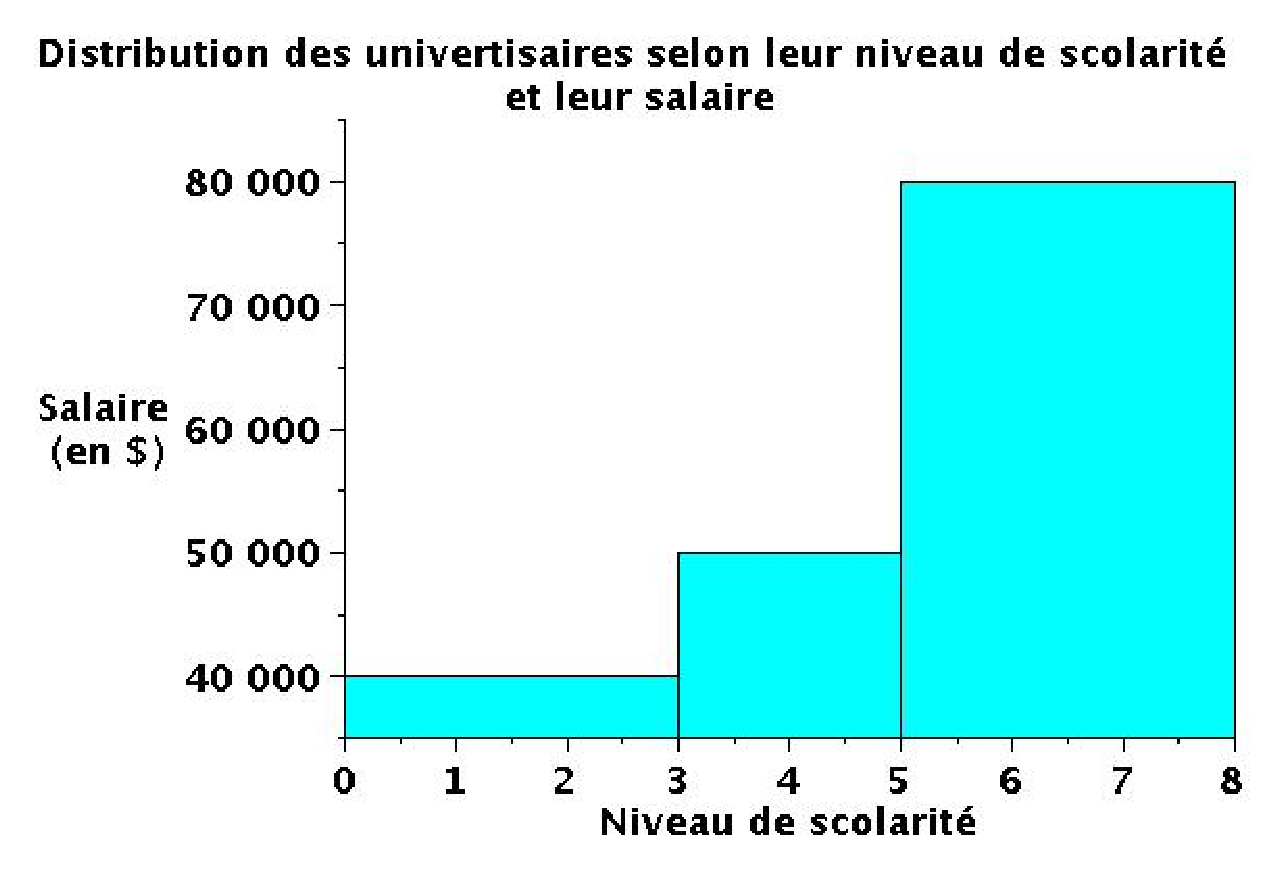
\includegraphics[width=8cm,bb=14 14 611 415]{Q2008v.eps}
 % Q2008v.eps: 1179666x1179666 pixel, 300dpi, 9987.84x9987.84 cm, bb=14 14 611 415
\end{center}

What type of graph is it?\\
a$)$ Bar chart\\
b$)$ Stem and leaf diagram\\
c$)$ Pie chart\\
d$)$ Histogram\\

R\'eponse : d$)$\\

R\'etroaction :
\begin{center}
 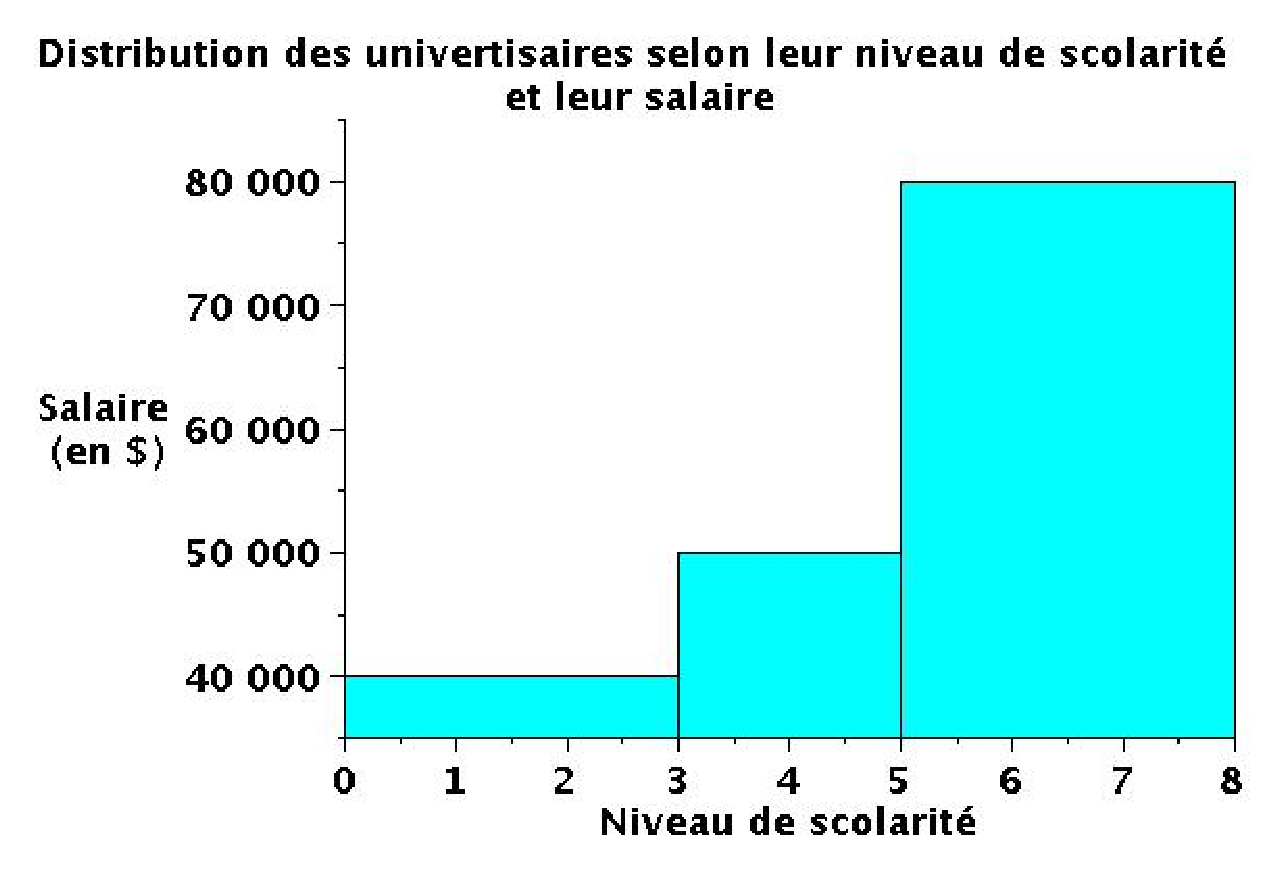
\includegraphics[width=8cm,bb=14 14 611 415]{Q2008v.eps}
 % Q2008v.eps: 1179666x1179666 pixel, 300dpi, 9987.84x9987.84 cm, bb=14 14 611 415
\end{center}
We want to know what type of graph this is.\\
\begin{itemize}
 \item Bar charts bars are all the same width.\\
 \item Stem and leaf diagrams bars are made of numbers.\\
 \item Pie charts are shaped like a circle.\\
 \item Histograms are made of bars that can have different widths and different heights.\\
\end{itemize}
Consequently, the answer is d).\\

2009-- In statistics, what is the most frequent data called?\\

a$)$ Frequency \\
b$)$ Median\\
c$)$ Fashion\\
d$)$ Mode\\

R\'eponse : d$)$\\

R\'etroaction :\\
In a date set, the most frequent data is called the mode.\\
Consequently, the answer is d).\\

%Questions statistiques mathematiques 416 difficulte 2
%Etudes statistiques

2010-- What is a statistical study that studies different characteristics of each member of a population called? \\

a$)$ A poll\\
b$)$ A census\\
c$)$ A survey\\
d$)$ A phone survey\\

R\'eponse : b$)$\\

R\'etroaction :\\
A census is a statistical study that looks at different characteristics of each member of a population. For example, if a small business owner wants to know how many years of experience and what kind of backgrounds his employees have, he must run a census. \\
Consequently, the answer is b).\\

2011-- Andreas wants to collect data to find out if the students are witnessing violence at his school. He says he can use a written questionnaire to collect his data. Is this true or false?\\

R\'eponse : Vrai\\

R\'etroaction :\\
A written questionnaire is a method that may be used to collect data. \\
Consequently, the answer is : true.\\

%Echantillonnage (Sampling)

2012-- What sampling method can be used if the population is divided into groups? \\

a$)$ Simple random sampling.\\
b$)$ Stratified sampling.\\
c$)$ Cluster sampling.\\
d$)$ Group sampling.\\


R\'eponse : c$)$\\

R\'etroaction :\\
Cluster sampling is a sampling method where the entire population is divided into groups, or clusters, and a random sample of these clusters are selected. All observations in the selected clusters are included in the sample.\\
Consequently, the answer is c).\\

2013-- One can use a sample that is non-representative of the population to extrapolate a poll's results. True or false? \\

R\'eponse : Faux\\

R\'etroaction :\\
A sample must be representative of the population to ensure the validity of a poll's results.\\
Consequently, the answer is : false.\\

%Quartiles

2014-- Here are the top 10 results of a French competition. What is the median of this data set?  \\
\begin{center}
 \begin{tabular}{|c  c  c  c  c|} \hline

95 & 95 & 96 & 96 & 96 \\
98 & 98 & 99 & 99 & 100 \\ \hline

\end{tabular}
\end{center}

R\'eponse : 97\\

R\'etroaction :\\
\begin{center}
 \begin{tabular}{|c  c  c  c  c|} \hline

95 & 95 & 96 & 96 & 96 \\
98 & 98 & 99 & 99 & 100 \\ \hline

\end{tabular}
\end{center}
Since the data set size is even, the median is the arithmetic mean of the 2 data points in the middle of the ordered data set. Since there are 10 values in the set, one must take the average of the fifth and the sixth value.\\
\begin{equation*}
 \frac{96+98}{2}=97
\end{equation*}
Consequently, the answer is 97.\\

2015-- Here are Catherine's best 10 high school marks. What is the value of the first quartile?
\begin{center}
 \includegraphics[width=6cm,height=8cm,angle=-90]{Q2015.eps}
 % Graph.eps: 1048576x0 pixel, 0dpi, infxnan cm, bb=
\end{center}


a$)$ 95\\
b$)$ 96\\
c$)$ 99\\
d$)$ 100\\

R\'eponse : b$)$\\

R\'etroaction :
\begin{center}
 \includegraphics[width=6cm,height=8cm,angle=-90]{Q2015.eps}
 % Graph.eps: 1048576x0 pixel, 0dpi, infxnan cm, bb=
\end{center}
We are looking for the first quartile value.\\
In the graph, quartiles are found by locating "whiskers". A whisker is a vertical mark in the box plot. The first whisker is located at 96.\\
Consequently, the answer is b).\\

%Mesures de position

2016-- The rank fifth is a position measurement. The first rank fifth is associated with :\\

a$)$ the five lower results.\\
b$)$ the best results.\\
c$)$ the worse results.\\
d$)$ the first values of the set.\\

R\'eponse : b$)$\\

R\'etroaction :\\
When the rank fifth is used as a position measurement, the first rank fifth is associated to the best results.\\
Consequently, the answer is b).\\

2017-- The percentile is a position measurement. A value whose percentile is one is associated to: \\

a$)$ a central position in the data set.\\
b$)$ a median position in the data set.\\
c$)$ the best results.\\
d$)$ the worse results.\\

R\'eponse : d$)$\\

R\'etroaction :\\
When the percentile is used a position measurement, a percentile of one is associated to the worse results. The percentile indicated the percentage of data that is less than or equal to the considered value. \\
Consequently, the answer is d).\\

%Interpretation des donnees

2018-- Telworld is a phone company that offers services to its clients. Its president would like to offer more services. Since he wants to offer services that would be profitable to his company, he hires a survey firm to ask his clients about the particular needs they might have. What is the character of this survey? \\

a$)$ The number of phones per household.\\
b$)$ The particular needs of clients.\\
c$)$ The company's clients.\\
d$)$ The services used by clients.\\

R\'eponse : b$)$\\

R\'etroaction :\\
The character is what the statistical study is about. The purpose of this survey is to find out about the particular needs of the company's clients.\\
Consequently, the answer is b).\\

2019--  Marc fait du b\'en\'evolat pour acqu\'erir de l'exp\'erience en soin des personnes \`a mobilit\'e r\'eduite.  Il peut travailler jusqu'\`a 10 heures certaines semaines, alors que, d'autres semaines, il ne travaille pas du tout. Voici la distribution du nombre d'heures qu'il a fait dans les trois derniers mois selon la fr\'equence.\\
\begin{center}
 \begin{tabular}{|c|c|} \hline
{\bf Nombre d'heures} & {\bf Fr\'equence}  \\ \hline \hline

[0-2] & 3 \\ \hline
]2-4] & 0 \\ \hline
]4-6] & 1 \\ \hline
]6-8] & 5 \\ \hline
]8-10] & 3 \\ \hline
\multicolumn{2}{c}{}\\
\end{tabular}\\
\end{center}


Quelle est la classe modale de la distribution?\\

a$)$ [0-2]\\ [2mm]
b$)$ ]2-4]\\[2mm]
c$)$ ]4-6]\\[2mm]
d$)$ ]6-8]\\

R\'eponse : d$)$\\

R\'etroaction :\\
\begin{center}
 \begin{tabular}{|c|c|} \hline
{\bf Nombre d'heures} & {\bf Fr\'equence}  \\ \hline \hline

[0-2] & 3 \\ \hline
]2-4] & 0 \\ \hline
]4-6] & 1 \\ \hline
\textbf{]6-8]} & \textbf{5} \\ \hline
]8-10] & 3 \\ \hline
\multicolumn{2}{c}{}\\
\end{tabular}\\
\end{center}
La classe modale d'une distribution \`a donn\'ees regroup\'ees en classes est la classe dans laquelle il y a le plus grand effectif.\\
Par cons\'equent, la r\'eponse est d).\\

%Questions statistiques mathematiques 416 difficulte 3
%Etudes statistiques

2020-- Un diagramme de quartiles permet de tirer certaines conclusions sur un ensemble de donn\'ees. Quelles sont ces conclusions? \\

\begin{quote}
1. La concentration des donn\'ees \\
2. La dispersion des donn\'ees\\
3. La moyenne des donn\'ees\\
4. L'effectif des donn\'ees\\
\end{quote}

a$)$ 1 et 2\\
b$)$ 1 et 3\\
c$)$ 1 et 4\\
d$)$ 2 et 4\\

R\'eponse : a$)$\\

R\'etroaction :\\
Un diagramme de quartiles permet de tirer certaines conclusions sur l'\'etendue et sur la dispersion des donn\'ees. On ne peut cependant pas tirer de conclusions quant \`a la moyenne et l'effectif des donn\'ees.\\
Par cons\'equent, la r\'eponse est a).\\

2021-- Dans une \'etude statistique, un \'echantillon est repr\'esentatif de la population lorsque l'\'echantillon a une caract\'eristique identique \`a la population. Est-ce vrai ou faux?\\

R\'eponse : Faux\\

R\'etroaction :\\
Un \'echantillon est repr\'esentatif de la population s'il poss\`ede toutes les caract\'eristiques de la population. \\
Par cons\'equent, la r\'eponse est: faux.\\

%Echantillonnage

2022-- Carl veut savoir quel type de f\^ete les \'el\`eves de son \'ecole veulent pour la fin de l'ann\'ee scolaire. Pour choisir les personnes qu'il interrogera, il prend le bottin t\'el\'ephonique de son \'ecole et il appelle le septi\`eme \'el\`eve de chaque page pour lui poser des questions. Quel type d'\'echantillonnage a-t-il utilis\'e ?\\

a$)$ \'Echantillonnage al\'eatoire\\
b$)$ \'Echantillonnage par grappes\\
c$)$ \'Echantillonnage stratifi\'e\\
d$)$ \'Echantillonnage syst\'ematique\\

R\'eponse : d$)$\\

R\'etroaction :\\
\begin{itemize}
 \item L'\'echantillonnage al\'eatoire consiste \`a choisir au hasard l'ensemble des individus de l'\'echantillon. \\
\item L'\'echantillonnage par grappes est utilis\'e lorsque la population est divis\'ee en groupes. Cela consiste \`a prendre comme \'echantillon l'ensemble des individus composant les grappes qui ont \'et\'e choisies au hasard. \\
\item L'\'echantillonnage stratifi\'e consiste \`a diviser la population en strates. Chaque strate dans l'\'echantillon est repr\'esent\'ee dans le m\^eme rapport que dans la population. Enfin, les individus de chaque strate sont s\'electionn\'es au hasard pour faire partie de l'\'echantillon. \\
\item L'\'echantillonnage syst\'ematique consiste \`a choisir au hasard un premier individu puis \`a s\'electionner les autres selon un m\^eme proc\'ed\'e. \\
\end{itemize}
Par cons\'equent, la r\'eponse est d).\\

2023-- Lucie veut savoir si une question qu'elle veut mettre dans un sondage contient une source de biais. Voici sa question: \og Ne croyez-vous pas que l'\'ecole devrait commencer \`a midi?  \fg.\\
Qu'en penses-tu? \\

a$)$ Sa question contient une source de biais.\\
b$)$ Sa question ne contient pas de source de biais.\\
c$)$ Tu penses que l'\'ecole devrait commencer \`a midi.\\
d$)$ Une question ne peut pas contenir une source de biais.\\

R\'eponse : a$)$\\

R\'etroaction :
\begin{center}
 \og Ne croyez-vous pas que l'\'ecole devrait commencer \`a midi?  \fg.
\end{center}
La formulation d'une question peut-\^etre une source de biais. Dans la question de Lucie, il est sugg\'er\'e au r\'epondant qu'il croit que l'\'ecole devrait commencer \`a midi. Il y a donc une source de biais. \\
Par cons\'equent, la r\'eponse est a).\\

%Quartiles

2024-- Pierre-Luc, Carl, Didier et Francis tentent d'interpr\'eter le diagramme de quartiles suivant:
\begin{center}
 \includegraphics[width=6cm,height=8cm,angle=-90]{Q2024.eps}
 % Q2024.eps: 1048576x0 pixel, 0dpi, infxnan cm, bb=
\end{center}

Qui des quatre gar\c cons donne une affirmation qui est clairement fausse?\\

a$)$ Carl dit que l'\'etendue interquartile vaut 3. \\
b$)$ Didier dit que les donn\'ees sont plus concentr\'ees dans le deuxi\`eme quartile.\\
c$)$ Francis dit que la m\'ediane est 4.\\
d$)$ Pierre-Luc dit qu'il y a plus de donn\'ees dans le quatri\`eme quartile. \\

R\'eponse : d$)$\\

R\'etroaction :\\
Pierre-Luc fait une erreur en disant que le quatri\`eme quartile contient le plus de donn\'ees puisque chaque quart contient le m\^eme nombre de donn\'ees. \\
Par cons\'equent, la r\'eponse est d).\\

2025-- Maxime a un diagramme de quartile, mais il n'a pas les donn\'ees qui ont servi \`a le construire. Comment peut-il calculer la moyenne des donn\'ees?\\

a$)$ Il doit faire la moyenne arithm\'etique du minimum et du maximum des donn\'ees. \\
b$)$ Il doit faire la moyenne arithm\'etique du minimum, des quartiles et du maximum des donn\'ees. \\
c$)$ Il n'a qu'\`a prendre la m\'ediane des donn\'ees, c'est la m\^eme chose que la moyenne.\\
d$)$ Il ne peut pas calculer la moyenne \`a partir du diagramme, il lui aurait fallu avoir les donn\'ees initiales.\\
\begin{center}
 \includegraphics[width=6cm,height=8cm,angle=-90]{Q2024.eps}
 % Q2024.eps: 1048576x0 pixel, 0dpi, infxnan cm, bb=
\end{center}

R\'eponse : d$)$\\

R\'etroaction :\\
Le diagramme de quartiles permet de tirer certaines conclusions g\'en\'erales sur les donn\'ees, mais on ne peut pas en d\'eduire la moyenne. Il faut disposer des donn\'ees initiales pour la calculer.\\
Par cons\'equent, la r\'eponse est d).\\

%Mesures de position

2026-- Mariannik travaille dans une boutique de v\^etements pour femmes. \`A la fin de sa journ\'ee, elle regarde les montants des ventes de la journ\'ee. Elle les entre dans un logiciel et fait imprimer un diagramme circulaire \`a partir des donn\'ees.
\begin{center}
 \includegraphics[width=8cm]{Q2058b.eps}
 % Q2058b.eps: 1179666x1179666 pixel, 0dpi, infxinf cm, bb=
\end{center}
Sa coll\`egue Maude lui dit que son graphique ne sert \`a rien.\\
Pourquoi dit-elle \c ca?\\

a$)$ Le diagramme circulaire a trop de couleurs.\\
b$)$ Le diagramme circulaire montre l'importance relative d'une vente par rapport aux autres, il ne permet pas de voir l'ensemble de la situation des ventes.\\
c$)$ Le diagramme circulaire ne permet pas de voir l'importance relative d'une vente par rapport aux autres.\\
d$)$ Le diagramme circulaire n'est pas adapt\'e pour les montants de vente.\\

R\'eponse : b$)$\\

R\'etroaction :\\
Maude dit que le graphique ne sert \`a rien, car il montre l'importance relative d'une facture par rapport aux autres. Il ne permet pas de voir l'ensemble de la situation des ventes alors que c'est cela qu'il serait pertinent d'\'etudier dans cette situation.\\
Par cons\'equent, la r\'eponse est b).\\

2027-- Le proc\'ed\'e de cueillette de donn\'ees et le type d'\'etude statistique sont une seule et m\^eme chose. Est-ce vrai ou faux?\\

R\'eponse : Faux\\

R\'etroaction :\\
Le proc\'ed\'e de cueillette de donn\'ees est le moyen pris pour recueillir les informations. Le type d'\'etude statistique est la m\'ethode utilis\'ee pour \'etudier une population.\\
Par cons\'equent, la r\'eponse est: faux.\\

%Interpretation des donnees

2028-- Un sondage a \'et\'e r\'ealis\'e aupr\`es de 1000 hommes et femmes de la province de Qu\'ebec pour conna\^itre leurs habitudes t\'el\'evisuelles. \`A la question sur le nombre d'heures qu'ils passent devant la t\'el\'evision, voici le diagramme de quartile repr\'esentant ce que les sond\'es ont r\'epondu:
\begin{center}
 \includegraphics[width=6cm,height=8cm,angle=-90]{Q2028.eps}
 % Q2028.eps: 1048592x1048592 pixel, 0dpi, infxinf cm, bb=
\end{center}

Quelle affirmation est fausse?\\

a$)$ En moyenne, les sond\'es \'ecoutent la t\'el\'evision 15 heures par semaine.\\
b$)$ Il y a autant de sond\'es qui \'ecoutent la t\'el\'evision entre 0 et 10 heures par semaine qu'entre 10 et 15 heures.\\
c$)$ Il y a des sond\'es qui n'\'ecoutent pas la t\'el\'evision.\\
d$)$ La moiti\'ee des sond\'es \'ecoute la t\'el\'evision entre 10 et 20 heures par semaine.\\

R\'eponse : a$)$\\

R\'etroaction :\\
Dans un diagramme de quartiles, il n'est pas possible de calculer la moyenne des donn\'ees.\\
Par cons\'equent, la r\'eponse est a).\\

2029-- Un sondage a \'et\'e r\'ealis\'e aupr\`es de 1000 hommes et femmes de Livreville pour conna\^itre leurs habitudes de lecture. \`A la question sur le nombre de livres qu'ils lisent par ann\'ee, voici ce que les sond\'es ont r\'epondu.
\begin{center}
 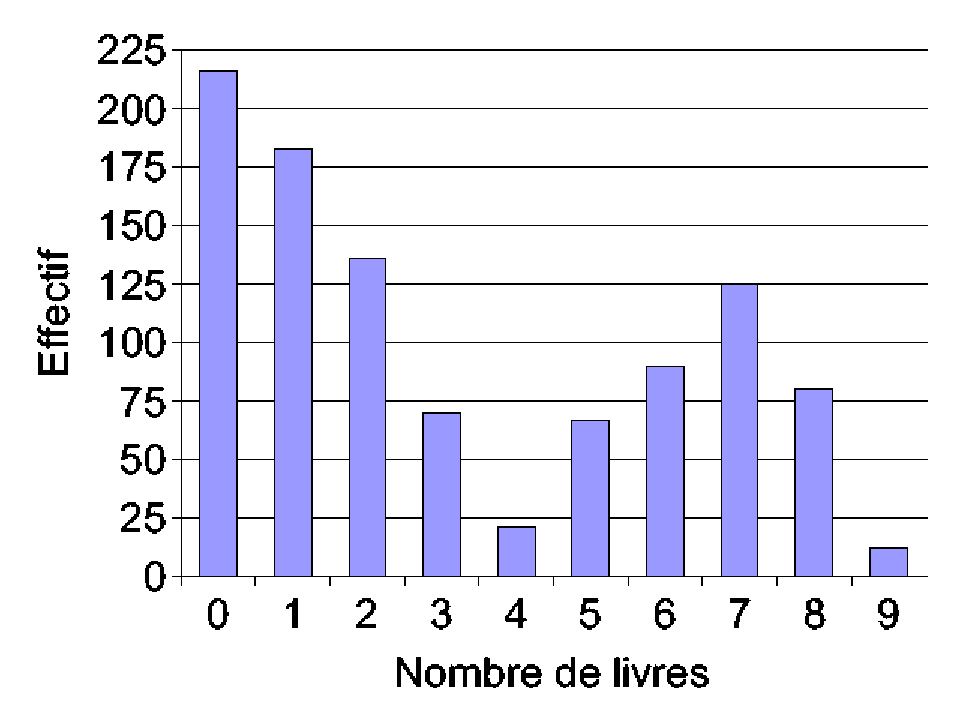
\includegraphics[width=6cm]{GraphLivreEPS.eps}
 % GraphLivreEPS.eps: 1048592x1048592 pixel, 0dpi, infxinf cm, bb=
\end{center}

Parmi les conclusions suivantes, laquelle est fausse?\\

a$)$ Le mode de cette distribution est z\'ero livre.\\
b$)$ Le mode de cette distribution se trouve entre 200 et 225 personnes.\\
c$)$ Plus de la moiti\'e des sond\'es lisent deux livres ou moins par ann\'ee.\\
d$)$ Une grande proportion des sond\'es ne lisent aucun livre dans une ann\'ee.\\

R\'eponse : b$)$\\

R\'etroaction :
\begin{center}
 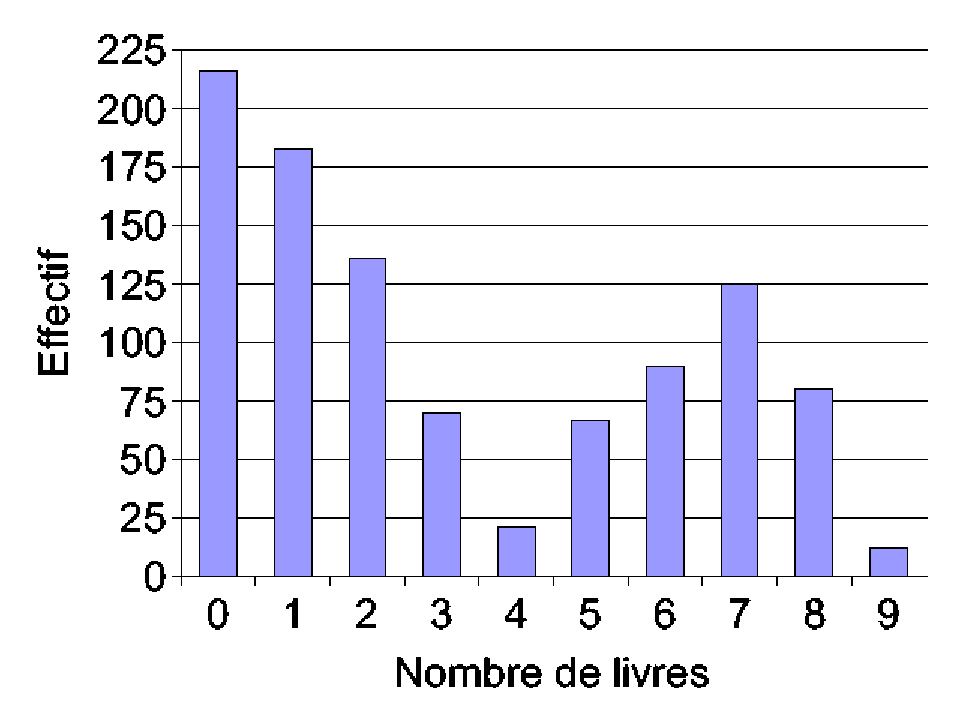
\includegraphics[width=6cm]{GraphLivreEPS.eps}
 % GraphLivreEPS.eps: 1048592x1048592 pixel, 0dpi, infxinf cm, bb=
\end{center}
On cherche la conclusion qui est fausse.\\
\begin{itemize}
 \item Le mode de cette distribution est z\'ero livre.
 \item Le mode de cette distribution se trouve entre 200 et 225 personnes.
 \item Plus de la moiti\'e des sond\'es lisent deux livres ou moins par ann\'ee.
 \item Une grande proportion des sond\'es ne lisent aucun livre dans une ann\'ee.\\
\end{itemize}
Dans une distribution de donn\'ees, la donn\'ee la plus fr\'equente est le mode. Dans cette distribution, on a que le mode est z\'ero et que l'\textbf{effectif} du mode est entre 200 et 225 personnes.\\
Par cons\'equent, la r\'eponse est b).\\

%Questions statistiques mathematiques 416 difficulte 4
%Etudes statistiques

2030-- Comment nomme-t-on le sujet sur lequel porte une \'etude statistique?\\

a$)$ La suggestion\\
b$)$ La taille\\
c$)$ Le caract\`ere\\
d$)$ Le sujet\\

R\'eponse : c$)$\\

R\'etroaction :\\
Le caract\`ere est ce sur quoi porte une \'etude statistique.\\
Par cons\'equent, la r\'eponse est c$)$.\\

2031-- Luc veut savoir si les \'el\`eves de sa classe prendront une option en sciences l'ann\'ee prochaine. Il souhaite avoir une r\'eponse pr\'ecise et il est pr\^et \`a effectuer soit un sondage soit un recensement. Alexandra lui dit de faire un recensement puisque cette m\'ethode a un degr\'e d'incertitude moins \'elev\'e qu'un sondage. Est-ce vrai ou faux? \\

R\'eponse : Vrai\\

R\'etroaction :\\
Un recensement permet de conna\^itre pr\'ecis\'ement un caract\`ere d'une population puisqu'il v\'erifie ce caract\`ere aupr\`es de chacun des \'el\'ements de la population. \\
Par cons\'equent, la r\'eponse est: vrai.\\

%Echantillonnage

2032-- Caroline, Christine, M\'elissa et Marie doivent faire un \'echantillon stratifi\'e. Caroline dit que chaque strate doit contenir le m\^eme nombre d'individus. Christine dit que la premi\`ere strate doit contenir un individu, la deuxi\`eme 2 individus, la troisi\`eme 3 individus, etc. M\'elissa dit que chaque strate doit contenir un nombre d'individus dans le m\^eme rapport dans l'\'echantillon que dans la population. Marie, quant \`a elle, dit qu'un seul individu par strate est suffisant pour bien repr\'esenter la population. Qui a raison? \\

a$)$ Caroline\\
b$)$ Christine\\
c$)$ Marie\\
d$)$ M\'elissa\\

R\'eponse : d$)$\\

R\'etroaction :\\
Dans un \'echantillon stratifi\'e, chaque strate doit contenir un nombre d'individus dans un m\^eme rapport dans l'\'echantillon que dans la population.\\
Par cons\'equent, la r\'eponse est d).\\

2033-- Le centre sportif \og En Sant\'e \fg \,a 1000 membres. Le g\'erant de l'\'etablissement veut conna\^itre les habitudes alimentaires de ses membres afin de savoir s'il devrait offrir un service de nutrition. Pour former son \'echantillon, il h\'esite entre plusieurs options. Aide-le \`a choisir la meilleure option.\\

a$)$ Choisir al\'eatoirement 20 individus dans la salle de sport \`a tous les lundis midis pendant 4 semaines.\\
b$)$ Diviser la client\`ele en strates selon l'\^age et le sexe des personnes et faire un \'echantillon stratifi\'e de 50 individus.\\
c$)$ Laisser un ordinateur choisir al\'eatoirement un \'echantillon de 100 individus parmi la banque des membres.\\
d$)$ Prendre la liste des membres et choisir tout ceux qui sont inscrit au centre depuis plus de 4 ans. \\

R\'eponse : c$)$\\

R\'etroaction :\\
Si on choisit al\'eatoirement 20 individus dans la salle de sport \`a tous les lundis midis durant 4 semaines, l'\'echantillon est biais\'ee puisque ce sont habituellement les m\^emes personnes qui viennent \`a la m\^eme heure pour une journ\'ee fixe. Prendre les membres qui sont inscrits au centre depuis plus de 4 ans ne permet pas d'avoir un \'echantillon qui repr\'esente bien l'ensemble des membres. Diviser la client\`ele en strates selon l'\^age et le sexe des personnes et faire un \'echantillon stratifi\'e de 50 individus ou laisser un ordinateur choisir al\'eatoirement un \'echantillon de 100 individus parmi la banque des membres sont de bonnes fa\c cons de faire l'\'echantillon. Comme la deuxi\`eme option donne plus d'individus pour l'\'echantillon, alors c'est la meilleure option.\\
Par cons\'equent, la r\'eponse est c).\\

%Quartiles

2034-- Dans un diagramme de quartiles, combien retrouve-t-on de quartiles?\\

a$)$ 2\\
b$)$ 3\\
c$)$ 4\\
d$)$ 5\\

R\'eponse : b$)$\\

R\'etroaction :\\
Dans un diagramme de quartiles, on retrouve quatre quarts s\'epar\'es par trois quartiles. \\
Par cons\'equent, la r\'eponse est b).\\\\

2035-- Dans quel quart les donn\'ees de ce diagramme de quartiles sont-elles les plus dispers\'ees?
\begin{center}
 \includegraphics[width=6cm,height=8cm,angle=-90]{Q2035.eps}
 % Q2035.eps: 1048592x1048592 pixel, 0dpi, infxinf cm, bb=
\end{center}

a$)$ Premier quart\\
b$)$ Deuxi\`eme quart\\
c$)$ Troisi\`eme quart\\
d$)$ Quatri\`eme quart\\

R\'eponse : d$)$\\

R\'etroaction :\\
Dans le diagramme, on peut remarquer que le quatri\`eme quart est beaucoup plus long que les autres. On peut donc conclure que c'est dans ce quart que les donn\'ees sont les plus dispers\'ees. \\
Par cons\'equent, la r\'eponse est d).\\

%Mesures de position

2036-- Marc doit attribuer des rangs cinqui\`emes \`a cette s\'erie de donn\'ees:
\begin{quote}
4, 4, 5, 5, 5, 5, 5, 6, 6, 6, 7, 7, 8, 8, 8, 8, 8, 8, 9, 9, 9, 9, 10, 10, 10, 11, 11
\end{quote}
Voici le r\'esultat auquel il est arriv\'e:\\
\begin{tabular}{| c | c | c | c | c|} \hline
{\bf Cinqui\`eme rang } & {\bf Quatri\`eme rang} & {\bf Troisi\`eme rang } & {\bf Deuxi\`eme rang} & {\bf Premier rang}\\ \hline \hline

4 & 6 & 8 & 8 & 10\\
4 & 6 & 8 & 9 & 10 \\
5 & 6 & 8 & 9 & 10 \\
5 & 7 & 8 & 9 & 11 \\
5 & 7 & 8 & 9 & 11 \\
5 &  &  &  &  \\
5 &  &  &  &  \\
\hline

\end{tabular}\\ \\
A-t-il bien attribu\'e les rangs? Oui ou non?\\

R\'eponse : Non\\

R\'etroaction :\\
\begin{tabular}{| c | c | c | c | c|} \hline
{\bf Cinqui\`eme rang } & {\bf Quatri\`eme rang} & {\bf Troisi\`eme rang } & {\bf Deuxi\`eme rang} & {\bf Premier rang}\\ \hline \hline

4 & 6 & 8 & 8 & 10\\
4 & 6 & 8 & 9 & 10 \\
5 & 6 & 8 & 9 & 10 \\
5 & 7 & 8 & 9 & 11 \\
5 & 7 & 8 & 9 & 11 \\
5 &  &  &  &  \\
5 &  &  &  &  \\
\hline

\end{tabular}\\ \\
Le deuxi\`eme et le troisi\`eme rang cinqui\`eme contiennent tous les deux la donn\'ee 8, mais les donn\'ees \'egales doivent avoir le m\^eme rang. \\
Par cons\'equent, la r\'eponse est: non.\\

2037-- Voici les r\'esultats d'une comp\'etition de patinage de vitesse courte piste du circuit du Qu\'ebec:
\begin{quote}
6, 9, 11, 14, 16, 17, 21, 29, 35, 35, 37, 37, 37, 40, 45, 53, 60, 65, 69, 71, 80, 93, 98, 104, 130, 176, 200
\end{quote}
Le m\'edaill\'e d'or a eu un r\'esultat de 200. Quel est le rang centile de Charles s'il a eu une note de 104? \\

a$)$ 13\\
b$)$ 15\\
c$)$ 85\\
d$)$ 89\\

R\'eponse : d$)$\\

R\'etroaction :\\
Il y a 24 des 27 participants qui ont eu un r\'esultat inf\'erieur ou \'egal au r\'esultat de Charles. Il faut donc calculer en pourcentage ce que vaut $\frac{24}{27}$ . \\
On calcule donc:  \\
\begin{equation*}
\frac{24}{27}\times 100 \approx \frac{88,8}{100}
\end{equation*}
Comme la r\'eponse n'est pas un entier, il faut arrondir \`a l'entier sup\'erieur.\\
Par cons\'equent, la r\'eponse est d$)$.\\

%Interpretation des donnees

2038-- Voici des donn\'ees que Chantal a r\'ecup\'er\'ees sur Internet concernant le nombre de jours d'hibernation des ours que l'on retrouve aux parc nationaux de Banff et de Jasper.
\begin{center}
 \begin{tabular}{| c | c |} \hline
{\bf Nombre de jours } & {\bf Fr\'equence} \\ \hline \hline

]150-160] & 12 \\
]160-170] & 26 \\
]170-180] & 35  \\
]180-190] & 38  \\
]190-200] & 19  \\
]200-210] & 7   \\

\hline
\end{tabular}
\end{center}
Elle d\'ecide de faire un diagramme pour mieux voir et interpr\'eter les donn\'ees.
\begin{center}

 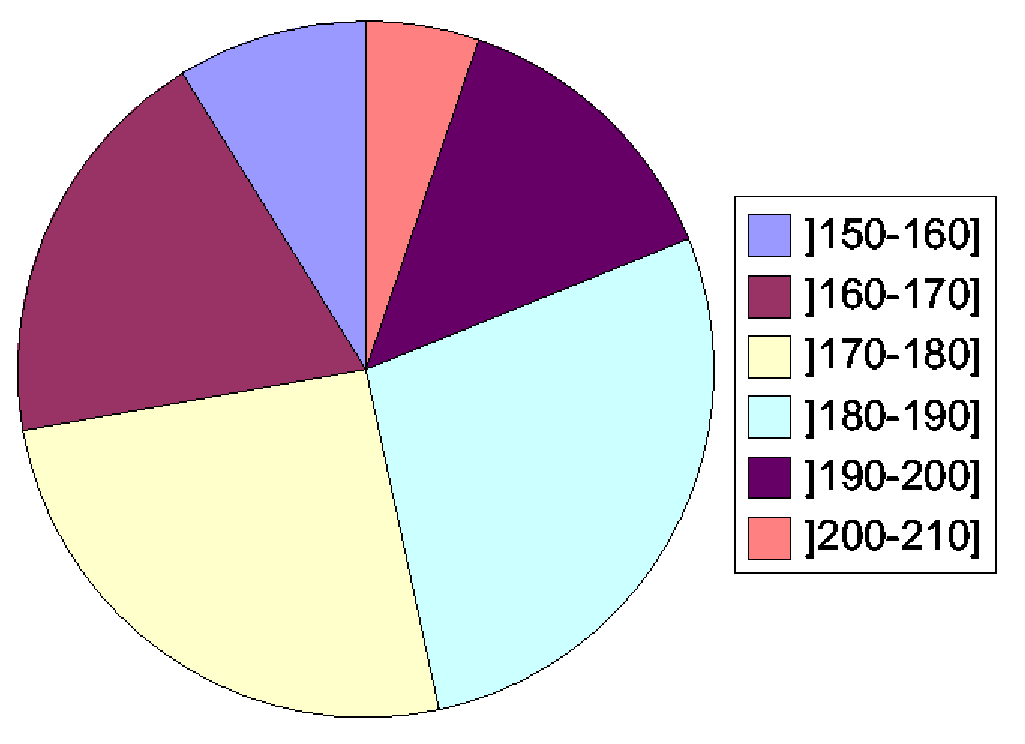
\includegraphics[width=6cm]{graphQ2038.eps}
 % graphQ2038.eps: 1048592x1048592 pixel, 0dpi, infxinf cm, bb=

\end{center}
Chantal dit qu'elle a fait un bon choix de graphique puisque son but \'etait de montrer l'importance relative du nombre d'ours selon le nombre de jours d'hibernation. Est-ce qu'elle dit vrai ou faux?\\

R\'eponse : Vrai\\

R\'etroaction :\\
Un diagramme circulaire est id\'eal pour montrer l'importance relative du nombre d'ours selon le nombre de jours d'hibernation. \\
Par cons\'equent, la r\'eponse est: vrai.\\

2039-- Voici le diagramme \`a feuilles et \`a tiges des montants de 50 dons recueillis par une fondation lors d'une activit\'e de lev\'ee de fonds.\\
\begin{center}
 \begin{tabular}{|c|l|}
\multicolumn{2}{c}{\bf Montants des dons recueillis} \\  \hline

0 & 2-5-5-5 \\ \hline
1 & 0-0-0-0-0-5-5-5 \\ \hline
2 & 0-0-0-0-0-0-0-0-0-0-0-0-0-5-5-5 \\ \hline
3 & 0-0-0-0-0-0-0-5-5 \\ \hline
4 & 0-0-0-0-0-0-0-0-0-5-5-5-5 \\ \hline
\multicolumn{2}{c}{}\\
\end{tabular}
\end{center}
On d\'ecide de faire un diagramme de quartiles \`a partir de cette distribution. Lequel de ces \'enonc\'es est faux?\\

a$)$ La m\'ediane est 22,5.\\
b$)$ Les donn\'ees du deuxi\`eme quartile sont les plus concentr\'ees.\\
c$)$ Les donn\'ees les plus dispers\'ees sont dans le premier quartile.\\
d$)$ L'\'etendue interquartile est de 5. \\

R\'eponse : d$)$\\

R\'etroaction :\\
\begin{center}
 \begin{tabular}{|c|l|}
\multicolumn{2}{c}{\bf Montants des dons recueillis} \\  \hline

0 & 2-5-5-5 \\ \hline
1 & 0-0-0-0-0-5-5-5 \\ \hline
2 & 0-0-0-0-0-0-0-0-0-0-0-0-0-5-5-5 \\ \hline
3 & 0-0-0-0-0-0-0-5-5 \\ \hline
4 & 0-0-0-0-0-0-0-0-0-5-5-5-5 \\ \hline
\multicolumn{2}{c}{}\\
\end{tabular}
\end{center}
Pour calculer l'\'etendue interquartile, il faut faire la diff\'erence entre les valeurs du premier et du troisi\`eme quartile. Comme on  a 50 valeurs ordonn\'ees, la valeur du premier quartile sera celle de la 13\ieme{} donn\'ee et la valeur du troisi\`eme quartile sera celle de la 38\ieme{} donn\'ee. \\
On calcule donc:\\
\begin{equation*}
 \textrm{Q$_{3}$ - Q$_{1}$}=40-20 = 20 \neq 5
\end{equation*}
Par cons\'equent, la r\'eponse est d).\\

%Questions statistiques mathematiques 416 difficulte 5
%Etudes statistiques

2040-- Luc lit le journal et il trouve un article qu'il lit \`a Mireille. Voici ce que lit Luc:
\begin{center}
 \og Les ovnis existent. Selon un sondage, plus de la moiti\'e des habitants de Smallville ont vu des ovnis voler dans le ciel. \fg
\end{center}
Mireille lui dit que ce n'est pas s\'erieux et qu'on ne peut pas croire ce qui est \'ecrit dans le journal puisque de toute fa\c con, ce n'est qu'un sondage et non pas une enqu\^ete ou un recensement. Luc dit, quant \`a lui, que lorsqu'un sondage est bien effectu\'e, il peut \^etre aussi fiable qu'une enqu\^ete ou un recensement. Qui dit vrai?\\

R\'eponse : Luc\\

R\'etroaction :\\
Lorsqu'un sondage est bien effectu\'e, on peut croire que l'image de la situation est assez pr\'ecise pour s'y fier. \\
Par cons\'equent, la r\'eponse est: Luc.\\

2041-- Voici les notes du dernier test d'\'education physique de la
classe de Sophie.
\begin{quote}
 70, 70, 72, 75, 75, 80, 83, 74, 86, 87, 87, 89, 92, 92, 92
\end{quote}
Quel est le rang centile de Sophie si elle a eu une note de 80? \\

R\'eponse : 40\\

R\'etroaction :\\
Il y a 6 des 15 \'el\`eves de la classe qui ont eu une note inf\'erieure ou \'egale \`a la note de Sophie. Il s'agit donc de calculer en pourcentage ce que vaut $\frac{6}{15}$ . On calcule donc:  \\
\begin{equation*}
 \frac{6}{15} \times 100 = 40
\end{equation*}
Par cons\'equent, la r\'eponse est 40.\\

%Echantillonnage

2042-- Le menu de la caf\'et\'eria de l'\'ecole secondaire Sainte-Foy-de-Vau fait peur aux \'el\`eves de l'\'ecole. Didier en a assez et d\'ecide de sugg\'erer un nouveau menu \`a la direction de l'\'ecole. Il d\'ecide d'interroger des \'el\`eves pour pouvoir cr\'eer une proposition de nouveau menu. Il pr\'epare ses questions et s'installe \`a la sortie de la caf\'et\'eria \`a la fin du d\^iner pour les poser aux quelques \'el\`eves qui la fr\'equentent.  M\^eme s'il est press\'e de retourner en cours et qu'il demande aux \'el\`eves de r\'epondre rapidement, il r\'eussit \`a obtenir quelques r\'eponses. Avec les r\'eponses obtenues, il \'ecrit une suggestion qu'il pr\'esente \`a la direction de l'\'ecole. Quelles sont les sources de biais retrouv\'ees dans ce sondage? \\
\begin{quote}
1. La cueillette de donn\'ees\\
2. L'attitude du sondeur\\
3. La formulation des questions\\
4. L'\'echantillonnage\\
\end{quote}


a$)$ 1 et 2 \\
b$)$ 1, 2 et 4 \\
c$)$ 2, 3 et 4 \\
d$)$ 2 et 4 \\


R\'eponse : d$)$\\

R\'etroaction :\\
Didier n'a pas adopt\'e une bonne attitude en demandant aux \'el\`eves de lui r\'epondre rapidement. De plus, il a seulement pos\'e ses questions \`a des \'el\`eves qui fr\'equentent la caf\'et\'eria, ce qui ne fait pas un bon \'echantillonnage. \\
Par cons\'equent, la r\'eponse est d).\\

2043-- La pr\'ecision et la fiabilit\'e des r\'esultats d'un sondage d\'ependent de certains facteurs. Quels sont-ils? \\

a$)$ La repr\'esentativit\'e et la taille de l'\'echantillon. \\
b$)$ La taille de l'\'echantillon et le type de cueillette de donn\'ees. \\
c$)$ Le s\'erieux des sondeurs et des individus de l'\'echantillon. \\
d$)$ Le type de cueillette de donn\'ees et le caract\`ere \'etudi\'e. \\

R\'eponse : a$)$\\

R\'etroaction :\\
La repr\'esentativit\'e et la taille de l'\'echantillon sont les facteurs qui influencent la pr\'ecision et la fiabilit\'e des r\'esultats d'un sondage.\\
Par cons\'equent, la r\'eponse est a).\\

%Quartiles

2044-- Quel est le nom d'une \'etude statistique qui \'etudie un \'echantillon d'une population dans le but de tirer des conclusions sur l'ensemble de la population ? \\


R\'eponse : Sondage\\

R\'etroaction :\\
Un sondage est une \'etude statistique qui \'etudie un \'echantillon d'une population dans le but de tirer des conclusions pour l'ensemble de la population.\\
Par cons\'equent, la r\'eponse est sondage.\\

2045-- Robert enseigne les math\'ematiques \`a l'\'ecole secondaire Lakanal. L'\'etape vient tout juste de terminer et il aimerait savoir laquelle de ses deux classes a le mieux r\'eussi lors de l'examen de fin d'\'etape. Voici les diagrammes de quartiles de ses deux classes. Laquelle a le mieux r\'eussi?
\begin{center}
 \includegraphics[width=6cm,height=8cm,angle=-90]{G2045A.eps}
 % G2045A.eps: 0x0 pixel, 0dpi, nanxnan cm, bb=
\end{center}

\begin{center}
 \includegraphics[width=6cm,height=8cm,angle=-90]{G2045B.eps}
 % G2045B.eps: 1048592x1048592 pixel, 0dpi, infxinf cm, bb=
\end{center}


a$)$ La classe A puisque, dans cette classe, il y a un \'el\`eve qui a eu une note de 100\% . \\
b$)$ La classe A puisque l'\'el\`eve qui a eu la moins bonne note se trouve dans la classe B.\\
c$)$ La classe B puisqu'elle a comme premier quartile 80\%, alors que 80\% est plut\^ot la m\'ediane de la classe A.\\
d$)$ La classe B puisqu'elle est moins dispers\'ee dans le troisi\`eme et quatri\`eme quart.\\

R\'eponse : c$)$\\

R\'etroaction :\\
Comme la classe B a comme premier quartile 80\%, cela veut dire que les trois quarts des \'el\`eves ont eu 80\% ou plus \`a l'examen. Dans la classe A, seulement la moiti\'e des \'el\`eves ont eu 80\% ou plus \`a l'examen. Pour cette raison, on a donc que la classe B a mieux r\'eussi \`a l'examen de fin d'\'etape.\\
Par cons\'equent, la r\'eponse est c).\\

%Mesures de position

2046-- Anne a remarqu\'e que 43\% de ses coll\`egues de classe ont eu une note sup\'erieure \`a sa note au dernier contr\^ole de fran\c cais. Quel est le rang centile de Anne \`a cet examen? \\

a$)$ 43\\
b$)$ 44\\
c$)$ 56\\
d$)$ 57\\

R\'eponse : d$)$\\

R\'etroaction :\\
Si 43\% des notes sont sup\'erieures alors 57\% des notes seront inf\'erieures ou \'egales \`a celle de Anne. On a donc que son rang centile est 57.\\
Par cons\'equent, la r\'eponse est d).\\

2047-- John et Luc discutent de la note qu'ils ont eue au dernier examen de biologie. John a eu une note de 89\% et se trouve dans le deuxi\`eme rang cinqui\`eme. Luc a eu une note de 90\%. Quel est le rang cinqui\`eme de Luc? \\

a$)$ Premier rang \\
b$)$ Deuxi\`eme rang \\
c$)$ Troisi\`eme rang\\
d$)$ On ne peut pas savoir quel est son rang.\\

R\'eponse : d$)$\\

R\'etroaction :\\
On ne peut pas savoir quel est le rang cinqui\`eme de Luc puisqu'on n'a pas les r\'esultats des autres \'el\`eves \`a l'examen. Il n'est donc pas possible de calculer son rang cinqui\`eme.\\
Par cons\'equent, la r\'eponse est d).\\

%Interpretation des donnees

2048-- Anais et Roberto discutent des r\'esultats de leur dernier examen. Anais a eu une note de 88\% \, \`a son test d'histoire et Roberto a eu une note de 80\%\,en anglais. Roberto dit qu'il a mieux r\'eussi par rapport \`a son groupe que Anais. Voici les notes des deux groupes.
\begin{center}
 \begin{tabular}{|c|c|} \hline
{\bf Notes de la classe de Roberto } & {\bf Notes de la classe d'Anais }\\  \hline

67, 68, 70, 70, 72, 72, 72, & 61, 63, 63, 67, 75, 76, 80, \\
74, 74, 74, 75, 75, 76, 78, & 81, 84, 84 ,87, 87, 87, 88, \\
78, 78, 80, 80, 83, 83, 85, & 89, 89, 91, 95, 95, 96\\
85, 86, 87, 89, 90, 95, 98  & \\ \hline
\end{tabular}
\end{center}

Ce que dit Roberto est vrai ou faux? \\

R\'eponse : Faux\\

R\'etroaction :\\
Pour \'evaluer qui de Roberto ou Anais a le mieux r\'eussi par rapport \`a son groupe, il faut calculer le rang centile de chacun. Dans la classe d'Anais, il y a 14 \'el\`eves qui ont eu une note inf\'erieure ou \'egale \`a sa note.
\begin{equation*}
 \frac{14}{20} \times 100 = 70
\end{equation*}
Dans la classe de Roberto, il y a 18 \'el\`eves qui ont eu une note inf\'erieure ou \'egale \`a sa note.
\begin{equation*}
 \frac{18}{28} \times 100 \approx 65
\end{equation*}
Anais a un rang centile plus \'elev\'e que Roberto, ce qui fait qu'elle a mieux r\'eussi par rapport \`a son groupe.\\
Par cons\'equent, la r\'eponse est: faux.\\

2049-- M\'elissa et David discuttent des r\'esultats de leur dernier examen. David a eu une note de 70\% \, \`a son test de physique et M\'elissa a eu une note de 70\%\,en math\'ematiques. David dit qu'il a mieux r\'eussi par rapport \`a son groupe que M\'elissa. Voici les notes des deux groupes.
\begin{center}
 \begin{tabular}{|c|c|} \hline
{\bf Notes de la classe de David } & {\bf Notes de la classe de M\'elissa }\\  \hline

57, 58, 60, 60, 62, 62, 62, & 51, 53, 53, 57, 60, 61, 61, \\
64, 64, 64, 65, 65, 66, 68, & 61, 64, 64, 67, 69, 69, 70, \\
68, 68, 70, 70, 73, 73, 75 & 75, 79 \\ \hline
\end{tabular}
\end{center}

Ce que dit David est vrai ou faux? \\

R\'eponse : Faux\\

R\'etroaction :\\
Pour \'evaluer qui de M\'elissa ou David a le mieux r\'eussi par rapport \`a son groupe, il faut calculer le rang centile de chacun. Dans la classe de M\'elissa, il y a 14 \'el\`eves qui ont eu une note inf\'erieure ou \'egale \`a sa note.
\begin{equation*}
 \frac{14}{16} \times 100 = 87,5 \approx 88
\end{equation*}
Dans la classe de David, il y a 18 \'el\`eves qui ont eu une note inf\'erieure ou \'egale \`a sa note.
\begin{equation*}
 \frac{18}{21} \times 100 = 85,7 \approx 86
\end{equation*}
On remarque donc que M\'elissa a un rang centile plus \'elev\'e que David. Ce qui fait qu'elle a mieux r\'eussi par rapport \`a son groupe.\\
Par cons\'equent, la r\'eponse est: faux.\\

%Questions statistiques mathematiques 416 difficulte 6
%Etudes statistiques

2050-- Marie garde des enfants de son voisinnage. Elle peut garder jusqu'\`a 10 heures certaines semaines alors que d'autres semaines, elle ne garde pas du tout. Voici la distribution du nombre d'heures qu'elle a travaill\'e dans les trois derniers mois selon la fr\'equence.
\begin{center}
 \begin{tabular}{|c|c|} \hline
{\bf Nombre d'heures} & {\bf Fr\'equence}  \\ \hline \hline

[0-2] & 3 \\ \hline
]2-4] & 0 \\ \hline
 ]4-6] & 1 \\ \hline
  ]6-8] & 5 \\ \hline
  ]8-10] & 3 \\ \hline
\multicolumn{2}{c}{}\\
\end{tabular}
\end{center}

Combien de temps par semaine a-t-elle travaill\'e en moyenne?\\

a$)$ Environ 4,8 heures.\\
b$)$ Environ 5,8 heures.\\
c$)$ Environ 6,8 heures.\\
d$)$ On ne peut pas le calculer.\\

R\'eponse : b$)$\\

R\'etroaction :\\
Pour calculer la moyenne d'une distribution \`a donn\'ees regroup\'ee en classe il faut faire la somme des produits du milieu des classes par leur effectif et diviser le tout par l'effectif de la distribution.
\begin{equation*}
 \frac{(1 \times 3) +(3 \times 0)+(5 \times 1)+(7 \times 5)+(9 \times 3)}{12} \approx 5,8
\end{equation*}
Par cons\'equent, la r\'eponse est b).\\

2051-- Un scientifique planifie une exp\'edition au p\^ole nord pour faire de l'observation. Un de ses objectifs est de trouver la principale source alimentaire des phoques. Quelle est la population qu'il doit \'etudier? \\


R\'eponse : Phoques\\

R\'etroaction :\\
Dans cette \'etude statistique la population sera les phoques, alors que le caract\`ere sera les sources alimentaires.\\
Par cons\'equent, la r\'eponse est: phoques.\\

%Echantillonnage

2052-- Dans quel cas doit-on diviser un \'echantillon en strates? \\

a$)$ Lorsque la population est h\'et\'erog\`ene. \\
b$)$ Lorsque le caract\`ere \'etudi\'e est stratifi\'e. \\
c$)$ Lorsqu'on veut avoir un \'echantillon qui poss\`ede les m\^emes caract\'eristiques.\\
d$)$ Lorsqu'on veut qu'il soit facile de compiler les r\'esultats.\\

R\'eponse : a$)$\\

R\'etroaction :\\
Lorsque la population est h\'et\'erog\`ene, l'appartenance des individus \`a un certain groupe peut influencer les r\'esultats de l'\'etude statistique. Afin d'\'eviter d'avoir un trop grand nombre d'individus provenant d'un m\^eme groupe, il faut diviser la population en sous-groupes. Ces sous-groupes sont appel\'es strates. \\
Par cons\'equent, la r\'eponse est a).\\

2053-- Dans un journal on peut lire ce titre: \og Les filles se consid\`erent beaucoup plus en sant\'e que les gar\c cons \fg \, . Voici le graphique qui accompagne ce titre.\\
\begin{center}
 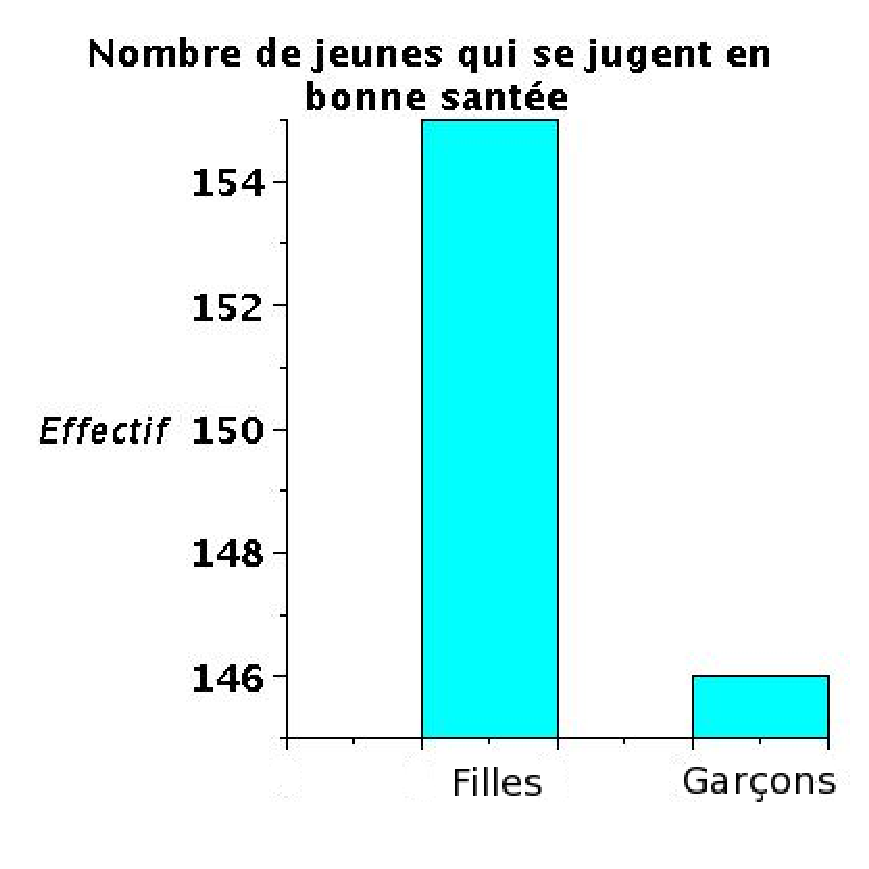
\includegraphics[width=6cm]{Q2053.eps}
 % Q2053.eps: 1179666x1179666 pixel, 0dpi, infxinf cm, bb=
\end{center}
Peut-on se fier \`a la conclusion apport\'ee? Oui ou non?\\

R\'eponse : Non\\

R\'etroaction :\\
Si on regarde l'\'echelle de l'axe des ordonn\'ees du graphique, on peut remarquer qu'il y a une coupure. Il y a donc 155 filles qui se consid\`erent en sant\'e contre 146 gar\c cons. On ne peut donc pas conclure que les filles se consid\`erent beaucoup plus en forme que les gar\c cons.\\
Par cons\'equent, la r\'eponse est: non.\\

%Quartiles

2054-- Pour la distribution suivante, calculer l'\'etendue interquartile.
\begin{center}
 \begin{tabular}{|c  c  c  c  c|} \hline

23 & 24 & 24 & 25 & 30\\
32 & 36 & 37 & 37 & 39 \\
41 & 51 & 52 & 54 & 55 \\ \hline

\end{tabular}
\end{center}

R\'eponse : 26\\

R\'etroaction :
\begin{center}
 \begin{tabular}{|c  c  c  c  c|} \hline

23 & 24 & 24 & 25 & 30\\
32 & 36 & 37 & 37 & 39 \\
41 & 51 & 52 & 54 & 55 \\ \hline

\end{tabular}
\end{center}
Pour calculer l'\'etendue interquartile, il faut conna\^itre le premier et le troisi\`eme quartile. Comme il y a 15 donn\'ees, le premier quartile est la quatri\`eme donn\'ee, soit 25.\\
Le troisi\`eme quartile est la douzi\`eme donn\'ee, soit 51.\\
Enfin, on calcule la distance entre ces deux nombres:\\
\begin{equation*}
 51-25=26
\end{equation*}
Par cons\'equent, la r\'eponse est 26.\\

2055-- Pour la distribution suivante, calculer l'\'etendue interquartile.
\begin{center}
 \begin{tabular}{|c  c  c  c  c  c |} \hline

2 & 2 & 2 & 2 & 3 & 3 \\
3 & 3 & 3 & 3 & 3 & 4 \\
4 & 5 & 5 & 5 & 5 & 6 \\ \hline

\end{tabular}
\end{center}

R\'eponse : 2\\

R\'etroaction :
\begin{center}
 \begin{tabular}{|c  c  c  c  c  c |} \hline

2 & 2 & 2 & 2 & 3 & 3 \\
3 & 3 & 3 & 3 & 3 & 4 \\
4 & 5 & 5 & 5 & 5 & 6 \\ \hline

\end{tabular}
\end{center}
Pour calculer l'\'etendue interquartile, il faut conna\^itre le premier et le troisi\`eme quartile. Comme il y a 18 donn\'ees, le premier quartile est la cinqui\`eme donn\'ee.\\
Le premier quartile vaut donc 3.\\
Le troisi\`eme quartile est la 14\ieme{} donn\'ee.\\
Le troisi\`eme quartile vaut donc 5.\\
Enfin on cacule la distance entre ces deux nombres:\\
\begin{equation*}
 5-3=2
\end{equation*}
Par cons\'equent, la r\'eponse est 2.\\



%Mesures de position

2056-- Le professeur de Laurence lui dit que sa note au dernier examen lui a permis d'obtenir un rang centile de 48.  Voici les notes des \'el\`eves de la classe.
\begin{quote}
12, 12, 13, 15, 16, 17, 17, 18, 18, 18, 19, 20, 20, 20, 21, 24, 24, 24, 25, 27, 29, 29, 30
\end{quote}
Quel est la note de Laurence? \\

R\'eponse : 19\\

R\'etroaction :\\
Pour trouver la note de Laurence, il faut calculer combien de notes sont \'egales ou inf\'erieures \`a sa note.\\
\begin{equation*}
 \frac{48}{100}\times 23 \approx 11,04
\end{equation*}
Comme la r\'eponse n'est pas un entier, il faut arrondir. On a donc que 11 \'el\`eves on eu une note \'egale ou inf\'erieure \`a celle de Laurence. On trouve que sa note est 19.\\
Par cons\'equent, la r\'eponse est 19.\\

2057-- Lors de la course annuelle de la ville d'Antony, 10 coureurs se sont lanc\'es comme d\'efi de courir un marathon. Quel est le rang centile du coureur arriv\'e troisi\`eme au fil d'arriv\'e?\\

a$)$ 30\\
b$)$ 40\\
c$)$ 70\\
d$)$ 80\\

R\'eponse : d$)$\\

R\'etroaction :\\
Pour trouver le rang centile du coureur, il faut calculer combien de coureurs ont fait un temps inf\'erieur ou \'egal \`a son temps. \\
\begin{equation*}
 \frac{8}{10}\times 100 = 80
\end{equation*}
On trouve que son rang est 80.\\
Par cons\'equent, la r\'eponse est d).\\

%Interpretation des donnee

2058-- Jean-Fran\c cois travaille dans une boutique de v\^etements pour hommes. \`A la fin de sa journ\'ee, il regarde les montants des ventes de la journ\'ee. Il les entre dans un logiciel et fait imprimer des graphiques \`a partir des donn\'ees. Voici les grapiques imprim\'es. Lequel est le plus adapt\'e \`a la situation?\\

\begin{tabular}{l l}
a$)$ & b$)$ \\
 \includegraphics[width=7cm,height=8cm]{Q2058.eps}
 % Q2058.eps: 1179666x1179666 pixel, 0dpi, infxinf cm, bb=
&
 \includegraphics[width=7cm,height=8cm]{Q2058b.eps}
 % Q2058b.eps: 1179666x1179666 pixel, 0dpi, infxinf cm, bb=
\\
c$)$ & d$)$ \\
 \includegraphics[width=6cm,height=7cm]{Q2058c.eps}
 % Q2058b.eps: 1179666x1179666 pixel, 0dpi, infxinf cm, bb=
&
\includegraphics[width=6cm,height=7cm]{Q2058d.eps}\\
 % Q2058b.eps: 1179666x1179666 pixel, 0dpi, infxinf cm, bb=

\end{tabular}\\

R\'eponse : d$)$\\

R\'etroaction :\\
Le graphique le plus appropri\'e \`a cette situation est le diagramme de quartiles, car il permet de voir en un coup d'oeil comment ont \'et\'e les ventes de la journ\'ee. Les autres graphiques ne font qu'afficher la valeur de chaque vente ou leur valeur relative.\\
Par cons\'equent, la r\'eponse est d).\\

2059-- Voici les notes au dernier test de musique de la classe de
John.
\begin{quote}
 70, 70, 72, 75, 75, 80, 83, 84, 86, 87, 87, 89, 92, 92, 92
\end{quote}
Quelle est le rang cinqui\`eme de l'\'el\`eve qui a obtenu une note de 80? \\

a$)$ Premier rang cinqui\`eme.\\
b$)$ Deuxi\`eme rang cinqui\`eme. \\
c$)$ Troisi\`eme rang cinqui\`eme.\\
d$)$ Quatri\`eme rang cinqui\`eme.\\

R\'eponse : d$)$\\

R\'etroaction :\\
\begin{itemize}
 \item Le premier rang cinqui\`eme contient les trois notes de 92. \\
\item Le deuxi\`eme rang cinqui\`eme contient les notes 87 et 89.\\
\item Le troisi\`eme rang cinqui\`eme contient les notes 83, 84 et 86. \\
\item Le quatri\`eme rang cinqui\`eme contient les notes 75 et 80.\\
\end{itemize}
Par cons\'equent, la r\'eponse est d).\\

2060-- Dans une relation de variation directe, le taux de variation est \underline{\qquad\qquad}. \\

a$)$ constant \\
b$)$ directement proportionnel\\
c$)$ nul\\
d$)$ toujours 1\\

R\'eponse : a$)$ \\

R\'etroaction :\\
Dans une relation de variation directe, le taux de variation est \underline{\textbf{constant}}.\\
Par cons\'equent, la r\'eponse est a).\\
Le graphique suivant est un exemple de relation de variation directe.\\
\begin{center}
 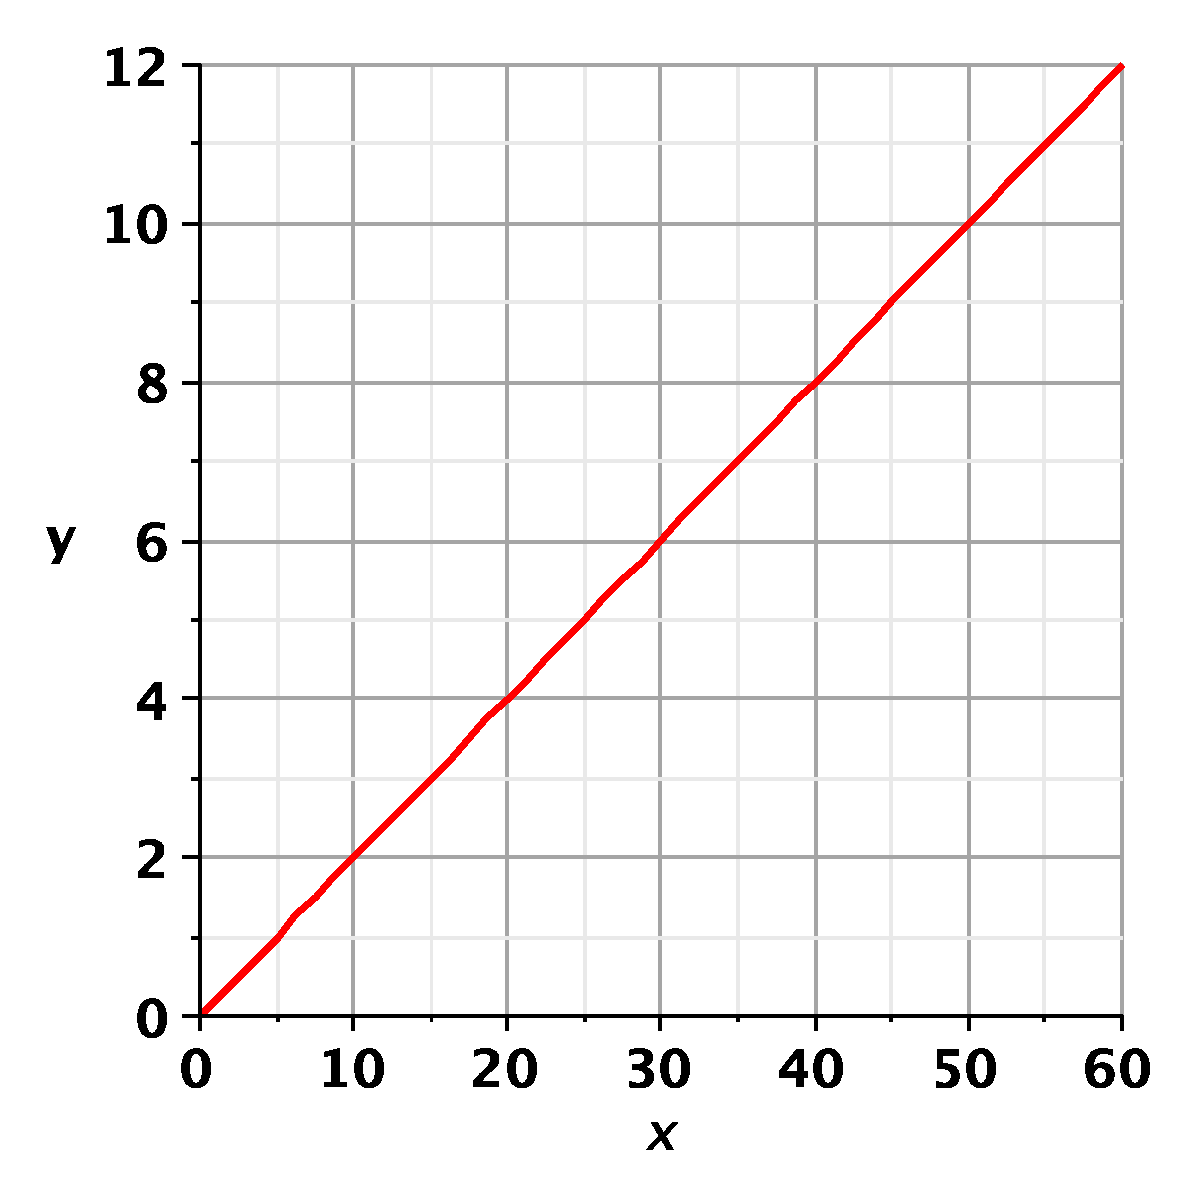
\includegraphics[width=6cm,bb=20 118 575 673]{Q2064.eps}
 % Q2064.eps: 1179666x1179666 pixel, 300dpi, 9987.84x9987.84 cm, bb=20 118 575 673
\end{center}

2061-- Jo\"{e}lle a 15 ans. Elle veut s'abonner \`a la revue hebdomadaire \og L'actu \fg. L'abonnement co\^ute 12,50\$ par mois. Elle a 100\$ en poche. Elle d\'ecide de faire une table de valeurs pour conna\^itre le nombre de mois auxquels elle peut s'abonner. \\
Quelles sont les variables d\'ependante et ind\'ependante de cette situation?\\

\begin{tabular}{l l l}
a$)$ & Variable d\'ependante: l'\^age de Jo\"{e}lle & Variable ind\'ependante: le co\^ut de l'abonnement\\
b$)$ & Variable d\'ependante: le co\^ut d'une revue & Variable ind\'ependante: le nombre de mois\\
c$)$ & Variable d\'ependante: le co\^ut de l'abonnement & Variable ind\'ependante: le nombre de mois\\
d$)$ & Variable d\'ependante: le nombre de mois & Variable ind\'ependante: le co\^ut de l'abonnement\\
\end{tabular}\\
\\
R\'eponse : c$)$ \\

R\'etroaction :\\
La variable d\'ependante de cette situation est le co\^ut de l'abonnement et la variable ind\'ependante est le nombre de mois. En effet, le co\^ut de l'abonnement d\'epend du nombre de mois auxquels elle d\'ecide de s'abonner.\\
Par cons\'equent, la r\'eponse est c).\\

2062-- Une table de valeurs associ\'ee \`a une fonction permet de calculer rapidement diff\'erentes valeurs. Parmi ces choix, quelles valeurs peut-on calculer?\\

1. Le taux de variation\\
2. La variation de la variable ind\'ependante\\
3. La valeur initiale\\

a$)$  1 et 2\\
b$)$  1 et 3\\
c$)$  1, 2 et 3\\
d$)$  2 et 3\\

R\'eponse : c$)$\\

R\'etroaction :\\
Une table de valeurs permet de calculer rapidement diff\'erentes valeurs comme le taux de variation, la variation des variables et la valeur initiale d'une fonction.\\
\begin{itemize}
 \item Le taux de variation est la variation de la variable d\'ependante divis\'e par la variation de la variable ind\'ependante.
\item La variation de la variable ind\'ependante est la diff\'erence entre deux valeurs cons\'ecutives de la variable ind\'ependante.
\item La valeur initiale est la valeur de la variable d\'ependante lorsque la variable ind\'ependante vaut z\'ero.
\end{itemize}
Par cons\'equent, la r\'eponse est c$)$.\\

2063--  Luc veut s'abonner \`a la revue mensuelle \og M\'ecanique automobile \fg. L'abonnement co\^ute 17,50\$ par mois. Luc a 130\$ en poche. Il d\'ecide de faire une table de valeurs pour conna\^itre le nombre de mois auxquels il peut s'abonner. \\
Quelle table repr\'esente la situation?\\

\begin{tabular}{rlrl}
a$)$ &
\begin{tabular}{|c|c|} \hline
{\bf Nombre de mois } & {\bf Co\^ut (en \$)}  \\ \hline \hline
1 & 17,50 \\ \hline
2 & 35 \\ \hline
3 & 52,50 \\ \hline
4 & 70 \\ \hline
$\ldots$ & $\ldots$ \\ \hline
\multicolumn{2}{c}{}\\
\end{tabular}
& b$)$ &
\begin{tabular}{|c|c|} \hline
{\bf Nombre de mois} & {\bf Co\^ut (en \$)}  \\ \hline \hline
0 & 0 \\ \hline
1 & $-17,50$ \\ \hline
2 & $-35$ \\ \hline
3 & $-52,50$ \\ \hline
$\ldots$ & $\ldots$ \\ \hline
\multicolumn{2}{c}{}\\
\end{tabular}
\\
c$)$ &
\begin{tabular}{|c|c|} \hline
{\bf Nombre de mois} & {\bf Co\^ut (en \$)}  \\ \hline \hline
1 & 17,50 \\ \hline
2 & 17,50 \\ \hline
3 & 17,50 \\ \hline
4 & 17,50 \\ \hline
$\ldots$ & $\ldots$ \\ \hline
\multicolumn{2}{c}{}\\
\end{tabular}
& d$)$ &
\begin{tabular}{|c|c|} \hline
{\bf Nombre de mois} & {\bf Co\^ut (en \$)}  \\ \hline \hline
1 & 130 \\ \hline
2 & 112,50 \\ \hline
3 & 95 \\ \hline
4 & 77,50 \\ \hline
$\ldots$ & $\ldots$ \\ \hline
\multicolumn{2}{c}{}\\
\end{tabular}
\end{tabular}\\


R\'eponse : a$)$\\

R\'etroaction :\\
\begin{center}
 \begin{tabular}{|c|c|} \hline
{\bf Nombre de mois } & {\bf Co\^ut (en \$)}  \\ \hline \hline
1 & 17,50 \\ \hline
2 & 35 \\ \hline
3 & 52,50 \\ \hline
4 & 70 \\ \hline
$\ldots$ & $\ldots$ \\ \hline
\multicolumn{2}{c}{}\\
\end{tabular}
\end{center}
La table qui repr\'esente la situation est la table a). On peut y voir l'augmentation du co\^ut de l'abonnement selon le nombre de mois auxquels Luc est abonn\'e \`a la revue.\\
Par cons\'equent, la r\'eponse est a$)$.\\

2064-- Une relation qui poss\`ede un taux de variation constant et une valeur initiale diff\'erente de z\'ero est \underline{\qquad\qquad}. \\

a$)$ une relation constante\\
b$)$ une relation de fonction\\
c$)$ une relation de variation partielle \\
d$)$ une relation lin\'eaire non nulle\\

R\'eponse : c$)$\\

R\'etroaction :\\
Une relation qui poss\`ede un taux de variation constant et une valeur initiale diff\'erente de z\'ero est une relation de variation partielle. \\
Par cons\'equent, la r\'eponse est c$)$.\\
Le graphique suivant est un exemple d'une relation de variation partielle.\\
\begin{center}
 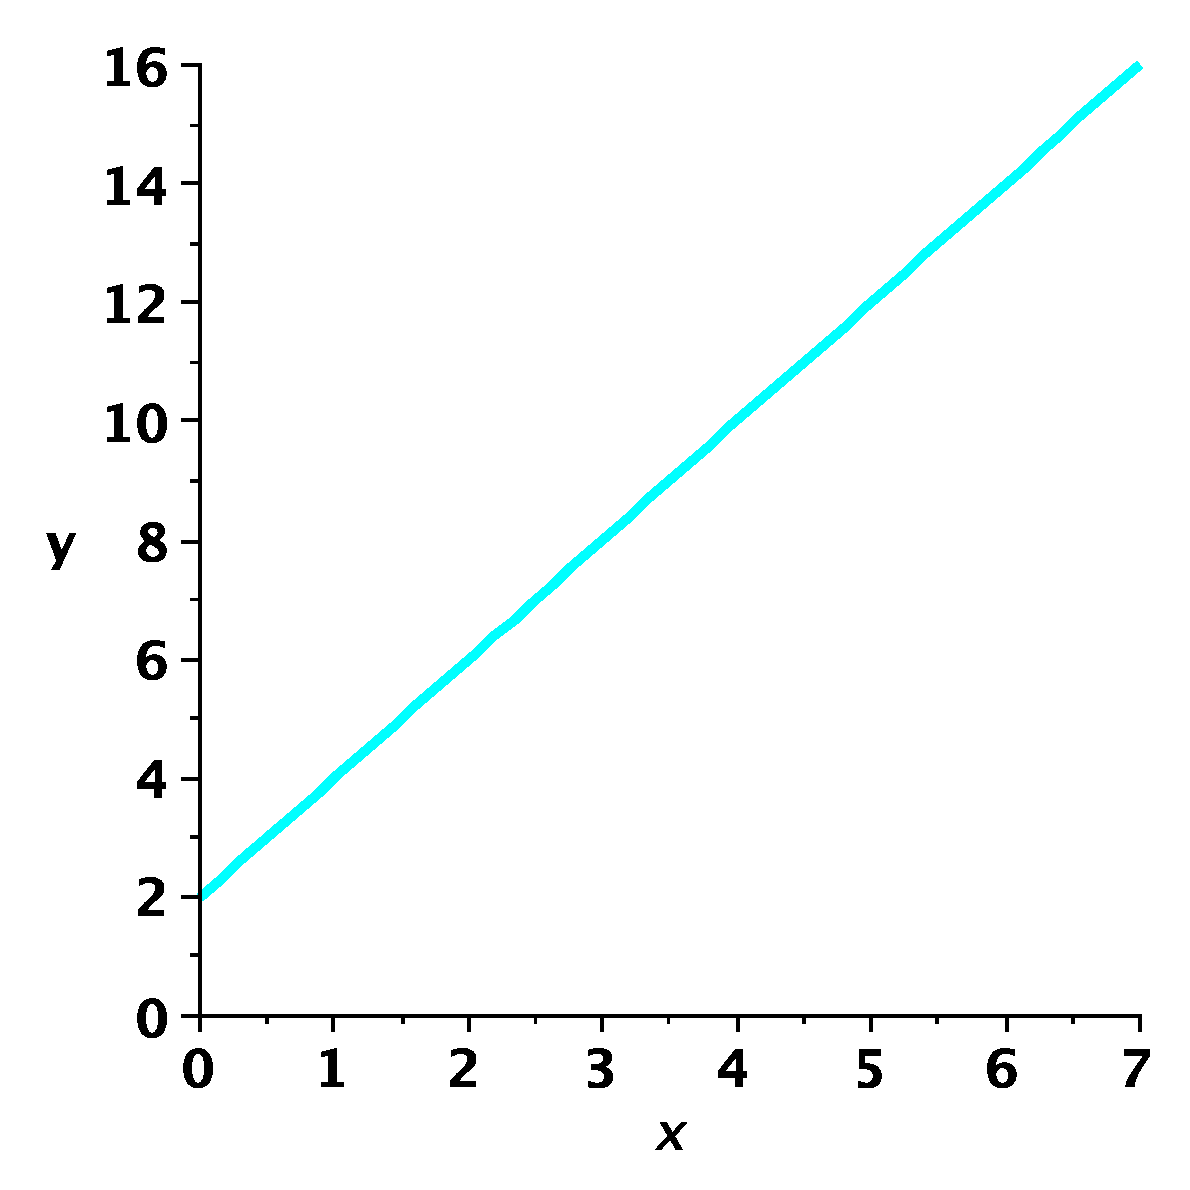
\includegraphics[width=6cm,bb=20 118 575 673]{Q2060.eps}
 % Q2060.eps: 3080293x7143525 pixel, 300dpi, 26079.81x60481.84 cm, bb=20 118 575 673
\end{center}

2065-- Louis mesure la capacit\'e de bo\^ites d'entreposage. Les bo\^ites ont toutes la m\^eme hauteur de \mbox{30 cm} et ce n'est que la dimension du fond, en forme de carr\'e, qui varie. Voici le tableau de la capacit\'e des bo\^ites selon la longueur d'une ar\^ete du fond.
\begin{center}
 \begin{tabular}{|c|c|} \hline
{\bf Mesure de l'ar\^ete (en dm)} & {\bf Capacit\'e (en dm$^{3}$)}  \\ \hline \hline
1 & 3 \\ \hline
2 & 12 \\ \hline
3 & 27 \\ \hline
4 & 48 \\ \hline
$\ldots$ & $\ldots$ \\ \hline
\multicolumn{2}{c}{}\\
\end{tabular}
\end{center}
Louis d\'esire faire un graphique repr\'esentant la capacit\'e d'une bo\^ite selon la longueur de ses ar\^etes. Il d\'ecide de faire varier les valeurs sur l'axe des abscisses de 0 \`a 5 dm, avec un pas de 1 dm entre chaque graduation. Quel est le meilleur choix de graduation de l'axe des ordonn\'ees?\\

a$)$ Une variation de 0 \`a 75 et un pas de 1 dm. \\
b$)$ Une variation de 0 \`a 75 et un pas de 15 dm. \\
c$)$ Une variation de 3 \`a 48 et un pas de 1 dm. \\
d$)$ Une variation de 3 \`a 48 et un pas de 15 dm. \\

R\'eponse : b$)$\\

R\'etroaction :\\
\begin{center}
 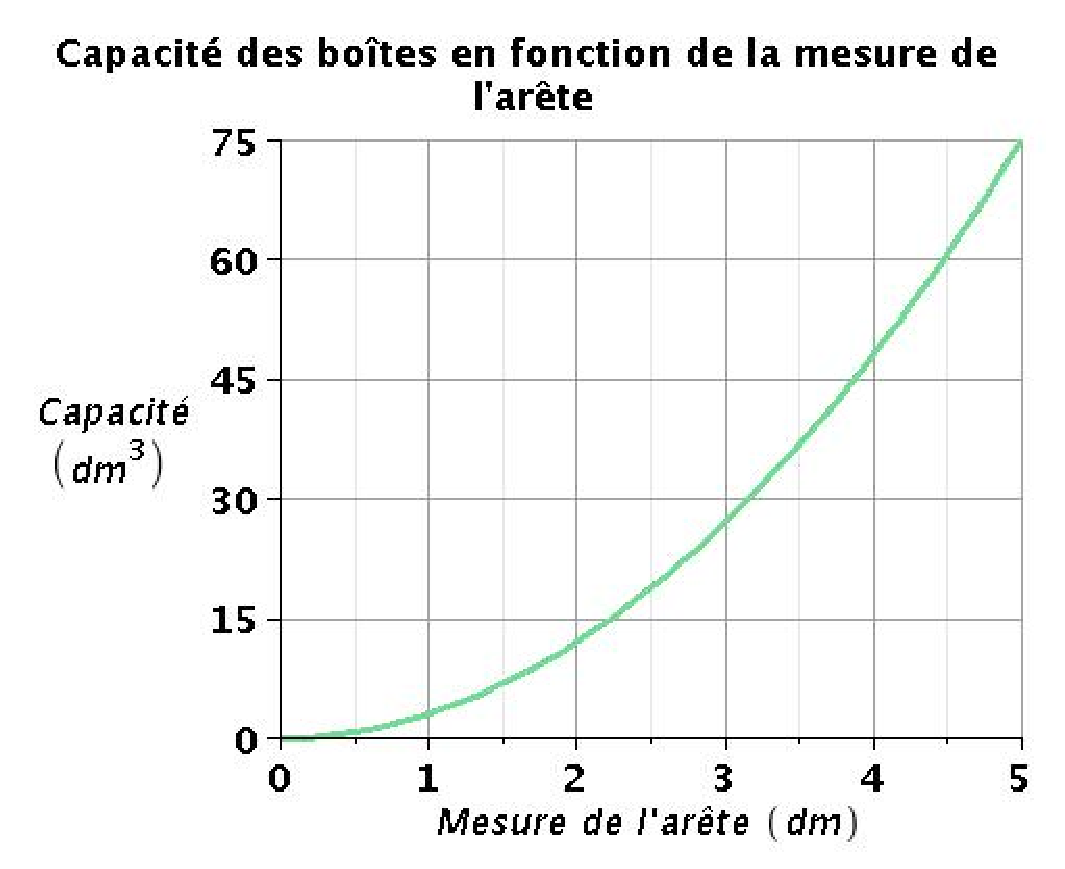
\includegraphics[width=8cm,bb=14 14 509 415]{Q2065.eps}
 % Q2065.eps: 1179666x1179666 pixel, 300dpi, 9987.84x9987.84 cm, bb=14 14 509 415
\end{center}
Pour graduer l'axe des ordonnn\'ees, le meilleur choix est de prendre une variation de 0 \`a 75 avec un pas de 15 dm. Ainsi, on a cinq graduations qui nous permettent de faire une approximation de l'allure de notre graphique.\\
Par cons\'equent, la r\'eponse est b$)$.\\

2066-- Pour quelles fonctions le taux de variation n'est-il pas constant?\\

1. Relation de variation directe\\
2. Relation de variation du second degr\'e\\
3. Relation de variation inverse\\
4. Relation de variation partielle\\

a$)$ 1 et 2\\
b$)$ 1 et 4\\
c$)$ 2 et 3\\
d$)$ 3 et 4\\

R\'eponse : c$)$\\

R\'etroaction :\\
\begin{itemize}
 \item Dans une fonction de variation directe ou partielle, le taux de variation est toujours constant.\\
\begin{center}
 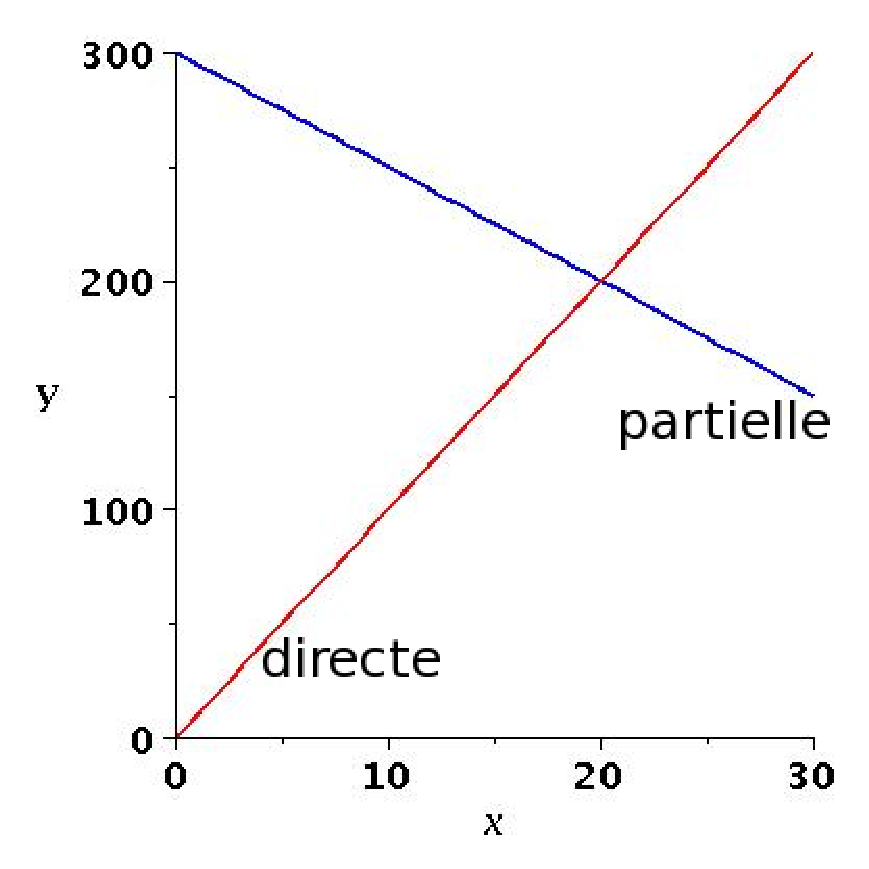
\includegraphics[width=6cm,bb=14 14 415 415]{Q2066a.eps}
 % Q2066a.eps: 1179666x1179666 pixel, 300dpi, 9987.84x9987.84 cm, bb=14 14 415 415
\end{center}
 \item Dans une fonction de variation directe du second degr\'e ou inverse, le taux de variation n'est pas constant.\\
\begin{center}
 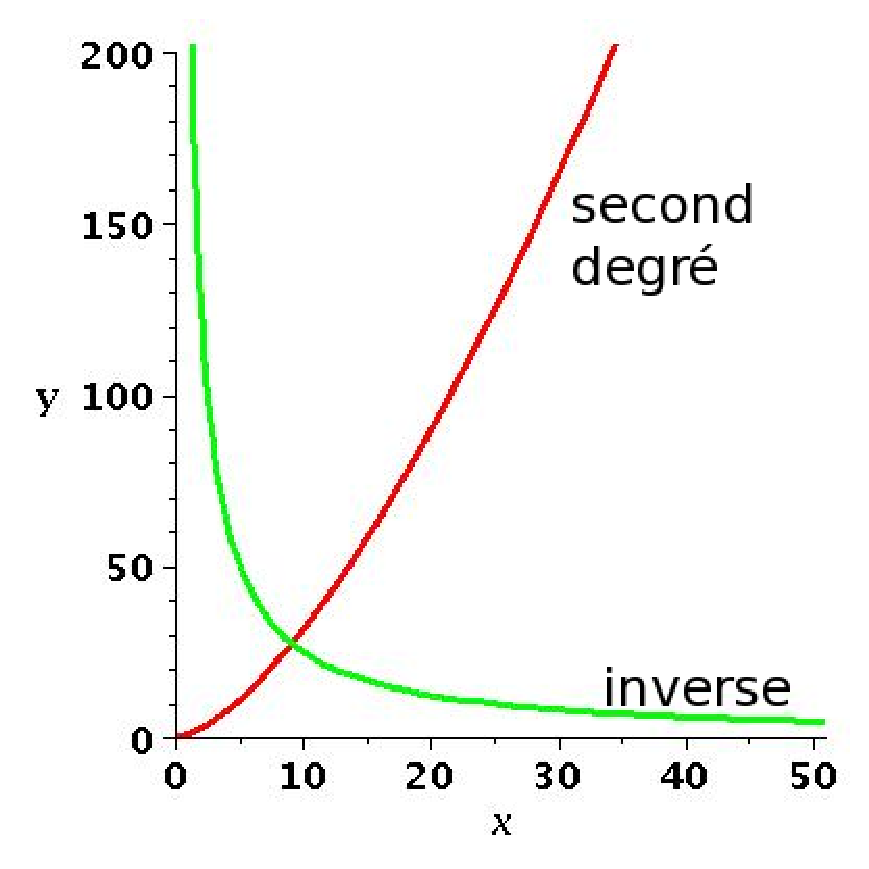
\includegraphics[width=6cm,bb=14 14 415 415]{Q2066b.eps}
 % Q2066b.eps: 1179666x1179666 pixel, 300dpi, 9987.84x9987.84 cm, bb=14 14 415 415
\end{center}
\end{itemize}
Par cons\'equent, la r\'eponse est c).\\

2067-- Daniella mesure la capacit\'e de diff\'erentes bo\^ites. Les bo\^ites ont toutes la m\^eme hauteur de \mbox{30 cm} et ce n'est que la dimension du fond, en forme de carr\'e, qui varie. Voici le tableau de la capacit\'e des bo\^ites selon la longueur d'une ar\^ete du fond.
\begin{center}
 \begin{tabular}{|c|c|} \hline
{\bf Mesure de l'ar\^ete (en dm)} & {\bf Capacit\'e (en dm$^{3}$)}\\ \hline \hline
1 & 3 \\ \hline
2 & 12 \\ \hline
3 & 27 \\ \hline
4 & 48 \\ \hline
$\ldots$ & $\ldots$ \\ \hline
\multicolumn{2}{c}{}\\
\end{tabular}
\end{center}
Quelle est l'\'equation de cette fonction?\\

a$)$ $y = x^{2} + 3$\\
b$)$ $y = x^{3}$ \\
c$)$ $y = 3x^{2}$\\
d$)$ $y = 30x^{2}$\\

R\'eponse : c$)$\\

R\'etroaction :\\
Pour calculer la capacit\'e d'une bo\^ite, il faut mettre au carr\'e la longueur de l'ar\^ete du fond puis multiplier par la hauteur de la bo\^ite qui mesure 3 dm. Il faut faire attention d'utiliser les m\^emes unit\'es de mesure : 10 cm = 1 dm.
\begin{eqnarray*}
 \textrm{capacit\'e} &=& 3 \times \textrm{longueur de l'ar\^ete}^{2}\\
  y &=& 3 \times x^{2}
\end{eqnarray*}
Par cons\'equent, la r\'eponse est c).\\


2068-- Quelle est la forme d'une \'equation de variation inverse? \\

a$)$ variable d\'ependante = $\frac{\textrm{constante}}{\textrm{variable ind\'ependante}}$\\ [2mm]
b$)$ variable d\'ependante = $\frac{\textrm{variable ind\'ependante}}{\textrm{constante }}$\\ [2mm]
c$)$ variable d\'ependante = $ a \times \textrm{variable ind\'ependante} + b $\\ [2mm]
d$)$ variable d\'ependante = $ a \times \textrm{variable ind\'ependante}^{2} + b $\\ [2mm]

R\'eponse : a$)$\\

R\'etroaction :\\
Dans une relation de variation inverse, l'\'equation prend cette forme: \\
\begin{equation*}
\textrm{variable d\'ependante} = \frac{\textrm{constante}}{\textrm{variable ind\'ependante}}\\
\end{equation*}
Voici un graphique repr\'esentant une fonction de variation inverse.
\begin{center}
 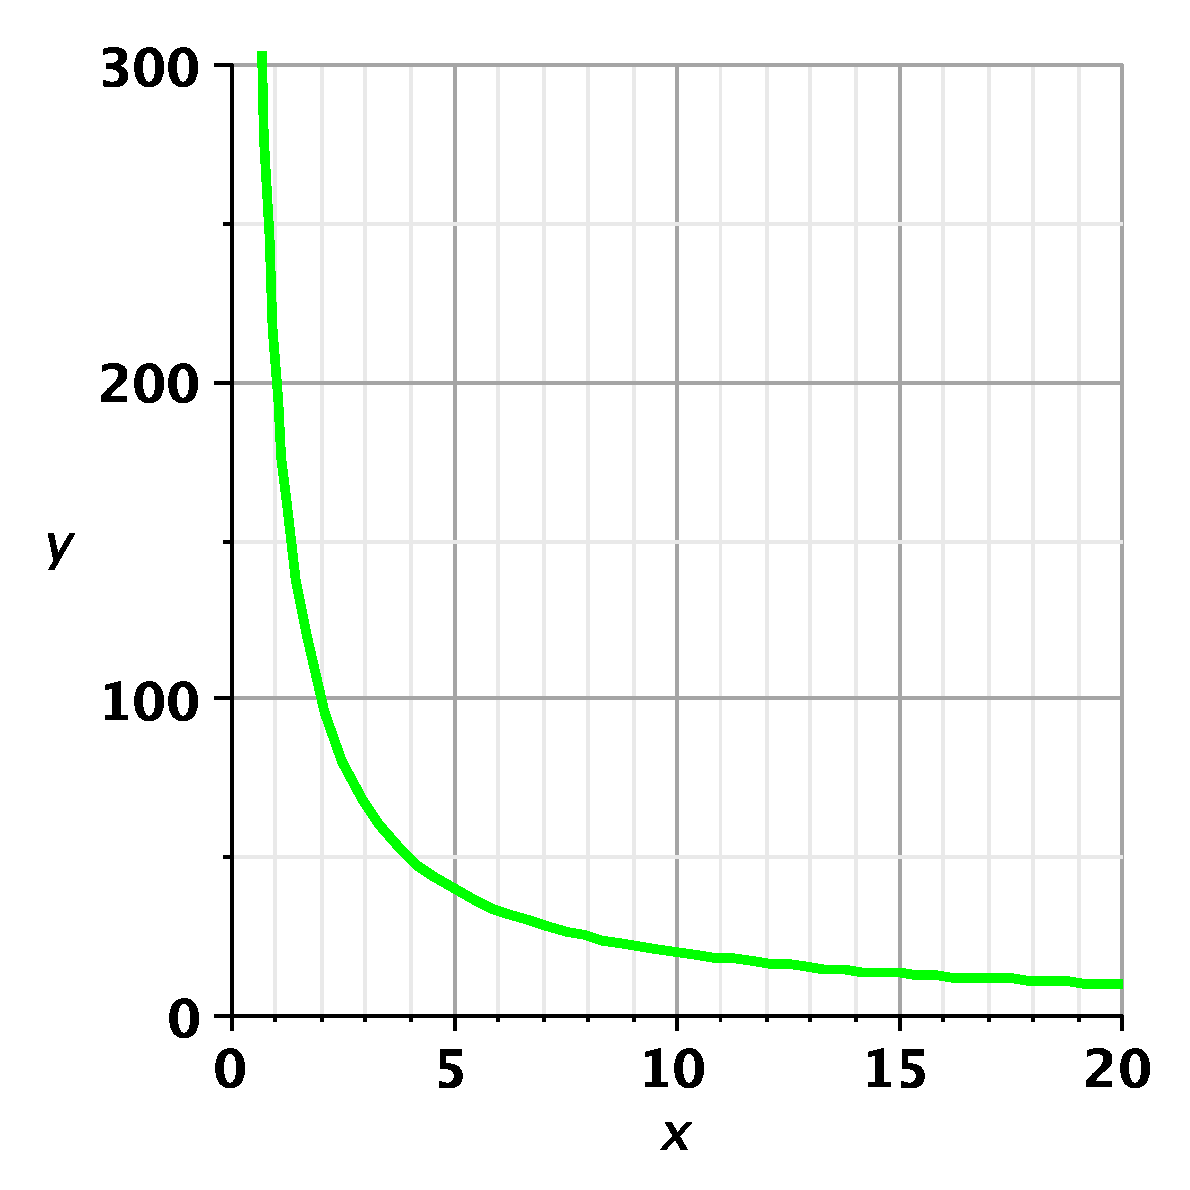
\includegraphics[width=6cm,bb=20 118 575 673]{Q2068.eps}
 % Q2068.eps: 1179666x1179666 pixel, 300dpi, 9987.84x9987.84 cm, bb=20 118 575 673
\end{center}
Par cons\'equent, la r\'eponse est a).\\

2069-- Voici le graphique repr\'esentant le salaire horaire des employ\'es des entreprises A (en rouge) et B (en bleu).
\begin{center}
 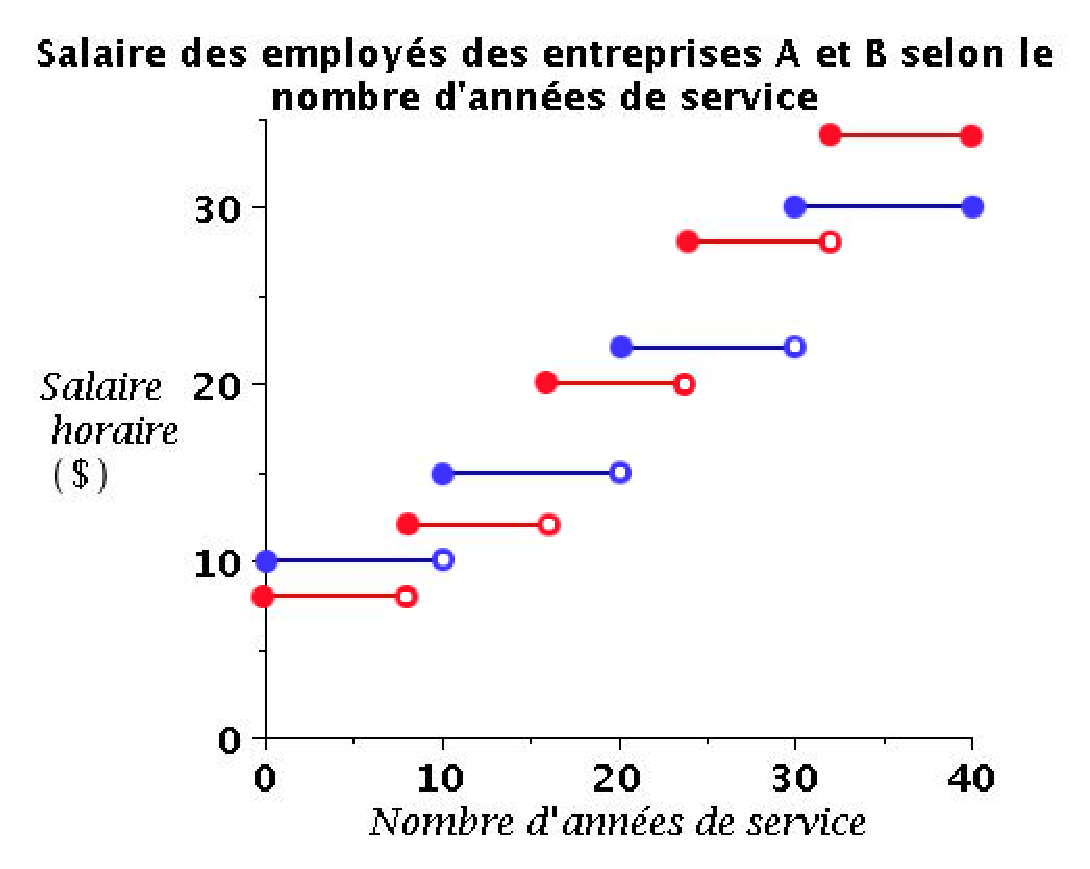
\includegraphics[width=8cm]{Q2069.eps}
 % Q2069.eps: 1179666x1179666 pixel, 300dpi, 9987.84x9987.84 cm, bb=14 14 415 415
\end{center}
Julie-Ann dit qu'il est plus payant de travailler dans l'entreprise B lorsqu'on a 20 ans de service.\\
Est-ce vrai ou faux?\\

R\'eponse : vrai\\

R\'etroaction :
\begin{center}
 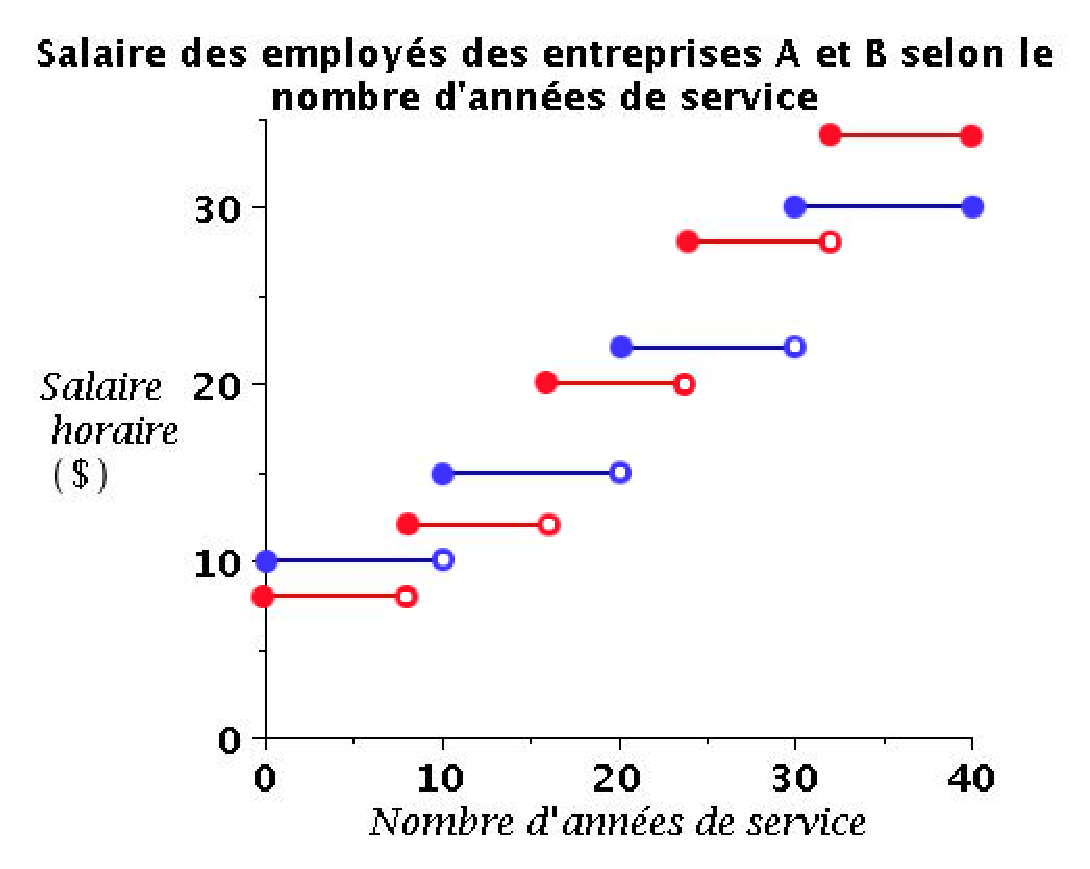
\includegraphics[width=8cm]{Q2069.eps}
 % Q2069.eps: 1179666x1179666 pixel, 300dpi, 9987.84x9987.84 cm, bb=14 14 415 415
\end{center}
Lorsqu'un employ\'e de l'entreprise B a 20 ans de service, son salaire augmente \`a plus de 20\$ de l'heure alors que dans l'entreprise A son salaire est de 20\$ de l'heure.\\
Par cons\'equent, la r\'eponse est: vrai.\\

%Questions sur les fonctions mathematiques 416 difficulte 2

2070-- Voici l'\'equation d'une fonction de variation partielle et le graphique sur lequel on d\'esire tracer la fonction. Quelle est sa variable ind\'ependante et sa variable d\'ependante? \\
\begin{equation*}
 m = 2n + 3
\end{equation*}
\begin{center}
 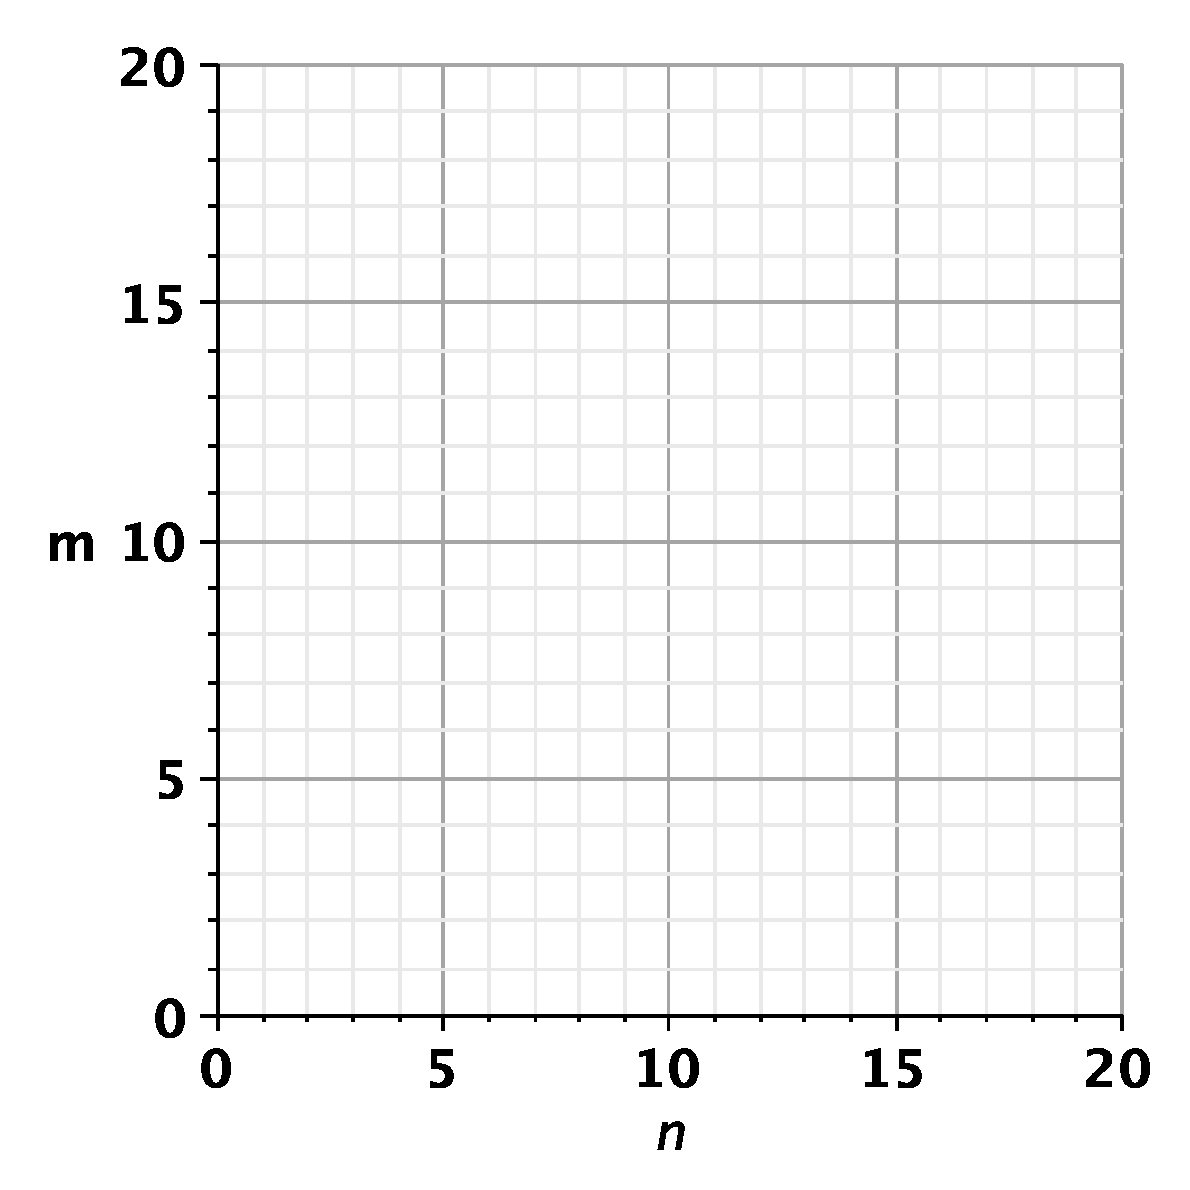
\includegraphics[width=5cm,bb=20 118 575 673]{Q2070.eps}
 % Q2070.eps: 1179666x1179666 pixel, 300dpi, 9987.84x9987.84 cm, bb=20 118 575 673
\end{center}

a$)$ sa variable ind\'ependante est $m$ et sa variable d\'ependante est $n$ \\
b$)$ sa variable ind\'ependante est $n$ et sa variable d\'ependante est $m$ \\
c$)$ sa variable ind\'ependante est $n$ et sa variable d\'ependante est 3 \\
d$)$ sa variable ind\'ependante est 3 et sa variable d\'ependante est $n$ \\

R\'eponse : b$)$\\

R\'etroaction :\\
Dans cette \'equation de fonction de variation partielle, la variable ind\'ependante est $n$ et la variable d\'ependante est $m$. \\
\begin{equation*}
 m = 2n + 3
\end{equation*}
Par cons\'equent, la r\'eponse est b).\\

2071-- Voici un graphique repr\'esentant une situation. Quel sc\'enario propos\'e est le plus plausible?
\begin{center}
 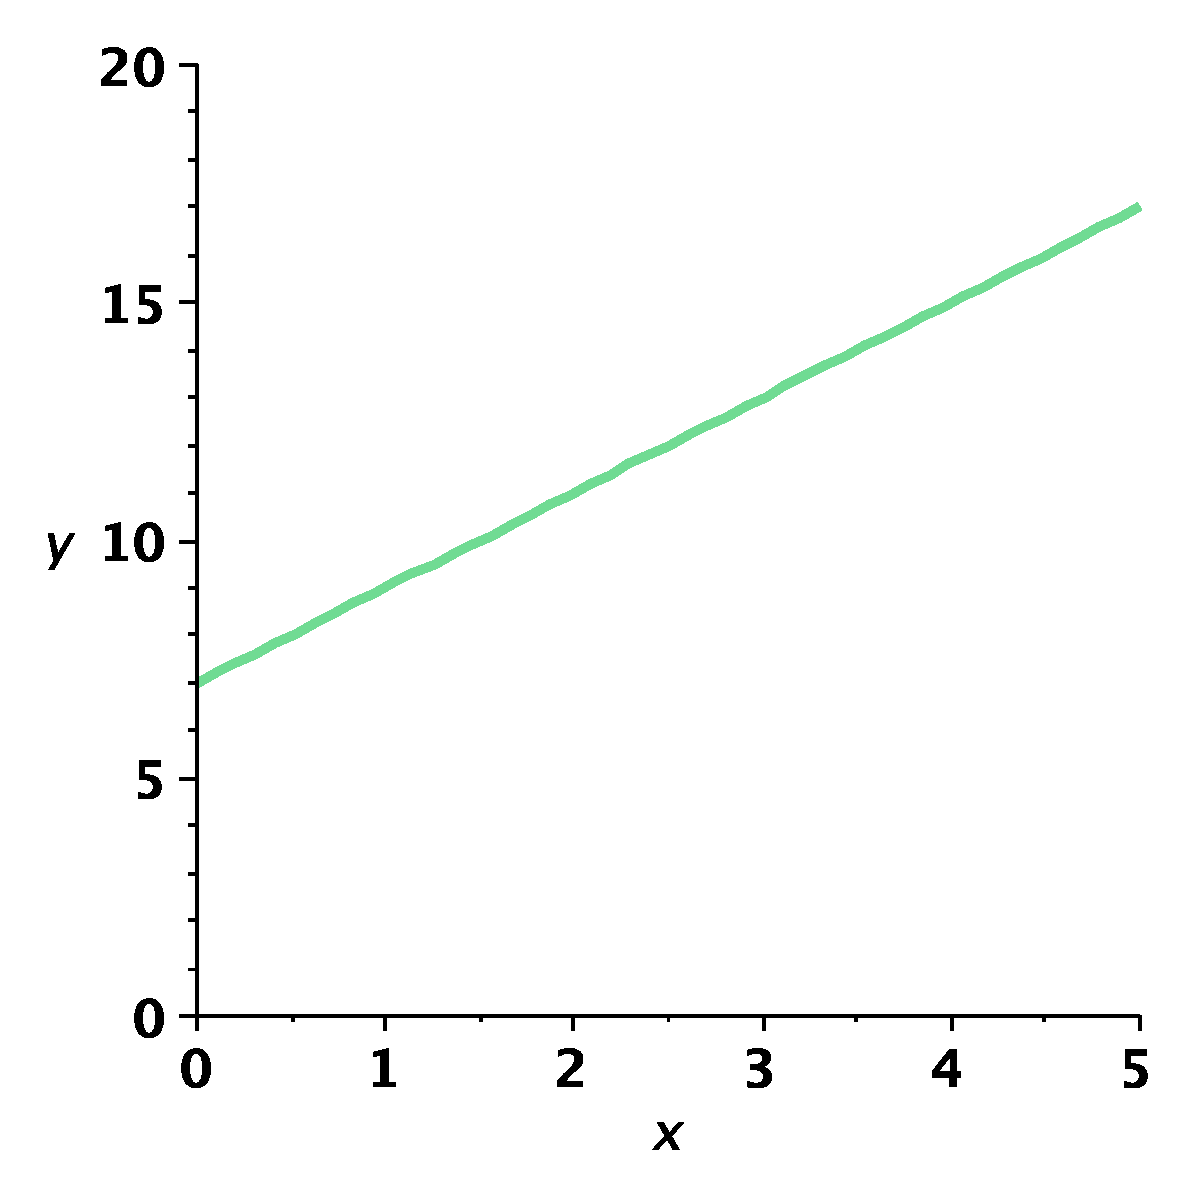
\includegraphics[width=6cm]{Q2071.eps}
 % Q2071.eps: 0x0 pixel, 300dpi, 0.00x0.00 cm, bb=20 118 575 673
\end{center}

a$)$ C'est la distance d'un randonneur \`a son point d'arriv\'ee selon le temps de marche.\\
b$)$ C'est la quantit\'e d'eau dans une piscine, lors de son remplissage, selon le temps.\\
c$)$ C'est la quantit\'e d'eau dans un bain apr\`es avoir enlev\'e le bouchon. \\
d$)$ C'est la vitesse de vol d'un oiseau selon le temps de vol.\\

R\'eponse : b$)$\\

R\'etroaction :\\
\begin{center}
 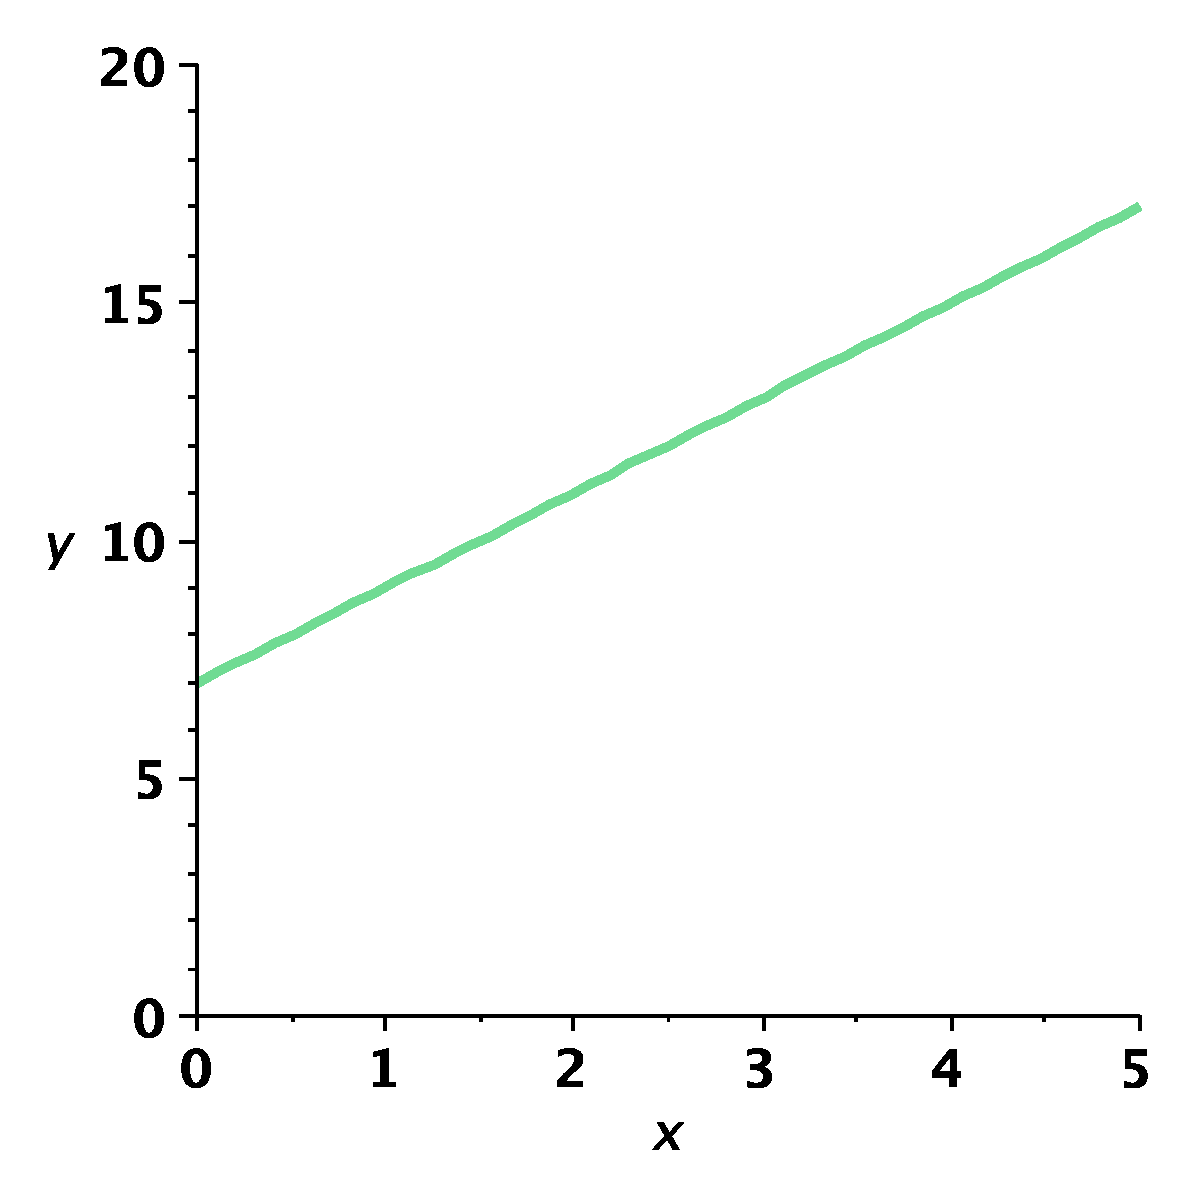
\includegraphics[width=6cm]{Q2071.eps}
 % Q2071.eps: 0x0 pixel, 300dpi, 0.00x0.00 cm, bb=20 118 575 673
\end{center}
Le sc\'enario propos\'e qui est le plus plausible est la quantit\'e d'eau dans une piscine, lors de son remplissage, selon le temps. On a une relation lin\'eaire de variation partielle qui nous permet de voir une augmentation constante de la valeur de $y$ lorsque $x$ augmente. \\
Par cons\'equent, la r\'eponse est b$)$.\\

2072-- Voici la table de valeurs d'une fonction de variation partielle.
\begin{center}
 \begin{tabular}{|c|c|} \hline
{\bf Abscisse ($x$)} & {\bf Ordonn\'ee ($y$)}  \\ \hline \hline
0 & 2 \\ \hline
1 & 3 \\ \hline
2 & 4 \\ \hline
3 & 5 \\ \hline
4 & 6 \\ \hline
$\ldots$ & $\ldots$ \\ \hline
\multicolumn{2}{c}{}\\
\end{tabular}
\end{center}
Quelle est la valeur initiale?\\

a$)$ 0\\
b$)$ 1\\
c$)$ 2\\
d$)$ 3\\

R\'eponse : c$)$\\

R\'etroaction :\\
\begin{center}
 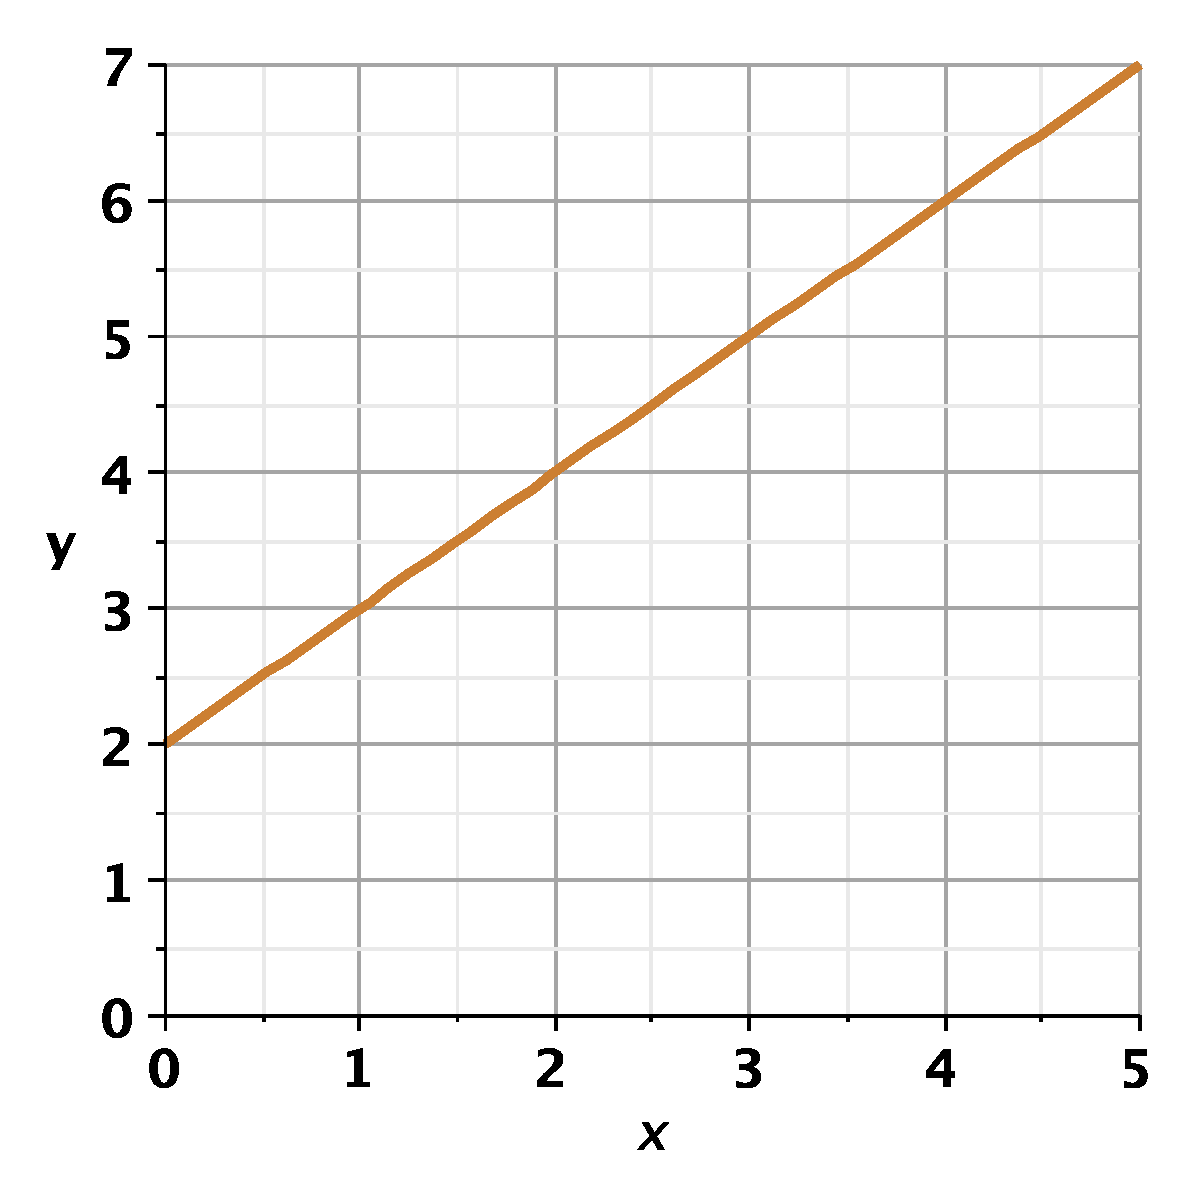
\includegraphics[width=6cm]{Q2072.eps}
 % Q2072.eps: 1179648x0 pixel, 300dpi, 9987.69x0.00 cm, bb=20 118 575 673
\end{center}
Dans une fonction de variation partielle, la valeur initiale, toujours diff\'erente de 0, est la valeur de la variable d\'ependante lorsque la variable ind\'ependante vaut 0. Comme on a le couple $(0,2)$ dans la table de valeurs, la valeur initiale est 2.\\
Par cons\'equent, la r\'eponse est c).\\

2073-- Voici le graphique d'une relation de variation en escalier. Compl\'eter la table de valeurs par les valeurs justes.
\begin{center}
 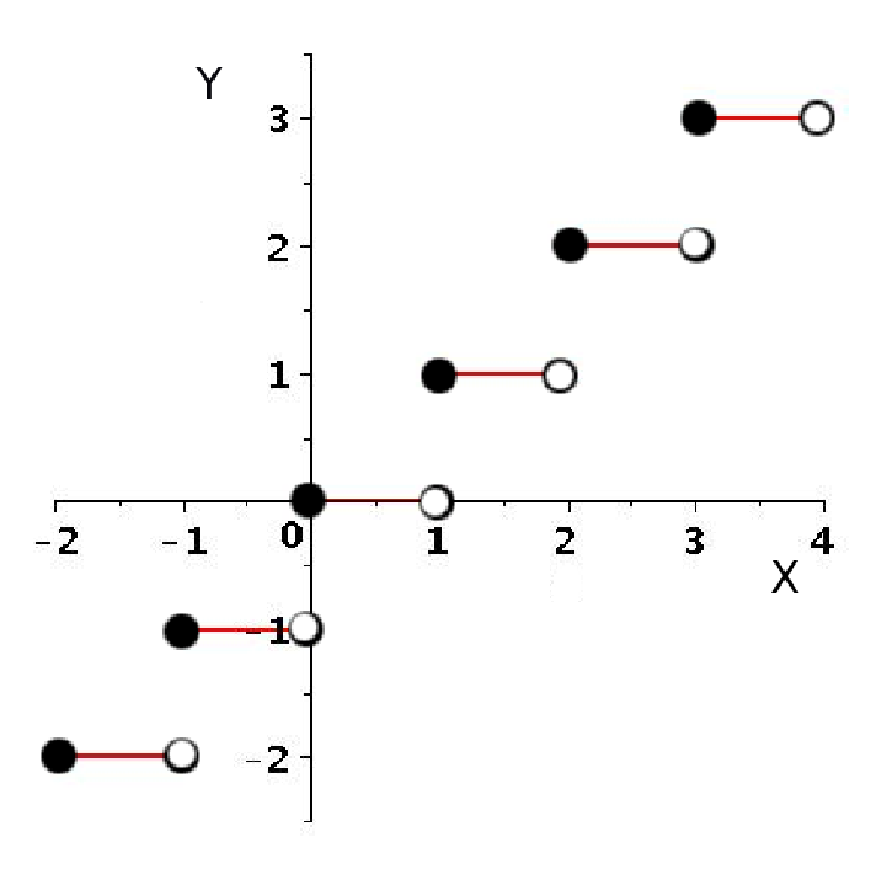
\includegraphics[width=6cm]{Q2073.eps}
 % Q2073.eps: 1179666x1179666 pixel, 300dpi, 9987.84x9987.84 cm, bb=14 14 415 415
\end{center}
\begin{center}
 \begin{tabular}{|c||c| c | c | c | c | c |} \hline
{\bf Abscisse ($x$)} & $-1,5$ & 0 & 0,5 & 2 & 2,9 & 3,5 \\ \hline \hline
{\bf Ordonn\'ee ($y$)} & $-2$ & A & 0 & B & C & 3 \\ \hline
\end{tabular}
\end{center}
a$)$ A = $-1$, B = 1 et C = 2.\\
b$)$ A = $-1$, B = 1 et C = 3.\\
c$)$ A = 0, B = 2 et C= 2.\\
d$)$ A = 0, B = 2 et C= 3.\\

R\'eponse : c$)$\\

R\'etroaction :\\
\begin{center}
 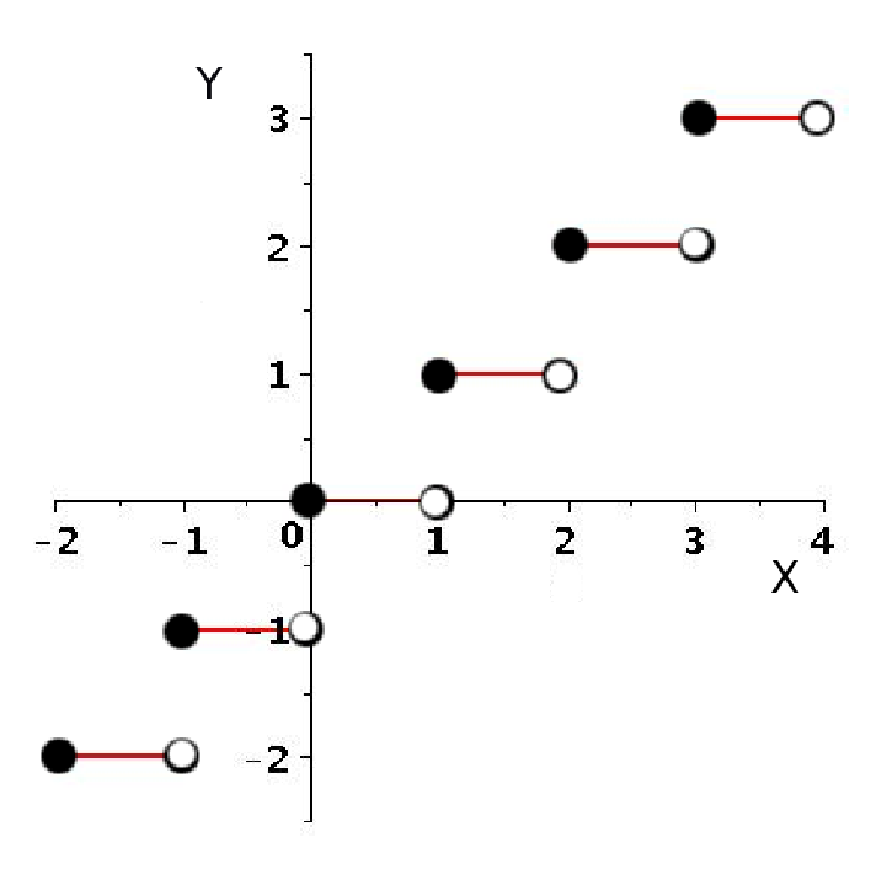
\includegraphics[width=6cm]{Q2073.eps}
 % Q2073.eps: 1179666x1179666 pixel, 300dpi, 9987.84x9987.84 cm, bb=14 14 415 415
\end{center}
Dans un graphique de relation en escalier, il faut faire attention aux points critiques. Le rond plein en $x = 0$ indique que c'est la valeur 0 que prend $y$ et non la valeur $-1$, l\`a o\`u le rond est vide. D\`es que $x$ est plus petit que la valeur critique, comme en $x = 2,9$, il prend la valeur du segment auquel il appartient, soit 2.\\
Par cons\'equent, la r\'eponse est c$)$.\\


2074-- Voici le graphique d'une relation du second degr\'e. Compl\'eter la table de valeurs par les valeurs justes.
\begin{center}
 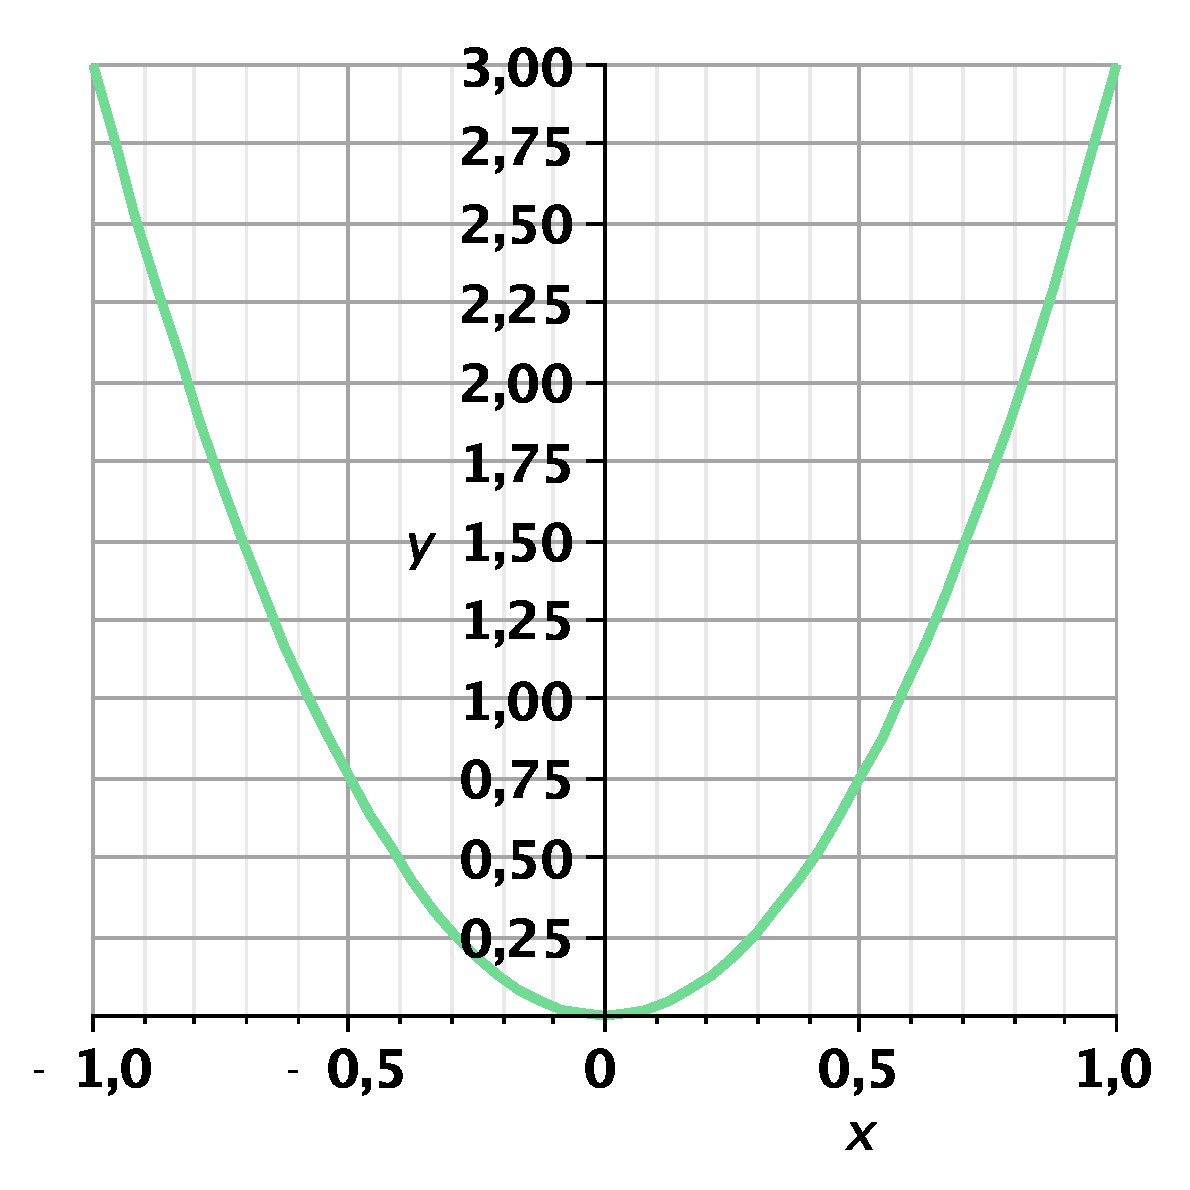
\includegraphics[width=6cm,bb=20 118 575 673]{Q2074v.eps}
 % Q2074v.eps: 1179648x0 pixel, 300dpi, 9987.69x0.00 cm, bb=20 118 575 673
\end{center}
\begin{center}
 \begin{tabular}{|c||c| c | c | c | c |} \hline
{\bf Abscisse ($x$)} & $-1$ & $-0,5$ & 0 & 0,5 & 1 \\ \hline
{\bf Ordonn\'ee ($y$)} & 3 & A & 0 & B & 3 \\ \hline
\end{tabular}
\end{center}
a$)$ A = 0,4 et B = 0,4.\\
b$)$ A = 0,5 et B = 0,5.\\
c$)$ A = 0,75 et B = 0,75.\\
d$)$ A = 1 et B = 1.\\

R\'eponse : c$)$\\

R\'etroaction :\\
\begin{center}
 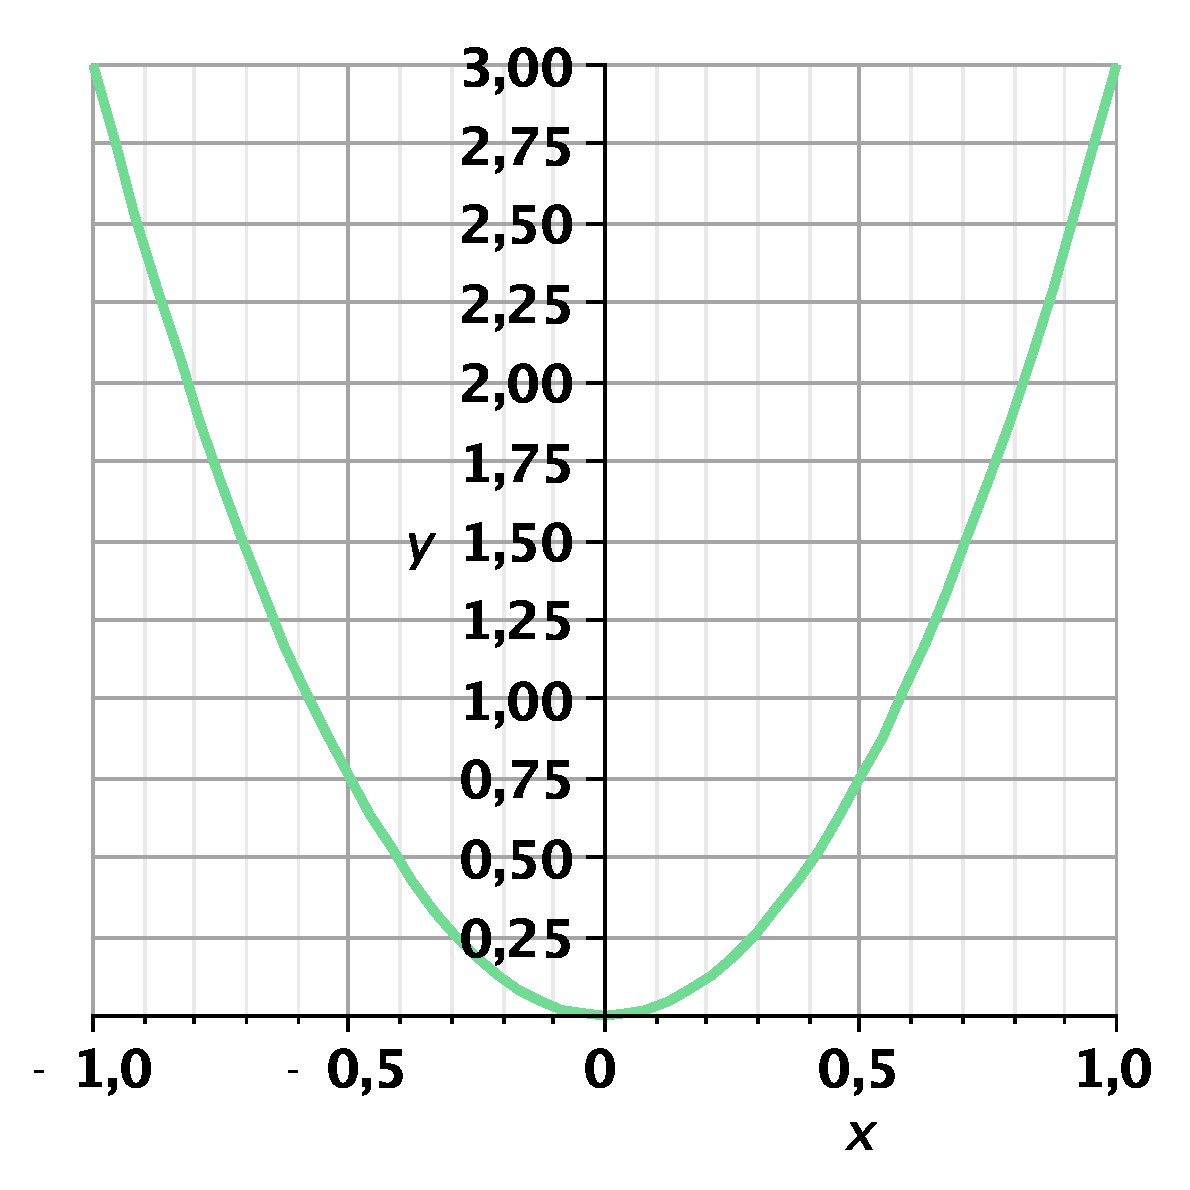
\includegraphics[width=6cm,bb=20 118 575 673]{Q2074v.eps}
 % Q2074v.eps: 1179666x1179666 pixel, 300dpi, 9987.84x9987.84 cm, bb=20 118 575 673
\end{center}
En suivant la courbe du graphique, on peut voir que la valeur de $y$, quand $x$ vaut $-0,5$ et $0,5$, est de $0,75$.\\
Par cons\'equent, la r\'eponse est c$)$.\\

2075-- Voici la table de valeurs repr\'esentant le niveau d'eau dans un bain selon le temps.
\begin{center}
 \begin{tabular}{|c||c| c | c |} \hline
{\bf Temps de remplissage (min)} & 0 & 10 & 20 \\ \hline
{\bf Niveau de l'eau (cm) } & 0 & 15 & 30  \\ \hline
\end{tabular}
\end{center}
Quel graphique repr\'esente correctement cette situation?\\

\begin{tabular}{l l}
 a$)$ & b$)$ \\

 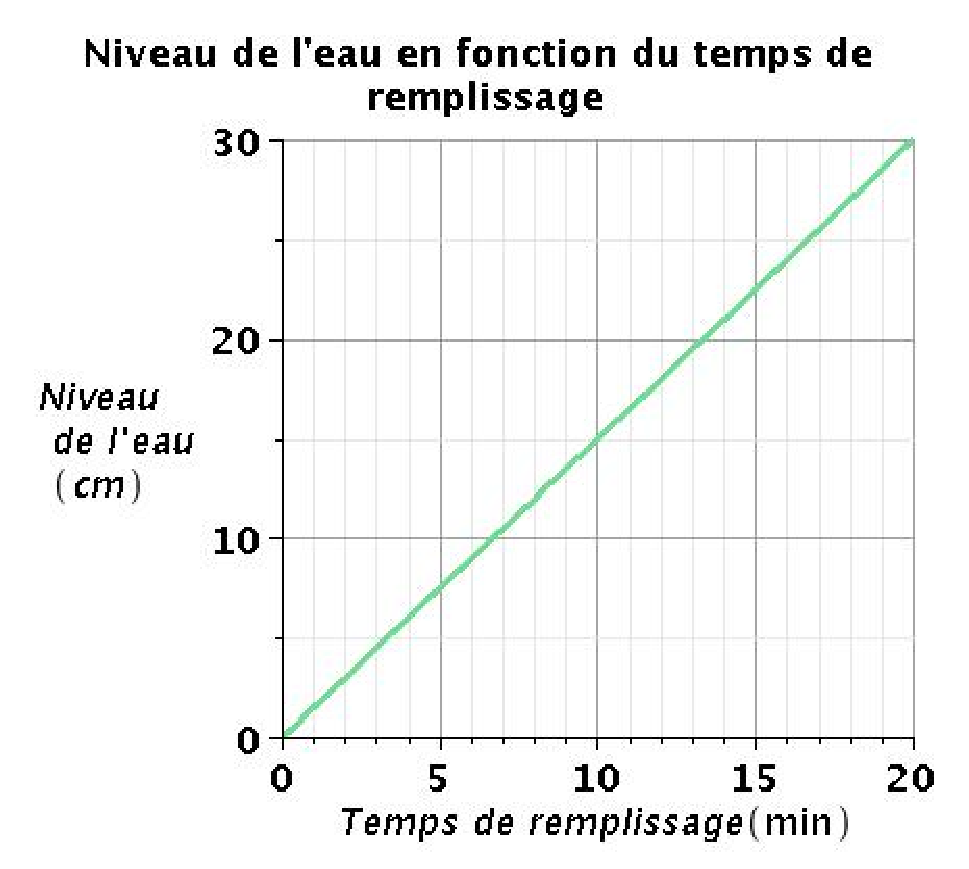
\includegraphics[width=8cm,bb=14 14 463 415]{Q2075b.eps}
 % Q2075b.eps: 1179666x1179666 pixel, 300dpi, 9987.84x9987.84 cm, bb=14 14 463 415


&

 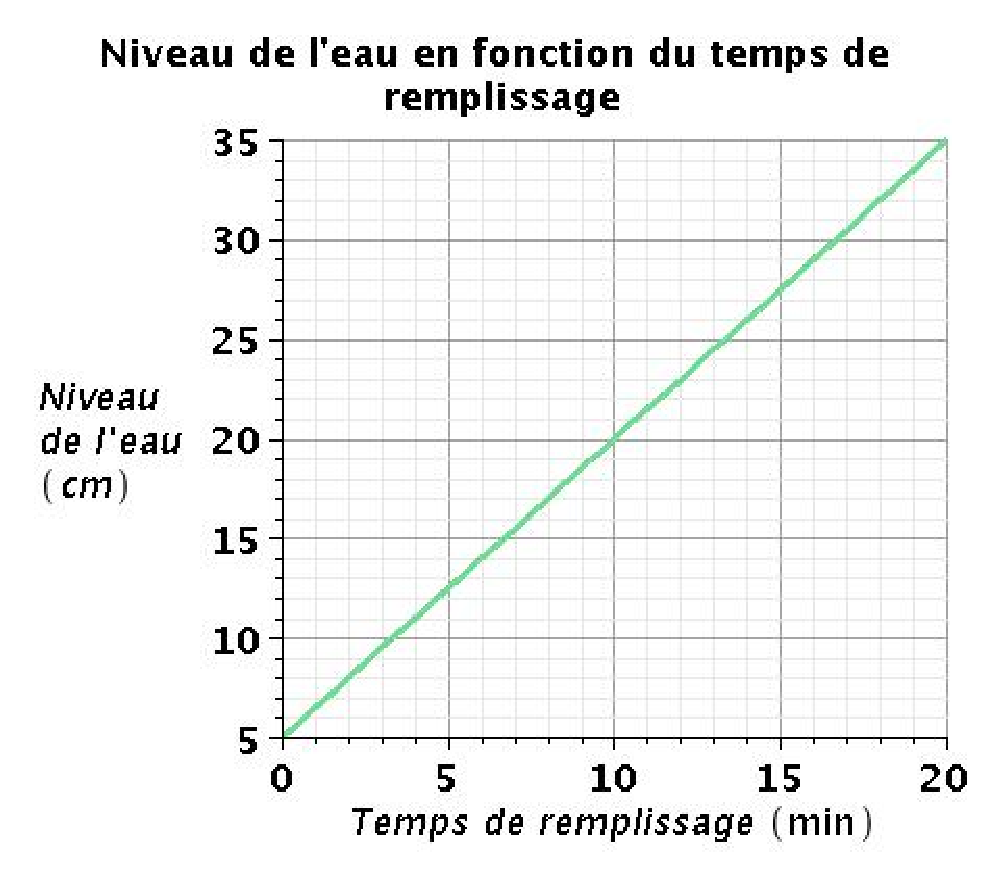
\includegraphics[width=8cm,bb=14 14 479 415]{Q2075c.eps}
 % Q2075c.eps: 1179666x1179666 pixel, 300dpi, 9987.84x9987.84 cm, bb=14 14 479 415

\\
c$)$ & d$)$ \\
 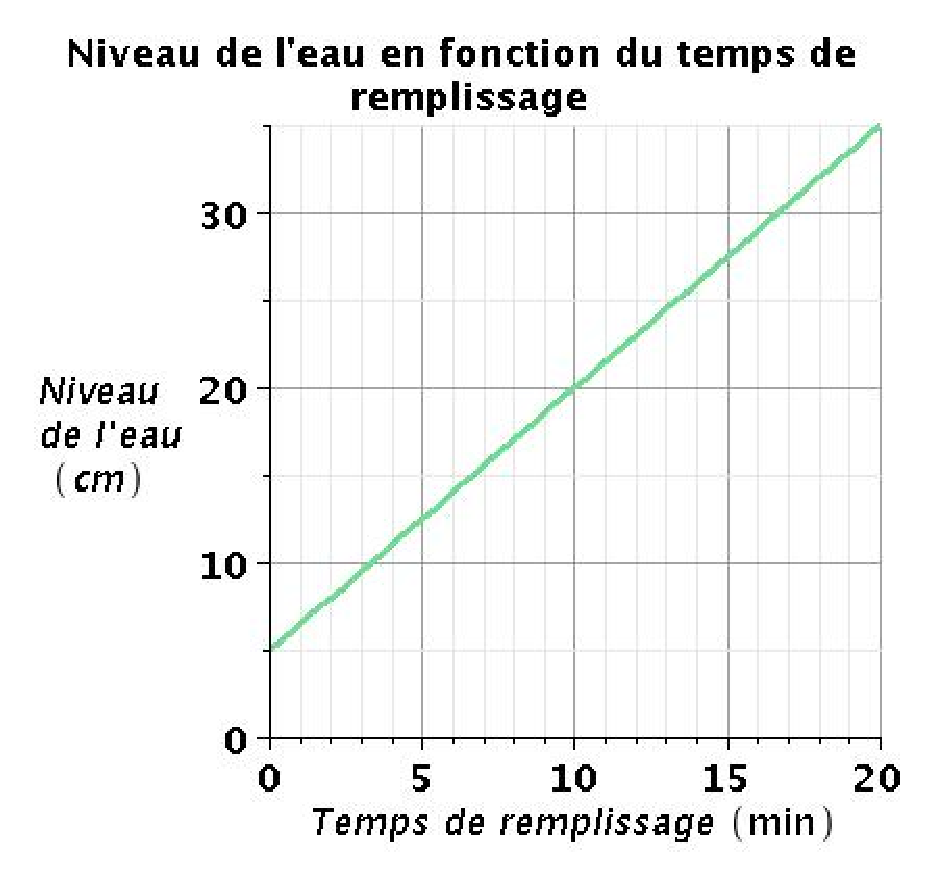
\includegraphics[width=8cm,bb=14 14 447 415]{Q2075d.eps}
 % Q2075d.eps: 1179666x1179666 pixel, 300dpi, 9987.84x9987.84 cm, bb=14 14 447 415

&

 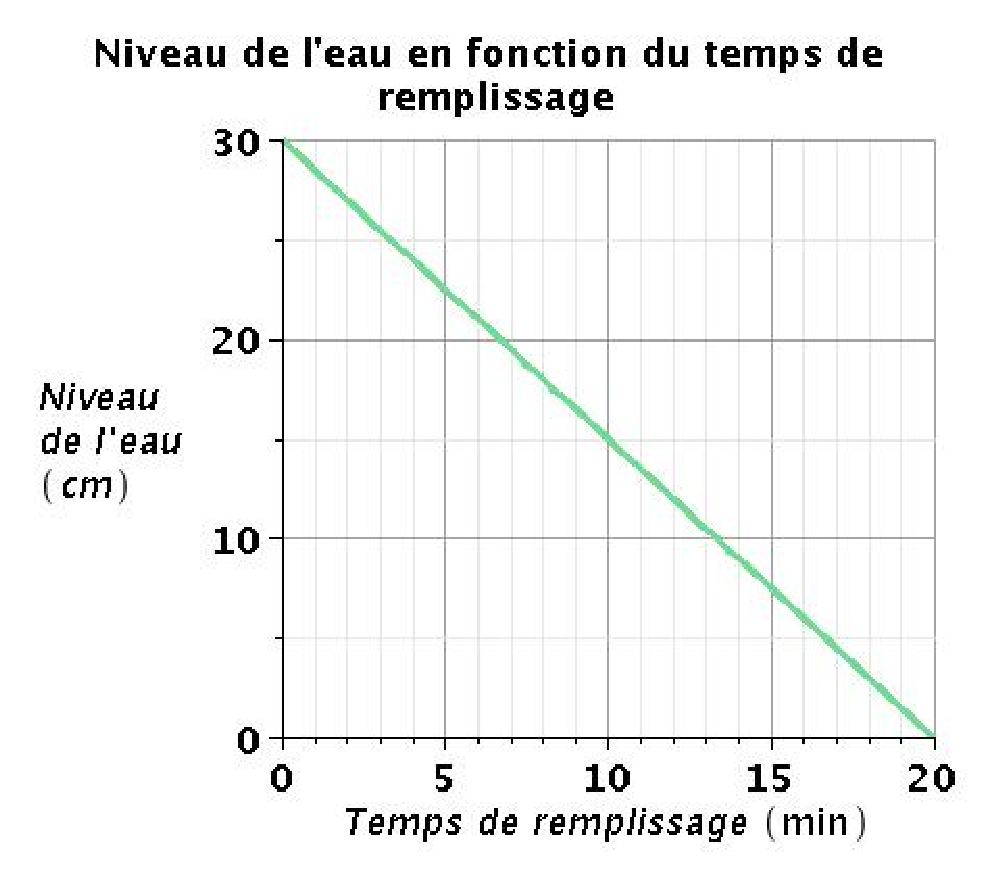
\includegraphics[width=8cm,bb=14 14 473 415]{Q2075e.eps}
 % Q2075e.eps: 1179666x1179666 pixel, 300dpi, 9987.84x9987.84 cm, bb=14 14 473 415

\end{tabular}

R\'eponse : a$)$\\

R\'etroaction :\\
\begin{center}
 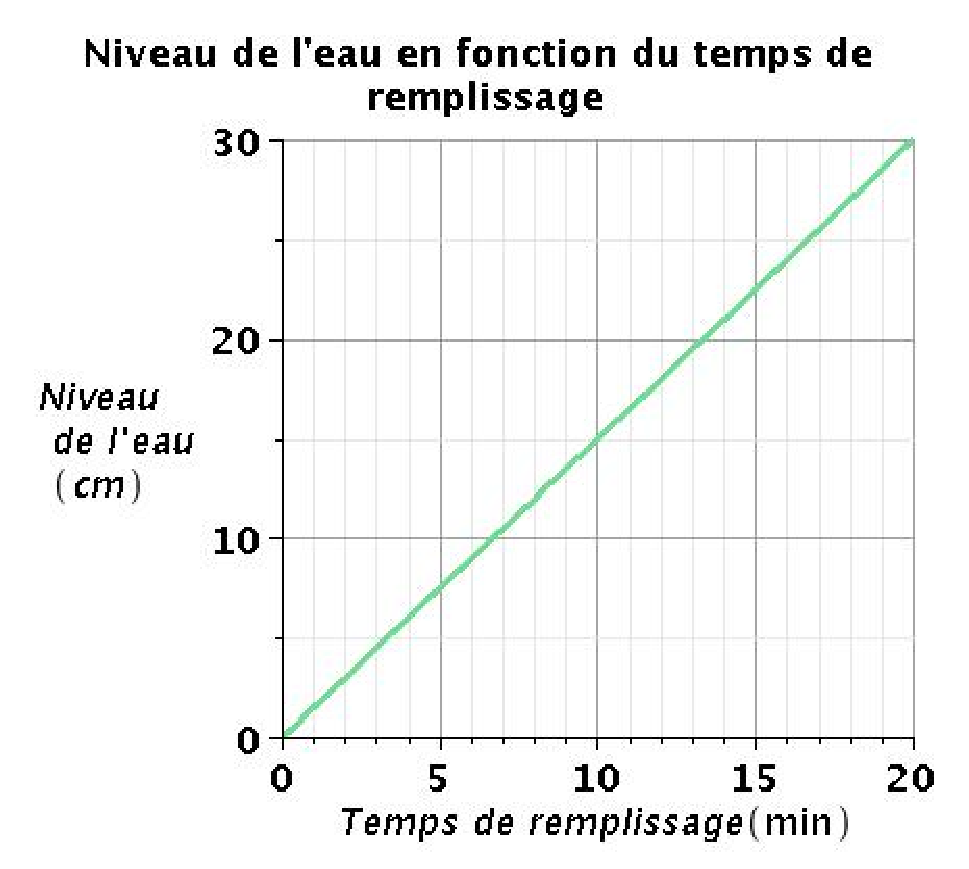
\includegraphics[width=6cm,bb=14 14 463 415]{Q2075b.eps}
 % Q2075b.eps: 1179666x1179666 pixel, 300dpi, 9987.84x9987.84 cm, bb=14 14 463 415
\end{center}
Le graphique qui repr\'esente bien la situation est le graphique a). On peut voir une ordonn\'ee \`a l'origine de 0 et un taux de variation constant et positif.\\
Par cons\'equent, la r\'eponse est a).\\

2076-- Voici la fonction repr\'esentant la vitesse d'une voiture selon le temps.
\begin{equation*}
 y=3x ^ {2}
\end{equation*}
Quel graphique repr\'esente cette situation?

\begin{tabular}{l l}
 a$)$ & b$)$ \\

 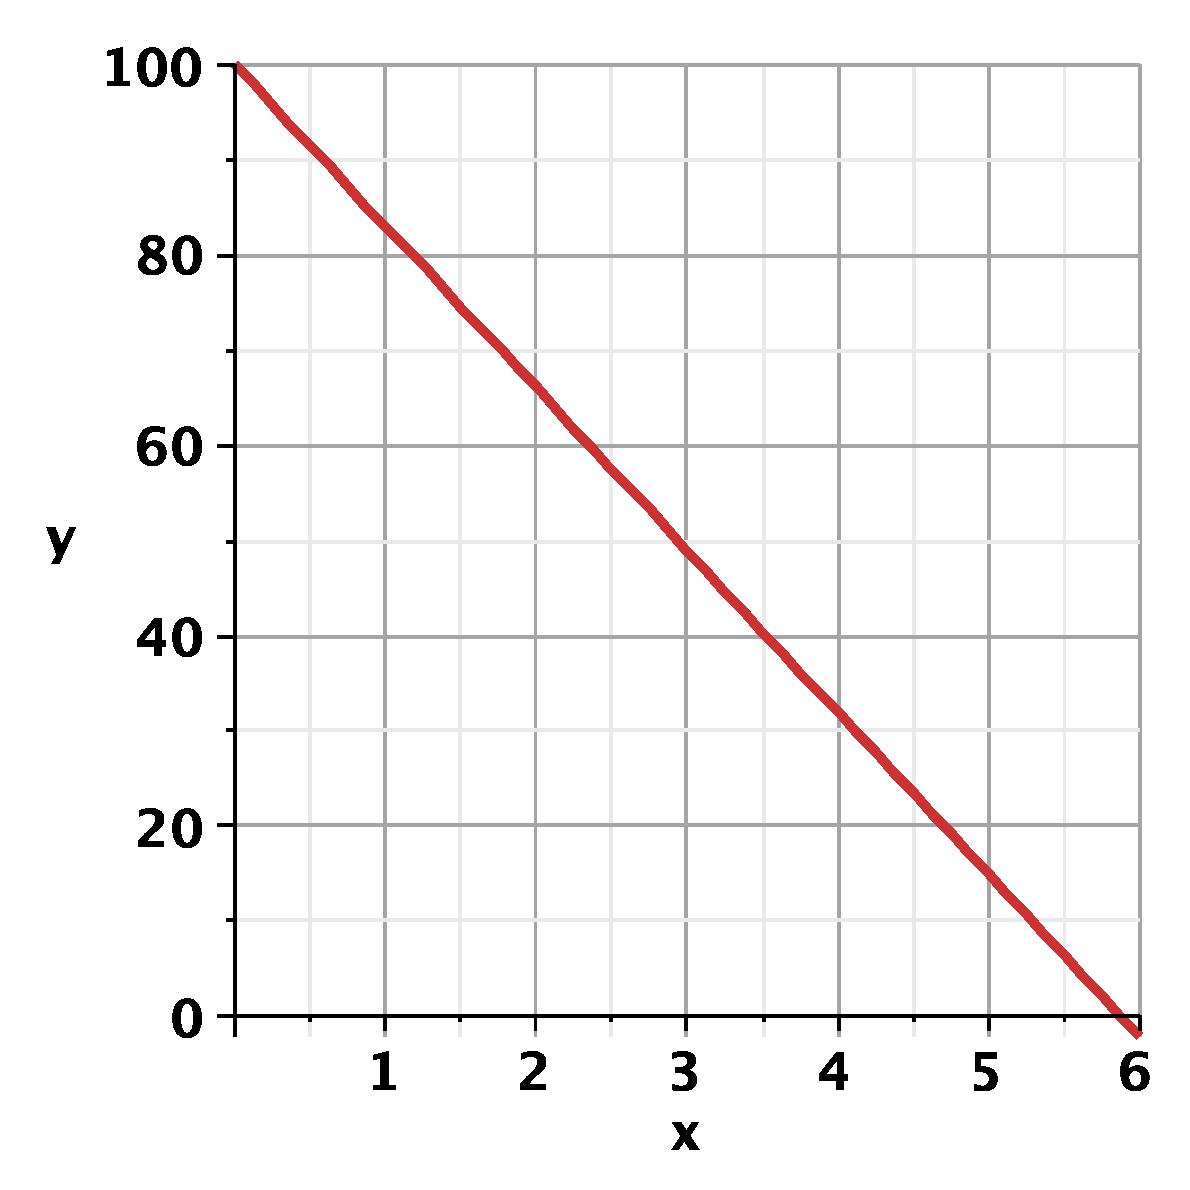
\includegraphics[width=6cm,height=6cm,bb=20 118 575 673]{Q2076a.eps}
 % Q2076a.eps: 1179666x1179666 pixel, 300dpi, 9987.84x9987.84 cm, bb=20 118 575 673

&

 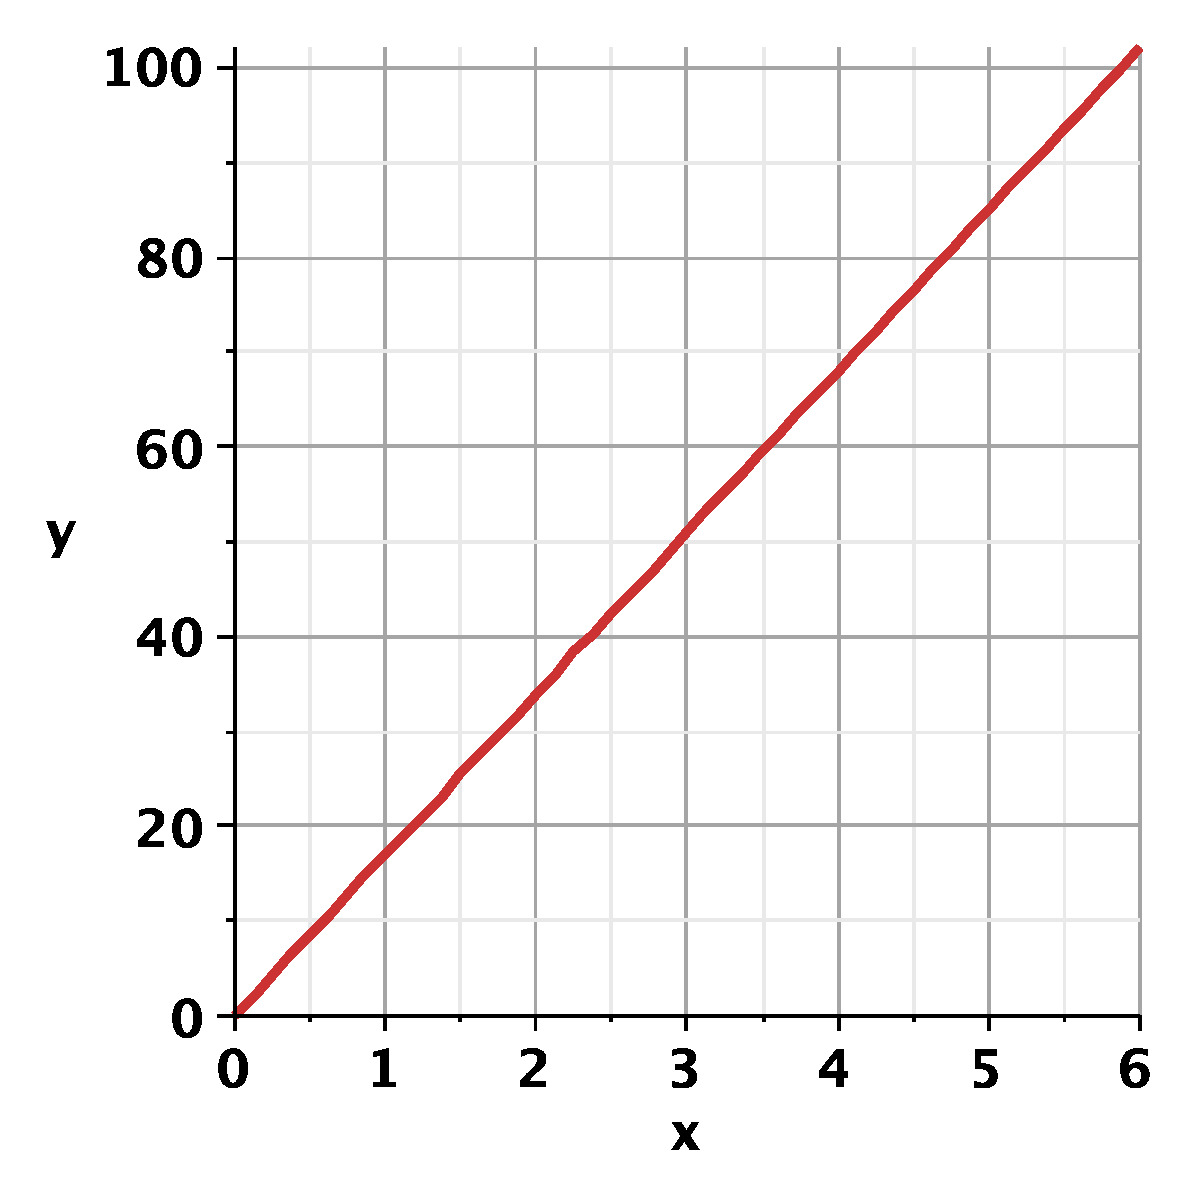
\includegraphics[width=6cm,height=6cm,bb=20 118 575 673]{Q2076b.eps}
 % Q2076b.eps: 1179666x1179666 pixel, 300dpi, 9987.84x9987.84 cm, bb=20 118 575 673
\\
c$)$ & d$)$ \\

 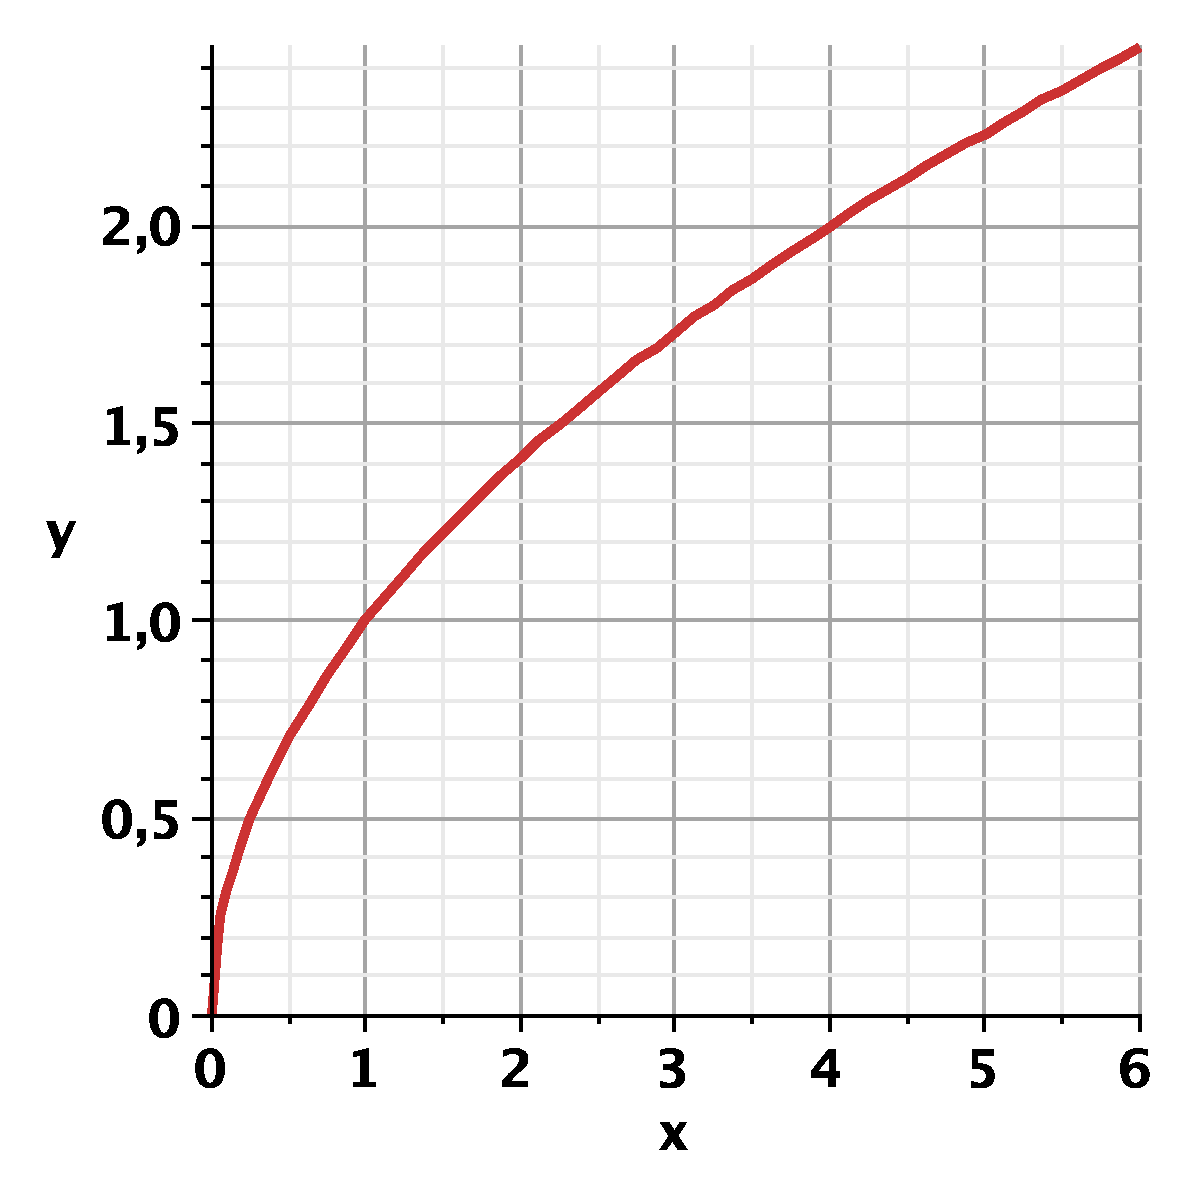
\includegraphics[width=6cm,bb=20 118 575 673]{Q2076cv.eps}
 % Q2076cv.eps: 1179666x1179666 pixel, 300dpi, 9987.84x9987.84 cm, bb=20 118 575 673

&

 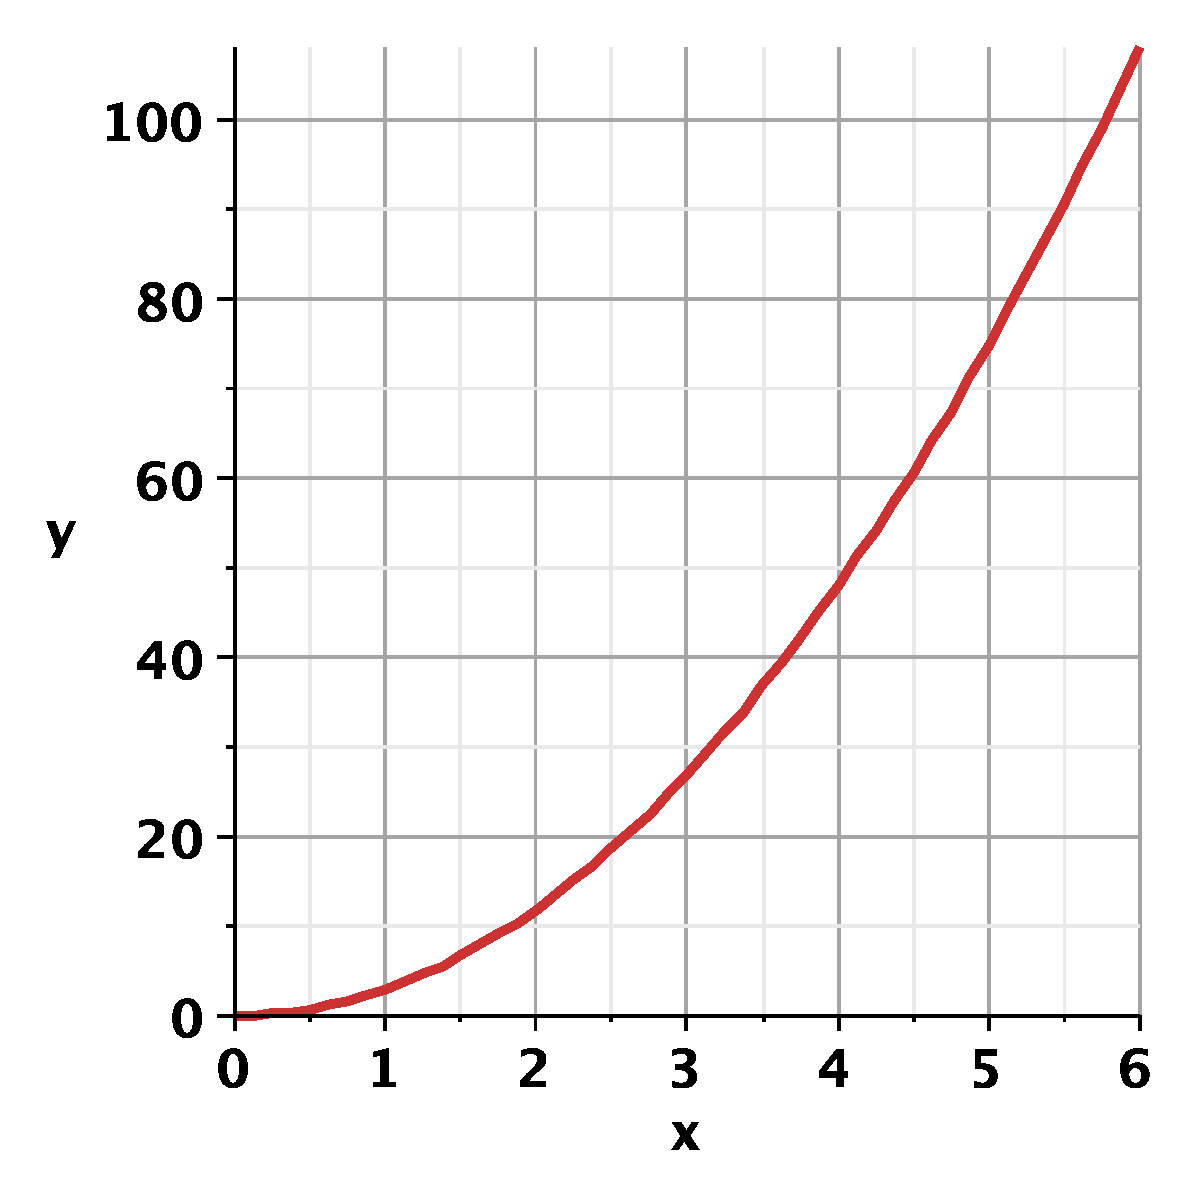
\includegraphics[width=6cm,height=6cm,bb=20 118 575 673]{Q2076d.eps}
 % Q2076d.eps: 1179666x1179666 pixel, 300dpi, 9987.84x9987.84 cm, bb=20 118 575 673


\end{tabular}

R\'eponse : d$)$\\

R\'etroaction :\\
\begin{center}
 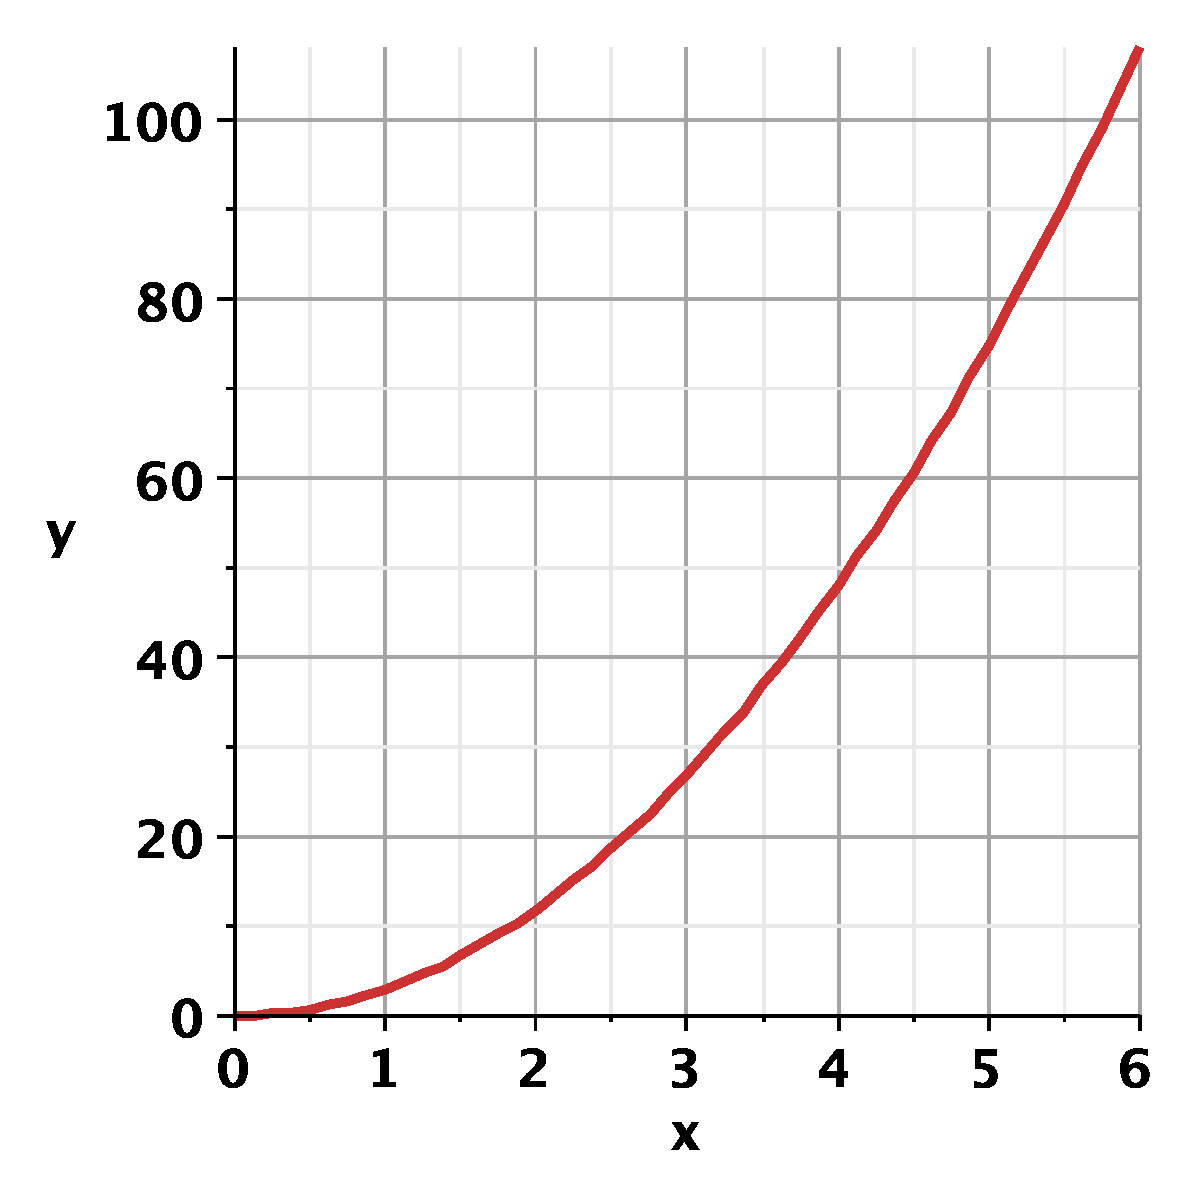
\includegraphics[width=6cm,height=6cm,bb=20 118 575 673]{Q2076d.eps}
 % Q2076d.eps: 1179666x1179666 pixel, 300dpi, 9987.84x9987.84 cm, bb=20 118 575 673
\end{center}
Le graphique qui repr\'esente bien la situation $y=3x^{2}$ est le quatri\`eme graphique. On peut voir une ordonn\'ee \`a l'origine de 0 et une courbe qui repr\'esente bien une fonction du second degr\'e.\\
Par cons\'equent, la r\'eponse est d).\\

2077-- Pour se rendre \`a un spectacle de musique, un groupe de quatre jeunes accompagn\'es par leur enseignant de musique d\'ecident de louer un autobus. Le co\^ut de la location est de 200\$ pour la journ\'ee et l'autobus peut transporter jusqu'\`a 50 personnes. Combien de personnes doivent-ils trouver pour que le transport leur co\^ute 10\$ ou moins?
\begin{center}
 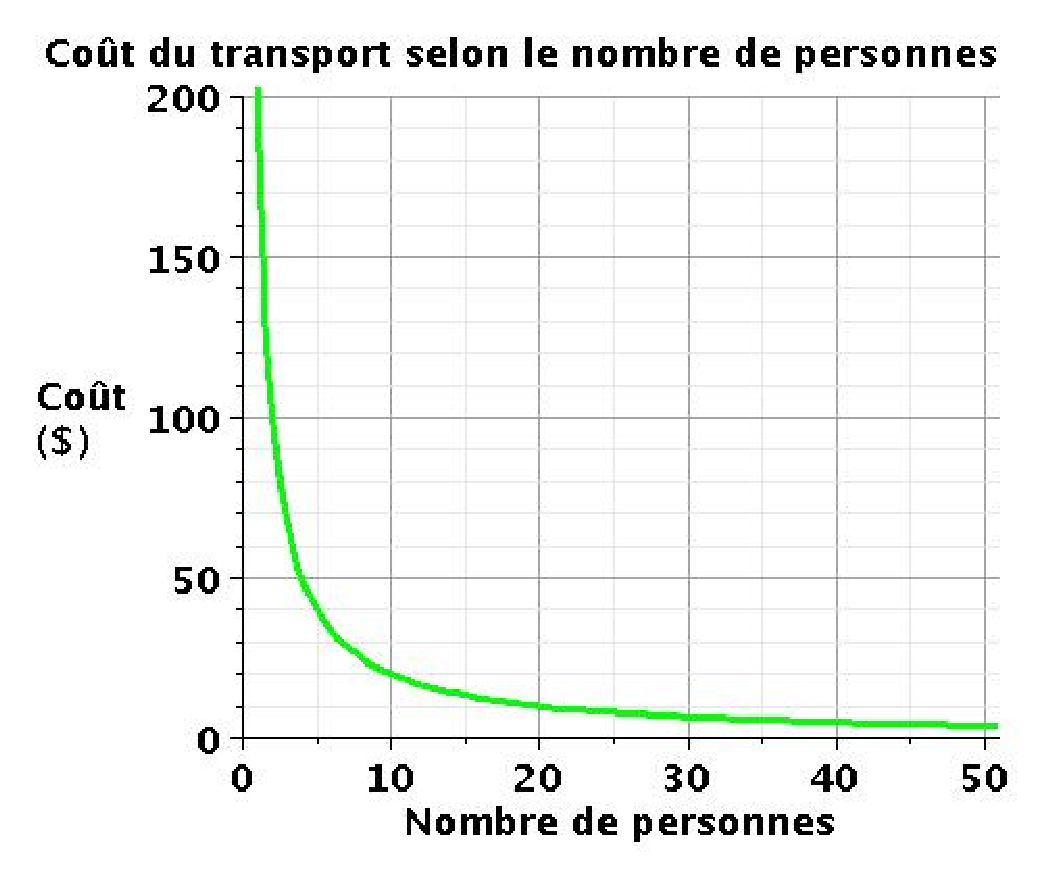
\includegraphics[width=8cm,bb=14 14 497 415]{Q2077.eps}
 % Q2077.eps: 1179666x1179666 pixel, 300dpi, 9987.84x9987.84 cm, bb=14 14 497 415
\end{center}
a$)$ 15\\
b$)$ 16\\
c$)$ 19\\
d$)$ 20\\

R\'eponse : a$)$\\

R\'etroaction :
\begin{center}
 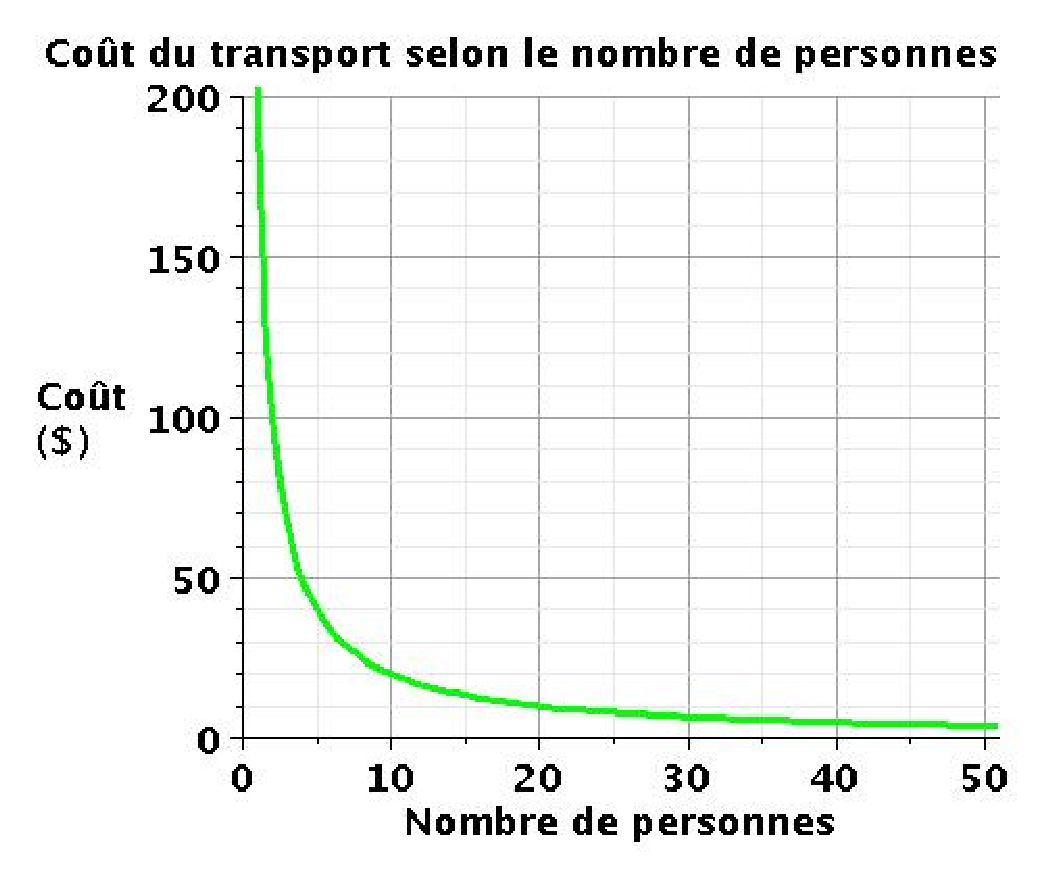
\includegraphics[width=8cm,bb=14 14 497 415]{Q2077.eps}
 % Q2077.eps: 1179666x1179666 pixel, 300dpi, 9987.84x9987.84 cm, bb=14 14 497 415
\end{center}
Dans le graphique, on a le point (20, 10). Donc, pour que le co\^ut soit de 10\$, il doit y avoir \mbox{20 personnes} dans l'autobus. Comme il y a d\'ej\`a les quatre jeunes et l'enseignant qui vont au spectacle, il reste 15 autres personnes \`a trouver. \\
Par cons\'equent, la r\'eponse est a).\\

2078-- Les Lachance veulent faire garder leurs deux enfants le vendredi soir. Ils pr\'evoient \^etre partis six heures. Il peuvent contacter Laura qui demande 5\$ de base plus 2\$ de l'heure ou Michael qui demande 3\$ de l'heure. Qui devraient-ils appeler pour que leur soir\'ee leur co\^ute le moins cher et quel sera le montant \`a payer?\\

a$)$ Ils devraient appeler Laura et cela leur co\^utera 12\$. \\
b$)$ Ils devraient appeler Laura et cela leur co\^utera 17\$. \\
c$)$ Ils devraient appeler Michael et cela leur co\^utera 15\$. \\
d$)$ Ils devraient appeler Michael et cela leur co\^utera 18\$. \\

R\'eponse : b$)$\\

R\'etroaction :\\
\begin{center}
 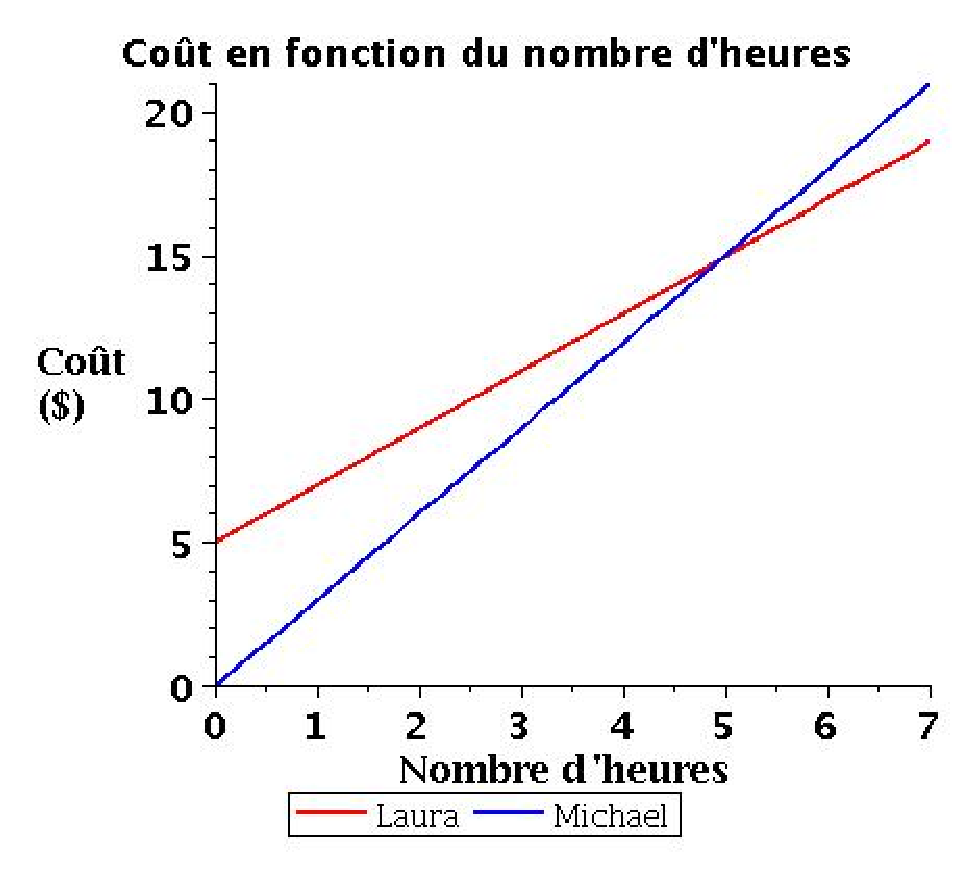
\includegraphics[width=8cm,bb=14 14 465 415]{Q2078.eps}
 % Q2078.eps: 1179666x1179666 pixel, 300dpi, 9987.84x9987.84 cm, bb=14 14 465 415
\end{center}
Pour garder les enfants, Laura demande 5\$ de base plus 2\$ de l'heure.
\begin{eqnarray*}
 5+2\times \textrm{nombre d'heures}
\end{eqnarray*}
Pour travailler six heures, elle demande donc 17\$.
\begin{eqnarray*}
 5+2\times 6 = 17
\end{eqnarray*}
Michael demande 3\$ de l'heure.
\begin{eqnarray*}
 3\times \textrm{nombre d'heures }
\end{eqnarray*}
Pour travailler six heures, il demande donc 18\$.
\begin{eqnarray*}
 3\times 6 = 18
\end{eqnarray*}
Il co\^ute moins cher aux Lachance d'appeler Laura.\\
Par cons\'equent, la r\'eponse est b).\\

2079-- Voici une table de valeurs repr\'esentant un syst\`eme de relations lin\'eaires. D\'etermine la valeur de $y$ de la solution de ce syst\`eme.
\begin{center}
 \begin{tabular}{|c||c| c | c | c | c | c | c | c |} \hline
{\bf $x$} & 0 & 1 & 2 & 3 & 4 & 5 & 6 & 7 \\ \hline
{\bf $y_{1}$} & 3 & 6 & 9 & 12 & 15 & 18 & 21 & 24 \\ \hline
{\bf $y_{2}$} & 5 & 7 & 9 & 11 & 13 & 15 & 17 & 19 \\ \hline
\end{tabular} \\[2mm]
\end{center}

R\'eponse : 9\\

R\'etroaction :\\
\begin{center}
 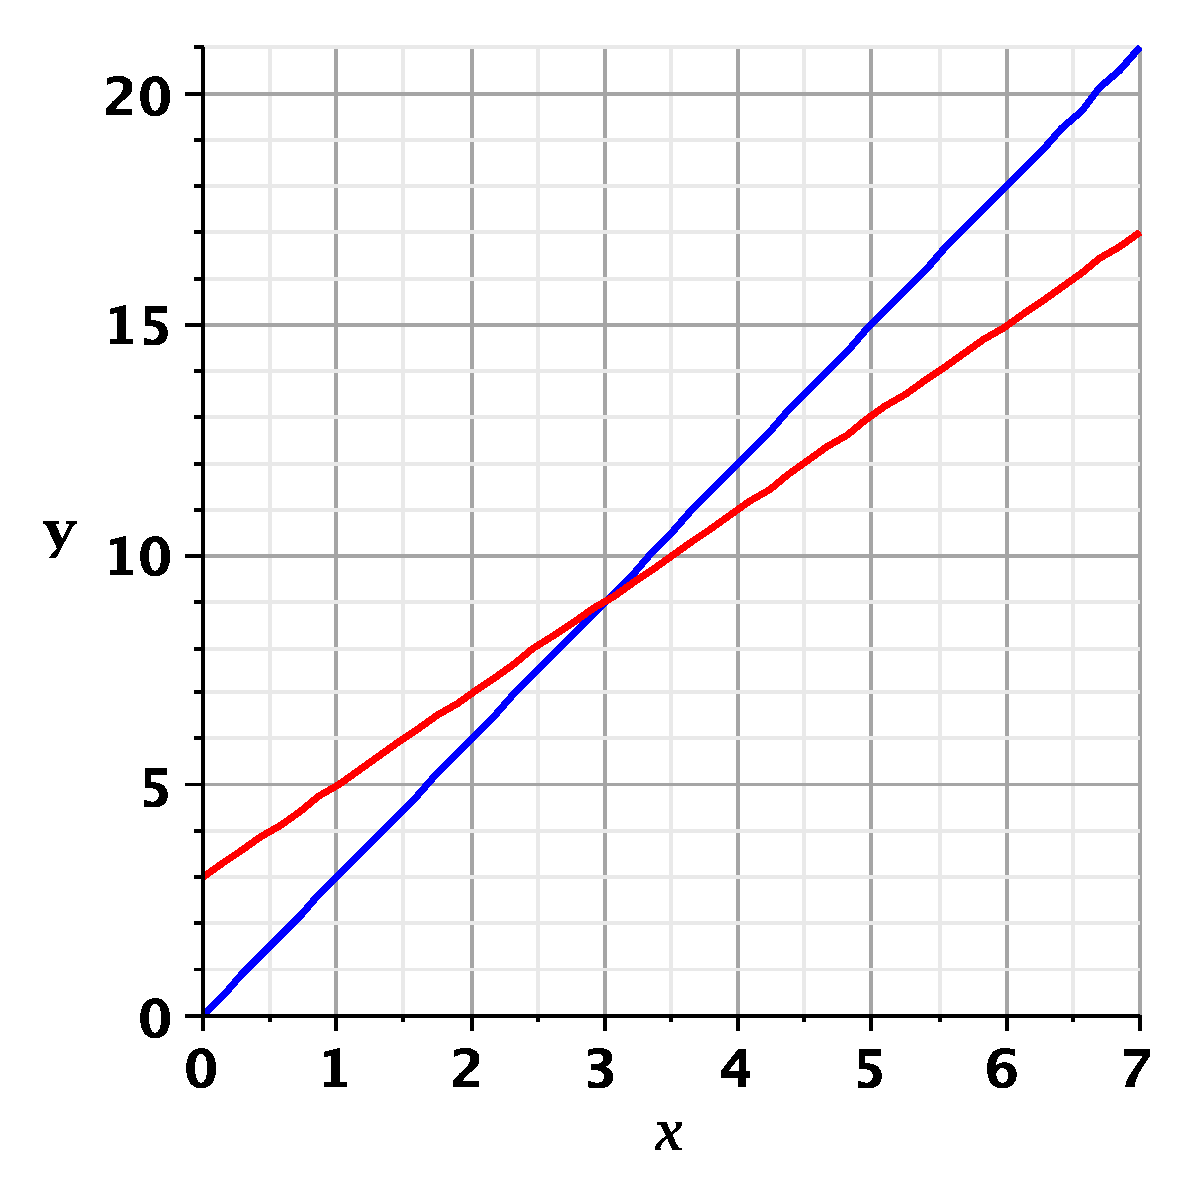
\includegraphics[width=6cm,bb=20 118 575 673]{Q2079.eps}
 % Q2079.eps: 1179666x1179666 pixel, 300dpi, 9987.84x9987.84 cm, bb=20 118 575 673
\end{center}
Pour r\'esoudre un syst\`eme, il faut trouver la valeur de la variable ind\'ependante pour laquelle les variables d\'ependantes prennent la m\^eme valeur. Dans la table de valeurs, on remarque que pour la valeur $x$ = 2, les variables d\'ependantes prennent la m\^eme valeur, soit 9.\\
Par cons\'equent, la r\'eponse est 9.\\

%Questions sur les fonctions mathematiques 416 difficulte 3

2080-- Alexandre ramasse de l'argent pour s'acheter un v\'elo de 450\$. Il distribue des journaux dans son quartier et a accumul\'e 230\$. Il peut mettre de c\^ot\'e 30\$ par semaine. Il se fait une table de valeurs pour savoir quand il pourra faire son achat. \\
Aide Alexandre \`a trouver les variables d\'ependante et ind\'ependante de cette situation.\\

\begin{tabular}{l l l}
a$)$ & Variable d\'ependante: argent accumul\'e & Variable ind\'ependante: nombre de semaines\\
b$)$ & Variable d\'ependante: argent accumul\'e & Variable ind\'ependante: co\^ut du v\'elo\\
c$)$ & Variable d\'ependante: co\^ut du v\'elo & Variable ind\'ependante: argent accumul\'e\\
d$)$ & Variable d\'ependante: nombre de semaines & Variable ind\'ependante: co\^ut du v\'elo\\
\end{tabular}\\[2mm]
\\
R\'eponse : a$)$ \\

R\'etroaction :\\
La variable d\'ependante de cette situation est l'argent accumul\'e et la variable ind\'ependante est le nombre de semaines. En effet, on a bien que le montant d'argent accumul\'e d\'epend du nombre de semaines qu'il a travaill\'e.\\
Par cons\'equent, la r\'eponse est a).\\ \\

2081-- Voici la table de valeurs d'une fonction de variation partielle dont l'\'equation est $y = 2x + 2$.
\begin{center}
 \begin{tabular}{|c|c|} \hline
{\bf Abscisse ($x$)} & {\bf Ordonn\'ee ($y$)}  \\ \hline \hline
3 & 8 \\ \hline
4 & 10 \\ \hline
5 & 12 \\ \hline
6 & 14 \\ \hline
7 & 16 \\ \hline
$\ldots$ & $\ldots$ \\ \hline
\multicolumn{2}{c}{}\\
\end{tabular}
\end{center}
Quelle est la valeur initiale?\\

R\'eponse : 2\\

R\'etroaction :\\
\begin{center}
 \includegraphics[width=6cm,bb=20 118 575 673]{Q2081.eps}
 % Q2081.eps: 1179666x1179666 pixel, 300dpi, 9987.84x9987.84 cm, bb=20 118 575 673
\end{center}
Dans une fonction de variation partielle, la valeur initiale, toujours diff\'erente de 0, est la valeur de la variable d\'ependante lorsque la variable ind\'ependante vaut 0. Il faut donc calculer ce que vaut $y$ lorsque $x=0$.
\begin{eqnarray*}
 y &=& 2x + 2 \\
 y &=& (2 \times 0) + 2 \\
 y &=& 2
\end{eqnarray*}
Par cons\'equent, la r\'eponse est 2.\\

2082-- Les employ\'es de la ville doivent vider la piscine municipale pour l'hiver. Voici le graphique repr\'esentant la quantit\'e d'eau dans la piscine selon le temps. Quel est le d\'ebit (en litres par heure) d'\'ecoulement de l'eau?\\
\begin{center}
 \includegraphics[width=8cm,bb=14 14 529 415]{Q2082v.eps}
 % Q2082v.eps: 1179666x1179666 pixel, 300dpi, 9987.84x9987.84 cm, bb=14 14 529 415
\end{center}

a$)$ $\frac{-1}{4 000}$\\[2mm]
b$)$ $-4 000$\\ [2mm]
c$)$ $\frac{1}{4 000}$\\[2mm]
d$)$ 4 000\\

R\'eponse : b$)$\\

R\'etroaction :\\
\begin{center}
 \includegraphics[width=8cm,bb=14 14 529 415]{Q2082v.eps}
 % Q2082v.eps: 1179666x1179666 pixel, 300dpi, 9987.84x9987.84 cm, bb=14 14 529 415
\end{center}
Pour conna\^itre le d\'ebit auquel la piscine se vide, il suffit de calculer la pente de la fonction.\\
\begin{eqnarray*}
\textrm{d\'ebit} &=& \frac{\textrm{variation en $y$}}{\textrm{variation en $x$}} \\ [2mm]
&=& \frac{80 000-0}{0-20}\\ [2mm]
&=& \frac{-80 000}{20}\\ [2mm]
&=& -4 000\\ [2mm]
\end{eqnarray*}
Par cons\'equent, la r\'eponse est b).\\

2083-- Jonathan veut s'acheter un ordinateur portable. Il \'economise depuis un bon moment et il a accumul\'e 600\$. L'ordinateur qu'il d\'esire co\^ute 850\$ et il peut mettre 30\$ de c\^ot\'e par semaine. Il se demande dans combien de semaines il pourra acheter l'ordinateur.\\
Quel type de fonction repr\'esente le mieux la situation?\\

a$)$ Une fonction de variation directe\\
b$)$ Une fonction de variation inverse\\
c$)$ Une fonction de variation partielle\\
d$)$ Une fonction du second degr\'e\\

R\'eponse : c$)$\\

R\'etroaction :\\
La situation est le mieux repr\'esent\'ee par une relation de variation partielle. Son ordonn\'ee \`a l'origine est 600 et son taux de variation est 30. On obtient donc la formule $y=30x + 600$.\\
Par cons\'equent, la r\'eponse est c).\\

2084-- Guillaume veut s'acheter un ordinateur portable. Il \'economise depuis un bon moment et il a accumul\'e 400\$. L'ordinateur qu'il d\'esire co\^ute 850\$ et il peut mettre 40\$ de c\^ot\'e par semaine. Dans combien de semaines pourra-t-il acheter l'ordinateur?\\

R\'eponse : 12\\

R\'etroaction :\\
Pour trouver dans combien de semaines il pourra acheter l'ordinateur, il faut trouver l'\'equation de la fonction associ\'ee \`a la situation. Il a d\'ej\`a accumul\'e 400\$ et il peut mettre 40\$ de c\^ot\'e par semaine. L'ordonn\'ee \`a l'origine est donc 400 et le taux de variation est 40.\\
On a donc la formule $y=40x + 400$.
\begin{center}
 \includegraphics[width=6cm,bb=14 14 481 415]{Q2084v.eps}
 % Q2084v.eps: 1179666x1179666 pixel, 300dpi, 9987.84x9987.84 cm, bb=14 14 481 415
\end{center}
On cherche la valeur de $x$ quand $y=850$.
\begin{eqnarray*}
 y&=&40x + 400\\
850&=&40x + 400\\
850-400&=&40x + 400-400\\
450&=&40x\\[2mm]
\frac{450}{40}&=&\frac{40x}{40}\\[2mm]
11,25&=&x
\end{eqnarray*}
Comme 11,25 n'est pas un entier, on arrondit la r\'eponse \`a l'entier sup\'erieur, soit 12. On a donc que, dans 12 semaines, il pourra acheter l'ordinateur.\\
Par cons\'equent, la r\'eponse est 12.\\

2085-- Une cellule vivante se divise en deux autres cellules vivantes \`a chaque minute. Le processus peut continuer ind\'efiniment. Combien de cellules a-t-on apr\`es dix minutes?\\

a$)$ $\frac{2}{(10\times2)}$\\[2mm]
b$)$ $\frac{2}{10}$\\[2mm]
c$)$ $2 \times 10$\\[2mm]
d$)$ $2^{10}$\\

R\'eponse : d$)$\\

R\'etroaction :\\
\`A la premi\`ere minute, on a une cellule qui en devient deux. \`A la deuxi\`eme minute, on a deux cellules qui en deviennent quatre \ldots \\
\begin{eqnarray*}
 1 &\to& 2\\
2 &\to& 4 = 2 \times 2\\
4 &\to& 8 = 2 \times 2  \times 2\\
8 &\to& 16 = 2 \times 2  \times 2 \times 2\\
\ldots &\to& \ldots
\end{eqnarray*}

Voici la table de valeurs correspondant \`a la situation:\\[2mm]
\begin{tabular}{|c||c| c | c | c | c | c | c | c | c | c | c |} \hline
{\bf Nombre de minutes} & 0 & 1 & 2 & 3 & 4 & 5 & 6 & 7 & 8 & 9 & 10\\ \hline
\multirow{2}*{\bf Nombre de cellules} & \multirow{2}*{$2^{0}$} & \multirow{2}*{$2^{1}$} & \multirow{2}*{$2^{2}$} & \multirow{2}*{$2^{3}$} & \multirow{2}*{$2^{4}$} & \multirow{2}*{$2^{5}$} & \multirow{2}*{$2^{6}$} & \multirow{2}*{$2^{7}$} & \multirow{2}*{$2^{8}$} & \multirow{2}*{$2^{9}$} & \multirow{2}*{$2^{10}$} \\
{ } & \multirow{2}*{} & \multirow{2}*{} & \multirow{2}*{} & \multirow{2}*{} & \multirow{2}*{} & \multirow{2}*{} & \multirow{2}*{} & \multirow{2}*{} & \multirow{2}*{} & \multirow{2}*{} & \multirow{2}*{} \\ \hline
\end{tabular}\\[2mm]

Par cons\'equent, la r\'eponse est d).\\

2086-- Vrai ou faux? La table suivante correspond \`a une relation de variation exponentielle.\\
\begin{center}
 \begin{tabular}{|c||c| c | c | c | c | c | c | c |} \hline
{\bf $x$} & 0 & 1 & 2 & 3 & 4 & 5 & 6 & \ldots \\ \hline
{\bf $y$} & 0 & 2 & 8 & 18 & 32 & 50 & 72 & \ldots \\ \hline
\end{tabular}\\[2mm]
\end{center}

R\'eponse : faux\\

R\'etroaction :\\
La table de valeurs ne correspond pas \`a une relation de variation exponentielle.
\begin{center}
 \begin{tabular}{|c||c| c | c | c | c | c | c | c |} \hline
{\bf $x$} & 0 & 1 & 2 & 3 & 4 & 5 & 6 & \ldots \\ \hline
{\bf $y$} & 0 & 2 & 8 & 18 & 32 & 50 & 72 & \ldots \\ \hline
\end{tabular}\\[2mm]
\end{center}
Si on calcule les taux de variation unitaires, on obtient la suite suivante.
\begin{center}
 2, 6, 10, 14, 18, 22
\end{center}
Cette suite ne correspond pas \`a la suite que l'on obtiendrait si on avait une relation de variation exponentielle. De plus, si on fait le graphique de cette table, on obtient ceci:\\
\begin{center}
 \includegraphics[width=6cm,bb=20 118 575 673]{Q2086.eps}
 % Q2086.eps: 1179666x1179666 pixel, 300dpi, 9987.84x9987.84 cm, bb=20 118 575 673
\end{center}
Ce graphique correspond plut\^ot \`a une fonction du second degr\'e.\\
Par cons\'equent, la r\'eponse est: faux.\\

2087--  Vrai ou faux? La table suivante correspond \`a une relation de variation exponentielle.
\begin{center}
 \begin{tabular}{|c||c| c | c | c | c | c | c |} \hline
{\bf $x$} & 0 & 1 & 2 & 3 & 4 & 5 & \ldots \\ \hline
\multirow{2}*{\bf $y$} & \multirow{2}*{1} & \multirow{2}*{$\frac{1}{5}$} & \multirow{2}*{$\frac{1}{25}$} & \multirow{2}*{$\frac{1}{125}$} & \multirow{2}*{$\frac{1}{625}$} & \multirow{2}*{$\frac{1}{3125}$} & \multirow{2}*{\ldots} \\
\multirow{2}*{} & \multirow{2}*{} & \multirow{2}*{} & \multirow{2}*{} & \multirow{2}*{} & \multirow{2}*{} & \multirow{2}*{} & \multirow{2}*{} \\\hline
\end{tabular}\\[2mm]
\end{center}

R\'eponse : vrai\\

R\'etroaction :\\
La table de valeurs correspond \`a une relation de variation exponentielle.
\begin{center}
 \begin{tabular}{|c||c| c | c | c | c | c | c |} \hline
{\bf $x$} & 0 & 1 & 2 & 3 & 4 & 5 & \ldots \\ \hline
\multirow{2}*{\bf $y$} & \multirow{2}*{1} & \multirow{2}*{$\frac{1}{5}$} & \multirow{2}*{$\frac{1}{25}$} & \multirow{2}*{$\frac{1}{125}$} & \multirow{2}*{$\frac{1}{625}$} & \multirow{2}*{$\frac{1}{3125}$} & \multirow{2}*{\ldots} \\
\multirow{2}*{} & \multirow{2}*{} & \multirow{2}*{} & \multirow{2}*{} & \multirow{2}*{} & \multirow{2}*{} & \multirow{2}*{} & \multirow{2}*{} \\\hline
\end{tabular}\\[2mm]
\end{center}
Si on calcule les taux de variation unitaires, on obtient la suite suivante.
\begin{eqnarray*}
 -\frac{4}{5}, -\frac{4}{25}, -\frac{4}{125}, -\frac{4}{625}, -\frac{4}{3125}
\end{eqnarray*}
Cette suite correspond bien \`a la suite que l'on obtient si on a une relation de variation exponentielle puisqu'elle montre l'existence d'un facteur correspondant \`a la base de la variation exponentielle. De plus, si on fait le graphique de cette table, on obtient ceci:
\begin{center}
 \includegraphics[width=6cm,bb=20 118 575 673]{Q2087v.eps}
 % Q2087v.eps: 1179666x1179666 pixel, 300dpi, 9987.84x9987.84 cm, bb=20 118 575 673
\end{center}
Ce graphique correspond bien \`a une fonction de variation exponentielle.\\
Par cons\'equent, la r\'eponse est: vrai.\\

2088-- Eric et Julie s'entra\^inent r\'eguli\`erement \`a la course. Ils courent en moyenne 10 kilom\`etres \`a chaque entra\^inement. Hier, Eric n'\'etait pas disponible et Julie est partie courir seule. Dix minutes plus tard, Eric d\'ecide de la rejoindre.  Si Julie court \`a une vitesse de 1 kilom\`etre en 5 minutes et Eric 1 kilom\`etre en 4 minutes, est-ce que Eric va r\'eussir \`a rejoindre Julie avant la fin des 10 kilom\`etres?\\

a$)$ Non, Julie va arriver en premier.\\
b$)$ Non, il va rejoindre Julie exactement \`a la fin des 10 kilom\`etres.\\
c$)$ Oui, il va rejoindre Julie bien avant la fin des 10 kilom\`etres.\\
d$)$ Oui, car les gar\c cons courent toujours plus vite que les filles.\\

R\'eponse : b$)$\\

R\'etroaction :\\
\begin{center}
 \includegraphics[width=8cm,bb=20 177 575 614]{Q2088.eps}
 % Q2088.eps: 1179668x1179668 pixel, 300dpi, 9987.86x9987.86 cm, bb=20 177 575 614
\end{center}
Eric rejoindra Julie \`a la toute fin des 10 kilom\`etres. Pour trouver la r\'eponse, il faut trouver les \'equations des deux relations associ\'ees \`a la situation. Tout d'abord, la relation li\'ee \`a Julie est trouv\'ee comme suit:
\begin{itemize}
\item Son taux de variation est $\frac{1}{5}$km/min car elle court \`a une vitesse de 1 kilom\`etre en 5 minutes.
\item Son ordonn\'ee \`a l'origine est 0.
\end{itemize}
On a donc l'\'equation $y=\frac{x}{5}$.\\

Pour la relation li\'ee \`a Eric, on trouve:
\begin{itemize}
\item Son taux de variation est $\frac{1}{4}$km/min car il court \`a une vitesse de 1 kilom\`etre en 4 minutes.
\item Son ordonn\'ee \`a l'origine est $-2,5$. Elle est calcul\'ee comme suit:
\begin{eqnarray*}
y&=&\frac{x}{4}+b\\[2mm]
0&=&\frac{10}{4}+b\\[2mm]
0&=&2,5+b\\[2mm]
-2,5&=&b
\end{eqnarray*}
\end{itemize}
On a donc l'\'equation $y=\frac{x}{4}-2,5$.\\

Pour savoir si Eric retrouve Julie avant la fin du 10 kilom\`etres, on peut remplacer $y$ par 10 dans les deux \'equations et trouver les valeurs de $x$ correspondantes.
\begin{eqnarray*}
y&=&\frac{x}{5}\\[2mm]
10&=&\frac{x}{5}\\[2mm]
50&=&x
\end{eqnarray*}
Pour Julie, on trouve qu'elle a couru 10 kilom\`etres en 50 minutes.
\begin{eqnarray*}
y&=&\frac{x}{4}-2,5\\[2mm]
10&=&\frac{x}{4}-2,5\\[2mm]
10+2,5&=&\frac{x}{4}-2,5+2,5\\[2mm]
12,5&=&\frac{x}{4}\\[2mm]
4\times 12,5&=&4\times \frac{x}{4}\\[2mm]
50&=&x
\end{eqnarray*}
Pour Eric, on trouve qu'il est arriv\'e \`a la fin des 10 kilom\`etres 50 minutes apr\`es le d\'epart de Julie. Donc, il l'a rejoint seulement \`a la fin des 10 kilom\`etres.\\
Par cons\'equent, la r\'eponse est b).\\

2089-- Eric et Julie s'entra\^inent r\'eguli\`erement \`a la course. Ils courent en moyenne 5 kilom\`etres \`a chaque entra\^inement. Hier, Eric n'\'etait pas disponible et Julie est partie courir seule. Eric d\'ecide de la rejoindre sept minutes plus tard.  Si Julie court \`a une vitesse de 1 kilom\`etre en 5 minutes et Eric 1 kilom\`etre en 4 minutes, est-ce qu'Eric va r\'eussir \`a rejoindre Julie avant la fin des 5 kilom\`etres?\\

a$)$ Non, Julie va arriver en premier.\\
b$)$ Non, il va rejoindre Julie exactement \`a la fin des 5 kilom\`etres.\\
c$)$ Oui, il va rejoindre Julie bien avant la fin des 5 kilom\`etres.\\
d$)$ Oui, car les gar\c cons courent toujours plus vite que les filles.\\

R\'eponse : a$)$\\

R\'etroaction :\\
\begin{center}
 \includegraphics[width=8cm,bb=20 172 575 619]{Q2089.eps}
 % Q2089.eps: 1179648x0 pixel, 300dpi, 9987.69x0.00 cm, bb=20 172 575 619
\end{center}
Julie arrivera avant Eric. Pour trouver la r\'eponse, il faut trouver les \'equations des deux relations associ\'ees \`a la situation. Tout d'abord, la relation li\'ee \`a Julie est trouv\'ee comme suit:
\begin{itemize}
\item Son taux de variation est $\frac{1}{5}$km/min car elle court \`a une vitesse de 1 kilom\`etre en 5 minutes.
\item Son ordonn\'ee \`a l'origine est 0.
\end{itemize}
On a donc l'\'equation $y=\frac{x}{5}$.\\

Pour la relation li\'ee \`a Eric, on trouve:
\begin{itemize}
\item Son taux de variation est $\frac{1}{4}$km/min car il court \`a une vitesse de 1 kilom\`etre en 4 minutes.
\item Son ordonn\'ee \`a l'origine est $-\frac{7}{4}$. Elle est calcul\'ee comme suit:
\begin{eqnarray*}
y&=&\frac{x}{4}+b\\[2mm]
0&=&\frac{7}{4}+b\\[2mm]
-\frac{7}{4}&=&\frac{7}{4}+b-\frac{7}{4}\\[2mm]
-\frac{7}{4}&=&b
\end{eqnarray*}
\end{itemize}
On a donc l'\'equation $y=\frac{x}{4}-\frac{7}{4}$.\\

Pour savoir si Eric retrouve Julie avant la fin des 5 kilom\`etres, on peut remplacer $y$ par 5 dans les deux \'equations et trouver les valeurs de $x$ correspondantes.
\begin{eqnarray*}
y&=&\frac{x}{5}\\[2mm]
5&=&\frac{x}{5}\\[2mm]
5\times 5&=&5\times \frac{x}{5}\\[2mm]
25&=&x
\end{eqnarray*}
Pour Julie, on trouve qu'elle a couru 5 kilom\`etres en 25 minutes.
\begin{eqnarray*}
y&=&\frac{x}{4}-\frac{7}{4}\\[2mm]
5&=&\frac{x}{4}-\frac{7}{4}\\[2mm]
5+\frac{7}{4}&=&\frac{x}{4}-\frac{7}{4}+\frac{7}{4}\\[2mm]
\frac{27}{4}&=&\frac{x}{4}\\[2mm]
4\times \frac{27}{4}&=&4\times \frac{x}{4}\\[2mm]
27&=&x
\end{eqnarray*}
Pour Eric, on trouve qu'il est arriv\'e \`a la fin des 5 kilom\`etres 27 minutes apr\`es de d\'epart de Julie. Donc, il n'a pas rejoint Julie avant la fin des 5 kilom\`etres.\\
Par cons\'equent, la r\'eponse est a).\\

%Questions sur les fonctions mathematiques 416 difficulte 4

2090-- Les Lachance veulent faire garder leurs deux enfants le vendredi soir. Ils peuvent contacter Laura qui demande 5\$ de base plus 2\$ de l'heure ou Michael qui demande 3\$ de l'heure. Sont-ils mieux d'appeler Laura ou Michael s'ils savent qu'ils seront sortis pour au maximum cinq heures?\\

R\'eponse : Michael\\

R\'etroaction :\\
\begin{center}
 \includegraphics[width=8cm,bb=14 14 465 415]{Q2078.eps}
 % Q2078.eps: 1179666x1179666 pixel, 300dpi, 9987.84x9987.84 cm, bb=14 14 465 415
\end{center}
Pour garder les enfants, Laura demande 5\$ de base plus 2\$ de l'heure.
\begin{eqnarray*}
 5+2\times \textrm{nombre d'heures}
\end{eqnarray*}
Michael demande 3\$ de l'heure.
\begin{eqnarray*}
 3\times \textrm{nombre d'heures }
\end{eqnarray*}
Pour savoir lequel des deux ils devraient appeler, on peut faire le graphique des deux fonctions ou comparer les deux \'equations pour trouver l'intersection des deux droites. Posons $x$ = nombre d'heures :
\begin{eqnarray*}
 3x &=&  5 + 2x \\
3x - 2x &=& 5 + 2x -2x \\
 x &=& 5
\end{eqnarray*}
L'intersection des deux droites est donc en $x$ = 5. Il ne reste plus qu'\`a trouver qui demande le moins d'argent pour un travail de moins de cinq heures. Pour moins de 5 heures, il co\^ute moins cher d'appeler Michael puisqu'il ne demande pas de tarif de base.\\
Par cons\'equent, la r\'eponse est Michael.\\

2091-- Ce matin, Julien a lanc\'e un d\'efi \`a Kiliam. Il lui a dit qu'il n'arriverait jamais \`a son cours d'\'education physique si, \`a chaque pas qu'il fait, il parcourt la moiti\'e de la distance qui le s\'epare de la porte du cours. Kiliam lui dit que c'est faux, qu'il se rendra \`a son cours. Kiliam \'etait \`a six m\`etres de la porte de son cours. \`A quelle distance de la porte se trouve Kiliam apr\`es cinq pas?  \\

a$)$ 0 m\\
b$)$ 18,75 cm\\
c$)$ 0,75 m\\
d$)$ 30 m\\

R\'eponse : b$)$\\

R\'etroaction :\\
Pour calculer \`a quelle distance se trouve Kiliam apr\`es cinq pas, il faut diviser la distance qui le s\'epare de la porte par deux \`a cinq reprises. \\
On calcule donc:
\begin{eqnarray*}
 \frac{6}{2}&=&3\\[2mm]
\frac{3}{2}&=&1,5\\[2mm]
\frac{1,5}{2}&=&0,75\\[2mm]
\frac{0,75}{2}&=&0,375\\[2mm]
\frac{0,375}{2}&=&0,1875
\end{eqnarray*}
On peut aussi trouver la fonction associ\'ee \`a la situation. C'est une fonction exponentielle qui a pour \'equation $y=6\times \left(\frac{1}{2}\right)^{x}$. Son graphique est:\\
\begin{center}
 \includegraphics[width=6cm,bb=20 170 575 621]{Q2085a.eps}
 % Q2085a.eps: 1179666x1179666 pixel, 300dpi, 9987.84x9987.84 cm, bb=20 170 575 621
\end{center}
et sa table de valeurs:
\begin{center}
 \begin{tabular}{|c||c| c | c | c | c | c | c | c |} \hline
{\bf Nombre de pas} & 0 & 1 & 2 & 3 & 4 & 5 & 6 & $\ldots$ \\ \hline
{\bf Distance (en m)} & 6 & 3 & 1,5 & 0,75 & 0,375 & 0,1875 & 0,09375 & $\ldots$ \\ \hline
\end{tabular}\\[2mm]
\end{center}
Par cons\'equent, la r\'eponse est b).\\

2092-- Une compagnie fabrique des bureaux de travail. Voici le graphique repr\'esentant ses co\^uts et ses revenus selon le nombre de bureaux fabriqu\'es.
\begin{center}
 \includegraphics[width=8cm,bb=14 14 563 415]{Q2092v.eps}
 % Q2092v.eps: 1179666x1179666 pixel, 300dpi, 9987.84x9987.84 cm, bb=14 14 563 415
\end{center}
Combien doit-elle construire et vendre de bureaux si elle ne veut pas perdre d'argent?\\

R\'eponse : 500\\

R\'etroaction :
\begin{center}
 \includegraphics[width=8cm,bb=14 14 563 415]{Q2092v.eps}
 % Q2092v.eps: 1179666x1179666 pixel, 300dpi, 9987.84x9987.84 cm, bb=14 14 563 415
\end{center}
Pour ne pas perdre d'argent, il faut que les co\^uts soient \'egaux ou inf\'erieurs aux revenus. Dans le graphique, on peut remarquer que les deux courbes sont \'egales en $x=500$.\\
Par cons\'equent, la r\'eponse est 500.\\

2093--  Oui ou non? Une compagnie fabrique des bureaux de travail. Voici le graphique repr\'esentant ses co\^uts et ses revenus selon le nombre de bureaux fabriqu\'es.
\begin{center}
 \includegraphics[width=8cm,bb=14 14 563 415]{Q2092v.eps}
 % Q2092v.eps: 1179666x1179666 pixel, 300dpi, 9987.84x9987.84 cm, bb=14 14 563 415
\end{center}
Va-t-elle faire un profit si elle construit et vend 600 bureaux?\\

R\'eponse : Oui\\

R\'etroaction :
\begin{center}
 \includegraphics[width=8cm,bb=14 14 563 415]{Q2092v.eps}
 % Q2092v.eps: 1179666x1179666 pixel, 300dpi, 9987.84x9987.84 cm, bb=14 14 563 415
\end{center}
Pour faire un profit, il faut que les co\^uts soient inf\'erieurs aux revenus. Dans le graphique, on peut remarquer que la courbe des  co\^uts est en-dessous de celle des revenus en $x=600$.\\
Par cons\'equent, la r\'eponse est oui.\\

2094-- Laurence a parl\'e au t\'el\'ephone tr\`es longtemps la fin de semaine pass\'ee. En tout, elle a parl\'e deux fois plus de temps \`a Marc qu'\`a Ann. Quelle est l'\'equation repr\'esentant la situation?
\begin{eqnarray*}
 a &=& \textrm{temps pass\'e \`a parler \`a Ann} \\
m &=& \textrm{temps pass\'e \`a parler \`a Marc}
\end{eqnarray*}
a$)$ $\frac{m}{2}=a$\\[2mm]
b$)$ $m=\frac{a}{2}$\\[2mm]
c$)$ $m=a^{2}$\\[2mm]
d$)$ $2m=a$\\

R\'eponse : a$)$\\

R\'etroaction :\\
Laurence a parl\'e deux fois plus longtemps \`a Marc qu'\`a Ann. On peut donc \'ecrire la relation suivante:
\begin{eqnarray*}
 2 \times \textrm{temps pass\'e \`a parler \`a Ann} &=& \textrm{temps pass\'e \`a parler \`a Marc}\\
2 \times a &=& m\\[2mm]
\frac{2a}{2} &=& \frac{m}{2}\\[2mm]
a &=& \frac{m}{2}
\end{eqnarray*}
Par cons\'equent, la r\'eponse est a).\\

2095-- \`A la p\^atisserie, on peut acheter quatre croissants et deux tartelettes pour 11\$, ou dix croissants et six tartelettes pour 30\$. Quelles sont les deux \'equations repr\'esentant cette situation?
\begin{center}
 $x$ = nombre de croissants\\
$y$ = nombre de tartelettes
\end{center}

a$)$ $4x+2y=11$ et $10x+6y=30$\\
b$)$ $4x+10x=20,50$ et $2y+6y=20,50$\\
c$)$ $14x=11$ et $8y=30$\\
d$)$ $14x+8y=41$ et $6x+4y=19$\\

R\'eponse : a$)$\\

R\'etroaction :\\
Les deux \'equations repr\'esentant cette situation sont $4x+2y=11$ et $10x+6y=30$. En effet, on peut acheter quatre croissants et deux tartelettes pour 11\$ dans la premi\`ere \'equation et dix croissants et six tartelettes pour 30\$ dans la deuxi\`eme \'equation.\\
Par cons\'equent, la r\'eponse est a).\\

2096-- Un rectangle a un p\'erim\`etre de 48 centim\`etres. Sa longueur mesure huit centim\`etres de plus que sa largeur. Quelle est la mesure, en centim\`etres, de sa longueur?
\begin{center}
 \includegraphics[width=6cm,bb=14 14 435 315]{Q2096.eps}
 % Q2096.eps: 1179666x1179666 pixel, 300dpi, 9987.84x9987.84 cm, bb=14 14 435 315
\end{center}
R\'eponse : 16\\

R\'etroaction :
\begin{center}
 \includegraphics[width=6cm,bb=14 14 435 315]{Q2096.eps}
 % Q2096.eps: 1179666x1179666 pixel, 300dpi, 9987.84x9987.84 cm, bb=14 14 435 315
\end{center}
Pour trouver la mesure de la longueur, il faut trouver l'\'equation repr\'esentant la situation. On a que le p\'erim\`etre d'un rectangle est \'egal \`a deux fois sa longueur plus deux fois sa largeur. On trouve donc l'\'equation $2x+2(x+8)=48$ que l'on peut r\'esoudre.
\begin{eqnarray*}
 2x+2(x+8)&=&48\\
2x+2x+16&=&48\\
4x+16&=&48\\
4x+16-16&=&48-16\\
4x&=&32\\[2mm]
\frac{4x}{4}&=&\frac{32}{4}\\[2mm]
x&=&8
\end{eqnarray*}
On a donc $x$ = 8 cm. Comme la longueur mesure 8 centim\`etres de plus que la largeur, on a que la largeur mesure 16 centim\`etres.\\
Par cons\'equent, la r\'eponse est 16.\\

2097-- Voici une \'equation de relation lin\'eaire de $b$ en fonction de $a$.
\begin{eqnarray*}
5a - 40 = b + 4
\end{eqnarray*}
Quel est son taux de variation? \\

a$)$ $\frac{1}{5}$\\[2mm]
b$)$ 1\\[2mm]
c$)$ $\frac{5}{4}$\\[2mm]
d$)$ 5\\[2mm]

R\'eponse : d$)$\\

R\'etroaction :\\
Pour trouver le taux de variation de la relation lin\'eaire de $b$ en fonction de $a$, il faut isoler $b$ dans l'\'equation.
\begin{eqnarray*}
5a - 40  &=& b + 4\\
5a - 40  -4 &=& b + 4 -4\\
5a - 44 &=& b
\end{eqnarray*}
Le taux de variation est le nombre qui multiplie la variable ind\'ependante. Dans ce cas, le nombre est 5.\\
Par cons\'equent, la r\'eponse est d).\\

2098-- Voici des \'equations de relations lin\'eaires de $y$ en fonction de $x$.
\begin{center}
\begin{tabular}{l l}
 $ y_{1}=3x+10 $ &  $ y_{2}=\frac{9x+30}{3} $ \\
 $ y_{3}=10-3x $ &  $ y_{4}-3x=0 $ \\
\end{tabular}\\
\end{center}
Parmi ces droites, quelles sont les deux droites confondues? \\

a$)$ $ y_{1}$ et $ y_{2}$\\
b$)$ $ y_{1}$ et $ y_{4}$\\
c$)$ $ y_{2}$ et $ y_{3}$\\
d$)$ $ y_{3}$ et $ y_{4}$\\

R\'eponse : a$)$\\

R\'etroaction :\\
\begin{center}
\begin{tabular}{l l}
 $ y_{1}=3x+10 $ &  $ y_{2}=\frac{9x+30}{3} $ \\
 $ y_{3}=10-3x $ &  $ y_{4}-3x=0 $ \\
\end{tabular}\\
\end{center}
\begin{center}
 \includegraphics[width=6cm,bb=14 14 215 215]{Q2098.eps}
 % Q2098.eps: 1179666x1179666 pixel, 300dpi, 9987.84x9987.84 cm, bb=14 14 215 215
\end{center}
Deux droites confondues ont un m\^eme taux de variation et une m\^eme ordonn\'ee \`a l'origine. Parmi les quatres \'equations, on a que les \'equations $ y_{1}$, $ y_{2}$ et $ y_{4}$ ont un m\^eme taux de variation. Par contre, seulement $ y_{1}$ et $ y_{2}$ ont une m\^eme ordonn\'ee \`a l'origine.\\
Par cons\'equent, la r\'eponse est a).\\

2099-- Voici des \'equations de relations lin\'eaires de $y$ en fonction de $x$.
\begin{center}
\begin{tabular}{l l}
 $ y_{1}=3x+10 $ &  $ y_{2}=\frac{9x+30}{3} $ \\
 $ y_{3}=10-3x $ &  $ y_{4}-3x=0 $ \\
\end{tabular}\\
\end{center}
Parmi ces choix, quelles \'equations repr\'esentent deux droites s\'ecantes?\\

a$)$ $ y_{1}$ et $ y_{2}$\\
b$)$ $ y_{1}$ et $ y_{4}$\\
c$)$ $ y_{2}$ et $ y_{3}$\\
d$)$ $ y_{2}$ et $ y_{4}$\\

R\'eponse : c$)$\\

R\'etroaction :
\begin{center}
\begin{tabular}{l l}
 $ y_{1}=3x+10 $ &  $ y_{2}=\frac{9x+30}{3} $ \\
 $ y_{3}=10-3x $ &  $ y_{4}-3x=0 $ \\
\end{tabular}\\
\end{center}
\begin{center}
 \includegraphics[width=6cm,bb=14 14 215 215]{Q2098.eps}
 % Q2098.eps: 1179666x1179666 pixel, 300dpi, 9987.84x9987.84 cm, bb=14 14 215 215
\end{center}
Deux droites qui sont s\'ecantes doivent avoir un taux de variation diff\'erent. Parmi les quatres \'equations, on a que les \'equations $ y_{1}$, $ y_{2}$ et $ y_{4}$ ont le m\^eme taux de variation. Donc, $ y_{3}$ est s\'ecante \`a $ y_{1}$, $ y_{2}$ et $ y_{4}$.\\
Par cons\'equent, la r\'eponse est c).\\

%Questions sur les fonctions mathematiques 416 difficulte 5

2100-- Voici le graphique d'une relation de variation du second degr\'e. Compl\'eter la table de valeurs par les bonnes valeurs.
\begin{center}
 \includegraphics[width=5cm]{Q2100.eps}
 % Q2100.eps: 1179666x1179666 pixel, 300dpi, 9987.84x9987.84 cm, bb=20 118 575 673
\end{center}
\begin{center}
 \begin{tabular}{|c||c| c | c | c | c |} \hline
{\bf Abscisse ($x$)} & $-1$ & $-0,5$ & 0 & 0,5 & 1 \\ \hline \hline
{\bf Ordonn\'ee ($y$)} & 2 & A & 0 & B & 2 \\ \hline
\end{tabular}
\end{center}
a$)$ A = 0,2 et B = 0,2.\\
b$)$ A = 0,4 et B = 0,4.\\
c$)$ A = 0,5 et B = 0,5.\\
d$)$ A = 5 et B = 5.\\

R\'eponse : c$)$\\

R\'etroaction :\\
\begin{center}
 \includegraphics[width=5cm]{Q2100.eps}
 % Q2100.eps: 1179666x1179666 pixel, 300dpi, 9987.84x9987.84 cm, bb=20 118 575 673
\end{center}
En suivant la courbe du graphique, on peut voir que la valeur de $y$ quand $x$ vaut $-0,5$ et 0,5 est de 0,5 puisque chaque trait sur l'axe des ordonn\'ees vaut 0,1.\\
Par cons\'equent, la r\'eponse est c$)$.\\

2101-- Un parc d'amusement vient de s'installer en ville pour l'\'et\'e. Pour y acc\'eder, les visiteurs ont deux options. Ils peuvent acheter un billet \og Acc\`es \fg\, ou un billet \og Jeu \fg. Le billet \og Acc\`es \fg\, co\^ute 8,50\$ et le visiteur doit payer 1,50\$ pour chaque tour de man\`ege. Le billet \og Jeu \fg\, co\^ute 15\$ et le visiteur doit payer 0,75\$ pour chaque tour de man\`ege. Marianne veut aller \`a ce parc. Combien de tours de man\`ege, au minimum, doit-elle faire pour que l'achat du billet \og Jeu \fg\, soit pr\'ef\'erable?\\

a$)$ 0\\
b$)$ 8\\
c$)$ 9\\
d$)$ 10\\

R\'eponse : c$)$\\

R\'etroaction :\\
\begin{center}
 \includegraphics[width=8cm,bb=14 14 415 415]{Q2101.eps}
 % Q2101.eps: 1179666x1179666 pixel, 300dpi, 9987.84x9987.84 cm, bb=14 14 415 415
\end{center}
Pour savoir quel billet il est pr\'ef\'erable d'acheter, il faut d'abord trouver les \'equations associ\'ees aux situations puis \'egaler celles-ci pour trouver le point de rencontre des deux droites associ\'ees. Posons $x$ = nombre de tours de man\`ege.\\
L'\'equation repr\'esentant la situation si elle ach\`ete un billet \og Acc\`es \fg\, est la suivante:
\begin{eqnarray*}
 \textrm{Co\^ut} = 8,50 + 1,50x
\end{eqnarray*}
L'\'equation repr\'esentant la situation si elle ach\`ete un billet \og Jeu \fg\, est la suivante:
\begin{eqnarray*}
 \textrm{Co\^ut} = 15 + 0,75x
\end{eqnarray*}
Maintenant, il faut calculer le point d'intersection des deux droites. Cela se fait en comparant les deux \'equations.
\begin{eqnarray*}
 1,50x + 8,50 &=& 0,75x + 15 \\
 1,50x + 8,50 - 8,50 &=& 0,75x + 15 - 8,50 \\
 1,50x &=& 0,75x + 6,50 \\
 1,50x - 0,75x &=& 0,75x + 6,50 - 0,75x \\
 0,75x &=& 6,50\\[2mm]
\frac{0,75x}{0,75} &=& \frac{6,50}{0,75}\\[2mm]
x &\approx& 8,66
\end{eqnarray*}
On a donc qu'\`a partir de neuf man\`eges ou plus, il est pr\'ef\'erable de prendre un billet \og Jeu \fg\,.\\
Par cons\'equent, la r\'eponse est c).\\


2102-- Un parc de glissades d'eau vient d'ouvrir ses portes dans la ville de Justin. Pour acc\'eder au parc, \`a ses glissades et \`a sa piscine \`a vagues, les visiteurs ont deux options. Ils peuvent acheter un billet \og Acc\`es \fg\, ou un billet \og Glissade \fg. Le billet \og Acc\`es \fg\, co\^ute 10,50\$ et le visiteur doit payer 1,50\$ pour l'acc\`es \`a chaque glissade. Le billet \og Glissade \fg\, co\^ute 25\$ et le visiteur a acc\`es \`a toutes les attractions du parc. Justin veut aller \`a ce parc. Combien de glissades, au minimum, doit-il faire pour que l'achat du billet \og Glissade \fg\, soit pr\'ef\'erable?\\

a$)$ 0\\
b$)$ 8\\
c$)$ 9\\
d$)$ 10\\

R\'eponse : d$)$\\

R\'etroaction :\\
\begin{center}
 \includegraphics[width=8cm,bb=14 14 589 415]{Q2102.eps}
 % Q2102.eps: 0x0 pixel, 300dpi, 0.00x0.00 cm, bb=14 14 589 415
\end{center}
Pour savoir quel billet il est pr\'ef\'erable d'acheter, il faut d'abord trouver les \'equations associ\'ees aux situations, puis \'egaler celles-ci pour trouver le point de rencontre des droites associ\'ees. Posons $x$ = nombre de glissades.\\
L'\'equation repr\'esentant la situation s'il ach\`ete un billet \og Acc\`es \fg\, est la suivante:
\begin{eqnarray*}
 \textrm{Co\^ut} = 10,50 + 1,50x
\end{eqnarray*}
L'\'equation repr\'esentant la situation s'il ach\`ete un billet \og Glissade \fg\, est la suivante:
\begin{eqnarray*}
 \textrm{Co\^ut} = 25
\end{eqnarray*}
Maintenant, il faut calculer le point d'intersection des deux droites. Cela se fait en comparant les deux \'equations.
\begin{eqnarray*}
 1,50x + 10,50 &=& 25 \\
 1,50x + 10,50 - 10,50 &=& 25 - 10,50 \\
 1,50x &=& 14,50 \\[2mm]
\frac{1,50x}{1,50} &=& \frac{14,50}{1,50}\\[2mm]
x &\approx& 9,66
\end{eqnarray*}
On a donc qu'\`a partir de dix glissades, il est pr\'ef\'erable de prendre un billet \og Glissade \fg\,.\\
Par cons\'equent, la r\'eponse est d).\\

2103-- Une cellule vivante se divise en deux autres cellules vivantes \`a chaque minute. Le processus peut continuer ind\'efiniment. Quelle est l'\'equation de la fonction?\\

a$)$ $y=\frac{x}{2}$\\[2mm]
b$)$ $y=2x$\\[2mm]
c$)$ $y=x^{2}$\\[2mm]
d$)$ $y=2^{x}$\\

R\'eponse : d$)$\\

R\'etroaction :\\
\`A la premi\`ere minute, on a une cellule qui en devient deux. \`A la deuxi\`eme minute, on a deux cellules qui en deviennent quatre \ldots \\
\begin{eqnarray*}
 1 &\to& 2\\
2 &\to& 4 = 2 \times 2\\
4 &\to& 8 = 2 \times 2  \times 2\\
8 &\to& 16 = 2 \times 2  \times 2 \times 2\\
\ldots &\to& \ldots
\end{eqnarray*}

Voici la table de valeurs correspondant \`a la situation:
\begin{center}
 \begin{tabular}{|c||c| c | c | c | c | c | c | c | c | c | c |} \hline
{\bf Nombre de minutes} & 0 & 1 & 2 & 3 & 4 & 5 & 6 & 7 & 8 & 9 & 10\\ \hline
\multirow{2}*{\bf Nombre de cellules} & \multirow{2}*{$2^{0}$} & \multirow{2}*{$2^{1}$} & \multirow{2}*{$2^{2}$} & \multirow{2}*{$2^{3}$} & \multirow{2}*{$2^{4}$} & \multirow{2}*{$2^{5}$} & \multirow{2}*{$2^{6}$} & \multirow{2}*{$2^{7}$} & \multirow{2}*{$2^{8}$} & \multirow{2}*{$2^{9}$} & \multirow{2}*{$2^{10}$} \\
{ } & \multirow{2}*{} & \multirow{2}*{} & \multirow{2}*{} & \multirow{2}*{} & \multirow{2}*{} & \multirow{2}*{} & \multirow{2}*{} & \multirow{2}*{} & \multirow{2}*{} & \multirow{2}*{} & \multirow{2}*{} \\ \hline
\end{tabular}\\[2mm]
\end{center}
On peut donc remarquer que la r\`egle associ\'ee \`a ce graphique est $y=2^{x}$\\
Par cons\'equent, la r\'eponse est d).\\

2104-- Ashley veut louer une voiture pour la fin de semaine. Elle s'adresse \`a deux agences de location. La compagnie Oloc lui offre une voiture \`a 95,75\$ plus 0,30\$ le kilom\`etre. La compagnie Karloue offre une voiture identique \`a 0,90\$ le kilom\`etre. Si elle pr\'evoit effectuer un trajet de 240 kilom\`etres, quelle compagnie devrait-elle choisir?\\

R\'eponse : Oloc\\

R\'etroaction :\\
\begin{center}
 \includegraphics[width=8cm,bb=14 14 505 415]{Q2104a.eps}
 % Q2104a.eps: 0x0 pixel, 300dpi, 0.00x0.00 cm, bb=14 14 505 415
\end{center}
Pour trouver quelle compagnie elle devrait choisir, il faut trouver les \'equations li\'ees aux fonctions puis calculer le co\^ut de la location pour 240 kilom\`etres. Posons $x$ = nombre de kilom\`etres et $y$ = montant d'argent\\

Pour la compagnie Oloc, on trouve $y=0,3x+95,75$. On remplace $x$ par 240 et on trouve la valeur de $y$ associ\'ee.
\begin{eqnarray*}
 y&=&0,3x+95,75\\
 y&=&0,3 \times 240+95,75\\
y&=&72+95,75\\
y&=&167,75
\end{eqnarray*}
On trouve qu'avec la compagnie Oloc, la location co\^uterait 167,75\$.\\

Pour la compagnie Karloue, on trouve $ y=0,9x$. On remplace $x$ par 240 et on trouve la valeur de $y$ associ\'ee.
\begin{eqnarray*}
 y&=&0,9x\\
 y&=&0,9\times240 \\
 y&=&216
\end{eqnarray*}
On trouve qu'avec la compagnie Karloue, la location co\^uterait 216\$.\\
Par cons\'equent, la r\'eponse est Oloc.\\

2105-- Une cha\^ine d'appels doit \^etre mise en place pour pouvoir contacter tous les \'el\`eves qui feront le voyage \`a New York. L'id\'ee du professeur responsable est d'appeler trois \'el\`eves, qui vont \`a leur tour appeler trois autres \'el\`eves, qui vont en appeler trois autres, etc. Quel est le type de fonction repr\'esentant cette situation?  \\

a$)$ Une fonction de variation directe\\
b$)$ Une fonction de variation exponentielle\\
c$)$ Une fonction de variation inverse\\
d$)$ Une fonction du second degr\'e\\

R\'eponse : b$)$\\

R\'etroaction :\\
Le type de fonction repr\'esentant cette situation est la fonction de variation exponentielle. Si on \'ecrit combien d'\'el\`eves seront contact\'es lors des appels d'un certain rang, on obtient ceci:\\
\begin{eqnarray*}
 1 &\to& 3\\
3 &\to& 9 = 3 \times 3\\
9 &\to& 27 = 3 \times 3  \times 3\\
27 &\to& 81 = 3 \times 3  \times 3 \times 3\\
\ldots &\to& \ldots
\end{eqnarray*}\\
On obtient bien la forme d'une \'equation  de variation exponentielle.\\
Par cons\'equent, la r\'eponse est b).\\

2106--Une cha\^ine d'appel doit \^etre mise en place pour pouvoir contacter tous les \'el\`eves qui feront le voyage \`a New York. L'id\'ee du professeur responsable est d'appeler trois \'el\`eves, qui vont \`a leur tour appeler trois autres \'el\`eves, qui vont en appeler trois autres, etc. Quelle est la base de l'\'equation de cette relation? \\

a$)$ 3\\
b$)$ $x$\\
c$)$ $y=3^{x}$\\
d$)$ $y=x^{3}$\\

R\'eponse : a$)$\\

R\'etroaction :\\
L'\'equation de cette relation est $y=3^{x}$. Si on \'ecrit combien d'\'el\`eves seront contact\'es lors des appels d'un certain rang, on obtient ceci:\\
\begin{eqnarray*}
 1 &\to& 3 = 3^{1}\\
3 &\to& 9 = 3 \times 3 = 3^{2}\\
9 &\to& 27 = 3 \times 3  \times 3= 3^{3}\\
27 &\to& 81 = 3 \times 3  \times 3 \times 3= 3^{4}\\
\ldots &\to& \ldots
\end{eqnarray*}\\
On a une fonction de variation exponentielle dont la base est trois.\\
Par cons\'equent, la r\'eponse est a).\\

2107-- Voici des \'equations lin\'eaires de $y$ en fonction de $x$.
\begin{center}
\begin{tabular}{l l}
 $ y_{1}=5x+3 $ &  $ 3y_{2}=15x+18 $ \\
 $ y_{3}=3x+3 $ &  $ y_{4}+x=18 $ \\
\end{tabular}\\
\end{center}
Quelles sont les deux droites parall\`eles? \\

a$)$ $ y_{1}$ et $ y_{2}$\\
b$)$ $ y_{1}$ et $ y_{4}$\\
c$)$ $ y_{2}$ et $ y_{3}$\\
d$)$ $ y_{3}$ et $ y_{4}$\\

R\'eponse : a$)$\\

R\'etroaction :\\
\begin{center}
\begin{tabular}{l l}
 $ y_{1}=5x+3 $ &  $ 3y_{2}=15x+18 $ \\
 $ y_{3}=3x+3 $ &  $ y_{4}+x=18 $ \\
\end{tabular}\\
\end{center}
\begin{center}
 \includegraphics[width=8cm,bb=14 14 215 215]{Q2107.eps}
 % Q2107.eps: 1179666x1179666 pixel, 300dpi, 9987.84x9987.84 cm, bb=14 14 215 215
\end{center}
Isolons d'abord $y_{2}$ dans son \'equation:
\begin{eqnarray*}
 3y_{2}&=&15x+18\\[2mm]
\frac{3y_{2}}{3}&=&\frac{15x+18}{3}\\[2mm]
y_{2}&=&5x+6\\[2mm]
\end{eqnarray*}
Deux droites qui sont parall\`eles doivent avoir le m\^eme taux de variation et une ordonn\'ee \`a l'origine diff\'erente. Parmi les quatres \'equations, les \'equations $ y_{1}$ et $ y_{2}$ r\'epondent aux deux conditions. Donc, $ y_{1}$ est parall\`ele \`a $ y_{2}$.\\
Par cons\'equent, la r\'eponse est a).\\

2108-- Voici un syst\`eme de relations lin\'eaires.
\begin{eqnarray*}
 y=x+10\\
k+y=x
\end{eqnarray*}
Quelle valeur faut-il donner \`a $k$ pour que le syst\`eme ait une infinit\'e de solutions? \\

a$)$ $-10$\\
b$)$ 0\\
c$)$ 1\\
d$)$ 10\\

R\'eponse : a$)$\\

R\'etroaction :\\
Pour qu'un syst\`eme ait une infinit\'e de solutions, il faut que les taux de variation et les ordonn\'ees \`a l'origine soient les m\^emes, c'est-\`a-dire qu'il faut que les deux droites soient confondues. Donc, il faut que $k = -10$. On obtient les \'equations suivantes:
\begin{eqnarray*}
 y=x+10\\
-10+y=x \longrightarrow y=x+10
\end{eqnarray*}\\
Par cons\'equent, la r\'eponse est a).\\

2109-- Voici un syst\`eme de relations lin\'eaires.
\begin{eqnarray*}
 y=5x+10\\
y=kx+3
\end{eqnarray*}
Quelle valeur faut-il donner \`a $k$ pour que le syst\`eme n'ait pas de solution? \\

a$)$ 1\\
b$)$ 3\\
c$)$ 5\\
d$)$ 10\\

R\'eponse : c$)$\\

R\'etroaction :\\
\begin{center}
 \includegraphics[width=6cm,bb=20 118 575 673]{Q2109.eps}
 % Q2109.eps: 1179666x1179666 pixel, 300dpi, 9987.84x9987.84 cm, bb=20 118 575 673
\end{center}
Pour qu'un syst\`eme n'ait pas de solution, il faut que les taux de variation soient \'egaux et que les ordonn\'ees \`a l'origine soient diff\'erentes, c'est-\`a-dire que les droites soient parall\`eles. Donc, il faut que $k = 5$.\\
Par cons\'equent, la r\'eponse est c).\\

%Questions statistiques mathematiques 416 difficulte 6

2110--  Voici la table de valeurs d'une fonction : \\
\begin{center}
 \begin{tabular}{|c|c|} \hline
{\bf Abscisse ($x$)} & {\bf Ordonn\'ee ($y$)}  \\ \hline \hline
1 & 5 \\ \hline
2 & 12 \\ \hline
3 & 19 \\ \hline
4 & 26 \\ \hline
5 & 33 \\ \hline
$\ldots$ & $\ldots$ \\ \hline
\multicolumn{2}{c}{}\\
\end{tabular}
\end{center}
Quelle est la valeur initiale de la fonction?\\

R\'eponse : $-2$\\

R\'etroaction :\\
\begin{center}
 \includegraphics[width=6cm,bb=20 118 575 673]{Q2110.eps}
 % Q2110.eps: 1179666x1179666 pixel, 300dpi, 9987.84x9987.84 cm, bb=20 118 575 673
\end{center}
La valeur initiale est la valeur de la variable d\'ependante lorsque la variable ind\'ependante vaut 0. Il faut donc calculer ce que vaut $y$ lorsque $x=0$. Comme nous n'avons pas l'\'equation de la fonction, il faut d'abord la trouver.\\
On doit calculer le taux de variation:
\begin{eqnarray*}
\textrm{Taux de variation} &=& \frac{\textrm{variation de la valeur d\'ependante}}{\textrm{variation de la valeur ind\'ependante}}\\
 &=& \frac{12-5}{2-1} \\
 &=& \frac{7}{1} \\
 &=& 7
\end{eqnarray*}
L'\'equation de la fonction est donc $y = 7 \times x + b $. Maintenant, il faut calculer la valeur de $b$. Il s'agit de remplacer dans l'\'equation les valeurs de $x$ et $y$ pour n'importe quel couple de la table de valeurs. \\
Par exemple, prenons le couple $(1, 5)$.
\begin{eqnarray*}
 5 &=& (7 \times 1) + b \\
 5 &=& 7 + b \\
 5 -7 &=& 7 -7 + b \\
-2 &=& b
\end{eqnarray*}
On a donc que l'\'equation de la fonction est $y = 7x - 2$. \\
Par cons\'equent, la r\'eponse est $-2$.\\

2111-- Deux vendeurs discutent de leur salaire. Jean a un salaire hebdomadaire de 100\$ et il re\c coit 40\$ pour chaque tranche de 500\$ de vente. Patrice obtient 15\% du total de ses ventes. Jean dit qu'il a un meilleur salaire s'ils font des ventes de plus de 2000\$. Est-ce vrai ou faux?\\

R\'eponse : faux\\

R\'etroaction :
\begin{center}
 \includegraphics[width=6cm,bb=14 14 573 415]{Q2111v.eps}
 % Q2111v.eps: 1179666x1179666 pixel, 300dpi, 9987.84x9987.84 cm, bb=14 14 573 415
\end{center}
Pour des ventes de plus de 2000\$, Patrice a un meilleur salaire que Jean. Pour des ventes de 2000\$, donc pour quatre tranches de 500\$, on peut calculer que le salaire de Jean est de 260\$.
\begin{equation*}
 100 + 40 \times 4 = 260
\end{equation*}
Celui de Patrice est de 300\$.
\begin{equation*}
 0,15 \times 2000 = 300
\end{equation*}
Par cons\'equent, la r\'eponse est: faux.\\


2112-- Oui ou non? Luc veut faire le tour de l'\^ile d'Orl\'eans \`a v\'elo. Il roule \`a 30 km/h et il s'arr\^ete d\^iner pendant une heure environ \`a mi-chemin.  Quarante minutes apr\`es le d\'epart de Luc, Laurie, une cycliste hors pair, d\'ecide de se lancer un d\'efi et de faire elle aussi le tour, mais d'\^etre revenue avant Luc. Elle roule \`a 35 km/h et ne s'arr\^ete que 20 minutes pour manger. Si le tour est de 75 km, r\'eussira-t-elle \`a relever le d\'efi ?\\

R\'eponse : oui\\

R\'etroaction :\\
\begin{center}
 \includegraphics[width=8cm,bb=14 14 573 415]{Q2112.eps}
 % Q2112.eps: 1179666x1179666 pixel, 300dpi, 9987.84x9987.84 cm, bb=14 14 573 415
\end{center}
Pour savoir si Laurie aura termin\'e le tour en premier, il faut calculer le temps que prend chacun pour faire le tour.\\
Dans le cas de Luc, voici les calculs:
\begin{eqnarray*}
\frac{\textrm{nombre de kilom\`etres \`a parcourir}}{\textrm{vitesse}}&=&\textrm{temps}\\
\frac{75}{30}&=&2,5
\end{eqnarray*}
On a donc qu'il parcourt 75 km en deux heures 30 minutes. Comme, il s'arr\^ete une heure pour d\^iner, il termine donc le tour trois heures 30 minutes apr\`es son d\'epart.\\
Dans le cas de Laurie, voici les calculs:
\begin{eqnarray*}
\frac{\textrm{nombre de kilom\`etres \`a parcourir}}{\textrm{vitesse}}&=&\textrm{temps}\\
\frac{75}{35}&\approx&2,15\\
\end{eqnarray*}
Il faut transformer 0,15 heure en minutes:
\begin{eqnarray*}
0,15\times60&=&9
\end{eqnarray*}
On a donc qu'elle parcourt 75 km en deux heures neuf minutes. Comme elle s'arr\^ete 20 minutes pour d\^iner et qu'elle part 40 minutes apr\`es le d\'epart de Luc, elle termine le tour trois heures neuf minutes apr\`es le d\'epart de Luc. Elle termine donc le tour 21 minutes avant Luc.\\
Par cons\'equent, la r\'eponse est: oui.\\

2113-- Voici une table de valeurs repr\'esentant un syst\`eme de relations lin\'eaires. D\'etermine la valeur de $y$ de la solution de ce syst\`eme.
\begin{center}
 \begin{tabular}{|c||c| c | c | c | } \hline
{\bf $x$} & 0 & 1 & 2 & 3  \\ \hline
{\bf $y_{1}$} & 0 & 10 & 20 & 30  \\ \hline
{\bf $y_{2}$} & 300 & 295 & 290 & 285  \\ \hline
\end{tabular}
\end{center}

R\'eponse : 200\\

R\'etroaction :
\begin{center}
 \begin{tabular}{|c||c| c | c | c | } \hline
{\bf $x$} & 0 & 1 & 2 & 3  \\ \hline
{\bf $y_{1}$} & 0 & 10 & 20 & 30  \\ \hline
{\bf $y_{2}$} & 300 & 295 & 290 & 285  \\ \hline
\end{tabular}
\end{center}
\begin{center}
 \includegraphics[width=6cm,bb=20 118 575 673]{Q2113.eps}
 % Q2113.eps: 1179666x1179666 pixel, 300dpi, 9987.84x9987.84 cm, bb=20 118 575 673
\end{center}
Pour r\'esoudre un syst\`eme, il faut trouver la valeur de la variable ind\'ependante pour laquelle les variables d\'ependantes prennent la m\^eme valeur. \'Etant donn\'e que, dans la table de valeurs, on ne trouve pas de valeur de $x$ pour laquelle il y a deux valeurs de $y$ identiques, il faut trouver les deux \'equations des droites.\\

Premi\`ere \'equation:
\begin{itemize}
 \item calcul du taux de variation:
\begin{eqnarray*}
 \frac{\textrm{variation en $y$}}{\textrm{variation en $x$}} &=& \frac{10-0}{1-0}\\ [2mm]
&=& \frac{10}{1}\\ [2mm]
&=& 10
\end{eqnarray*}
\item l'ordonn\'ee \`a l'origine de cette \'equation est 0.
\end{itemize}
On trouve donc comme \'equation $y_{1}=10x$.\\

Deuxi\`eme \'equation:
\begin{itemize}
 \item calcul du taux de variation:
\begin{eqnarray*}
 \frac{\textrm{variation en $y$}}{\textrm{variation en $x$}} &=& \frac{295-300}{1-0}\\ [2mm]
&=& \frac{-5}{1}\\ [2mm]
&=& -5
\end{eqnarray*}
\item l'ordonn\'ee \`a l'origine de cette \'equation est 300.
\end{itemize}
On trouve donc comme \'equation $y_{2}=-5x+300$.\\

Maintenant, il faut calculer le point d'intersection des deux droites. Cela se fait en utilisant la m\'ethode de comparaison.
\begin{eqnarray*}
 10x &=& -5x + 300 \\
 10x + 5x &=& -5x + 300 + 5x \\
 15x &=& 300 \\[2mm]
\frac{15x}{15} &=& \frac{300}{15}\\[2mm]
x &=& 20
\end{eqnarray*}
Pour terminer, il suffit de calculer la valeur de $y$ quand $x=20$ dans n'importe quelle \'equation. Prenons $y_{1}=10x$.
\begin{eqnarray*}
 y &=& 10 \times 20\\
y &=& 200
\end{eqnarray*}
Par cons\'equent, la r\'eponse est 200.\\

2114-- Ce matin, Julien a lanc\'e un d\'efi \`a Kiliam. Il lui a dit qu'il n'arriverait jamais \`a son cours d'\'education physique si, \`a chaque pas qu'il fait, il parcourt la moiti\'e de la distance qui le s\'epare de la porte du cours. Kiliam lui dit que c'est faux, qu'il se rendra \`a son cours. Kiliam \'etait \`a six m\`etres de la porte. D'un point de vue math\'ematique, est-ce que Kiliam a pu se rendre \`a son cours?  \\

R\'eponse : non\\

R\'etroaction :\\
Kiliam ne s'est pas rendu \`a son cours d'\'education physique. En parcourant la moiti\'e de la distance qui le s\'epare de son cours, il lui reste toujours la moiti\'e de cette distance \`a parcourir. Cette distance sera toujours plus grande que z\'ero.\\
On peut observer la distance entre Kiliam et la porte de son cours sur le graphique de la fonction $y=6\times \left(\frac{1}{2}\right)^{x}$.\\
\begin{center}
 \includegraphics[width=8 cm,bb=20 161 575 630]{Q2085a.eps}
 % Q2085a.eps: 1179666x1179666 pixel, 300dpi, 9987.84x9987.84 cm, bb=20 161 575 630
\end{center}
et dans la table de valeurs suivante:
\begin{center}
 \begin{tabular}{|c||c| c | c | c | c | c | c | c |} \hline
{\bf Nombre de pas} & 0 & 1 & 2 & 3 & 4 & 5 & 6 & $\ldots$ \\ \hline
{\bf Distance (en m)} & 6 & 3 & 1,5 & 0,75 & 0,375 & 0,1875 & 0,09375 & $\ldots$ \\ \hline
\end{tabular}\\[2mm]
\end{center}
Par cons\'equent, la r\'eponse est: non.\\

2115-- Dominic veut louer une voiture pour la fin de semaine. Il s'adresse \`a deux agences de location. La compagnie Oloc lui offre une voiture \`a 95,75\$, plus 0,30\$ le kilom\`etre. Le compagnie Karloue offre une voiture identique \`a 0,90\$ le kilom\`etre. \`A partir de combien de kilom\`etres est-il avantageux de louer avec la compagnie Oloc?\\

a$)$ 79,8 km\\
b$)$ 95,8 km\\
c$)$ 143,6 km\\
d$)$ 159,6 km\\

R\'eponse : d$)$\\

R\'etroaction :\\
\begin{center}
 \includegraphics[width=8cm,bb=14 14 505 415]{Q2104a.eps}
 % Q2104a.eps: 0x0 pixel, 300dpi, 0.00x0.00 cm, bb=14 14 505 415
\end{center}
Pour trouver \`a partir de combien de kilom\`etres il devient avantageux de louer avec la compagnie Oloc, il faut trouver les \'equations associ\'ees aux relations.\\

Pour la compagnie Oloc, on trouve $y=0,3x+95,75$ et pour la compagnie Karloue, on trouve $ y=0,9x$  o\`u $x$ repr\'esente le nombre de kilom\`etres et $y$ le montant d'argent. On compare les deux \'equations.
\begin{eqnarray*}
 0,9x&=&0,3x+95,75\\
 0,9x-0,3x&=&0,3x+95,75-0,3x\\
 0,6x&=&95,75\\[2mm]
\frac{0,6x}{0,6}&=&\frac{95,75}{0,6}\\[2mm]
x&=&159,6
\end{eqnarray*}
On trouve qu'\`a partir de 159,6 kilom\`etres, il devient avantageux de louer avec la compagnie Oloc.\\
Par cons\'equent, la r\'eponse est d).\\

2116-- Comme cadeau de fin d'ann\'ee, un employeur offre \`a ses employ\'es des billets pour assister \`a un spectacle de magie. Les places en parterre co\^utent 40\$ et celles au balcon 30\$. Combien de places au balcon a-t-il achet\'e s'il d\'ebourse 1830\$ pour ses 50 employ\'es?\\

R\'eponse : 17\\

R\'etroaction :\\
Pour trouver combien de billets il a achet\'e au balcon, il faut trouver l'\'equation du co\^ut de l'achat en fonction du nombre de billets de chaque sorte. On sait qu'il ach\`etera un total de 50 billets.
\begin{center}
 nombre de billets au parterre + nombre de billets au balcon = 50
\end{center}
Si on pose $x$ = nombre de billets au balcon, on obtient:
\begin{eqnarray*}
 \textrm{nombre de billets au parterre} + x &=& 50\\
 \textrm{nombre de billets au parterre} &=& 50 - x
\end{eqnarray*}
On peut maintenant \'ecrire l'\'equation du co\^ut de l'achat en fonction du nombre de billets de chaque sorte.
\begin{eqnarray*}
 40 \times \textrm{nombre de billets au parterre} + 30 \times \textrm{nombre de billets au balcon} &=& 1830\\
 40 \times (50-x) + 30 \times x &=& 1830\\
2000 - 40x + 30x &=& 1830\\
2000 - 10x &=& 1830\\
2000 - 10x -2000&=& 1830-2000\\
-10x&=& -170\\[2mm]
\frac{-10x}{-10}&=&\frac{-170}{-10}\\[2mm]
x&=& 17
\end{eqnarray*}
On trouve que l'employeur a achet\'e 17 billets au balcon.\\
Par cons\'equent, la r\'eponse est 17.\\

2117--  Comme cadeau de fin d'ann\'ee, un employeur offre \`a ses employ\'es des billets pour assister \`a un spectacle de magie. Les places en parterre co\^utent 40\$ et celles au balcon 30\$. Combien de places au balcon a-t-il achet\'e s'il d\'ebourse 1100\$ pour ses 30 employ\'es?\\

R\'eponse : 10\\

R\'etroaction :\\
Pour trouver combien de billets il a achet\'e au balcon, il faut trouver l'\'equation du co\^ut de l'achat en fonction du nombre de billets de chaque sorte. On sait qu'il ach\`etera un total de 30 billets.
\begin{center}
 nombre de billets au parterre + nombre de billets au balcon = 30
\end{center}
Si on pose $x$ = nombre de billets au balcon, on obtient:
\begin{eqnarray*}
 \textrm{nombre de billets au parterre} + x &=& 30\\
 \textrm{nombre de billets au parterre} &=& 30 - x
\end{eqnarray*}
On peut maintenant \'ecrire l'\'equation du co\^ut de l'achat en fonction du nombre de billets de chaque sorte.
\begin{eqnarray*}
 40 \times \textrm{nombre de billets au parterre} + 30 \times \textrm{nombre de billets au balcon} &=& 1100\\
 40 \times (30-x) + 30 \times x &=& 1100\\
1200 - 40x + 30x &=& 1100\\
1200 - 10x &=& 1100\\
1200 - 10x -1200&=& 1100-1200\\
-10x&=& -100\\[2mm]
\frac{-10x}{-10}&=&\frac{-100}{-10}\\[2mm]
x&=& 10
\end{eqnarray*}
On trouve donc que l'employeur a achet\'e 10 billets au balcon.\\
Par cons\'equent, la r\'eponse est 10.\\

2118-- \`A la p\^atisserie, on peut acheter quatre croissants et deux tartelettes pour 11\$, ou dix croissants et six tartelettes pour 30\$. Quel est le prix unitaire des croissants? \\

a$)$ 1\$ \\
b$)$ 1,50\$ \\
c$)$ 2\$ \\
d$)$ 2,50\$ \\

R\'eponse : b$)$\\

R\'etroaction :\\
Pour trouver le prix unitaire des croissants, il  faut d'abord trouver les deux \'equations repr\'esentant cette situation. Posons nos variables:
\begin{center}
 $x$ = prix de un croissant\\
$y$ = prix de une tartelette\\
\end{center}
On a donc les deux \'equations suivantes:
\begin{center}
$4x+2y=11$ \\
$10x+6y=30$\\
\end{center}
Il faut maintenant isoler une variable dans chaque \'equation et comparer les deux \'equations. On choisit d'isoler $y$, car on veut trouver la valeur de $x$.\\
Pour la premi\`ere \'equation, on trouve:
\begin{eqnarray*}
 4x+2y&=&11\\
4x-4x+2y&=&11-4x\\
2y&=&11-4x\\[2mm]
\frac{2y}{2}&=&\frac{11-4x}{2}\\[2mm]
y&=&\frac{11-4x}{2}
\end{eqnarray*}
Pour la deuxi\`eme \'equation, on trouve:
\begin{eqnarray*}
 10x+6y&=&30\\
10x-10x+6y&=&30-10x\\
6y&=&30-10x\\[2mm]
\frac{6y}{6}&=&\frac{30-10x}{6}\\[2mm]
y&=&\frac{30-10x}{6}
\end{eqnarray*}
On compare les deux \'equations:
\begin{eqnarray*}
\frac{11-4x}{2}&=&\frac{30-10x}{6}\\[2mm]
6\times (11-4x) &=& 2 \times (30-10x)\\
66-24x &=& 60-20x\\
66-60-24x &=& 60-60-20x\\
6-24x &=& -20x\\
6-24x+24x &=& -20x+24x\\
6 &=& 4x\\[2mm]
\frac{6}{4}&=&\frac{4x}{4}\\[2mm]
1,5 &=& x
\end{eqnarray*}
On a donc que le prix d'un croissant est 1,50\$. \\
Par cons\'equent, la r\'eponse est b).\\

2119-- Un rectangle a un p\'erim\`etre de 32 cm. Sa longueur mesure quatre centim\`etres de plus que sa largeur. Quelle est la mesure de sa longueur? \\

a$)$ 6\\
b$)$ 8\\
c$)$ 10\\
d$)$ 14\\

R\'eponse : c$)$\\

R\'etroaction :\\
Pour trouver la mesure de la longueur, il faut trouver les \'equations repr\'esentant la situation. On a que le p\'erim\`etre d'un rectangle est \'egal \`a deux fois sa longueur plus deux fois sa largeur. On a aussi que la longueur mesure quatre centim\`etres de plus que la largeur. On trouve donc les \'equations suivantes en posant $y$ = mesure de la longueur et $x$ = mesure de la largeur.
\begin{eqnarray*}
 2x+2y=32\\
y=x+4
\end{eqnarray*}
On peut remplacer la deuxi\`eme \'equation dans la premi\`ere et on obtient:
\begin{eqnarray*}
 2x+2(x+4)&=&32\\
2x+2x+8&=&32\\
4x+8&=&32\\
4x+8-8&=&32-8\\
4x&=&24\\[2mm]
\frac{4x}{4}&=&\frac{24}{4}\\[2mm]
x&=&6
\end{eqnarray*}
On a donc que $x$ = 6 cm. Comme la longueur mesure quatre centim\`etres de plus que la largeur, on a que $y$ = 10 cm.\\
Par cons\'equent, la r\'eponse est c).\\

2120-- Comment qualifie-t-on une relation qui associe chaque \'el\'ement d'un ensemble de d\'epart \`a au plus un \'el\'ement d'un ensemble d'arriv\'ee? \\

a$)$ Une relation amoureuse \\
b$)$ Une relation d'ensemble\\
c$)$ Une relation de relation\\
d$)$ Une relation fonctionnelle\\

R\'eponse : d$)$ \\

R\'etroaction :\\
Une relation fonctionnelle est une relation qui associe chaque \'el\'ement d'un ensemble de d\'epart \`a au plus un \'el\'ement d'un ensemble d'arriv\'ee. \\
Par cons\'equent, la r\'eponse est d).\\

2121-- Oui ou non? Dans une relation fonctionnelle, est-il n\'ecessaire que chaque \'el\'ement de l'ensemble d'arriv\'ee soit l'image d'un \'el\'ement de l'ensemble de d\'epart? \\

R\'eponse : non \\

R\'etroaction :\\
\begin{center}
 \includegraphics[width=6cm,bb=0 542 400 842]{Q2121.eps}
 % Q2121.eps: 1179666x1310738 pixel, 300dpi, 9987.84x11097.58 cm, bb=0 542 400 842
\end{center}

Dans une relation fonctionnelle, il n'est pas n\'ecessaire que chaque \'el\'ement de l'ensemble d'arriv\'ee soit l'image d'un \'el\'ement de l'ensemble de d\'epart, c'est-\`a-dire qu'il n'est pas n\'ecessaire que chaque \'el\'ement de l'ensemble d'arriv\'ee ait au moins un \'el\'ement de l'ensemble de d\'epart qui lui soit associ\'e.\\
Par cons\'equent, la r\'eponse est non.\\

2122-- Oui ou non? Voici une relation, est-ce une fonction?\\

\begin{center}
 \includegraphics[width=6cm,bb=0 542 400 842]{Q2121.eps}
 % Q2121.eps: 1179666x1179666 pixel, 300dpi, 9987.84x9987.84 cm, bb=0 542 400 842
\end{center}

R\'eponse : oui\\

R\'etroaction :\\
\begin{center}
 \includegraphics[width=6cm,bb=0 542 400 842]{Q2121.eps}
 % Q2121.eps: 1179666x1179666 pixel, 300dpi, 9987.84x9987.84 cm, bb=0 542 400 842
\end{center}
Cette relation est une fonction puisqu'elle associe chaque \'el\'ement de l'ensemble de d\'epart \`a au plus un \'el\'ement de l'ensemble d'arriv\'ee.\\
Par cons\'equent, la r\'eponse est oui.\\

2123-- Comment \'ecrit-on la r\`egle d'une fonction $g$ qui associe \`a la variable ind\'ependante $x$ l'expression $x + 5$?\\

a$)$  $g = x + 5$\\
b$)$  $g(x) = x + 5$ \\
c$)$  $x(g) = g + 5$\\
d$)$  $x(g) = x + 5$\\

R\'eponse : b$)$\\

R\'etroaction :\\
On \'ecrit la r\`egle d'une fonction $g$ qui associe \`a la variable ind\'ependante $x$ l'expression $x + 5$ comme ceci:
\begin{equation*}
 g(x) = x + 5
\end{equation*}
Par cons\'equent, la r\'eponse est b).\\

2124-- Vrai ou faux? Le graphique suivant repr\'esente une fonction. \\
\begin{center}
 \includegraphics[width=6cm,bb=20 118 575 673]{Q2124.eps}
 % Q2124.eps: 1179666x1179666 pixel, 300dpi, 9987.84x9987.84 cm, bb=20 118 575 673
\end{center}

R\'eponse : faux\\

R\'etroaction :\\
\begin{center}
 \includegraphics[width=6cm,bb=20 118 575 673]{Q2124.eps}
 % Q2124.eps: 1179666x1179666 pixel, 300dpi, 9987.84x9987.84 cm, bb=20 118 575 673
\end{center}
Le graphique suivant ne repr\'esente pas une fonction puisque, pour une m\^eme valeur de $x$, on peut avoir deux valeurs de $y$ diff\'erentes.\\
Par cons\'equent, la r\'eponse est: faux.\\

2125-- Vrai ou faux? Le graphique suivant repr\'esente une fonction. \\
\begin{center}
 \includegraphics[width=6cm,bb=20 118 575 673]{Q2125.eps}
 % Q2125.eps: 1179666x1179666 pixel, 300dpi, 9987.84x9987.84 cm, bb=20 118 575 673
\end{center}

R\'eponse : vrai\\

R\'etroaction :\\
\begin{center}
 \includegraphics[width=6cm,bb=20 118 575 673]{Q2125.eps}
 % Q2125.eps: 1179666x1179666 pixel, 300dpi, 9987.84x9987.84 cm, bb=20 118 575 673
\end{center}
Le graphique suivant repr\'esente une fonction puisque, pour une m\^eme valeur de $x$, on n'a qu'une seule valeur de $y$.\\
Par cons\'equent, la r\'eponse est: vrai. \\

2126-- Quel ensemble ne repr\'esente pas une fonction?\\

a$)$  $\left\lbrace  (1, 5), (2, 6), (3, 5), (4, 7)\right\rbrace$ \\
b$)$  $\left\lbrace(1, 5), (10, 5), (100, 5), (1000, 5)\right\rbrace$ \\
c$)$  $\left\lbrace(-1, 5), (-2, 7), (-1, 6), (0, 4)\right\rbrace$ \\
d$)$  $\left\lbrace(a, c), (e, f), (f, g), (m, n)\right\rbrace$ \\

R\'eponse : c$)$\\

R\'etroaction :\\
Le seul ensemble qui ne repr\'esente pas une fonction est le troisi\`eme ensemble puisqu'\`a une m\^eme valeur ind\'ependante est associ\'ee deux valeurs d\'ependantes diff\'erentes. On a en effet les deux couples $(-1, 5)$ et $(-1, 6)$.\\
Par cons\'equent, la r\'eponse est c).\\

2127-- Mathieu participe \`a une course \`a pied. Voici un graphique correspondant \`a sa vitesse selon le temps.
\begin{center}
 \includegraphics[width=8cm,bb=20 209 575 582]{Q2127.eps}
 % Q2127.eps: 1179666x1179666 pixel, 300dpi, 9987.84x9987.84 cm, bb=20 209 575 582
\end{center}
Quelle est la vitesse maximale de Mathieu?

a$)$ 0\\
b$)$ 6\\
c$)$ 15\\
d$)$ 16\\

R\'eponse : b$)$\\

R\'etroaction :\\
\begin{center}
 \includegraphics[width=8cm,bb=20 209 575 582]{Q2127.eps}
 % Q2127.eps: 1179666x1179666 pixel, 300dpi, 9987.84x9987.84 cm, bb=20 209 575 582
\end{center}
L'extr\'emum d'une fonction est le minimum ou le maximum absolu. Dans le cas de cette fonction, ce sera la plus grande image de la fonction. L'extr\'emum sera donc 6. \\
Par cons\'equent, la r\'eponse est b).\\

2128-- Sur quel intervalle de la variable ind\'ependante l'image de la fonction est-elle n\'egative? \\
\begin{center}
 \includegraphics[width=6cm,bb=20 118 575 673]{Q2128.eps}
 % Q2128.eps: 1179666x1179666 pixel, 300dpi, 9987.84x9987.84 cm, bb=20 118 575 673
\end{center}

a$)$  $[-7,0]$\\
b$)$  $[-5,0]$\\
c$)$  $[-5,5]$\\
d$)$  $[0,5]$\\

R\'eponse : c$)$\\

R\'etroaction :\\
\begin{center}
 \includegraphics[width=6cm,bb=20 118 575 673]{Q2128.eps}
 % Q2128.eps: 1179666x1179666 pixel, 300dpi, 9987.84x9987.84 cm, bb=20 118 575 673
\end{center}
Une fonction est n\'egative lorsque l'image de la fonction est n\'egative. Dans ce graphique, cela se produit pour les valeurs de $x\in[-5,5]$.\\
Par cons\'equent, la r\'eponse est c).\\

2129-- Sur quel intervalle la fonction est-elle d\'ecroissante? \\
\begin{center}
 \includegraphics[width=6cm,bb=20 118 575 673]{Q2128.eps}
 % Q2128.eps: 1179666x1179666 pixel, 300dpi, 9987.84x9987.84 cm, bb=20 118 575 673
\end{center}

a$)$  $[-\infty,0]$\\
b$)$  $[-\infty,-5]\cup[5,\infty[$\\
c$)$  $[-5,5]$\\
d$)$  $[0,\infty[$\\

R\'eponse : a$)$\\

R\'etroaction :\\
\begin{center}
 \includegraphics[width=6cm,bb=20 118 575 673]{Q2128.eps}
 % Q2128.eps: 1179666x1179666 pixel, 300dpi, 9987.84x9987.84 cm, bb=20 118 575 673
\end{center}
Une fonction est d\'ecroissante lorsque l'image de la fonction diminue quand les abscisses augmentent. Dans ce graphique, cela se produit pour des valeurs de $x\in[-\infty,0]$.\\
Par cons\'equent, la r\'eponse est a).\\

%Questions sur les fonctions mathematiques 436 difficulte 2

2130-- Quel est le domaine de la fonction $f(x)=\sqrt{x}+2$?\\
\begin{center}
 \includegraphics[width=6cm,bb=20 147 575 644]{Q2130.eps}
 % Q2130.eps: 1179666x1179666 pixel, 300dpi, 9987.84x9987.84 cm, bb=20 147 575 644
\end{center}

a$)$ [\,0,10\,]\\
b$)$ [\,0,$\infty$\,[\\
c$)$ [\,2,5\,]\\
d$)$ [\,2,$\infty$\,[\\

R\'eponse : b$)$\\

R\'etroaction :
\begin{center}
 \includegraphics[width=6cm,bb=20 147 575 644]{Q2130.eps}
 % Q2130.eps: 1179666x1179666 pixel, 300dpi, 9987.84x9987.84 cm, bb=20 147 575 644
\end{center}
Le domaine d'une fonction est l'ensemble des valeurs que prend la variable ind\'ependante dans la fonction. Dans le cas de la fonction $f(x)=\sqrt{x}+2$, le domaine est $x\in[0,\infty$[ puisqu'on ne peut pas calculer la racine d'un nombre n\'egatif.\\
Par cons\'equent, la r\'eponse est b).\\

2131-- Quel est le codomaine de la fonction $f(x)=\sqrt{x-2}$?\\
\begin{center}
 \includegraphics[width=6cm,bb=20 147 575 644]{Q2131.eps}
 % Q2131.eps: 1179666x1179666 pixel, 300dpi, 9987.84x9987.84 cm, bb=20 147 575 644
\end{center}

a$)$ [\,0,3\,]\\
b$)$ [\,0,$\infty$\,[\\
c$)$ [\,2,10\,]\\
d$)$ [\,2,$\infty$\,[\\

R\'eponse : b$)$\\

R\'etroaction :
\begin{center}
 \includegraphics[width=6cm,bb=20 147 575 644]{Q2131.eps}
 % Q2131.eps: 1179666x1179666 pixel, 300dpi, 9987.84x9987.84 cm, bb=20 147 575 644
\end{center}
Le codomaine d'une fonction est l'ensemble des valeurs que prend la variable d\'ependante dans la fonction. Dans le cas de la fonction $f(x)=\sqrt{x-2}$, le codomaine est $y\in[0,\infty$[ puisque la racine d'un nombre est toujours plus grande ou \'egale \`a z\'ero.\\
Par cons\'equent, la r\'eponse est b).\\

2132-- Quelle est la valeur initiale de la fonction $f(x)=5x-10$?\\

a$)$ $-10$\\
b$)$ 2\\
c$)$ 5\\
d$)$ 10\\

R\'eponse : a$)$\\

R\'etroaction :
\begin{center}
 \includegraphics[width=6cm,bb=20 118 575 673]{Q2132.eps}
 % Q2132.eps: 1179666x1179666 pixel, 300dpi, 9987.84x9987.84 cm, bb=20 118 575 673
\end{center}
La valeur initiale, ou ordonn\'ee \`a l'origine, d'une fonction est la valeur de l'image lorsque $x=0$. On la calcule comme suit:
\begin{eqnarray*}
 y&=&5x-10\\
y&=&5\times 0 -10\\
y&=&-10
\end{eqnarray*}
Dans le cas de la fonction $f(x)=5x-10$ la valeur initiale est $x=-10$.\\
Par cons\'equent, la r\'eponse est a).\\

2133--  Quels sont les z\'eros des fonctions suivantes?\\
\begin{center}
 \includegraphics[width=6cm,bb=14 14 415 415]{Q2133.eps}
 % Q2133.eps: 1179666x1179666 pixel, 300dpi, 9987.84x9987.84 cm, bb=14 14 415 415
\end{center}

a$)$ A, B, C, D, E, F, G et H\\
b$)$ A, F et G\\
c$)$ B, D et E\\
d$)$ C, D et H\\

R\'eponse : b$)$\\

R\'etroaction :\\
\begin{center}
 \includegraphics[width=6cm,bb=14 14 415 415]{Q2133.eps}
 % Q2133.eps: 1179666x1179666 pixel, 300dpi, 9987.84x9987.84 cm, bb=14 14 415 415
\end{center}
Les z\'eros d'une fonction sont les abscisses dont l'image vaut z\'ero. Dans le cas de ces fonctions, les z\'eros sont A, F et G.\\
Par cons\'equent, la r\'eponse est b).\\

2134-- Parmi les graphiques suivants, lesquels ont un axe de sym\'etrie?\\
\begin{tabular}{l l}
1. & 2. \\
 \includegraphics[width=6cm,bb=20 118 575 673]{Q2134a.eps}
 % Q2134a.eps: 1179666x1179666 pixel, 300dpi, 9987.84x9987.84 cm, bb=20 118 575 673
&
 \includegraphics[width=6cm,bb=20 118 575 673]{Q2134b.eps}
 % Q2134b.eps: 1179666x1179666 pixel, 300dpi, 9987.84x9987.84 cm, bb=20 118 575 673
\\
3 & 4 \\
 \includegraphics[width=6cm,bb=20 118 575 673]{Q2134c.eps}
 % Q2134c.eps: 1179666x1179666 pixel, 300dpi, 9987.84x9987.84 cm, bb=20 118 575 673
&
 \includegraphics[width=6cm,bb=20 118 575 673]{Q2134d.eps}
 % Q2134d.eps: 1179666x1179666 pixel, 300dpi, 9987.84x9987.84 cm, bb=20 118 575 673

\end{tabular}\\

a$)$ 1 et 2\\
b$)$ 1 et 3\\
c$)$ seulement 2\\
d$)$ 3 et 4\\

R\'eponse : a$)$\\

R\'etroaction :\\
\begin{tabular}{l l}
1. & 2. \\
 \includegraphics[width=6cm,bb=20 118 575 673]{Q2134e.eps}
 % Q2134e.eps: 1179666x1179666 pixel, 300dpi, 9987.84x9987.84 cm, bb=20 118 575 673
&
 \includegraphics[width=6cm,bb=20 118 575 673]{Q2134f.eps}
 % Q2134f.eps: 1179666x1179666 pixel, 300dpi, 9987.84x9987.84 cm, bb=20 118 575 673
\\

\end{tabular}\\
Parmi les graphiques, on peut remarquer que les graphiques 1 et 2 ont un axe de sym\'etrie, trac\'e en rouge ci-haut.\\
Par cons\'equent, la r\'eponse est a).\\

2135-- Dans ce graphique, les fonctions en bleu sont associ\'ees \`a la fonction en rouge par une transformation du plan. L'\'equation de la fonction en rouge est $y=2x^{2}$. Associe les fonctions aux bonnes courbes.
\begin{center}
 \includegraphics[width=6cm,bb=14 14 415 415]{Q2135.eps}
 % Q2135.eps: 1179666x1179666 pixel, 300dpi, 9987.84x9987.84 cm, bb=14 14 415 415
\end{center}
1. $y=2x^{2}-10$\\
2. $y=4x^{2}$\\
3. $y=-2x^{2}$\\

a$)$ 1. A\qquad 2. B\qquad 3. C \\
b$)$ 1. B\qquad 2. C\qquad 3. A \\
c$)$ 1. B\qquad 2. A\qquad 3. C \\
d$)$ 1. C\qquad 2. A\qquad 3. B \\

R\'eponse : c$)$\\

R\'etroaction :
\begin{center}
 \includegraphics[width=6cm,bb=14 14 415 415]{Q2135.eps}
 % Q2135.eps: 1179666x1179666 pixel, 300dpi, 9987.84x9987.84 cm, bb=14 14 415 415
\end{center}
1. $y=2x^{2}-10$\\
2. $y=4x^{2}$\\
3. $y=-2x^{2}$\\
\begin{itemize}
 \item Pour passer de l'\'equation $y=2x^{2}$ \`a $y=2x^{2}-10$, il faut faire subir au graphique de la premi\`ere fonction une translation verticale de 10 unit\'es vers le bas. On trouve donc que la courbe B est associ\'ee \`a cette \'equation.
\item Pour passer de l'\'equation $y=2x^{2}$ \`a $y=4x^{2}$, il faut faire subir au graphique de la premi\`ere fonction un r\'etr\'ecissement d'\'echelle horizontale. On trouve donc que la courbe A est associ\'ee \`a cette \'equation.
\item Pour passer de l'\'equation $y=2x^{2}$ \`a $y=-2x^{2}$, il faut faire subir au graphique de la premi\`ere fonction une r\'eflexion par rapport \`a l'axe des abscisses. On trouve donc que la courbe C est associ\'ee \`a cette \'equation.
\end{itemize}
Par cons\'equent, la r\'eponse est c).\\

2136-- Dans ce graphique, les fonctions en bleu sont associ\'ees \`a la fonction en rouge par une transformation du plan. L'\'equation de la fonction en rouge est $y=\sqrt{x}$. Associe les fonctions aux bonnes courbes.
\begin{center}
 \includegraphics[width=6cm,bb=14 14 465 415]{Q2136.eps}
 % Q2136.eps: 1179666x1179666 pixel, 300dpi, 9987.84x9987.84 cm, bb=14 14 465 415
\end{center}
1. $y=\sqrt{x-2}-5$\\
2. $y=4\sqrt{x}$\\
3. $y=-\sqrt{x}$\\

a$)$ 1. A\qquad 2. B\qquad 3. C \\
b$)$ 1. B\qquad 2. C\qquad 3. A \\
c$)$ 1. B\qquad 2. A\qquad 3. C \\
d$)$ 1. C\qquad 2. A\qquad 3. B \\

R\'eponse : c$)$\\

R\'etroaction :
\begin{center}
 \includegraphics[width=6cm,bb=14 14 465 415]{Q2136.eps}
 % Q2136.eps: 1179666x1179666 pixel, 300dpi, 9987.84x9987.84 cm, bb=14 14 465 415
\end{center}
1. $y=\sqrt{x-2}-5$\\
2. $y=4\sqrt{x}$\\
3. $y=-\sqrt{x}$\\
\begin{itemize}
 \item Pour passer de l'\'equation $y=\sqrt{x}$ \`a $y=\sqrt{x-2}-5$, il faut faire subir au graphique de la premi\`ere fonction une translation verticale de 5 unit\'es vers le bas et une translation horizontale de 2 unit\'es vers la droite. On trouve donc que la courbe B est associ\'ee \`a cette \'equation.
\item Pour passer de l'\'equation $y=\sqrt{x}$ \`a $y=4\sqrt{x}$, il faut faire subir au graphique de la premi\`ere fonction un allongement d'\'echelle verticale. On trouve donc que la courbe A est associ\'ee \`a cette \'equation.
\item Pour passer de l'\'equation $y=\sqrt{x}$ \`a $y=-\sqrt{x}$, il faut faire subir au graphique de la premi\`ere fonction une r\'eflexion par rapport \`a l'axe des abscisses. On trouve donc que la courbe C est associ\'ee \`a cette \'equation.
\end{itemize}
Par cons\'equent, la r\'eponse est c).\\

2137-- Quel type de transformation associe la courbe rouge \`a la courbe verte?
\begin{center}
 \includegraphics[width=6cm,bb=20 118 575 673]{Q2137.eps}
 % Q2137.eps: 1179666x1179666 pixel, 300dpi, 9987.84x9987.84 cm, bb=20 118 575 673
\end{center}

a$)$ Une r\'eflexion\\
b$)$ Une translation\\
c$)$ Une transformation extr\^eme\\
d$)$ Un changement d'\'echelle\\

R\'eponse : a$)$\\

R\'etroaction :
\begin{center}
 \includegraphics[width=6cm,bb=20 118 575 673]{Q2137.eps}
 % Q2137.eps: 1179666x1179666 pixel, 300dpi, 9987.84x9987.84 cm, bb=20 118 575 673
\end{center}
Pour passer de la courbe rouge \`a la courbe verte, il faut faire une r\'eflexion d'axe $y=10$ ou d'axe $x=0$. \\
Par cons\'equent, la r\'eponse est a).\\

2138-- Associer le graphique \`a la bonne \'equation.
\begin{center}
 \includegraphics[width=6cm,bb=20 118 575 673]{Q2138.eps}
 % Q2138.eps: 1179666x1179666 pixel, 300dpi, 9987.84x9987.84 cm, bb=20 118 575 673
\end{center}
a$)$ $y=x$\\[2mm]
b$)$ $y=x^{2}$\\[2mm]
c$)$ $y=\frac{x^{2}}{2}$\\[2mm]
d$)$ $y=x^{3}$\\

R\'eponse : d$)$\\

R\'etroaction :\\
\begin{center}
 \includegraphics[width=6cm,bb=20 118 575 673]{Q2138.eps}
 % Q2138.eps: 1179666x1179666 pixel, 300dpi, 9987.84x9987.84 cm, bb=20 118 575 673
\end{center}
Par \'elimination, on trouve que l'\'equation associ\'ee \`a ce graphique est une \'equation du troisi\`eme degr\'e, soit l'\'equation $y=x^{3}$.\\
\begin{itemize}
 \item $y=x$ est une droite.\\
\item $y=x^{2}$ est une parabole.\\
\item $y=\frac{x^{2}}{2}$ est aussi une parabole.\\
\end{itemize}
Par cons\'equent, la r\'eponse est d).\\

2139-- Quelle est la r\`egle d'une fonction quadratique $h$ dont les param\`etres $a$, $b$ et $c$ de la forme g\'en\'erale sont respectivement 6, $-5$ et 0.\\

a$)$ $h(x)=-30x$\\
b$)$ $h(x)=6x-5$\\
c$)$ $h(x)=6x^{2}-5$\\
d$)$ $h(x)=6x^{2}-5x$\\

R\'eponse : d$)$\\

R\'etroaction :\\
La forme g\'en\'erale de la fonction quadratique est $f(x)=ax^{2}+bx+c$. On remplace donc dans l'\'equation les valeurs de $a$, $b$ et $c$ et on obtient $h(x)=6x^{2}-5x$.\\
Par cons\'equent, la r\'eponse est d).\\

%Questions sur les fonctions mathematiques 436 difficulte 3

2140-- Soit la fonction $f(x)=3x^{2}+4$, quelle est la valeur de $f(4)$?\\

a$)$ 0\\
b$)$ 16\\
c$)$ 52\\
d$)$ On ne peut pas calculer une telle valeur.\\

R\'eponse : c$)$\\

R\'etroaction :\\
Pour calculer $f(4)$, il faut remplacer $x$ par 4 dans l'\'equation de $f(x)$. On fait donc le calcul suivant.
\begin{eqnarray*}
 f(4)&=&3\times4^{2}+4\\
 f(4)&=&3\times16+4\\
 f(4)&=&48+4\\
 f(4)&=&52
\end{eqnarray*}
On a donc que $f(4)=52$.\\
Par cons\'equent, la r\'eponse est c).\\

2141-- Am\'elie laisse tomber une balle du toit d'un \'edifice de 20 m\`etres de hauteur. Voici le graphique repr\'esentant la hauteur de la balle en fonction de la distance entre celle-ci et le mur de l'\'edifice. \\
\begin{center}
 \includegraphics[width=6cm,bb=20 118 575 673]{Q2141.eps}
 % Q2141.eps: 1179648x0 pixel, 300dpi, 9987.69x0.00 cm, bb=20 118 575 673
\end{center}
Que peut-on dire \`a propos de cette relation?\\

a$)$ Cette relation n'est pas une fonction.\\
b$)$ Cette situation est physiquement impossible.\\
c$)$ Elle a laiss\'e tomber la balle \`a un m\`etre du sol.\\
d$)$ La balle n'a pas boug\'e.\\

R\'eponse : a$)$\\

R\'etroaction :\\
\begin{center}
 \includegraphics[width=6cm,bb=20 118 575 673]{Q2141.eps}
 % Q2141.eps: 1179648x0 pixel, 300dpi, 9987.69x0.00 cm, bb=20 118 575 673
\end{center}
Cette relation n'est pas une fonction puisque, pour une m\^eme valeur de $x$, plusieurs valeurs de $y$ diff\'erentes y sont associ\'ees.\\
Par cons\'equent, la r\'eponse est a).\\


2142-- Une fonction de variation partielle a comme param\`etres $a=5$ et $b=10$. Quelle est la valeur de son z\'ero?\\

a$)$ $-2$\\[2mm]
b$)$ $\frac{1}{2}$\\[2mm]
c$)$ 2\\[2mm]
d$)$ 10\\

R\'eponse : a$)$\\

R\'etroaction :\\
Le z\'ero d'une fonction lin\'eaire est la valeur que prend $x$ lorsque $y$ vaut z\'ero. On trouve donc la formule suivante:
\begin{eqnarray*}
 y&=&ax+b\\
 0&=&ax+b\\
 -b&=&ax+b-b\\
 \frac{-b}{a}&=&\frac{ax}{a}\\
 \frac{-b}{a}&=&x
\end{eqnarray*}
On remplace $a$ et $b$ par les valeurs connues.
\begin{eqnarray*}
x&=&\frac{-b}{a}\\[2mm]
 x&=&\frac{-10}{5}\\[2mm]
x&=&-2
\end{eqnarray*}
On a donc que la valeur de son z\'ero est -2.\\
Par cons\'equent, la r\'eponse est a).\\

2143-- Quelle modification doit-on apporter au graphique de $f(x)=x^{2}$ pour obtenir la fonction $f(x)=x^{2}-3$?\\

a$)$ Une translation vers la droite de 3 unit\'es.\\
b$)$ Une translation vers la gauche de 3 unit\'es.\\
c$)$ Une translation vers le bas de 3 unit\'es.\\
d$)$ Une translation vers le haut de 3 unit\'es.\\

R\'eponse : c$)$\\

R\'etroaction :\\
\begin{center}
 \includegraphics[width=6cm,bb=14 14 415 415]{Q2143.eps}
 % Q2143.eps: 1179666x1179666 pixel, 300dpi, 9987.84x9987.84 cm, bb=14 14 415 415
\end{center}
Le param\`etre $c$ de la forme g\'en\'erale d'une fonction quadratique entra\^ine une modification du graphique qui se traduit par une translation vers le haut, si $c>0$, et une translation vers le bas, si $c<0$. Comme $c=-3<0$, on a donc une translation vers le bas de 3 unit\'es. \\
Par cons\'equent, la r\'eponse est c).\\

2144-- Alexandre lance un ballon dans les airs. La trajectoire du ballon suit une courbe d'\'equation $y=-(x-2)^{2}+4$. Quel est le sommet de la trajectoire?\\

a$)$ $(-2, -4)$\\
b$)$ $(-2, 4)$\\
c$)$ $(2, -4)$\\
d$)$ $(2, 4)$\\

R\'eponse : d$)$\\

R\'etroaction :\\
\begin{center}
 \includegraphics[width=6cm,bb=20 186 575 605]{Q2144a.eps}
 % Q2144a.eps: 1179666x1179666 pixel, 300dpi, 9987.84x9987.84 cm, bb=20 186 575 605
\end{center}
La forme canonique d'une \'equation quadratique est $f(x)=a(x-h)^{2}+k$. Le sommet est le point $(h,k)$. Comme $h=2$ et $k=4$, alors le sommet est $(2, 4)$.\\
Par cons\'equent, la r\'eponse est d).\\

2145-- Quel est le domaine de la fonction $f(x)=3x^{2}+20$?
\begin{center}
 \includegraphics[width=6cm,bb=20 118 575 673]{Q2145.eps}
 % Q2145.eps: 0x0 pixel, 300dpi, 0.00x0.00 cm, bb=20 118 575 673
\end{center}

a$)$ $\mathbb{R}$\\[2mm]
b$)$ $[\, -10 , 10 \,]$\\[2mm]
c$)$ $[\, 0 , \infty \,[$\\[2mm]
d$)$ $[\, 20 , \infty \,[$\\

R\'eponse : a$)$\\

R\'etroaction :
\begin{center}
 \includegraphics[width=6cm,bb=20 118 575 673]{Q2145.eps}
 % Q2145.eps: 0x0 pixel, 300dpi, 0.00x0.00 cm, bb=20 118 575 673
\end{center}
Le domaine d'une fonction est l'ensemble de valeurs que prend la variable ind\'ependante dans la fonction. Dans le cas de la fonction $f(x)=3x^{2}+20$, le domaine est $x\in \,\mathbb{R}$.\\
Par cons\'equent, la r\'eponse est a).\\

2146-- Quel est le codomaine de la fonction $f(x)=10x^{2}-50$?
\begin{center}
 \includegraphics[width=6cm,bb=20 118 575 673]{Q2146.eps}
 % Q2146.eps: 1179666x1179666 pixel, 300dpi, 9987.84x9987.84 cm, bb=20 118 575 673
\end{center}

a$)$ $] -\infty , 2\,]\cup[2 , \infty \,[$\\[2mm]
b$)$ $\mathbb{R}$\\[2mm]
c$)$ $[\, -50 , \infty \,[$\\[2mm]
d$)$ $[\, -2 , 2 \,[$\\

R\'eponse : c$)$\\

R\'etroaction :\\
\begin{center}
 \includegraphics[width=6cm,bb=20 118 575 673]{Q2146.eps}
 % Q2146.eps: 1179666x1179666 pixel, 300dpi, 9987.84x9987.84 cm, bb=20 118 575 673
\end{center}
Le codomaine d'une fonction est l'ensemble de valeurs que prend la variable d\'ependante dans la fonction. Dans le cas de la fonction $f(x)=10x^{2}-50$, le codomaine est $x\in[\, -50 , \infty \,[$.\\
Par cons\'equent, la r\'eponse est c).\\

2147-- D\'eterminer le ou les z\'eros de la fonction $f(x)=-2x^{2}+3x$.\\

a$)$ 0\\[2mm]
b$)$ 0 et $\frac{3}{2}$\\[2mm]
c$)$ 0 et 3\\[2mm]
d$)$ 1 et $\frac{3}{2}$\\

R\'eponse : b$)$\\

R\'etroaction :\\
\begin{center}
 \includegraphics[width=6cm,bb=20 118 575 673]{Q2147.eps}
 % Q2147.eps: 1179666x1179666 pixel, 300dpi, 9987.84x9987.84 cm, bb=20 118 575 673
\end{center}
Pour trouver les z\'eros de cette fonction, il faut factoriser l'\'equation. Cela se fait comme suit:
\begin{eqnarray*}
 f(x)&=&-2x^{2}+3x\\
&=& x(-2x+3)
\end{eqnarray*}
$x(-2x+3) = 0$ si et seulement si $x=0$ ou si $(-2x+3)=0$. On calcule donc le deuxi\`eme z\'ero:
\begin{eqnarray*}
 -2x+3&=&0\\
 -2x+3-3&=&0-3\\
 -2x&=&-3\\[2mm]
 \frac{-2x}{-2}&=&\frac{-3}{-2}\\[2mm]
x&=&\frac{3}{2}
\end{eqnarray*}
On trouve donc que les deux z\'eros sont 0 et $\frac{3}{2}$.\\
Par cons\'equent, la r\'eponse est b).\\

2148-- Que vaut la somme des deux z\'eros de la fonction $f(x)=15(x+3)(x-5)$?\\

R\'eponse : 2\\

R\'etroaction :\\
\begin{center}
 \includegraphics[width=6cm,bb=20 118 575 673]{Q2148.eps}
 % Q2148.eps: 1179666x1179666 pixel, 300dpi, 9987.84x9987.84 cm, bb=20 118 575 673
\end{center}
On a que $ 15(x+3)(x-5) = 0$ si et seulement si $(x+3)=0$ ou $(x-5)=0$. On calcule les deux z\'eros:
\begin{eqnarray*}
 x+3&=&0\\
 x+3-3&=&0-3\\
 x&=&-3
\end{eqnarray*}
On a le premier z\'ero en $x=-3$.
\begin{eqnarray*}
 x-5&=&0\\
 x-5+5&=&0+5\\
 x&=&5
\end{eqnarray*}
On a le deuxi\`eme z\'ero en $x=5$. Les deux z\'eros sont donc $-3$ et 5. Il faut maintenant calculer la somme de ces 2 nombres.
\begin{center}
 -3 + 5 = 2
\end{center}
Par cons\'equent, la r\'eponse est 2.\\

2149-- Quelle est l'\'equation de la parabole qui passe par le point $(-1, 51)$ et qui a son sommet en \mbox{$(-4, 6)$}? \\

a$)$ $y=(x-4)^{2}+6$\\[2mm]
b$)$ $y=(x-6)^{2}-4$\\[2mm]
c$)$ $y=\frac{55}{49}(x+6)^{2}-4$\\[2mm]
d$)$ $y=5(x+4)^{2}+6$\\

R\'eponse : d$)$\\

R\'etroaction :\\
\begin{center}
 \includegraphics[width=8cm,bb=20 118 575 673]{Q2149.eps}
 % Q2149.eps: 1179666x1179666 pixel, 300dpi, 9987.84x9987.84 cm, bb=20 118 575 673
\end{center}
Pour trouver l'\'equation de la parabole qui passe par le point $(-1, 51)$ et qui a son sommet en \mbox{$(-4, 6)$}, il faut utiliser la forme canonique de la fonction quadratique et remplacer les variables par les valeurs connues. On obtient l'\'equation suivante:
\begin{eqnarray*}
 y&=&a(x-h)^{2}+k\\
 y&=&a(x+4)^{2}+6\\
\end{eqnarray*}
Il faut maintenant remplacer $x$  et $y$ dans l'\'equation par le point connu, $(-1, 51)$, pour trouver la valeur de $a$.
\begin{eqnarray*}
 51&=&a(-1+4)^{2}+6\\
 51-6&=&a(3)^{2}+6-6\\
 45&=&a(9)\\[2mm]
 \frac{45}{9}&=&\frac{9a}{9}\\[2mm]
5&=&a
\end{eqnarray*}
On a donc l'\'equation $y= 5(x+4)^{2}+6$.\\
Par cons\'equent, la r\'eponse est d).\\

%Questions sur les fonctions mathematiques 436 difficulte 4

2150-- Quelle est l'\'equation de la parabole qui passe par le point $(6, 11)$ et qui a pour z\'eros les points $(-5, 0)$ et $(5, 0)$? \\

a$)$ $y=(x-5)^{2}$\\[2mm]
b$)$ $y=(x-5)^{2}+5$\\[2mm]
c$)$ $y=\frac{6}{11}(x-5)^{2}+5$\\[2mm]
d$)$ $y=(x-5)(x+5)$\\

R\'eponse : d$)$\\

R\'etroaction :\\
\begin{center}
 \includegraphics[width=6cm,bb=20 118 575 673]{Q2150.eps}
 % Q2150.eps: 1179666x1179666 pixel, 300dpi, 9987.84x9987.84 cm, bb=20 118 575 673
\end{center}
Pour trouver l'\'equation de la parabole qui passe par le point (6, 11) et qui a pour z\'eros les points \mbox{$(-5, 0)$} et (5, 0), il faut utiliser la forme $f(x)=a(x-x_{1})(x-x_{2})$ o\`u  $x_{1}=-5$ et $x_{2}=5$. Pour trouver la valeur de $a$, il faut remplacer $x$ et $y$ dans l'\'equation par le point connu, (6, 11). On obtient l'\'equation suivante:
\begin{eqnarray*}
y&=&a(x+5)(x-5)\\
 11&=&a(6+5)(6-5)\\
 11&=&a(11)(1)\\
 11&=&11a\\[2mm]
\frac{11}{11}&=&\frac{11a}{11}\\[2mm]
1&=&a
\end{eqnarray*}
On a donc l'\'equation $y= (x+5)(x-5)$.\\
Par cons\'equent, la r\'eponse est d).\\

2151-- Voici les r\`egles de deux fonctions.
\begin{eqnarray*}
 Y_{1}&=&2x+10\\
 Y_{2}&=&x^{2}+x-3
\end{eqnarray*}
Quel est le degr\'e de la fonction obtenue par $Y_{1}+Y_{2}$?\\

a$)$ Nul\\
b$)$ Premier\\
c$)$ Deuxi\`eme\\
d$)$ Troisi\`eme\\

R\'eponse : c$)$\\

R\'etroaction :
\begin{center}
 \includegraphics[width=6cm,bb=20 118 575 673]{Q2151.eps}
 % Q2151.eps: 1179666x1179666 pixel, 300dpi, 9987.84x9987.84 cm, bb=20 118 575 673
\end{center}
La fonction obtenue par $Y_{1}+Y_{2}$ sera du deuxi\`eme degr\'e.
\begin{eqnarray*}
Y_{1}+Y_{2} &=& 2x+10+x^{2}+x-3\\
&=&x^{2}+x+2x-3+10\\
&=&x^{2}+3x+7
\end{eqnarray*}
C'est bien une \'equation du deuxi\`eme degr\'e.\\
Par cons\'equent, la r\'eponse est c).\\


2152-- Oui ou non? Soit deux fonctions $Y_{1}$ et $Y_{2}$ du premier degr\'e. Est-il possible que $Y_{1} \times Y_{2}$ donne une fonction du troisi\`eme degr\'e?\\

R\'eponse : non\\

R\'etroaction :\\
$Y_{1} \times Y_{2}$ peut donner une fonction du deuxi\`eme degr\'e, mais pas une fonction du troisi\`eme degr\'e.
\begin{eqnarray*}
 Y_{1} \times Y_{2} &=& (a_{1}x+b_{1})\times(a_{2}x+b_{2})\\
&=& (a_{1}\times a_{2})x^{2}+(a_{1}\times b_{2})x+(b_{1}\times a_{2})x + b_{1}\times b_{2}\\
&=& (a_{1}\times a_{2})x^{2}+(a_{1}\times b_{2}+b_{1}\times a_{2})x + b_{1}\times b_{2}
\end{eqnarray*}
Et on voit bien que ce n'est pas une fonction du troisi\`eme degr\'e.\\
Par cons\'equent, la r\'eponse est non.\\

2153-- Voici une table de valeurs repr\'esentant un syst\`eme de relations lin\'eaires. D\'etermine la valeur de $y$ de la solution de ce syst\`eme.
\begin{center}
 \begin{tabular}{|c||c| c | c | c | c | c | c | c |} \hline
{\bf $x$} & 0 & 1 & 2 & 3 & 4 & 5 & 6 & 7 \\ \hline
{\bf $y_{1}$} & -4 & 1 & 6 & 11 & 16 & 21 & 26 & 31 \\ \hline
{\bf $y_{2}$} & 10 & 8 & 6 & 4 & 2 & 0 & -2 & -4 \\ \hline
\end{tabular} \\[2mm]
\end{center}

R\'eponse : 6\\

R\'etroaction :
\begin{center}
 \includegraphics[width=6cm,bb=20 118 575 673]{Q2153.eps}
 % Q2153.eps: 1179666x1179666 pixel, 300dpi, 9987.84x9987.84 cm, bb=20 118 575 673
\end{center}
Pour r\'esoudre un syst\`eme, il faut trouver la valeur de la variable ind\'ependante pour laquelle les variables d\'ependantes prennent la m\^eme valeur. Dans la table de valeurs, on remarque que pour la valeur $x$ = 2, les variables d\'ependantes prennent la m\^eme valeur, soit 6.\\
Par cons\'equent, la r\'eponse est 6.\\

2154-- Voici le graphique d'un syst\`eme de relations lin\'eaires. Quelle est la solution de ce syst\`eme? \\
\begin{center}
 \includegraphics[width=6cm,bb=20 118 575 673]{Q2154.eps}
 % Q2154.eps: 1179648x0 pixel, 300dpi, 9987.69x0.00 cm, bb=20 118 575 673
\end{center}

a$)$ $-4$ et 10\\
b$)$ 0,75 et 5\\
c$)$ $(2 , 6)$\\
d$)$ Il n'y a pas de solution.\\

R\'eponse : c$)$\\

R\'etroaction :\\
\begin{center}
 \includegraphics[width=6cm,bb=20 118 575 673]{Q2154.eps}
 % Q2154.eps: 1179666x1179666 pixel, 300dpi, 9987.84x9987.84 cm, bb=20 118 575 673
\end{center}
Pour r\'esoudre un syst\`eme, il faut trouver la valeur de la variable ind\'ependante pour laquelle les variables d\'ependantes prennent la m\^eme valeur. Dans ce graphique, on remarque que, pour la valeur $x$ = 2, les variables d\'ependantes prennent la m\^eme valeur, soit 6. La solution du syst\`eme est donc le couple (2 , 6).\\
Par cons\'equent, la r\'eponse est c).\\

2155--Le pr\'esident d'une entreprise sp\'ecialis\'ee dans la fabrication de r\'eseaux de fibre optique veut savoir combien d'employ\'es il devrait avoir. Voici le graphique repr\'esentant ses co\^uts et l'efficacit\'e du travail selon le nombre de personnes \`a son emploi. Combien d'employ\'es devrait-il avoir? \\
\begin{center}
 \includegraphics[width=6cm,bb=14 14 527 476]{Q2155.eps}
 % Q2155.eps: 1179666x1179666 pixel, 300dpi, 9987.84x9987.84 cm, bb=14 14 527 476
\end{center}

a$)$ $-5$\\
b$)$ 5\\
c$)$ 20\\
d$)$ 45\\

R\'eponse : c$)$\\

R\'etroaction :\\
\begin{center}
 \includegraphics[width=6cm,bb=14 14 527 476]{Q2155.eps}
 % Q2155.eps: 1179666x1179666 pixel, 300dpi, 9987.84x9987.84 cm, bb=14 14 527 476
\end{center}
Afin d'optimiser le travail et de diminuer les co\^uts, il devrait employer 20 personnes. En effet, sur le graphique, c'est pour cette abscisse que l'on peut voir le niveau d'efficacit\'e le plus \'elev\'e et les co\^uts les plus bas.\\
Par cons\'equent, la r\'eponse est c).\\

2156-- Olivier et Mireille c\'el\`ebrent leur anniversaire. Olivier, l'ain\'e, d\'eclare: \og La diff\'erence de nos \^ages est 7 et la somme est 43. \fg. Quel est le nombre repr\'esentant l'\^age de Mireille? \\

R\'eponse : 18\\

R\'etroaction :\\
Pour trouver l'\^age de Mireille, il faut d'abord trouver les deux \'equations repr\'esentant cette situation. Posons nos variables:
\begin{center}
$y$ = \^age de Mireille\\
$x$ = \^age de Olivier
\end{center}
On a donc les deux \'equations suivantes.
\begin{center}
$Y_{1}:x+y=43$ \\
$Y_{2}:x-y=7$
\end{center}
On peut maintenant utiliser la m\'ethode de r\'eduction pour r\'esoudre le syst\`eme.
\begin{eqnarray*}
Y_{1}-Y_{2}&:&(x+y)-(x-y)=43-7\\
&:& x+y-x+y=36\\
&:& 2y=36\\[2mm]
&:& \frac{2y}{2}=\frac{36}{2}\\[2mm]
&:& y=18
\end{eqnarray*}
Par cons\'equent, la r\'eponse est 18.\\

2157-- \`A la p\^atisserie on peut acheter quatre croissants et deux tartelettes pour 10\$, ou dix croissants et six tartelettes pour 28\$. Quel est le prix d'un croissant? \\

a$)$ 1\$ \\
b$)$ 1,50\$ \\
c$)$ 2\$ \\
d$)$ 2,50\$ \\

R\'eponse : a$)$\\

R\'etroaction :\\
Pour trouver le prix d'un croissant, il  faut d'abord trouver les deux \'equations repr\'esentant cette situation. Posons nos variables:
\begin{center}
 $x$ = prix d'un croissant\\
$y$ = prix d'une tartelette\\
\end{center}
On a donc les deux \'equations suivantes.
\begin{center}
$4x+2y=10$ \\
$10x+6y=28$\\
\end{center}
On peut maintenant utiliser la m\'ethode de comparaison pour r\'esoudre le syst\`eme.\\
Pour la premi\`ere \'equation, on a:
\begin{eqnarray*}
 4x+2y&=&10\\
4x-4x+2y&=&10-4x\\
2y&=&10-4x\\[2mm]
\frac{2y}{2}&=&\frac{10-4x}{2}\\[2mm]
y&=&\frac{10-4x}{2}\\
y&=&5-2x
\end{eqnarray*}
Pour la deuxi\`eme \'equation, on trouve:
\begin{eqnarray*}
 10x+6y&=&28\\
10x-10x+6y&=&28-10x\\
6y&=&28-10x\\[2mm]
\frac{6y}{6}&=&\frac{28-10x}{6}\\[2mm]
y&=&\frac{28-10x}{6}\\
y&=&\frac{14-5x}{3}
\end{eqnarray*}
On compare les deux \'equations:
\begin{eqnarray*}
5-2x&=&\frac{14-5x}{3}\\[2mm]
3\times (5-2x) &=& 3 \times \frac{14-5x}{3}\\
15-6x &=& 14-5x\\
15-6x+6x &=& 14-5x+6x\\
15-14 &=& 14-14+x\\
1 &=& x
\end{eqnarray*}
On a donc que le prix d'un croissant est de 1\$. \\
Par cons\'equent, la r\'eponse est a).\\

2158-- \`A la papeterie du quartier, le propri\'etaire a d\'ecid\'e de liquider son inventaire de crayons. Il offre deux promotions.
\begin{center}
 Un stylo et cinq crayons \`a mine pour 3,25\$\\
Deux stylos et quatre crayons \`a mine pour 3,50\$
\end{center}
Combien co\^ute un stylo?\\

a$)$ 0,50\$\\
b$)$ 0,75\$\\
c$)$ 1\$\\
d$)$ 1,25\$\\

R\'eponse : b$)$\\

R\'etroaction :\\
Pour trouver le prix unitaire d'un stylo, il faut d'abord trouver les deux \'equations repr\'esentant cette situation. Posons nos variables:
\begin{center}
 $x$ = co\^ut d'un stylo\\
$y$ = co\^ut d'un crayon \`a mine
\end{center}
On a donc les deux \'equations suivantes.
\begin{center}
$x+5y=3,25$ \\
$2x+4y=3,50$
\end{center}
On peut maintenant utiliser la m\'ethode de substitution pour r\'esoudre le syst\`eme.\\
On isole la valeur de $x$ dans la premi\`ere \'equation.
\begin{eqnarray*}
x+5y&=&3,25\\
x+5y-5y&=&3,25-5y\\
x&=&3,25-5y
\end{eqnarray*}
On remplace la valeur de $x$ dans la deuxi\`eme \'equation.
\begin{eqnarray*}
2x+4y&=&3,50\\
2(3,25-5y)+4y&=&3,50\\
6,5-10y+4y&=&3,50\\
6,5-6y&=&3,50\\
6,5-6,5-6y&=&3,50-6,5\\
-6y&=&-3\\[2mm]
\frac{-6y}{-6}&=&\frac{-3}{-6}\\[2mm]
y&=&0,5
\end{eqnarray*}
On trouve que le co\^ut d'un crayon \`a mine est de 0,50\$. On remplace dans la premi\`ere \'equation pour trouver la valeur de $x$.
\begin{eqnarray*}
x&=&3,25-5y\\
x&=&3,25-5(0,5)\\
x&=&3,25-2,50\\
x&=&0,75
\end{eqnarray*}
On a que le prix d'un stylo est 0,75\$. \\
Par cons\'equent, la r\'eponse est b).\\

2159-- Anabelle fait une vente de garage. Elle vend tous ses articles \`a un ou \`a deux dollars. \`A la fin de la journ\'ee, elle a ramass\'e un total de 51\$ constitu\'e en tout de 38 pi\`eces de un et de deux dollars. Combien de pi\`eces de deux dollars a-t-elle?\\

R\'eponse : 13\\

R\'etroaction :\\
Pour trouver combien de pi\`eces de deux dollars elle a re\c cues, il faut d'abord trouver les deux \'equations repr\'esentant cette situation. Posons nos variables:
\begin{center}
 $x$ = nombre de pi\`eces de un dollars\\
$y$ = nombre de pi\`eces de deux dollars \\
\end{center}
On a donc les deux \'equations suivantes.
\begin{center}
$Y_{1}:x+y=38$ \\
$Y_{2}:x+2y=51$\\
\end{center}
On peut maintenant utiliser la m\'ethode de r\'eduction pour r\'esoudre le syst\`eme.
\begin{eqnarray*}
Y_{2}-Y_{1}&:&(x+2y)-(x+y)=51-38\\
&:&x+2y-x-y=13\\
&:&y=13
\end{eqnarray*}
On a donc qu'Anabelle a 13 pi\`eces de deux dollars. \\
Par cons\'equent, la r\'eponse est 13.\\

%Questions sur les fonctions mathematiques 416 difficulte 5

2160-- Quel est le r\^ole du param\`etre $a$ dans une fonction constante de la forme $y=a$?  \\

a$)$ Ce param\`etre indique la pente de la droite dans le plan.\\
b$)$ Ce param\`etre indique l'ordonn\'ee \`a l'origine de la droite de pente $a$.\\
c$)$ Ce param\`etre indique l'ordonn\'ee \`a l'origine de la droite de pente nulle.\\
d$)$ Il n'y a pas de param\`etre $a$ dans une fonction constante.\\

R\'eponse : c$)$\\

R\'etroaction :\\
\begin{center}
 \includegraphics[width=6cm,bb=14 14 415 415]{Q2160.eps}
 % Q2160.eps: 1179666x1179666 pixel, 300dpi, 9987.84x9987.84 cm, bb=14 14 415 415
\end{center}
Une fonction constante a une \'equation g\'en\'erale de la forme $y=a$. Dans ce type de fonction, le r\^ole du param\`etre $a$ est d'indiquer l'ordonn\'ee \`a l'origine de la droite. De plus, la pente d'une fonction constante est toujours nulle.\\
Par cons\'equent, la r\'eponse est c).\\

2161--  Alexandre lance un ballon dans les airs. La trajectoire du ballon suit une courbe d'\'equation $y=-0,4x^{2}+4x$. Quel est le sommet de la trajectoire?\\

a$)$ $(0, 4)$\\
b$)$ $(0,4,\, 4)$\\
c$)$ $(2,5,\, 5)$\\
d$)$ $(5, 10)$\\

R\'eponse : d$)$\\

R\'etroaction :\\
\begin{center}
 \includegraphics[width=6cm,bb=20 186 575 605]{Q2144.eps}
 % Q2144.eps: 1179666x1179666 pixel, 300dpi, 9987.84x9987.84 cm, bb=20 186 575 605
\end{center}
Pour trouver le sommet de la trajectoire, il faut calculer les valeurs suivantes avec $a=-0,4$ $b=4$ et $c=0$:
\begin{center}
 $\left( \frac{-b}{2a} \textrm{ , } \frac{4ac - b^{2}}{4a} \right)$\\[2mm]
 $\left( \frac{-4}{2\times-0,4} \textrm{ , } \frac{4\times -0,4\times 0 - 4^{2}}{4\times -0,4} \right)$\\[2mm]
 $\left( \frac{-4}{-0,8} \textrm{ , } \frac{0 - 16}{-1,6} \right)$\\[2mm]
 $\left( 5 \textrm{ , } 10 \right)$\\
\end{center}
Par cons\'equent, la r\'eponse est d).\\
Il est aussi possible de trouver ces valeurs en transformant l'\'equation de la forme g\'en\'erale \`a la forme canonique et en identifiant le point $(h, k)$.\\

2162-- Soit la fonction $f(x)=x^{2}+6x-7$, d\'eterminer le ou les z\'eros de la fonction.\\

a$)$ $-7$ et 1\\
b$)$ 0\\
c$)$ $-1$ et 7\\
d$)$ 1 et 7\\

R\'eponse : a$)$\\

R\'etroaction :\\
\begin{center}
 \includegraphics[width=6cm,bb=20 118 575 673]{Q2162.eps}
 % Q2162.eps: 1179666x1179666 pixel, 300dpi, 9987.84x9987.84 cm, bb=20 118 575 673
\end{center}
Pour trouver les z\'eros de cette fonction, il faut factoriser l'\'equation.
\begin{eqnarray*}
 f(x)&=&x^{2}+6x-7\\
&=& x^{2}-1x+7x-7\\
&=& x(x-1)+7(x-1)\\
&=& (x+7)(x-1)
\end{eqnarray*}
On a $(x+7)(x-1) = 0$ si et seulement si $(x+7)=0$ ou $(x-1)=0$. On calcule les deux z\'eros.
 \begin{eqnarray*}
 (x+7)&=&0\\
 x+7-7&=&0-7\\
 x&=&-7
\end{eqnarray*}
On a le premier z\'ero en $x=-7$.
 \begin{eqnarray*}
 (x-1)&=&0\\
 x-1+1&=&0+1\\
 x&=&1
\end{eqnarray*}
On a le deuxi\`eme z\'ero en $x=1$. Les deux z\'eros sont donc $-7$ et 1.\\
Par cons\'equent, la r\'eponse est a).\\

2163-- Un rectangle a une hauteur trois fois plus grande que sa base. Si son p\'erim\`etre est de 16 cm, quelle est sa hauteur? \\
\begin{center}
 \includegraphics[width=4cm,bb=14 14 297 362]{Q2163.eps}
 % Q2163.eps: 1179666x1179666 pixel, 300dpi, 9987.84x9987.84 cm, bb=14 14 297 362
\end{center}


a$)$ 2\\
b$)$ 6\\
c$)$ 8\\
d$)$ 16\\

R\'eponse : b$)$\\

R\'etroaction :\\
\begin{center}
 \includegraphics[width=4cm,bb=14 14 297 362]{Q2163.eps}
 % Q2163.eps: 1179666x1179666 pixel, 300dpi, 9987.84x9987.84 cm, bb=14 14 297 362
\end{center}
Pour trouver la hauteur du rectangle, il faut d'abord trouver la mesure de $B$. L'\'equation associ\'ee \`a ce probl\`eme est la suivante:
\begin{eqnarray*}
 2(B+3B)&=&16\\
 2(4B)&=&16\\
 8B&=&16\\[2mm]
\frac{8B}{8}&=&\frac{16}{8}\\[2mm]
B&=&2
\end{eqnarray*}
La mesure de la base est donc de 2 cm. On peut maintenant trouver la mesure de la hauteur. Puisqu'elle mesure trois fois celle de la base, on a ceci:
\begin{eqnarray*}
 3B&=&3\times2\\
3B&=&6
\end{eqnarray*}
La mesure de la hauteur est donc de 6 cm.\\
Par cons\'equent, la r\'eponse est b).\\

2164-- \`A la ferme de l'oncle de Julien, il y a des poules et des lapins. En tout, il y a 55 t\^etes et 160 pattes. Combien y a-t-il de poules?\\

R\'eponse : 30\\

R\'etroaction :\\
Pour trouver combien il y a de poules, il faut trouver les \'equations associ\'ees \`a ce syst\`eme. Posons d'abord les variables:
\begin{center}
$x$ = nombre de poules\\
$y$ = nombre de lapins\\
\end{center}
On a donc les deux \'equations suivantes.
\begin{center}
$x+y=55$ \\
$2x+4y=160$\\
\end{center}
On peut maintenant utiliser la m\'ethode de substitution pour r\'esoudre le syst\`eme. Isolons $y$ dans la premi\`ere \'equation.
\begin{eqnarray*}
x+y&=&55 \\
x-x+y&=&55-x \\
y&=&55-x
\end{eqnarray*}
On remplace maintenant la valeur de $y$ dans la deuxi\`eme \'equation.
\begin{eqnarray*}
 2x+4y&=&160\\
 2x+4(55-x)&=&160\\
 2x+220-4x&=&160\\
 -2x+220-220&=&160-220\\
 -2x&=&-60\\[2mm]
\frac{-2x}{-2}&=&\frac{-60}{-2}\\[2mm]
x&=&30
\end{eqnarray*}
Il y a donc 30 poules. \\
Par cons\'equent, la r\'eponse est 30.\\

2165-- Chez le fruitier, on peut acheter 0,5 kg de pommes et 1,5 kg de poires pour 9\$, ou 1,5 kg de pommes et 0,5 kg de poires pour 7\$. Quel est le prix au kg des pommes? \\

a$)$ 3\$ \\
b$)$ 5\$ \\
c$)$ 7\$ \\
d$)$ 9\$ \\

R\'eponse : b$)$\\

R\'etroaction :\\
Pour trouver le prix au kg des pommes, il faut d'abord trouver les deux \'equations repr\'esentant cette situation. Posons nos variables:
\begin{center}
 $x$ = prix au kg des pommes\\
$y$ = prix au kg des poires
\end{center}
On a donc les deux \'equations suivantes.
\begin{center}
$0,5x+1,5y=9$ \\
$1,5x+0,5y=7$\\
\end{center}
On peut maintenant utiliser la m\'ethode de comparaison pour r\'esoudre le syst\`eme.\\
Pour la premi\`ere \'equation, on a:
\begin{eqnarray*}
0,5x+1,5y&=&9 \\
0,5x-0,5x+1,5y&=&9-0,5x \\
1,5y&=&9-0,5x\\
\frac{1,5y}{1,5}&=&\frac{9-0,5x}{1,5}\\
y&=&\frac{9-0,5x}{1,5}
\end{eqnarray*}
Pour la deuxi\`eme \'equation, on a:
\begin{eqnarray*}
1,5x+0,5y&=&7\\
1,5x-1,5x+0,5y&=&7-1,5x\\
0,5y&=&7-1,5x\\
\frac{0,5y}{0,5}&=&\frac{7-1,5x}{0,5}\\
y&=&\frac{7-1,5x}{0,5}
\end{eqnarray*}
On compare les deux \'equations:
\begin{eqnarray*}
\frac{7-1,5x}{0,5}&=&\frac{9-0,5x}{1,5}\\
1,5\times(7-1,5x)&=&0,5\times(9-0,5x)\\
10,5-2,25x&=&4,5-0,25x\\
10,5-4,5-2,25x&=&4,5-4,5-0,25x\\
6-2,25x&=&-0,25x\\
6-2,25x+2,25x&=&-0,25x+2,25x\\
6&=&2x\\[2mm]
\frac{6}{2}&=&\frac{2x}{2}\\[2mm]
3&=&x
\end{eqnarray*}
On a donc que le prix au kg des pommes est de 3\$. \\
Par cons\'equent, la r\'eponse est a).\\

2166-- Quelle est la condition n\'ecessaire pour avoir une infinit\'e de solutions dans un syst\`eme lin\'eaire?\\

a$)$ Les droites du syst\`eme doivent \^etre confondues.\\
b$)$ Les droites du syst\`eme doivent \^etre parall\`eles.\\
c$)$ Les droites du syst\`eme doivent avoir des valeurs initiales diff\'erentes.\\
d$)$ Les droites du syst\`eme doivent \^etre perpendiculaires.\\

R\'eponse : a$)$\\

R\'etroaction :\\
Dans un syst\`eme lin\'eaire, la condition n\'ecessaire pour avoir une infinit\'e de solutions est que les droites soient confondues.\\
Par cons\'equent, la r\'eponse est a).\\

2167--  Quelles sont les conditions n\'ecessaires pour n'avoir aucune solution dans un syst\`eme lin\'eaire?\\

a$)$ Les droites du syst\`eme doivent \^etre confondues.\\
b$)$ Les droites du syst\`eme doivent \^etre parall\`eles.\\
c$)$ Les droites du syst\`eme doivent \^etre parall\`eles et avoir des valeurs initiales diff\'erentes.\\
d$)$ Les droites du syst\`eme doivent \^etre perpendiculaires.\\

R\'eponse : c$)$\\

R\'etroaction :\\
Dans un syst\`eme lin\'eaire, il y a deux conditions n\'ecessaires pour n'avoir aucune solution. Il faut que les droites soient parall\`eles et qu'elles aient des valeurs initiales diff\'erentes.\\
Par cons\'equent, la r\'eponse est c).\\

2168-- Voici des \'equations de relations lin\'eaires de $y$ en fonction de $x$:
\begin{center}
\begin{tabular}{l l}
 $ y_{1}=7x-16 $ &  $ y_{2}=7x+2 $ \\
 $ y_{3}=\frac{14x-32}{2} $ &  $ y_{4}=-\frac{x}{7}+2 $ \\
\end{tabular}\\
\end{center}
Quelles sont les deux droites qui sont parall\`eles, mais qui ne sont pas confondues? \\

a$)$ $ y_{1}$ et $ y_{2}$\\
b$)$ $ y_{1}$ et $ y_{3}$\\
c$)$ $ y_{2}$ et $ y_{4}$\\
d$)$ $ y_{3}$ et $ y_{4}$\\

R\'eponse : a$)$\\

R\'etroaction :
\begin{center}
\begin{tabular}{l l}
 $ y_{1}=7x-16 $ &  $ y_{2}=7x+2 $ \\
 $ y_{3}=\frac{14x-32}{2} $ &  $ y_{4}=-\frac{x}{7}+2 $ \\
\end{tabular}\\
\end{center}
\begin{center}
 \includegraphics[width=8cm,bb=20 118 575 673]{Q2168.eps}
 % Q2168.eps: 1179666x1179666 pixel, 300dpi, 9987.84x9987.84 cm, bb=20 118 575 673
\end{center}
Deux droites qui sont parall\`eles, non confondues, doivent avoir le m\^eme taux de variation (la m\^eme pente) et une ordonn\'ee \`a l'origine diff\'erente. Parmi les quatre \'equations, on a que les \'equations $ y_{1}$ et $ y_{2}$ ont le m\^eme taux de variation et une ordonn\'ee \`a l'origine diff\'erente. Donc, $ y_{1}$ est parall\`ele \`a $ y_{2}$.\\
Par cons\'equent, la r\'eponse est a).\\

2169-- Voici des \'equations de relations lin\'eaires de $y$ en fonction de $x$:
\begin{center}
\begin{tabular}{l l}
 $ y_{1}=7x-16 $ &  $ y_{2}=7x+2 $ \\
 $ y_{3}=\frac{14x-32}{2} $ &  $ y_{4}=-\frac{x}{7}+2 $ \\
\end{tabular}\\
\end{center}

Parmi ces droites, quelles sont les deux droites confondues?

a$)$ $ y_{1}$ et $ y_{2}$\\
b$)$ $ y_{1}$ et $ y_{3}$\\
c$)$ $ y_{2}$ et $ y_{4}$\\
d$)$ $ y_{3}$ et $ y_{4}$\\

R\'eponse : b$)$\\

R\'etroaction :
\begin{center}
\begin{tabular}{l l}
 $ y_{1}=7x-16 $ &  $ y_{2}=7x+2 $ \\
 $ y_{3}=\frac{14x-32}{2} $ &  $ y_{4}=-\frac{x}{7}+2 $ \\
\end{tabular}\\
\end{center}
\begin{center}
 \includegraphics[width=8cm,bb=20 118 575 673]{Q2168.eps}
 % Q2168.eps: 1179666x1179666 pixel, 300dpi, 9987.84x9987.84 cm, bb=20 118 575 673
\end{center}
Deux droites confondues ont le m\^eme taux de variation et une m\^eme ordonn\'ee \`a l'origine. Parmi les quatre \'equations, on a que les \'equations $ y_{1}$, $ y_{2}$ et $ y_{3}$ ont le m\^eme taux de variation. Par contre, seulement $ y_{1}$ et $ y_{3}$ ont la m\^eme ordonn\'ee \`a l'origine.\\
Par cons\'equent, la r\'eponse est b).\\

%Questions statistiques mathematiques 436 difficulte 6

2170-- Soit la fonction $f(x)=2x^{2}$, sur quel intervalle la fonction est-elle croissante? \\

a$)$ $\mathbb{R}$\\
b$)$ $[-2,2]$ \\
c$)$ $[0,\infty[$\\
d$)$ La fonction n'est jamais croissante.\\

R\'eponse : c$)$\\

R\'etroaction :\\
\begin{center}
 \includegraphics[width=6cm,bb=20 118 575 673]{Q2170.eps}
 % Q2170.eps: 1179666x1179666 pixel, 300dpi, 9987.84x9987.84 cm, bb=20 118 575 673
\end{center}
En dessinant le graphique de la fonction, on peut facilement voir que la fonction est croissante sur l'intervalle  $x\in[0,\infty[$\\
Par cons\'equent, la r\'eponse est c).\\

2171--Soit la fonction $f(x)=x-2$, sur quel intervalle la fonction est-elle n\'egative? \\

a$)$ $]-\infty,0[$\\
b$)$ $]-\infty,2]$ \\
c$)$ $[0,\infty[$\\
d$)$ $[2,\infty[$\\

R\'eponse : b$)$\\

R\'etroaction :\\
\begin{center}
 \includegraphics[width=6cm,bb=20 118 575 673]{Q2171.eps}
 % Q2171.eps: 1179666x1179666 pixel, 300dpi, 9987.84x9987.84 cm, bb=20 118 575 673
\end{center}
En dessinant le graphique de la fonction, on peut facilement voir que la fonction est n\'egative sur l'intervalle  $x\in\,]-\infty,2]$.\\
On peut aussi r\'esoudre ce probl\`eme d'une fa\c con alg\'ebrique. On cherche la valeur de $x$ pour laquelle $y=0$.
\begin{eqnarray*}
 y&=&x-2\\
 0&=&x-2\\
 2&=&x-2+2\\
 2&=&x
\end{eqnarray*}
Pour des valeurs de $x$ plus grandes que 2, on a que la fonction est positive. La fonction est donc n\'egative pour $x\in\,]-\infty,2]$.\\
Par cons\'equent, la r\'eponse est b).\\ \\

2172-- Quelle est la forme canonique de $y=2x^{2}-12x+77$ ?\\

a$)$ $y=2(x-3)^{2}+59$\\
b$)$ $y=2(x-6)^{2}+5$\\
c$)$ $y=2(x^{2}-6x+38,5)$\\
d$)$ $y=(2x-12)^{2}+67$\\

R\'eponse : a$)$\\

R\'etroaction :\\
La forme canonique d'une \'equation quadratique est $y=a(x-h)^{2}+k$.
\begin{eqnarray*}
 y&=&2x^{2}-12x+77\\
 y&=&2(x^{2}-6x)+77\\
 y&=&2(x^{2}-6x+9)+77-18\\
 y&=&2(x^{2}-3x-3x+9)+59\\
 y&=&2(x(x-3)-3(x-3))+59\\
 y&=&2(x-3)(x-3)+59\\
 y&=&2(x-3)^{2}+59
\end{eqnarray*}
Par cons\'equent, la r\'eponse est a).\\

2173-- Quelle est la forme canonique de $y=x^{2}+6x+2$ ?\\

a$)$ $ y=x(x+6)+2$\\
b$)$ $ y=(x+3)^{2}-7$\\
c$)$ $ y=(x+3)^{2}+2$\\
d$)$ $ y=(x+6)^{2}-34$\\

R\'eponse : b$)$\\

R\'etroaction :\\
La forme canonique d'une \'equation quadratique est $y=a(x-h)^{2}+k$.
\begin{eqnarray*}
 y&=&x^{2}+6x+2\\
 y&=&x^{2}+3x+3x+2\\
 y&=&x^{2}+3x+3x+9+2-9\\
 y&=&x(x+3)+3(x+3)-7\\
 y&=&(x+3)(x+3)-7\\
 y&=&(x+3)^{2}-7
\end{eqnarray*}
Par cons\'equent, la r\'eponse est b).\\

2174-- Un projectile est lanc\'e dans les airs et suit une trajectoire parabolique. Il retombe au sol \`a \mbox{10 m\`etres} du point de lancement et atteint une hauteur maximale de 8 m\`etres. Quelle est l'\'equation de la trajectoire du projectile? \\

a$)$ $y=8(x-10)^{2}$\\[2mm]
b$)$ $y=-\frac{8x}{25}(x-10)$\\[2mm]
c$)$ $y=\frac{8x^{2}}{25}-\frac{16x}{5}$\\[2mm]
d$)$ C'est impossible \`a calculer.\\

R\'eponse : b$)$\\

R\'etroaction :\\
\begin{center}
 \includegraphics[width=8cm,bb=20 197 575 594]{Q2174.eps}
 % Q2174.eps: 1179666x1179666 pixel, 300dpi, 9987.84x9987.84 cm, bb=20 197 575 594
\end{center}
Pour trouver l'\'equation de la trajectoire de la parabole, il faut trouver le sommet de la parabole. Comme une parabole est sym\'etrique par rapport \`a son sommet, on a que le sommet est en (5, 8) puisque ses deux z\'eros sont (0, 0) et (10, 0) et que le projectile atteint une hauteur maximale de huit m\`etres. On peut donc trouver l'\'equation par la forme g\'en\'erale: $y=a(x-x_{1})(x-x_{2})$, o\`u $x_{1}=0$ et $x_{2}=10$.  Il ne reste plus qu'\`a trouver la valeur de $a$.
\begin{eqnarray*}
 y&=&ax(x-10)\\
 8&=&a5(5-10)\\
 8&=&a5(-5)\\
 8&=&-25a\\[2mm]
 \frac{8}{-25}&=&\frac{-25a}{-25}\\[2mm]
 -\frac{8}{25}&=&a
\end{eqnarray*}
On a donc l'\'equation $y=-\frac{8x}{25}(x-10)$.\\
Par cons\'equent, la r\'eponse est b).\\

2175-- Quel est le nombre maximum de solutions que peut avoir un syst\`eme compos\'e d'une \'equation du premier degr\'e et d'une \'equation du troisi\`eme degr\'e?\\

a$)$ Une\\
b$)$ Deux\\
c$)$ Trois\\
d$)$ Une infinit\'e\\

R\'eponse : c$)$\\

R\'etroaction :\\
\begin{center}
 \includegraphics[width=6cm,bb=14 14 415 415]{Q2175.eps}
 % Q2175.eps: 1179648x0 pixel, 300dpi, 9987.69x0.00 cm, bb=14 14 415 415
\end{center}
Le nombre maximum de solutions que peut avoir un syst\`eme compos\'e d'une \'equation du premier degr\'e et une \'equation du troisi\`eme degr\'e est trois.\\
Par cons\'equent, la r\'eponse est c).\\

2176-- R\'esous le syst\`eme suivant.
\begin{eqnarray*}
 y=-(x-5)^{2}+25\\
y=\frac{3x}{4}+10
\end{eqnarray*}
Quelle est la valeur de $x$ de la solution enti\`ere de ce syst\`eme?\\

a$)$ 0\\
b$)$ 1\\
c$)$ 5\\
d$)$ 8\\

R\'eponse : d$)$\\

R\'etroaction :\\
\begin{center}
 \includegraphics[width=6cm,bb=20 118 575 673]{Q2176.eps}
 % Q2176.eps: 1179666x1179666 pixel, 300dpi, 9987.84x9987.84 cm, bb=20 118 575 673
\end{center}
\begin{eqnarray*}
 y=-(x-5)^{2}+25\\
y=\frac{3x}{4}+10
\end{eqnarray*}
Pour trouver la solution enti\`ere de ce syst\`eme, on peut utiliser la m\'ethode de comparaison.
\begin{eqnarray*}
 -(x-5)^{2}+25&=&\frac{3x}{4}+10\\[2mm]
 -(x^{2}-10x+25)+25&=&\frac{3x}{4}+10\\[2mm]
 -x^{2}+10x-25+25&=&\frac{3x}{4}+10\\[2mm]
 4\times(-x^{2}+10x)&=&4\times(\frac{3x}{4}+10)\\[2mm]
-4x^{2}+40x&=&3x+40\\
-4x^{2}+40x-3x&=&3x-3x+40\\
-4x^{2}+37x-40&=&40-40\\
-4x^{2}+37x-40&=&0
\end{eqnarray*}
Maintenant, il faut factoriser le polyn\^ome pour trouver la solution du syst\`eme.
\begin{eqnarray*}
 -4x^{2}+37x-40&=&0\\
 -4x^{2}+5x+32x-40&=&0\\
 -x(4x-5)+8(4x-5)&=&0\\
 (-x+8)(4x-5)&=&0
\end{eqnarray*}
On a donc que $x=8$ ou $x=\frac{5}{4}$. La solution enti\`ere de ce syst\`eme est $x=8$. \\
Par cons\'equent, la r\'eponse est d).\\

2177-- Soit le syst\`eme suivant.
\begin{eqnarray*}
 y=2x^{2}+3x\\
y=4x-2
\end{eqnarray*}
Combien de solutions a ce syst\`eme?\\

a$)$ 0\\
b$)$ 1\\
c$)$ 2\\
d$)$ Une infinit\'e\\

R\'eponse : a$)$\\

R\'etroaction :\\
\begin{center}
 \includegraphics[width=6cm,bb=20 118 575 673]{Q2177.eps}
 % Q2177.eps: 1179648x0 pixel, 300dpi, 9987.69x0.00 cm, bb=20 118 575 673
\end{center}
\begin{eqnarray*}
 y=2x^{2}+3x\\
y=4x-2
\end{eqnarray*}
En dessinant le graphique des \'equations, on remarque qu'elles sont disjointes. Ce syst\`eme n'admet donc aucune solution.\\
Par cons\'equent, la r\'eponse est a).\\

2178-- Soit $y=-2x^{2}+50$, parmi les \'equations suivantes, laquelle nous permet d'obtenir un syst\`eme \`a une seule solution? \\

a$)$ $y=0$\\
b$)$ $y=-22$\\
c$)$ $y=16x$\\
d$)$ $y=16x+82$\\

R\'eponse : d$)$\\

R\'etroaction :\\
\begin{center}
 \includegraphics[width=6cm,bb=14 14 415 415]{Q2178.eps}
 % Q2178.eps: 1179666x1179666 pixel, 300dpi, 9987.84x9987.84 cm, bb=14 14 415 415
\end{center}
Pour trouver quelle \'equation nous permet d'obtenir un syst\`eme \`a une seule solution, il faut v\'erifier les solutions de chaque syst\`eme. On peut remarquer, en dessinant l'\'equation $y=-2x^{2}+50$, que pour les deux premi\`eres \'equations le syst\`eme admet deux solutions. Les choix sont donc $y=16x$ ou $y=16x+82$. V\'erifions pour $y=16x$.
\begin{eqnarray*}
 -2x^{2}+50 &=& 16x\\
-2x^{2}-16x+50 &=& 16x-16x\\
-2x^{2}-16x+50 &=& 0
\end{eqnarray*}
\begin{center}
 \includegraphics[width=6cm,bb=20 118 575 673]{Q2178a.eps}
 % Q2178a.eps: 1179666x1179666 pixel, 300dpi, 9987.84x9987.84 cm, bb=20 118 575 673
\end{center}
On peut arr\^eter les calculs ici puisqu'on voit que c'est une fonction du deuxi\`eme degr\'e qui a un $a$ n\'egatif et une ordonn\'ee \`a l'origine positive. On a donc deux solutions avec cette \'equation. V\'erifions la derni\`ere \'equation.
\begin{eqnarray*}
 -2x^{2}+50 &=& 16x+82\\
 -2x^{2}+50-16x &=& 16x+82-16x\\
 -2x^{2}-16x +50-82 &=& 82-82\\
 -2x^{2}-16x -32 &=& 0\\
 x^{2}+8x+16 &=& 0
\end{eqnarray*}
Maintenant, il faut factoriser le polyn\^ome pour trouver la solution du syst\`eme.
\begin{eqnarray*}
 x^{2}+8x+16 &=& 0\\
 x^{2}+4x+4x+16 &=& 0\\
 x(x+4)+4(x+4) &=& 0\\
 (x+4)(x+4) &=& 0\\
 (x+4)^{2}&=& 0\\
\end{eqnarray*}
La solution de ce syst\`eme est $x=-4$. On a donc qu'il n'admet qu'une seule solution.\\
Par cons\'equent, la r\'eponse est d).\\

2179-- Soit $y=x^{2}-8$, parmi les \'equations suivantes, laquelle nous permet d'obtenir un syst\`eme qui n'admet aucune solution? \\

a$)$ $y=0$\\
b$)$ $y=x$\\
c$)$ $y=\frac{5x}{2}-10$\\[2mm]
d$)$ $y=\frac{5x}{2}+5$\\

R\'eponse : c$)$\\

R\'etroaction :\\
\begin{center}
 \includegraphics[width=6cm,bb=20 118 575 673]{Q2179.eps}
 % Q2179.eps: 1179666x1179666 pixel, 300dpi, 9987.84x9987.84 cm, bb=20 118 575 673
\end{center}
Pour trouver quelle \'equation nous permet d'obtenir un syst\`eme qui n'admet aucune solution, il faut v\'erifier les solutions de chaque syst\`eme. On peut remarquer, en dessinant l'\'equation $y=x^{2}-8$, que pour les deux premi\`eres \'equations le syst\`eme admet deux solutions. Les choix sont donc $y=\frac{5x}{2}-10$ ou $y=\frac{5x}{2}+5$.
\begin{eqnarray*}
\frac{5x}{2}-10&=&x^{2}-8\\
\frac{5x}{2}-10+10&=&x^{2}-8+10\\
\frac{5x}{2}-\frac{5x}{2}&=&x^{2}+2-\frac{5x}{2}\\
0&=&x^{2}-\frac{5x}{2}+2\\
0&=&2x^{2}-5x+4
\end{eqnarray*}
On peut arr\^eter les calculs ici puisqu'on voit que c'est une fonction du deuxi\`eme degr\'e qui a un $a$ positif et un sommet en $\frac{-b}{2a}=\frac{5}{4}$. On a donc que ce syst\`eme n'admet aucune solution.\\
Par cons\'equent, la r\'eponse est c).\\




%Questions statistiques mathematiques 416-436 difficulte 1

2180-- La direction de l'\'ecole d\'esire savoir ce que les \'el\`eves aimeraient faire comme activit\'e de fin d'ann\'ee. Quel serait le meilleur proc\'ed\'e pour recueillir les donn\'ees?\\

a$)$ L'observation directe\\
b$)$ L'observation documentaire\\
c$)$ Une entrevue t\'el\'ephonique\\
d$)$ Un questionnaire \'ecrit\\

R\'eponse : d$)$\\

R\'etroaction :
\begin{itemize}
 \item Ce que les \'el\`eves veulent faire comme activit\'e de fin d'ann\'ee n'est pas observable, il faut que la direction leur pose des questions, il n'est donc pas pertinent de proc\'eder par observation directe ou par observation documentaire.
\item Comme la direction a acc\`es directement aux \'el\`eves dans l'\'etablissement, il n'est pas pertinent de faire une entrevue t\'el\'ephonique.
\item Le questionnaire \'ecrit permet de poser des questions aux \'el\`eves de l'\'ecole et permet de cerner ce qu'ils veulent faire comme activit\'e de fin d'ann\'ee.
\end{itemize}
Par cons\'equent, la r\'eponse est d).\\

2181-- Les employ\'es d'une entreprise sp\'ecialis\'ee dans la vente d'appareils \'electroniques doivent proc\'eder \`a l'inventaire annuel des marchandises. Quel type d'\'etude statistique devraient-ils utiliser?\\

a$)$ Une enqu\^ete\\
b$)$ Une entrevue t\'el\'ephonique\\
c$)$ Un recensement\\
d$)$ Un sondage\\

R\'eponse : c$)$\\

R\'etroaction :\\
Un recensement est une \'etude statistique qui \'etudie l'ensemble des \'el\'ements d'une population.\\
Par cons\'equent, la r\'eponse est c).\\

%Questions statistiques mathematiques 416-436 difficulte 2

2182-- Quelle question parmi les suivantes ne risque pas d'influencer le choix des r\'epondants et r\'epondantes? \\

a$)$ Les critiques ont ador\'e ce livre. Et vous, comment l'avez-vous trouv\'e?\\
b$)$ Quel est votre niveau de vie?  \\
c$)$ Quel type de d\'etergent \`a lessive utilisez-vous?\\
d$)$ Vous consid\'erez-vous comme une personne honn\^ete?\\

R\'eponse : c$)$\\

R\'etroaction :\\
La question qui ne risque pas d'influencer le choix des r\'epondants et r\'epondantes est la troisi\`eme, soit: \og Quel type de d\'etergent \`a lessive utilisez-vous?\fg \, Les autres questions sont mal formul\'ees ou sugg\`erent une r\'eponse au r\'epondant.\\
Par cons\'equent, la r\'eponse est c).\\

2183-- Voici le titre accompagnant les r\'esultats d'un sondage dans un journal: \og 52\% des r\'esidents de la ville de St-Jean sont en faveur de la construction d'un nouveau pont \fg. Les r\'esultats \'etaient d\'etaill\'es de la mani\`ere suivante dans l'article: pour: 78; contre: 69; ind\'ecis: 19; refus de r\'epondre: 28. Peut-on dire que le titre accompagnant le sondage est biais\'e?\\

R\'eponse : oui\\

R\'etroaction :\\
Il serait plus juste de dire dans le titre que les r\'esidents de la ville de St-Jean sont partag\'es face au projet de construction d'un nouveau pont. En effet, il n'y a que 40\% des r\'epondants qui se sont dit en faveur et 24\% sont ind\'ecis ou ont refus\'e de r\'epondre. \\
Par cons\'equent, la r\'eponse est oui.\\

%Questions statistiques mathematiques 416-436 difficulte 3

2184-- Voici la r\'epartition des \'el\`eves d'une \'ecole secondaire selon leur niveau scolaire et leur sexe.\\
\begin{center}
 \begin{tabular}{|c|c|c|}\hline
 Niveau & Nombre de filles & Nombre de gar\c cons \\ \hline\hline
$1^{re}$sec. & 72 & 84 \\ \hline
$2^{e}$sec. & 66 & 71 \\ \hline
$3^{e}$sec. & 60 & 54 \\ \hline
$4^{e}$sec. & 54 & 48 \\ \hline
$5^{e}$sec. & 54 & 37 \\ \hline
\end{tabular}
\end{center}

On veut former un \'echantillon stratifi\'e de 100 \'el\`eves dans lequel le nombre de gar\c cons et de filles par niveau sera dans le m\^eme rapport que dans l'\'ecole. Combien y aura-t-il de filles de $2^{e}$ secondaire dans l'\'echantillon?\\

R\'eponse : 11\\

R\'etroaction :\\
Pour trouver combien il y a de filles de $2^{e}$ secondaire dans l'\'echantillon, il faut faire le calcul suivant:
\begin{eqnarray*}
 \frac{66}{\textrm{nombre total d'\'el\`eves}}&=&\frac{x}{100}\\[2mm]
 \frac{66}{600}&=&\frac{x}{100}\\[2mm]
 100\times \frac{66}{600}&=&x\\[2mm]
11 &=& x
\end{eqnarray*}
Il y a donc 11 filles de $2^{e}$ secondaire dans l'\'echantillon.\\
Par cons\'equent, la r\'eponse est 11.\\

2185-- Voici la r\'epartition des \'el\`eves d'une \'ecole secondaire selon leur niveau scolaire et leur sexe.\\
\begin{center}
 \begin{tabular}{|c|c|c|}\hline
 Niveau & Nombre de filles & Nombre de gar\c cons \\ \hline\hline
$1^{re}$sec. & 72 & 84 \\ \hline
$2^{e}$sec. & 66 & 71 \\ \hline
$3^{e}$sec. & 60 & 54 \\ \hline
$4^{e}$sec. & 54 & 48 \\ \hline
$5^{e}$sec. & 54 & 37 \\ \hline
\end{tabular}
\end{center}
On veut former un \'echantillon stratifi\'e de 100 \'el\`eves dans lequel le nombre de gar\c cons et de filles par niveau sera dans le m\^eme rapport que dans l'\'ecole. Combien y aura-t-il de gar\c cons de $3^{e}$ secondaire dans l'\'echantillon?\\

R\'eponse : 9\\

R\'etroaction :\\
Pour trouver combien il y a de gar\c cons de $3^{e}$ secondaire dans l'\'echantillon, il faut faire le calcul de proportions suivant:
\begin{eqnarray*}
 \frac{54}{\textrm{nombre total d'\'el\`eves}}&=&\frac{x}{100}\\[2mm]
 \frac{54}{600}&=&\frac{x}{100}\\[2mm]
 100\times \frac{54}{600}&=&x\\[2mm]
9 &=& x
\end{eqnarray*}
Il y a donc 9 gar\c cons de $3^{e}$ secondaire qui doivent se retrouver dans l'\'echantillon.\\
Par cons\'equent, la r\'eponse est 9.\\

%Questions statistiques mathematiques 416-436 difficulte 4

2186-- Le professeur de Charles lui dit que sa note au dernier examen lui a permis d'obtenir un rang centile de 47.  Voici les notes des \'el\`eves de la classe.
\begin{quote}
12, 12, 13, 15, 16, 17, 17, 18, 18, 18, 19, 20, 20, 20, 21, 24, 24, 24, 25, 27, 29, 29, 30
\end{quote}
Quel est la note de Charles? \\

R\'eponse : 19\\

R\'etroaction :\\
Pour trouver la note de Charles, il faut calculer combien de notes sont \'egales ou inf\'erieures \`a sa note.
\begin{equation*}
 \frac{47}{100}\times 23 = 10,81
\end{equation*}
Comme la r\'eponse n'est pas un entier, il faut arrondir \`a l'entier sup\'erieur. On a donc que 11 \'el\`eves ont eu une note \'egale ou inf\'erieure \`a celle de Charles. Ainsi, on trouve que sa note est 19.\\
Par cons\'equent, la r\'eponse est 19.\\

2187-- Dans quel quart les donn\'ees de ce diagramme de quartiles sont-elles le plus concentr\'ees?
\begin{center}
 \includegraphics[width=5cm,height=7cm,angle=-90]{Q2035.eps}
 % Q2035.eps: 1048592x1048592 pixel, 0dpi, infxinf cm, bb=
\end{center}

a$)$ Premier quart\\
b$)$ Deuxi\`eme quart\\
c$)$ Troisi\`eme quart\\
d$)$ Quatri\`eme quart\\

R\'eponse : b$)$\\

R\'etroaction :\\
Dans le diagramme, on peut remarquer que le deuxi\`eme quart est beaucoup moins long que les autres quarts. On peut donc conclure que c'est dans ce quart que les donn\'ees sont le plus concentr\'ees. \\
Par cons\'equent, la r\'eponse est b).\\

%Questions statistiques mathematiques 416-436 difficulte 5

2188-- Antoine a remarqu\'e que 37\% de ses coll\`egues de classe ont eu une note sup\'erieure \`a sa note au dernier contr\^ole de fran\c cais. Quel est le rang centile d'Antoine \`a cet examen? \\

a$)$ 37\\
b$)$ 38\\
c$)$ 62\\
d$)$ 63\\

R\'eponse : d$)$\\

R\'etroaction :\\
Si 37\% des notes sont sup\'erieures, alors 63\% des notes seront inf\'erieures ou \'egales \`a celle d'Antoine. On a donc que son rang centile est 63.\\
Par cons\'equent, la r\'eponse est d).\\

2189-- Lors de la course annuelle de la ville d'Antony, 10 coureurs se sont lanc\'es comme d\'efi de courir un marathon. Quel est le rang centile du coureur arriv\'e premier au fil d'arriv\'ee?\\

a$)$ 1\\
b$)$ 90\\
c$)$ 99\\
d$)$ 100\\

R\'eponse : d$)$\\

R\'etroaction :\\
Pour trouver le rang centile du coureur, il faut calculer combien de coureurs ont fait un temps inf\'erieur ou \'egal \`a son temps. \\
\begin{equation*}
 \frac{10}{10}\times 100 = 100
\end{equation*}
On trouve que son rang est 100.\\
Par cons\'equent, la r\'eponse est d).\\

%Questions statistiques mathematiques 416-436 difficulte 6

2190--Voici les notes du dernier test de musique de la classe de Dominique.
\begin{quote}
 70, 70, 72, 75, 75, 80, 83, 84, 86, 87, 87, 89, 92, 92, 92
\end{quote}
Quelle est le rang cinqui\`eme de l'\'el\`eve qui a obtenu une note de 89? \\

a$)$ Premier rang cinqui\`eme.\\
b$)$ Deuxi\`eme rang cinqui\`eme. \\
c$)$ Troisi\`eme rang cinqui\`eme.\\
d$)$ Quatri\`eme rang cinqui\`eme.\\

R\'eponse : b$)$\\

R\'etroaction :\\
\begin{itemize}
 \item Le premier rang cinqui\`eme contient les trois notes de 92.
\item Le deuxi\`eme rang cinqui\`eme contient les notes 87 et 89.\\
\end{itemize}
Par cons\'equent, la r\'eponse est b).\\

2191-- Soit un diagramme de quartiles qui a pour minimum 20, pour premier quartile 25, pour m\'ediane 50, pour troisi\`eme quartile 80 et pour maximum 90. Dans quel quart est-ce que les donn\'ees sont le plus concentr\'ees?\\

a$)$ Premier quart\\
b$)$ Deuxi\`eme quart\\
c$)$ Troisi\`eme quart\\
d$)$ Quatri\`eme quart\\

R\'eponse : a$)$\\

R\'etroaction :\\
Pour savoir dans quel quart les donn\'ees sont le plus concentr\'ees, il suffit de calculer les \'ecarts entre les donn\'ees limites des quarts.
\begin{eqnarray*}
 \textrm{premier quartile}-\textrm{minimum}&=&25-20=5\\
\textrm{m\'ediane}-\textrm{premier quartile}&=&50-25=25\\
\textrm{troisi\`eme quartile}-\textrm{m\'ediane}&=&80-50=30\\
\textrm{maximum}-\textrm{troisi\`eme quartile}&=&90-80=10
\end{eqnarray*}
On a donc que les donn\'ees sont les plus concentr\'ees dans le premier quart.\\
Par cons\'equent, la r\'eponse est a).\\

2192-- Soit l'\'equation suivante: $x=6-x$. Quelle op\'eration, parmi les op\'erations suivantes, permet \'eventuellement d'isoler $x$?\\

a$)$ $\frac{x}{x}=\frac{6-x}{x}$\\[2mm]
b$)$ $x+x=6-x+x$\\[2mm]
c$)$ $x-6=6-x-6$\\[2mm]
d$)$ $x-x=6-x-x$\\

R\'eponse : b$)$ \\

R\'etroaction :\\
La deuxi\`eme op\'eration permet d'isoler $x$. On a, en effet, ceci:
\begin{eqnarray*}
 x&=&6-x\\
x+x&=&6-x+x\\
2x&=&6\\[2mm]
\frac{2x}{2}&=&\frac{6}{2}\\[2mm]
x&=&3
\end{eqnarray*}
Par cons\'equent, la r\'eponse est b).\\

2193-- Le double d'un nombre additionn\'e de son triple donne 30. Quel est ce nombre?\\

R\'eponse : 6 \\

R\'etroaction :\\
\og Le double d'un nombre additionn\'e de son triple donne 30\fg\, peut se traduire comme suit:
\begin{eqnarray*}
 2x+3x&=&30\\
5x&=&30\\[2mm]
\frac{5x}{5}&=&\frac{30}{5}\\[2mm]
x&=&6
\end{eqnarray*}
Par cons\'equent, la r\'eponse est 6.\\

2194-- Francis a gagn\'e de l'argent en effectuant divers travaux chez son voisin. Il en a d\'epens\'e la moiti\'e pour s'acheter un lecteur MP3 et le quart pour s'acheter trois livres. Il lui reste 57,50\$. Combien d'argent a-t-il gagn\'e?\\

R\'eponse : 230\\

R\'etroaction :\\
Pour trouver la solution \`a ce probl\`eme, il faut d'abord trouver ce que repr\'esente le montant 57,50\$ par rapport au montant de d\'epart. Il a d\'epens\'e la moiti\'e de l'argent pour un lecteur MP3 et le quart pour trois livres. On a donc qu'il a d\'epens\'e les trois quarts de son argent.
\begin{eqnarray*}
 \frac{1}{2}+\frac{1}{4}&=&\frac{2}{4}+\frac{1}{4}\\[2mm]
&=&\frac{3}{4}
\end{eqnarray*}
Le montant qu'il lui reste repr\'esente le quart du montant total gagn\'e.
\begin{eqnarray*}
 \frac{1}{4}\times x &=&57,50\\[2mm]
\frac{x}{4}&=&57,50\\[2mm]
4\times\frac{x}{4}&=&4\times57,50\\[2mm]
x&=&230
\end{eqnarray*}
Le montant total gagn\'e est de 230\$.\\
Par cons\'equent, la r\'eponse est 230.\\

2195-- Mathieu a gagn\'e de l'argent en effectuant divers travaux chez son voisin. Il en a d\'epens\'e les trois quarts pour s'acheter un lecteur MP3 et le sixi\`eme pour s'acheter un livre. Il a d\'epens\'e en tout 132\$. Combien d'argent a-t-il gagn\'e?\\

R\'eponse : 144\\

R\'etroaction :\\
Pour trouver la solution de ce probl\`eme, il faut d'abord trouver ce que repr\'esente le montant 132\$ qu'il a d\'epens\'e par rapport au montant de d\'epart. Il a d\'epens\'e les trois quarts de son argent pour un lecteur MP3 et le sixi\`eme pour un livre. On a donc qu'il a d\'epens\'e les onze douzi\`emes de son argent.
\begin{eqnarray*}
 \frac{3}{4}+\frac{1}{6}&=&\frac{9}{12}+\frac{2}{12}\\[2mm]
&=&\frac{11}{12}
\end{eqnarray*}
Le montant qu'il a d\'epens\'e repr\'esente les onze douzi\`emes du montant total gagn\'e.
\begin{eqnarray*}
 \frac{11}{12}\times x&=&132\\[2mm]
\frac{11x}{12}&=&132\\[2mm]
\frac{12}{11}\times\frac{11x}{12}&=&\frac{12}{11}\times132\\[2mm]
x&=&\frac{12\times132}{11}\\[2mm]
x&=&144
\end{eqnarray*}
Le montant total gagn\'e est de 144\$.\\
Par cons\'equent, la r\'eponse est 144.\\

2196-- Le tiers du double d'un nombre donne 6. Quel est ce nombre?\\

R\'eponse : 9\\

R\'etroaction :\\
\og Le tiers du double d'un nombre donne 6\fg peut se traduire comme suit:
\begin{eqnarray*}
 \frac{1}{3}\times2x&=&6\\[2mm]
 \frac{2x}{3}&=&6\\[2mm]
 3\times\frac{2x}{3}&=&3\times6\\[2mm]
2x&=&18\\[2mm]
\frac{2x}{2}&=&\frac{18}{2}\\[2mm]
x&=&9
\end{eqnarray*}\\
Par cons\'equent, la r\'eponse est 9.\\

2197-- Trouver la valeur de $x$ dans l'\'egalit\'e suivante:
\begin{center}
 $306+2x-x^{2}=6x-x^{2}+106$
\end{center}

R\'eponse : 50\\

R\'etroaction :\\
Pour trouver la valeur de $x$ dans l'\'egalit\'e suivante, il faut isoler $x$ dans l'\'equation.
\begin{eqnarray*}
 306+2x-x^{2}&=&6x-x^{2}+106\\
 306-106+2x-x^{2}&=&6x-x^{2}+106-106\\
 200+2x-x^{2}&=&6x-x^{2}\\
 200+2x-x^{2}+x^{2}&=&6x-x^{2}+x^{2}\\
 200+2x&=&6x\\
 200+2x-2x&=&6x-2x\\
 200&=&4x\\[2mm]
 \frac{200}{4}&=&\frac{4x}{4}\\[2mm]
50&=&x
\end{eqnarray*}
Par cons\'equent, la r\'eponse est 50.\\

2198-- Trouver la valeur de $x$ dans l'\'egalit\'e suivante:
\begin{center}
 $50-5y+30x=5(10-y)$
\end{center}

R\'eponse : 0\\

R\'etroaction :\\
Pour trouver la valeur de $x$ dans l'\'egalit\'e suivante, il faut isoler $x$ dans l'\'equation.
\begin{eqnarray*}
 50-5y+30x=5(10-y)\\
 50-5y+30x=50-5y\\
 50-50-5y+30x=50-50-5y\\
-5y+30x=-5y\\
-5y+5y+30x=-5y+5y\\
30x=0\\
x=0
\end{eqnarray*}
Par cons\'equent, la r\'eponse est 0. \\

2199-- Quelle est la valeur de $x$ de la solution du syst\`eme suivant?
\begin{eqnarray*}
 y&=&2x\\
y&=&-5x+4
\end{eqnarray*}

a$)$ $\frac{4}{7}$\\[2mm]
b$)$ 1\\
c$)$ 3\\
d$)$ 100\\

R\'eponse : a$)$\\

R\'etroaction :\\
Pour trouver la valeur de $x$ de la solution du syst\`eme suivant, on peut utiliser la m\'ethode de comparaison.
\begin{eqnarray*}
 2x&=&-5x+4\\
 2x+5x&=&-5x+5x+4\\
 7x&=&4\\[2mm]
 \frac{7x}{7}&=&\frac{4}{7}\\[2mm]
x&=&\frac{4}{7}
\end{eqnarray*}
On a que $x=\frac{4}{7}$.\\
Par cons\'equent, la r\'eponse est a).\\


2200-- Quelle est la valeur de $x$ de la solution du syst\`eme suivant?
\begin{eqnarray*}
 y-2&=&0\\
y&=&10x-3
\end{eqnarray*}

a$)$ $-3$\\[2mm]
b$)$ $\frac{3}{10}$\\[2mm]
c$)$ $\frac{1}{2}$\\[2mm]
d$)$ 1\\

R\'eponse : c$)$\\

R\'etroaction :\\
Pour trouver la valeur de $x$ de la solution du syst\`eme suivant, on peut utiliser la m\'ethode de substitution. De la premi\`ere \'equation, on a que $y=2$, donc:
\begin{eqnarray*}
 y&=&10x-3\\
 2&=&10x-3\\
 2+3&=&10x-3+3\\
 5&=&10x\\[2mm]
 \frac{5}{10}&=&\frac{10x}{10}\\[2mm]
\frac{1}{2}&=&x
\end{eqnarray*}
On a que $x=\frac{1}{2}$.\\
Par cons\'equent, la r\'eponse est c).\\

2201-- Vrai ou faux?
\begin{eqnarray*}
 x^{\frac{1}{2}}=\sqrt{x}
\end{eqnarray*}

R\'eponse : vrai\\

R\'etroaction :\\
La racine carr\'ee d'un nombre est l'\'equivalent de ce nombre exposant une demie.\\
Par cons\'equent, la r\'eponse est: vrai.\\

%Questions algebre mathematiques 416 difficulte 2

2202-- Vrai ou faux?
\begin{eqnarray*}
 x^{-1}=-x
\end{eqnarray*}

R\'eponse : faux\\

R\'etroaction :\\
De fa\c con g\'en\'erale, pour $x\neq0$ et un entier $a$, on a ceci:
\begin{eqnarray*}
 x^{-a}=\frac{1}{x^{a}}
\end{eqnarray*}
Donc, $x^{-1}=\frac{1}{x}\neq-x$.\\
Par cons\'equent, la r\'eponse est: faux.\\

2203-- Quelle est la valeur de $x^{0}$ si $x\neq0$?\\

a$)$ $0$\\[2mm]
b$)$ $\frac{1}{x}$\\[2mm]
c$)$ $1$\\[2mm]
d$)$ $x$\\

R\'eponse : c)\\

R\'etroaction :\\
De fa\c con g\'en\'erale, pour tout $b\neq0$, on a $b^{0}=1$.\\
Par cons\'equent, la r\'eponse est c).\\

2204-- Vrai ou faux?
\begin{eqnarray*}
 \frac{x^{3}}{x^{7}}=\frac{1}{x^{10}}
\end{eqnarray*}

R\'eponse : faux\\

R\'etroaction :\\
Cette \'egalit\'e est fausse. Voici la bonne \'egalit\'e.
\begin{eqnarray*}
 \frac{x^{3}}{x^{7}}&=&x^{3}\times x^{-7}\\
&=&x^{3-7}\\
&=&x^{-4}\\[2mm]
&=&\frac{1}{x^{4}}
\end{eqnarray*}
Par cons\'equent, la r\'eponse est: faux.\\

2205-- Vrai ou faux? \\
\begin{eqnarray*}
 \left( \frac{a}{b} \right)^{-n}&=& \frac{a^{-n}}{b^{-n}}\\[2mm]
&=&  \frac{a^{-n}}{1} \times \frac{1}{b^{-n}}\\[2mm]
&=&  \frac{1}{a^{n}} \times \frac{b^{n}}{1}\\[2mm]
&=&  \frac{b^{n}}{a^{n}}\\[2mm]
&=& \left( \frac{b}{a} \right)^{n}
\end{eqnarray*}

R\'eponse : vrai\\

R\'etroaction :\\
On a en effet que
\begin{eqnarray*}
 \left( \frac{a}{b} \right)^{-n}= \left( \frac{b}{a} \right)^{n}
\end{eqnarray*}
Par cons\'equent, la r\'eponse est: vrai.\\

2206--Quel \'enonc\'e accepte-t-on sans preuve?\\

a$)$ Ce que dit un politicien.\\
b$)$ Un axiome\\
c$)$ Une conjecture\\
d$)$ Un th\'eor\`eme\\

R\'eponse : b$)$\\

R\'etroaction :\\
Un \'enonc\'e que l'on accepte sans preuve est un axiome.\\
Par cons\'equent, la r\'eponse est b$)$.\\

2207-- Une \underline{\qquad\qquad} qui se r\'ev\`ele vraie est appel\'ee un th\'eor\`eme.\\

a$)$ conjecture\\
b$)$ histoire\\
c$)$ id\'ee\\
d$)$ preuve\\

R\'eponse : a$)$\\

R\'etroaction :\\
Une \underline{\textbf{conjecture}} qui se r\'ev\`ele vraie est appel\'ee un th\'eor\`eme.\\
Par cons\'equent, la r\'eponse est a$)$.\\

2208-- Vrai ou faux? Pour montrer qu'une conjecture est fausse, il suffit d'amener un exemple qui la contredit. \\

R\'eponse : vrai\\

R\'etroaction :\\
Pour montrer qu'une conjecture est fausse, il suffit d'amener un exemple qui la contredit. Cet exemple est appel\'e un contre-exemple.\\
Par cons\'equent, la r\'eponse est: vrai.\\

2209-- Quelle est la plus simple des preuves?\\

a$)$ L'axiome\\
b$)$ Le contre-exemple\\
c$)$ Le th\'eor\`eme\\
d$)$ La conjecture\\

R\'eponse : b$)$\\

R\'etroaction :\\
Le contre-exemple repr\'esente la plus simple des preuves puisqu'un seul suffit pour prouver qu'une conjecture est fausse.\\
Par cons\'equent, la r\'eponse est b).\\

2210-- Parmi les \'enonc\'es suivants, lequel n'est pas un axiome. \\

a$)$ Dix minutes avant de mourir, il \'etait encore en vie.\\
b$)$ La v\'erit\'e sort de la bouche des enfants.\\
c$)$ Le segment de droite est le plus court chemin entre deux points.\\
d$)$ Un tout est \'egal \`a la r\'eunion de ses parties.\\


R\'eponse : b$)$\\

R\'etroaction :\\
L'\'enonc\'e qui n'est pas un axiome est:
\begin{center}
\og La v\'erit\'e sort de la bouche des enfants.\fg
\end{center}
Cet \'enonc\'e ne peut pas \^etre consid\'er\'e comme \'evident et accept\'e comme vrai puisque les enfants peuvent mentir. Ce n'est donc pas un axiome.\\
Par cons\'equent, la r\'eponse est b).\\

2211-- De quelle fa\c con doit-on formuler une conjecture? \\

a$)$ Si \og axiomes \fg , alors \og conclusion \fg .\\
b$)$ Si \og hypoth\`eses \fg , alors \og conclusion \fg .\\
c$)$ Si \og hypoth\`eses \fg , alors \og propri\'et\'e \fg .\\
d$)$ Si \og propri\'et\'es \fg , alors \og axiome \fg .\\

R\'eponse : b$)$\\

R\'etroaction :\\
La fa\c con la plus appropri\'ee pour formuler une conjecture est: \og Si \og hypoth\`eses \fg , alors \og conclusion \fg \fg.\\
Par cons\'equent, la r\'eponse est b).\\

%Questions algebre mathematiques 416 difficulte 3

2212-- Une preuve ne peut \^etre appuy\'ee que par des d\'efinitions. Vrai ou faux?\\

R\'eponse : faux\\

R\'etroaction :\\
Une preuve peut \^etre appuy\'ee par des d\'efinitions mais aussi par des propri\'et\'es, des axiomes et des th\'eor\`emes d\'ej\`a d\'emontr\'es.\\
Par cons\'equent, la r\'eponse est: faux.\\

2213-- On peut se fier d'avantage \`a une conjecture qu'\`a un th\'eor\`eme. Vrai ou faux?\\

R\'eponse : faux\\

R\'etroaction :\\
Une conjecture peut se r\'ev\'eler vraie ou fausse. Une conjecture qui se r\'ev\`ele vraie est appel\'ee un th\'eor\`eme. On peut donc se fier d'avantage \`a un th\'eor\`eme qu'\`a une conjecture.\\
Par cons\'equent, la r\'eponse est: faux.\\


2214-- Trouvez l'intrus.\\

a$)$ Axiome\\
b$)$ Conjecture\\
c$)$ Contre-exemple\\
d$)$ Th\'eor\`eme\\

R\'eponse : c$)$\\

R\'etroaction :\\
Un axiome, une conjecture et un th\'eor\`eme sont des \'enonc\'es li\'es \`a la notion de preuve. Un contre-exemple est un exemple qui contredit un \'enonc\'e.\\
Par cons\'equent, la r\'eponse est c).\\

2215-- Qu'est-ce que le sinus de l'angle A? \\
\begin{center}
 \includegraphics[width=6cm,bb=14 14 591 533]{Triangle_rectangle2.eps}
 % Triangle_rectangle2.eps: 1179666x1179666 pixel, 300dpi, 9987.84x9987.84 cm, bb=14 14 591 533
\end{center}
a$)$ C'est la partie nasale de l'angle.\\
b$)$ C'est le rapport de la cath\`ete adjacente \`a l'angle $A$ sur l'hypoth\'enuse du triangle rectangle $ABC$.\\
c$)$ C'est le rapport de la cath\`ete oppos\'ee \`a l'angle $A$ sur la cath\`ete adjacente \`a l'angle $A$ du triangle rectangle $ABC$.\\
d$)$ C'est le rapport de la cath\`ete oppos\'ee \`a l'angle $A$ sur l'hypoth\'enuse du triangle rectangle $ABC$.\\

R\'eponse : d$)$\\

R\'etroaction :\\
Le sinus d'un angle est le rapport de la cath\`ete oppos\'ee \`a l'angle $A$ sur l'hypoth\'enuse du triangle rectangle $ABC$.\\
\begin{center}
 \includegraphics[width=6cm,bb=14 14 591 533]{Triangle_rectangle2.eps}
 % Triangle_rectangle2.eps: 1179666x1179666 pixel, 300dpi, 9987.84x9987.84 cm, bb=14 14 591 533
\end{center}
On a donc le rapport suivant:
\begin{eqnarray*}
 \sin{A} &=&\frac{\textrm{cath\`ete oppos\'ee \`a l'angle $A$}}{\textrm{hypoth\'enuse}}\\
&=&\frac{a}{c}
\end{eqnarray*}

Par cons\'equent, la r\'eponse est d).\\

2216-- Comment d\'efinit-on le cosinus de l'angle $A$? \\
\begin{center}
 \includegraphics[width=6cm,bb=14 14 591 533]{Triangle_rectangle2.eps}
 % Triangle_rectangle2.eps: 1179666x1179666 pixel, 300dpi, 9987.84x9987.84 cm, bb=14 14 591 533
\end{center}
a$)$ C'est la partie nasale de l'angle.\\
b$)$ C'est le rapport de la cath\`ete adjacente \`a l'angle $A$ sur l'hypoth\'enuse du triangle rectangle $ABC$.\\
c$)$ C'est le rapport de la cath\`ete oppos\'ee \`a l'angle $A$ sur la cath\`ete adjacente \`a l'angle $A$ du triangle rectangle $ABC$.\\
d$)$ C'est le rapport de la cath\`ete oppos\'ee \`a l'angle $A$ sur l'hypoth\'enuse du triangle rectangle $ABC$.\\

R\'eponse : b$)$\\

R\'etroaction :\\
Le cosinus d'un angle est le rapport de la cath\`ete adjacente \`a l'angle $A$ sur l'hypoth\'enuse du triangle rectangle $ABC$.\\
\begin{center}
 \includegraphics[width=6cm,bb=14 14 591 533]{Triangle_rectangle2.eps}
 % Triangle_rectangle2.eps: 1179666x1179666 pixel, 300dpi, 9987.84x9987.84 cm, bb=14 14 591 533
\end{center}
On a donc le rapport suivant:
\begin{eqnarray*}
 \sin{A} &=&\frac{\textrm{cath\`ete adjacente \`a l'angle $A$}}{\textrm{hypoth\'enuse}}\\
&=& \frac{b}{c}
\end{eqnarray*}
Par cons\'equent, la r\'eponse est b).\\

2217-- Compl\'eter la phrase suivante: \og La tangente de l'angle $A$ est le rapport de la cath\`ete \underline{\qquad\qquad} \`a l'angle $A$ sur la cath\`ete \underline{\qquad\qquad} \`a l'angle $A$ d'un triangle rectangle $ABC$ \fg. \\

\begin{tabular}{l l l}
 a$)$ & adjacente & oppos\'ee\\
b$)$ & oppos\'ee & adjacente\\
c$)$ & $A$ & $C$ \\
d$)$ & $B$ & $C$\\
\end{tabular}\\

R\'eponse : b$)$\\

R\'etroaction :\\
\og La tangente de l'angle $A$ est le rapport de la cath\`ete \underline{\textbf{oppos\'ee}} \`a l'angle $A$ sur la cath\`ete \underline{\textbf{adjacente}} \`a l'angle $A$ d'un triangle rectangle $ABC$.\fg.\\
Par cons\'equent, la r\'eponse est b).\\

2218-- Soit le triangle suivant:\\
\begin{center}
 \includegraphics[width=6cm,bb=14 14 591 533]{Triangle_rectangle2.eps}
 % Triangle_rectangle2.eps: 1179666x1179666 pixel, 300dpi, 9987.84x9987.84 cm, bb=14 14 591 533
\end{center}
Quel \'enonc\'e est faux?\\

a$)$ m$\angle{A} < 90^{\circ}$ \\[2mm]
b$)$ $\sin{A} = \frac{a}{b}$\\[2mm]
c$)$ $90^{\circ}+m\angle{A}+m\angle{B}=180^{\circ}$\\[2mm]
d$)$ $c = \frac{a}{\sin{A}}$\\

R\'eponse : b$)$\\

R\'etroaction :\\
Le sinus d'un angle est le rapport de la cath\`ete oppos\'ee \`a l'angle $A$ sur l'hypoth\'enuse du triangle rectangle $ABC$.\\
\begin{center}
 \includegraphics[width=6cm,bb=14 14 591 533]{Triangle_rectangle2.eps}
 % Triangle_rectangle2.eps: 1179666x1179666 pixel, 300dpi, 9987.84x9987.84 cm, bb=14 14 591 533
\end{center}
On a donc le rapport suivant:
\begin{center}
 $\sin{A} = \frac{a}{c}$
\end{center}
Par cons\'equent, la r\'eponse est b).\\

2219-- Soit le triangle suivant: \\
\begin{center}
 \includegraphics[width=6cm,bb=14 14 591 533]{Triangle_rectangle2.eps}
 % Triangle_rectangle2.eps: 1179666x1179666 pixel, 300dpi, 9987.84x9987.84 cm, bb=14 14 591 533
\end{center}
Que repr\'esente le rapport $\frac{a}{b}$?\\

a$)$ La tangente de l'angle $A$\\
b$)$ Le cosinus de l'angle $B$\\
c$)$ Le sinus de l'angle $A$\\
d$)$ Le sinus de l'angle $B$\\

R\'eponse : a$)$\\

R\'etroaction :\\
\begin{center}
 \includegraphics[width=6cm,bb=14 14 591 533]{Triangle_rectangle2.eps}
 % Triangle_rectangle2.eps: 1179666x1179666 pixel, 300dpi, 9987.84x9987.84 cm, bb=14 14 591 533
\end{center}
Le rapport $\frac{a}{b}$ repr\'esente la tangente de l'angle $A$ car:
\begin{eqnarray*}
 \frac{a}{b}=\frac{\textrm{C\^ot\'e oppos\'e \`a l'angle $A$}}{\textrm{C\^ot\'e adjacent \`a l'angle $A$}}=\tan{A}
\end{eqnarray*}
Par cons\'equent, la r\'eponse est a).\\

2220-- Soit le triangle suivant: \\
\begin{center}
 \includegraphics[width=6cm,bb=14 14 591 533]{Triangle_rectangle2.eps}
 % Triangle_rectangle2.eps: 1179666x1179666 pixel, 300dpi, 9987.84x9987.84 cm, bb=14 14 591 533
\end{center}
Que repr\'esente le rapport $\frac{a}{c}$?\\

a$)$ La tangente de l'angle $A$\\
b$)$ Le cosinus de l'angle $B$\\
c$)$ Le cosinus de l'angle $A$\\
d$)$ Le sinus de l'angle $B$\\

R\'eponse : b$)$\\

R\'etroaction :\\
\begin{center}
 \includegraphics[width=6cm,bb=14 14 591 533]{Triangle_rectangle2.eps}
 % Triangle_rectangle2.eps: 1179666x1179666 pixel, 300dpi, 9987.84x9987.84 cm, bb=14 14 591 533
\end{center}
Le rapport $\frac{a}{c}$ repr\'esente le cosinus de l'angle $B$ car:
\begin{eqnarray*}
 \frac{a}{c}=\frac{\textrm{C\^ot\'e adjacent \`a l'angle $B$}}{\textrm{Hypoth\'enuse}}=\cos{B}
\end{eqnarray*}
Il repr\'esente aussi le sinus de l'angle $A$ car:
\begin{eqnarray*}
 \frac{a}{c}=\frac{\textrm{C\^ot\'e oppos\'e \`a l'angle $A$}}{\textrm{Hypoth\'enuse}}=\sin{A}
\end{eqnarray*}
Par cons\'equent, la r\'eponse est b).\\

2221-- Soit le triangle suivant: \\
\begin{center}
 \includegraphics[width=6cm,bb=14 14 591 533]{Triangle_rectangle2.eps}
 % Triangle_rectangle2.eps: 1179666x1179666 pixel, 300dpi, 9987.84x9987.84 cm, bb=14 14 591 533
\end{center}
Que repr\'esente le rapport $\left( \frac{a}{b}\right) ^{-1}$?\\

a$)$ La tangente de l'angle $A$\\
b$)$ La tangente de l'angle $B$\\
c$)$ Le sinus de l'angle $A$\\
d$)$ Le sinus de l'angle $B$\\

R\'eponse : b$)$\\

R\'etroaction :\\
\begin{center}
 \includegraphics[width=6cm,bb=14 14 591 533]{Triangle_rectangle2.eps}
 % Triangle_rectangle2.eps: 1179666x1179666 pixel, 300dpi, 9987.84x9987.84 cm, bb=14 14 591 533
\end{center}
Le rapport $\left( \frac{a}{b}\right) ^{-1}$ \'equivaut \`a $\left( \frac{b}{a}\right)$ et il repr\'esente la tangente de l'angle $B$.
\begin{eqnarray*}
 \frac{b}{a}=\frac{\textrm{C\^ot\'e oppos\'e \`a l'angle $B$}}{\textrm{C\^ot\'e adjacent \`a l'angle $B$}}=\tan{B}
\end{eqnarray*}
Par cons\'equent, la r\'eponse est b).\\

%Questions algebre mathematiques 416 difficulte 4

2222-- Vrai ou faux? Soit un trangle $ABC$ rectangle en $C$. Si on a l'in\'egalit\'e $\sin{A}>\cos{A}$, alors on peut dire que la mesure du c\^ot\'e oppos\'e \`a l'angle $A$ est plus grande que celle du c\^ot\'e adjacent.\\

R\'eponse : vrai\\

R\'etroaction :\\
Si on a l'in\'egalit\'e $\sin{A}>\cos{A}$, alors on peut dire que la mesure du c\^ot\'e oppos\'e \`a l'angle $A$ est plus grande que celle du c\^ot\'e adjacent. En effet, on a ceci:
\begin{eqnarray*}
\sin{A}&>&\cos{A} \\[2mm]
\frac{\textrm{mesure du c\^ot\'e oppos\'e}}{\textrm{mesure de l'hypoth\'enuse}}&>&\frac{\textrm{mesure du c\^ot\'e adjacent}}{\textrm{mesure de l'hypoth\'enuse}} \\[2mm]
\textrm{mesure du c\^ot\'e oppos\'e}&>&\textrm{mesure du c\^ot\'e adjacent}
\end{eqnarray*}
Par cons\'equent, la r\'eponse est: vrai.\\

2223-- Vrai ou faux? Soit un triangle $ABC$ rectangle en $C$ et l'in\'egalit\'e $\sin{A}>\tan{A}$, alors on peut dire que la mesure du c\^ot\'e adjacent \`a l'angle $A$ est plus grande que celle de l'hypoth\'enuse. \\

R\'eponse : faux\\

R\'etroaction :\\
Dans tous les triangles rectangles, on a que $\sin{A}<\tan{A}$ puisque la mesure de l'hypoth\'enuse est toujours plus grande que celle des cath\`etes.\\
Par cons\'equent, la r\'eponse est: faux.\\

2224--Les angles $M$ et $N$ sont les deux angles aigus d'un triangle rectangle. Lequel de $M$ ou de $N$ est le plus petit angle si $\sin{M}>\sin{N}$? \\
\begin{center}
 \includegraphics[width=6cm,bb=14 14 583 529]{Triangle_rectangle3.eps}
 % Triangle_rectangle3.eps: 1179666x1179666 pixel, 300dpi, 9987.84x9987.84 cm, bb=14 14 583 529
\end{center}

R\'eponse : N\\

R\'etroaction :\\
\begin{center}
 \includegraphics[width=6cm,bb=14 14 583 529]{Triangle_rectangle3.eps}
 % Triangle_rectangle3.eps: 1179666x1179666 pixel, 300dpi, 9987.84x9987.84 cm, bb=14 14 583 529
\end{center}
Pour savoir lequel de $M$ ou de $N$ est le plus petit angle si $\sin{M}>\sin{N}$, il faut effectuer le calcul suivant:
\begin{eqnarray*}
 \sin{M}&>&\sin{N}\\[2mm]
\frac{m}{o}&>&\frac{n}{o}\\[2mm]
m&>&n
\end{eqnarray*}
Comme la mesure du c\^ot\'e $n$ est plus petite que celle du c\^ot\'e $m$, alors l'angle $N$ est plus petit que l'angle $M$.\\
Par cons\'equent, la r\'eponse est N.\\

2225-- Les angles $M$ et $N$ sont les deux angles aigus d'un triangle rectangle. Lequel de $M$ ou de $N$ est le plus grand angle si $\tan{M}<\tan{N}$? \\
\begin{center}
 \includegraphics[width=6cm,bb=14 14 583 529]{Triangle_rectangle3.eps}
 % Triangle_rectangle3.eps: 1179666x1179666 pixel, 300dpi, 9987.84x9987.84 cm, bb=14 14 583 529
\end{center}

R\'eponse : N\\

R\'etroaction :\\
\begin{center}
 \includegraphics[width=6cm,bb=14 14 583 529]{Triangle_rectangle3.eps}
 % Triangle_rectangle3.eps: 1179666x1179666 pixel, 300dpi, 9987.84x9987.84 cm, bb=14 14 583 529
\end{center}
Pour savoir lequel de $M$ ou de $N$ est le plus grand angle si $\tan{M}<\tan{N}$, il faut effectuer le calcul suivant:
\begin{eqnarray*}
 \tan{M}&<&\tan{N}\\[2mm]
\frac{m}{n}&<&\frac{n}{m}\\[2mm]
n\times\frac{m}{n}&<&n\times \frac{n}{m}\\[2mm]
m&<&\frac{n^{2}}{m}\\[2mm]
m\times m&<&m\times \frac{n^{2}}{m}\\[2mm]
m^{2}&<&n^{2}
\end{eqnarray*}
Comme la mesure du c\^ot\'e $n$ est plus grande que celle du c\^ot\'e $m$, alors l'angle $N$ est plus grand que l'angle $M$.\\
Par cons\'equent, la r\'eponse est N.\\

2226-- Les angles $M$ et $N$ sont les deux angles aigus d'un triangle rectangle. Lequel de $M$ ou de $N$ est le plus petit angle si $\cos{M}>\cos{N}$? \\
\begin{center}
 \includegraphics[width=6cm,bb=14 14 583 529]{Triangle_rectangle3.eps}
 % Triangle_rectangle3.eps: 1179666x1179666 pixel, 300dpi, 9987.84x9987.84 cm, bb=14 14 583 529
\end{center}

R\'eponse : M\\

R\'etroaction :\\
\begin{center}
 \includegraphics[width=6cm,bb=14 14 583 529]{Triangle_rectangle3.eps}
 % Triangle_rectangle3.eps: 1179666x1179666 pixel, 300dpi, 9987.84x9987.84 cm, bb=14 14 583 529
\end{center}
Pour savoir lequel de $M$ ou de $N$ est le plus petit angle si $\cos{M}>\cos{N}$, il faut effectuer le calcul suivant:
\begin{eqnarray*}
 \cos{M}&>&\cos{N}\\[2mm]
\frac{n}{o}&>&\frac{m}{o}\\[2mm]
n&>&m
\end{eqnarray*}
Comme la mesure du c\^ot\'e $m$ est plus petite que celle du c\^ot\'e $n$, alors l'angle $M$ est plus petit que l'angle $N$.\\
Par cons\'equent, la r\'eponse est M.\\

2227-- Vrai ou faux? Dans un triangle $ABC$ rectangle en $C$, si $\tan{A}=\tan{B}$, alors les angles $A$ et $B$ sont congrus. \\

R\'eponse : Vrai\\

R\'etroaction :\\
Si $\tan{A}=\tan{B}$, alors on a que les angles $A$ et $B$ sont congrus.
\begin{eqnarray*}
 \tan{A}&=&\tan{B}\\[2mm]
\frac{a}{b}&=&\frac{b}{a}\\[2mm]
a^{2}&=&b^{2}\\[2mm]
a&=&b
\end{eqnarray*}
On a alors un triangle rectangle isoc\`ele, donc isoangle.\\
Par cons\'equent, la r\'eponse est: vrai.\\

2228-- Dans un triangle $ABC$, rectangle en $C$, il est possible d'avoir $\sin{A}=\cos{A}$. Vrai ou faux?\\

R\'eponse : vrai\\

R\'etroaction :\\
Dans un triangle rectangle isoc\`ele, les deux cath\`etes ont la m\^eme mesure. On a donc que:
\begin{eqnarray*}
 \sin{A}&=&\cos{A}\\[2mm]
\frac{\textrm{mesure du c\^ot\'e oppos\'e}}{\textrm{mesure de l'hypoth\'enuse}}&=&\frac{\textrm{mesure du c\^ot\'e adjacent}}{\textrm{mesure de l'hypoth\'enuse}} \\[2mm]
\textrm{mesure du c\^ot\'e oppos\'e}&=&\textrm{mesure du c\^ot\'e adjacent}
\end{eqnarray*}
On a bien que c'est possible d'avoir $\sin{A}=\cos{A}$, \`a la condition que la mesure du c\^ot\'e oppos\'e \`a l'angle soit \'egale \`a la mesure du c\^ot\'e adjacent \`a ce m\^eme angle.\\
Par cons\'equent, la r\'eponse est: vrai.\\

2229--Soit un triangle $ABC$, rectangle en $C$, on a alors que $\left( \sin{A}\right)^{2}+\left(\cos{A}\right)^{2}=1$. Vrai ou faux? \\
\begin{center}
 \includegraphics[width=6cm,bb=14 14 580 527]{Triangle_rectangle2.eps}
 % Triangle_rectangle2.eps: 1179666x1179666 pixel, 300dpi, 9987.84x9987.84 cm, bb=14 14 580 527
\end{center}

R\'eponse : vrai\\

R\'etroaction :\\
Cet \'enonc\'e est vrai. On a ceci:
\begin{eqnarray*}
 \left( \sin{A}\right)^{2}+\left(\cos{A}\right)^{2}&=&1\\[2mm]
 \left( \frac{a}{c}\right)^{2}+\left(\frac{b}{c}\right)^{2}&=&1\\[2mm]
\frac{a^{2}}{c^{2}}+\frac{b^{2}}{c^{2}}&=&1\\[2mm]
\frac{a^{2}+b^{2}}{c^{2}}&=&1\\[2mm]
a^{2}+b^{2}&=&c^{2}
\end{eqnarray*}
Cette formule est le th\'eor\`eme de Pythagore qui est bien vrai lorsqu'on est dans un triangle $ABC$, rectangle en $C$.\\
Par cons\'equent, la r\'eponse est: vrai.\\

2230-- Soit un triangle $ABC$, rectangle en $C$, on a alors que $\sin{A}=\frac{\cos{A}}{\tan{A}}$. Vrai ou faux? \\
\begin{center}
 \includegraphics[width=6cm,bb=14 14 580 527]{Triangle_rectangle2.eps}
 % Triangle_rectangle2.eps: 1179666x1179666 pixel, 300dpi, 9987.84x9987.84 cm, bb=14 14 580 527
\end{center}

R\'eponse : faux\\

R\'etroaction :\\
Cet \'enonc\'e est faux. On a ceci:
\begin{eqnarray*}
\sin{A}&\neq&\frac{\cos{A}}{\tan{A}}\\[2mm]
\frac{a}{c}&\neq&\frac{\frac{b}{c}}{\frac{a}{b}}\\[2mm]
\frac{a}{c}&\neq&\frac{b\times b}{c\times a}\\[2mm]
\frac{a}{c}&\neq&\frac{b^{2}}{ca}\\[2mm]
ac\times \frac{a}{c}&\neq&ac\times \frac{b^{2}}{ca}\\[2mm]
a^{2}&\neq&b^{2}\\[2mm]
a&\neq&b
\end{eqnarray*}
L'\'enonc\'e est vrai seulement dans les triangles rectangles isoc\`eles.\\
Par cons\'equent, la r\'eponse est: faux.\\

2231-- Soit un triangle $ABC$, rectangle en $C$, on a alors que $\tan{A}=\frac{\sin{A}}{\cos{A}}$. Vrai ou faux? \\
\begin{center}
 \includegraphics[width=6cm,bb=14 14 580 527]{Triangle_rectangle2.eps}
 % Triangle_rectangle2.eps: 1179666x1179666 pixel, 300dpi, 9987.84x9987.84 cm, bb=14 14 580 527
\end{center}

R\'eponse : vrai\\

R\'etroaction :\\
Cet \'enonc\'e est vrai. On a ceci:
\begin{eqnarray*}
\tan{A}&=&\frac{\sin{A}}{\cos{A}}\\[2mm]
\frac{a}{b}&=&\frac{\frac{a}{c}}{\frac{b}{c}}\\[2mm]
\frac{a}{b}&=&\frac{a\times c}{c\times b}\\[2mm]
\frac{a}{b}&=&\frac{a}{b}
\end{eqnarray*}
Par cons\'equent, la r\'eponse est: vrai.\\

%Questions algebre mathematiques 416 difficulte 5

2232-- Trouver la ou les valeurs possibles de $x$ dans l'\'egalit\'e suivante:
\begin{eqnarray*}
 \frac{x(x+6)}{3x+18}=x-4
\end{eqnarray*}
a$)$ $-6$\\
b$)$ $-6$ et $6$\\
c$)$ $3$\\
d$)$ $6$\\

R\'eponse : d$)$\\

R\'etroaction :\\
Pour trouver la valeur de $x$ dans l'\'egalit\'e suivante, il faut isoler $x$ dans l'\'equation.
\begin{eqnarray*}
\frac{x(x+6)}{3x+18}&=&x-4\\[2mm]
x(x+6)&=&(3x+18)\times(x-4)\\
x^{2}+6x&=&3x^{2}-12x+18x-72\\
x^{2}-x^{2}+6x&=&3x^{2}-x^{2}+6x-72\\
6x-6x&=&2x^{2}+6x-6x-72\\
0+72&=&2x^{2}-72+72\\
72&=&2x^{2}\\[2mm]
\frac{72}{2}&=&\frac{2x^{2}}{2}\\[2mm]
36&=&x^{2}\\
\sqrt{36}&=&\sqrt{x^{2}}\\
\pm6&=&x
\end{eqnarray*}
On a donc comme valeurs possibles de $x$: $-6$ et $6$. Or, il faut remarquer que l'on doit rejeter la valeur $x=-6$, car elle entra\^ine une division par z\'ero.\\
Par cons\'equent, la r\'eponse est d$)$. \\

2233-- Soit le triangle ci-dessous. Compl\'eter l'\'egalit\'e:
\begin{eqnarray*}
 \frac{a}{?}=\frac{\sin{A}}{\sin{B}}
\end{eqnarray*}
\begin{center}
 \includegraphics[width=6cm,bb=14 14 580 527]{Triangle_rectangle2.eps}
 % Triangle_rectangle2.eps: 1179666x1179666 pixel, 300dpi, 9987.84x9987.84 cm, bb=14 14 580 527
\end{center}
a$)$ 1\\
b$)$ $b$\\
c$)$ $c$\\
d$)$ $\sin{C}$\\

R\'eponse : b$)$\\

R\'etroaction :\\
\begin{eqnarray*}
 \frac{a}{?}=\frac{\sin{A}}{\sin{B}}\\[2mm]
 \frac{a}{?}=\frac{\frac{a}{c}}{\frac{b}{c}}\\[2mm]
 \frac{a}{?}=\frac{a}{b}\\[2mm]
 ?=b
\end{eqnarray*}
\begin{center}
 \includegraphics[width=6cm,bb=14 14 580 527]{Triangle_rectangle2.eps}
 % Triangle_rectangle2.eps: 1179666x1179666 pixel, 300dpi, 9987.84x9987.84 cm, bb=14 14 580 527
\end{center}
Cette \'egalit\'e repr\'esente la loi des sinus. Elle peut \^etre compl\'et\'ee par $b$. Le plus souvent, cette loi est repr\'esent\'ee de cette fa\c con:
\begin{eqnarray*}
  \frac{a}{\sin{A}}=\frac{b}{\sin{B}}
\end{eqnarray*}
Par cons\'equent, la r\'eponse est: b$)$.\\

2234-- Vrai ou faux? La loi des sinus sert \`a calculer la mesure d'un angle dans un triangle lorsque l'on conna\^it la mesure du c\^ot\'e oppos\'e \`a l'angle cherch\'e ainsi que deux autres mesures quelconques du triangle.\\

R\'eponse : Faux\\

R\'etroaction :\\
Pour que l'\'enonc\'e soit vrai, il aurait fallu lire ceci: \og La loi des sinus sert \`a calculer la mesure d'un angle dans un triangle lorsque l'on conna\^it la mesure du c\^ot\'e oppos\'e \`a l'angle cherch\'e ainsi que \textbf{la mesure d'un autre angle et de son c\^ot\'e oppos\'e.}\fg\\
Par cons\'equent, la r\'eponse est: faux.\\

2235-- Trouvez la ou les valeurs de $x$.\\
\begin{eqnarray*}
 85=(5-x)^{2}+4
\end{eqnarray*}

a$)$ $-4$ et 14\\
b$)$ 5\\
c$)$ 14\\
d$)$ $16,25$\\

R\'eponse : a$)$\\

R\'etroaction :\\
Pour trouver la ou les valeurs de $x$ dans l'\'equation, il faut isoler $x$.
\begin{eqnarray*}
 85&=&(5-x)^{2}+4\\
 85-4&=&(5-x)^{2}+4-4\\
 \sqrt{81}&=&\sqrt{(5-x)^{2}}\\
\pm9&=&5-x\\
x&=&5\pm9\\
\end{eqnarray*}
On a donc deux r\'eponses: $x=-4$ et $x=14$.\\
Par cons\'equent, la r\'eponse est a).\\

2236-- Trouvez la ou les valeurs de $x$.\\
\begin{eqnarray*}
 16=(x+2)^{2}
\end{eqnarray*}

a$)$ $-6$ et 2\\
b$)$ 0\\
c$)$ 2\\
d$)$ 4\\

R\'eponse : a$)$\\

R\'etroaction :\\
Pour trouver la ou les valeurs de $x$ dans l'\'equation, il faut isoler $x$.
\begin{eqnarray*}
  16&=&(x+2)^{2}\\
  \sqrt{16}&=&\sqrt{(x+2)^{2}}\\
  \pm4&=&x+2\\
  -2\pm4&=&x+2-2\\
  -2\pm4&=&x\\
\end{eqnarray*}
On a donc deux r\'eponses: $x=-6$ et $x=2$.\\
Par cons\'equent, la r\'eponse est a).\\

2237-- Quelle est la valeur de cette \'equation si $w=300$, $x=10$, $y\neq35$ et $z=4$?
\begin{eqnarray*}
(xz^{2}+8x-12zy+w -300)^{0}
\end{eqnarray*}
a$)$ 0\\
b$)$ 1\\
c$)$ C'est impossible \`a calculer, il y a trop de variables.\\
d$)$ C'est impossible \`a calculer, il y a une variable dont on ne connait pas la valeur.\\

R\'eponse : b)\\

R\'etroaction :\\
Comme $w=300$, $x=10$, $y\neq35$ et $z=4$ on peut r\'eduire l'expression entre parenth\`eses.
\begin{eqnarray*}
 (xz^{2}+8x-12zy+w -300)^{0}&=&((10\times 4)^{2}+8\times 10-12\times 4 \times y + 300 -300)^{0}\\
&=&((40)^{2}+80-48y)^{0}\\
&=&(1\,600+80-48y)^{0}\\
&=&(1\,680-48y)^{0}
\end{eqnarray*}
De fa\c con g\'en\'erale, pour $b\neq0$, on a que $b^{0}=1$. On doit donc avoir $1\,680-48y\neq0$.
\begin{eqnarray*}
 1\,680-48y&\neq&0\\
 1\,680&\neq&48y\\
 \frac{1\,680}{48}&\neq&y
\end{eqnarray*}
Comme $y\neq35$ par hypoth\`ese, on a que $(xz^{2}+8x-12zy+w -300)^{0}=1$. \\
Par cons\'equent, la r\'eponse est b).\\

2238-- Quelle manipulation a \'et\'e effectu\'ee pour passer de A \`a B?
\begin{eqnarray*}
 A &\rightarrow& B\\
x^{2}+5x &\rightarrow& x(x+5)
\end{eqnarray*}

a$)$ extraction du $x$\\
b$)$ mise en \'evidence double\\
c$)$ mise en \'evidence simple \\
d$)$ transformation extr\^eme\\

R\'eponse : c$)$\\

R\'etroaction :
\begin{eqnarray*}
 A &\rightarrow& B\\
x^{2}+5x &\rightarrow& x(x+5)
\end{eqnarray*}
La manipulation qui a \'et\'e effectu\'ee pour passer de A \`a B est une mise en \'evidence simple.\\
Par cons\'equent, la r\'eponse est c).\\

2239-- Pour quelles valeurs de $x$ cette expression est nulle?
\begin{eqnarray*}
12(x+3)(9-x)
\end{eqnarray*}

a$)$ $-9$ et $-3$\\
b$)$ $-9$ et $3$\\
c$)$ $-3$ et $9$\\
d$)$ $3$ et $9$\\

R\'eponse : c$)$\\

R\'etroaction :\\
Pour que cette expression soit nulle, il faut qu'un des facteurs de l'expression soit nul. Donc, on cherche pour quelle valeur de $x$ les facteurs sont nuls.
\begin{eqnarray*}
12(x+3)(9-x) =0 \qquad \Longleftrightarrow \qquad x+3 = 0 &ou& 9-x=0\\
x+3-3 = -3 & & 9-x+x=x\\
x = -3 & & 9=x\\
\end{eqnarray*}
On a donc que les valeurs de $x$ pour lesquelles cette expression vaut z\'ero sont $x = -3$ et $x=9$.\\
Par cons\'equent, la r\'eponse est c$)$.\\

2240-- Quelle manipulation a \'et\'e effectu\'ee pour passer de $A$ \`a $B$?
\begin{eqnarray*}
 A &\rightarrow& B\\
-x^{2}-3x+10 &\rightarrow& (x+5)(2-x)
\end{eqnarray*}

a$)$ extraction du $x$\\
b$)$ mise en \'evidence double\\
c$)$ mise en \'evidence simple \\
d$)$ Il est impossible de passer de $A$ \`a $B$\\

R\'eponse : b$)$\\

R\'etroaction :
\begin{eqnarray*}
 A &\rightarrow& B\\
-x^{2}-3x+10 &\rightarrow& (x+5)(2-x)
\end{eqnarray*}
La manipulation qui a \'et\'e effectu\'ee pour passer de $A$ \`a $B$ est une mise en \'evidence double.
\begin{eqnarray*}
 -x^{2}-3x+10 &=& -x^{2}+2x-5x+10\\
&=& -x(x-2)-5(x-2)\\
&=& -(x+5)(x-2)\\
&=& (x+5)(2-x)
\end{eqnarray*}
Par cons\'equent, la r\'eponse est b).\\

2241-- Vrai ou faux?
\begin{eqnarray*}
 5(x+2)^{2}-33 = 5x^{2}+20x-13
\end{eqnarray*}

R\'eponse : vrai\\

R\'etroaction :\\
Si on d\'eveloppe le c\^ot\'e gauche de l'\'egalit\'e, on obtient bien deux \'equations \'equivalentes.
\begin{eqnarray*}
 5(x+2)^{2}-33 &=& 5x^{2}+20x-13\\
 5(x+2)(x+2)-33 &=& \\
 5(x^{2}+2x+2x+4)-33 &=& \\
 5(x^{2}+4x+4)-33 &=& \\
 5x^{2}+20x+20-33 &=& \\
 5x^{2}+20x-13 &=&
\end{eqnarray*}
Par cons\'equent, la r\'eponse est: vrai.\\


%Questions algebre mathematiques 416 difficulte 6



2242-- Oui ou non? Pour factoriser une \'equation, on peut faire ce qu'on appelle la compl\'etion de carr\'e. Voici la m\'ethode:
\begin{eqnarray*}
x^{2}+6x+20 & & \\
 x^{2}+3x+3x+20 & & \\
(x^{2}+3x+3x+\ldots)+20-\ldots & & \textrm{On cherche le nombre qui permet d'avoir un trin\^ome carr\'e parfait.}\\
(x^{2}+3x+3x+9)+20-9& & \textrm{Ce nombre est 9, car $3^{2}=9$.} \\
(x^{2}+3x+3x+9)+11 & & \\
(x(x+3)+3(x+3))+11 & & \\
(x+3)(x+3)+11 & & \\
(x+3)^{2}+11 & & \\
\end{eqnarray*}
Est-ce que la m\'ethode suivante repr\'esente aussi une compl\'etion de carr\'e?
\begin{eqnarray*}
x^{2}+18x+64 & & \\
 (x^{2}+8x+8x)+64 & & \\
 (x^{2}+8x+8x+\ldots)+64-\ldots & & \\
 (x^{2}+8x+8x+64)+64-64 & & \\
 (x(x+8)+8(x+8))& & \\
(x+8)(x+8)& &\\
(x+8)^{2}
\end{eqnarray*}

R\'eponse : oui\\

R\'etroaction :\\
La m\'ethode est une compl\'etion de carr\'e. En fait, cette \'equation est un carr\'e parfait.
\begin{eqnarray*}
x^{2}+18x+64 & & \\
 (x^{2}+8x+8x)+64 & & \\
 (x^{2}+8x+8x+\ldots)+64-\ldots & & \\
 (x^{2}+8x+8x+64)+64-64 & & \\
 (x(x+8)+8(x+8))& & \\
(x+8)(x+8)& &\\
(x+8)^{2}
\end{eqnarray*}
Par cons\'equent, la r\'eponse est: oui.\\

2243-- Oui ou non? Pour factoriser une \'equation, on peut faire ce qu'on appelle la compl\'etion de carr\'e. Voici la m\'ethode:
\begin{eqnarray*}
x^{2}+6x+20 & & \\
 x^{2}+3x+3x+20 & & \\
(x^{2}+3x+3x+\ldots)+20-\ldots & & \textrm{On cherche le nombre qui permet d'avoir un trin\^ome carr\'e parfait.}\\
(x^{2}+3x+3x+9)+20-9& & \textrm{Ce nombre est 9 car $3^{2}=9$} \\
(x^{2}+3x+3x+9)+11 & & \\
(x(x+3)+3(x+3))+11 & & \\
(x+3)(x+3)+11 & & \\
(x+3)^{2}+11 & &
\end{eqnarray*}
Est-ce que la m\'ethode suivante repr\'esente aussi une compl\'etion de carr\'e?
\begin{eqnarray*}
2x^{2}+20x-15 & & \\
 2(x^{2}+10x)-15 & & \\
 2(x^{2}+5x+5x+\ldots)-15-\ldots & & \\
 2(x^{2}+5x+5x+25)-15-25 & & \\
 2(x(x+5)+5(x+5))-40 & & \\
 2((x+5)(x+5))-40 & & \\
 2(x+5)^{2}-40 & &
\end{eqnarray*}

R\'eponse : non\\

R\'etroaction :\\
La m\'ethode ne constitue pas une compl\'etion de carr\'e car l'\'egalit\'e n'est pas respect\'ee. En ajoutant 25 dans la parenth\`ese, on ajoute $25\times2=50$ dans l'expression donc, il faut enlever 50, pas 25. Voici ce qui aurait d\^u \^etre fait:
\begin{eqnarray*}
2x^{2}+20x-15 & & \\
 2(x^{2}+10x)-15 & & \\
 2(x^{2}+5x+5x+\ldots)-15-\ldots & & \\
 2(x^{2}+5x+5x+25)-15-\textbf{50} & & \\
 2(x(x+5)+5(x+5))-\textbf{65} & & \\
 2((x+5)(x+5))-\textbf{65} & & \\
 2(x+5)^{2}-\textbf{65} & &
\end{eqnarray*}
Par cons\'equent, la r\'eponse est: non.\\


2244-- Vrai ou faux?
\begin{eqnarray*}
 (x+2)(x+3) = \left( x+\frac{5}{2}\right)^{2}-\frac{1}{4}
\end{eqnarray*}

R\'eponse : vrai\\

R\'etroaction :\\
Si on d\'eveloppe les deux c\^ot\'es de l'\'egalit\'e, on obtient bien deux \'equations \'equivalentes.
\begin{eqnarray*}
 (x+2)(x+3) &=& \left( x+\frac{5}{2}\right)^{2}-\frac{1}{4}\\
 x^{2}+2x+3x+6 &=& \left( x+\frac{5}{2}\right)\left( x+\frac{5}{2}\right)-\frac{1}{4}\\
 x^{2}+5x+6 &=& \left( x^{2}+\frac{5x}{2}+\frac{5x}{2}+\frac{25}{4}\right)-\frac{1}{4}\\
 x^{2}+5x+6 &=& x^{2}+5x+\frac{25}{4}-\frac{1}{4}\\
 x^{2}+5x+6 &=& x^{2}+5x+\frac{24}{4}\\
 x^{2}+5x+6 &=& x^{2}+5x+6
\end{eqnarray*}
Par cons\'equent, la r\'eponse est: vrai.\\

2245--  Vrai ou faux?
\begin{eqnarray*}
 (x+2)(x+3) = \left( x+\frac{5}{2}\right)^{2}+\frac{1}{4}
\end{eqnarray*}

R\'eponse : faux\\

R\'etroaction :\\
Si on d\'eveloppe les deux c\^ot\'es de l'\'egalit\'e, on n'obtient pas deux \'equations \'equivalentes.
\begin{eqnarray*}
 (x+2)(x+3) &=& \left( x+\frac{5}{2}\right)^{2}+\frac{1}{4}\\
 x^{2}+2x+3x+6 &=& \left( x+\frac{5}{2}\right)\left( x+\frac{5}{2}\right)+\frac{1}{4}\\
 x^{2}+5x+6 &=& \left( x^{2}+\frac{5x}{2}+\frac{5x}{2}+\frac{25}{4}\right)+\frac{1}{4}\\
 x^{2}+5x+6 &=& x^{2}+5x+\frac{25}{4}+\frac{1}{4}\\
 x^{2}+5x+6 &=& x^{2}+5x+\frac{26}{4}
\end{eqnarray*}
Par cons\'equent, la r\'eponse est: faux.\\

2246-- Voici une formule qui permet de trouver les valeurs de $x$ pour lesquelles une \'equation quadratique vaut z\'ero.
\begin{eqnarray*}
 x=\frac{-b\pm\sqrt{b^{2}-4ac}}{2a}
\end{eqnarray*}
On doit effectuer les calculs \`a partir de la forme g\'en\'erale de l'\'equation, $y=ax^{2}+bx+c$.\\
\`A l'aide de cette formule calculer les z\'eros de $y=4x^{2}+2x-10$.\\

a$)$ $-1,85$\\
b$)$ $-1,85$ et$ 1,35$\\
c$)$ $-1,35$ et $1,85$\\
d$)$ $1,85$\\

R\'eponse : b$)$\\

R\'etroaction :\\
Pour calculer les z\'eros de $y=4x^{2}+2x-10$, il faut trouver les valeurs des variables, $a$, $b$ et $c$. On trouve $a=4$, $b=2$ et $c=-10$. On peut donc remplacer ces valeurs dans la formule et trouver les z\'eros.
\begin{eqnarray*}
 \frac{-b\pm\sqrt{b^{2}-4ac}}{2a}\\
 \frac{-2\pm\sqrt{2^{2}-4\times 4 \times (-10)}}{2\times 4}\\
 \frac{-2\pm\sqrt{4+160}}{8}\\
 \frac{-2\pm\sqrt{164}}{8}\\
 \frac{-2\pm12,8}{8}\\
 \frac{-2+12,8}{8} &\textrm{ou}& \frac{-2-12,8}{8}\\
 \frac{10,8}{8} &\textrm{ou}& \frac{-14,8}{8}\\
 1,35 &\textrm{ou}& -1,85\\
\end{eqnarray*}
On a donc que  les deux z\'eros de cette fonction sont $x=1,35$ et $x=-1,85$.\\
Par cons\'equent, la r\'eponse est b).\\

2247-- Voici une formule qui permet de trouver les valeurs de $x$ pour lesquelles une \'equation quadratique vaut z\'ero.
\begin{eqnarray*}
 x=\frac{-b\pm\sqrt{b^{2}-4ac}}{2a}
\end{eqnarray*}
On doit effectuer les calculs \`a partir de la forme g\'en\'erale de l'\'equation, $y=ax^{2}+bx+c$.\\
\`A l'aide de cette formule calculer les z\'eros de $y=2(x-3)^{2}-15$.\\

a$)$ $-5,73$ et $-0,26$\\
b$)$ $-5,73$ et$ 0,26$\\
c$)$ $-0,26$ et $5,73$\\
d$)$ $0,26$ et $5,73$\\

R\'eponse : d$)$\\

R\'etroaction :\\
Pour calculer les z\'eros de $y=2(x-3)^{2}-15$ avec la formule, il faut d'abord trouver la forme g\'en\'erale de l'\'equation.
\begin{eqnarray*}
 y&=&2(x-3)^{2}-15\\
 y&=&2(x-3)(x-3)-15\\
 y&=&2(x^{2}-3x-3x+9)-15\\
 y&=&2x^{2}-12x+18-15\\
 y&=&2x^{2}-12x+3\\
\end{eqnarray*}
On trouve que $a=2$, $b=-12$ et $c=3$. On peut donc remplacer ces valeurs dans la formule et trouver les z\'eros.
\begin{eqnarray*}
 \frac{-b\pm\sqrt{b^{2}-4ac}}{2a}\\
 \frac{-(-12)\pm\sqrt{(-12)^{2}-4\times 2 \times 3}}{2\times 2}\\
 \frac{12\pm\sqrt{144-24}}{4}\\
 \frac{12\pm\sqrt{120}}{4}\\
 \frac{12\pm10,95}{4}\\
 \frac{12+10,95}{4} &\textrm{ou}& \frac{12-10,95}{4}\\
 \frac{22,95}{4} &\textrm{ou}& \frac{1,05}{4}\\
5,73 &\textrm{ou}& 0,26\\
\end{eqnarray*}
Les deux z\'eros de cette fonction sont $x=5,73$ et $x=0,26$.\\
Par cons\'equent, la r\'eponse est d).\\

2248-- Parmi les \'egalit\'es suivantes, laquelle a \'et\'e obtenue par mise en \'evidence double?\\

a$)$ $x^{2}+5x+6 = (x+3)(x+2)$\\[2mm]
b$)$ $x^{2}+5x+6 = x(x+5)+6$\\[2mm]
c$)$ $x^{2}+5x+6 = (x+\frac{5}{2})^{2}-\frac{1}{4}$\\[2mm]
d$)$ $x^{2}+5x+6 = x^{2}+5x+6$\\[2mm]

R\'eponse : a$)$\\

R\'etroaction :\\
\begin{itemize}
 \item $x^{2}+5x+6 = (x+3)(x+2)$\\
 \item $x^{2}+5x+6 = x(x+5)+6$\\
 \item $x^{2}+5x+6 = (x+\frac{5}{2})^{2}-\frac{1}{4}$\\
 \item $x^{2}+5x+6 = x^{2}+5x+6$\\
\end{itemize}
C'est la premi\`ere \'egalit\'e qui a \'et\'e obtenue par mise en \'evidence double. On a les calculs suivants:
\begin{eqnarray*}
 x^{2}+5x+6 &=&  x^{2}+3x+2x+6\\
&=&  x(x+3)+2(x+3)\\
&=&  (x+2)(x+3)
\end{eqnarray*}
Par cons\'equent, la r\'eponse est a).\\

2249-- Parmi les \'egalit\'es suivantes, laquelle a \'et\'e obtenue par compl\'etion de carr\'e? \\

a$)$ $x^{2}+5x+6 = (x+3)(x+2)$\\[2mm]
b$)$ $x^{2}+5x+6 = x(x+5)+6$\\[2mm]
c$)$ $x^{2}+5x+6 = (x+\frac{5}{2})^{2}-\frac{1}{4}$\\[2mm]
d$)$ $x^{2}+5x+6 = x^{2}+5x+6$\\[2mm]

R\'eponse : c$)$\\

R\'etroaction :\\
\begin{itemize}
 \item $x^{2}+5x+6 = (x+3)(x+2)$\\
 \item $x^{2}+5x+6 = x(x+5)+6$\\
 \item $x^{2}+5x+6 = (x+\frac{5}{2})^{2}-\frac{1}{4}$\\
 \item $x^{2}+5x+6 = x^{2}+5x+6$\\
\end{itemize}
C'est la troisi\`eme \'egalit\'e qui a \'et\'e obtenue par compl\'etion de carr\'e. On a les calculs suivants:
\begin{eqnarray*}
 x^{2}+5x+6 &=& x^{2}+\frac{5x}{2}+\frac{5x}{2}+6\\
&=& x^{2}+\frac{5x}{2}+\frac{5x}{2}+\frac{25}{4}+6-\frac{25}{4}\\
&=& x\left(x+\frac{5}{2}\right)+\frac{5}{2}\left(x+\frac{5}{2}\right)+\frac{24}{4}-\frac{25}{4}\\
&=& \left(x+\frac{5}{2}\right)\left(x+\frac{5}{2}\right)-\frac{1}{4}\\
&=& \left(x+\frac{5}{2}\right)^{2}-\frac{1}{4}
\end{eqnarray*}
Par cons\'equent, la r\'eponse est c$)$.\\

2250-- Soit $(x+5)^{2}=25$, quelle est la ou les valeurs de $x$?\\

a$)$ -10 et 0\\
b$)$ 0\\
c$)$ 10\\
d$)$ $25^{2}$\\

R\'eponse : a$)$\\

R\'etroaction :\\
Il y a deux valeurs possibles de $x$, puisque lorsqu'on extrait la racine carr\'e d'un nombre, on obtient une r\'eponse positive et une r\'eponse n\'egative.\\
\begin{eqnarray*}
(x+5)^{2}&=&25\\
 \sqrt{(x+5)^{2}}&=&\sqrt{25}\\
 x+5&=&\pm5
\end{eqnarray*}
On a donc $x+5=-5$, d'o\`u $x=-10$, et $x+5=5$, d'o\`u $x=0$.\\
Par cons\'equent, la r\'eponse est a).\\

2251-- Soit $(x+100)^{2}=64$, combien y a t-il de valeurs possibles de $x$?\\

a$)$ 0\\
b$)$ 1\\
c$)$ 2\\
d$)$ une infinit\'e\\

R\'eponse : c$)$\\

R\'etroaction :\\
Il y a deux valeurs possibles de $x$ puisque lorsqu'on extrait la racine carr\'e d'un nombre, on obtient une r\'eponse positive et une r\'eponse n\'egative.\\
\begin{eqnarray*}
(x+100)^{2}&=&64\\
 \sqrt{(x+100)^{2}}&=&\sqrt{64}\\
 x+100&=&\pm8
\end{eqnarray*}
On a donc $x+100=-8$ d'o\`u $x=-108$ et $x+100=8$ d'o\`u $x=-92$.\\
Par cons\'equent, la r\'eponse est c).\\

2252-- Quelle expression est \'equivalente \`a $(-1)^{-5}$?\\

a$)$ $-1$\\[2mm]
b$)$ $-\frac{1}{2}$\\[2mm]
c$)$ $\frac{1}{2}$\\[2mm]
d$)$ 1\\

R\'eponse : a$)$\\

R\'etroaction :\\
Voici comment effectuer le calcul pour trouver l'expression
\'equivalente:
\begin{eqnarray*}
(-1)^{-5}&=&\frac{1}{(-1)^{5}}\\[2mm]
&=&\frac{1}{-1\times-1\times-1\times-1\times-1}\\[2mm]
&=&\frac{1}{(-1\times-1)\times(-1\times-1)\times-1}\\[2mm]
&=&\frac{1}{1\times1\times-1}\\[2mm]
&=&\frac{1}{-1}\\[2mm]
&=&-1
\end{eqnarray*}
Par cons\'equent, la r\'eponse est a).\\

2253--  Quelle expression est \'equivalente \`a $(74)^{0}$?\\

a$)$ 0\\[2mm]
b$)$ $\frac{1}{74}$\\[2mm]
c$)$ 1\\[2mm]
d$)$ 74\\

R\'eponse : c$)$\\

R\'etroaction :\\
De fa\c con g\'en\'erale, pour une base $b\neq0$ et un entier $n$,
on a que $b^{0}=1$. On a donc que $(74)^{0}=1$.
Par cons\'equent, la r\'eponse est c).\\

2254-- Vrai ou faux? Pour tout produit de deux puissances de m\^eme base, on a que les bases se multiplient et que les exposants s'additionnent.\\

Exemple: $1^{2}\times 1^{2}=(1\times 1)^{2+2}=1^{4}=1$\\

R\'eponse : Faux\\

R\'etroaction :\\
Pour tout produit de deux puissances de m\^eme base, les exposants s'additionnent et la base reste inchang\'ee.
\begin{eqnarray*}
1^{2}\times 1^{2}=(1)^{2+2}=1^{4}=1
\end{eqnarray*}
D'une fa\c con plus g\'en\'erale, pour une base $b\neq0$ et des
entiers $n$ et $m$,  on a ceci:
\begin{eqnarray*}
b^{m}\times b^{n}=(b)^{m+n}
\end{eqnarray*}
Par cons\'equent, la r\'eponse est: faux.\\

2255-- Vrai ou faux? Pour tout quotient de deux puissances de m\^eme base, on a que les bases se divisent et que les exposants se multiplient.\\

Ex: $\frac{1^{2}}{1^{2}}=(1\div 1)^{2\times 2}=1^{4}=1$\\

R\'eponse : Faux\\

R\'etroaction :\\
Pour tout quotient de deux puissances de m\^eme base, il faut
calculer la diff\'erence des exposants. La base reste inchang\'ee.
\begin{eqnarray*}
\frac{1^{2}}{1^{2}}=(1)^{2-2}=1^{0}=1
\end{eqnarray*}
D'une fa\c con plus g\'en\'erale, pour une base $b\neq0$ et des
entiers $n$ et $m$,  on a ceci:
\begin{eqnarray*}
\frac{b^{m}}{b^{n}}=(b)^{m-n}
\end{eqnarray*}
Par cons\'equent, la r\'eponse est: faux.\\

2256-- Vrai ou faux?
\begin{eqnarray*}
2^{-1}>3^{-1}
\end{eqnarray*}

R\'eponse : vrai\\

R\'etroaction :\\
Voici les calculs \`a effectuer pour trouver quelle expression est la plus grande:
\begin{eqnarray*}
2^{-1}&?&3^{-1}\\[2mm]
\frac{1}{2^{1}}&?&\frac{1}{3^{1}}\\[2mm]
\frac{1}{2}&> &\frac{1}{3}
\end{eqnarray*}\\
Par cons\'equent, la r\'eponse est: vrai.\\

2257-- Vrai ou faux?
\begin{eqnarray*}
(-2)^{-1}>(-3)^{-1}
\end{eqnarray*}

R\'eponse : faux\\

R\'etroaction :\\
Voici les calculs \`a effectuer pour trouver quelle expression est la plus grande:
\begin{eqnarray*}
(-2)^{-1}&?&(-3)^{-1}\\[2mm]
\frac{1}{(-2)^{1}}&?&\frac{1}{(-3)^{1}}\\[2mm]
\frac{1}{-2}& < &\frac{1}{-3}
\end{eqnarray*}\\
Par cons\'equent, la r\'eponse est: faux.\\

2258-- Que vaut $x$ si $\sqrt{x}=9$?\\

R\'eponse : 81\\

R\'etroaction :\\
Pour trouver la valeur de $x$, il faut effectuer le calcul suivant:
\begin{eqnarray*}
\sqrt{x}&=&9\\
\left(\sqrt{x}\right)^{2}&=&(9)^{2}\\
\left(x^{\frac{1}{2}}\right)^{2}&=&81\\
x^{\frac{1}{2}\times2}&=&81\\
x^{\frac{2}{2}}&=&81\\
x^{1}&=&81\\
x&=&81
\end{eqnarray*}
Par cons\'equent, la r\'eponse est 81.\\

2259--  Que vaut $x$ si $\sqrt{x}=0,25$?\\

R\'eponse : 0,0625\\

R\'etroaction :\\
Pour trouver la valeur de $x$, il faut effectuer le calcul suivant:
\begin{eqnarray*}
\sqrt{x}&=&0,25\\
\left(\sqrt{x}\right)^{2}&=&(0,25)^{2}\\
\left(x^{\frac{1}{2}}\right)^{2}&=&0,0625\\
x^{\frac{1}{2}\times2}&=&0,0625\\
x^{\frac{2}{2}}&=&0,0625\\
x^{1}&=&0,0625\\
x&=&0,0625
\end{eqnarray*}
Par cons\'equent, la r\'eponse est 0,0625.\\

2260-- Oui ou non? Sans effectuer de calculs, Marie-H\'el\`ene dit qu'elle peut \^etre absolument certaine que $5^{8}\neq390 624$. A-t-elle raison d'\^etre s\^ure d'elle?\\

R\'eponse : Oui\\

R\'etroaction :\\
Marie-H\'el\`ene peut \^etre s\^ure d'elle puisque 390 624 n'est pas un multiple de 5. Les multiples de 5 ont pour chiffre des unit\'es 0 ou 5 ce qui n'est pas le cas de 390 624. Le nombre 390 624 ne peut donc pas \^etre \'egal \`a $5^{8}$.\\
Par cons\'equent, la r\'eponse est oui.\\

2261-- Oui ou non? Sans effectuer de calculs, Alexandre dit qu'il est absolument certain que \mbox{$2^{13}\neq8 189$}. A-t-il raison d'\^etre s\^ur de lui?\\

R\'eponse : Oui\\

R\'etroaction :\\
Alexandre peut \^etre s\^ur de lui puisque 8 189 est un nombre impair. Les multiples de 2 ont pour chiffre des unit\'es 0, 2, 4, 6 ou 8, ce qui n'est pas le cas de 8 189. Le nombre 8 189 ne peut donc pas \^etre \'egal \`a $2^{13}$.\\
Par cons\'equent, la r\'eponse est oui.\\

%Questions arithmetique mathematiques 416 difficulte 2

2262--  Pour quelle valeur de $b$ l'expression $b^{\frac{1}{2}}$ n'appartient pas aux nombres r\'eels?\\

a$)$ -100\\
b$)$ 0\\
c$)$ 1\\
d$)$ 10\\

R\'eponse : a$)$\\

R\'etroaction :\\
Pour $b=-100$, on a que l'expression $b^{\frac{1}{2}}$ n'appartient pas aux nombres r\'eels.
\begin{eqnarray*}
(-100)^{\frac{1}{2}}=\sqrt{-100}
\end{eqnarray*}
On a bien qu'il n'existe pas de nombre r\'eel $b$ tel que
$b^{2}=-100$.\\
Par cons\'equent, la r\'eponse est a).\\

2263--Pour quelle valeur de $b$ l'expression $b^{\frac{1}{2}}$ n'appartient pas aux nombres r\'eels?\\

a$)$ $b<0$\\
b$)$ $b=0$\\
c$)$ $b>0$\\
d$)$ Cette expression est d\'efinie pour tout $b\in\mathbb{R}$\\

R\'eponse : a$)$\\

R\'etroaction :\\
Pour $b<0$, on a que l'expression $b^{\frac{1}{2}}$ n'appartient pas aux nombres r\'eels.
En effet, on a bien qu'il n'existe pas de nombre r\'eel $b$ tel que
$b^{2}<0$.\\
Par cons\'equent, la r\'eponse est a).\\

2264-- Quelle doit \^etre la valeur de $a$ pour que $\frac{12^{4}\times12^{\frac{3}{2}}}{12^{\frac{1}{2}}}=12^{a}$ soit une \'egalit\'e vraie?\\
Au besoin, donner la r\'eponse sous forme d\'ecimale.\\

R\'eponse : 5\\

R\'etroaction :\\
Pour trouver la valeur de $a$, il faut faire les calculs suivants:
\begin{eqnarray*}
\frac{12^{4}\times12^{\frac{3}{2}}}{12^{\frac{1}{2}}}&=&\frac{12^{4+\frac{3}{2}}}{12^{\frac{1}{2}}}\\[2mm]
&=&\frac{12^{\frac{8}{2}+\frac{3}{2}}}{12^{\frac{1}{2}}}\\[2mm]
&=&\frac{12^{\frac{11}{2}}}{12^{\frac{1}{2}}}\\[2mm]
&=&12^{\frac{11}{2}-\frac{1}{2}}\\[2mm]
&=&12^{\frac{10}{2}}\\[2mm]
&=&12^{5}\\
\end{eqnarray*}
Par cons\'equent, la r\'eponse est 5.\\

2265--  Quelle doit \^etre la valeur de $a$ pour que $\frac{5^{-2}\times5^{\frac{1}{2}}}{5^{-8}}=5^{a}$ soit une \'egalit\'e vraie?\\
Au besoin, donner la r\'eponse sous forme d\'ecimale.\\

R\'eponse : 6,5\\

R\'etroaction :\\
Pour trouver la valeur de $a$, il faut faire les calculs suivants:
\begin{eqnarray*}
\frac{5^{-2}\times5^{\frac{1}{2}}}{5^{-8}}&=&\frac{5^{-2+\frac{1}{2}}}{5^{-8}}\\[2mm]
&=&\frac{5^{\frac{-4}{2}+\frac{1}{2}}}{5^{-8}}\\[2mm]
&=&\frac{5^{\frac{-3}{2}}}{5^{-8}}\\[2mm]
&=&5^{\frac{-3}{2}-(-8)}\\[2mm]
&=&5^{\frac{-3}{2}+\frac{16}{2}}\\[2mm]
&=&5^{\frac{13}{2}}\\[2mm]
&=&5^{6,5}\\
\end{eqnarray*}
Par cons\'equent, la r\'eponse est 6,5.\\

2266-- Soit l'expression fractionnaire $\frac{3x}{\sqrt{6}}$. Rationnaliser le d\'enominateur et donner la valeur du d\'enominateur de la fraction r\'eduite ainsi obtenue.\\

R\'eponse : 2\\

R\'etroaction :\\
Pour rationnaliser le d\'enominateur de $\frac{3x}{\sqrt{6}}$, il faut multiplier le num\'erateur et le d\'enominateur par la valeur du d\'enominateur.
\begin{eqnarray*}
\frac{3x}{\sqrt{6}}&=&\frac{3x}{\sqrt{6}}\times\frac{\sqrt{6}}{\sqrt{6}}\\[2mm]
&=&\frac{3x\times\sqrt{6}}{\sqrt{6}\times\sqrt{6}}\\[2mm]
&=&\frac{3\sqrt{6}x}{6}\\[2mm]
&=&\frac{\sqrt{6}x}{2}
\end{eqnarray*}
On trouve que le d\'enominateur est 2.\\
Par cons\'equent, la r\'eponse est 2.\\

2267-- Soit l'expression fractionnaire $\frac{10-5x}{\sqrt{7}}$. Rationnaliser le d\'enominateur et donner la valeur du d\'enominateur de la fraction r\'eduite ainsi obtenue.\\

R\'eponse : 7\\

R\'etroaction :\\
Pour rationnaliser le d\'enominateur de $\frac{10-5x}{\sqrt{7}}$, il faut multiplier le num\'erateur et le d\'enominateur par la valeur du d\'enominateur.
\begin{eqnarray*}
\frac{10-5x}{\sqrt{7}}&=&\frac{10-5x}{\sqrt{7}}\times\frac{\sqrt{7}}{\sqrt{7}}\\[2mm]
&=&\frac{(10-5x)\times\sqrt{7}}{\sqrt{7}\times\sqrt{7}}\\[2mm]
&=&\frac{10\sqrt{7}-5\sqrt{7}x}{7}
\end{eqnarray*}
On trouve que le d\'enominateur est 7.\\
Par cons\'equent, la r\'eponse est 7.\\

2268--  Soit l'expression fractionnaire $\frac{3}{10-\sqrt{7}}$. Rationnaliser le d\'enominateur et donner la valeur du d\'enominateur de la fraction r\'eduite ainsi obtenue.\\

R\'eponse : 31\\

R\'etroaction :\\
Pour rationnaliser le d\'enominateur de $\frac{3}{10-\sqrt{7}}$, il faut multiplier le num\'erateur et le d\'enominateur par l'expression conjugu\'ee du d\'enominateur. Le conjugu\'e de $10-\sqrt{7}$ est $10+\sqrt{7}$.
\begin{eqnarray*}
\frac{3}{10-\sqrt{7}}&=&\frac{3}{10-\sqrt{7}}\times\frac{10+\sqrt{7}}{10+\sqrt{7}}\\[2mm]
&=&\frac{3\times(10+\sqrt{7})}{(10-\sqrt{7})\times(10+\sqrt{7})}\\[2mm]
&=&\frac{30+3\sqrt{7}}{100-10\sqrt{7}+10\sqrt{7}-7}\\[2mm]
&=&\frac{30+3\sqrt{7}}{93}\\[2mm]
&=&\frac{10+\sqrt{7}}{31}
\end{eqnarray*}
Le d\'enominateur est 31.\\
Par cons\'equent, la r\'eponse est 31.\\

2269-- Soit l'expression fractionnaire $\frac{6+\sqrt{8}}{\sqrt{2}+3}$. Quelle est la valeur de la fraction?\\

R\'eponse : 2\\

R\'etroaction :\\
Pour rationnaliser le d\'enominateur de $\frac{6+\sqrt{8}}{\sqrt{2}+3}$, il faut multiplier le num\'erateur et le d\'enominateur par l'expression conjugu\'ee du d\'enominateur. Le conjugu\'e de $\sqrt{2}+3$ est $\sqrt{2}-3$. On a donc:
\begin{eqnarray*}
\frac{6+\sqrt{8}}{\sqrt{2}+3}&=&\frac{6+\sqrt{8}}{\sqrt{2}+3}\times\frac{\sqrt{2}-3}{\sqrt{2}-3}\\[2mm]
&=&\frac{(6+\sqrt{8})\times(\sqrt{2}-3)}{(\sqrt{2}+3)\times(\sqrt{2}-3)}\\[2mm]
&=&\frac{6\sqrt{2}-18+\sqrt{8\times2}-3\sqrt{8}}{\sqrt{2\times2}+3\sqrt{2}-3\sqrt{2}-9}\\[2mm]
&=&\frac{6\sqrt{2}-18+\sqrt{16}-3\sqrt{2\times4}}{\sqrt{4}-9}\\[2mm]
&=&\frac{6\sqrt{2}-18+4-6\sqrt{2}}{2-9}\\[2mm]
&=&\frac{-14}{-7}\\[2mm]
&=&2
\end{eqnarray*}
On trouve que la valeur de la fraction est 2.\\
Par cons\'equent, la r\'eponse est 2.\\

2270-- Quelle est la valeur simplifi\'ee de $\sqrt{8473-\frac{1492}{4}}$?\\

R\'eponse : 90\\

R\'etroaction :\\
Pour trouver la valeur simplifi\'ee de $\sqrt{8473-\frac{1492}{4}}$, il faut effectuer les calculs suivants:
\begin{eqnarray*}
\sqrt{8473-\frac{1492}{4}}&=&\sqrt{8473-373}\\
&=&\sqrt{8100}\\
&=&\sqrt{3\times3\times5\times5\times6\times6}\\
&=&3\times5\times6\\
&=&90
\end{eqnarray*}
Par cons\'equent, la r\'eponse est 90.\\

2271--  Quelle est la valeur simplifi\'ee de $\sqrt{\frac{18}{50}}$?\\

R\'eponse : 0,6\\

R\'etroaction :\\
Pour trouver la valeur simplifi\'ee de $\sqrt{\frac{18}{50}}$, il faut effectuer les calculs suivants:
\begin{eqnarray*}
\sqrt{\frac{18}{50}}&=&\sqrt{\frac{2\times9}{2\times25}}\\[2mm]
&=&\sqrt{\frac{9}{25}}\\[2mm]
&=&\frac{\sqrt{9}}{\sqrt{25}}\\
&=&\frac{3}{5}\\
&=&0,6
\end{eqnarray*}
Par cons\'equent, la r\'eponse est 0,6.\\

%Questions arithmetique mathematiques 416 difficulte 3

2272-- Soit la suite de puissances suivante:\\
\begin{eqnarray*}
\frac{1}{625}, \frac{1}{125}, \frac{1}{25},\ldots
\end{eqnarray*}\\
Quel est le terme suivant de cette suite?\\

a$)$ $\frac{1}{-75}$\\[2mm]
b$)$ $\frac{1}{125}$\\[2mm]
c$)$ $\frac{1}{5}$\\[2mm]
d$)$ $\frac{1}{2}$\\

R\'eponse : c$)$\\

R\'etroaction :\\
La suite de puissances peut \^etre repr\'esent\'ee comme suit:\\
\begin{eqnarray*}
\frac{1}{625},\qquad \frac{1}{125},\qquad \frac{1}{25},\qquad ?
\end{eqnarray*}
\begin{center}
 \includegraphics[width=5.5cm,bb=0 767 334 842]{Q2272.eps}
 % Q2272.eps: 1179666x1179666 pixel, 300dpi, 9987.84x9987.84 cm, bb=0 767 334 842
\end{center}
Pour trouver le terme suivant, il faut multiplier le troisi\`eme terme par 5. On a donc que le terme suivant est $\frac{1}{5}$.\\
Par cons\'equent, la r\'eponse est c$)$.\\

2273-- Soit la suite de puissances suivante:\\
\begin{eqnarray*}
\frac{1}{64}, \frac{1}{32}, \frac{1}{16},\ldots
\end{eqnarray*}\\
Quels sont les deux termes suivants de cette suite?\\

a$)$ $\frac{1}{8}, \frac{1}{4}$ \\[2mm]
b$)$ $\frac{1}{8}, \frac{1}{2}$\\[2mm]
c$)$ $\frac{1}{4}, \frac{1}{2}$\\[2mm]
d$)$ $\frac{1}{4}, 1$\\

R\'eponse : a$)$\\

R\'etroaction :\\
La suite de puissances peut \^etre repr\'esent\'ee comme suit:\\
\begin{eqnarray*}
\frac{1}{64},\qquad \frac{1}{32},\qquad \frac{1}{16},\qquad ?,\qquad ?
\end{eqnarray*}
\begin{center}
 \includegraphics[width=6cm,bb=0 770 446 842]{Q2273.eps}
 % Q2273.eps: 1179666x1179666 pixel, 300dpi, 9987.84x9987.84 cm, bb=0 770 446 842
\end{center}
\begin{itemize}
 \item Pour trouver le terme suivant $\frac{1}{16}$, il faut multiplier  $\frac{1}{16}$ par 2. On obtient $\frac{1}{8}$.\\
 \item Pour le second terme, il faut multiplier $\frac{1}{8}$ par 2. On obtient $\frac{1}{4}$.\\
\end{itemize}
On a donc que les termes qui viennent \`a la suite de $\frac{1}{16}$ sont $\frac{1}{8}$ et $\frac{1}{4}$.\\
Par cons\'equent, la r\'eponse est a$)$.\\

2274-- Soit la suite de puissances suivante:\\
\begin{eqnarray*}
\frac{1}{125}, \frac{1}{25}, \frac{1}{5},  \ldots
\end{eqnarray*}\\
Quel est le terme g\'en\'eral de cette suite?\\

a$)$ $\frac{1}{\sqrt{125}}$\\[2mm]
b$)$ $\frac{1}{\sqrt[n]{125}}$\\[2mm]
c$)$ $\left( \frac{1}{5}\right) ^{n+2}$\\[2mm]
d$)$ $5^{n-4}$\\

R\'eponse : d$)$\\

R\'etroaction :\\
Nous sommes en pr\'esence d'une suite de puissances. Par cons\'equent, nous avons une suite g\'eom\'etrique. La raison de la suite g\'eom\'etrique se trouve en divisant deux termes cons\'ecutifs. Dans notre cas, on a:
\begin{eqnarray*}
 \frac{\frac{1}{25}}{\frac{1}{125}}=\frac{1}{25}\times \frac{125}{1}= 5
\end{eqnarray*}
La raison est de $5$.\\

Nous savons que la formule pour trouver le n$^{e}$ terme d'une suite g\'eom\'etrique est donn\'e par $ar^{n-1}$ o\`u $a$ est le premier terme, $r$ la raison et $n$ le terme cherch\'e. Donc, ici, le n$^{e}$ terme est donn\'e par $\frac{1}{125}\times 5^{n-1}= 5^{-3}\times 5^{n-1}=5^{n-4}$.\\
Par cons\'equent, la r\'eponse est d$)$.\\

2275-- Soit la suite de puissances suivante:\\
\begin{eqnarray*}
\frac{1}{32}, \frac{1}{16},\frac{1}{8}, \ldots
\end{eqnarray*}\\
Quel terme g\'en\'eral repr\'esente cette suite?\\

a$)$ $\frac{1}{\sqrt[n]{32}}$ \\[2mm]
b$)$ $\frac{1}{\sqrt{32}}$\\[2mm]
c$)$ $2^{n-6}$\\[2mm]
d$)$ $\left( \frac{1}{2}\right) ^{n+4}$\\

R\'eponse : c$)$\\

R\'etroaction :\\
Nous sommes en pr\'esence d'une suite de puissances. Par cons\'equent, nous avons une suite g\'eom\'etrique. La raison de la suite g\'eom\'etrique se trouve en divisant deux termes cons\'ecutifs. Dans notre cas, on a:
\begin{eqnarray*}
 \frac{\frac{1}{16}}{\frac{1}{32}}=\frac{1}{16}\times \frac{32}{1}= 2
\end{eqnarray*}
La raison est de $2$.\\

Nous savons que la formule pour trouver le n$^{e}$ terme d'une suite g\'eom\'etrique est donn\'e par $ar^{n-1}$ o\`u $a$ est le premier terme, $r$ la raison et $n$ le terme cherch\'e. Donc, ici, le n$^{e}$ terme est donn\'e par $\frac{1}{32}\times 2^{n-1}=2^{-5} \times 2^{n-1} =2^{n-6}$.\\
Par cons\'equent, la r\'eponse est c$)$.\\

2276-- D\'etermine la valeur de $\sin{A}$ dans le triangle suivant:
\begin{center}
 \includegraphics[width=6cm,bb=14 14 445 371]{Triangle_rectangle2276.eps}
 % Triangle_rectangle2276.eps: 0x0 pixel, 300dpi, 0.00x0.00 cm, bb=14 14 445 371
\end{center}
Donne la r\'eponse en nombre d\'ecimal.\\

R\'eponse : 0,6\\

R\'etroaction :\\
\begin{center}
 \includegraphics[width=6cm,bb=14 14 445 371]{Triangle_rectangle2276.eps}
 % Triangle_rectangle2276.eps: 0x0 pixel, 300dpi, 0.00x0.00 cm, bb=14 14 445 371
\end{center}
Comme le triangle est rectangle, on a:
\begin{eqnarray*}
 \sin{A}&=&\frac{\textrm{mesure du c\^ot\'e oppos\'e \`a l'angle $A$}}{\textrm{mesure de l'hypoth\'enuse}}\\
&=&\frac{3}{5}\\[2mm]
&=&0,6
\end{eqnarray*}
Par cons\'equent, la r\'eponse est 0,6.\\

2277-- D\'etermine la valeur de $\sin{B}$ dans le triangle suivant:
\begin{center}
 \includegraphics[width=6cm,bb=14 14 434 387]{Triangle_rectangle2277.eps}
 % Triangle_rectangle2277.eps: 1179666x1179666 pixel, 300dpi, 9987.84x9987.84 cm, bb=14 14 434 387
\end{center}
Donne la r\'eponse en nombre d\'ecimal.\\

R\'eponse : 0,36\\

R\'etroaction :\\
\begin{center}
 \includegraphics[width=6cm,bb=14 14 434 387]{Triangle_rectangle2277.eps}
 % Triangle_rectangle2277.eps: 1179666x1179666 pixel, 300dpi, 9987.84x9987.84 cm, bb=14 14 434 387
\end{center}
Comme le triangle est rectangle, on a:
\begin{eqnarray*}
 \sin{B}&=&\frac{\textrm{mesure du c\^ot\'e oppos\'e \`a l'angle $B$}}{\textrm{mesure de l'hypoth\'enuse}}\\
&=&\frac{9}{25}\\[2mm]
&=&0,36
\end{eqnarray*}
Par cons\'equent, la r\'eponse est 0,36.\\

2278-- D\'etermine la valeur de $\cos{A}$ dans le triangle suivant:
\begin{center}
 \includegraphics[width=6cm,bb=14 14 445 371]{Triangle_rectangle2276.eps}
 % Triangle_rectangle2276.eps: 0x0 pixel, 300dpi, 0.00x0.00 cm, bb=14 14 445 371
\end{center}
Donne la r\'eponse en nombre d\'ecimal.\\

R\'eponse : 0,8\\

R\'etroaction :\\
\begin{center}
 \includegraphics[width=6cm,bb=14 14 445 371]{Triangle_rectangle2276.eps}
 % Triangle_rectangle2276.eps: 0x0 pixel, 300dpi, 0.00x0.00 cm, bb=14 14 445 371
\end{center}
Comme le triangle est rectangle, on a:
\begin{eqnarray*}
 \cos{A}&=&\frac{\textrm{mesure du c\^ot\'e adjacent \`a l'angle $A$}}{\textrm{mesure de l'hypoth\'enuse}}\\
&=&\frac{4}{5}\\[2mm]
&=&0,8
\end{eqnarray*}
Par cons\'equent, la r\'eponse est 0,8.\\

2279--  D\'etermine la valeur de $\cos{B}$ dans le triangle suivant:
\begin{center}
 \includegraphics[width=6cm,bb=14 14 444 381]{Triangle_rectangle2279.eps}
 % Triangle_rectangle2279.eps: 1179666x1179666 pixel, 300dpi, 9987.84x9987.84 cm, bb=14 14 444 381
\end{center}
Donne la r\'eponse en nombre d\'ecimal.\\

R\'eponse : 0,225\\

R\'etroaction :\\
\begin{center}
 \includegraphics[width=6cm,bb=14 14 444 381]{Triangle_rectangle2279.eps}
 % Triangle_rectangle2279.eps: 1179666x1179666 pixel, 300dpi, 9987.84x9987.84 cm, bb=14 14 444 381
\end{center}
Comme le triangle est rectangle, on a:
\begin{eqnarray*}
 \cos{B}&=&\frac{\textrm{mesure du c\^ot\'e adjacent \`a l'angle $B$}}{\textrm{mesure de l'hypoth\'enuse}}\\
&=&\frac{9}{40}\\[2mm]
&=&0,225
\end{eqnarray*}
Par cons\'equent, la r\'eponse est 0,225.\\

2280-- D\'etermine la valeur de $\tan{A}$ dans le triangle suivant:
\begin{center}
 \includegraphics[width=6cm,bb=14 14 445 371]{Triangle_rectangle2276.eps}
 % Triangle_rectangle2276.eps: 0x0 pixel, 300dpi, 0.00x0.00 cm, bb=14 14 445 371
\end{center}
Donne la r\'eponse en nombre d\'ecimal.\\

R\'eponse : 0,75\\

R\'etroaction :\\
\begin{center}
 \includegraphics[width=6cm,bb=14 14 445 371]{Triangle_rectangle2276.eps}
 % Triangle_rectangle2276.eps: 0x0 pixel, 300dpi, 0.00x0.00 cm, bb=14 14 445 371
\end{center}
Comme le triangle est rectangle, on a:
\begin{eqnarray*}
 \tan{A}&=&\frac{\textrm{mesure du c\^ot\'e oppos\'e \`a l'angle $A$}}{\textrm{mesure du c\^ot\'e adjacent \`a l'angle $A$}}\\
&=&\frac{3}{4}\\[2mm]
&=&0,75
\end{eqnarray*}
Par cons\'equent, la r\'eponse est 0,75.\\

2281-- D\'etermine la valeur de $\tan{B}$ dans le triangle suivant:
\begin{center}
 \includegraphics[width=6cm,bb=14 14 442 370]{Triangle_rectangle2281.eps}
 % Triangle_rectangle2281.eps: 1179666x1179666 pixel, 300dpi, 9987.84x9987.84 cm, bb=14 14 442 370
\end{center}
Donne la r\'eponse en nombre d\'ecimal.\\

R\'eponse : 3,25\\

R\'etroaction :\\
\begin{center}
 \includegraphics[width=6cm,bb=14 14 442 370]{Triangle_rectangle2281.eps}
 % Triangle_rectangle2281.eps: 1179666x1179666 pixel, 300dpi, 9987.84x9987.84 cm, bb=14 14 442 370
\end{center}
Comme le triangle est rectangle, on a:
\begin{eqnarray*}
 \tan{B}&=&\frac{\textrm{mesure du c\^ot\'e oppos\'e \`a l'angle $B$}}{\textrm{mesure du c\^ot\'e adjacent \`a l'angle $B$}}\\
&=&\frac{26}{8}\\[2mm]
&=&3,25
\end{eqnarray*}
Par cons\'equent, la r\'eponse est 3,25.\\

%Questions arithmetique mathematiques 416 difficulte 4

2282-- Oui ou non? Dans le triangle suivant, Julie-Anne cherche la mesure de l'angle $A$. Pour la trouver, elle fait le calcul suivant:
\begin{eqnarray*}
\cos{A}&=&\frac{15}{19}\\
A&=&\arccos{\frac{15}{19}}\\
A&\approx&52,14
\end{eqnarray*}
Est-ce que son calcul pour trouver la mesure de l'angle $A$ est juste?\\
\begin{center}
 \includegraphics[width=6cm,bb=14 14 607 535]{Triangle_rectangle2282.eps}
 % Triangle_rectangle2282.eps: 1179666x1179668 pixel, 300dpi, 9987.84x9987.86 cm, bb=14 14 607 535
\end{center}

R\'eponse : non\\

R\'etroaction :\\
\begin{center}
 \includegraphics[width=6cm,bb=14 14 607 535]{Triangle_rectangle2282.eps}
 % Triangle_rectangle2282.eps: 1179666x1179668 pixel, 300dpi, 9987.84x9987.86 cm, bb=14 14 607 535
\end{center}
Son calcul pour trouver la mesure de l'angle $A$ n'est pas juste, puisque le triangle $ABC$ n'est pas un triangle rectangle. Elle ne pouvait donc pas utiliser le rapport trigonom\'etrique cosinus. On peut savoir que le triangle $ABC$ n'est pas un triangle rectangle, puisque la somme des mesures des cath\`etes au carr\'e ne donne pas la mesure de l'hypoth\'enuse au carr\'e.
\begin{eqnarray*}
15^{2}+12^{2}&\neq&19^{2}\\
225+144&\neq&361\\
369&\neq&361
\end{eqnarray*}
Par cons\'equent, la r\'eponse est non.\\

2283-- Oui ou non? Dans le triangle suivant, \'Eva-Anne cherche la mesure de l'angle $A$. Pour la trouver, elle fait le calcul suivant:
\begin{eqnarray*}
\sin{A}&=&\frac{12}{19}\\
A&=&\arcsin{\frac{12}{19}}\\
A&\approx&50,83
\end{eqnarray*}
Est-ce que son calcul pour trouver la mesure de l'angle $A$ est juste?\\
\begin{center}
 \includegraphics[width=6cm,bb=14 14 607 535]{Triangle_rectangle2282.eps}
 % Triangle_rectangle2282.eps: 1179666x1179668 pixel, 300dpi, 9987.84x9987.86 cm, bb=14 14 607 535
\end{center}

R\'eponse : non\\

R\'etroaction :\\
\begin{center}
 \includegraphics[width=6cm,bb=14 14 607 535]{Triangle_rectangle2282.eps}
 % Triangle_rectangle2282.eps: 1179666x1179668 pixel, 300dpi, 9987.84x9987.86 cm, bb=14 14 607 535
\end{center}
Son calcul pour trouver la mesure de l'angle $A$ n'est pas juste, puisque le triangle $ABC$ n'est pas un triangle rectangle. Elle ne pouvait donc pas utiliser le rapport trigonom\'etrique sinus. On peut savoir que le triangle $ABC$ n'est pas un triangle rectangle, puisque la somme des mesures des cath\`etes au carr\'e ne donne pas la mesure de l'hypoth\'enuse au carr\'e.
\begin{eqnarray*}
15^{2}+12^{2}&\neq&19^{2}\\
225+144&\neq&361\\
369&\neq&361
\end{eqnarray*}
Par cons\'equent, la r\'eponse est non.\\

2284-- Un triangle rectangle a un angle de $45^{\circ}$ et la mesure de la cath\`ete oppos\'ee \`a cet angle est de 2 cm. Quelle est la mesure, en centim\`etres, de son autre cath\`ete? \\
\begin{center}
 \includegraphics[width=6cm,bb=14 14 576 513]{Triangle_rectangle2284.eps}
 % Triangle_rectangle2284.eps: 1179666x1179666 pixel, 300dpi, 9987.84x9987.84 cm, bb=14 14 576 513
\end{center}

R\'eponse : 2\\

R\'etroaction :\\
\begin{center}
 \includegraphics[width=6cm,bb=14 14 576 513]{Triangle_rectangle2284.eps}
 % Triangle_rectangle2284.eps: 1179666x1179666 pixel, 300dpi, 9987.84x9987.84 cm, bb=14 14 576 513
\end{center}
Un triangle rectangle qui a un angle de $45^{\circ}$ est un triangle rectangle isoc\`ele. On a donc que les mesures de ses cath\`etes sont \'equivalentes. Elles mesurent donc toutes les deux 2 cm.\\
Par cons\'equent, la r\'eponse est 2.\\

2285-- Un triangle rectangle a un angle de $30^{\circ}$ et la mesure de la cath\`ete oppos\'ee \`a cet angle est de 2 cm. Quelle est la mesure, en centim\`etres, de son hypoth\'enuse? \\
\begin{center}
 \includegraphics[width=6cm,bb=14 14 569 522]{Triangle_rectangle2285.eps}
 % Triangle_rectangle2285.eps: 1179666x1179666 pixel, 300dpi, 9987.84x9987.84 cm, bb=14 14 569 522
\end{center}

R\'eponse : 4\\

R\'etroaction :\\
\begin{center}
 \includegraphics[width=6cm,bb=14 14 569 522]{Triangle_rectangle2285.eps}
 % Triangle_rectangle2285.eps: 1179666x1179666 pixel, 300dpi, 9987.84x9987.84 cm, bb=14 14 569 522
\end{center}
La mesure du c\^ot\'e oppos\'e \`a un angle de $30^{\circ}$ dans un triangle rectangle est la moiti\'e de celle de l'hypot\'enuse. On a donc que la mesure de l'hypoth\'enuse est le double de la mesure de la cath\`ete oppos\'ee \`a l'angle de $30^{\circ}$.
\begin{eqnarray*}
2\times2=4
\end{eqnarray*}
Par cons\'equent, la r\'eponse est 4.\\

2286-- De deux points d'observation situ\'es le long d'une rivi\`ere, \`a 200 m\`etres l'un de l'autre, Katie et Julien observent un bateau. Katie le voit sur sa droite avec un angle de $51^{\circ}$ avec la rive et Julien le voit sur sa gauche avec un angle de $39^{\circ}$ avec la rive. Quelle est la distance, arrondie au m\`etre pr\`es, entre Katie et le bateau?\\

R\'eponse : 126\\

R\'etroaction :\\
On doit d'abord remarquer que le triangle form\'e par Katie, Julien et le bateau est un triangle rectangle. On peut donc utiliser le rapport trigonom\'etrique cosinus pour r\'esoudre le probl\`eme. On a donc:
\begin{eqnarray*}
\cos{51}&=&\frac{\textrm{distance entre Katie et le bateau}}{200}\\[2mm]
200\times\cos{51}&=&\textrm{distance entre Katie et le bateau}\\[2mm]
126&\approx&\textrm{distance entre Katie et le bateau}\\
\end{eqnarray*}
Par cons\'equent, la r\'eponse est 126.\\

2287-- De deux points d'observation situ\'es le long d'une rivi\`ere, \`a 200 m\`etres l'un de l'autre, Katie et Julien observent un bateau. Katie le voit sur sa droite avec un angle de $51^{\circ}$ avec la rive et Julien le voit sur sa gauche avec un angle de $39^{\circ}$ avec la rive. Quelle est la distance, arrondie au m\`etre pr\`es, entre Julien et le bateau?\\

R\'eponse : 155\\

R\'etroaction :\\
On doit d'abord remarquer que le triangle form\'e par Katie, Julien et le bateau est un triangle rectangle. On peut donc utiliser le rapport trigonom\'etrique sinus pour r\'esoudre le probl\`eme. On a donc:
\begin{eqnarray*}
\sin{51}&=&\frac{\textrm{distance entre Julien et le bateau}}{200}\\[2mm]
200\times\sin{51}&=&\textrm{distance entre Julien et le bateau}\\[2mm]
155&\approx&\textrm{distance entre Julien et le bateau}\\
\end{eqnarray*}
Par cons\'equent, la r\'eponse est 155.\\

2288-- De deux points d'observation situ\'es le long d'une rivi\`ere, \`a 200 m\`etres l'un de l'autre, Francis et Phillipe observent un bateau. Francis le voit sur sa droite avec un angle de $36^{\circ}$ avec la rive et Phillipe le voit sur sa gauche avec un angle de $43^{\circ}$ avec la rive. Quelle est la distance, arrondie au m\`etre pr\`es, entre Phillipe et le bateau?\\

R\'eponse : 120\\

R\'etroaction :\\
On doit d'abord remarquer que le triangle form\'e par Francis, Phillipe et le bateau n'est pas un triangle rectangle. On doit donc utiliser la loi des sinus pour r\'esoudre le probl\`eme. Il faut trouver la mesure du troisi\`eme angle. On a que la somme des angles internes d'un triangle rectangle vaut $180^{\circ}$. On a donc ceci: $180^{\circ}-36^{\circ}-43^{\circ}=101^{\circ}$. On peut donc calculer:
\begin{eqnarray*}
\frac{\sin{36}}{\textrm{distance entre Phillipe et le bateau}}&=&\frac{\sin{101}}{200}\\[2mm]
\sin{36}\times \frac{200}{\sin{101}}&=&\textrm{distance entre Phillipe et le bateau}\\[2mm]
120&\approx&\textrm{distance entre Phillipe et le bateau}\\
\end{eqnarray*}
Par cons\'equent, la r\'eponse est 120.\\

2289-- De deux points d'observation situ\'es le long d'une rivi\`ere, \`a 200 m\`etres l'un de l'autre, Francis et Phillipe observent un bateau. Francis le voit sur sa droite avec un angle de $36^{\circ}$ avec la rive et Phillipe le voit sur sa gauche avec un angle de $43^{\circ}$ avec la rive. Quelle est la distance, arrondie au m\`etre pr\`es, entre Francis et le bateau?\\

R\'eponse : 139\\

R\'etroaction :\\
On doit d'abord remarquer que le triangle form\'e par Francis, Phillipe et le bateau n'est pas un triangle rectangle. On doit donc utiliser la loi des sinus pour r\'esoudre le probl\`eme. Il faut trouver la mesure du troisi\`eme angle. On a que la somme des angles internes d'un triangle rectangle vaut $180^{\circ}$. On a donc ceci: $180^{\circ}-36^{\circ}-43^{\circ}=101^{\circ}$. On peut donc calculer:
\begin{eqnarray*}
\frac{\sin{43}}{\textrm{distance entre Francis et le bateau}}&=&\frac{\sin{101}}{200}\\[2mm]
\sin{43}\times \frac{200}{\sin{101}}&=&\textrm{distance entre Francis et le bateau}\\[2mm]
139&\approx&\textrm{distance entre Francis et le bateau}\\
\end{eqnarray*}
Par cons\'equent, la r\'eponse est 139.\\

2290-- Fr\'ed\'eric veut construire une niche pour son chien. Il d\'esire que la fa\c cade de la niche soit form\'ee d'un carr\'e surmont\'e par un triangle. Les deux cath\`etes du triangle forment le toit et sont de m\^eme mesure. La hauteur des murs de la niche est de 1 m\`etre. La hauteur au milieu de la fa\c cade est de 1,4 m\`etre. Quelle est la mesure, arrondie \`a l'unit\'e, en centim\`etres, de la longueur d'un c\^ot\'e du toit?
\begin{center}
 \includegraphics[width=4cm,bb=14 14 627 807]{Niche2290.eps}
 % Niche2290.eps: 1179666x1179666 pixel, 300dpi, 9987.84x9987.84 cm, bb=14 14 627 807
\end{center}

R\'eponse : 64\\

R\'etroaction :\\
Pour trouver la mesure de la longueur d'un c\^ot\'e du toit, il faut d'abord faire une esquisse de la niche qui sera obtenue.\\
\begin{center}
 \includegraphics[width=6cm,bb=14 14 427 478]{Niche2290mesures.eps}
 % Niche2290mesures.eps: 1179666x1179666 pixel, 300dpi, 9987.84x9987.84 cm, bb=14 14 427 478
\end{center}
On peut remarquer qu'il est possible de trouver la mesure de $c$ avec le th\'eor\`eme de Pythagore. On trouve que $a=0,5$ et $b=1,4-1=0,4$ et on peut faire les calculs suivants:
\begin{eqnarray*}
a^{2}+b^{2}&=&c^{2}\\
(0,5)^{2}+(0,4)^{2}&=&c^{2}\\
0,25+0,16&=&c^{2}\\
\sqrt{0,41}&=&\sqrt{c^{2}}\\
0,64&\approx&c
\end{eqnarray*}
On a que la mesure de la longueur d'un c\^ot\'e du toit est \'egale \`a 0,64 m ce qui \'equivaut \`a 64 cm.\\
Par cons\'equent, la r\'eponse est 64.\\

2291-- Annick veut construire une niche pour son petit chien. Elle d\'esire que la fa\c cade de la niche soit form\'ee d'un carr\'e surmont\'e par un triangle. Les deux cath\`etes du triangle forment le toit et sont de m\^eme mesure. La hauteur des murs de la niche est de 0,80 m\`etre. La hauteur au milieu de la fa\c cade est de 1,1 m\`etres. Quelle est la mesure, arrondie \`a l'unit\'e, en centim\`etres, de la longueur d'un c\^ot\'e du toit?
\begin{center}
 \includegraphics[width=4cm,bb=14 14 627 807]{Niche2290.eps}
 % Niche2290.eps: 1179666x1179666 pixel, 300dpi, 9987.84x9987.84 cm, bb=14 14 627 807
\end{center}

R\'eponse : 50\\

R\'etroaction :\\
Pour trouver la mesure de la longueur d'un c\^ot\'e du toit, il faut d'abord faire une esquisse de la niche qui sera obtenue.\\
\begin{center}
 \includegraphics[width=6cm,bb=14 14 429 442]{Niche2291mesures.eps}
 % Niche2291mesures.eps: 1179666x1179666 pixel, 300dpi, 9987.84x9987.84 cm, bb=14 14 429 442
\end{center}
On peut remarquer qu'il est possible de trouver la mesure avec le th\'eor\`eme de pythagore. On trouve que $a=\frac{0,8}{2}=0,4$ et $b=1,1-0,8=0,3$ et on peut faire les calculs suivants:
\begin{eqnarray*}
a^{2}+b^{2}&=&c^{2}\\
(0,4)^{2}+(0,3)^{2}&=&c^{2}\\
0,16+0,09&=&c^{2}\\
\sqrt{0,25}&=&\sqrt{c^{2}}\\
0,5&=&c
\end{eqnarray*}
On a que la mesure de la longueur d'un c\^ot\'e du toit est \'egale \`a 0,5 m ce qui \'equivaut \`a 50 cm.\\
Par cons\'equent, la r\'eponse est 50.\\

%Questions arithmetique mathematiques 416 difficulte 5

2292-- Soit $m$ et $n$ appartenant aux entiers. On a $\frac{6^{m}\times6^{\frac{1}{n}}}{6}=6^{\frac{1}{3}}$. Quelle est la valeur de $m$?\\

R\'eponse : 1\\

R\'etroaction :\\
Pour trouver la valeur de $m$, on utilise la loi des exposants. Il faut donc effectuer les op\'erations suivantes sur les exposants:
\begin{eqnarray*}
m+\frac{1}{n}-1&=&\frac{1}{3}\\[2mm]
m+\frac{1}{n}-1+1&=&\frac{1}{3}+1\\[2mm]
m+\frac{1}{n}&=&\frac{4}{3}
\end{eqnarray*}
Comme $m$ et $n$ appartiennent aux entiers, la seule solution possible est la suivante:
\begin{eqnarray*}
m+\frac{1}{n}&=&\frac{4}{3}\\[2mm]
1+\frac{1}{3}&=&\frac{4}{3}
\end{eqnarray*}
Par cons\'equent, la r\'eponse est 1.\\

2293-- Soit $m$ et $n$ appartenant aux entiers. On a $\frac{6^{m}\times6}{6^{\frac{1}{n}}}=6^{\frac{14}{5}}$. Quelle est la valeur de $m$?\\

R\'eponse : 2\\

R\'etroaction :\\
Pour trouver la valeur de $m$, on utilise la loi des exposants. Il faut donc effectuer les op\'erations suivantes sur les exposants:
\begin{eqnarray*}
m+1-\frac{1}{n}&=&\frac{14}{5}\\[2mm]
m+1-1-\frac{1}{n}&=&\frac{14}{5}-1\\[2mm]
m-\frac{1}{n}&=&\frac{9}{5}
\end{eqnarray*}
Comme $m$ et $n$ appartiennent aux entiers, la seule solution possible est la suivante:
\begin{eqnarray*}
m-\frac{1}{n}&=&\frac{9}{5}\\[2mm]
2-\frac{1}{5}&=&\frac{9}{5}
\end{eqnarray*}
Par cons\'equent, la r\'eponse est 2.\\

2294-- Fr\'ed\'eric veut construire une niche pour son chien. Il d\'esire que la fa\c cade de la niche soit form\'ee d'un carr\'e surmont\'e par un triangle. Les deux cath\`etes du triangle forment le toit et sont de m\^eme mesure. La hauteur des murs de la niche est de 1 m\`etre. La hauteur au milieu de la fa\c cade est de 1,4 m\`etre. Quelle est la mesure en degr\'es, arrondie \`a l'unit\'e, de l'angle form\'e par les deux c\^ot\'es du toit?
\begin{center}
 \includegraphics[width=4cm,bb=14 14 627 807]{Niche2294.eps}
 % Niche2294.eps: 1179666x1179666 pixel, 300dpi, 9987.84x9987.84 cm, bb=14 14 627 807
\end{center}

R\'eponse : 103\\

R\'etroaction :\\
Pour trouver la mesure de l'angle form\'e par les deux c\^ot\'es du toit, il faut d'abord faire une esquisse de la niche qui sera obtenue.\\
\begin{center}
 \includegraphics[width=6cm,bb=14 14 555 612]{Niche2294mesures.eps}
 % Niche2294mesures.eps: 1179666x1179666 pixel, 300dpi, 9987.84x9987.84 cm, bb=14 14 555 612
\end{center}
On peut donc remarquer qu'il est possible de trouver la moiti\'e de la mesure de l'angle $C$ avec le rapport trigonom\'etrique tangente. On trouve que $a=\frac{1}{2}=0,5$ et $b=1,4-1=0,4$ et on peut faire les calculs suivants:
\begin{eqnarray*}
\tan{\left( \frac{C}{2}\right) }&=&\frac{0,5}{0,4}\\[2mm]
\frac{C}{2}&=&\arctan{(1,25)}\\[2mm]
C&=&2\times\arctan{(1,25)}\\[2mm]
C&\approx&103
\end{eqnarray*}
Par cons\'equent, la r\'eponse est 103.\\

2295-- Annick veut construire une niche pour son petit chien. Elle d\'esire que la fa\c cade de la niche soit form\'ee d'un carr\'e surmont\'e par un triangle. Les deux cath\`etes du triangle forment le toit et sont de m\^eme mesure. La hauteur des murs de la niche est de 0,80 m\`etre. La hauteur au milieu de la fa\c cade est de 1,1 m\`etre. Quelle est la mesure en degr\'es, arrondie \`a l'unit\'e, de l'angle form\'e par les deux c\^ot\'es du toit?
\begin{center}
 \includegraphics[width=4cm,bb=14 14 627 807]{Niche2294.eps}
 % Niche2294.eps: 1179666x1179666 pixel, 300dpi, 9987.84x9987.84 cm, bb=14 14 627 807
\end{center}

R\'eponse : 106\\

R\'etroaction :\\
Pour trouver la mesure de l'angle form\'e par les deux c\^ot\'es du toit, il faut d'abord faire une esquisse de la niche qui sera obtenue.\\
\begin{center}
 \includegraphics[width=6cm,bb=14 14 412 444]{Niche2295mesures.eps}
 % Niche2295mesures.eps: 1179666x1179666 pixel, 300dpi, 9987.84x9987.84 cm, bb=14 14 412 444
\end{center}
On peut donc remarquer qu'il est possible de trouver la moiti\'e de la mesure de l'angle $C$ avec le rapport trigonom\'etrique tangente. On trouve que $a=\frac{0,8}{2}=0,4$ et $b=1,1-0,8=0,3$ et on peut faire les calculs suivants:
\begin{eqnarray*}
\tan{\left( \frac{C}{2}\right) }&=&\frac{0,4}{0,3}\\[2mm]
\frac{C}{2}&=&\arctan{\left( \frac{0,4}{0,3}\right) }\\[2mm]
C&=&2\times\arctan{\left( \frac{0,4}{0,3}\right) }\\[2mm]
C&\approx&106
\end{eqnarray*}
Par cons\'equent, la r\'eponse est 106.\\

2296-- Fr\'ed\'eric veut construire une niche pour son chien. Il d\'esire que la fa\c cade de la niche soit form\'ee d'un carr\'e surmont\'e par un triangle. Les deux cath\`etes du triangle forment le toit et sont de m\^eme mesure. La hauteur des murs de la niche est de 1 m\`etre. La hauteur au milieu de la fa\c cade est de 1,4 m\`etre. Quelle est la mesure en degr\'es, arrondie \`a l'unit\'e, de l'angle int\'erieur entre un c\^ot\'e du toit et un mur de la niche?
\begin{center}
 \includegraphics[width=4cm,bb=14 14 627 807]{Niche2296.eps}
 % Niche2296.eps: 1179666x1179666 pixel, 300dpi, 9987.84x9987.84 cm, bb=14 14 627 807
\end{center}

R\'eponse : 129\\

R\'etroaction :\\
Pour trouver la mesure de l'angle int\'erieur entre un c\^ot\'e du toit et un mur de la niche, il faut d'abord faire une esquisse de la niche qui sera obtenue.\\
\begin{center}
 \includegraphics[width=6cm,bb=14 14 414 447]{Niche2296mesures.eps}
 % Niche2296mesures.eps: 1179666x1179666 pixel, 300dpi, 9987.84x9987.84 cm, bb=14 14 414 447
\end{center}
On peut donc remarquer qu'il est possible de trouver la mesure de l'angle $B$ avec le rapport trigonom\'etrique tangente. \`A cette mesure, il faudra ajouter $90^{\circ}$ pour avoir la mesure compl\`ete de l'angle cherch\'e. On trouve que $a=0,5$ et $b=0,4$ et on peut faire les calculs suivants:
\begin{eqnarray*}
\tan{B}&=&\frac{0,4}{0,5}\\[2mm]
B&=&\arctan{(0,8)}\\[2mm]
B&\approx&39
\end{eqnarray*}
On ajoute $90^{\circ}$ et on obtient $90^{\circ}+39^{\circ}=129^{\circ}$.\\
Par cons\'equent, la r\'eponse est 129.\\

2297-- Annick veut construire une niche pour son petit chien. Elle d\'esire que la fa\c cade de la niche soit form\'ee d'un carr\'e surmont\'e par un triangle. Les deux cath\`etes du triangle forment le toit et sont de m\^eme mesure. La hauteur des murs de la niche est de 0,80 m\`etre. La hauteur au milieu de la fa\c cade est de 1,1 m\`etre. Quelle est la mesure en degr\'es, arrondie \`a l'unit\'e, de l'angle int\'erieur entre un c\^ot\'e du toit et un mur de la niche?
\begin{center}
 \includegraphics[width=4cm,bb=14 14 627 807]{Niche2296.eps}
 % Niche2296.eps: 1179666x1179666 pixel, 300dpi, 9987.84x9987.84 cm, bb=14 14 627 807
\end{center}

R\'eponse : 127\\

R\'etroaction :\\
Pour trouver la mesure de l'angle int\'erieur entre un c\^ot\'e du toit et un mur de la niche, il faut d'abord faire une esquisse de la niche qui sera obtenue.\\
\begin{center}
 \includegraphics[width=6cm,bb=14 14 415 443]{Niche2297mesures.eps}
 % Niche2297mesures.eps: 1179666x1179666 pixel, 300dpi, 9987.84x9987.84 cm, bb=14 14 415 443
\end{center}
On peut donc remarquer qu'il est possible de trouver la mesure de l'angle $B$ avec le rapport trigonom\'etrique tangente. \`A cette mesure, il faudra ajouter $90^{\circ}$ pour avoir la mesure compl\`ete de l'angle cherch\'e. On trouve que $a=0,4$ et $b=0,3$ et on peut faire les calculs suivants:
\begin{eqnarray*}
\tan{B}&=&\frac{0,3}{0,4}\\[2mm]
B&=&\arctan{\left( \frac{0,3}{0,4}\right) }\\[2mm]
B&\approx&37
\end{eqnarray*}
On ajoute $90^{\circ}$ et on obtient $90^{\circ}+37^{\circ}=127^{\circ}$.\\
Par cons\'equent, la r\'eponse est 127.\\

2298- Juliette et Marilou se prom\`enent dans les bois. Elles se dirigent vers une magnifique chute. \`A 500 m\`etres de la chute, elles peuvent en voir le sommet sous un angle d'\'el\'evation de $8^{\circ}$. Quelle est la hauteur de cette chute, en m\`etres? Arrondis la r\'eponse \`a l'unit\'e.\\

R\'eponse : 70\\

R\'etroaction :\\
Pour calculer la hauteur de la chute, il faut utiliser le rapport trigonom\'etrique tangente. On a donc le triangle suivant:
\begin{center}
 \includegraphics[width=8cm,bb=14 14 845 315]{2298chutes.eps}
 % 2298chutes.eps: 1179666x1179666 pixel, 300dpi, 9987.84x9987.84 cm, bb=14 14 845 315
\end{center}
\begin{eqnarray*}
\tan{8}&=&\frac{x}{500}\\[2mm]
500\tan{8}&=&x\\[2mm]
70&\approx&x
\end{eqnarray*}\\
Par cons\'equent, la r\'eponse est 70.\\
http://people.ksp.sk/~tino/photo/canada/030621\%20Canoeing/slides/Chutes\%20Waber.html\\

2299--  Juliette et Marilou se prom\`enent dans les bois. Elles se dirigent vers une magnifique chute. \`A 500 m\`etres de la chute, elles peuvent en voir le sommet sous un angle d'\'el\'evation de $10^{\circ}$. Quelle est la hauteur de cette chute, en m\`etres? Arrondis la r\'eponse \`a l'unit\'e.\\

R\'eponse : 88\\

R\'etroaction :\\
Pour calculer la hauteur de la chute, il faut utiliser le rapport trigonom\'etrique tangente. On a donc le triangle suivant:
\begin{center}
 \includegraphics[width=8cm,bb=14 14 845 315]{Q2298chutes.eps}
 % Q2298chutes.eps: 1179666x1179666 pixel, 300dpi, 9987.84x9987.84 cm, bb=14 14 845 315
\end{center}
\begin{eqnarray*}
\tan{10}&=&\frac{x}{500}\\[2mm]
500\tan{10}&=&x\\[2mm]
88&\approx&x
\end{eqnarray*}\\
Par cons\'equent, la r\'eponse est 88.\\
http://people.ksp.sk/~tino/photo/canada/030621\%20Canoeing/slides/Chutes\%20Waber.html\\

2300-- Juliette et Marilou se prom\`enent dans les bois. Elles se dirigent vers une magnifique chute. \`A 500 m\`etres de la chute, elles peuvent en voir le sommet sous un angle d'\'el\'evation de $8^{\circ}$. Elles poursuivent leur marche en direction de la chute et, apr\`es un moment, elles peuvent voir le sommet de la chute sous un angle d'\'el\'evation de $14^{\circ}$. Quelle distance ont-elles parcourue entre ces deux observations?\\

a$)$ 5 m\`etres\\
b$)$ 200 m\`etres\\
c$)$ 218 m\`etres\\
d$)$ 282 m\`etres\\

R\'eponse : c)\\

R\'etroaction :\\
Pour calculer la distance qu'elles ont parcourue entre ces deux observations, il faut d'abord calculer la hauteur de la chute. Pour cela, il faut utiliser le rapport trigonom\'etrique tangente. On a donc les triangles suivants:
\begin{center}
 \includegraphics[width=8cm,bb=14 14 845 315]{Q2300chutes.eps}
 % Q2300chutes.eps: 1179666x1179666 pixel, 300dpi, 9987.84x9987.84 cm, bb=14 14 845 315
\end{center}
\begin{eqnarray*}
\tan{8}&=&\frac{x}{500}\\[2mm]
500\tan{8}&=&x\\[2mm]
70,27&\approx&x
\end{eqnarray*}
On trouve que la hauteur de la chute est de 70 m\`etres. On peut maintenant calculer la distance entre le deuxi\`eme point d'observation et la chute.
\begin{eqnarray*}
\tan{14}&=&\frac{70,27}{x}\\[2mm]
x&=&\frac{70,27}{\tan{14}}\\[2mm]
x&\approx&282
\end{eqnarray*}
La distance entre le deuxi\`eme point d'observation et la chute est de 282 m\`etres. La distance qu'elles ont parcourue entre ces deux observations est donc:
\begin{eqnarray*}
500-282=218
\end{eqnarray*}
Par cons\'equent, la r\'eponse est c).\\
http://people.ksp.sk/~tino/photo/canada/030621\%20Canoeing/slides/Chutes\%20Waber.html\\

2301-- Juliette et Marilou se prom\`enent dans les bois. Elles se dirigent vers une magnifique chute. \`A 500 m\`etres de la chute, elles peuvent en voir le sommet sous un angle d'\'el\'evation de $10^{\circ}$. Elles poursuivent leur marche en direction de la chute et, apr\`es un moment, elles peuvent voir le sommet de la chute sous un angle d'\'el\'evation de $16^{\circ}$. Quelle distance ont-elles parcourue entre ces deux observations? \\

a$)$ 19 m\`etres\\
b$)$ 193 m\`etres\\
c$)$ 197 m\`etres\\
d$)$ 307 m\`etres\\

R\'eponse : b)\\

R\'etroaction :\\
Pour calculer la distance qu'elles ont parcourue entre ces deux observations, il faut d'abord calculer la hauteur de la chute. Pour cela, il faut utiliser le rapport trigonom\'etrique tangente. On a donc les triangles suivants:
\begin{center}
 \includegraphics[width=8cm,bb=14 14 845 315]{Q2301chutes.eps}
 % Q2301chutes.eps: 1179666x1179666 pixel, 300dpi, 9987.84x9987.84 cm, bb=14 14 845 315
\end{center}
\begin{eqnarray*}
\tan{10}&=&\frac{x}{500}\\[2mm]
500\tan{10}&=&x\\[2mm]
88,16&\approx&x
\end{eqnarray*}
On trouve que la hauteur de la chute est de 88 m\`etres. On peut maintenant calculer la distance entre le deuxi\`eme point d'observation et la chute.
\begin{eqnarray*}
\tan{16}&=&\frac{88,16}{x}\\[2mm]
x&=&\frac{88,16}{\tan{16}}\\[2mm]
x&\approx&307,45
\end{eqnarray*}
La distance entre le deuxi\`eme point d'observation et la chute est de 307 m\`etres. La distance qu'elles ont parcourue entre ces deux observations est donc:
\begin{eqnarray*}
500-307=193
\end{eqnarray*}
Par cons\'equent, la r\'eponse est b).\\
http://people.ksp.sk/~tino/photo/canada/030621\%20Canoeing/slides/Chutes\%20Waber.html\\

%Questions arithmetique mathematiques 416 difficulte 6

2302-- Pour encourager l'\'equipe de soccer de son \'ecole, Juan a d\'ecid\'e de fabriquer des fanions aux couleurs de son \'ecole. Les c\^ot\'es du fanion mesurent 30 cm, 28 cm et 22 cm. La mesure du plus petit angle est de $45^{\circ}$. Quelle est la mesure du plus grand angle du fanion? \\

a$)$ $15^{\circ}$\\
b$)$ $60^{\circ}$\\
c$)$ $75^{\circ}$\\
d$)$ $135^{\circ}$\\

R\'eponse : c)\\

R\'etroaction :
\begin{center}
 \includegraphics[width=4cm,bb=14 14 520 572]{Q2302.eps}
 % Q2302.eps: 1179666x1179666 pixel, 300dpi, 9987.84x9987.84 cm, bb=14 14 520 572
\end{center}
Le plus grand angle est oppos\'e au plus grand c\^ot\'e et le plus petit angle au plus petit c\^ot\'e. Pour trouver la mesure du plus grand angle, il faut utiliser la loi des sinus. La loi des sinus est $\frac{a}{\sin{A}}=\frac{b}{\sin{B}}=\frac{c}{\sin{C}}$.
\begin{eqnarray*}
\frac{22}{\sin{45}}&=&\frac{30}{\sin{x}}\\[2mm]
\sin{x}&=&30\times\frac{\sin{45}}{22}\\[2mm]
x&=&\arcsin{\left(30\times\frac{\sin{45}}{22}\right)}\\[2mm]
x&\approx&75
\end{eqnarray*}
Par cons\'equent, la r\'eponse est c).\\

2303-- Pour encourager l'\'equipe de soccer de son \'ecole, Juan a d\'ecid\'e de fabriquer des fanions aux couleurs de son \'ecole qu'il va distribuer dans les estrades lors du prochain match. Voici un plan du fanion qu'il veut fabriquer.
\begin{center}
 \includegraphics[width=4cm,bb=14 14 431 564]{Q2303.eps}
 % Q2303.eps: 1179666x1179666 pixel, 300dpi, 9987.84x9987.84 cm, bb=14 14 431 564
\end{center}
Quelle est la mesure du plus petit angle du fanion? \\

a$)$ $45^{\circ}$\\
b$)$ $53^{\circ}$\\
c$)$ $58^{\circ}$\\
d$)$ $60^{\circ}$\\

R\'eponse : b)\\

R\'etroaction :
\begin{center}
 \includegraphics[width=4cm,bb=14 14 431 564]{Q2303.eps}
 % Q2303.eps: 1179666x1179666 pixel, 300dpi, 9987.84x9987.84 cm, bb=14 14 431 564
\end{center}
Pour trouver la mesure du plus petit angle, il faut d'abord trouver la mesure de l'angle oppos\'e au c\^ot\'e mesurant 32 cm. Cela se fait en utilisant la loi des sinus. La loi des sinus est $\frac{a}{\sin{A}}=\frac{b}{\sin{B}}=\frac{c}{\sin{C}}$.
\begin{eqnarray*}
\frac{30}{\sin{60}}&=&\frac{32}{\sin{x}}\\[2mm]
\sin{x}&=&32\times\frac{\sin{60}}{30}\\[2mm]
x&=&\arcsin{\left(32\times\frac{\sin{60}}{30}\right)}\\[2mm]
x&\approx&67
\end{eqnarray*}
Comme la somme des mesures des angles int\'erieurs d'un triangle vaut $180^{\circ}$, on a que le troisi\`eme angle a pour mesure: $180^{\circ}-60^{\circ}-67^{\circ}=53^{\circ}$. C'est donc le plus petit angle.\\
Par cons\'equent, la r\'eponse est b).\\

2304-- Un tapis de forme triangulaire couvre le plancher d'un salon. Voici un dessin du tapis:
\begin{center}
 \includegraphics[width=5cm,bb=14 14 431 380]{Q2304.eps}
 % Q2304.eps: 1179666x1179666 pixel, 300dpi, 9987.84x9987.84 cm, bb=14 14 431 380
\end{center}
Quelle est la surface de plancher qui est recouverte par le tapis?\\

a$)$ 1,5 m$^{2}$\\
b$)$ 1,8 m$^{2}$\\
c$)$ 2,6 m$^{2}$\\
d$)$ 3 m$^{2}$\\

R\'eponse : a)\\

R\'etroaction :
\begin{center}
 \includegraphics[width=5cm,bb=14 14 431 380]{Q2304.eps}
 % Q2304.eps: 1179666x1179666 pixel, 300dpi, 9987.84x9987.84 cm, bb=14 14 431 380
\end{center}
Pour trouver la surface de plancher couverte par le tapis, il faut utiliser la formule de H\'eron.
\begin{eqnarray*}
A_{\textrm{triangle}}=\frac{(\textrm{c\^ot\'e de l'angle})\times(\textrm{c\^ot\'e de l'angle})\times(\textrm{sinus de l'angle})}{2}
\end{eqnarray*}
On a donc les calculs suivants:
 \begin{eqnarray*}
A_{\textrm{triangle}}&=&\frac{(2)\times(3)\times(\sin{30})}{2}\\
&=&1,5
\end{eqnarray*}
Par cons\'equent, la r\'eponse est a).\\

2305-- Un tapis de forme triangulaire couvre le plancher d'un salon. Voici un dessin du tapis:
\begin{center}
 \includegraphics[width=6cm,bb=14 14 627 807]{Q2305.eps}
 % Q2305.eps: 1179666x1179666 pixel, 300dpi, 9987.84x9987.84 cm, bb=14 14 627 807
\end{center}
Quelle est la surface de plancher qui est recouverte par le tapis?\\

a$)$ 2 m$^{2}$\\
b$)$ 2,4 m$^{2}$\\
c$)$ 3,2 m$^{2}$\\
d$)$ 4 m$^{2}$\\

R\'eponse : b)\\

R\'etroaction :
\begin{center}
 \includegraphics[width=6cm,bb=14 14 627 807]{Q2305.eps}
 % Q2305.eps: 1179666x1179666 pixel, 300dpi, 9987.84x9987.84 cm, bb=14 14 627 807
\end{center}
Dans le triangle, si on prend 2 m\`etres comme \'etant la mesure de la base, la hauteur sera calcul\'ee avec le sinus de l'angle de 37$^{\circ}$. On aura $h=$ c\^ot\'e de l'angle $\times$ sinus de l'angle.
Pour trouver la surface de plancher couverte par le tapis, il faut utiliser la formule de l'aire d'un triangle.
\begin{eqnarray*}
A_{\textrm{triangle}}&=&\frac{b\times h}{2}\\[2mm]
&=&\frac{(2)\times(4)\times(\sin{37})}{2}\\[2mm]
&\approx&2,4
\end{eqnarray*}
Par cons\'equent, la r\'eponse est b).\\

2306-- Diverses comp\'etitions nautiques ont lieu sur un lac de forme triangulaire. Tout autour du lac une foule encourage les participants. Les c\^ot\'es du lac mesurent 1,5 km, 1,9 km et 0,7 km.  Quelle est la superficie du lac? \\

a$)$ 0,35 km$^{2}$\\
b$)$ 0,48 km$^{2}$\\
c$)$ 0,59 km$^{2}$\\
d$)$ 0,67 km$^{2}$\\

R\'eponse : b)\\

R\'etroaction :\\
Pour trouver la superficie du lac, il faut utiliser la formule de H\'eron.\\
On trouve \mbox{$p=\frac{1,5+1,9+0,7}{2}=2,05$}. On a donc les calculs suivants:
 \begin{eqnarray*}
A_{\textrm{triangle}}&=&\sqrt{p(p-a)(p-b)(p-c)}\\
&=&\sqrt{2,05(2,05-1,5)(2,05-1,9)(2,05-0,7)}\\
&=&\sqrt{2,05(0,55)(0,15)(1,35)}\\
&=&\sqrt{0,23}\\
&\approx&0,48
\end{eqnarray*}
Par cons\'equent, la r\'eponse est b).\\

2307-- Diverses comp\'etitions nautiques ont lieu sur un lac de forme triangulaire. Tout autour du lac une foule encourage les participants. Les c\^ot\'es du lac mesurent 2 km, 3 km et 2,12 km.  Quelle est la superficie du lac? \\

a$)$ 2,12 km$^{2}$\\
b$)$ 4,48 km$^{2}$\\
c$)$ 27,4 km$^{2}$\\
d$)$ 751 km$^{2}$\\

R\'eponse : a)\\

R\'etroaction :\\
Pour trouver la superficie du lac, il faut utiliser la formule de H\'eron.\\
On trouve $p=\frac{2+3+2,12}{2}=3,56$. On a donc les calculs suivants:
 \begin{eqnarray*}
A_{\textrm{triangle}}&=&\sqrt{p(p-a)(p-b)(p-c)}\\
&=&\sqrt{3,56(3,56-2)(3,56-3)(3,56-2,12)}\\
&=&\sqrt{3,56(1,56)(0,56)(1,44)}\\
&=&\sqrt{4,48}\\
&\approx&2,12
\end{eqnarray*}
Par cons\'equent, la r\'eponse est a).\\

2308-- Un tapis de forme triangulaire couvre le plancher d'un salon. Voici un dessin du tapis:
\begin{center}
 \includegraphics[width=5cm,bb=14 14 528 494]{Q2308.eps}
 % Q2308.eps: 1179666x1179666 pixel, 300dpi, 9987.84x9987.84 cm, bb=14 14 528 494
\end{center}
Le p\'erim\`etre du cercle est de 1,88 m\`etre. Quelle est la mesure de la surface bleue du tapis? \\

a$)$ 0,28 m$^{2}$\\
b$)$ 1,22 m$^{2}$\\
c$)$ 1,5 m$^{2}$\\
d$)$ 2,32 m$^{2}$\\

R\'eponse : b)\\

R\'etroaction :\\
\begin{center}
 \includegraphics[width=5cm,bb=14 14 528 494]{Q2308.eps}
 % Q2308.eps: 1179666x1179666 pixel, 300dpi, 9987.84x9987.84 cm, bb=14 14 528 494
\end{center}
Dans le triangle, si on prend 2 m\`etres comme \'etant la mesure de la base du triangle, la hauteur sera calcul\'ee avec le sinus de l'angle de 30$^{\circ}$. On aura $h=$ c\^ot\'e de l'angle $\times$ sinus de l'angle.
Il faut d'abord trouver la superficie du tapis. Pour trouver cette surface, il faut utiliser la formule de l'aire d'un triangle.
\begin{eqnarray*}
A_{\textrm{triangle}}&=&\frac{b\times h}{2}\\
&=&\frac{(2)\times(3)\times(\sin{30})}{2}\\
&=&1,5\\
\end{eqnarray*}
Ensuite, il faut trouver le rayon du cercle jaune pour calculer son aire. On a que le p\'erim\`etre du cercle est de 1,88 m. Son rayon est donc:
 \begin{eqnarray*}
1,88&=&2\times\pi\times\textrm{rayon}\\[2mm]
\frac{1,88}{2\times\pi}&=&\textrm{rayon}\\[2mm]
0,30&\approx&\textrm{rayon}\\
\end{eqnarray*}
On peut calculer son aire:
 \begin{eqnarray*}
\textrm{Aire du cercle}&=&\pi \times r^{2}\\
&=& \pi \times0,30^{2}\\
&\approx&0,28
\end{eqnarray*}
On fait maintenant la diff\'erence entre les deux aires trouv\'ees:
 \begin{eqnarray*}
1,5-0,28=1,22
\end{eqnarray*}
Par cons\'equent, la r\'eponse est b).\\

2309--  Un tapis de forme triangulaire couvre le plancher d'un salon. Voici un dessin du tapis:
\begin{center}
 \includegraphics[width=6cm,bb=14 14 627 807]{Q2309.eps}
 % Q2309.eps: 1179666x1179666 pixel, 300dpi, 9987.84x9987.84 cm, bb=14 14 627 807
\end{center}
Le p\'erim\`etre du cercle est de 2,51 m\`etres. Quelle est la mesure de la surface bleue du tapis? \\

a$)$ 0,5 m$^{2}$\\
b$)$ 1,62 m$^{2}$\\
c$)$ 1,91 m$^{2}$\\
d$)$ 2,7 m$^{2}$\\

R\'eponse : c)\\

R\'etroaction :\\
\begin{center}
 \includegraphics[width=6cm,bb=14 14 627 807]{Q2309.eps}
 % Q2309.eps: 1179666x1179666 pixel, 300dpi, 9987.84x9987.84 cm, bb=14 14 627 807
\end{center}
Dans le triangle, si on prend 2 m\`etres comme \'etant la mesure de la base du triangle, la hauteur sera calcul\'ee avec le sinus de l'angle de 37$^{\circ}$. On aura $h=$ c\^ot\'e de l'angle $\times$ sinus de l'angle.
Il faut d'abord trouver la superficie du tapis. Pour la trouver, il faut utiliser la formule de l'aire d'un triangle.
\begin{eqnarray*}
A_{\textrm{triangle}}&=&\frac{b\times h}{2}\\
&=&\frac{(2)\times(4)\times(\sin{37})}{2}\\
&\approx&2,41
\end{eqnarray*}
Ensuite, il faut trouver le rayon du cercle jaune pour calculer son aire. On a que le p\'erim\`etre du cercle est de 2,51 m. Son rayon est donc:
 \begin{eqnarray*}
2,51&=&2\times\pi\times\textrm{rayon}\\[2mm]
\frac{2,51}{2\times\pi}&=&\textrm{rayon}\\[2mm]
0,40&\approx&\textrm{rayon}\\
\end{eqnarray*}
On peut calculer son aire:
 \begin{eqnarray*}
\textrm{Aire du cercle}&=&\pi \times r^{2}\\
&=&\pi \times0,40^{2}\\
&\approx&0,50
\end{eqnarray*}
On fait maintenant la diff\'erence entre les deux aires trouv\'ees:
 \begin{eqnarray*}
2,41-0,50=1,91
\end{eqnarray*}
Par cons\'equent, la r\'eponse est c).\\

2310-- Un prisme droit triangulaire a une hauteur de 12 cm (AD). Les c\^ot\'es AB et BC mesurent respectivement 10 cm et 7 cm. L'angle ABC mesure $43^{\circ}$. Quel est le volume du prisme? \\
\begin{center}
 \includegraphics[width=6cm,bb=14 14 500 399]{Q2310.eps}
 % Q2310.eps: 1179666x1179666 pixel, 300dpi, 9987.84x9987.84 cm, bb=14 14 500 399
\end{center}

a$)$ 24 cm$^{3}$\\
b$)$ 286 cm$^{3}$\\
c$)$ 307 cm$^{3}$\\
d$)$ 572 cm$^{3}$\\

R\'eponse : b)\\

R\'etroaction :\\
\begin{center}
 \includegraphics[width=6cm,bb=14 14 500 399]{Q2310.eps}
 % Q2310.eps: 1179666x1179666 pixel, 300dpi, 9987.84x9987.84 cm, bb=14 14 500 399
\end{center}
Pour trouver le volume du prisme, il faut d'abord trouver l'aire de sa base. Pour ce faire, il faut utiliser la formule de H\'eron.
\begin{eqnarray*}
A_{\textrm{triangle}}=\frac{(\textrm{c\^ot\'e de l'angle})\times(\textrm{c\^ot\'e de l'angle})\times(\textrm{sinus de l'angle})}{2}
\end{eqnarray*}
On a donc les calculs suivants:
 \begin{eqnarray*}
A_{\textrm{triangle}}&=&\frac{(10)\times(7)\times(\sin{43})}{2}\\
&\approx&23,87
\end{eqnarray*}
L'aire de la base du prisme est donc 23,87 cm$^{2}$. Pour trouver son volume, il faut multiplier l'aire de la base par la hauteur:
 \begin{eqnarray*}
\textrm{Volume du prisme}&=&23,87\times12\\
&=&286,44
\end{eqnarray*}
Par cons\'equent, la r\'eponse est b).\\

2311-- Un prisme droit triangulaire a une hauteur de 35 cm (AD). Les c\^ot\'es AB et BC mesurent respectivement 30 cm et 23 cm. L'angle ABC mesure $58^{\circ}$. Quel est le volume du prisme?\\
\begin{center}
 \includegraphics[width=6cm,bb=14 14 507 391]{Q2311.eps}
 % Q2311.eps: 1179666x1179666 pixel, 300dpi, 9987.84x9987.84 cm, bb=14 14 507 391
\end{center}

a$)$ 183 cm$^{3}$\\
b$)$ 293 cm$^{3}$\\
c$)$ 6 399 cm$^{3}$\\
d$)$ 10 240 cm$^{3}$\\

R\'eponse : d)\\

R\'etroaction :\\
\begin{center}
 \includegraphics[width=6cm,bb=14 14 507 391]{Q2311.eps}
 % Q2311.eps: 1179666x1179666 pixel, 300dpi, 9987.84x9987.84 cm, bb=14 14 507 391
\end{center}
Pour trouver le volume du prisme, il faut d'abord trouver l'aire de sa base. Pour ce faire, il faut utiliser la formule de H\'eron.
\begin{eqnarray*}
A_{\textrm{triangle}}=\frac{(\textrm{c\^ot\'e de l'angle})\times(\textrm{c\^ot\'e de l'angle})\times(\textrm{sinus de l'angle})}{2}
\end{eqnarray*}
On a donc les calculs suivants:
 \begin{eqnarray*}
A_{\textrm{triangle}}&=&\frac{(30)\times(23)\times(\sin{58})}{2}\\
&\approx&292,58
\end{eqnarray*}
L'aire de la base du prisme est donc 292,58 cm$^{2}$. Pour trouver son volume, il faut multiplier l'aire de la base par la hauteur:
 \begin{eqnarray*}
\textrm{Volume du prisme}&=&292,58\times35\\
&=&10\,240,30
\end{eqnarray*}
Par cons\'equent, la r\'eponse est d).\\

2312-- Quelle expression est \'equivalente \`a $(a+b)^{-1}$?

a$)$  $-(a+b)$\\[2mm]
b$)$  $\frac{1}{a+b}$\\[2mm]
c$)$  $\frac{1}{a}+\frac{1}{b}$\\[2mm]
d$)$  $\frac{1}{(a+b)^{-1}} $\\

R\'eponse : b$)$ \\

R\'etroaction :\\
De fa\c con g\'en\'erale, pour tout $a \neq 0$ et pour tout entier positif $m$, on a $a^{-m}=\frac{1}{a^{m}}$. On a donc ceci:
\begin{eqnarray*}
(a+b)^{-1} &=& \frac{1}{(a+b)^{1}}\\
&=& \frac{1}{a+b}
\end{eqnarray*}
Par cons\'equent, la r\'eponse est b).\\


2313-- Quelle est la forme \'equivalente r\'eduite de cette expression?
\begin{eqnarray*}
 \frac{2a^{\frac{3}{2}}b}{ab^{\frac{1}{2}}}\times \frac{a^{\frac{1}{2}}b}{ab}
\end{eqnarray*}
a$)$  $2$\\[2mm]
b$)$  $2\sqrt{b}$\\[2mm]
c$)$  $\frac{2a^{2}b^{2}}{a^{2}b^{\frac{3}{2}}}$\\[2mm]
d$)$  $\frac{2}{\sqrt{b}}$\\[2mm]

R\'eponse : b$)$ \\

R\'etroaction :\\
Pour trouver la forme \'equivalente r\'eduite de $ \frac{2a^{\frac{3}{2}}b}{ab^{\frac{1}{2}}}\times \frac{a^{\frac{1}{2}}b}{ab}$, il faut r\'eduire l'expression en appliquant les lois des exposants.
\begin{eqnarray*}
  \frac{2a^{\frac{3}{2}}b}{ab^{\frac{1}{2}}}\times \frac{a^{\frac{1}{2}}b}{ab}&=&\frac{2a^{\frac{3}{2}}b\times a^{\frac{1}{2}}b}{ab^{\frac{1}{2}}\times ab}\\[2mm]
&=&\frac{2a^{\frac{3}{2}+\frac{1}{2}}b^{1+1}}{a^{1+1}b^{\frac{1}{2}+1}}\\[2mm]
&=&\frac{2a^{2}b^{2}}{a^{2}b^{\frac{3}{2}}}\\[2mm]
&=&2a^{2}a^{-2}b^{2}b^{-\frac{3}{2}}\\[2mm]
&=&2a^{2-2}b^{2-\frac{3}{2}}\\[2mm]
&=&2a^{0}b^{\frac{1}{2}}\\[2mm]
&=&2b^{\frac{1}{2}}\\[2mm]
&=&2\sqrt{b}
\end{eqnarray*}
Par cons\'equent, la r\'eponse est b).\\


2314-- Quelle expression est \'equivalente \`a $\left( x^{3}y^{5}\right) \left( -x^{4}y^{6}z^{2}\right)$?\\

a$)$  $x^{-1}yz^{2}$\\[2mm]
b$)$  $\frac{yz^{2}}{x}$\\[2mm]
c$)$  $-x^{7}y^{11}z^{2}$\\[2mm]
d$)$  $\frac{1}{x^{7}y^{11}z^{2}}$\\

R\'eponse : c$)$\\

R\'etroaction :\\
Pour trouver l'expression \'equivalente, il faut r\'eduire $\left( x^{3}y^{5}\right) \left( -x^{4}y^{6}z^{2}\right)$ en regroupant les facteurs semblables et en appliquant les lois des exposants.
\begin{eqnarray*}
 \left( x^{3}y^{5}\right) \left( -x^{4}y^{6}z^{2}\right) &=& -x^{3}x^{4}y^{5}y^{6}z^{2}\\
&=& -(x^{3}x^{4})(y^{5}y^{6})(z^{2})\\
&=& -x^{3+4}y^{5+6}z^{2}\\
&=& -x^{7}y^{11}z^{2}
\end{eqnarray*}
Par cons\'equent, la r\'eponse est c$)$.\\

2315-- Quelle expression est \'equivalente \`a $ \left( \frac{2a^{3}b^{-2}}{b^{-1}}\right) ^{-2}$?\\

a$)$  $\frac{2b^{2}}{a^{6}}$\\[2mm]
b$)$  $-4\frac{a^{3}}{b^{2}}$\\[2mm]
c$)$  $\frac{b^{2}}{4a^{6}}$\\[2mm]
d$)$  $\frac{4a^{6}}{b^{2}}$\\

R\'eponse : c$)$\\

R\'etroaction :\\
Pour trouver l'expression \'equivalente, il faut r\'eduire $ \left( \frac{2a^{3}b^{-2}}{b^{-1}}\right) ^{-2}$ en appliquant les lois des exposants.
\begin{eqnarray*}
 \left( \frac{2a^{3}b^{-2}}{b^{-1}}\right) ^{-2} &=&  \frac{2^{-2}a^{3\times-2}b^{-2\times-2}}{b^{-1\times-2}}\\[2mm]
&=&  \frac{2^{-2}a^{-6}b^{4}}{b^{2}}\\[2mm]
&=&  \frac{b^{4}b^{-2}}{2^{2}a^{6}}\\[2mm]
&=&  \frac{b^{4-2}}{4a^{6}}\\[2mm]
&=&  \frac{b^{2}}{4a^{6}}
\end{eqnarray*}
Par cons\'equent, la r\'eponse est c$)$.\\

2316-- Quelle est l'expression \'equivalente et r\'eduite de $ \sqrt{25a^{2}b^{4}}$?\\

a$)$  $5ab^{2}$\\
b$)$  $5a\sqrt{b^{4}}$\\
c$)$  $5+a+b^{2}$\\
d$)$  $5+a\sqrt{b^{4}}$\\

R\'eponse : a$)$\\

R\'etroaction :\\
Pour trouver l'expression \'equivalente et r\'eduite de $ \sqrt{25a^{2}b^{4}}$, il faut r\'eduire l'expression donn\'ee en appliquant les lois des exposants.
\begin{eqnarray*}
  \sqrt{25a^{2}b^{4}}&=&\sqrt{25}\sqrt{a^{2}}\sqrt{b^{4}}\\
&=&5ab^{\frac{4}{2}}\\
&=&5ab^{2}
\end{eqnarray*}
Par cons\'equent, la r\'eponse est a$)$.\\

2317-- Lequel des deux produits (A ou B) peut s'\'ecrire sous la forme d'une seule base affect\'ee d'un exposant?
\begin{eqnarray*}
 A &:& m^{a}m^{b} \\
 B &:& m^{a}n^{b}
\end{eqnarray*}

R\'eponse : A\\

R\'etroaction :
\begin{eqnarray*}
 A &:& m^{a}m^{b} \\
 B &:& m^{a}n^{b}
\end{eqnarray*}
Seul le produit A peut s'\'ecrire sous la forme d'une seule base affect\'ee d'un exposant.
\begin{eqnarray*}
 m^{a}m^{b}=m^{a+b}
\end{eqnarray*}
Par cons\'equent, la r\'eponse est A.\\

2318-- Lequel des deux produits (A ou B) peut s'\'ecrire sous la forme d'une base affect\'ee d'un seul exposant?
\begin{eqnarray*}
 A &:& m^{a}n^{b}\\
 B &:& m^{a}n^{a}
\end{eqnarray*}

R\'eponse : B\\

R\'etroaction :
\begin{eqnarray*}
 A &:& m^{a}n^{b}\\
 B &:& m^{a}n^{a}
\end{eqnarray*}
Seul le produit B peut s'\'ecrire sous la forme d'une base affect\'ee d'un exposant.
\begin{eqnarray*}
 m^{a}n^{a}=(mn)^{a}
\end{eqnarray*}
Par cons\'equent, la r\'eponse est B.\\

2319-- Quel est le nom du nombre qui pr\'ec\`ede les variables dans un mon\^ome?\\
\begin{center}
 $\textbf{3}x^{3}y^{4}$
\end{center}


a$)$ coefficient\\
b$)$ monombre\\
c$)$ nombre\\
d$)$ terme\\

R\'eponse : a$)$\\

R\'etroaction :\\
Le nombre qui pr\'ec\`ede les variables dans un mon\^ome est appel\'e \textbf{coefficient}. Par exemple, dans le terme $3x^{3}y^{4}$, le nombre 3 est le coefficient.\\
Par cons\'equent, la r\'eponse est a).\\

2320-- Parmi les mon\^omes suivants, lesquels sont semblables?\\

a$)$ $2a^{2}$ et $-8a^{4}$\\
b$)$ $4a^{2}$ et $4a^{4}$\\
c$)$ $4a^{2}$ et $9a^{2}$\\
d$)$ $4a^{2}$ et $4b^{2}$\\

R\'eponse : c$)$\\

R\'etroaction :\\
Deux mon\^omes sont semblables s'ils sont form\'es des m\^emes variables affect\'ees respectivement des m\^emes exposants. Parmi les mon\^omes suivants:
\begin{center}
  $2a^{2}$ et $-8a^{4}$\\
 $4a^{2}$ et $4a^{4}$\\
 $4a^{2}$ et $9a^{2}$\\
 $4a^{2}$ et $4b^{2}$\\
\end{center}
On a que $4a^{2}$ et $9a^{2}$ sont des mon\^omes semblables.\\
Par cons\'equent, la r\'eponse est c).\\

2321-- Quel est le coefficient du mon\^ome $\frac{2a^{2}b^{3}}{5}$?\\

a$)$ $a$\\[2mm]
b$)$ $b$\\[2mm]
c$)$ $\frac{2}{5}$\\[2mm]
d$)$ 2\\

R\'eponse : c$)$\\

R\'etroaction :\\
Dans un mon\^ome, le nombre qui pr\'ec\`ede les variables est appel\'e coefficient. Dans $\frac{2a^{2}b^{3}}{5}=\frac{2}{5}a^{2}b^{3}$, le coefficient est $\frac{2}{5}$.\\
Par cons\'equent, la r\'eponse est c).\\

%Questions algebre mathematiques 436 difficulte 2

2322--  Soit les trois polyn\^omes suivants:
\begin{eqnarray*}
 P&:&x^{2}-6xy+3y+50\\
Q&:&x^{2}+12y+25\\
R&:&6xy+9y-25
\end{eqnarray*}
Quel \'enonc\'e est vrai?\\

a$)$ $P+Q=R$\\
b$)$ $P-Q=-R$\\
c$)$ $R+Q=P$\\
d$)$ $P-R=Q$\\

R\'eponse : b$)$\\

R\'etroaction :
\begin{eqnarray*}
 P&:&x^{2}-6xy+3y+50\\
Q&:&x^{2}+12y+25\\
R&:&6xy+9y-25
\end{eqnarray*}
En a), on a que $P+Q=R$. V\'erifions si cet \'enonc\'e est vrai:
\begin{eqnarray*}
 P+Q&=&(x^{2}-6xy+3y+50)+(x^{2}+12y+25)\\
&=&x^{2}-6xy+3y+50+x^{2}+12y+25\\
&=&x^{2}+x^{2}-6xy+3y+12y+50+25\\
&=&2x^{2}-6xy+15y+75
\end{eqnarray*}
Ce polyn\^ome n'est pas \'equivalent \`a $R:6xy+9y-25$. On a donc que l'\'enonc\'e a) est faux.\\
En b), on a que $P-Q=-R$. V\'erifions si cet \'enonc\'e est vrai:
\begin{eqnarray*}
 P-Q&=&(x^{2}-6xy+3y+50)-(x^{2}+12y+25)\\
&=&x^{2}-6xy+3y+50-x^{2}-12y-25\\
&=&x^{2}-x^{2}-6xy+3y-12y+50-25\\
&=&-6xy-9y+25
\end{eqnarray*}
Ce qui est \'equivalent au polyn\^ome $-R=-6xy-9y+25$.\\
Par cons\'equent, la r\'eponse est b).\\

2323-- Soit les trois polyn\^omes suivants:
\begin{eqnarray*}
 A&:&3pq\\
B&:&-4p+q\\
C&:&-12p^{2}q+3pq^{2}
\end{eqnarray*}
Quel \'enonc\'e est vrai?\\

a$)$ $A\times B=C$\\
b$)$ $A\times C=B$\\
c$)$ $B\div C=A$\\
d$)$ $B\times C=A$\\

R\'eponse : a$)$\\

R\'etroaction :
\begin{eqnarray*}
 A&:&3pq\\
B&:&-4p+q\\
C&:&-12p^{2}q+3pq^{2}
\end{eqnarray*}
On peut d'abord remarquer que les \'enonc\'es b) et c) sont \'equivalents. On a ceci:
\begin{eqnarray*}
 A\times C=B &\Longleftrightarrow& B\div C=A\\
 &\Longleftrightarrow& C\times \left( B\div C\right) =A\times C\\
 &\Longleftrightarrow& B=A\times C
\end{eqnarray*}
On a donc que ni b), ni c) sont vrais puisqu'un seul \'enonc\'e est vrai.\\
En a), on a que $A\times B=C$. V\'erifions si cet \'enonc\'e est vrai:
\begin{eqnarray*}
 A\times B&=&(3pq)\times(-4p+q)\\
&=&(3pq\times-4p)+(3pq\times q)\\
&=&-12p^{2}q+3pq^{2}
\end{eqnarray*}
Ce polyn\^ome est bien \'equivalent \`a $C:-12p^{2}q+3pq^{2}$. On a donc que l'\'enonc\'e a) est vrai.\\
Par cons\'equent, la r\'eponse est a).\\

2324-- Soit les polyn\^omes suivants:
\begin{eqnarray*}
 A&:&54x^{2}+15x\\
B&:&3x
\end{eqnarray*}
Quel est le r\'esultat de la division de $A$ par $B$?\\

a$)$ $23$\\
b$)$ $18+5$\\
c$)$ $16x+3$\\
d$)$ $18x+5$\\

R\'eponse : d$)$\\

R\'etroaction :\\
Pour trouver le r\'esultat de la division de $A$ par $B$, il faut faire le calcul suivant:
\begin{center}
 \includegraphics[width=5cm,bb=14 14 435 315]{Q2324.eps}
 % Q2324.eps: 1179666x1179666 pixel, 300dpi, 9987.84x9987.84 cm, bb=14 14 435 315
\end{center}
On trouve donc que le r\'esultat de la division de $A$ par $B$ est $18x+5$.\\
Par cons\'equent, la r\'eponse est d).\\

2325--  Soit les polyn\^omes suivants:
\begin{eqnarray*}
 A&:&4a^{2}-12a+5\\
B&:&2a-5
\end{eqnarray*}
Quel est le r\'esultat de la division de $A$ par $B$?\\

a$)$ $1$\\
b$)$ $2a-1$\\
c$)$ $2a+1$\\
d$)$ $2a+5$\\

R\'eponse : b$)$\\

R\'etroaction :\\
Pour trouver le r\'esultat de la division de $A$ par $B$, il faut faire le calcul suivant:
\begin{center}
 \includegraphics[width=5cm,bb=14 14 435 315]{Q2325.eps}
 % Q2325.eps: 1179666x1179666 pixel, 300dpi, 9987.84x9987.84 cm, bb=14 14 435 315
\end{center}
On trouve donc que le r\'esultat de la division de $A$ par $B$ est $2a-1$.\\
Par cons\'equent, la r\'eponse est b).\\

2326-- Quel facteur doit-on mettre en \'evidence dans $6x^{2}-4xy$ pour faire une mise en \'evidence simple?\\

R\'eponse : 2$x$\\

R\'etroaction :\\
Pour faire une mise en \'evidence simple, il faut trouver un facteur commun aux mon\^omes du polyn\^ome. Le facteur que l'on doit mettre en \'evidence dans $6x^{2}-4xy$ pour faire une mise en \'evidence simple est $2x$.
\begin{eqnarray*}
 6x^{2}-4xy=2x(3x-2y)
\end{eqnarray*}
On a bien que $3x$ et $-2y$ n'ont pas de facteurs communs.\\
Par cons\'equent, la r\'eponse est $2x$.\\

2327-- Quel facteur doit-on mettre en \'evidence dans $-30x^{2}y-5y^{2}$ pour faire une mise en \'evidence simple?\\

R\'eponse : -5$y$\\

R\'etroaction :\\
Pour faire une mise en \'evidence simple, il faut trouver un facteur commun aux mon\^omes du polyn\^ome. Le facteur que l'on doit mettre en \'evidence dans $-30x^{2}y-5y^{2}$ pour faire une mise en \'evidence simple est $-5y$.
\begin{eqnarray*}
 -30x^{2}y-5y^{2}=-5y(6x^{2}+y)
\end{eqnarray*}
On a bien que $6x^{2}$ et $y$ n'ont pas de facteur commun.\\
Par cons\'equent, la r\'eponse est $-5y$.\\

2328-- Parmi les polyn\^omes suivants, lequel est factoris\'e par une double mise en \'evidence?\\

a$)$ $(a-1)(a+b)$\\
b$)$ $m(n+5) $\\
c$)$ $2x(x+3)$\\
d$)$ $3x^{2}+6x-3$\\

R\'eponse : a$)$\\

R\'etroaction :\\
Une double mise en \'evidence consiste \`a:
\begin{itemize}
 \item regrouper les termes ayant un facteur commun,
\item mettre en \'evidence le facteur commun dans chacun des groupes,
\item mettre en \'evidence le facteur commun entre parenth\`eses.\\
\end{itemize}
Parmi les polyn\^omes, $(a-1)(a+b)$ est factoris\'e par une double mise en \'evidence. Voici ce qui a \'et\'e fait pour obtenir ce polyn\^ome:
\begin{eqnarray*}
a^{2}+ab-a-b &=& a(a+b)-1(a+b)\\
 &=& (a+b)(a-1)
\end{eqnarray*}
Par cons\'equent, la r\'eponse est a).\\

2329-- Parmi les choix suivants, lequel repr\'esente une factorisation par double mise en \'evidence de $2x^{2}+20x+6x+60$?\\

a$)$ $2(x^{2}+13x+30)$\\
b$)$ $2x(x+13)+60 $\\
c$)$ $(x+10)(2x+6)$\\
d$)$ $(x+13)(2x+6)$\\

R\'eponse : c$)$\\

R\'etroaction :\\
Une double mise en \'evidence consiste \`a:
\begin{itemize}
 \item regrouper les termes ayant un facteur commun,
\item mettre en \'evidence le facteur commun dans chacun des groupes,
\item mettre en \'evidence le facteur commun entre parenth\`eses.\\
\end{itemize}
On doit donc faire ceci:
\begin{eqnarray*}
 2x^{2}+20x+6x+60&=& 2x(x+10)+6(x+10)\\
 &=& (2x+6)(x+10)\\
\end{eqnarray*}
Par cons\'equent, la r\'eponse est c).\\

2330-- Un carr\'e d'aire \'egale \`a $x^{2}$ cm$^{2}$ en contient un deuxi\`eme d'aire $(x-3)^{2}$ cm$^{2}$.\\
\begin{center}
 \includegraphics[width=5cm,bb=14 14 435 315]{Q2330.eps}
 % Q2330.eps: 1179666x1179666 pixel, 300dpi, 9987.84x9987.84 cm, bb=14 14 435 315
\end{center}
Quelle est l'aire de la surface non couverte par le deuxi\`eme carr\'e?\\

a$)$ 9 cm$^{2}$\\
b$)$ $-3(2x-3)$ cm$^{2}$\\
c$)$ $3(2x-3)$ cm$^{2}$\\
d$)$ $(x^{2}-3x)(-x^{2}+3x)$ cm$^{2}$\\

R\'eponse : c$)$\\

R\'etroaction :\\
Pour trouver l'aire de la surface non couverte par le deuxi\`eme carr\'e, il faut calculer la diff\'erence des aires des deux carr\'es.
\begin{eqnarray*}
 x^{2}-(x-3)^{2}&=&(x-(x-3))(x+(x-3))\\
&=& (x-x+3)(x+x-3)\\
&=& (3)(2x-3)\\
&=& 3(2x-3)
\end{eqnarray*}
Par cons\'equent, la r\'eponse est c).\\

2331--  Un carr\'e d'aire \'egale \`a $81x^{2}$ cm$^{2}$ en contient un deuxi\`eme d'aire $25$ cm$^{2}$.\\
\begin{center}
 \includegraphics[width=5cm,bb=14 14 435 315]{Q2330.eps}
 % Q2330.eps: 1179666x1179666 pixel, 300dpi, 9987.84x9987.84 cm, bb=14 14 435 315
\end{center}
Quelle est l'aire de la surface non couverte par le deuxi\`eme carr\'e?\\

a$)$ 25 cm$^{2}$\\
b$)$ $56$ cm$^{2}$\\
c$)$ $56x^{2}$ cm$^{2}$\\
d$)$ $(9x-5)(9x+5)$ cm$^{2}$\\

R\'eponse : d$)$\\

R\'etroaction :\\
Pour trouver l'aire de la surface non couverte par le deuxi\`eme carr\'e, il faut calculer la diff\'erence des aires des deux carr\'es.
\begin{eqnarray*}
81x^{2}-25 =(9x-5)(9x+5)
\end{eqnarray*}
Par cons\'equent, la r\'eponse est d).\\

%Questions algebre mathematiques 436 difficulte 3

2332-- Pour quelles valeurs de la variable $y$ le polyn\^ome $ 9y^{2}-25$ est-il nul?\\

a$)$ $-\frac{5}{9}$ et $\frac{5}{9}$\\[2mm]
b$)$ $\frac{5}{9}$\\[2mm]
c$)$ $-\frac{5}{3}$ et $\frac{5}{3}$\\[2mm]
d$)$ $\frac{5}{3}$\\

R\'eponse : c$)$\\

R\'etroaction :\\
Pour trouver quelles valeurs de la variable annulent le polyn\^ome $ 9y^{2}-25$, il faut factoriser le polyn\^ome. On doit d'abord remarquer que c'est une diff\'erence de carr\'e.
\begin{eqnarray*}
 9y^{2}-25&=&(3y-5)(3y+5)
\end{eqnarray*}
On a donc deux valeurs possibles, soit $3y-5=0$ o\`u $y=\frac{5}{3}$ ou $3y+5=0$ o\`u $y=-\frac{5}{3}$.\\
Par cons\'equent, la r\'eponse est c).\\

2333-- Lequel ou lesquels des polyn\^omes suivants a $x+2$ comme facteur?
\begin{eqnarray*}
P(x)&=&x^{3}+4x^{2}+5x+2\\
Q(x)&=&x^{2}+3x+2\\
R(x)&=&2x^{2}+3x
\end{eqnarray*}

a$)$ $P(x)$\\
b$)$ $P(x)$ et $Q(x)$ \\
c$)$ $P(x)$ et $R(x)$\\
d$)$ $Q(x)$ et $R(x)$\\

R\'eponse : b$)$\\

R\'etroaction :\\
Pour trouver quel polyn\^ome a $x+2$ comme facteur, il suffit d'effectuer la division de chaque polyn\^ome par $x+2$. Soit $P(x)=x^{3}+4x^{2}+5x+2$ divis\'e par $x+2$:
\begin{eqnarray*}
x^{3}+4x^{2}+5x+2 & &\underline{|\, x+2}\\
\underline{-(x^{3}+ 2x^{2})} \qquad \qquad & & x^{2}+2x+1\\
\qquad 2x^{2}+5x \qquad\,\,\, & &\\
\qquad \underline{-(2x^{2}+4x)}\qquad & &\\
\qquad \qquad x+2 \,\, & &\\
\qquad \qquad \underline{-(x+2)} \, & &\\
\qquad \qquad \qquad \qquad 0 \, & &
\end{eqnarray*}
$P(x)$ a $x+2$ comme facteur.\\

Soit $Q(x)=x^{2}+3x+2$ divis\'e par $x+2$:
\begin{eqnarray*}
x^{2}+3x+2 & &\underline{|\, x+2}\\
\underline{-(x^{2}+ 2x)} \qquad & & x+1\\
x+2 & &\\
\underline{-(x+2)} & &\\
0 \, & &
\end{eqnarray*}
$Q(x)$ a $x+2$ comme facteur.\\

Soit $R(x)=2x^{2}+3x$ divis\'e par $x+2$:
\begin{eqnarray*}
2x^{2}+3x & &\underline{|\, x+2}\\
\underline{-(2x^{2}+ 4x)}& & 2x\\
-x & &
\end{eqnarray*}
$R(x)$ n'a pas $x+2$ comme facteur puisqu'il a un reste qui n'est pas divisible par $x+2$ lors de la division.\\

Par cons\'equent, la r\'eponse est b).\\

2334-- Audrey et Samuel doivent factoriser le polyn\^ome $12x^{2}y+18xy+24xy^{2}$. Audrey, satisfaite de sa r\'eponse, obtient $2xy(6x+9+12y)$. Samuel dit que l'on peut poursuivre la factorisation. Audrey dit que c'est faux. Qui, de Audrey ou Samuel, dit vrai? \\

R\'eponse : Samuel\\

R\'etroaction :\\
Samuel dit vrai car il est encore possible de mettre une constante en \'evidence dans le polyn\^ome.
\begin{eqnarray*}
12x^{2}y+18xy+24xy^{2} &=& 2xy(6x+9+12y)\\
&=& 3\times 2xy(2x+3+4y)\\
&=& 6xy(2x+3+4y)
\end{eqnarray*}
Par cons\'equent, la r\'eponse est Samuel.\\

2335-- St\'ephane et Alicia doivent factoriser le polyn\^ome $3x^{2}y+2xy+6x+4$. St\'ephane, satisfait de sa r\'eponse, obtient $xy(3x+2)+2(3x+2)$. Alicia dit que l'on peut poursuivre la factorisation. St\'ephane dit que c'est faux. Qui, de St\'ephane ou Alicia, dit vrai? \\

R\'eponse : Alicia\\

R\'etroaction :\\
Alicia dit vrai car il est encore possible de mettre le facteur $(3x+2)$ en \'evidence dans le polyn\^ome. On obtient ceci:
\begin{eqnarray*}
3x^{2}y+2xy+6x+4 &=& xy(3x+2)+2(3x+2)\\
&=& (3x+2)(xy+2)
\end{eqnarray*}
Par cons\'equent, la r\'eponse est Alicia.\\

2336-- Quelle doit \^etre la valeur de $m$ pour que l'\'egalit\'e soit respect\'ee?\\
\begin{eqnarray*}
x^{2}+7x+12&=&(x+m)(x+3)
\end{eqnarray*}

R\'eponse : 4\\

R\'etroaction :\\
Pour que l'\'egalit\'e soit respect\'ee, il faut que $m=4$. Il existe plusieurs m\'ethodes pour trouver la r\'eponse. Une de ces m\'ethode consiste \`a effectuer la multiplication du terme de droite.
\begin{eqnarray*}
x^{2}+7x+12&=&(x+m)(x+3)\\
&=&x^{2}+3x+mx+3m
\end{eqnarray*}
Pour que l'\'egalit\'e soit respect\'ee, il faut que les termes semblables soient \'egaux. Par exemple, il faut que $3m$ soit \'egal \`a 12. On trouve donc que $m=4$.\\
Par cons\'equent, la r\'eponse est 4.\\

2337-- Quelle doit \^etre la valeur de $m$ pour que l'\'egalit\'e soit respect\'ee?\\
\begin{eqnarray*}
x^{2}+4x-45&=&(x+9)(x+m)
\end{eqnarray*}

R\'eponse : $-5$\\

R\'etroaction :\\
Pour que l'\'egalit\'e soit respect\'ee, il faut que $m=-5$. Il existe plusieurs m\'ethodes pour trouver la r\'eponse. Une de ces m\'ethodes consiste \`a effectuer la multiplication du terme de droite.
\begin{eqnarray*}
x^{2}+4x-45&=&(x+9)(x+m)\\
&=&x^{2}+9x+mx+9m
\end{eqnarray*}
Pour que l'\'egalit\'e soit respect\'ee, il faut que les termes semblables soient \'egaux. Par exemple, il faut que $9m$ soit \'egal \`a $-45$. On trouve donc que $m=-5$.\\
Par cons\'equent, la r\'eponse est $-5$.\\

2338-- Un seul des trin\^omes suivants est d\'ecomposable en facteurs. Lequel?\\

a$)$ $x^{2}+3x+5$\\
b$)$ $x^{2}+5x+7$\\
c$)$ $x^{2}-4x-14$\\
d$)$ $x^{2}-14x+49$\\

R\'eponse : d$)$\\

R\'etroaction :\\
Soit un trin\^ome: $x^{2}+bx+c$. Pour savoir s'il est d\'ecomposable en facteurs, il faut essayer de trouver deux entiers $m$ et $n$ dont la somme est $b$ et le produit est $c$, c'est-\`a-dire qu'il faut avoir $m+n=b$ et $m\times n=c$.\\
\begin{itemize}
\item Soit le trin\^ome $x^{2}+3x+5$. On a alors que $b=3$ et $c=5$. Il n'existe pas d'entiers $m$ et $n$ dont la somme est 3 et le produit est 5. Il ne peut donc pas \^etre d\'ecompos\'e en facteurs.\\
\item Soit le trin\^ome $x^{2}+5x+7$. On a alors que $b=5$ et $c=7$. Il n'existe pas d'entiers $m$ et $n$ dont la somme est 5 et le produit est 7. Il ne peut donc pas \^etre d\'ecompos\'e en facteurs.\\
\item Soit le trin\^ome $x^{2}-4x-14$. On a alors que $b=-4$ et $c=-14$. Il n'existe pas d'entiers $m$ et $n$ dont la somme est -4 et le produit est -14. Il ne peut donc pas \^etre d\'ecompos\'e en facteurs.\\
\item Soit le trin\^ome $x^{2}-14x+49$. On a alors que $b=-14$ et $c=49$. On trouve qu'il existe $m=-7$ et $n=-7$ dont la somme est -14 et le produit est 49. Il peut donc \^etre d\'ecompos\'e en facteurs et on obtient: $(x-7)(x-7)$.\\
\end{itemize}
Par cons\'equent, la r\'eponse est d).\\

2339--  Un seul des trin\^omes suivants est d\'ecomposable en facteurs par la m\'ethode produit/somme. Lequel?\\

a$)$ $x^{2}+22x+121$\\
b$)$ $x^{2}-4x-35$\\
c$)$ $x^{2}-4x-14$\\
d$)$ $x^{2}-14x+50$\\

R\'eponse : a$)$\\

R\'etroaction :\\
Soit un trin\^ome: $x^{2}+bx+c$. Pour savoir s'il est d\'ecomposable en facteurs par la m\'ethode produit/somme, il faut essayer de trouver deux entiers $m$ et $n$ dont la somme est $b$ et le produit est $c$, c'est-\`a-dire qu'il faut avoir $m+n=b$ et $m\times n=c$.\\
\begin{itemize}
\item Soit le trin\^ome $x^{2}+22x+121$. On a alors que $b=22$ et $c=121$. On trouve qu'il existe $m=11$ et $n=11$ dont la somme est 22 et le produit est 121. Il peut donc \^etre d\'ecompos\'e en facteurs et on obtient: $(x+11)(x+11)$.\\
\item Soit le trin\^ome $x^{2}-4x-35$. On a alors que $b=-4$ et $c=-35$. Il n'existe pas d'entiers $m$ et $n$ dont la somme est -4 et le produit est -35. Il ne peut donc pas \^etre d\'ecompos\'e en facteurs par la m\'ethode produit/somme.\\
\item Soit le trin\^ome $x^{2}-4x-14$. On a alors que $b=-4$ et $c=-14$. Il n'existe pas d'entiers $m$ et $n$ dont la somme est -4 et le produit est -14. Il ne peut donc pas \^etre d\'ecompos\'e en facteurs par la m\'ethode produit/somme.\\
\item Soit le trin\^ome $x^{2}-14x+50$. On a alors que $b=-14$ et $c=50$. Il n'existe pas d'entiers $m$ et $n$ dont la somme est -14 et le produit est 50. Il ne peut donc pas \^etre d\'ecompos\'e en facteurs par la m\'ethode produit/somme.\\
\end{itemize}
Par cons\'equent, la r\'eponse est a).\\

2340-- Quel terme doit-on ajouter \`a $x^{2}+6x$ pour qu'il devienne un carr\'e parfait?\\

R\'eponse : 9\\

R\'etroaction :\\
Un trin\^ome carr\'e parfait de la forme $ax^{2}+bx+c$ a les caract\'eristiques suivantes.
\begin{itemize}
\item $a$ et $c$ sont des carr\'es,
\item $b$ est le double du produit des bases des carr\'es.\\
\end{itemize}
Pour que $x^{2}+6x$ devienne un carr\'e parfait, il faut donc y ajouter un terme qui soit le carr\'e de la moiti\'e de $b$. Comme $b=6$, on a ceci:
\begin{eqnarray*}
c&=&\left(\frac{b}{2}\right)^{2}\\[2mm]
&=&\left(\frac{6}{2}\right)^{2}\\[2mm]
&=&(3)^{2}\\[2mm]
&=&9
\end{eqnarray*}
Par cons\'equent, la r\'eponse est 9.\\

2341-- Quel terme doit-on ajouter \`a $x^{2}+25$ pour qu'il devienne un carr\'e parfait?\\

R\'eponse : $10x$\\

R\'etroaction :\\
Un trin\^ome carr\'e parfait de la forme $ax^{2}+bx+c$ a les caract\'eristiques suivantes:
\begin{itemize}
\item $a$ et $c$ sont des carr\'es,
\item $b$ est le double du produit des bases des carr\'es.\\
\end{itemize}
Pour que $x^{2}+25$ devienne un carr\'e parfait, il faut donc y ajouter un terme $bx$ dont le $b$ est le double de la racine de $c$. Comme $c=25$, on a ceci:
\begin{eqnarray*}
b&=&2(\sqrt{c})\\
&=&2(\sqrt{25})\\
&=&2\times 5\\
&=&10
\end{eqnarray*}
Par cons\'equent, la r\'eponse est $10x$.\\

%Questions algebre mathematiques 436 difficulte 4

2342-- L'aire d'un carr\'e correspond \`a l'expression $c^{2}-10c+25$. Quelle expression alg\'ebrique correspond au p\'erim\`etre du carr\'e?\\

a$)$ $c-5$\\
b$)$ $c+5$\\
c$)$ $4c-20$\\
d$)$ $4c+20$\\

R\'eponse : c$)$\\

R\'etroaction :\\
Pour trouver l'expression alg\'ebrique qui correspond au p\'erim\`etre du carr\'e, il faut d'abord factoriser l'aire du carr\'e.
\begin{eqnarray*}
c^{2}-10c+25&=&c^{2}-5c-5c+25\\
&=&c(c-5)-5(c-5)\\
&=&(c-5)(c-5)\\
&=&(c-5)^{2}
\end{eqnarray*}
On a donc que la mesure d'un c\^ot\'e du carr\'e est $(c-5)$. L'expression alg\'ebrique qui correspond au p\'erim\`etre du carr\'e sera:
\begin{eqnarray*}
4\times (c-5)&=& 4\times c -4\times 5\\
 &=& 4c -20
\end{eqnarray*}
Par cons\'equent, la r\'eponse est c$)$.\\

2343-- L'aire d'un carr\'e correspond \`a l'expression $x^{2}+8xy+16y^{2}$. Quelle expression alg\'ebrique correspond au p\'erim\`etre du carr\'e?\\

a$)$ $20$\\
b$)$ $xy$\\
c$)$ $x+4y$\\
d$)$ $4x+16y$\\

R\'eponse : d$)$\\

R\'etroaction :\\
Pour trouver l'expression alg\'ebrique qui correspond au p\'erim\`etre du carr\'e, il faut d'abord factoriser l'aire du carr\'e.
\begin{eqnarray*}
x^{2}+8xy+16y^{2}&=&x^{2}+4xy+4xy+16y^{2}\\
&=&x(x+4y)+4y(x+4y)\\
&=&(x+4y)(x+4y)\\
&=&(x+4y)^{2}
\end{eqnarray*}
On a donc que la mesure d'un c\^ot\'e du carr\'e est $(x+4y)$. L'expression alg\'ebrique qui correspond au p\'erim\`etre du carr\'e sera:
\begin{eqnarray*}
4\times (x+4y)&=& 4\times x +4\times 4y\\
 &=& 4x +16y
\end{eqnarray*}
Par cons\'equent, la r\'eponse est d$)$.\\

2344-- Vrai ou faux? Le trin\^ome $x^{2}-2x+10$ ne peut pas \^etre factoris\'e par la m\'ethode produit/somme.\\

R\'eponse : Vrai\\

R\'etroaction :\\
Soit un trin\^ome: $x^{2}+bx+c$. Pour savoir s'il est d\'ecomposable en facteurs par la m\'ethode produit/somme, il faut essayer de trouver deux entiers $m$ et $n$ dont la somme est $b$ et le produit est $c$, c'est-\`a-dire qu'il faut avoir $m+n=b$ et $m\times n=c$.\\

Dans le trin\^ome $x^{2}-2x+10$, on a que $b=-2$ et $c=10$. Il n'existe pas d'entiers $m$ et $n$ dont la somme est -2 et le produit est 10. Il ne peut donc pas \^etre d\'ecompos\'e en facteurs par la m\'ethode produit/somme.\\
Par cons\'equent, la r\'eponse est: vrai.\\

2345-- Vrai ou faux? Le trin\^ome $3x^{2}+15xy+12y^{2}$ ne peut pas \^etre factoris\'e.\\

R\'eponse : Faux\\

R\'etroaction :\\
Le trin\^ome $3x^{2}+15xy+12y^{2}$ peut \^etre factoris\'e. On obtient ceci:
\begin{eqnarray*}
3x^{2}+15xy+12y^{2}&=&3(x^{2}+5xy+4y^{2})\\[2mm]
&=&3\left( x^{2}+xy+4xy+4y^{2}\right) \\[2mm]
&=&3\left( x(x+y)+4y(x+y)\right) \\[2mm]
&=&3(x+4y)(x+y)
\end{eqnarray*}
On peut donc factoriser le trin\^ome.\\
Par cons\'equent, la r\'eponse est: faux.\\

2346-- Vrai ou faux? Ce polyn\^ome a \'et\'e factoris\'e correctement par la m\'ethode de compl\'etion de carr\'e.
\begin{eqnarray*}
3x^{2}+15xy+12y^{2}&=&3(x^{2}+5xy+4y^{2})\\[2mm]
&=&3\left(x^{2}+\frac{5xy}{2}+\frac{5xy}{2}+4y^{2}\right)\\[2mm]
&=&3\left(x^{2}+\frac{5xy}{2}+\frac{5xy}{2}+\frac{25y^{2}}{4}+4y^{2}-\frac{25y^{2}}{4}\right)\\[2mm]
&=&3\left(x\left(x+\frac{5y}{2}\right)+\frac{5y}{2}\left(x+\frac{5y}{2}\right)+ \frac{16y^{2}}{4}-\frac{25y^{2}}{4}\right)\\[2mm]
&=&3\left(\left(x+\frac{5y}{2}\right)\left(x+\frac{5y}{2}\right)-\frac{9y^{2}}{4}\right)\\[2mm]
&=&3\left(\left(x+\frac{5y}{2}\right)^{2}-\frac{9y^{2}}{4}\right)\\[2mm]
&=&3\left(\left(x+\frac{5y}{2}\right)-\frac{3y}{2}\right) \left(\left(x+\frac{5y}{2}\right)+\frac{3y}{2}\right)\\[2mm]
&=&3\left(x+\frac{5y}{2}-\frac{3y}{2}\right) \left(x+\frac{5y}{2}+\frac{3y}{2}\right)\\[2mm]
&=&3\left(x+\frac{2y}{2}\right) \left(x+\frac{8y}{2}\right)\\[2mm]
&=&3\left(x+y\right) \left(x+4y\right)
\end{eqnarray*}

R\'eponse : Vrai\\

R\'etroaction :\\
Cette m\'ethode repr\'esente bien la m\'ethode de compl\'etition de carr\'e.
\begin{eqnarray*}
3x^{2}+15xy+12y^{2}&=&3(x^{2}+5xy+4y^{2})\\[2mm]
&=&3\left(x^{2}+\frac{5xy}{2}+\frac{5xy}{2}+4y^{2}\right)\\[2mm]
&=&3\left(x^{2}+\frac{5xy}{2}+\frac{5xy}{2}+\frac{25y^{2}}{4}+4y^{2}-\frac{25y^{2}}{4}\right)\\[2mm]
&=&3\left(x\left(x+\frac{5y}{2}\right)+\frac{5y}{2}\left(x+\frac{5y}{2}\right)+ \frac{16y^{2}}{4}-\frac{25y^{2}}{4}\right)\\[2mm]
&=&3\left(\left(x+\frac{5y}{2}\right)\left(x+\frac{5y}{2}\right)-\frac{9y^{2}}{4}\right)\\[2mm]
&=&3\left(\left(x+\frac{5y}{2}\right)^{2}-\frac{9y^{2}}{4}\right)\\[2mm]
&=&3\left(\left(x+\frac{5y}{2}\right)-\frac{3y}{2}\right) \left(\left(x+\frac{5y}{2}\right)+\frac{3y}{2}\right)\\[2mm]
&=&3\left(x+\frac{5y}{2}-\frac{3y}{2}\right) \left(x+\frac{5y}{2}+\frac{3y}{2}\right)\\[2mm]
&=&3\left(x+\frac{2y}{2}\right) \left(x+\frac{8y}{2}\right)\\[2mm]
&=&3\left(x+y\right) \left(x+4y\right)
\end{eqnarray*}
Par cons\'equent, la r\'eponse est: vrai.\\

2347-- Vrai ou faux? Ce polyn\^ome a \'et\'e factoris\'e correctement par la m\'ethode de compl\'etion de carr\'e.
\begin{eqnarray*}
2x^{2}+20x-15 &=& 2(x^{2}+10x)-15  \\
&=& 2(x^{2}+5x+5x+25)-15-25\\
&=& 2(x(x+5)+5(x+5))-40\\
&=& 2((x+5)(x+5))-40\\
&=& 2(x+5)^{2}-40\\
&=& 2((x+5)-\sqrt{40})((x+5)+\sqrt{40})
\end{eqnarray*}

R\'eponse : Faux\\

R\'etroaction :\\
Cette m\'ethode ne repr\'esente pas bien la m\'ethode de compl\'etion de carr\'e puisqu'on y retrouve une erreur. On a ajout\'e 25$\times$2 dans l'\'equation, mais on a seulement enlev\'e 25. L'\'equation n'est donc pas \'equivalente. Il aurait fallu avoir ceci:
\begin{eqnarray*}
2x^{2}+20x-15 &=& 2(x^{2}+10x)-15  \\
&=& 2(x^{2}+5x+5x+25)-15-\textbf{2$\times$ 25}\\
&=& 2(x(x+5)+5(x+5))-15-\textbf{50}\\
&=& 2((x+5)(x+5))-\textbf{65}\\
&=& 2(x+5)^{2}-\textbf{65}\\
&=& 2((x+5)-\textbf{$\sqrt{65}$})((x+5)+\textbf{$\sqrt{65}$})\\
&=& 2(x+5-\textbf{$\sqrt{65}$})(x+5+\textbf{$\sqrt{65}$})
\end{eqnarray*}
Par cons\'equent, la r\'eponse est: faux.\\

2348-- Dans quelle fraction ne peut-on pas simplifier de $a$?\\

a$)$ $\frac{a+a}{a}$\\[2mm]
b$)$ $\frac{a+1}{a-1}$\\[2mm]
c$)$ $\frac{a(a+1)}{a(a-1)}$\\[2mm]
d$)$ $\frac{a^{2}}{a}$\\

R\'eponse : b$)$\\

R\'etroaction :\\
La fraction dans laquelle on ne peut pas simplifier de $a$ est la deuxi\`eme. Pour les autres, on obtient ceci:
\begin{eqnarray*}
 \frac{a+a}{a}=\frac{2a}{a}=2\\[2mm]
 \frac{a(a+1)}{a(a-1)}=\frac{a+1}{a-1}\\[2mm]
 \frac{a^{2}}{a}=\frac{a\times a}{a}= a
\end{eqnarray*}
Par cons\'equent, la r\'eponse est b).\\

2349--  Pour quelle valeur de $a$ cette fraction n'est pas d\'efinie?\\
\begin{eqnarray*}
\frac{a^{2}+6a+9}{a+3}
\end{eqnarray*}

R\'eponse : $-3$\\

R\'etroaction :\\
\begin{eqnarray*}
\frac{a^{2}+6a+9}{a+3}
\end{eqnarray*}
La valeur de $a$ pour laquelle cette fraction n'est pas d\'efinie est $a=-3$. Si $a=-3$, on a alors une division par z\'ero, ce qui est \`a rejeter.\\
Par cons\'equent, la r\'eponse est $-3$.\\

2350-- Pour quelle valeur de $a$ la fraction $\frac{a^{2}+9}{a}$ n'est pas d\'efinie?\\

R\'eponse : 0\\

R\'etroaction :\\
La valeur de $a$ pour laquelle la fraction $\frac{a^{2}+9}{a}$ n'est pas d\'efinie est $a=0$. Si $a=0$, on a alors une division par z\'ero, ce qui est \`a rejeter.\\
Par cons\'equent, la r\'eponse est 0.\\

2351-- Quelle fraction repr\'esente la fraction \'equivalente et r\'eduite de $\frac{(a+1)(b+2)}{ab+2a+4b+8}$?\\[2mm]

a$)$ $\frac{1}{4}$\\[2mm]
b$)$ $\frac{b+2}{4b+8}$\\[2mm]
c$)$ $\frac{a+1}{a+4}$\\[2mm]
d$)$ $\frac{1}{b+3a}$\\

R\'eponse : c$)$\\

R\'etroaction :\\
Pour trouver la fraction qui repr\'esente la fraction \'equivalente et r\'eduite de $\frac{(a+1)(b+2)}{ab+2a+4b+8}$, il faut factoriser le d\'enominateur.
\begin{eqnarray*}
\frac{(a+1)(b+2)}{ab+2a+4b+8}&=&\frac{(a+1)(b+2)}{a(b+2)+4(b+2)}\\[2mm]
&=&\frac{(a+1)(b+2)}{(a+4)(b+2)}\\[2mm]
&=&\frac{(a+1)}{(a+4)}
\end{eqnarray*}
Par cons\'equent, la r\'eponse est c).\\

%Questions algebre mathematiques 436 difficulte 5

2352-- La formule $V=M_{i}\times(1+\frac{i}{100})^{n}$ donne la valeur accumul\'ee, $V$, d'un capital initial, $M_{i}$, plac\'e pour $n$ ann\'ees, \`a un taux d'int\'er\^et annuel de $i$ \%. Il y a 10 ans, Anais a investi 2 000 \$ \`a un taux annuel de 5 \%. Il y a 7 ans, Audrey a investi 2 000 \$ \`a un taux annuel de 7 \%. Qui a la plus grande valeur accumul\'ee?\\

R\'eponse : Anais\\

R\'etroaction :\\
Pour calculer qui, de Audrey ou Anais, a la plus grande valeur accumul\'ee, il faut remplacer les valeurs connues dans la formule pour chacune des personnes. Pour Anais, on effectue les calculs suivants:
\begin{eqnarray*}
 V&=&M_{i}\times\left( 1+\frac{i}{100}\right) ^{n}\\[2mm]
&=&2000\times\left( 1+\frac{5}{100}\right) ^{10}\\[2mm]
&=&2000\times\left( 1,05\right) ^{10}\\[2mm]
&\approx&3257,79
\end{eqnarray*}
Pour Audrey, on effectue les calculs suivants:
\begin{eqnarray*}
 V&=&M_{i}\times\left( 1+\frac{i}{100}\right) ^{n}\\[2mm]
&=&2000\times\left( 1+\frac{7}{100}\right) ^{7}\\[2mm]
&=&2000\times\left( 1,07\right) ^{7}\\[2mm]
&\approx&3211,56
\end{eqnarray*}
On a donc que Anais a une valeur accumul\'ee de 3257,79 \$ et que Audrey a une valeur accumul\'ee de 3211,56 \$. Anais a donc la plus grande valeur accumul\'ee.\\
Par cons\'equent, la r\'eponse est Anais.\\

2353-- La formule $V=M_{i}\times(1+\frac{i}{100})^{n}$ donne la valeur accumul\'ee, $V$, d'un capital initial, $M_{i}$, plac\'e pour $n$ ann\'ees, \`a un taux d'int\'er\^et annuel de $i$ \%. Il y a 10 ans, Alexandre a investi un certain montant \`a un taux annuel de 5 \%. Il a maintenant une valeur accumul\'ee de 8144 \$. Combien d'argent a-t-il investi? Arrondir la r\'eponse \`a l'unit\'e.\\

R\'eponse : 5000\\

R\'etroaction :\\
Il faut remplacer les valeurs connues dans la formule, on effectue les calculs suivants:
\begin{eqnarray*}
 V&=&M_{i}\times\left( 1+\frac{i}{100}\right) ^{n}\\[2mm]
8144&=&M_{i}\times\left( 1+\frac{5}{100}\right) ^{10}\\[2mm]
8144&=&M_{i}\times\left( 1,05\right) ^{10}\\[2mm]
\frac{8144}{(1,05)^{10}}&=&M_{i}\\[2mm]
5000&\approx&M_{i}
\end{eqnarray*}
On a donc qu'Alexandre a investi un montant de 5 000 \$. \\
Par cons\'equent, la r\'eponse est 5000.\\

2354-- Quelle fraction repr\'esente la fraction \'equivalente et r\'eduite de $\frac{2m^{2}+14m-36}{2m-4}$?\\

a$)$ $m+9$\\[2mm]
b$)$ $\frac{m^{2}+7m-18}{m-2}$\\[2mm]
c$)$ $m^{2}+6m-20$\\[2mm]
d$)$ $\frac{2m+18}{2}$\\

R\'eponse : a$)$\\

R\'etroaction :
Pour trouver la fraction qui repr\'esente la fraction \'equivalente et r\'eduite de $\frac{2m^{2}+14m-36}{2m-4}$, il faut factoriser le d\'enominateur et le num\'erateur, puis simplifier.
\begin{eqnarray*}
\frac{2m^{2}+14m-36}{2m-4}&=&\frac{2(m^{2}+7m-18)}{2(m-2)}\\[2mm]
&=&\frac{m^{2}+7m-18}{m-2}\\[2mm]
&=&\frac{m^{2}-2m+9m-18}{m-2}\\[2mm]
&=&\frac{m(m-2)+9(m-2)}{m-2}\\[2mm]
&=&\frac{(m+9)(m-2)}{m-2}\\[2mm]
&=&m+9
\end{eqnarray*}
Par cons\'equent, la r\'eponse est a).\\

2355-- L'aire d'un parall\'elogramme est repr\'esent\'ee par $\frac{3x^{2}}{4x+12}$ et sa base mesure $\frac{x}{8}$. Quelle expression alg\'ebrique repr\'esente la hauteur de ce polygone?\\

a$)$ $\frac{x}{8}$\\[2mm]
b$)$ 2\\[2mm]
c$)$ $\frac{6x}{x+3}$\\[2mm]
d$)$ $\frac{3x^{3}}{32x+96}$\\

R\'eponse : c$)$\\

R\'etroaction :\\
La formule de l'aire d'un parall\'elogramme est:
\begin{eqnarray*}
 \textrm{Aire $_{\textrm{parall\'elogramme}}$}=\textrm{base}\times\textrm{hauteur}
\end{eqnarray*}
Pour trouver l'expression alg\'ebrique qui repr\'esente la hauteur de ce polygone, il faut diviser l'aire du polygone par la mesure de sa base.
\begin{eqnarray*}
 \frac{3x^{2}}{4x+12}\div \frac{x}{8}&=&  \frac{3x^{2}}{4x+12}\times \frac{8}{x}\\[2mm]
&=&  \frac{24x^{2}}{x(4x+12)}\\[2mm]
&=&  \frac{24x}{4x+12}\\[2mm]
&=&  \frac{4(6x)}{4(x+3)}\\[2mm]
&=&  \frac{6x}{x+3}
\end{eqnarray*}
On trouve donc que l'expression alg\'ebrique qui repr\'esente la hauteur de ce polygone est $\frac{6x}{x+3}$.\\
Par cons\'equent, la r\'eponse est c).\\

2356-- L'aire d'un parall\'elogramme est repr\'esent\'ee par $\frac{10x^{2}}{56x+21}$ et sa base mesure $\frac{x}{7}$. Quelle expression alg\'ebrique repr\'esente la hauteur de ce polygone?\\

a$)$ $\frac{x}{7}$\\[2mm]
b$)$ $\frac{10}{11}$\\[2mm]
c$)$ $\frac{10x}{8x+3}$\\[2mm]
d$)$ $\frac{10x^{3}}{392x+147}$\\

R\'eponse : c$)$\\

R\'etroaction :\\
La formule de l'aire d'un parall\'elogramme est:
\begin{eqnarray*}
 \textrm{Aire $_{\textrm{parall\'elogramme}}$}=\textrm{base}\times\textrm{hauteur}
\end{eqnarray*}
Pour trouver l'expression alg\'ebrique qui repr\'esente la hauteur de ce polygone, il faut diviser l'aire du polygone par la mesure de sa base.
\begin{eqnarray*}
 \frac{10x^{2}}{56x+21}\div \frac{x}{7}&=&  \frac{10x^{2}}{56x+21} \times \frac{7}{x}\\[2mm]
&=&  \frac{7(x)(10x)}{x(56x+21)}\\[2mm]
&=&  \frac{7(10x)}{56x+21}\\[2mm]
&=&  \frac{7(10x)}{7(8x+3)}\\[2mm]
&=&  \frac{10x}{8x+3}
\end{eqnarray*}
On trouve donc que l'expression alg\'ebrique qui repr\'esente la hauteur de ce polygone est $\frac{10x}{8x+3}$.\\
Par cons\'equent, la r\'eponse est c).\\

2357-- Parmi les \'equations suivantes, laquelle a $x=3$ et $x=-2$ comme solution?\\

a$)$ $x^{2}-x-6$\\
b$)$ $x^{2}+x-12$\\
c$)$ $x^{2}-2x-8$\\
d$)$ $x^{2}-5x+6$\\

R\'eponse : a$)$\\

R\'etroaction :\\
Pour trouver quelle \'equation a $x=3$ et $x=-2$ comme solution, on doit remplacer $x$ par les valeurs donn\'ees dans les \'equations. Celle qui est \'egale \`a z\'ero pour les deux valeurs est celle qui a ces valeurs comme solutions.
En a$)$, on a ceci:
\begin{eqnarray*}
 x^{2}-x-6&=&3^{2}-3-6\\
&=&9-9\\
&=&0\\
 x^{2}-x-6&=&(-2)^{2}-(-2)-6\\
&=&4+2-6\\
&=&4-4\\
&=&0
\end{eqnarray*}
En b$)$, on a ceci:
\begin{eqnarray*}
 x^{2}+x-12&=&3^{2}+3-12\\
&=&9-9\\
&=&0\\
 x^{2}+x-12&=&(-2)^{2}+(-2)-12\\
&=&4-2-12\\
&=&-10
\end{eqnarray*}
En c$)$, on a ceci:
\begin{eqnarray*}
 x^{2}-2x-8&=&3^{2}-2\times3-8\\
&=&9-6-8\\
&=&-5
\end{eqnarray*}
En d$)$, on a ceci:
\begin{eqnarray*}
 x^{2}-5x+6&=&3^{2}-5\times 3+6\\
&=&9-15+6\\
&=&0\\
 x^{2}-5x+6&=&(-2)^{2}-5\times(-2)+6\\
&=&4+10+6\\
&=&20
\end{eqnarray*}
On trouve que c'est la premi\`ere \'equation qui a $x=3$ et $x=-2$ comme solution.\\
Par cons\'equent, la r\'eponse est a).\\

2358-- Les deux mesures des c\^ot\'es d'un rectangle sont respectivement repr\'esent\'ees par $5x-3$ et $5x-9$. Quelle est la valeur de $x$ si l'aire de ce rectangle vaut 187?\\

R\'eponse : 4\\

R\'etroaction :\\
Pour trouver la valeur de $x$ si l'aire de ce rectangle vaut 187, il faut trouver l'expression alg\'ebrique qui repr\'esente l'aire de ce rectangle. Ensuite, il faut \'egaliser l'\'equation \`a 187, factoriser l'expression et trouver la valeur de $x$.
\begin{eqnarray*}
 (5x-3)(5x-9)&=&187\\
 25x^{2}-60x+27&=&187\\
 25x^{2}-60x+27-187&=&187-187\\
 25x^{2}-60x-160&=&0\\
 5(5x^{2}-12x-32)&=&0\\
 5(5x^{2}-20x+8x-32)&=&0\\
 5(5x(x-4)+8(x-4))&=&0\\
 5(5x+8)(x-4)&=&0
\end{eqnarray*}
On trouve donc que $x=4$ ou $x=-\frac{8}{5}$. Comme $x$ repr\'esente une mesure, il faut rejeter la valeur n\'egative.\\
Par cons\'equent, la r\'eponse est 4.\\

2359--  Les deux mesures des c\^ot\'es d'un rectangle sont respectivement repr\'esent\'ees $5x-3$ et $5x-9$. Quelle est la valeur de $x$ si l'aire de ce rectangle vaut 352? \\

R\'eponse : 5\\

R\'etroaction :\\
Pour trouver la valeur de $x$ si l'aire de ce rectangle vaut 352, il faut trouver l'expression alg\'ebrique qui repr\'esente l'aire de ce rectangle. Ensuite, il faut \'egaliser l'\'equation \`a 352, factoriser l'expression et trouver la valeur de $x$. Voici les calculs effectu\'es. Pour proc\'eder, on fait une compl\'etition de carr\'e.
\begin{eqnarray*}
 (5x-3)(5x-9)&=&352\\
 25x^{2}-60x+27&=&352\\
 25x^{2}-60x+27-352&=&352-352\\
 25x^{2}-60x-325&=&0\\[2mm]
 25\left(x^{2}-\frac{12x}{5}-13\right)&=&0\\[2mm]
 25\left(x^{2}-\frac{6x}{5}-\frac{6x}{5}+\frac{36}{25}-13-\frac{36}{25}\right)&=&0\\[2mm]
 25\left(x\left(x-\frac{6}{5}\right)-\frac{6}{5}\left(x-\frac{6}{5}\right)-\frac{325}{25}-\frac{36}{25}\right)&=&0\\[2mm]
 25\left(\left(x-\frac{6}{5}\right)\left(x-\frac{6}{5}\right)-\frac{361}{25}\right)&=&0\\[2mm]
 25\left(\left(x-\frac{6}{5}\right)^{2}-\frac{361}{25}\right)&=&0
\end{eqnarray*}
Cette \'egalit\'e est vraie seulement si:
\begin{eqnarray*}
 \left(x-\frac{6}{5}\right)^{2}&=&\frac{361}{25}\\[2mm]
 \sqrt{\left(x-\frac{6}{5}\right)^{2}}&=&\sqrt{\frac{361}{25}}\\[2mm]
x-\frac{6}{5}&=&\pm\frac{19}{5}\\[2mm]
x&=&\pm\frac{19}{5}+\frac{6}{5}
\end{eqnarray*}
On trouve donc que $x=\frac{25}{5}=5$ ou $x=-\frac{13}{5}=-2,6$. Comme $x$ repr\'esente une mesure, il faut rejeter la valeur n\'egative.\\
Par cons\'equent, la r\'eponse est 5.\\

2360-- Un cercle a une aire repr\'esent\'ee par l'expression $\pi x^{2}+6\pi x+9\pi$. Quelle expression alg\'ebrique repr\'esente la mesure de son rayon?\\

a$)$ $x^{2}+6x+9$\\
b$)$ $x+3$\\
c$)$ $(x+3)^{2}$\\
d$)$ $\frac{x+3}{2}$\\

R\'eponse : b$)$\\

R\'etroaction :\\
La formule pour calculer l'aire d'un cercle est:
\begin{eqnarray*}
 \textrm{Aire $_{\textrm{cercle}}$}=\pi r^{2}
\end{eqnarray*}
Pour trouver l'expression alg\'ebrique qui repr\'esente la mesure du rayon du cercle, il faut factoriser l'expression donn\'ee.
\begin{eqnarray*}
 \pi x^{2}+6\pi x+9\pi&=& \pi (x^{2}+6x+9)\\
&=& \pi (x^{2}+3x+3x+9)\\
&=& \pi (x(x+3)+3(x+3))\\
&=& \pi (x+3)(x+3)\\
&=& \pi (x+3)^{2}
\end{eqnarray*}
On trouve que le rayon est \'egal \`a $x+3$.\\
Par cons\'equent, la r\'eponse est b).\\

2361-- Un cercle a une aire repr\'esent\'ee par l'expression $\pi 25x^{2}+70\pi x+49\pi$. Quelle expression alg\'ebrique repr\'esente la mesure de son rayon?\\

a$)$ $(5x+7)^{2}$\\
b$)$ $25x^{2}+70x+49$\\
c$)$ $5x+7$\\
d$)$ $\frac{5x+7}{2}$\\

R\'eponse : c$)$\\

R\'etroaction :\\
La formule pour calculer l'aire d'un cercle est:
\begin{eqnarray*}
 \textrm{Aire $_{\textrm{cercle}}$}=\pi r^{2}
\end{eqnarray*}
Pour trouver quelle expression alg\'ebrique repr\'esente la mesure du rayon du cercle, il faut factoriser l'expression donn\'ee.
\begin{eqnarray*}
 \pi 25x^{2}+70\pi x+49\pi &=& \pi (25x^{2}+70x+49)\\
&=& \pi (25x^{2}+35x+35x+49)\\
&=& \pi (5x(5x+7)+7(5x+7))\\
&=& \pi (5x+7)(5x+7)\\
&=& \pi (5x+7)^{2}
\end{eqnarray*}
On trouve que le rayon est \'egal \`a $5x+7$.\\
Par cons\'equent, la r\'eponse est c).\\

%Questions algebre mathematiques 436 difficulte 6

2362-- Quelle est la hauteur d'un cylindre si son volume est de $\pi x^{3} + 2\pi x^{2}-4\pi x -8\pi$ cm$^{3}$ et que l'aire de sa base est de $\pi (x+2)^{2}$ cm$^{2}$.\\

a$)$ $\pi(x^{2}-4)$ cm\\
b$)$ $\pi(x^{2}+4)$ cm\\
c$)$ $x-2$ cm\\
d$)$ $x+2$ cm\\

R\'eponse : c$)$\\

R\'etroaction :\\
La formule pour calculer le volume d'un cylindre est:
\begin{eqnarray*}
 \textrm{Aire $_{\textrm{cylindre}}$}=\textrm{aire de la base}\times \textrm{hauteur}
\end{eqnarray*}
Pour trouver la hauteur du cylindre si son volume est de $\pi x^{3} + 2\pi x^{2}-4\pi x -8\pi $ cm$^{3}$ et que l'aire de sa base est de $\pi (x+2)^{2}$ cm$^{2}$, il faut d'abord trouver le polyn\^ome repr\'esentant l'aire de sa base.
\begin{eqnarray*}
 \pi (x+2)^{2}&=&\pi (x^{2}+4x+4)\\
&=&\pi x^{2}+4\pi x+4\pi
\end{eqnarray*}
Comme le volume d'un cylindre se calcule en multipliant l'aire de sa base par sa hauteur, il faut diviser son volume par l'aire de sa base pour trouver sa hauteur.
\begin{eqnarray*}
 \pi x^{3} + 2\pi x^{2}-4\pi x -8\pi  & &\underline{|\, \pi x^{2}+4\pi x+4\pi}\\
\underline{-(\pi x^{3} +4\pi x^{2}+4\pi x)} \qquad & & x - 2\\
\qquad -2\pi x^{2}-8\pi x-8\pi & &\\
\qquad \underline{-(-2\pi x^{2}-8\pi x-8\pi)} & &\\
\qquad \qquad \qquad \qquad 0 \, & &
\end{eqnarray*}
On trouve donc que la hauteur du cylindre est de $x-2$ cm.\\
Par cons\'equent, la r\'eponse est c).\\

2363-- Quelle est l'aire de la base d'un prisme rectangulaire si son volume est de \mbox{$2x^{3}+20x^{2}+12x-6$ cm$^{3}$} et que sa hauteur est de $2x+2$ cm.\\

a$)$ $-x^{2}-9x+3$ cm$^{2}$\\
b$)$ $-x^{2}+9x-3$ cm$^{2}$\\
c$)$ $x^{2}-9x+3$ cm$^{2}$\\
d$)$ $x^{2}+9x-3$ cm$^{2}$\\

R\'eponse : d$)$\\

R\'etroaction :\\
Pour trouver l'aire de la base d'un prisme rectangulaire si son volume est de \mbox{$2x^{3}+20x^{2}+12x-6$ cm$^{3}$} et que sa hauteur est de $2x+2$ cm, il faut faire les calculs suivants. Comme le volume d'un prisme rectangulaire se calcule en multipliant l'aire de sa base par sa hauteur, il faut faire la division du volume par sa hauteur pour trouver l'aire de sa base.
\begin{eqnarray*}
2x^{3}+20x^{2}+12x-6  & &\underline{|\, 2x+2}\\
\underline{-(2x^{3}+ 2x^{2})} \qquad \qquad & & x^{2}+9x-3\\
\qquad 18x^{2}+12x-6 \,\,\, & &\\
\qquad \underline{-(18x^{2}+18x)}\qquad & &\\
\qquad \qquad -6x-6 \, & &\\
\qquad \qquad \underline{-(-6x-6)} \, & &\\
\qquad \qquad \qquad \qquad 0 \, & &
\end{eqnarray*}
On trouve donc que l'aire de la base du prisme est de $x^{2}+9x-3$ cm$^{2}$.\\
Par cons\'equent, la r\'eponse est d).\\

2364-- J'ai une tuile de dimensions 12 cm par 16 cm. Je d\'esire r\'eduire son aire de moiti\'e et, pour ce faire, je veux enlever une m\^eme quantit\'e $x$ \`a la hauteur et \`a la largeur. Quelle doit-\^etre la valeur de $x$ en cm?\\

R\'eponse : 4\\

R\'etroaction :\\
Il faut calculer l'aire de notre nouvelle tuile.
\begin{eqnarray*}
 \frac{12\times16}{2}&=&\frac{192}{2}\\[2mm]
&=&96
\end{eqnarray*}
L'aire de la nouvelle tuile sera de $(12-x)(16-x)$ et vaudra 96 centim\`etres carr\'es. On a donc l'\'equation suivante:
\begin{eqnarray*}
 (12-x)(16-x)&=&96\\
 192-12x-16x+x^{2}&=&96\\
 192-96-28x+x^{2}&=&96-96\\
 96-28x+x^{2}&=&0\\
96-24x-4x+x^{2}&=&0\\
24(4-x)-x(4-x)&=&0\\
(24-x)(4-x)&=&0
\end{eqnarray*}
On a donc que $x=24$ ou $x=4$. Comme les mesures de notre tuile sont de 12 centim\`etres par \mbox{16 centim\`etres}, on ne peut pas leur enlever une mesure de 24 centim\`etres. On enl\`evera donc \mbox{4 centim\`etres}.\\
Par cons\'equent, la r\'eponse est 4.\\

2365-- Pour quelle valeur de $x$ a-t-on $2y=4x+16$ et $3y=12x$?\\

R\'eponse : 4\\

R\'etroaction :\\
Pour trouver pour quelle valeur de $x$ on a  $2y=4x+16$ et $3y=12x$, on peut utiliser la m\'ethode de substitution. On isole d'abord la valeur de $y$ dans la deuxi\`eme \'equation:
\begin{eqnarray*}
 3y&=&12x\\
 \frac{3y}{3}&=&\frac{12x}{3}\\
y&=&4x
\end{eqnarray*}
On remplace la valeur de $y$ dans la premi\`ere \'equation:
\begin{eqnarray*}
 2y&=&4x+16\\
 2\times 4x&=&4x+16\\
8x-4x&=&4x-4x+16\\
4x&=&16\\[2mm]
x&=&\frac{16}{4}\\[2mm]
x&=&4
\end{eqnarray*}
Par cons\'equent, la r\'eponse est 4.\\

2366-- Pour quelle valeur de $b$ a-t-on $a=3b-5$ et $a=5b-17$?\\

R\'eponse : 6\\

R\'etroaction :\\
Pour trouver pour quelle valeur de $b$ on a  $a=3b-5$ et $a=5b-17$, on peut utiliser la m\'ethode de comparaison.
\begin{eqnarray*}
 3b-5&=&5b-17\\
 3b-3b-5&=&5b-3b-17\\
-5+17&=&2b-17+17\\
12&=&2b\\[2mm]
\frac{12}{2}&=&b\\[2mm]
6&=&b
\end{eqnarray*}
Par cons\'equent, la r\'eponse est 6.\\

2367-- L'aire d'un hexagone r\'egulier est repr\'esent\'ee par l'expression $\frac{6x^{2}+12x-90}{10x}$ et son apoth\`eme mesure $\frac{x-3}{x}$. Quelle expression alg\'ebrique repr\'esente la mesure d'un c\^ot\'e de cet hexagone?\\

a$)$ $\frac{(x+5)}{5}$\\[2mm]
b$)$ $\frac{3(x+5)}{5}$\\[2mm]
c$)$ $\frac{3x}{5}+\frac{9}{10}-\frac{66}{5x}+\frac{27}{x^{2}}$\\[2mm]
d$)$ $x $\\

R\'eponse : a$)$\\

R\'etroaction :\\
Il faut trouver quelle expression alg\'ebrique repr\'esente la mesure d'un c\^ot\'e de l'hexagone. La formule pour calculer l'aire d'un polygone r\'egulier est $\frac{\textrm{mesure d'un c\^ot\'e}\times\textrm{apoth\`eme}\times\textrm{nombre de c\^ot\'es}}{2}=A$. Dans cette formule, il faut isoler la mesure d'un c\^ot\'e pour trouver sa valeur.
\begin{eqnarray*}
\frac{\textrm{mesure d'un c\^ot\'e}\times\textrm{apoth\`eme}\times\textrm{nombre de c\^ot\'es}}{2}&=&\frac{6x^{2}+12x-90}{10x}\\[2mm]
\textrm{mesure d'un c\^ot\'e}\times\textrm{apoth\`eme}\times\textrm{nombre de c\^ot\'es}&=&2\times \frac{6x^{2}+12x-90}{10x}\\[2mm]
\textrm{mesure d'un c\^ot\'e}&=&\frac{2(6x^{2}+12x-90)}{(10x)\times\textrm{apoth\`eme}\times\textrm{nombre de c\^ot\'es}}
\end{eqnarray*}
On peut donc remplacer les valeurs connues et trouver la mesure d'un c\^ot\'e.
\begin{eqnarray*}
\textrm{mesure d'un c\^ot\'e}&=&\frac{2(6x^{2}+12x-90)}{(10x)\times\textrm{apoth\`eme}\times\textrm{nombre de c\^ot\'es}}\\[2mm]
&=&\frac{2(6x^{2}+12x-90)}{(10x)\times\frac{x-3}{x}\times6}\\[2mm]
&=&\frac{2(6(x^{2}+2x-15))}{(10x)\times6}\times\frac{x}{x-3}\\[2mm]
&=&\frac{2(x^{2}+5x-3x-15)}{10x}\times\frac{x}{x-3}\\[2mm]
&=&\frac{x(x(x+5)-3(x+5))}{5x(x-3)}\\[2mm]
&=&\frac{(x-3)(x+5)}{5(x-3)}\\[2mm]
&=&\frac{(x+5)}{5}
\end{eqnarray*}
On trouve que la mesure d'un c\^ot\'e est de $\frac{(x+5)}{5}$.\\
Par cons\'equent, la r\'eponse est a).\\

2368--  L'aire d'un hexagone r\'egulier est repr\'esent\'ee par l'expression $\frac{6x^{2}+12x-90}{10x}$. Un c\^ot\'e mesure $\frac{(x+5)}{5}$. Quelle expression alg\'ebrique repr\'esente la mesure de l'apoth\`eme de cet hexagone?\\

a$)$ $3(x-3)$\\[2mm]
b$)$ $\frac{3(x+5)^{2}(x-3)}{10x} $\\[2mm]
c$)$ $\frac{x-3}{x}$\\[2mm]
d$)$ $12 $\\

R\'eponse : c$)$\\

R\'etroaction :\\
Il faut trouver quelle expression alg\'ebrique repr\'esente la mesure de l'apoth\`eme de l'hexagone. La formule pour calculer l'aire d'un polygone est $\frac{\textrm{mesure d'un c\^ot\'e}\times\textrm{apoth\`eme}\times\textrm{nombre de c\^ot\'es}}{2}=A$. Dans cette formule, il faut isoler la mesure de l'apoth\`eme pour trouver sa valeur.
\begin{eqnarray*}
\frac{\textrm{mesure d'un c\^ot\'e}\times\textrm{apoth\`eme}\times\textrm{nombre de c\^ot\'es}}{2}&=&\frac{6x^{2}+12x-90}{10x}\\[2mm]
\textrm{mesure d'un c\^ot\'e}\times\textrm{apoth\`eme}\times\textrm{nombre de c\^ot\'es}&=&2\times \frac{6x^{2}+12x-90}{10x}\\[2mm]
\textrm{apoth\`eme}&=&\frac{2(6x^{2}+12x-90)}{(10x)\times\textrm{mesure d'un c\^ot\'e}\times\textrm{nombre de c\^ot\'es}}
\end{eqnarray*}
On peut donc remplacer les valeurs connues et trouver la mesure de l'apoth\`eme.
\begin{eqnarray*}
\textrm{apoth\`eme}&=&\frac{2(6x^{2}+12x-90)}{(10x)\times\textrm{mesure d'un c\^ot\'e}\times\textrm{nombre de c\^ot\'es}}\\[2mm]
&=&\frac{2(6x^{2}+12x-90)}{(10x)\times\frac{x+5}{5}\times6}\\[2mm]
&=&\frac{2(6(x^{2}+2x-15))}{(10x)\times6}\times\frac{5}{x+5}\\[2mm]
&=&\frac{2(x^{2}+5x-3x-15)}{10x}\times\frac{5}{x+5}\\[2mm]
&=&\frac{5(x(x+5)-3(x+5))}{5x(x+5)}\\[2mm]
&=&\frac{(x-3)(x+5)}{x(x+5)}\\[2mm]
&=&\frac{x-3}{x}
\end{eqnarray*}
On trouve que la mesure de l'apoth\`eme est de $\frac{x-3}{x}$.\\
Par cons\'equent, la r\'eponse est c).\\

2369-- Le p\'erim\`etre d'une cour rectangulaire est de 48 m\`etres. Son aire est de 143 m\`etres carr\'es. Quelle est la mesure, en m\`etres, de son plus petit c\^ot\'e?\\

R\'eponse : 11\\

R\'etroaction :\\
Soit $x$ et $y$ les mesures des deux c\^ot\'es de la cour. On a les \'equations suivantes:
\begin{eqnarray*}
 2x+2y&=&48 \textrm{   (p\'erim\`etre de la cour)}\\
xy&=&143 \textrm{   (aire de la cour)}
\end{eqnarray*}
On peut isoler la valeur de $x$ dans la deuxi\`eme \'equation:
\begin{eqnarray*}
 xy&=&143\\[2mm]
 \frac{xy}{y}&=&\frac{143}{y}\\[2mm]
x&=&\frac{143}{y}
\end{eqnarray*}
Ensuite, on doit remplacer la valeur de $x$ dans la premi\`ere \'equation:
\begin{eqnarray*}
  2\left( \frac{143}{y}\right) +2y&=&48\\[2mm]
 \frac{286}{y}+2y&=&48\\[2mm]
 286+2y^{2}&=&48y\\
 2y^{2}-48y+286&=&0\\
 2(y^{2}-24y+143)&=&0\\
 2(y^{2}-11y-13y+143)&=&0\\
 2(y(y-11)-13(y-11))&=&0\\
 2(y-13)(y-11)&=&0
\end{eqnarray*}
On a donc que les deux valeurs possibles de $y$ sont 11 et 13. La plus petite mesure est 11 m\`etres.\\
Par cons\'equent, la r\'eponse est 11.\\

2370-- Le p\'erim\`etre d'une cour rectangulaire est de 74 m\`etres. Son aire est de 322 m\`etres carr\'es. Quelle est la mesure, en m\`etres, de son plus petit c\^ot\'e?\\

R\'eponse : 14\\

R\'etroaction :\\
Soit $x$ et $y$ les mesures des deux c\^ot\'es de la cour. On a les \'equations suivantes:
\begin{eqnarray*}
 2x+2y&=&74 \textrm{   (p\'erim\`etre de la cour)}\\
xy&=&322 \textrm{   (aire de la cour)}
\end{eqnarray*}
On peut isoler la valeur de $x$ dans la deuxi\`eme \'equation:
\begin{eqnarray*}
 xy&=&322\\[2mm]
 \frac{xy}{y}&=&\frac{322}{y}\\[2mm]
x&=&\frac{322}{y}
\end{eqnarray*}
Ensuite, on doit remplacer la valeur de $x$ dans la premi\`ere \'equation:
\begin{eqnarray*}
  2\left( \frac{322}{y}\right) +2y&=&74\\[2mm]
 \frac{644}{y}+2y&=&74\\[2mm]
 644+2y^{2}&=&74y\\
 2y^{2}-74y+644&=&0\\
 2(y^{2}-37y+322)&=&0\\
 2(y^{2}-23y-14y+161)&=&0\\
 2(y(y-23)-14(y-23))&=&0\\
 2(y-23)(y-14)&=&0
\end{eqnarray*}
On a donc que les deux valeurs possibles de $y$ sont 14 et 23. La plus petite mesure est 14 m\`etres.\\
Par cons\'equent, la r\'eponse est 14.\\

2371-- Pour quelle valeur de $b$ a-t-on $5a+8b=29$ et $3a+6b=21$?\\

R\'eponse : 3\\

R\'etroaction :
Pour trouver la valeur de $b$ pour laquelle on a  $5a+8b=29$ et $3a+6b=21$, on peut utiliser la m\'ethode de r\'eduction. On va d'abord multiplier la premi\`ere \'equation par 3 et la deuxi\`eme par 5.
\begin{eqnarray*}
  15a+24b&=&87\\
15a+30b&=&105
\end{eqnarray*}
On soustrait la premi\`ere \'equation de la deuxi\`eme:
\begin{eqnarray*}
 15a+30b -(15a+24b)&=&105- 87\\
 30b-24b&=&18\\
 6b&=&18\\[2mm]
 b&=&\frac{18}{6}\\[2mm]
b&=&3
\end{eqnarray*}
Par cons\'equent, la r\'eponse est 3.\\

2372-- Quelle expression est \'equivalente \`a $\left( \frac{1}{-2}\right)^{-2}$ ?\\

a$)$  $-4$\\
b$)$  1\\[2mm]
c$)$  $\frac{1}{4}$\\[2mm]
d$)$  4\\

R\'eponse : d$)$ \\

R\'etroaction :\\
Pour trouver l'expression \'equivalente \`a $\left( \frac{1}{-2}\right)^{-2}$, il faut faire les op\'erations suivantes:
\begin{eqnarray*}
 \left( \frac{1}{-2}\right)^{-2}&=&\left( \frac{1^{-2}}{(-2)^{-2}}\right)\\[2mm]
&=& \frac{(-2)^{-(-2)}}{1^{-(-2)}}\\[2mm]
&=& \frac{(-2)^{2}}{1^{2}}\\[2mm]
&=& \frac{4}{1}\\[2mm]
&=&4
\end{eqnarray*}
Par cons\'equent, la r\'eponse est d).\\

2373--  Quelle expression est \'equivalente \`a $(-3)^{-6}$ ?\\

a$)$  $-729$\\
b$)$  $-\frac{1}{729}$\\[2mm]
c$)$  $\frac{1}{729}$\\[2mm]
d$)$  729\\

R\'eponse : c$)$ \\

R\'etroaction :\\
Pour trouver l'expression \'equivalente \`a $(-3)^{-6}$, il faut faire les op\'erations suivantes:
\begin{eqnarray*}
(-3)^{-6}&=&\left( \frac{1}{-3}\right)^{6}\\[2mm]
&=&\frac{1}{(-3)^{6}}\\[2mm]
&=&\frac{1}{729}
\end{eqnarray*}
Il faut noter qu'un nombre n\'egatif affect\'e d'un exposant pair a pour r\'esultat un nombre positif. On a aussi qu'un nombre n\'egatif affect\'e d'un exposant impair a pour r\'esultat un nombre n\'egatif.\\
Par cons\'equent, la r\'eponse est c).\\

2374-- Vrai ou faux?
\begin{center}
 Tout nombre affect\'e de l'exposant z\'ero vaut z\'ero.\\
\end{center}

R\'eponse : Faux\\

R\'etroaction :\\
De fa\c con g\'en\'erale, pour une base $b\neq0$ et un entier $n$,
on a que $b^{0}=1\neq0$. L'affirmation est donc fausse. \\
Par cons\'equent, la r\'eponse est: faux.\\

2375-- Quelle est la valeur du d\'enominateur de l'expression fractionnaire $\frac{9}{\sqrt{6}-3}$ apr\`es avoir \'et\'e rationnalis\'ee et simplifi\'ee?\\

R\'eponse : 1\\

R\'etroaction :\\
Pour rationnaliser le d\'enominateur de $\frac{9}{\sqrt{6}-3}$, il faut multiplier le num\'erateur et le d\'enominateur par l'expression conjugu\'ee du d\'enominateur. L'expression conjugu\'ee de $\sqrt{6}-3$ est $\sqrt{6}+3$.
\begin{eqnarray*}
\frac{9}{\sqrt{6}-3}&=&\frac{9}{\sqrt{6}-3}\times\frac{\sqrt{6}+3}{\sqrt{6}+3}\\[2mm]
&=&\frac{9\times(\sqrt{6}+3)}{(\sqrt{6}-3)\times(\sqrt{6}+3)}\\[2mm]
&=&\frac{9\sqrt{6}+27}{\sqrt{6}\sqrt{6}+3\sqrt{6}-3\sqrt{6}-3\times3}\\[2mm]
&=&\frac{9\sqrt{6}+27}{6-9}\\[2mm]
&=&\frac{9\sqrt{6}+27}{-3}\\[2mm]
&=&-3\sqrt{6}-3
\end{eqnarray*}
On trouve que la valeur du d\'enominateur de l'expression fractionnaire rationnalis\'ee et simplifi\'ee est 1.\\
Par cons\'equent, la r\'eponse est 1.\\

2376-- Quelle est la valeur du d\'enominateur de l'expression fractionnaire $\frac{\sqrt{3}+8}{\sqrt{6}}$ apr\`es avoir \'et\'e rationnalis\'ee et simplifi\'ee?\\

R\'eponse : 6\\

R\'etroaction :\\
Pour rationnaliser le d\'enominateur de $\frac{\sqrt{3}+8}{\sqrt{6}}$, il faut multiplier le num\'erateur et le d\'enominateur par la valeur du d\'enominateur. On a donc:
\begin{eqnarray*}
\frac{\sqrt{3}+8}{\sqrt{6}}&=&\frac{\sqrt{3}+8}{\sqrt{6}}\times\frac{\sqrt{6}}{\sqrt{6}}\\[2mm]
&=&\frac{(\sqrt{3}+8)\times \sqrt{6}}{\sqrt{6}\times\sqrt{6}}\\[2mm]
&=&\frac{\sqrt{3}\sqrt{6}+8\sqrt{6}}{6}\\[2mm]
&=&\frac{\sqrt{18}+8\sqrt{6}}{6}\\[2mm]
&=&\frac{3\sqrt{2}+8\sqrt{6}}{6}\\[2mm]
\end{eqnarray*}
On trouve que la valeur du d\'enominateur de la fraction rationnalis\'ee et simplifi\'ee est 6.\\
Par cons\'equent, la r\'eponse est 6.\\

2377-- Soit l'expression $\frac{7}{\sqrt{12}+\sqrt{5}}$. Parmi les expressions suivantes, laquelle repr\'esente l'expression fractionnaire apr\`es avoir \'et\'e rationnalis\'ee et simplifi\'ee?\\

a$)$ $\sqrt{12}-\sqrt{5}$\\[2mm]
b$)$ $\frac{7}{\sqrt{17}}$ \\[2mm]
c$)$ $\sqrt{7}$\\[2mm]
d$)$ $\sqrt{32}$\\

R\'eponse : a$)$\\

R\'etroaction :\\
Pour rationnaliser le d\'enominateur de $\frac{7}{\sqrt{12}+\sqrt{5}}$, il faut multiplier le num\'erateur et le d\'enominateur par l'expression conjugu\'ee du d\'enominateur. L'expression conjugu\'ee de $\sqrt{12}+\sqrt{5}$ est $\sqrt{12}-\sqrt{5}$. On a donc:
\begin{eqnarray*}
\frac{7}{\sqrt{12}+\sqrt{5}}&=&\frac{7}{\sqrt{12}+\sqrt{5}}\times\frac{\sqrt{12}-\sqrt{5}}{\sqrt{12}-\sqrt{5}}\\[2mm]
&=&\frac{7\times(\sqrt{12}-\sqrt{5})}{(\sqrt{12}+\sqrt{5})\times(\sqrt{12}-\sqrt{5})}\\[2mm]
&=&\frac{7\sqrt{12}-7\sqrt{5}}{\sqrt{12}\sqrt{12}+\sqrt{5}\sqrt{12}-\sqrt{5}\sqrt{12}-\sqrt{5}\sqrt{5}}\\[2mm]
&=&\frac{7\sqrt{12}-7\sqrt{5}}{12-5}\\[2mm]
&=&\frac{7\sqrt{12}-7\sqrt{5}}{7}\\[2mm]
&=&\sqrt{12}-\sqrt{5}
\end{eqnarray*}
On trouve que l'expression qui repr\'esente l'expression fractionnaire apr\`es avoir \'et\'e rationnalis\'ee et simplifi\'ee est $\sqrt{12}-\sqrt{5}$.\\
Par cons\'equent, la r\'eponse est a).\\

2378-- Soit le triangle suivant:
\begin{center}
 \includegraphics[width=6cm,bb=14 14 415 315]{Q2378.eps}
 % Q2378.eps: 1179666x1179666 pixel, 300dpi, 9987.84x9987.84 cm, bb=14 14 415 315
\end{center}
Quelle est la valeur de $\sin{A}$?\\
Donner la r\'eponse sous forme d\'ecimale avec une pr\'ecision au centi\`eme.\\

R\'eponse : 0,80\\

R\'etroaction :\\
\begin{center}
 \includegraphics[width=6cm,bb=14 14 415 315]{Q2378.eps}
 % Q2378.eps: 1179666x1179666 pixel, 300dpi, 9987.84x9987.84 cm, bb=14 14 415 315
\end{center}
Comme le triangle est rectangle, on a:
\begin{eqnarray*}
 \sin{A}&=&\frac{\textrm{mesure du c\^ot\'e oppos\'e \`a l'angle $A$}}{\textrm{mesure de l'hypoth\'enuse}}\\
&=&\frac{16}{20}\\[2mm]
&=&0,80
\end{eqnarray*}
Par cons\'equent, la r\'eponse est 0,80.\\

2379--  Soit le triangle suivant:
\begin{center}
 \includegraphics[width=6cm,bb=14 14 415 315]{Q2378.eps}
 % Q2378.eps: 1179666x1179666 pixel, 300dpi, 9987.84x9987.84 cm, bb=14 14 415 315
\end{center}
Quelle est la valeur de $\cos{A}$?\\
Donner la r\'eponse sous forme d\'ecimale avec une pr\'ecision au centi\`eme.\\

R\'eponse : 0,60\\

R\'etroaction :\\
\begin{center}
 \includegraphics[width=6cm,bb=14 14 415 315]{Q2378.eps}
 % Q2378.eps: 1179666x1179666 pixel, 300dpi, 9987.84x9987.84 cm, bb=14 14 415 315
\end{center}
Comme le triangle est rectangle, on a:
\begin{eqnarray*}
 \cos{A}&=&\frac{\textrm{mesure du c\^ot\'e adjacent \`a l'angle $A$}}{\textrm{mesure de l'hypoth\'enuse}}\\
&=&\frac{12}{20}\\[2mm]
&=&0,60
\end{eqnarray*}
Par cons\'equent, la r\'eponse est 0,60.\\

2380-- Soit le triangle suivant:
\begin{center}
 \includegraphics[width=6cm,bb=14 14 415 315]{Q2380.eps}
 % Q2380.eps: 1179666x1179666 pixel, 300dpi, 9987.84x9987.84 cm, bb=14 14 415 315
\end{center}
Quelle est la valeur de $\sin{B}$?\\
Donner la r\'eponse sous forme d\'ecimale avec une pr\'ecision au centi\`eme.\\

R\'eponse : 0,38\\

R\'etroaction :\\
\begin{center}
 \includegraphics[width=6cm,bb=14 14 415 315]{Q2380.eps}
 % Q2380.eps: 1179666x1179666 pixel, 300dpi, 9987.84x9987.84 cm, bb=14 14 415 315
\end{center}
Comme le triangle est rectangle, on a:
\begin{eqnarray*}
 \sin{B}&=&\frac{\textrm{mesure du c\^ot\'e oppos\'e \`a l'angle $B$}}{\textrm{mesure de l'hypoth\'enuse}}\\
&=&\frac{5}{13}\\[2mm]
&\approx&0,38
\end{eqnarray*}
Par cons\'equent, la r\'eponse est 0,38.\\

2381-- Soit le triangle suivant:
\begin{center}
 \includegraphics[width=6cm,bb=14 14 415 315]{Q2380.eps}
 % Q2380.eps: 1179666x1179666 pixel, 300dpi, 9987.84x9987.84 cm, bb=14 14 415 315
\end{center}
Quelle est la valeur de $\cos{B}$?\\
Donner la r\'eponse sous forme d\'ecimale avec une pr\'ecision au centi\`eme.\\

R\'eponse : 0,92\\

R\'etroaction :\\
\begin{center}
 \includegraphics[width=6cm,bb=14 14 415 315]{Q2380.eps}
 % Q2380.eps: 1179666x1179666 pixel, 300dpi, 9987.84x9987.84 cm, bb=14 14 415 315
\end{center}
Pour trouver la valeur de $\cos{B}$, il faut d'abord trouver la mesure du c\^ot\'e adjacent \`a l'angle $B$. Puisque le triangle est rectangle, on proc\`ede \`a l'aide du th\'eor\`eme de Pythagore.
\begin{eqnarray*}
\textrm{mesure du c\^ot\'e adjacent \`a l'angle $B$ }&=& \sqrt{13^{2}-5^{2}}\\
&=&\sqrt{169-25}\\
&=&\sqrt{144}\\
&=&12
\end{eqnarray*}
Dans le triangle, on a donc:
\begin{eqnarray*}
 \cos{B}&=&\frac{\textrm{mesure du c\^ot\'e adjacent \`a l'angle $B$}}{\textrm{mesure de l'hypoth\'enuse}}\\
&=&\frac{12}{13}\\[2mm]
&\approx&0,92
\end{eqnarray*}
Par cons\'equent, la r\'eponse est 0,92.\\

%Questions arithmetique mathematiques 436 difficulte 2

2382--  Vrai ou faux?
\begin{eqnarray*}
6^{-7}>6^{-6}
\end{eqnarray*}

R\'eponse : Faux\\

R\'etroaction :\\
L`affirmation $6^{-7} > 6^{-6} $ est fausse. Voici comment comparer les deux expressions:
\begin{eqnarray*}
 6^{-7}& ? &6^{-6} \\
 \frac{1}{6^{7}}& ? &\frac{1}{6^{6}}
\end{eqnarray*}
Comme $6^{7}$ est plus grand que $6^{6}$ on a que $\frac{1}{6^{7}}$ est plus petit que $\frac{1}{6^{6}}$.\\
Par cons\'equent, la r\'eponse est: faux.\\

2383-- Vrai ou faux?
\begin{eqnarray*}
2^{-4} > \frac{1}{16}
\end{eqnarray*}

R\'eponse : Faux\\

R\'etroaction :\\
L'affirmation $2^{-4} > \frac{1}{16}$ est fausse. Voici comment comparer les deux expressions:
\begin{eqnarray*}
 2^{-4}& ? &\frac{1}{16} \\
 \frac{1}{2^{4}}& ? &\frac{1}{16} \\
 \frac{1}{16}& = &\frac{1}{16} \\
\end{eqnarray*}
Par cons\'equent, la r\'eponse est: faux.\\

2384-- Simplifier l'expression $\sqrt{7^{8}}$ et donner la valeur de l'exposant de l'expression obtenue.

R\'eponse : 4\\

R\'etroaction :\\
La valeur de l'exposant de l'expression simplifi\'ee est obtenue gr\^ace aux calculs suivants:
\begin{eqnarray*}
 \sqrt{7^{8}}&=&(7^{8})^{\frac{1}{2}}\\
&=&7^{8 \times \frac{1}{2}}\\
&=&7^{\frac{8}{2}}\\
&=&7^{4}
\end{eqnarray*}
Par cons\'equent, la r\'eponse est 4.\\

2385--  Soit l'expression fractionnaire $\frac{\sqrt{3}+2}{4+\sqrt{12}}$. Quelle est la valeur de l'expression apr\`es avoir \'et\'e rationnalis\'ee et simplifi\'ee?\\
Donner la r\'eponse sous forme d\'ecimale avec une pr\'ecision au dixi\`eme.\\

R\'eponse : 0,5\\

R\'etroaction :\\
Pour rationnaliser le d\'enominateur d'une expression fractionnaire, il faut multiplier le num\'erateur et le d\'enominateur par l'expression conjugu\'ee du d\'enominateur. L'expression conjugu\'ee de $4+\sqrt{12}$ est $4-\sqrt{12}$. On a donc:
\begin{eqnarray*}
\frac{\sqrt{3}+2}{4+\sqrt{12}}&=&\frac{\sqrt{3}+2}{4+\sqrt{12}}\times\frac{4-\sqrt{12}}{4-\sqrt{12}}\\[2mm]
&=&\frac{(\sqrt{3}+2)\times(4-\sqrt{12})}{(4+\sqrt{12})\times(4-\sqrt{12})}\\[2mm]
&=&\frac{4\sqrt{3}+2\times4-\sqrt{3}\sqrt{12}-2\sqrt{12}}{4\times4-4\sqrt{12}+4\sqrt{12}-\sqrt{12}\sqrt{12}}\\[2mm]
&=&\frac{4\sqrt{3}+8-\sqrt{36}-2\sqrt{3\times4}}{16-12}\\[2mm]
&=&\frac{4\sqrt{3}+8-6-4\sqrt{3}}{4}\\[2mm]
&=&\frac{2}{4}\\[2mm]
&=&0,5
\end{eqnarray*}
On trouve que l'expression qui repr\'esente l'expression apr\`es avoir \'et\'e rationnalis\'ee et simplifi\'ee est 0,5.\\
Par cons\'equent, la r\'eponse est 0,5.\\

2386-- Vrai ou faux? Les deux expressions suivantes sont \'equivalentes.
\begin{eqnarray*}
\frac{2\sqrt{5}-5}{5\sqrt{2}}=-\frac{\sqrt{2}}{2}+\frac{\sqrt{10}}{5}
\end{eqnarray*}

R\'eponse : Vrai\\

R\'etroaction :\\
Pour trouver si les expressions sont \'equivalentes, il faut rationnaliser le d\'enominateur de l'expression de gauche. Pour ce faire, il faut multiplier le num\'erateur et le d\'enominateur par la valeur du d\'enominateur. On a donc:
\begin{eqnarray*}
\frac{2\sqrt{5}-5}{5\sqrt{2}}&=&\frac{2\sqrt{5}-5}{5\sqrt{2}}\times\frac{5\sqrt{2}}{5\sqrt{2}}\\[2mm]
&=&\frac{(2\sqrt{5}-5)\times(5\sqrt{2})}{(5\sqrt{2})\times(5\sqrt{2})}\\[2mm]
&=&\frac{2\sqrt{5}\times(5\sqrt{2})-5\times(5\sqrt{2})}{25\times2}\\[2mm]
&=&\frac{10\sqrt{10}-25\sqrt{2}}{50}\\[2mm]
&=&\frac{10\sqrt{10}}{50}-\frac{25\sqrt{2}}{50}\\[2mm]
&=&\frac{\sqrt{10}}{5}-\frac{\sqrt{2}}{2}
\end{eqnarray*}
On trouve que les deux expressions sont \'equivalentes.\\
Par cons\'equent, la r\'eponse est: vrai.\\

2387-- D\'etermine la valeur de $\tan{A}$ dans le triangle suivant:
\begin{center}
 \includegraphics[width=8cm,bb=14 14 415 315]{Q2387.eps}
 % Q2387.eps: 1179666x1179666 pixel, 300dpi, 9987.84x9987.84 cm, bb=14 14 415 315
\end{center}
Donne la r\'eponse sous forme d\'ecimale avec une pr\'ecision au centi\`eme.\\

R\'eponse : 0,53\\

R\'etroaction :\\
\begin{center}
 \includegraphics[width=8cm,bb=14 14 415 315]{Q2387.eps}
 % Q2387.eps: 1179666x1179666 pixel, 300dpi, 9987.84x9987.84 cm, bb=14 14 415 315
\end{center}
Comme le triangle est rectangle, on a:
\begin{eqnarray*}
 \tan{A}&=&\frac{\textrm{mesure du c\^ot\'e oppos\'e \`a l'angle $A$}}{\textrm{mesure du c\^ot\'e adjacent \`a l'angle $A$}}\\
&=&\frac{0,8}{1,5}\\[2mm]
&\approx&0,53
\end{eqnarray*}
Par cons\'equent, la r\'eponse est 0,53.\\

2388-- D\'etermine la valeur de $\tan{B}$ dans le triangle suivant:
\begin{center}
 \includegraphics[width=8cm,bb=14 14 415 315]{Q2387.eps}
 % Q2387.eps: 1179666x1179666 pixel, 300dpi, 9987.84x9987.84 cm, bb=14 14 415 315
\end{center}
Donne la r\'eponse sous forme d\'ecimale avec une pr\'ecision au centi\`eme.\\

R\'eponse : 1,88\\

R\'etroaction :\\
\begin{center}
 \includegraphics[width=8cm,bb=14 14 415 315]{Q2387.eps}
 % Q2387.eps: 1179666x1179666 pixel, 300dpi, 9987.84x9987.84 cm, bb=14 14 415 315
\end{center}
Comme le triangle est rectangle, on a:
\begin{eqnarray*}
 \tan{B}&=&\frac{\textrm{mesure du c\^ot\'e oppos\'e \`a l'angle $B$}}{\textrm{mesure du c\^ot\'e adjacent \`a l'angle $B$}}\\
&=&\frac{1,5}{0,8}\\[2mm]
&\approx&1,88
\end{eqnarray*}
Par cons\'equent, la r\'eponse est 1,88.\\

2389-- Quel est le nom du rapport trigonom\'etrique $\frac{15}{16}$ dans le triangle suivant?\\
\begin{center}
 \includegraphics[width=8cm,bb=14 14 415 315]{Q2389.eps}
 % Q2389.eps: 1179666x1179666 pixel, 300dpi, 9987.84x9987.84 cm, bb=14 14 415 315
\end{center}
a$)$ $\cos{A}$\\
b$)$ $\sin{A}$\\
c$)$ $\sin{B}$\\
d$)$ $\tan{A}$\\

R\'eponse : b$)$\\

R\'etroaction :\\
\begin{center}
 \includegraphics[width=8cm,bb=14 14 415 315]{Q2389.eps}
 % Q2389.eps: 1179666x1179666 pixel, 300dpi, 9987.84x9987.84 cm, bb=14 14 415 315
\end{center}
Le nom du rapport trigonom\'etrique $\frac{15}{16}$ dans le triangle pr\'ec\'edent est $\sin{A}$. Comme le triangle est rectangle, on a ceci:
\begin{eqnarray*}
  \sin{A}&=&\frac{\textrm{mesure du c\^ot\'e oppos\'e \`a l'angle $A$}}{\textrm{mesure de l'hypoth\'enuse}}\\[2mm]
&=&\frac{15}{16}
\end{eqnarray*}
Il faut noter que ce rapport est aussi celui du cosinus de $B$.\\
Par cons\'equent, la r\'eponse est b).\\

2390-- Quel est le nom du rapport trigonom\'etrique $\frac{6}{15}$ dans le triangle suivant?\\
\begin{center}
 \includegraphics[width=8cm,bb=14 14 415 315]{Q2389.eps}
 % Q2389.eps: 1179666x1179666 pixel, 300dpi, 9987.84x9987.84 cm, bb=14 14 415 315
\end{center}
a$)$ $\cos{B}$\\
b$)$ $\sin{A}$\\
c$)$ $\tan{A}$\\
d$)$ $\tan{B}$\\

R\'eponse : d$)$\\

R\'etroaction :\\
\begin{center}
 \includegraphics[width=8cm,bb=14 14 415 315]{Q2389.eps}
 % Q2389.eps: 1179666x1179666 pixel, 300dpi, 9987.84x9987.84 cm, bb=14 14 415 315
\end{center}
Le nom du rapport trigonom\'etrique $\frac{6}{15}$ dans le triangle pr\'ec\'edent est $\tan{B}$. Comme le triangle est rectangle, on a ceci:
\begin{eqnarray*}
  \tan{B}&=&\frac{\textrm{mesure du c\^ot\'e oppos\'e \`a l'angle $B$}}{\textrm{mesure du c\^ot\'e adjacent \`a l'angle $B$}}\\[2mm]
&=&\frac{6}{15}
\end{eqnarray*}
Par cons\'equent, la r\'eponse est d).\\

2391-- Oui ou non? Quand Francis a commenc\'e \`a faire du ski de fond, il pouvait skier dix kilom\`etres en 50 minutes sans se fatiguer. Maintenant, il skie 16 kilom\`etres en une heure vingt minutes sans se fatiguer. Est-ce qu'en moyenne il a am\'elior\'e sa vitesse?\\

R\'eponse : Non\\

R\'etroaction :\\
Francis est maintenant capable de skier plus longtemps sans se fatiguer mais, comme il skie toujours \`a la m\^eme vitesse, il n'a pas am\'elior\'e sa vitesse.
\begin{eqnarray*}
 \frac{10 \textrm{ kilom\`etres}}{50 \textrm{ minutes}}= 0,2 \textrm{ kilom\`etres par minute }=  \frac{16 \textrm{ kilom\`etres}}{120 \textrm{ minutes}}
\end{eqnarray*}
Par cons\'equent, la r\'eponse est non.\\

%Questions arithmetique mathematiques 436 difficulte 3

2392-- Soit la suite de puissances suivante:\\
\begin{eqnarray*}
\frac{1}{9}, \frac{1}{3}, 1, 3 \ldots
\end{eqnarray*}\\
Quel est le terme suivant de cette suite?\\

R\'eponse : 9\\

R\'etroaction :\\
\begin{center}
 \includegraphics[width=4cm,bb=14 14 308 162]{Q2392.eps}
 % Q2392.eps: 1179666x1179666 pixel, 300dpi, 9987.84x9987.84 cm, bb=14 14 308 162
\end{center}
On trouve le terme suivant de la suite en remarquant que, pour passer d'un terme \`a un autre, il faut multiplier par 3. On a donc que le terme qui vient \`a la suite de 3 est 9.\\
Par cons\'equent, la r\'eponse est 9.\\

2393-- Soit la suite de puissances suivante:\\
\begin{eqnarray*}
128, 64, 32, 16 \ldots
\end{eqnarray*}\\
Quel est le terme suivant de cette suite?\\

R\'eponse : 8\\

R\'etroaction :\\
\begin{center}
 \includegraphics[width=4cm,bb=14 14 358 185]{Q2393.eps}
 % Q2393.eps: 1179666x1179666 pixel, 300dpi, 9987.84x9987.84 cm, bb=14 14 358 185
\end{center}
On trouve le terme suivant de la suite en remarquant que, pour passer d'un terme \`a un autre, il faut multiplier par $\frac{1}{2}$. On a donc que le terme qui vient \`a la suite de 16 est 8.\\
Par cons\'equent, la r\'eponse est 8.\\

2394-- \`A 30 m\`etres du pied d'un \'edifice, on peut voir son sommet sous un angle d'\'el\'evation de 54$^{\circ}$. Quelle est la hauteur, en m\`etres, de l'\'edifice?\\
\begin{center}
 \includegraphics[width=6cm,bb=14 14 320 339]{Q2394.eps}
 % Q2394.eps: 1179666x1179666 pixel, 300dpi, 9987.84x9987.84 cm, bb=14 14 320 339
\end{center}
Donner la r\'eponse sous forme d\'ecimale avec une pr\'ecision au dixi\`eme.\\

R\'eponse : 41,3\\

R\'etroaction :\\
\begin{center}
 \includegraphics[width=6cm,bb=14 14 320 339]{Q2394.eps}
 % Q2394.eps: 1179666x1179666 pixel, 300dpi, 9987.84x9987.84 cm, bb=14 14 320 339
\end{center}
Pour trouver la hauteur de l'\'edifice, il faut utiliser le rapport trigonom\'etrique tangente.
\begin{eqnarray*}
\tan{54}&=&\frac{\textrm{hauteur}}{30}\\[2mm]
30\times \tan{54}&=&30\times\frac{\textrm{hauteur}}{30}\\[2mm]
41,3&\approx&\textrm{hauteur}
\end{eqnarray*}
Par cons\'equent, la r\'eponse est 41,3.\\

2395-- Jean est \`a 30 m\`etres du pied d'un \'edifice et il peut voir son sommet sous un angle d'\'el\'evation de 54$^{\circ}$. \`A quelle distance, en m\`etres, Jean se trouve-t-il du sommet de l'\'edifice?\\
\begin{center}
 \includegraphics[width=6cm,bb=14 14 320 339]{Q2394.eps}
 % Q2394.eps: 1179666x1179666 pixel, 300dpi, 9987.84x9987.84 cm, bb=14 14 320 339
\end{center}
Donner la r\'eponse avec une pr\'ecision \`a l'unit\'e.\\

R\'eponse : 51\\

R\'etroaction :\\
\begin{center}
 \includegraphics[width=6cm,bb=14 14 320 339]{Q2394.eps}
 % Q2394.eps: 1179666x1179666 pixel, 300dpi, 9987.84x9987.84 cm, bb=14 14 320 339
\end{center}
Pour trouver \`a quelle distance, en m\`etres, Jean se trouve du sommet de l'\'edifice, il faut utiliser le rapport trigonom\'etrique cosinus.
\begin{eqnarray*}
\cos{54}&=&\frac{30}{\textrm{distance}}\\[2mm]
\textrm{distance} \times \cos{54}&=&\textrm{distance} \times \frac{30}{\textrm{distance}}\\[2mm]
\textrm{distance} \times \cos{54}&=& 30\\[2mm]
\textrm{distance} \times \frac{\cos{54}}{\cos{54}}&=& \frac{30}{\cos{54}}\\[2mm]
\textrm{distance} &\approx&51
\end{eqnarray*}
Par cons\'equent, la r\'eponse est 51.\\

2396-- Une \'echelle de cinq m\`etres est appuy\'ee sur un mur. L'angle que forme l'\'echelle avec le sol est de 75$^{\circ}$. \`A quelle hauteur, en m\`etres, l'\'echelle s'appuie-t-elle sur le mur?\\
\begin{center}
 \includegraphics[width=2cm,bb=14 14 332 623]{Q2396.eps}
 % Q2396.eps: 1179666x1179666 pixel, 300dpi, 9987.84x9987.84 cm, bb=14 14 332 623
\end{center}
Donner la r\'eponse sous forme d\'ecimale avec une pr\'ecision au centi\`eme.\\

R\'eponse : 4,83\\

R\'etroaction :\\
\begin{center}
 \includegraphics[width=2cm,bb=14 14 332 623]{Q2396.eps}
 % Q2396.eps: 1179666x1179666 pixel, 300dpi, 9987.84x9987.84 cm, bb=14 14 332 623
\end{center}
Pour trouver \`a quelle hauteur, en m\`etres, l'\'echelle s'appuie sur le mur, il faut utiliser le rapport trigonom\'etrique sinus.
\begin{eqnarray*}
 \sin{75}&=&\frac{\textrm{hauteur}}{5}\\[2mm]
 5\times \sin{75}&=&5\times \frac{\textrm{hauteur}}{5}\\[2mm]
4,83 &\approx&\textrm{hauteur}
\end{eqnarray*}
Par cons\'equent, la r\'eponse est 4,83.\\

2397-- Une \'echelle est appuy\'ee sur un mur \`a une hauteur de trois m\`etres. L'angle que forme l'\'echelle avec le sol est de 55$^{\circ}$. Quelle est la longueur de l'\'echelle?\\
\begin{center}
 \includegraphics[width=2cm,bb=14 14 332 623]{Q2396.eps}
 % Q2396.eps: 1179666x1179666 pixel, 300dpi, 9987.84x9987.84 cm, bb=14 14 332 623
\end{center}
Donner la r\'eponse sous forme d\'ecimale avec une pr\'ecision au centi\`eme.\\

R\'eponse : 3,66\\

R\'etroaction :\\
\begin{center}
 \includegraphics[width=2cm,bb=14 14 332 623]{Q2396.eps}
 % Q2396.eps: 1179666x1179666 pixel, 300dpi, 9987.84x9987.84 cm, bb=14 14 332 623
\end{center}
Pour trouver la longueur, en m\`etres, de l'\'echelle, il faut utiliser le rapport trigonom\'etrique sinus.
\begin{eqnarray*}
 \sin{55}&=&\frac{3}{\textrm{longueur}}\\[2mm]
\textrm{longueur} \times \sin{55}&=&\textrm{longueur} \times \frac{3}{\textrm{longueur}}\\[2mm]
\textrm{longueur} \times \sin{55}&=&3\\[2mm]
\textrm{longueur} \times \frac{\sin{55}}{\sin{55}}&=&\frac{3}{\sin{55}}\\[2mm]
\textrm{longueur} &\approx&3,66
\end{eqnarray*}
Par cons\'equent, la r\'eponse est 3,66.\\

2398-- Une \'echelle est appuy\'ee sur un mur \`a une hauteur de trois m\`etres. L'angle que forme l'\'echelle avec le sol est de 55$^{\circ}$. Quelle est la distance, en m\`etres, entre le mur et le bas l'\'echelle?\\
\begin{center}
 \includegraphics[width=2cm,bb=14 14 332 623]{Q2396.eps}
 % Q2396.eps: 1179666x1179666 pixel, 300dpi, 9987.84x9987.84 cm, bb=14 14 332 623
\end{center}
Donner la r\'eponse sous forme d\'ecimale avec une pr\'ecision au dixi\`eme.\\

R\'eponse : 2,1\\

R\'etroaction :\\
\begin{center}
 \includegraphics[width=2cm,bb=14 14 332 623]{Q2396.eps}
 % Q2396.eps: 1179666x1179666 pixel, 300dpi, 9987.84x9987.84 cm, bb=14 14 332 623
\end{center}
Pour trouver la distance, en m\`etres, entre le mur et le bas l'\'echelle, il faut utiliser le rapport trigonom\'etrique tangente.
\begin{eqnarray*}
 \tan{55}&=&\frac{3}{\textrm{distance}}\\[2mm]
\textrm{distance} \times \tan{55}&=&\textrm{distance} \times \frac{3}{\textrm{distance}}\\[2mm]
\textrm{distance} \times \tan{55}&=&3\\[2mm]
\textrm{distance} \times \frac{\tan{55}}{\tan{55}}&=&\frac{3}{\tan{55}}\\[2mm]
\textrm{distance} &=&2,1
\end{eqnarray*}
Par cons\'equent, la r\'eponse est 2,1.\\

2399--  Soit un triangle rectangle en $C$, dont deux c\^ot\'es ont les mesures suivantes:
\begin{eqnarray*}
  \textrm{m} \overline{AC}= 15\\
  \textrm{m} \overline{AB}= 25
\end{eqnarray*}
Quelle est la mesure du troisi\`eme c\^ot\'e?\\

R\'eponse : 20\\

R\'etroaction :
\begin{eqnarray*}
  \textrm{m} \overline{AC}= 15\\
  \textrm{m} \overline{AB}= 25\\
\end{eqnarray*}
On doit d'abord faire un dessin pour visualiser la situation.
\begin{center}
 \includegraphics[width=6 cm,bb=0 628 305 842]{Q2399.eps}
 % Q2399.eps: 1179666x1179666 pixel, 300dpi, 9987.84x9987.84 cm, bb=0 628 305 842
\end{center}
Puisque le triangle est rectangle, il faut utiliser le th\'eor\`eme de Pythagore pour trouver la mesure manquante.
\begin{eqnarray*}
 \textrm{m} \overline{BC} = \sqrt{25^{2}-15^{2}} = 20
\end{eqnarray*}
Par cons\'equent, la r\'eponse est 20.\\

2400-- Un \'eleveur de chiens a 48 animaux dont six m\^ales. Il vient d'acheter deux autres m\^ales. Combien de femelles doit-il acheter pour conserver le m\^eme rapport m\^ales/femelles?\\

R\'eponse : 14\\

R\'etroaction :\\
Il faut trouver combien de femelles il doit acheter pour conserver le m\^eme rapport m\^ales/femelles s'il ach\`ete deux m\^ales. On cherche combien de femelles il doit avoir s'il a huit m\^ales. Pour le moment, il a 48 animaux dont six m\^ales. Il a donc 48 - 6 = 42 femelles. On fait la proportion suivante:
\begin{eqnarray*}
 \frac{6}{42}&=&\frac{8}{x}\\[2mm]
x \times  \frac{6}{42}&=&8\\[2mm]
x &=&8 \times \frac{42}{6}\\[2mm]
x &=&56
\end{eqnarray*}
Puisqu'il a d\'ej\`a 42 femelles, il doit en acheter 14.
\begin{eqnarray*}
 56 - 42 &=& 14
\end{eqnarray*}
Par cons\'equent, la r\'eponse est 14.\\

2401-- Un \'eleveur de chiens a 13 m\^ales et 65 femelles. Il vient d'acheter trois autres m\^ales. Combien de femelles doit-il acheter pour conserver le m\^eme rapport m\^ales/femelles?\\

R\'eponse : 15\\

R\'etroaction :\\
Il faut trouver combien de femelles il doit acheter pour conserver le m\^eme rapport m\^ales/femelles s'il ach\`ete trois m\^ales. On cherche combien de femelles il doit avoir s'il a 16 m\^ales. Il faut faire la proportion suivante:
\begin{eqnarray*}
 \frac{13}{65}&=&\frac{16}{x}\\[2mm]
x \times  \frac{13}{65}&=&16\\[2mm]
x &=&16 \times \frac{65}{13}\\[2mm]
x &=&80
\end{eqnarray*}
Puisqu'il a d\'ej\`a 65 femelles, il doit en acheter 15.
\begin{eqnarray*}
 80-65&=&15
\end{eqnarray*}
Par cons\'equent, la r\'eponse est 15.\\

%Questions arithmetique mathematiques 436 difficulte 4

2402-- Quelle est la valeur de $\sin{x}$ dans le triangle suivant:
\begin{center}
 \includegraphics[width=6cm,bb=14 14 688 582]{Q2402.eps}
 % Q2402.eps: 1179666x1179666 pixel, 300dpi, 9987.84x9987.84 cm, bb=14 14 688 582
\end{center}
Donner la r\'eponse sous forme d\'ecimale avec une pr\'ecision au centi\`eme.\\

R\'eponse : 0,67\\

R\'etroaction :\\
\begin{center}
 \includegraphics[width=6cm,bb=14 14 688 582]{Q2402.eps}
 % Q2402.eps: 1179666x1179666 pixel, 300dpi, 9987.84x9987.84 cm, bb=14 14 688 582
\end{center}
Comme le triangle n'est pas rectangle, il faut utiliser la loi des sinus pour trouver la valeur de $\sin{x}$. La loi des sinus est $\frac{\sin{A}}{a}=\frac{\sin{B}}{b}=\frac{\sin{C}}{c}$.
\begin{eqnarray*}
 \frac{\sin{30}}{9}&=&\frac{\sin{x}}{12}\\[2mm]
 12 \times \frac{\sin{30}}{9}&=&\sin{x}\\[2mm]
 \sin{x} &=& 0,67
\end{eqnarray*}
Par cons\'equent, la r\'eponse est 0,67.\\

2403-- Quelle est la valeur de $x$ dans le triangle suivant:
\begin{center}
 \includegraphics[width=6cm,bb=14 14 688 582]{Q2402.eps}
 % Q2402.eps: 1179666x1179666 pixel, 300dpi, 9987.84x9987.84 cm, bb=14 14 688 582
\end{center}
Donner la r\'eponse avec une pr\'ecision \`a l'unit\'e.\\

R\'eponse : 42\\

R\'etroaction :\\
\begin{center}
 \includegraphics[width=6cm,bb=14 14 688 582]{Q2402.eps}
 % Q2402.eps: 1179666x1179666 pixel, 300dpi, 9987.84x9987.84 cm, bb=14 14 688 582
\end{center}
Comme le triangle n'est pas rectangle, il faut utiliser la loi des sinus pour trouver la valeur de $x$. La loi des sinus est $\frac{\sin{A}}{a}=\frac{\sin{B}}{b}=\frac{\sin{C}}{c}$.
\begin{eqnarray*}
 \frac{\sin{30}}{9}&=&\frac{\sin{x}}{12}\\[2mm]
 12 \times \frac{\sin{30}}{9}&=&\sin{x}\\[2mm]
 \sin{x} &=& 0,67\\
 x &=& \arcsin{0,67}\\
 x &\approx& 42\\
\end{eqnarray*}
Par cons\'equent, la r\'eponse est 42.\\

2404-- Julie et \'Eric s'\'eloignent en ski de fond du chalet d'une station de ski. L'angle form\'e par leur direction respective est de 35$^{\circ}$. Apr\`es un moment, Julie a parcouru trois kilom\`etres et se trouve \`a une distance de deux kilom\`etres d'\'Eric. \`A quelle distance du chalet \'Eric se trouve-t-il? \\
Donner la r\'eponse en kilom\`etres, sous forme d\'ecimale, avec une pr\'ecision au dixi\`eme.\\

R\'eponse : 3,5\\

R\'etroaction :\\
Pour trouver la distance du chalet \`a laquelle \'Eric se trouve, il faut d'abord faire une esquisse de la situation.
\begin{center}
 \includegraphics[width=8cm,bb=14 14 232 185]{Q2404.eps}
 % Q2404.eps: 178881448x178250816 pixel, 300dpi, 1514529.62x1509190.25 cm, bb=14 14 232 185
\end{center}
On utilise la loi des sinus pour trouver la mesure de l'angle oppos\'e, $E$, au c\^ot\'e mesurant trois kilom\`etres.
\begin{eqnarray*}
 \frac{2}{\sin{35}}&=&\frac{3}{\sin{E}}\\[2mm]
 \sin{E}\times \frac{2}{\sin{35}}&=&3\\[2mm]
 \sin{E}&=&3\times \frac{\sin{35}}{2}\\[2mm]
 \sin{E}&\approx&0,86\\
 E&\approx&\arcsin{0,86}\\
 E&\approx&59
\end{eqnarray*}
On peut trouver la mesure du troisi\`eme angle, puisque la somme des mesures des angles internes d'un triangle vaut 180$^{\circ}$.
\begin{eqnarray*}
 180^{\circ}-59^{\circ}-35^{\circ}=86^{\circ}
\end{eqnarray*}
On trouve maintenant la distance entre \'Eric et le chalet avec la loi des sinus.
\begin{eqnarray*}
  \frac{2}{\sin{35}}&=&\frac{x}{\sin{86}}\\[2mm]
  \sin{86} \times \frac{2}{\sin{35}}&=&x\\[2mm]
  3,5 &\approx&x\\[2mm]
\end{eqnarray*}
Par cons\'equent, la r\'eponse est 3,5.\\

2405-- Julie et \'Eric s'\'eloignent en ski de fond du chalet d'une station de ski. L'angle form\'e par leur direction respective est de 70$^{\circ}$. Apr\`es un moment, Julie a parcouru 5,3 kilom\`etres et se trouve \`a une distance de 10 kilom\`etres d'\'Eric. \`A quelle distance du chalet \'Eric se trouve-t-il? \\
Donner la r\'eponse en kilom\`etres, sous forme d\'ecimale, avec une pr\'ecision au dixi\`eme.\\

R\'eponse : 10,5\\

R\'etroaction :\\
Pour trouver la distance du chalet \`a laquelle \'Eric se trouve, il faut d'abord faire une esquisse de la situation.
\begin{center}
 \includegraphics[width=8cm,bb=14 14 232 185]{Q2405.eps}
 % Q2405.eps: 1179666x1179666 pixel, 300dpi, 9987.84x9987.84 cm, bb=14 14 232 185
\end{center}
On utilise la loi des sinus pour trouver la mesure de l'angle oppos\'e, $E$, au c\^ot\'e mesurant 5,3 kilom\`etres.
\begin{eqnarray*}
 \frac{10}{\sin{70}}&=&\frac{5,3}{\sin{E}}\\[2mm]
 \sin{E}\times \frac{10}{\sin{70}}&=&5,3\\[2mm]
 \sin{E}&=&5,3\times \frac{\sin{70}}{10}\\[2mm]
 \sin{E}&\approx&0,50\\
 E&\approx&\arcsin{0,5}\\
 E&\approx&30
\end{eqnarray*}
On peut trouver la mesure du troisi\`eme angle, puisque la somme des mesures des angles internes d'un triangle vaut 180$^{\circ}$.
\begin{eqnarray*}
 180^{\circ}-70^{\circ}-30^{\circ}=80^{\circ}
\end{eqnarray*}
On trouve maintenant la distance entre \'Eric et le chalet avec la loi des sinus.
\begin{eqnarray*}
  \frac{10}{\sin{70}}&=&\frac{x}{\sin{80}}\\[2mm]
  \sin{80} \times \frac{10}{\sin{70}}&=&x\\[2mm]
  10,5 &\approx&x\\[2mm]
\end{eqnarray*}
Par cons\'equent, la r\'eponse est 10,5.\\

2406-- Julie et \'Eric s'\'eloignent en ski de fond du chalet d'une station de ski. L'angle form\'e par leur direction respective est de 35$^{\circ}$. Apr\`es un moment, Julie a parcouru trois kilom\`etres et se trouve \`a une distance de deux kilom\`etres d'\'Eric. Quelle est la mesure de l'angle form\'e par les segments reliant Julie et \'Eric ainsi que Julie et le chalet? \\
Donner la r\'eponse avec une pr\'ecision \`a l'unit\'e.\\

R\'eponse : 86\\

R\'etroaction :\\
Pour trouver la mesure de l'angle form\'e par les segments reliant Julie et \'Eric ainsi que Julie et le chalet, il faut d'abord faire une esquisse de la situation.
\begin{center}
 \includegraphics[width=8cm,bb=14 14 232 185]{Q2406.eps}
 % Q2406.eps: 1179666x1179666 pixel, 300dpi, 9987.84x9987.84 cm, bb=14 14 232 185
\end{center}
On utilise la loi des sinus pour trouver la mesure de l'angle oppos\'e au c\^ot\'e mesurant trois kilom\`etres.
\begin{eqnarray*}
 \frac{2}{\sin{35}}&=&\frac{3}{\sin{E}}\\[2mm]
 \sin{E}\times \frac{2}{\sin{35}}&=&3\\[2mm]
 \sin{E}&=&3\times \frac{\sin{35}}{2}\\[2mm]
 \sin{E}&\approx&0,86\\
 E&\approx&\arcsin{0,86}\\
 E&\approx&59
\end{eqnarray*}
On peut trouver la mesure de l'angle cherch\'e, puisque la somme des mesures des angles internes d'un triangle vaut 180$^{\circ}$.
\begin{eqnarray*}
 180^{\circ}-59^{\circ}-35^{\circ}=86^{\circ}
\end{eqnarray*}
Par cons\'equent, la r\'eponse est 86.\\

2407-- Julie et \'Eric s'\'eloignent en ski de fond du chalet d'une station de ski. L'angle form\'e par leur direction respective est de 70$^{\circ}$. Apr\`es un moment, Julie a parcouru 5,3 kilom\`etres et se trouve \`a une distance de 10 kilom\`etres d'\'Eric. Quelle est la mesure de l'angle form\'e par les segments reliant Julie et \'Eric ainsi que Julie et le chalet? \\
Donner la r\'eponse avec une pr\'ecision \`a l'unit\'e.\\

R\'eponse : 80\\

R\'etroaction :\\
Pour trouver la mesure de l'angle form\'e par les segments reliant Julie et \'Eric ainsi que Julie et le chalet, il faut d'abord faire une esquisse de la situation.
\begin{center}
 \includegraphics[width=8cm,bb=14 14 232 185]{Q2407.eps}
 % Q2407.eps: 1179666x1179666 pixel, 300dpi, 9987.84x9987.84 cm, bb=14 14 232 185
\end{center}
On utilise la loi des sinus pour trouver la mesure de l'angle oppos\'e au c\^ot\'e mesurant 5,3 kilom\`etres.
\begin{eqnarray*}
 \frac{10}{\sin{70}}&=&\frac{5,3}{\sin{E}}\\[2mm]
 \sin{E}\times \frac{10}{\sin{70}}&=&5,3\\[2mm]
 \sin{E}&=&5,3\times \frac{\sin{70}}{10}\\[2mm]
 \sin{E}&\approx&0,50\\
 E&\approx&\arcsin{0,5}\\
 E&\approx&30
\end{eqnarray*}
On peut trouver la mesure du troisi\`eme angle, puisque la somme des mesures des angles internes d'un triangle vaut 180$^{\circ}$.
\begin{eqnarray*}
 180^{\circ}-70^{\circ}-30^{\circ}=80^{\circ}
\end{eqnarray*}
Par cons\'equent, la r\'eponse est 80.\\

2408-- Roberto assiste \`a un match de football am\'ericain. Il regarde une passe qui est faite sur le jeu et, au moment o\`u le ballon atteint son maximum, il le voit avec un angle d'\'el\'evation de 14$^{\circ}$. Un autre spectateur, au m\^eme niveau que lui mais assis deux m\`etres derri\`ere lui, a vu la m\^eme chose sous un angle d'\'el\'evation de 12,8$^{\circ}$. Quelle distance, en m\`etres, s\'eparait Roberto du ballon lorsqu'il a atteint son sommet?\\
Donner la r\'eponse sous forme d\'ecimale avec une pr\'ecision au dixi\`eme.\\

R\'eponse : 21,2\\

R\'etroaction :\\
Pour trouver la distance, en m\`etres, qui s\'eparait Roberto et le ballon lorsqu'il a atteint son sommet, il faut d'abord faire une esquisse de la situation.
\begin{center}
 \includegraphics[width=8cm,bb=0 408 689 842]{Q2408.eps}
 % Q2408.eps: 1179666x1179666 pixel, 300dpi, 9987.84x9987.84 cm, bb=0 408 689 842
\end{center}
On peut trouver la mesure de l'angle $A$, puisque la somme de sa mesure et de 14$^{\circ}$ vaut 180$^{\circ}$. C'est, en effet, un angle plat et les deux angles sont suppl\'ementaires.
\begin{eqnarray*}
\textrm{mesure }\angle{A} = 180^{\circ}-14^{\circ} = 166 ^{\circ}
\end{eqnarray*}
On peut maintenant trouver la mesure de l'angle $B$, puisque la somme des mesures des angles internes d'un triangle vaut 180$^{\circ}$.
\begin{eqnarray*}
 180^{\circ}-12,8^{\circ}-166^{\circ}=1,2^{\circ}
\end{eqnarray*}
On peut utiliser la loi des sinus pour trouver la distance, en m\`etres,  qui s\'eparait Roberto et le ballon lorsqu'il a atteint son sommet.
\begin{eqnarray*}
 \frac{2}{\sin{1,2}}&=& \frac{x}{\sin{12,8}}\\[2mm]
 \sin{12,8} \times \frac{2}{\sin{1,2}}&=&  x\\[2mm]
 21,2&\approx&  x
\end{eqnarray*}
Par cons\'equent, la r\'eponse est 21,2.\\

2409--  Dans un plan cart\'esien, une droite passe par l'origine et par le point (2, 7). Quelle est la mesure de l'angle $A$ form\'e par cette droite et l'axe des $x$?\\
Donner la r\'eponse sous forme d\'ecimale avec une pr\'ecision \`a l'unit\'e.\\

R\'eponse : 74\\

R\'etroaction :\\
\begin{center}
 \includegraphics[width=8cm,bb=14 14 582 582]{Q2409a.eps}
 % Q2409a.eps: 1179666x1179666 pixel, 300dpi, 9987.84x9987.84 cm, bb=14 14 582 582
\end{center}
Pour trouver la mesure de l'angle form\'e par la droite passant par l'origine et par le point (2, 7) et l'axe des $x$, il faut utiliser le rapport tangente.
\begin{eqnarray*}
 \tan{A}&=&\frac{7}{2}\\[2mm]
 \tan{A}&=&3,5\\
 A&=&\arctan{3,5}\\
 A&\approx&74
\end{eqnarray*}
On a donc que la mesure de l'angle $A$ est de 74$^{\circ}$.\\
Par cons\'equent, la r\'eponse est 74.\\

2410-- Fr\'ed\'erique assiste \`a un match de football am\'ericain. Elle regarde une passe qui est faite sur le jeu et, au moment o\`u le ballon atteint son maximum, elle le voit avec un angle d'\'el\'evation de  11,3$^{\circ}$. Alexandre, au m\^eme niveau qu'elle mais assis cinq m\`etres derri\`ere, a vu la m\^eme chose sous un angle d'\'el\'evation de  10,3$^{\circ}$. Quelle distance, en m\`etres, s\'eparait Fr\'ed\'erique et le ballon lorsqu'il a atteint son sommet?\\
Donner la r\'eponse sous forme d\'ecimale avec une pr\'ecision \`a l'unit\'e.\\

R\'eponse : 51\\

R\'etroaction :\\
Pour trouver la distance, en m\`etres, qui s\'eparait Fr\'ed\'erique et le ballon lorsqu'il a atteint son sommet, il faut d'abord faire une esquisse de la situation.
\begin{center}
 \includegraphics[width=8cm,bb=0 408 689 842]{Q2410.eps}
 % Q2410.eps: 1179648x0 pixel, 300dpi, 9987.69x0.00 cm, bb=0 408 689 842
\end{center}
On peut trouver la mesure de l'angle $A$, puisque la somme de sa mesure et de 11,3$^{\circ}$ vaut 180$^{\circ}$. C'est, en effet, un angle plat et les angles sont suppl\'ementaires.
\begin{eqnarray*}
\textrm{mesure }\angle{A} = 180^{\circ}-11,3^{\circ} = 168,7 ^{\circ}
\end{eqnarray*}
On peut maintenant trouver la mesure de l'angle $B$, puisque la somme des mesures des angles internes d'un triangle vaut 180$^{\circ}$.
\begin{eqnarray*}
 180^{\circ}-10,3^{\circ}-168,7^{\circ}=1^{\circ}
\end{eqnarray*}
On peut utiliser la loi des sinus pour trouver la distance, en m\`etres,  qui s\'eparait Fr\'ed\'erique et le ballon lorsqu'il a atteint son sommet.
\begin{eqnarray*}
 \frac{5}{\sin{1}}&=& \frac{x}{\sin{10,3}}\\[2mm]
 \sin{10,3} \times \frac{5}{\sin{1}}&=&  x\\[2mm]
 51&\approx&  x
\end{eqnarray*}
Par cons\'equent, la r\'eponse est 51.\\

2411--  Dans un plan, une droite passe par l'origine et par le point (2, 7). Quelle est la mesure de l'angle $A$ form\'e par cette droite et l'axe des $y$?\\
Donner la r\'eponse sous forme d\'ecimale avec une pr\'ecision \`a l'unit\'e.\\

R\'eponse : 16\\

R\'etroaction :\\
\begin{center}
 \includegraphics[width=8cm,bb=14 14 582 582]{Q2411a.eps}
 % Q2411a.eps: 1179666x1179666 pixel, 300dpi, 9987.84x9987.84 cm, bb=14 14 582 582
\end{center}
Pour trouver la mesure de l'angle form\'e par la droite passant par l'origine et le point \mbox{(2, 7)} et l'axe des $y$, il faut utiliser le rapport tangente.
\begin{eqnarray*}
 \tan{A}&=&\frac{2}{7}\\[2mm]
A&=&\arctan{\frac{2}{7}}\\[2mm]
A&\approx&16
\end{eqnarray*}
On a donc que la mesure de l'angle est de 16$^{\circ}$.\\
Par cons\'equent, la r\'eponse est 16.\\

%Questions arithmetique mathematiques 436 difficulte 5

2412-- Soit la suite de puissances suivante:\\
\begin{eqnarray*}
-\frac{1}{8}, \frac{1}{4}, -\frac{1}{2}, 1 , -2 \ldots
\end{eqnarray*}\\
Quel est le terme suivant de cette suite?\\

R\'eponse : 4\\

R\'etroaction :\\
\begin{center}
 \includegraphics[width=4cm,bb=0 714 302 842]{Q2412.eps}
 % Q2412.eps: 1179666x1179666 pixel, 300dpi, 9987.84x9987.84 cm, bb=0 714 302 842
\end{center}
On trouve le terme suivant en remarquant que, pour passer d'un terme \`a un autre, il faut multiplier par $-2$. On a donc que le terme qui vient \`a la suite de $-2$ est 4.\\
Par cons\'equent, la r\'eponse est 4.\\

2413-- Soit la suite de puissances suivante:\\
\begin{eqnarray*}
25, 5, 1, \frac{1}{5}, \frac{1}{25} \ldots
\end{eqnarray*}\\
Quel est le terme suivant de cette suite?\\

a$)$ 0\\
b$)$ $\frac{1}{625}$\\[2mm]
c$)$ $\frac{1}{125}$\\[2mm]
d$)$ $\frac{1}{100}$\\[2mm]

R\'eponse : c$)$\\

R\'etroaction :\\
\begin{center}
 \includegraphics[width=4cm,bb=14 14 296 172]{Q2413.eps}
 % Q2413.eps: 1179666x1179666 pixel, 300dpi, 9987.84x9987.84 cm, bb=14 14 296 172
\end{center}
On trouve le terme suivant de cette suite en remarquant que, pour passer d'un nombre \`a un autre, il faut multiplier par $\frac{1}{5}$. On a donc que le terme qui vient \`a la suite de $\frac{1}{25}$ est $\frac{1}{125}$.\\
Par cons\'equent, la r\'eponse est c).\\

2414-- Dans le triangle suivant, trouver la mesure du c\^ot\'e $A$.\\
\begin{center}
 \includegraphics[width=6cm,bb=0 491 494 842]{Q2414.eps}
 % Q2414.eps: 1179666x1179666 pixel, 300dpi, 9987.84x9987.84 cm, bb=0 491 494 842
\end{center}
Donner la r\'eponse avec une pr\'ecision \`a l'unit\'e.\\

R\'eponse : 2\\

R\'etroaction :\\
\begin{center}
 \includegraphics[width=6cm,bb=0 491 494 842]{Q2414.eps}
 % Q2414.eps: 1179666x1179666 pixel, 300dpi, 9987.84x9987.84 cm, bb=0 491 494 842
\end{center}
Comme le triangle n'est pas rectangle, il faut utiliser la loi des cosinus pour trouver la mesure du c\^ot\'e $A$. La loi du cosinus est $a^{2}=b^{2}+c^{2}-2bc\cos{A}$.
\begin{eqnarray*}
 \textrm{mesure de }A &=& \sqrt{4^{2} + 3^{2} - 2 \times 4 \times 3 \times \cos{30}}\\
 &\approx& \sqrt{4}\\
 &\approx& 2
\end{eqnarray*}
Par cons\'equent, la r\'eponse est 2.\\

2415-- Dans le triangle suivant, trouver la mesure du c\^ot\'e $A$.\\
\begin{center}
 \includegraphics[width=6cm,bb=0 491 494 842]{Q2415.eps}
 % Q2415.eps: 1179666x1179666 pixel, 300dpi, 9987.84x9987.84 cm, bb=0 491 494 842
\end{center}
Donner la r\'eponse avec une pr\'ecision \`a l'unit\'e.\\

R\'eponse : 38\\

R\'etroaction :\\
\begin{center}
 \includegraphics[width=6cm,bb=0 491 494 842]{Q2415.eps}
 % Q2415.eps: 1179666x1179666 pixel, 300dpi, 9987.84x9987.84 cm, bb=0 491 494 842
\end{center}
Comme le triangle n'est pas rectangle, il faut utiliser la loi des cosinus pour trouver la mesure du c\^ot\'e $A$. La loi du cosinus est $a^{2}=b^{2}+c^{2}-2bc\cos{A}$.
\begin{eqnarray*}
 \textrm{mesure de }A &=& \sqrt{32^{2} + 30^{2} - 2 \times 32 \times 30 \times \cos{75}}\\
 \textrm{mesure de }A &\approx& \sqrt{1427}\\
 \textrm{mesure de }A &\approx& 38
\end{eqnarray*}
Par cons\'equent, la r\'eponse est 38.\\

2416-- Dans le triangle suivant, trouver la mesure de l'angle $A$.\\
\begin{center}
 \includegraphics[width=8cm,bb=0 491 494 842]{Q2416.eps}
 % Q2416.eps: 1179666x1179666 pixel, 300dpi, 9987.84x9987.84 cm, bb=0 491 494 842
\end{center}
Donner la r\'eponse avec une pr\'ecision \`a l'unit\'e.\\

R\'eponse : 75\\

R\'etroaction :\\
\begin{center}
 \includegraphics[width=8cm,bb=0 491 494 842]{Q2416.eps}
 % Q2416.eps: 1179666x1179666 pixel, 300dpi, 9987.84x9987.84 cm, bb=0 491 494 842
\end{center}
Comme le triangle n'est pas rectangle, il faut utiliser la loi des cosinus pour trouver la mesure du c\^ot\'e $A$. La loi du cosinus est $a^{2}=b^{2}+c^{2}-2bc\cos{A}$.
\begin{eqnarray*}
 37,7^{2} &=& 32^{2} + 30^{2} - 2 \times 32 \times 30 \times \cos{A}\\[2mm]
 37,7^{2}- 32^{2} - 30^{2}&=&  - 2 \times 32 \times 30 \times \cos{A}\\[2mm]
\frac{ 37,7^{2}- 32^{2} - 30^{2}}{- 2 \times 32 \times 30 }&=& \cos{A}\\[2mm]
\arccos{(0,26)}&\approx& A\\[2mm]
75&\approx& A
\end{eqnarray*}
Par cons\'equent, la r\'eponse est 75.\\

2417-- Dans le triangle suivant, trouver la mesure de l'angle $A$.\\
\begin{center}
 \includegraphics[width=6cm,bb=0 491 494 842]{Q2417.eps}
 % Q2417.eps: 1179666x1179666 pixel, 300dpi, 9987.84x9987.84 cm, bb=0 491 494 842
\end{center}
Donner la r\'eponse avec une pr\'ecision \`a l'unit\'e.\\

R\'eponse : 29\\

R\'etroaction :\\
\begin{center}
 \includegraphics[width=6cm,bb=0 491 494 842]{Q2417.eps}
 % Q2417.eps: 1179666x1179666 pixel, 300dpi, 9987.84x9987.84 cm, bb=0 491 494 842
\end{center}
Comme le triangle n'est pas rectangle, il faut utiliser la loi des cosinus pour trouver la mesure du c\^ot\'e $A$. La loi du cosinus est $a^{2}=b^{2}+c^{2}-2bc\cos{A}$.
\begin{eqnarray*}
 2^{2} &=& 3^{2} + 4^{2} - 2 \times 3 \times 4 \times \cos{A}\\[2mm]
 2^{2}- 3^{2} - 4^{2}&=&  - 2 \times 3 \times 4 \times \cos{A}\\[2mm]
\frac{ 2^{2}- 3^{2} - 4^{2}}{- 2 \times 3 \times 4 }&=& \cos{A}\\[2mm]
\arccos{(0,875)}&\approx& A\\[2mm]
29&\approx& A
\end{eqnarray*}
Par cons\'equent, la r\'eponse est 29.\\

2418-- Alberto veut installer une cl\^oture autour de son jardin de fleurs. Son jardin a une forme triangulaire. Un coin du jardin est form\'e par un angle mesurant 48$^{\circ}$ compris entre deux c\^ot\'es mesurant chacun quatre m\`etres et sept m\`etres. La cl\^oture se vend au m\`etre et un m\`etre co\^ute 5,89\$ avant taxe. La taxe est de 15\%. Quel montant devra-t-il d\'ebourser pour sa cl\^oture? \\

a$)$ 74,51\$\\
b$)$ 96,52\$\\
c$)$ 115,15\$\\
d$)$ 264,16\$\\


R\'eponse : c$)$\\

R\'etroaction :\\
D'abord, il faut faire une esquisse du jardin pour mieux se repr\'esenter la situation.
\begin{center}
 \includegraphics[width=8cm,bb=0 555 494 842]{Q2418.eps}
 % Q2418.eps: 1179666x1179666 pixel, 300dpi, 9987.84x9987.84 cm, bb=0 555 494 842
\end{center}
Il faut trouver la mesure du c\^ot\'e manquant. Cela ce fait avec la loi des cosinus. La loi du cosinus est $a^{2}=b^{2}+c^{2}-2bc\cos{A}$.
\begin{eqnarray*}
 x &=& \sqrt{4^{2}+7^{2}-2\times4\times7\times\cos{48}}\\
  &\approx& 5,25
\end{eqnarray*}
On peut maintenant trouver le p\'erim\`etre du jardin pour savoir la longueur de cl\^oture \`a acheter.
\begin{eqnarray*}
 7+4+5,25=16,25
\end{eqnarray*}
Comme la cl\^oture ne se vend qu'au m\`etre, Alberto devra acheter 17 m\`etres de cl\^oture. Avant taxe, elle co\^utera:
\begin{eqnarray*}
  17 \times 5,89 = 100,13
\end{eqnarray*}
Avec taxe, elle co\^utera:
\begin{eqnarray*}
 100,13 \times 1,15 = 115,15
\end{eqnarray*}
Par cons\'equent, la r\'eponse est c$)$.\\

2419-- Alberto veut installer une cl\^oture autour de son jardin de fleurs. Son jardin a une forme triangulaire. Un coin du jardin est form\'e par un angle mesurant 110$^{\circ}$ compris entre deux c\^ot\'es mesurant chacun trois m\`etres et neuf m\`etres. La cl\^oture se vend au m\`etre et un m\`etre co\^ute 5,89\$ avant taxe. La taxe est de 15\%. Quel montant devra-t-il d\'ebourser pour sa cl\^oture? \\

a$)$ 81,28\$\\
b$)$ 151,73\$\\
c$)$ 155,79\$\\
d$)$ 819,59\$\\

R\'eponse : c$)$\\

R\'etroaction :\\
D'abord, il faut faire une esquisse du jardin pour mieux se repr\'esenter la situation.
\begin{center}
 \includegraphics[width=8 cm,bb=0 555 494 842]{Q2419.eps}
 % Q2419.eps: 1179666x1179666 pixel, 300dpi, 9987.84x9987.84 cm, bb=0 555 494 842
\end{center}
Il faut trouver la mesure du c\^ot\'e manquant. Cela ce fait avec la loi des cosinus. La loi du cosinus est $a^{2}=b^{2}+c^{2}-2bc\cos{A}$.
\begin{eqnarray*}
 x &=& \sqrt{3^{2}+9^{2}-2\times3\times9\times\cos{110}}\\
  &\approx& 10,4
\end{eqnarray*}
On peut maintenant trouver le p\'erim\`etre du jardin pour savoir la longueur de cl\^oture \`a acheter.
\begin{eqnarray*}
 3+9+10,4=22,4
\end{eqnarray*}
Comme la cl\^oture ne se vend qu'au m\`etre, Alberto devra acheter 23 m\`etres de cl\^oture. Avant taxe, elle co\^utera:
\begin{eqnarray*}
  23 \times 5,89 = 135,47
\end{eqnarray*}
Avec taxe, elle co\^utera:
\begin{eqnarray*}
  135,47 \times 1,15 = 155,79
\end{eqnarray*}
Par cons\'equent, la r\'eponse est c$)$.\\

2420-- Marie-Mich\`ele \'etudie en di\'et\'etique et fait une exp\'erience dans le cadre d'un de ses cours. Elle prend un litre de cr\`eme \`a 35\% de gras et lui enl\`eve 15 centilitres de gras. Quel est le pourcentage de gras dans le reste du litre?\\

a$)$ 20\%\\
b$)$ 24\%\\
c$)$ 30\%\\
d$)$ 34\%\\

R\'eponse : b$)$\\

R\'etroaction :\\
Pour trouver le pourcentage de gras dans le reste du litre, il faut faire un calcul de pourcentage. D'abord, mettons les valeurs en centilitres pour avoir des valeurs comparables. On a qu'un litre vaut 100 centilitres. Ainsi, on a que la cr\`eme contient, au d\'epart, 35 centilitres de gras. Marie-Mich\`ele enl\`eve 15 centilitres de gras.
\begin{eqnarray*}
 35-15=20
\end{eqnarray*}
Il reste 20 centilitres de gras dans un total de 85 centilitres de liquide.
\begin{eqnarray*}
100-15=85
\end{eqnarray*}
On a donc le calcul suivant:
\begin{eqnarray*}
 \frac{20}{85}&\approx&0,235
\end{eqnarray*}
Le nouveau pourcentage de gras de la cr\`eme est 24\%.\\
Par cons\'equent, la r\'eponse est b).\\

2421-- Marie-Mich\`ele \'etudie en di\'et\'etique et fait une exp\'erience dans le cadre d'un de ses cours. Elle prend un litre de cr\`eme \`a 35\% de gras et lui enl\`eve 200 millilitres de gras. Quel est le pourcentage de gras dans le reste du litre?\\

a$)$ 15\%\\
b$)$ 19\%\\
c$)$ 30\%\\
d$)$ 44\%\\

R\'eponse : b$)$\\

R\'etroaction :\\
Pour trouver le pourcentage de gras dans le reste du litre, il faut faire un calcul de pourcentage. D'abord, mettons les valeurs en millilitres pour avoir des valeurs comparables. On a qu'un litre vaut 1000 millilitres. Ainsi, on a que la cr\`eme contient, au d\'epart, 350 millilitres de gras. Marie-Mich\`ele enl\`eve 200 millilitres de gras.
\begin{eqnarray*}
350-200=150
\end{eqnarray*}
Il reste 150 millilitres de gras dans un total de 800 millilitres de liquide.
\begin{eqnarray*}
1000-200=800
\end{eqnarray*}
On a donc le calcul suivant:
\begin{eqnarray*}
 \frac{150}{800}&\approx&0,188
\end{eqnarray*}
Le nouveau pourcentage de gras de la cr\`eme est 19\%.\\
Par cons\'equent, la r\'eponse est b).\\

%Questions arithmetique mathematiques 436 difficulte 6

2422-- Soit la suite de puissances suivante:\\
\begin{eqnarray*}
\frac{1}{9}, \frac{1}{3}, 1, 3 \ldots
\end{eqnarray*}\\
Quel est le terme g\'en\'eral de cette suite?\\

a$)$ $3^{n-3} $\\[2mm]
b$)$ $3^{n+1} $\\[2mm]
c$)$ $9^{n-1} $\\[2mm]
d$)$ $9^{n}$\\

R\'eponse : a$)$\\

R\'etroaction :\\
Nous sommes en pr\'esence d'une suite de puissances. Par cons\'equent, nous avons une suite g\'eom\'etrique. La raison de la suite g\'eom\'etrique se trouve en divisant deux termes cons\'ecutifs. Dans notre cas, on a:
\begin{eqnarray*}
 \frac{\frac{1}{3}}{ \frac{1}{9}}=\frac{1}{3}\times \frac{9}{1}=3
\end{eqnarray*}
La raison est de 3.\\
Nous savons que la formule pour trouver le n$^{e}$ terme d'une suite g\'eom\'etrique est donn\'e par $ar^{n-1}$ o\`u $a$ est le premier terme, $r$ la raison et $n$ le terme cherch\'e. Donc, ici, le n$^{e}$ terme est donn\'e par $\frac{1}{9}\times 3^{n-1}=3^{-2}\times3^{n-1}=3^{n-3}$.\\
Par cons\'equent, la r\'eponse est a$)$.\\

2423-- Soit la suite de puissances suivante:\\
\begin{eqnarray*}
128, 64, 32, 16 \ldots
\end{eqnarray*}\\
Quel terme g\'en\'eral repr\'esente cette suite?\\

a$)$ $\left( \frac{1}{2}\right) ^{n-8} $\\[2mm]
b$)$ $\left( \frac{1}{2}\right) ^{n+2} $\\[2mm]
c$)$ $2^{n+3} $\\[2mm]
d$)$ $2^{n+6} $\\

R\'eponse : a$)$\\

R\'etroaction :\\
Nous sommes en pr\'esence d'une suite de puissances. Par cons\'equent, nous avons une suite g\'eom\'etrique. La raison de la suite g\'eom\'etrique se trouve en divisant deux termes cons\'ecutifs. Dans notre cas, on a:
\begin{eqnarray*}
 \frac{64}{128}=\frac{1}{2}
\end{eqnarray*}
La raison est de $\frac{1}{2}$.\\
Nous savons que la formule pour trouver le n$^{e}$ terme d'une suite g\'eom\'etrique est donn\'e par $ar^{n-1}$ o\`u $a$ est le premier terme, $r$ la raison et $n$ le terme cherch\'e. Donc, ici, le n$^{e}$ terme est donn\'e par $128\times \left(  \frac{1}{2}\right) ^{n-1}=\left( \frac{1}{2}\right) ^{-7}\times\left( \frac{1}{2}\right) ^{n-1}=\left( \frac{1}{2}\right) ^{n-8}$.\\
Par cons\'equent, la r\'eponse est a$)$.\\

2424-- Vrai ou faux? Soit la suite de puissances suivante:\\
\begin{eqnarray*}
25, 5, 1, \frac{1}{5} \ldots
\end{eqnarray*}\\
Le terme g\'en\'eral qui repr\'esente cette suite est $\left( \frac{1}{\sqrt[n]{125}}\right)$.\\

R\'eponse : Faux\\

R\'etroaction :\\
Nous sommes en pr\'esence d'une suite de puissances. Par cons\'equent, nous avons une suite g\'eom\'etrique. La raison de la suite g\'eom\'etrique se trouve en divisant deux termes cons\'ecutifs. Dans notre cas, on a:
\begin{eqnarray*}
 \frac{5}{ 25}=\frac{1}{5}
\end{eqnarray*}
La raison est de $\frac{1}{5}$.\\
Nous savons que la formule pour trouver le n$^{e}$ terme d'une suite g\'eom\'etrique est donn\'e par $ar^{n-1}$ o\`u $a$ est le premier terme, $r$ la raison et $n$ le terme cherch\'e. Donc, ici, le n$^{e}$ terme est donn\'e par $25\times \left( \frac{1}{5}\right) ^{n-1}=\left( \frac{1}{5}\right) ^{-2}\times \left( \frac{1}{5}\right) ^{n-1}=\frac{1}{5}^{n-3}$.\\
Par cons\'equent, la r\'eponse est: faux.\\


2425-- Vrai ou faux? Soit la suite de puissances suivante:\\
\begin{eqnarray*}
-\frac{1}{8}, \frac{1}{4}, -\frac{1}{2}, 1 , -2 \ldots
\end{eqnarray*}\\
Le terme g\'en\'eral qui repr\'esente cette suite est $(-2)^{n-4}$. \\

R\'eponse : Vrai\\

R\'etroaction :\\
Nous sommes en pr\'esence d'une suite de puissances. Par cons\'equent, nous avons une suite g\'eom\'etrique. La raison de la suite g\'eom\'etrique se trouve en divisant deux termes cons\'ecutifs. Dans notre cas, on a:
\begin{eqnarray*}
 \frac{\frac{1}{4}}{\frac{-1}{8}}=\frac{1}{4}\times\frac{-8}{1}=-2
\end{eqnarray*}
La raison est de $-2$.\\
Nous savons que la formule pour trouver le n$^{e}$ terme d'une suite g\'eom\'etrique est donn\'e par $ar^{n-1}$ o\`u $a$ est le premier terme, $r$ la raison et $n$ le terme cherch\'e. Donc, ici, le n$^{e}$ terme est donn\'e par $\frac{-1}{8}\times (-2)^{n-1}= (-2)^{-3}\times (-2)^{n-1}=(-2)^{n-4}$.\\
Par cons\'equent, la r\'eponse est: vrai.\\

2426-- Jonathan veut se faire un cornet de cr\`eme glac\'ee. Comme il est gourmant, il veut conna\^itre la circonf\'erence du haut du cornet pour savoir la grosseur maximale de boule de cr\`eme glac\'ee il peut se faire. La mesure de l'ar\^ete du cornet est de dix centim\`etres et l'angle \`a la base du cornet est de 15 degr\'es. Quelle est la mesure de la circonf\'erence du haut du cornet? \\
\begin{center}
 \includegraphics[width=4cm,bb=14 14 225 339]{Q2426a.eps}
 % Q2426a.eps: 1179666x1179666 pixel, 300dpi, 9987.84x9987.84 cm, bb=14 14 225 339
\end{center}
Donner la r\'eponse sous forme d\'ecimale avec une pr\'ecision au dixi\`eme.\\

R\'eponse : 8,2\\

R\'etroaction :\\
\begin{center}
 \includegraphics[width=8cm,bb=14 14 605 363]{Q2426.eps}
 % Q2426.eps: 1179666x1179666 pixel, 300dpi, 9987.84x9987.84 cm, bb=14 14 605 363
\end{center}
Pour trouver la circonf\'erence du haut du cornet, il faut d'abord trouver la mesure du rayon dans le haut du cornet. On peut la trouver en utilisant le rapport sinus.
\begin{eqnarray*}
 \sin{7,5}&=&\frac{\textrm{rayon}}{10}\\[2mm]
 10\times \sin{7,5}&=&10\times \frac{\textrm{rayon}}{10}\\[2mm]
 1,3&\approx&\textrm{rayon}
\end{eqnarray*}
On a donc que le rayon mesure 1,3 centim\`etre et on peut maintenant calculer la circonf\'erence.
\begin{eqnarray*}
 \textrm{Circonf\'erence}&=& 2 \times \pi \times \textrm{rayon} \\
&=& 2 \times \pi \times 1,3 \\
&\approx& 8,2
\end{eqnarray*}
Par cons\'equent, la r\'eponse est 8,2.\\

2427-- Jonathan veut se faire un cornet de cr\`eme glac\'ee. Comme il est gourmant, il veut conna\^itre l'aire du trou du cornet pour savoir la grosseur maximale de boule de cr\`eme glac\'ee il peut se faire. La mesure de l'ar\^ete du cornet est de dix centim\`etres et l'angle \`a la base du cornet est de 15 degr\'es. Quelle est l'aire du trou du cornet? \\
\begin{center}
 \includegraphics[width=4cm,bb=14 14 225 339]{Q2427.eps}
 % Q2427.eps: 1179666x1179666 pixel, 300dpi, 9987.84x9987.84 cm, bb=14 14 225 339
\end{center}
Donner la r\'eponse sous forme d\'ecimale avec une pr\'ecision au dixi\`eme.\\

R\'eponse : 5,3\\

R\'etroaction :\\
\begin{center}
 \includegraphics[width=8cm,bb=14 14 605 363]{Q2426.eps}
 % Q2426.eps: 1179666x1179666 pixel, 300dpi, 9987.84x9987.84 cm, bb=14 14 605 363
\end{center}
Pour trouver l'aire du trou du cornet, il faut d'abord trouver la mesure du rayon dans le haut du cornet. On peut la trouver en utilisant le rapport sinus.
\begin{eqnarray*}
 \sin{7,5}&=&\frac{\textrm{rayon}}{10}\\[2mm]
 10\times \sin{7,5}&=&10\times \frac{\textrm{rayon}}{10}\\[2mm]
 1,3&\approx&\textrm{rayon}
\end{eqnarray*}
On a donc que le rayon mesure 1,3 centim\`etres et on peut maintenant calculer l'aire.
\begin{eqnarray*}
 \textrm{Aire}&=& \pi \times (\textrm{rayon})^{2} \\
&=& \pi \times (1,3)^{2} \\
&\approx& 5,3
\end{eqnarray*}
Par cons\'equent, la r\'eponse est 5,3.\\

2428-- Fr\'ed\'erique assiste \`a un match de football am\'ericain. Elle regarde une passe qui est faite sur le jeu et, au moment o\`u le ballon atteint son maximum, elle le voit avec un angle d'\'el\'evation de 11,3$^{\circ}$. Alexandre, au m\^eme niveau qu'elle mais assis cinq m\`etres derri\`ere, a vu la m\^eme chose sous un angle d'\'el\'evation de 10,3$^{\circ}$. \`A quelle hauteur, en m\`etres, \'etait le ballon lorsqu'il a atteint son sommet?\\
Donner la r\'eponse sous forme d\'ecimale avec une pr\'ecision \`a l'unit\'e.\\

R\'eponse : 10\\

R\'etroaction :\\
Pour trouver la hauteur maximale du ballon, en m\`etres, il faut d'abord faire une esquisse de la situation.
\begin{center}
 \includegraphics[width=8cm,bb=0 408 689 842]{Q2411.eps}
 % Q2411.eps: 1179666x1179666 pixel, 300dpi, 9987.84x9987.84 cm, bb=0 408 689 842
\end{center}
On peut trouver la mesure de l'angle $A$, puisque la somme de sa mesure et de 11,3$^{\circ}$ vaut 180$^{\circ}$. C'est, en effet, un angle plat.
\begin{eqnarray*}
\textrm{mesure }\angle{A} = 180^{\circ}-11,3^{\circ} = 168,7 ^{\circ}
\end{eqnarray*}
On peut maintenant trouver la mesure de l'angle $B$, puisque la somme des mesures des angles internes d'un triangle vaut 180$^{\circ}$.
\begin{eqnarray*}
 180^{\circ}-10,3^{\circ}-168,7^{\circ}=1^{\circ}
\end{eqnarray*}
On peut utiliser la loi des sinus pour trouver la distance, en m\`etres,  qui s\'eparait Fr\'ed\'erique et le ballon lorsqu'il a atteint son sommet.
\begin{eqnarray*}
 \frac{5}{\sin{1}}&=& \frac{y}{\sin{10,3}}\\[2mm]
 \sin{10,3} \times \frac{5}{\sin{1}}&=&  \sin{10,3} \times \frac{y}{\sin{10,3}}\\[2mm]
 51&\approx&  y
\end{eqnarray*}\\
Enfin, pour trouver la hauteur, en m\`etres, du ballon lorsqu'il a atteint son sommet, on utilise le rapport trigonom\'etrique sinus.
\begin{eqnarray*}
 \sin{11,3} &=& \frac{x}{51}\\[2mm]
51 \times \sin{11,3} &=& 51 \times\frac{x}{51}\\[2mm]
10 &\approx& x
\end{eqnarray*}
Par cons\'equent, la r\'eponse est 10.\\

2429--  Roberto assiste \`a un match de football am\'ericain. Il regarde une passe qui est faite sur le jeu et, au moment o\`u le ballon atteint son maximum, il le voit avec un angle d'\'el\'evation de 14$^{\circ}$. Un autre spectateur, au m\^eme niveau que lui, mais assis deux m\`etres derri\`ere, a vu la m\^eme chose sous un angle d'\'el\'evation de 12,8$^{\circ}$. \`A quelle hauteur, en m\`etres, \'etait le ballon lorsqu'il a atteint son sommet?\\
Donner la r\'eponse sous forme d\'ecimale avec une pr\'ecision au dixi\`eme.\\

R\'eponse : 5,1\\

R\'etroaction :\\
Pour trouver la hauteur, en m\`etres, du ballon lorsqu'il a atteint son sommet, il faut d'abord faire une esquisse de la situation.
\begin{center}
 \includegraphics[width=8cm,bb=0 408 689 842]{Q2409.eps}
 % Q2409.eps: 0x273 pixel, 300dpi, 0.00x2.31 cm, bb=0 408 689 842
\end{center}
On peut trouver la mesure de l'angle $A$, puisque la somme de sa mesure et de 14$^{\circ}$ vaut 180$^{\circ}$. C'est, en effet, un angle plat.
\begin{eqnarray*}
\textrm{mesure }\angle{A} = 180^{\circ}-14^{\circ} = 166 ^{\circ}
\end{eqnarray*}
On peut maintenant trouver la mesure de l'angle $B$, puisque la somme des mesures des angles internes d'un triangle vaut 180$^{\circ}$.
\begin{eqnarray*}
 180^{\circ}-12,8^{\circ}-166^{\circ}=1,2^{\circ}
\end{eqnarray*}
On peut utiliser la loi des sinus pour trouver la distance, en m\`etres,  qui s\'eparait Roberto et le ballon lorsqu'il a atteint son sommet.
\begin{eqnarray*}
 \frac{2}{\sin{1,2}}&=& \frac{y}{\sin{12,8}}\\[2mm]
 \sin{12,8} \times \frac{2}{\sin{1,2}}&=&  \sin{12,8} \times \frac{y}{\sin{12,8}}\\[2mm]
 21,2&\approx&  y
\end{eqnarray*}
Enfin, pour trouver la hauteur, en m\`etres, du ballon lorsqu'il a atteint son sommet, on utilise le rapport trigonom\'etrique sinus.
\begin{eqnarray*}
 \sin{14} &=& \frac{x}{21,2}\\[2mm]
21,2 \times \sin{14} &=& 21,2 \times\frac{x}{21,2}\\[2mm]
5,1 &\approx& x
\end{eqnarray*}
Par cons\'equent, la r\'eponse est 5,1.\\

2430--  Lucie veut remplir une bo\^ite \`a fleurs de terre noire. Sa bo\^ite \`a fleurs est un prisme triangulaire et a une profondeur de 20 cm. Les c\^ot\'es de la bo\^ite \`a fleurs mesurent chacun 100 cm, 60 cm et \mbox{66 cm}. La terre noire se vend en sac de 10 dm$^{3}$ et un sac co\^ute 3,99\$ avant taxe. La taxe est de 15\%. Quel montant devra-t-elle d\'ebourser pour acheter la terre? \\

a$)$ 8,72\$\\
b$)$ 9,18\$\\
c$)$ 17,44\$\\
d$)$ 18,35\$\\


R\'eponse : d$)$\\

R\'etroaction :\\
D'abord, il faut faire une esquisse de la bo\^ite \`a fleurs pour mieux se repr\'esenter la situation.
\begin{center}
 \includegraphics[width=6cm,bb=14 14 828 488]{Q2420.eps}
 % Q2420.eps: 1179666x1179666 pixel, 300dpi, 9987.84x9987.84 cm, bb=14 14 828 488
\end{center}
Pour r\'esoudre le probl\`eme, il faut trouver la mesure de la hauteur, $y$, du triangle. Pour cela, on cherche d'abord la mesure de $x$ avec la loi des cosinus. La loi des cosinus est $a^{2}=b^{2}+c^{2}-2bc\cos{A}$.
\begin{eqnarray*}
 66^{2} &=& 100^{2}+60^{2}-2\times100\times60\times \cos{x}\\
 66^{2}- 100^{2}-60^{2} &=& -2\times100\times60\times \cos{x}\\[2mm]
\frac{ 66^{2}- 100^{2}-60^{2}}{-2\times100\times60} &=& \cos{x}\\[2mm]
\arccos{\left( \frac{ 66^{2}- 100^{2}-60^{2}}{-2\times100\times60}\right) } &=& x\\[2mm]
39,6&\approx& x
\end{eqnarray*}
On peut maintenant trouver la hauteur, $y$, du triangle form\'e par la bo\^ite \`a fleurs avec la fonction trigonom\'etrique sinus.
\begin{eqnarray*}
 \sin{39,6}&=& \frac{y}{60}\\[2mm]
60 \times \sin{39,6} &=& y \\[2mm]
 38 &\approx& y
\end{eqnarray*}
On peut maintenant trouver le volume de la bo\^ite \`a fleurs qui doit \^etre remplie de terre.
\begin{eqnarray*}
 \frac{38\times 100}{2}\times 20 = 38000
\end{eqnarray*}
On a donc que le volume  est de 38 000 cm$^{3}$ ce qui \'equivaut \`a 38 dm$^{3}$. Comme la terre noire se vend en sac de 10 dm$^{3}$, elle devra donc acheter quatre sacs de terre. Avant taxe, la terre co\^utera:
\begin{eqnarray*}
  4 \times 3,99 = 15,96
\end{eqnarray*}
Avec taxe, elle co\^utera:
\begin{eqnarray*}
  15,96 \times 1,15 = 18,35
\end{eqnarray*}
Lucie devra d\'ebourser 18,35\$ pour acheter la terre de sa bo\^ite \`a fleurs.\\
Par cons\'equent, la r\'eponse est d$)$.\\

2431-- Lucie veut remplir une bo\^ite \`a fleurs de terre noire. Sa bo\^ite \`a fleurs a la forme d'un prisme \`a base triangulaire et a une profondeur de 15 cm. Les c\^ot\'es de la bo\^ite \`a fleurs mesurent chacun 30 cm, 35 cm et 40 cm. La terre noire se vend en sac de 5 dm$^{3}$ et un sac co\^ute 1,99\$ avant taxe. La taxe est de 15\%. Quel montant devra-t-elle d\'ebourser pour acheter la terre? \\

a$)$ 2,28\$\\
b$)$ 3,48\$\\
c$)$ 4,58\$\\
d$)$ 17,39\$\\


R\'eponse : c$)$\\

R\'etroaction :\\
D'abord, il faut faire une esquisse de la bo\^ite \`a fleurs pour mieux se repr\'esenter la situation.
\begin{center}
 \includegraphics[width=6cm,bb=14 14 634 582]{Q2421.eps}
 % Q2421.eps: 1179666x1179666 pixel, 300dpi, 9987.84x9987.84 cm, bb=14 14 634 582
\end{center}
Pour r\'esoudre le probl\`eme, il faut trouver la mesure de la hauteur du triangle. Pour cela, il faut trouver la mesure de $x$ \`a l'aide de la loi des cosinus. La loi des cosinus est $a^{2}=b^{2}+c^{2}-2bc\cos{A}$.
\begin{eqnarray*}
 40^{2} &=& 30^{2}+35^{2}-2\times30\times35\times \cos{x}\\
 40^{2}- 30^{2}-35^{2} &=& -2\times30\times35\times \cos{x}\\[2mm]
\frac{ 40^{2}- 30^{2}-35^{2}}{-2\times30\times35} &=& \cos{x}\\[2mm]
\arccos{\left( \frac{ 40^{2}- 30^{2}-35^{2}}{-2\times30\times35}\right) } &=& x\\[2mm]
75,5&\approx& x
\end{eqnarray*}
On peut maintenant trouver la mesure de la hauteur du triangle form\'e par la bo\^ite \`a fleurs avec la fonction trigonom\'etrique sinus.
\begin{eqnarray*}
 \sin{75,5}&=& \frac{h}{35}\\[2mm]
35 \times \sin{75,5} &=& h \\[2mm]
 34 &\approx& h
\end{eqnarray*}
On peut maintenant trouver le volume de la bo\^ite \`a fleurs qui doit \^etre remplie de terre.
\begin{eqnarray*}
 \frac{34\times 30}{2}\times 15 = 7650
\end{eqnarray*}
On a donc que le volume est de 7 650 cm$^{3}$ ce qui \'equivaut \`a 7,6 dm$^{3}$. Comme la terre noire se vend en sac de 5 dm$^{3}$, elle devra acheter deux sacs de terre. Avant taxe, la terre co\^utera :
\begin{eqnarray*}
  2 \times 1,99 = 3,98
\end{eqnarray*}
Avec taxe, elle co\^utera:
\begin{eqnarray*}
  3,98 \times 1,15 = 4,58
\end{eqnarray*}
Lucie devra d\'ebourser 4,58\$ pour acheter la terre de sa bo\^ite \`a fleurs.\\
Par cons\'equent, la r\'eponse est c$)$.\\


2432-- Quelle est la distance entre les points $A(-5, 6)$ et $B(3, -2)$?\\
\begin{center}
 \includegraphics[width=6cm,bb=14 14 320 280]{Q2432q.eps}
 % Q2432q.eps: 1179666x1179666 pixel, 300dpi, 9987.84x9987.84 cm, bb=14 14 320 280
\end{center}

a$)$  6 unit\'es\\
b$)$  9 unit\'es\\
c$)$  11,3 unit\'es\\
d$)$  16 unit\'es\\

R\'eponse : c$)$ \\

R\'etroaction :\\
\begin{center}
 \includegraphics[width=6cm,bb=14 14 321 268]{Q2432r.eps}
 % Q2432r.eps: 1179666x1179666 pixel, 300dpi, 9987.84x9987.84 cm, bb=14 14 321 268
\end{center}
Pour trouver la distance entre les points $A(-5, 6)$ et $B(3, -2)$, il faut utiliser la formule de la distance $d(P_{1}, P_{2})=\sqrt{(x_{2}-x_{1})^{2}+(y_{2}-y_{1})^{2}}$, o\`u $P_{1}=(x_{1},y_{1})$ et $P_{2}=(x_{2},y_{2})$.
\begin{eqnarray*}
 d(A, B)&=&\sqrt{(x_{B}-x_{A})^{2}+(y_{B}-y_{A})^{2}}\\
&=&\sqrt{(3-(-5))^{2}+(-2-6)^{2}}\\
&=&\sqrt{(8)^{2}+(-8)^{2}}\\
&=&\sqrt{64+64}\\
&=&\sqrt{128}\\
&\approx&11,3
\end{eqnarray*}
La distance entre les points $A$ et $B$ est de 11,3 unit\'es.\\
Par cons\'equent, la r\'eponse est c).\\

2433-- Quelle est la distance entre les points $A$(155, 10) et $B$(123, 22)?\\
\begin{center}
 \includegraphics[width=8cm,bb=14 14 415 415]{Q2433q.eps}
 % Q2433q.eps: 1179666x1179666 pixel, 300dpi, 9987.84x9987.84 cm, bb=14 14 415 415
\end{center}

a$)$  30 unit\'es\\
b$)$  34,2 unit\'es\\
c$)$  35,6 unit\'es\\
d$)$  44 unit\'es\\

R\'eponse : b$)$ \\

R\'etroaction :\\
\begin{center}
 \includegraphics[width=8cm,bb=14 14 415 415]{Q2433r.eps}
 % Q2433r.eps: 1179666x1179666 pixel, 300dpi, 9987.84x9987.84 cm, bb=14 14 415 415
\end{center}
Pour trouver la distance entre les points $A$(155, 10) et $B$(123, 22), il faut utiliser la formule de la distance $d(P_{1}, P_{2})=\sqrt{(x_{2}-x_{1})^{2}+(y_{2}-y_{1})^{2}}$, o\`u $P_{1}=(x_{1},y_{1})$ et $P_{2}=(x_{2},y_{2})$.
\begin{eqnarray*}
 d(A, B)&=&\sqrt{(x_{B}-x_{A})^{2}+(y_{B}-y_{A})^{2}}\\
&=&\sqrt{(123-155)^{2}+(22-10)^{2}}\\
&=&\sqrt{(-32)^{2}+(12)^{2}}\\
&=&\sqrt{1\,024+144}\\
&=&\sqrt{1\,168}\\
&\approx&34,2
\end{eqnarray*}
La distance entre les points $A$ et $B$ est de 34,2 unit\'es.\\
Par cons\'equent, la r\'eponse est b).\\

2434-- Fabrice veut savoir quelle distance s\'epare sa maison de la plage. \`A partir du plan, calcule la mesure cherch\'ee.\\
Les graduations sont en m\`etres.\\
\begin{center}
 \includegraphics[width=6cm,bb=14 14 582 582]{Q2434q.eps}
 % Q2434q.eps: 0x0 pixel, 300dpi, 0.00x0.00 cm, bb=14 14 582 582
\end{center}

a$)$  351 m\`etres\\
b$)$  432 m\`etres\\
c$)$  496 m\`etres\\
d$)$  566 m\`etres\\

R\'eponse : c) \\

R\'etroaction :\\
\begin{center}
 \includegraphics[width=6cm,bb=14 14 582 582]{Q2434q.eps}
 % Q2434q.eps: 0x0 pixel, 300dpi, 0.00x0.00 cm, bb=14 14 582 582
\end{center}
Pour trouver la distance qui s\'epare la maison de Fabrice de la plage, il faut utiliser la formule $D(P_{1}, d)=\frac{|ax_{1}-y_{1}+b|}{\sqrt{a^{2}+1}}$ qui permet de calculer la distance entre une droite, $ax+b$, et un point, $P_{1}(x_{1},y_{1})$.
\begin{eqnarray*}
 D(P_{1}, d)&=&\frac{|-\frac{1}{2}\times 400-200+955|}{\sqrt{(-\frac{1}{2})^{2}+1}}\\[2mm]
&=&\frac{|-200+755|}{\sqrt{\frac{1}{4}+1}}\\[2mm]
&=&\frac{|555|}{\sqrt{\frac{5}{4}}}\\[2mm]
&=&\frac{555}{\sqrt{5}}\times 2\\[2mm]
&=&\frac{1110}{\sqrt{5}}\\[2mm]
&\approx&496
\end{eqnarray*}
La distance est de 496 m\`etres.\\
Par cons\'equent, la r\'eponse est c).\\

2435-- Fabrice veut conna\^itre la distance qui s\'epare sa maison de la plage. \`A partir du plan, calculer la distance cherch\'ee.\\
Les graduations sont en m\`etres.\\
\begin{center}
 \includegraphics[width=6cm,bb=14 14 582 582]{Q2435q.eps}
 % Q2435q.eps: 1179666x1179666 pixel, 300dpi, 9987.84x9987.84 cm, bb=14 14 582 582
\end{center}
a$)$  316 m\`etres\\
b$)$  494 m\`etres\\
c$)$  500 m\`etres\\
d$)$  541 m\`etres\\

R\'eponse : d) \\

R\'etroaction :\\
\begin{center}
 \includegraphics[width=6cm,bb=14 14 582 582]{Q2435q.eps}
 % Q2435q.eps: 1179666x1179666 pixel, 300dpi, 9987.84x9987.84 cm, bb=14 14 582 582
\end{center}
Pour trouver la distance qui s\'epare la maison de Fabrice de la plage, il faut utiliser la formule $D(P_{1}, d)=\frac{|ax_{1}-y_{1}+b|}{\sqrt{a^{2}+1}}$ qui permet de calculer la distance entre une droite, $ax+b$ et un point, $P_{1}(x_{1},y_{1})$.
\begin{eqnarray*}
 D(P_{1}, d)&=&\frac{|-\frac{1}{2}\times 100-300+955|}{\sqrt{(-\frac{1}{2})^{2}+1}}\\[2mm]
&=&\frac{|-50+655|}{\sqrt{\frac{1}{4}+1}}\\[2mm]
&=&\frac{|605|}{\sqrt{\frac{5}{4}}}\\[2mm]
&=&\frac{605}{\sqrt{5}}\times 2\\[2mm]
&=&\frac{1210}{\sqrt{5}}\\[2mm]
&\approx&541
\end{eqnarray*}
La distance est de 541 m\`etres.\\
Par cons\'equent, la r\'eponse est d).\\

2436--  Phillipe et Chlo\'ee partent en randonn\'ee. Ils veulent faire l'ascension du mont Albert dans le parc national de la Gasp\'esie. La randonn\'ee est de 17 kilom\`etres avec une d\'enivellation totale de \mbox{800 m\`etres}. Ils parcourent les trois cinqui\`emes de la randonn\'ee avant de s'arr\^eter pour d\^iner. \`A quelle distance du d\'ebut se sont-ils arr\^et\'es?\\

a$)$ 480 m\`etres\\
b$)$ 6,8 kilom\`etres\\
c$)$ 9 kilom\`etres\\
d$)$ 10,2 kilom\`etres\\

R\'eponse : d)\\

R\'etroaction :\\
On veut savoir \`a quelle distance du d\'ebut du parcours Phillipe et Chlo\'ee se sont arr\^et\'es pour d\^iner. Ils ont 17 kilom\`etres \`a parcourir et ils en parcourent les trois cinqui\`emes avant d'arr\^eter.
\begin{eqnarray*}
 \frac{3}{5}\times 17 \textrm{ kilom\`etres}=10,2 \textrm{ kilom\`etres}
\end{eqnarray*}
Par cons\'equent, la r\'eponse est d).\\

2437--  Phillipe et Chlo\'ee partent en randonn\'ee. Ils veulent faire l'ascension du mont Xalibu dans le parc national de la Gasp\'esie. La randonn\'ee est de 10,7 kilom\`etres avec une d\'enivellation totale de \mbox{440 m\`etres}. Ils parcourent les sept douzi\`emes de la randonn\'ee avant de s'arr\^eter pour d\^iner. \`A quelle distance du d\'ebut se sont-ils arr\^et\'es?\\

a$)$ 280 m\`etres\\
b$)$ 4,46 kilom\`etres\\
c$)$ 6,24 kilom\`etres\\
d$)$ 7 kilom\`etres\\

R\'eponse : c)\\

R\'etroaction :\\
On veut savoir \`a quelle distance du d\'ebut du parcours Phillipe et Chlo\'ee se sont arr\^et\'es pour d\^iner. Ils ont 10,7 kilom\`etres \`a parcourir et ils en parcourent les sept douzi\`emes avant d'arr\^eter.
\begin{eqnarray*}
 \frac{7}{12}\times 10,7 \textrm{ kilom\`etres}\approx6,24 \textrm{ kilom\`etres}
\end{eqnarray*}
Par cons\'equent, la r\'eponse est c).\\

2438-- Dans le village de Julie, la rue Principale va de l'\'ecole au fleuriste. L'\'epicerie est situ\'ee \`a mi-chemin de la rue. Quelles sont les coordonn\'ees de l'\'epicerie? \\
Le graphique suivant illustre la situation. Les graduations sont en m\`etres. \\
\begin{center}
 \includegraphics[width=10cm,bb=14 14 815 362]{Q2438.eps}
 % Q2438.eps: 1179666x1179666 pixel, 300dpi, 9987.84x9987.84 cm, bb=14 14 815 362
\end{center}
a$)$ (237, 65)\\
b$)$ (240, 70)\\
c$)$ (246, 84)\\
d$)$ (250, 100)\\

R\'eponse : d$)$\\

R\'etroaction :\\
\begin{center}
 \includegraphics[width=10cm,bb=14 14 815 362]{Q2438r.eps}
 % Q2438r.eps: 1179666x1179666 pixel, 300dpi, 9987.84x9987.84 cm, bb=14 14 815 362
\end{center}
Pour trouver les coordonn\'ees de l'\'epicerie, il faut d'abord conna\^itre les coordonn\'ees de l'\'ecole et du fleuriste. Sur le plan, on peut voir que l'\'ecole est situ\'ee aux coordonn\'ees (25, 170) et le fleuriste aux coordonn\'ees (475, 30). Comme l'\'epicerie est \`a mi-chemin de la rue, elle sera au point milieu du segment d'extr\'emit\'es $P_{1}(25, 170)$ et $P_{2}(475, 30)$. Ses coordonn\'ees seront calcul\'ees avec \mbox{$(x_{M}, y_{M})=\left( \frac{x_{1}+x_{2}}{2}, \frac{y_{1}+y_{2}}{2}\right) $}.
\begin{eqnarray*}
(x_{\textrm{\'Epicerie}}, y_{\textrm{\'Epicerie}})&=&\left( \frac{25+475}{2}, \frac{170+30}{2}\right)\\[2mm]
&=&\left( \frac{500}{2}, \frac{200}{2}\right)\\[2mm]
&=&\left( 250, 100\right)
\end{eqnarray*}
L'\'epicerie est situ\'ee aux coordonn\'ees (250, 100).\\
Par cons\'equent, la r\'eponse est d).\\

2439-- Quelle affirmation est fausse?\\

a$)$ Deux triangles qui ont tous leurs angles homologues congrus sont n\'ecessairement isom\'etriques.\\
b$)$ Deux triangles qui ont tous leurs c\^ot\'es homologues congrus sont n\'ecessairement isom\'etriques.\\
c$)$ Deux triangles qui ont un angle congru compris entre des c\^ot\'es homologues congrus sont n\'ecessairement isom\'etriques.\\
d$)$ Deux triangles qui ont un c\^ot\'e congru compris entre des angles homologues congrus sont n\'ecessairement isom\'etriques. \\


R\'eponse : a$)$\\

R\'etroaction :\\
On cherche l'affirmation qui est fausse.\\
\begin{itemize}
 \item La premi\`ere affirmation est fausse. Deux triangles qui ont tous leurs angles homologues congrus ne sont pas n\'ecessairement isom\'etriques, ils sont n\'ecessairement semblables.
\begin{center}
 \includegraphics[width=8cm,bb=0 631 463 842]{Q2439.eps}
 % Q2439.eps: 1179666x1179666 pixel, 300dpi, 9987.84x9987.84 cm, bb=0 631 463 842
\end{center}
\item Deux triangles qui ont tous leurs c\^ot\'es homologues congrus sont n\'ecessairement isom\'etriques. C'est le cas C-C-C des triangles isom\'etriques.
\item Deux triangles qui ont un angle congru compris entre des c\^ot\'es homologues congrus sont n\'ecessairement isom\'etriques. C'est le cas C-A-C des triangles isom\'etriques.
\item Deux triangles qui ont un c\^ot\'e congru compris entre des angles homologues congrus sont n\'ecessairement isom\'etriques. C'est le cas A-C-A des triangles isom\'etriques.\\
\end{itemize}
Par cons\'equent, la r\'eponse est a).\\

2440-- Quelle affirmation est fausse?\\

a$)$ L'axe de sym\'etrie d'un triangle isoc\`ele partage ce triangle en deux triangles isom\'etriques.\\
b$)$ Si la diagonale d'un quadrilat\`ere est la bissectrice de deux angles oppos\'es, alors elle forme deux triangles isom\'etriques.\\
c$)$ Toute bissectrice d'un angle d'un triangle engendre deux triangles isom\'etriques.\\
d$)$ Toute diagonale d'un parall\'elogramme engendre deux triangles isom\'etriques.\\

R\'eponse : c$)$\\

R\'etroaction :\\
On cherche l'affirmation qui est fausse, c'est la troisi\`eme. Toute bissectrice d'un angle d'un triangle engendre deux triangles isom\'etriques. Voici un contre-exemple.
\begin{center}
 \includegraphics[width=8cm,bb=14 14 507 305]{Q2440.eps}
 % Q2440.eps: 1179666x1179666 pixel, 300dpi, 9987.84x9987.84 cm, bb=14 14 507 305
\end{center}
Par cons\'equent, la r\'eponse est c).\\

2441-- Quelle affirmation est fausse? \\

a$)$ Dans un cercle, deux angles congrus d\'eterminent des cordes congrues.\\
b$)$ Les angles oppos\'es d'un parall\'elogramme sont congrus.\\
c$)$ Les diagonales d'un parall\'elogramme se coupent en leur milieu.\\
d$)$ Tout point d'une m\'ediatrice d'un segment est \'egalement distant des extr\'emit\'es du segment.\\

R\'eponse : a$)$\\

R\'etroaction :\\
La premi\`ere affirmation est fausse. \og Dans un cercle, deux angles congrus d\'eterminent des cordes congrues.\fg Il aurait plut\^ot fallu lire que dans un cercle, deux angles \textbf{au centre} congrus d\'eterminent des cordes congrues.
\begin{center}
 \includegraphics[width=8cm,bb=0 552 493 842]{Q2441.eps}
 % Q2441.eps: 1179666x1179666 pixel, 300dpi, 9987.84x9987.84 cm, bb=0 552 493 842
\end{center}
Par cons\'equent, la r\'eponse est a).\\

%Questions geometrie mathematiques 436 difficulte 2

2442-- Quel est le p\'erim\`etre d'une piscine rectangulaire dont les sommets sur le plan cart\'esien sont situ\'es aux points $A(-3, 5)$, $B(12, 5)$, $C(12, -2)$ et $D(-3, -2)$?\\
Les mesures sont en m\`etres.\\

a$)$ 24 m\`etres\\
b$)$ 44 m\`etres\\
c$)$ 52 m\`etres\\
d$)$ 105 m\`etres\\

R\'eponse : b$)$\\

R\'etroaction :\\
Pour trouver le p\'erim\`etre de la piscine, il faut d'abord visualiser la situation sur un plan cart\'esien. \\
\begin{center}
 \includegraphics[width=6cm,bb=14 14 415 225]{Q2442.eps}
 % Q2442.eps: 1179666x1179666 pixel, 300dpi, 9987.84x9987.84 cm, bb=14 14 415 225
\end{center}
On veut trouver la distance entre les sommets de chaque segment. Pour ce faire, il faut utiliser la formule $d(P_{1}, P_{2})=\sqrt{(x_{2}-x_{1})^{2}+(y_{2}-y_{1})^{2}}$ qui permet de calculer la distance entre deux points, $P_{1}(x_{1},y_{1})$ et $P_{2}(x_{2},y_{2})$.
\begin{eqnarray*}
 d(A, B)&=&\sqrt{(x_{B}-x_{A})^{2}+(y_{B}-y_{A})^{2}}\\
&=&\sqrt{(12-(-3))^{2}+(5-5)^{2}}\\
&=&\sqrt{(15)^{2}+(0)^{2}}\\
&=&\sqrt{(15)^{2}}\\
&=&15
\end{eqnarray*}
La distance entre $C$ et $D$ est aussi de 15 puisque la piscine est rectangulaire. La distance entre $B$ et $C$ est \'egale \`a celle entre $D$ et $A$ pour la m\^eme raison. Cette distance est calcul\'ee comme plus haut et vaut 7 m\`etres.\\
Le p\'erim\`etre est \'egal \`a la somme de la mesure de chaque segment.
\begin{eqnarray*}
 P_{\textrm{piscine}}=15+15+7+7=44
\end{eqnarray*}
Par cons\'equent, la r\'eponse est b).\\

2443-- Quelle est l'aire d'une piscine rectangulaire dont les sommets sur le plan cart\'esien sont situ\'es aux points $A(-3, 5)$, $B(12, 5)$, $C(12, -2)$ et $D(-3, -2)$?\\
Les mesures sont en m\`etres.\\

a$)$ 27 m\`etres\\
b$)$ 44 m\`etres\\
c$)$ 52 m\`etres\\
d$)$ 105 m\`etres\\

R\'eponse : d$)$\\

R\'etroaction :\\
Pour trouver l'aire de la piscine, il faut d'abord visualiser la situation sur un plan cart\'esien. \\
\begin{center}
 \includegraphics[width=6cm,bb=14 14 415 225]{Q2442.eps}
 % Q2442.eps: 1179666x1179666 pixel, 300dpi, 9987.84x9987.84 cm, bb=14 14 415 225
\end{center}
On veut trouver la distance entre les points $A$ et $B$ pour avoir la mesure de la base ainsi qu'entre $B$ et $C$ pour avoir la mesure de la hauteur du rectangle. Pour ce faire, il faut utiliser la formule $d(P_{1}, P_{2})=\sqrt{(x_{2}-x_{1})^{2}+(y_{2}-y_{1})^{2}}$ qui permet de calculer la distance entre deux points, $P_{1}(x_{1},y_{1})$ et $P_{2}(x_{2},y_{2})$.
\begin{eqnarray*}
 d(A, B)&=&\sqrt{(x_{B}-x_{A})^{2}+(y_{B}-y_{A})^{2}}\\
&=&\sqrt{(12-(-3))^{2}+(5-5)^{2}}\\
&=&\sqrt{(15)^{2}+(0)^{2}}\\
&=&\sqrt{(15)^{2}}\\
&=&15
\end{eqnarray*}
La distance entre $B$ et $C$ est calcul\'ee comme plus haut et est de 7 m\`etres.\\
On peut trouver l'aire de la piscine.
\begin{eqnarray*}
 \textrm{A}_{\textrm{piscine}}&=&\textrm{base}\times \textrm{hauteur}\\
&=&15\times 7 \\
&=&105
\end{eqnarray*}
Par cons\'equent, la r\'eponse est d).\\

2444-- Dans le village de Julie, la rue Principale va de l'\'ecole au fleuriste. La boucherie est situ\'ee aux $\frac{3}{4}$ de la rue \`a partir de l'\'ecole. Quelles sont les coordonn\'ees de la boucherie? \\
Le graphique suivant illustre la situation. Les graduations sont en m\`etres. \\
\begin{center}
 \includegraphics[width=10cm,bb=14 14 815 362]{Q2438.eps}
 % Q2438.eps: 1179666x1179666 pixel, 300dpi, 9987.84x9987.84 cm, bb=14 14 815 362
\end{center}
a$)$ (137,5, 135)\\
b$)$ (350, 70)\\
c$)$ (362,5, 65)\\
d$)$ (362,5, 275)\\

R\'eponse : c$)$\\

R\'etroaction :\\
\begin{center}
 \includegraphics[width=10cm,bb=14 14 815 362]{Q2444r.eps}
 % Q2438.eps: 1179666x1179666 pixel, 300dpi, 9987.84x9987.84 cm, bb=14 14 815 362
\end{center}
Pour trouver les coordonn\'ees de la boucherie, il faut d'abord conna\^itre les coordonn\'ees de l'\'ecole et du fleuriste. Sur le plan, on peut voir que l'\'ecole est situ\'ee aux coordonn\'ees (25, 170) et le fleuriste aux coordonn\'ees (475, 30). Comme la boucherie est situ\'ee sur le segment reliant les points $P_{1}(25, 170)$ et $P_{2}(475, 30)$ selon un rapport $3:1$, ses coordonn\'ees seront trouv\'ees avec\\
$\left( x_{1}+\frac{a}{a+b}(x_{2}-x_{1}), y_{1}+\frac{a}{a+b}(y_{2}-y_{1})\right) $ o\`u $a=3$ et $b=1$.
\begin{eqnarray*}
 (x_{\textrm{boucherie}},y_{\textrm{boucherie}})&=&\left( 25+\frac{3}{3+1}(475-25), 170+\frac{3}{3+1}(30-170)\right) \\[2mm]
&=&\left( 25+\frac{3}{4}(450), 170+\frac{3}{4}(-140)\right) \\[2mm]
&=&\left( 25+337,5, 170-105\right) \\[2mm]
&=&\left( 362,5, 65\right)
\end{eqnarray*}
La boucherie est situ\'ee aux coordonn\'ees (362,5, 65).\\
Par cons\'equent, la r\'eponse est c).\\

2445--  Dans le village de Julie, la rue Principale va de l'\'ecole au fleuriste. La pharmacie est situ\'ee aux $\frac{2}{5}$ de la rue \`a partir du fleuriste. Quelles sont les coordonn\'ees de la pharmacie? \\
Le graphique suivant illustre la situation. Les graduations sont en m\`etres. \\
\begin{center}
 \includegraphics[width=10cm,bb=14 14 815 362]{Q2438.eps}
 % Q2438.eps: 1179666x1179666 pixel, 300dpi, 9987.84x9987.84 cm, bb=14 14 815 362
\end{center}
a$)$ (205, 86)\\
b$)$ (295, 86)\\
c$)$ (205, 126)\\
d$)$ (295, 126)\\

R\'eponse : b$)$\\

R\'etroaction :\\
\begin{center}
 \includegraphics[width=10cm,bb=14 14 815 362]{Q2445r.eps}
 % Q2438.eps: 1179666x1179666 pixel, 300dpi, 9987.84x9987.84 cm, bb=14 14 815 362
\end{center}
Pour trouver les coordonn\'ees de la pharmacie, il faut d'abord conna\^itre les coordonn\'ees de l'\'ecole et du fleuriste. Sur le plan, on peut voir que l'\'ecole est situ\'ee aux coordonn\'ees (25, 170) et le fleuriste aux coordonn\'ees (475, 30). Comme la pharmacie est situ\'ee sur le segment reliant les points $P_{1}(475, 30)$ et $P_{2}(25, 170)$ selon un rapport $2:3$, ses coordonn\'ees seront trouv\'ees avec $\left( x_{1}+\frac{a}{a+b}(x_{2}-x_{1}), y_{1}+\frac{a}{a+b}(y_{2}-y_{1})\right) $ o\`u $a=2$ et $b=3$.
\begin{eqnarray*}
 (x_{\textrm{pharmacie}},y_{\textrm{pharmacie}})&=&\left( 475+\frac{2}{2+3}(25-475), 30+\frac{2}{2+3}(170-30)\right) \\[2mm]
&=&\left( 475+\frac{2}{5}(-450), 30+\frac{2}{5}(140)\right) \\[2mm]
&=&\left( 475-180, 30+56\right) \\[2mm]
&=&\left( 295, 86\right)
\end{eqnarray*}
La pharmacie est situ\'ee aux coordonn\'ees (295, 86).\\
Par cons\'equent, la r\'eponse est b).\\


2446-- Deux figures planes qui ont la m\^eme aire sont \underline{\qquad\qquad}.\\

a$)$ communes\\
b$)$ \'equivalentes\\
c$)$ isom\'etriques\\
d$)$ semblables\\


R\'eponse : b)\\

R\'etroaction :\\
Deux figures planes qui ont la m\^eme aire sont \underline{\'equivalentes}.\\
\begin{center}
 \includegraphics[width=6cm,bb=0 536 571 842]{Q2446.eps}
 % Q2446.eps: 1179666x1179666 pixel, 300dpi, 9987.84x9987.84 cm, bb=0 536 571 842
\end{center}
Le quadrilat\`ere $ABDC$ est \'equivalent au quadrilat\`ere $EFDC$ puisqu'ils ont la m\^eme aire. En effet, leur aire est de $\overline{CD}\times h$.\\
Par cons\'equent, la r\'eponse est b).\\

2447-- Deux solides qui ont le m\^eme volume sont \underline{\qquad\qquad}.\\

a$)$ communs\\
b$)$ \'equivalents\\
c$)$ isom\'etriques\\
d$)$ semblables\\


R\'eponse : b)\\

R\'etroaction :\\
Deux solides qui ont le m\^eme volume sont \underline{\'equivalents}.\\
\begin{center}
 \includegraphics[width=6cm,bb=0 250 567 842]{Q2447r.eps}
 % Q2447r.eps: 1179666x1179666 pixel, 300dpi, 9987.84x9987.84 cm, bb=0 250 567 842
\end{center}
Les deux solides sont \'equivalents puisqu'ils ont le m\^eme volume. En effet, leur volume est \'egal \`a $a^{3}$.\\
Par cons\'equent, la r\'eponse est b).\\

2448-- Vrai ou faux? Si deux figures planes sont \'equivalentes, alors elles sont semblables.\\

R\'eponse : faux\\

R\'etroaction :\\
Si deux figures planes sont \'equivalentes, alors elles ont la m\^eme aire. Un cercle et un carr\'e peuvent avoir la m\^eme aire, mais ils ne sont pas semblables.\\
Par cons\'equent, la r\'eponse est: faux.\\

2449-- Vrai ou faux? Si deux solides sont \'equivalents, alors ils sont semblables.\\

R\'eponse : faux\\

R\'etroaction :\\
Si deux solides sont \'equivalents, alors ils ont le m\^eme volume. Une sph\`ere et un cube peuvent avoir le m\^eme volume, mais ils ne sont pas semblables.\\
Par cons\'equent, la r\'eponse est: faux.\\

2450-- Soit les deux figures suivantes. Quelle doit \^etre la mesure de $a$ pour qu'elles soient \'equivalentes?\\
\begin{center}
 \includegraphics[width=8cm,bb=0 536 571 842]{Q2450.eps}
 % Q2450.eps: 1179666x1179666 pixel, 300dpi, 9987.84x9987.84 cm, bb=0 536 571 842
\end{center}
a$)$ 3,2 centim\`etres\\
b$)$ 4 centim\`etres\\
c$)$ 4,3 centim\`etres\\
d$)$ 8 centim\`etres\\

R\'eponse : a$)$\\

R\'etroaction :\\
\begin{center}
 \includegraphics[width=8cm,bb=0 536 571 842]{Q2450.eps}
 % Q2450.eps: 1179666x1179666 pixel, 300dpi, 9987.84x9987.84 cm, bb=0 536 571 842
\end{center}
Deux figures planes sont \'equivalentes si elles ont la m\^eme aire. On veut donc que $8\times 8 = 20 a$.
\begin{eqnarray*}
 8\times 8 &=& 20 a\\
 64 &=& 20 a\\[2mm]
 \frac{64}{20} &=& a\\[2mm]
 3,2 &=& a
\end{eqnarray*}
La mesure de $a$ doit \^etre de 3,2 centim\`etres.\\
Par cons\'equent, la r\'eponse est a).\\

2451-- Soit les deux solides suivants. Quelle doit \^etre la mesure de $a$ pour qu'ils soient \'equivalents?\\
Les mesures sont en centim\`etres.
\begin{center}
 \includegraphics[width=8cm,bb=0 536 571 842]{Q2451.eps}
 % Q2451.eps: 1179666x1179666 pixel, 300dpi, 9987.84x9987.84 cm, bb=0 536 571 842
\end{center}
a$)$ 2,8 centim\`etres\\
b$)$ 4 centim\`etres\\
c$)$ 7,1 centim\`etres\\
d$)$ 11 centim\`etres\\

R\'eponse : d$)$\\

R\'etroaction :\\
\begin{center}
 \includegraphics[width=8cm,bb=0 536 571 842]{Q2451.eps}
 % Q2451.eps: 1179666x1179666 pixel, 300dpi, 9987.84x9987.84 cm, bb=0 536 571 842
\end{center}
Deux solides sont \'equivalents s'ils ont le m\^eme volume. On veut donc que $4\times 4\times4 = 2 \times 2,9 \times a$.
\begin{eqnarray*}
4\times 4\times4  &=& 2 \times 2,9 \times a\\
64  &=& 5,8a\\[2mm]
\frac{64}{5,8}  &=& a\\[2mm]
11  &\approx& a
\end{eqnarray*}
La mesure de $a$ doit \^etre de 11 centim\`etres.\\
Par cons\'equent, la r\'eponse est d).\\

%Questions geometrie mathematiques 436 difficulte 3

2452-- Laurence et J\'er\^ome sont au parc aquatique de leur ville. Malheureusement, ils se sont perdus de vue. Leur situation est repr\'esent\'ee dans le plan cart\'esien, o\`u les graduations sont en m\`etres. \`A quelle distance se trouvent-ils l'un de l'autre?\\
\begin{center}
 \includegraphics[width=8cm,bb=0 375 566 842]{Q2452.eps}
 % Q2452.eps: 0x0 pixel, 300dpi, 0.00x0.00 cm, bb=0 375 566 842
\end{center}

a$)$ 1,86 m\`etre\\
b$)$ 32,47 m\`etres\\
c$)$ 778,47 m\`etres\\
d$)$ 1 054 m\`etres\\

R\'eponse : c)\\

R\'etroaction :\\
\begin{center}
 \includegraphics[width=8cm,bb=14 14 581 482]{Q2452r.eps}
 % Q2452r.eps: 1179666x1179666 pixel, 300dpi, 9987.84x9987.84 cm, bb=14 14 581 482
\end{center}
Pour trouver la distance entre Laurence (244, 823) et J\'er\^ome (612, 137), il faut utiliser la formule $d(P_{1}, P_{2})=\sqrt{(x_{2}-x_{1})^{2}+(y_{2}-y_{1})^{2}}$ qui permet de calculer la distance entre deux points, $P_{1}(x_{1},y_{1})$ et $P_{2}(x_{2},y_{2})$.
\begin{eqnarray*}
 d(\textrm{Laurence}, \textrm{J\'er\^ome})&=&\sqrt{(x_{J}-x_{L})^{2}+(y_{J}-y_{L})^{2}}\\
&=&\sqrt{(612-244)^{2}+(137-823)^{2}}\\
&=&\sqrt{(368)^{2}+(-686)^{2}}\\
&=&\sqrt{135\,424+470\,596}\\
&=&\sqrt{606\,020}\\
&\approx&778,47
\end{eqnarray*}
La distance entre Laurence et J\'er\^ome est de 778,47 m\`etres.\\
Par cons\'equent, la r\'eponse est c).\\

2453-- J\'er\^ome est au parc aquatique pour c\'el\'ebrer sa f\^ete. Ses amis lui ont pr\'epar\'e une chasse au tr\'esor. Pour trouver le tr\'esor, il devra passer par tous les points rouges sur la carte. Quelle distance doit-il parcourir pour trouver le tr\'esor s'il doit contourner les attractions?\\
La situation est repr\'esent\'ee dans le plan cart\'esien suivant, o\`u les graduations sont en m\`etres. Les deux points rouges du cercle sont les extr\'emit\'es du diam\`etre.\\
\begin{center}
 \includegraphics[width=8cm,bb=14 14 259 217]{Q2453.eps}
 % Q2453.eps: 1179666x1179666 pixel, 300dpi, 9987.84x9987.84 cm, bb=14 14 259 217
\end{center}

a$)$ 778,47 m\`etres\\
b$)$ 1 359,23 m\`etres\\
c$)$ 1 165,15 m\`etres\\
d$)$ 2 335,79 m\`etres\\

R\'eponse : c)\\

R\'etroaction :\\
\begin{center}
 \includegraphics[width=8cm,bb=14 14 259 217]{Q2453r.eps}
 % Q2453r.eps: 1179666x1179666 pixel, 300dpi, 9987.84x9987.84 cm, bb=14 14 259 217
\end{center}
Pour trouver la distance que J\'er\^ome (612, 137) doit parcourir pour trouver le tr\'esor (244, 823), il faut utiliser la formule $d(P_{1}, P_{2})=\sqrt{(x_{2}-x_{1})^{2}+(y_{2}-y_{1})^{2}}$ qui permet de calculer la distance entre deux points, $P_{1}(x_{1},y_{1})$ et $P_{2}(x_{2},y_{2})$. Il faut l'appliquer pour chaque section de son parcours.
\begin{eqnarray*}
 d(\textrm{J\'er\^ome}, P_{(720, 300)})&=&\sqrt{(x_{P}-x_{J})^{2}+(y_{P}-y_{J})^{2}}\\
&=&\sqrt{(720-612)^{2}+(300-137)^{2}}\\
&=&\sqrt{(108)^{2}+(163)^{2}}\\
&=&\sqrt{11\,664+26\,569}\\
&=&\sqrt{38\,233}\\
&\approx&195,53
\end{eqnarray*}
Toutes les distances entre les points reli\'es par des segments droits sont trouv\'ees de la m\^eme fa\c con.
\begin{itemize}
 \item La distance entre (720, 300) et (244, 460) est de 502,17 m\`etres.
\item La distance entre (244, 460) et (244, 530) est de  70 m\`etres.
\item La distance entre (244, 713) et (244, 823) est de 110 m\`etres.\\
\end{itemize}
Enfin, pour le segment en demi-cercle, il faut trouver la distance entre les deux points formant son diam\`etre.
\begin{eqnarray*}
  d(P_{(244, 713)}, P_{(244, 530)})&=&\sqrt{(244-244)^{2}+(530-713)^{2}}\\
&=&\sqrt{(0)^{2}+(-183)^{2}}\\
&=&\sqrt{33\,489}\\
&=&183
\end{eqnarray*}
On peut maintenant calculer la demi-circonf\'erence du cercle.
\begin{eqnarray*}
 \frac{C}{2}&=&\frac{\pi \times d}{2}\\[2mm]
&=&\frac{\pi \times 183}{2}\\[2mm]
&\approx&287,45
\end{eqnarray*}
La distance que J\'er\^ome doit parcourir pour trouver son tr\'esor est \'egale \`a la somme de chacun des segments.
\begin{eqnarray*}
 195,53+502,17+70+110+287,45=1\,165,15
\end{eqnarray*}
Par cons\'equent, la r\'eponse est c).\\

2454-- Un \'eventail form\'e d'un angle droit et d'un arc de cercle est repr\'esent\'e dans le plan suivant. Quel est le p\'erim\`etre de cet \'eventail?\\
\begin{center}
 \includegraphics[width=5CM,bb=14 14 259 231]{Q2454.eps}
 % Q2454.eps: 1179666x1179666 pixel, 300dpi, 9987.84x9987.84 cm, bb=14 14 259 231
\end{center}

a$)$ 20\\
b$)$ 25\\
c$)$ 28\\
d$)$ 79\\

R\'eponse : b$)$\\

R\'etroaction :\\
On cherche le p\'erim\`etre de l'\'eventail.
\begin{center}
 \includegraphics[width=5CM,bb=14 14 259 231]{Q2454.eps}
 % Q2454.eps: 1179666x1179666 pixel, 300dpi, 9987.84x9987.84 cm, bb=14 14 259 231
\end{center}
Ses sommets sont situ\'es aux points $A(0, -2)$, $B(-5, 3)$ et $C(5, 3)$. Il faut calculer la distance entre $A$ et $B$ avec la formule de la distance entre deux points $d(P_{1}, P_{2})=\sqrt{(x_{2}-x_{1})^{2}+(y_{2}-y_{1})^{2}}$, o\`u $P_{1}=(x_{1}, y_{1})$ et $P_{2}=(x_{2}, y_{2})$.
\begin{eqnarray*}
 d(A, B)&=&\sqrt{(x_{B}-x_{A})^{2}+(y_{B}-y_{A})^{2}}\\
&=&\sqrt{(-5-0))^{2}+(3-(-2))^{2}}\\
&=&\sqrt{(-5)^{2}+(5)^{2}}\\
&=&\sqrt{25+25}\\
&=&\sqrt{50}\\
&\approx&7,07
\end{eqnarray*}
La distance entre $A$ et $C$ est la m\^eme puisque ces deux segments repr\'esentent le rayon du cercle passant par $B$ et $C$. Pour trouver la mesure de l'arc de cercle, il faut calculer le quart du p\'erim\`etre du cercle de centre $A$ et de rayon $AB$.
\begin{eqnarray*}
\frac{\textrm{P}_{\textrm{cercle}}}{4}&=&\frac{2 \times \pi \times r}{4}\\[2mm]
&=&\frac{2 \times \pi \times 7,07}{4}\\[2mm]
&\approx&11,11
\end{eqnarray*}
Le p\'erim\`etre total est \'egal \`a la somme de chaque segment.
\begin{eqnarray*}
 \textrm{P}_{\textrm{\'eventail}}&=&7,07+7,07+11,11\\
&=&25,25
\end{eqnarray*}
Par cons\'equent, la r\'eponse est b).\\

2455-- Avec une ficelle, Maxime forme des triangles ayant la m\^eme base. Lequel des triangles a la plus grande aire?\\
\begin{center}
 \includegraphics[width=8cm,bb=0 0 684 512]{Q2455.eps}
 % Q2455.eps: 1179666x1179666 pixel, 300dpi, 9987.84x9987.84 cm, bb=0 0 684 512
\end{center}

R\'eponse : d$)$\\

R\'etroaction :\\
\begin{center}
 \includegraphics[width=8cm,bb=0 0 684 512]{Q2455.eps}
 % Q2455.eps: 1179666x1179666 pixel, 300dpi, 9987.84x9987.84 cm, bb=0 0 684 512
\end{center}
Pour calculer l'aire d'un triangle, il faut multiplier la mesure de la base par la mesure de la hauteur puis diviser par deux. Comme tous les triangles ont la m\^eme base, celui qui a la plus grande hauteur est celui qui a la plus grande aire. C'est donc le triangle d) qui a la plus grande aire. \\
Par cons\'equent, la r\'eponse est d).\\

2456-- Les figures suivantes ont la m\^eme aire, laquelle a le plus petit p\'erim\`etre?\\
\begin{center}
 \includegraphics[width=6cm,bb=0 0 735 555]{Q2456.eps}
 % Q2456.eps: 1179666x1179666 pixel, 300dpi, 9987.84x9987.84 cm, bb=0 0 735 555
\end{center}

R\'eponse : d$)$\\

R\'etroaction :\\
\begin{center}
 \includegraphics[width=6cm,bb=0 0 735 555]{Q2456.eps}
 % Q2456.eps: 1179666x1179666 pixel, 300dpi, 9987.84x9987.84 cm, bb=0 0 735 555
\end{center}
Lorsqu'on a des polygones r\'eguliers qui ont la m\^eme aire, celui avec le plus grand nombre de c\^ot\'es est celui qui a le plus petit p\'erim\`etre. On peut voir le cercle comme \'etant un polygone r\'egulier avec une infinit\'e de c\^ot\'es infiniment petits. Le cercle est donc la figure qui a le plus petit p\'erim\`etre.\\
Par cons\'equent, la r\'eponse est d).\\

2457-- Les figures suivantes ont la m\^eme aire, laquelle a le plus grand p\'erim\`etre?\\
\begin{center}
 \includegraphics[width=6cm,bb=0 0 735 555]{Q2456.eps}
 % Q2456.eps: 1179666x1179666 pixel, 300dpi, 9987.84x9987.84 cm, bb=0 0 735 555
\end{center}

R\'eponse : a$)$\\

R\'etroaction :\\
\begin{center}
 \includegraphics[width=6cm,bb=0 0 735 555]{Q2456.eps}
 % Q2456.eps: 1179666x1179666 pixel, 300dpi, 9987.84x9987.84 cm, bb=0 0 735 555
\end{center}
Lorsqu'on a des polygones r\'eguliers qui ont la m\^eme aire, celui avec le plus petit nombre de c\^ot\'es est celui qui a le plus grand p\'erim\`etre. Le triangle est donc le polygone r\'egulier qui a le plus grand p\'erim\`etre.\\
Par cons\'equent, la r\'eponse est a).\\

2458-- Avec une ficelle de 18 centim\`etres de long, Maxime forme diff\'erents quadrilat\`eres. Lequel a la plus grande aire?\\
\begin{center}
 \includegraphics[width=6cm,bb=0 0 684 512]{Q2458.eps}
 % Q2458.eps: 1179666x1179666 pixel, 300dpi, 9987.84x9987.84 cm, bb=0 0 684 512
\end{center}

R\'eponse : d$)$\\

R\'etroaction :\\
\begin{center}
 \includegraphics[width=6cm,bb=0 0 684 512]{Q2458.eps}
 % Q2458.eps: 1179666x1179666 pixel, 300dpi, 9987.84x9987.84 cm, bb=0 0 684 512
\end{center}
Pour trouver quel quadrilat\`ere a la plus grande aire, il faut se rappeler que pour un p\'erim\`etre donn\'e, la figure \`a $n$ c\^ot\'es qui a la plus grande aire est la figure r\'eguli\`ere. En d), la figure s'approche d'un carr\'e. C'est donc ce quadrilat\`ere qui a la plus grande aire. \\
Par cons\'equent, la r\'eponse est d).\\

2459--  De tous les solides de m\^eme aire totale, c'est la \underline{\qquad\qquad} qui a le plus grand volume.\\

a$)$ boule\\
b$)$ pyramide \`a base carr\'ee\\
c$)$ pyramide \`a base triangulaire\\
d$)$ sph\`ere\\

R\'eponse : a)\\

R\'etroaction :\\
De tous les solides de m\^eme aire totale, c'est la \underline{boule} qui a le plus grand volume.\\
Il peut \^etre tentant de dire que c'est la sph\`ere, mais la sph\`ere est une surface \`a trois dimensions dont tous les points sont situ\'es \`a une m\^eme distance du centre, c'est comme une coquille vide.\\
Par cons\'equent, la r\'eponse est a).\\

2460-- De tous les prismes rectangulaires de m\^eme volume, c'est le \underline{\qquad\qquad} qui a la plus petite aire totale.\\

R\'eponse : cube\\

R\'etroaction :\\
De tous les prismes rectangulaires de m\^eme volume, c'est le \underline{cube} qui a la plus petite aire totale.\\
Par cons\'equent, la r\'eponse est cube.\\

2461-- De tous les solides de m\^eme volume, c'est \underline{\qquad\qquad} qui a la plus petite aire totale.\\

a$)$ la boule\\
b$)$ la pyramide \`a base carr\'ee\\
c$)$ le cube \\
d$)$ le prisme droit \`a base rectangulaire\\

R\'eponse : a$)$\\

R\'etroaction :\\
De tous les solides de m\^eme volume, c'est \underline{la boule} qui a la plus petite aire totale.\\
Par cons\'equent, la r\'eponse est a).\\

%Questions geometrie mathematiques 436 difficulte 4

2462-- \`A la neuvi\`eme \'etape du tour de France 2007, apr\`es avoir roul\'e 86,5 kilom\`etres, les cyclistes sont \`a une altitude de 740 m\`etres. C'est \`a ce moment que commence l'\'etape la plus difficile de leur journ\'ee. Ils doivent atteindre le col du Galibier. Durant les 46 prochains kilom\`etres, ils devront passer \`a une altitude de 2 645 m\`etres. Quelle est la pente moyenne de cette ascension?\\

a$)$ 41,41 m/km\\
b$)$ 41,45 m/km\\
c$)$ 57,5 m/km\\
d$)$ 57,55 m/km\\

R\'eponse : b)\\

R\'etroaction :\\
Pour calculer la pente moyenne de cette ascension, il faut d'abord faire une esquisse de la situation.
\begin{center}
 \includegraphics[width=6cm,bb=0 520 566 842]{Q2462.eps}
 % Q2462.eps: 154886544x153860792 pixel, 300dpi, 1311372.75x1302688.00 cm, bb=0 520 566 842
\end{center}
Comme les cyclistes sont pass\'es d'une altitude de 740 m\`etres \`a une altitude de 2 645 m\`etres, ils ont eu une d\'enivellation totale de $2\,645$ m\`etres $-740$ m\`etres$=1\,905$ m\`etres. Ainsi, $a=1\,905$.\\
On a la valeur de $a$ et de l'hypoth\'enuse du triangle, on peut utiliser le th\'eor\`eme de Pythagore pour trouver la mesure de $c$.
\begin{eqnarray*}
 46\,000^{2}&=&1\,905^{2}+c^{2}\\
 46\,000^{2}-1\,905^{2}&=&c^{2}\\
 \sqrt{46\,000^{2}-1\,905^{2}}&=&c\\
45\,960,54&\approx&c\\
\end{eqnarray*}
 On peut maintenant calculer la pente. Comme les r\'eponses sont donn\'ees en m\`etres par kilom\`etre, il faut mettre la valeur de $x$ en kilom\`etres. On a 45 960,54 m\`etres = 45,96054 kilom\`etres.
\begin{eqnarray*}
 \frac{\Delta Y}{\Delta X}&=&\frac{1\,905}{45,96054}\\[2mm]
&\approx&41,4485
\end{eqnarray*}
La pente moyenne de cette ascension est de 41,45 m\`etres par kilom\`etre.\\
Par cons\'equent, la r\'eponse est b).\\

2463-- Oui ou non? La ville de St-Eau veut construire un pont pour traverser une rivi\`ere qui longe le c\^ot\'e nord de la ville. Pour effectuer ces travaux, le conseil de la ville a pr\'evu un budget de \mbox{200 000\$}. La partie sud du pont sera reli\'ee \`a la rue Montagne et la partie nord sera reli\'ee au chemin Lapierre. Le co\^ut de la construction est de 4 320\$ pour un m\`etre de route ou de pont. \`A l'aide de la situation g\'eographique suivante, d\'eduis si le conseil de la ville a pr\'evu un budget assez \'elev\'e.\\
\begin{center}
 \includegraphics[width=8cm,bb=14 14 553 418]{Q2463.eps}
 % Q2463.eps: 1179666x1179666 pixel, 300dpi, 9987.84x9987.84 cm, bb=14 14 553 418
\end{center}

R\'eponse : non\\

R\'etroaction :\\
\begin{center}
 \includegraphics[width=8cm,bb=14 14 553 418]{Q2463.eps}
 % Q2463.eps: 1179666x1179666 pixel, 300dpi, 9987.84x9987.84 cm, bb=14 14 553 418
\end{center}
Pour trouver si le conseil de la ville a pr\'evu un budget assez \'elev\'e, il faut d'abord trouver la distance qui s\'epare le chemin Lapierre de la rue Montagne. Il faut utiliser la formule de la distance entre une droite, $ax+b$, et un point, $P_{1}(x_{1}, y_{1})$, $D(P_{1}, d)=\frac{|ax_{1}-y_{1}+b|}{\sqrt{a^{2}+1}}$.
\begin{eqnarray*}
 D(P_{1}, d)&=&\frac{|\frac{1}{2}\times 30-0+40|}{\sqrt{(\frac{1}{2})^{2}+1}}\\[2mm]
&=&\frac{|15+40|}{\sqrt{\frac{1}{4}+1}}\\[2mm]
&=&\frac{|55|}{\sqrt{\frac{5}{4}}}\\[2mm]
&=&\frac{55}{\sqrt{5}}\times 2\\[2mm]
&=&\frac{110}{\sqrt{5}}\\[2mm]
&\approx&49,2
\end{eqnarray*}
Comme la distance est de 49,2 m\`etres, le co\^ut s'\'el\`eve \`a: $49,2\textrm{ m\`etres} \times 4\,320\textrm{ \$/m\`etres} = 212\,544$ \$. Le conseil n'a donc pas pr\'evu suffisament d'argent \`a son budget pour construire le pont.\\
Par cons\'equent, la r\'eponse est non.\\


2464-- Oui ou non? La ville de St-Eau veut construire un pont pour traverser une rivi\`ere qui longe le c\^ot\'e nord de la ville. Pour effectuer ces travaux, le conseil de la ville a pr\'evu un budget de \mbox{160 000\$}. La partie sud du pont sera reli\'ee \`a la rue Montagne et la partie nord sera reli\'ee au chemin Lapierre. Le co\^ut de la construction est de 3 320\$ pour un m\`etre de route ou de pont. \`A l'aide de la situation g\'eographique suivante, d\'eduis si le conseil de la ville a pr\'evu un budget assez \'elev\'e.\\
\begin{center}
 \includegraphics[width=8cm,bb=14 14 553 418]{Q2464.eps}
 % Q2464.eps: 1179666x1179666 pixel, 300dpi, 9987.84x9987.84 cm, bb=14 14 553 418
\end{center}

R\'eponse : oui\\

R\'etroaction :\\
\begin{center}
 \includegraphics[width=8cm,bb=14 14 553 418]{Q2464.eps}
 % Q2464.eps: 1179666x1179666 pixel, 300dpi, 9987.84x9987.84 cm, bb=14 14 553 418
\end{center}
Pour trouver si le conseil de la ville a pr\'evu un budget assez \'elev\'e, il faut d'abord trouver la distance qui s\'epare le chemin Lapierre de la rue Montagne. Il faut utiliser la formule de la distance entre une droite, $ax+b$, et un point, $P_{1}(x_{1}, y_{1})$, $D(P_{1}, d)=\frac{|ax_{1}-y_{1}+b|}{\sqrt{a^{2}+1}}$.
\begin{eqnarray*}
 D(P_{1}, d)&=&\frac{|\frac{1}{2}\times 35-5+40|}{\sqrt{(\frac{1}{2})^{2}+1}}\\[2mm]
&=&\frac{|17,5-5+40|}{\sqrt{\frac{1}{4}+1}}\\[2mm]
&=&\frac{|52,5|}{\sqrt{\frac{5}{4}}}\\[2mm]
&=&\frac{52,5}{\sqrt{5}}\times 2\\[2mm]
&=&\frac{105}{\sqrt{5}}\\[2mm]
&\approx&47
\end{eqnarray*}
Comme la distance est de 47 m\`etres, le co\^ut s'\'el\`eve \`a: $47\textrm{ m\`etres}  \times 3\,320\textrm{ \$/m\`etres}  = 156\,040$ \$. Le conseil a donc pr\'evu suffisament d'argent \`a son budget pour construire le pont.\\
Par cons\'equent, la r\'eponse est oui.\\

2465-- Quel est le volume de la sph\`ere dont l'aire et le volume sont \'egaux?\\

a$)$ $\sqrt{2}$\\
b$)$ $2$\\
c$)$ $2\pi$\\
d$)$ $36\pi$\\

R\'eponse : d$)$\\

R\'etroaction :\\
Pour trouver le volume de la sph\`ere dont l'aire et le volume sont \'egaux, il faut \'evaluer cette \'egalit\'e.
\begin{eqnarray*}
A_{\textrm{sph\`ere}}&=&V_{\textrm{sph\`ere}}\\[2mm]
 4\pi r^{2} &=& \frac{4\pi r^{3}}{3}\\[2mm]
 \frac{4\pi r^{2} }{4\pi r^{2} }&=& \frac{4\pi r^{3}}{3\times 4\pi r^{2} }\\[2mm]
1&=& \frac{r}{3}\\[2mm]
3&=& r
\end{eqnarray*}
Comme le rayon doit \^etre de 3 unit\'es, son volume est $\frac{4\pi r^{3}}{3}=\frac{4\pi (3)^{3}}{3}=36\pi$.\\
Par cons\'equent, la r\'eponse est d).\\

2466-- Oui ou non? Un point partage un segment $\overline{AB}$ dans un rapport $6:7$. Est-ce que le point qui partage $\overline{BA}$ dans un rapport $\frac{7}{13}$ est le m\^eme point?\\

R\'eponse : Oui\\

R\'etroaction :\\
Le point qui partage $\overline{AB}$ dans un rapport $6:7$ est le m\^eme point que celui qui partage $\overline{BA}$ dans un rapport $\frac{7}{13}$. En effet, le premier point est \`a une distance de 6 unit\'es de A et de 7 unit\'es de B. Le deuxi\`eme point est \`a une distance de 7 unit\'es de B et de $13\textrm{ unit\'es}- 7\textrm{ unit\'es}=6$ unit\'es de A.\\
Par cons\'equent, la r\'eponse est oui.\\

2467-- Oui ou non? Un point partage un segment $\overline{AB}$ dans un rapport $\frac{2}{5}$. Est-ce que le point qui partage $\overline{BA}$ dans un rapport $2:5$ est le m\^eme point?\\

R\'eponse : Non\\

R\'etroaction :
\begin{center}
 \includegraphics[width=8cm,bb=14 14 517 215]{Q2467.eps}
 % Q2467.eps: 1179666x1179666 pixel, 300dpi, 9987.84x9987.84 cm, bb=14 14 517 215
\end{center}
Le point qui partage $\overline{AB}$ dans un rapport $\frac{2}{5}$ n'est pas le m\^eme point que celui qui partage $\overline{BA}$ dans un rapport $2:5$. En effet, le premier point est \`a une distance de 2 unit\'e de A et de $5-2=3$ unit\'es de B. Le deuxi\`eme point est \`a une distance de 2 unit\'es de B et de 5 unit\'es de A.\\
Par cons\'equent, la r\'eponse est non.\\

2468-- Voici le plan d'un sentier qui traverse une tourbi\`ere. Les graduations sont en m\`etres. \\
\begin{center}
 \includegraphics[width=6cm,bb=14 14 531 362]{Q2468.eps}
 % Q2468.eps: 1179666x1179666 pixel, 300dpi, 9987.84x9987.84 cm, bb=14 14 531 362
\end{center}
Quelle est la longueur totale du sentier?\\

a$)$ 90 m\`etres\\
b$)$ 275 m\`etres\\
c$)$ 316 m\`etres\\
d$)$ 388 m\`etres\\

R\'eponse : d$)$\\

R\'etroaction :\\
\begin{center}
 \includegraphics[width=6cm,bb=14 14 531 362]{Q2468.eps}
 % Q2468.eps: 1179666x1179666 pixel, 300dpi, 9987.84x9987.84 cm, bb=14 14 531 362
\end{center}
Pour trouver la longueur totale du sentier, il faut utiliser la formule $d(P_{1}, P_{2})=\sqrt{(x_{2}-x_{1})^{2}+(y_{2}-y_{1})^{2}}$ qui permet de calculer la distance entre deux points, $P_{1}(x_{1}, y_{1})$ et  $P_{2}(x_{2}, y_{2})$. Il faut l'appliquer pour chaque section du sentier.
\begin{eqnarray*}
 d(A, B)&=&\sqrt{(x_{B}-x_{A})^{2}+(y_{B}-y_{A})^{2}}\\
&=&\sqrt{(75-0)^{2}+(150-100)^{2}}\\
&=&\sqrt{(75)^{2}+(50)^{2}}\\
&=&\sqrt{5625+2500}\\
&=&\sqrt{8125}\\
&\approx&90,14
\end{eqnarray*}
Toutes les distances entre les points reli\'es par des segments sont trouv\'ees de la m\^eme fa\c con.
\begin{itemize}
 \item La distance entre B et C est de 101,98 m\`etres.
\item La distance entre C et D est de 83,82 m\`etres.
\item La distance entre D et E est de 111,80 m\`etres.\\
\end{itemize}
La longueur totale du sentier est \'egale \`a la somme de chacun de ses segments.
\begin{eqnarray*}
90,14+101,98+83,82+111,80=387,74
\end{eqnarray*}
La longueur totale du sentier est de 388 m\`etres.\\
Par cons\'equent, la r\'eponse est d).\\

2469--  Voici le plan d'un sentier qui traverse une tourbi\`ere. Les graduations sont en m\`etres. \\
\begin{center}
 \includegraphics[width=6cm,bb=14 14 531 362]{Q2468.eps}
 % Q2468.eps: 1179666x1179666 pixel, 300dpi, 9987.84x9987.84 cm, bb=14 14 531 362
\end{center}
Quelles sont les coordonn\'ees du pont situ\'e au $\frac{1}{4}$ du trajet entre A et C?\\

a$)$ (40, 127)\\
b$)$ (44, 108)\\
c$)$ (122, 141)\\
d$)$ (127, 139)\\

R\'eponse : a)\\

R\'etroaction :\\
\begin{center}
 \includegraphics[width=6cm,bb=14 14 531 362]{Q2468.eps}
 % Q2468.eps: 1179666x1179666 pixel, 300dpi, 9987.84x9987.84 cm, bb=14 14 531 362
\end{center}
Comme le trajet entre les points A et C n'est pas droit, on ne peut pas utiliser directement la formule qui permet de trouver les coordonn\'ees d'un point P qui partage un segment. Il faut d'abord trouver la distance qui s\'epare les points A et C en passant par B en utilisant la formule $d(P_{1}, P_{2})=\sqrt{(x_{2}-x_{1})^{2}+(y_{2}-y_{1})^{2}}$ qui permet de calculer la distance entre deux points, $P_{1}(x_{1}, y_{1})$ et  $P_{2}(x_{2}, y_{2})$.
\begin{eqnarray*}
 d(A, B)&=&\sqrt{(x_{B}-x_{A})^{2}+(y_{B}-y_{A})^{2}}\\
&=&\sqrt{(75-0)^{2}+(150-100)^{2}}\\
&=&\sqrt{(75)^{2}+(50)^{2}}\\
&=&\sqrt{5625+2500}\\
&=&\sqrt{8125}\\
&\approx&90,14
\end{eqnarray*}
La distance entre B et C est de 101,98 m\`etres et est calcul\'ee de la m\^eme mani\`ere. La longueur du sentier entre A et C est donc de $90,14\textrm{ m\`etres}+101,98\textrm{ m\`etres}=192,12$ m\`etres.\\
Comme le pont est situ\'e au $\frac{1}{4}$ du trajet entre A et C, il est \`a une distance de \mbox{$\frac{1}{4}\times 192,12\textrm{ m\`etres}=48,03$ m\`etres} de A par le sentier. On sait ainsi qu'il est sur le segment $\overline{AB}$ puisque $48,03<90,14$.\\

Les coordonn\'ees d'un point P qui partage un segment dont les extr\'emit\'es sont $P_{1}(x_{1}, y_{1})$ et $P_{2}(x_{2}, y_{2})$ selon un rapport $r$ sont $\left( x_{1}+r(x_{2}-x_{1}), y_{1}+r(y_{2}-y_{1})\right) $. On peut donc calculer les coordonn\'ees du pont avec $r=\frac{48}{90}$, $P_{A}$ et $P_{B}$.
\begin{eqnarray*}
(x_{\textrm{pont}}, y_{\textrm{pont}})&=& \left( x_{A}+r(x_{B}-x_{A}), y_{A}+r(y_{B}-y_{A})\right)\\
&=& \left( 0+\frac{48}{90}(75-0), 100+\frac{48}{90}(150-100)\right)\\
&=& \left( \frac{48}{90}(75), 100+\frac{48}{90}(50)\right)\\
&\approx& \left( 40, 127\right)
\end{eqnarray*}
Les coordonn\'ees du pont sont (40, 127).\\
Par cons\'equent, la r\'eponse est a).\\

2470--  Voici le plan d'un sentier qui traverse une tourbi\`ere. Les graduations sont en m\`etres. \\
\begin{center}
 \includegraphics[width=6cm,bb=14 14 531 362]{Q2468.eps}
 % Q2468.eps: 1179666x1179666 pixel, 300dpi, 9987.84x9987.84 cm, bb=14 14 531 362
\end{center}
Quelles sont les coordonn\'ees du point de vue situ\'e au $\frac{5}{8}$ du trajet entre B et D?\\

a$)$ (138, 138)\\
b$)$ (153, 88)\\
c$)$ (179, 117)\\
d$)$ (179, 143)\\

R\'eponse : c$)$\\

R\'etroaction :\\
\begin{center}
 \includegraphics[width=6cm,bb=14 14 531 362]{Q2468.eps}
 % Q2468.eps: 1179666x1179666 pixel, 300dpi, 9987.84x9987.84 cm, bb=14 14 531 362
\end{center}
Comme le trajet entre les points B et D n'est pas droit, on ne peut pas utiliser directement la formule qui permet de trouver les coordonn\'ees d'un point P qui partage un segment. Il faut d'abord trouver la distance qui s\'epare les points B et D en passant par C en utilisant la formule\\
 \mbox{$d(P_{1}, P_{2})=\sqrt{(x_{2}-x_{1})^{2}+(y_{2}-y_{1})^{2}}$} qui permet de calculer la distance entre deux points, $P_{1}(x_{1}, y_{1})$ et  $P_{2}(x_{2}, y_{2})$.
\begin{eqnarray*}
 d(B, C)&=&\sqrt{(x_{C}-x_{B})^{2}+(y_{C}-y_{B})^{2}}\\
&=&\sqrt{(175-75)^{2}+(130-150)^{2}}\\
&=&\sqrt{(100)^{2}+(-20)^{2}}\\
&=&\sqrt{10\,000+400}\\
&=&\sqrt{10\,400}\\
&\approx&101,98
\end{eqnarray*}
La distance entre C et D est de 83,82 m\`etres et est calcul\'ee de la m\^eme mani\`ere. La longueur du sentier entre B et D est donc de $101,98\textrm{ m\`etres}+83,82\textrm{ m\`etres}=185,80$ m\`etres.\\
Comme le point de vue est situ\'e au $\frac{5}{8}$ du trajet entre B et D, il est \`a une distance de\\
 \mbox{$\frac{5}{8}\times 185,80\textrm{ m\`etres}=116,13$ m\`etres} de B par le sentier. On sait ainsi qu'il est sur le segment $\overline{CD}$ puisque $116,13>101,98$.\\

Les coordonn\'ees d'un point P qui partage un segment dont les extr\'emit\'es sont $P_{1}(x_{1}, y_{1})$ et $P_{2}(x_{2}, y_{2})$ selon un rapport $r$ sont $\left( x_{1}+r(x_{2}-x_{1}), y_{1}+r(y_{2}-y_{1})\right) $. On peut donc calculer les coordonn\'ees du point de vue avec $r=\frac{116-102}{84}=\frac{14}{84}$, $P_{C}$ et $P_{D}$.
\begin{eqnarray*}
(x_{\textrm{point de vue}}, y_{\textrm{point de vue}})&=& \left( x_{C}+r(x_{D}-x_{C}), y_{C}+r(y_{D}-y_{C})\right)\\
&=& \left( 175+\frac{14}{84}(200-175), 130+\frac{14}{84}(50-130)\right)\\
&=& \left( 175+\frac{14}{84}(25), 130+\frac{14}{84}(-80)\right)\\
&\approx& \left( 175+4,17,\, 130-13,33\right)\\
&\approx& \left( 179, 117\right)
\end{eqnarray*}
Les coordonn\'ees du point de vue sont (179, 117).\\
Par cons\'equent, la r\'eponse est c).\\

2471-- Voici le plan d'un sentier qui traverse une tourbi\`ere. Les graduations sont en m\`etres. \\
\begin{center}
 \includegraphics[width=6cm,bb=14 14 531 362]{Q2468.eps}
 % Q2468.eps: 1179666x1179666 pixel, 300dpi, 9987.84x9987.84 cm, bb=14 14 531 362
\end{center}
Quelles sont les coordonn\'ees de l'arbre centenaire qui partage le trajet entre E et D dans un rapport de $3:4$?\\

a$)$ (257, 13)\\
b$)$ (257, 21)\\
c$)$ (275, 13)\\
d$)$ (275, 21)\\

R\'eponse : b$)$\\

R\'etroaction :\\
\begin{center}
 \includegraphics[width=6cm,bb=14 14 531 362]{Q2468.eps}
 % Q2468.eps: 1179666x1179666 pixel, 300dpi, 9987.84x9987.84 cm, bb=14 14 531 362
\end{center}
Les coordonn\'ees d'un point P qui partage un segment dont les extr\'emit\'es sont $P_{1}(x_{1}, y_{1})$ et $P_{2}(x_{2}, y_{2})$ selon un rapport $r$ sont $\left( x_{1}+r(x_{2}-x_{1}), y_{1}+r(y_{2}-y_{1})\right) $. On peut donc calculer les coordonn\'ees de l'arbre avec $r=\frac{3}{3+4}=\frac{3}{7}$, $P_{E}$ et $P_{D}$.
\begin{eqnarray*}
(x_{\textrm{arbre}}, y_{\textrm{arbre}})&=& \left( x_{E}+r(x_{D}-x_{E}), y_{E}+r(y_{D}-y_{E})\right)\\
&=& \left( 300+\frac{3}{7}(200-300), 0+\frac{3}{7}(50-0)\right)\\
&=& \left( 300+\frac{3}{7}(-100), \frac{3}{7}(50)\right)\\
&=& \left( 300-42,86,\, 21,43\right)\\
&=& \left( 257, 21\right)
\end{eqnarray*}
Les coordonn\'ees de l'arbre sont (257, 21).\\
Par cons\'equent, la r\'eponse est b).\\

%Questions geometrie mathematiques 436 difficulte 5

2472-- Soit un prisme droit \`a base triangulaire et un cube. Quelle doit-\^etre la mesure d'un c\^ot\'e du cube pour que les solides soient \'equivalents?
\begin{center}
 \includegraphics[width=8cm,bb=0 536 571 842]{Q2472.eps}
 % Q2472.eps: 1179666x1179666 pixel, 300dpi, 9987.84x9987.84 cm, bb=0 536 571 842
\end{center}
a$)$ $\frac{a+b}{2}$\\[2mm]
b$)$ $\frac{a+b}{4}$\\[2mm]
c$)$ $\frac{abh}{4}$\\[2mm]
d$)$ $\sqrt[3]{\frac{abh}{2} }$\\[2mm]

R\'eponse : d)\\

R\'etroaction :
\begin{center}
 \includegraphics[width=8cm,bb=0 536 571 842]{Q2472.eps}
 % Q2472.eps: 1179666x1179666 pixel, 300dpi, 9987.84x9987.84 cm, bb=0 536 571 842
\end{center}
Pour que le prisme droit \`a base triangulaire et que le cube soient \'equivalents, ils doivent avoir le m\^eme volume.
\begin{eqnarray*}
  V_{\textrm{prisme}}&=&V_{\textrm{cube}}\\
 \frac{a\times h \times b }{2} &=&c^{3}\\
 \sqrt[3]{\frac{abh}{2} }&=&\sqrt[3]{c^{3}}\\
 \sqrt[3]{\frac{abh}{2} }&=&c
\end{eqnarray*}
La mesure d'un c\^ot\'e du cube doit \^etre de $\sqrt[3]{\frac{abh}{2} }$ pour que les solides soient \'equivalents.\\
Par cons\'equent, la r\'eponse est d).\\

2473-- Soit un carr\'e et un cercle de rayon $r$. Quelle doit-\^etre la mesure d'un c\^ot\'e du carr\'e pour qu'ils soient \'equivalents?\\

a$)$ $\pi r$\\[2mm]
b$)$ $\sqrt{\pi}r$\\[2mm]
c$)$ $\frac{\pi r^{2}}{2} $\\[2mm]
d$)$ $\sqrt{2\pi r}$\\[2mm]

R\'eponse : b)\\

R\'etroaction :\\
Pour avoir deux figures \'equivalentes, l'aire du carr\'e doit \^etre \'egale \`a celle du cercle.
\begin{eqnarray*}
 A_{\textrm{carr\'e}}&=&A_{\textrm{cercle}}\\
c^{2}&=&\pi r^{2}\\
\sqrt{c^{2}}&=&\sqrt{\pi r^{2}}\\
c&=&\sqrt{\pi }r
\end{eqnarray*}
La mesure d'un c\^ot\'e du carr\'e doit \^etre $\sqrt{\pi}r$ pour qu'ils soient \'equivalents. \\
Par cons\'equent, la r\'eponse est b) .\\


2474-- Caroline trace les points A$(2, 0)$, B$(-1, 1)$ et C$(-2, -2)$ dans un plan cart\'esien. Quelles doivent \^etre les coordonn\'ees du point D pour que les quatre points forment un carr\'e?\\

a$)$ $(0, -2)$\\
b$)$ $(1, -4)$\\
c$)$ $(1, -3)$\\
d$)$ $(3, -3)$\\

R\'eponse : c$)$\\

R\'etroaction :\\
\begin{center}
 \includegraphics[width=5cm,bb=14 14 378 300]{Q2474.eps}
 % Q2474.eps: 0x0 pixel, 300dpi, 0.00x0.00 cm, bb=14 14 378 300
\end{center}
Pour que les quatre points forment un carr\'e, les segments $\overline{AB}$ et $\overline{CD}$ doivent \^etre parall\`eles, ainsi que les segments $\overline{BC}$ et $\overline{AD}$. On veut donc former deux droites, l'une passant par le point A et de pente \'egale \`a celle du segment $\overline{BC}$ et l'autre passant par le point C et de pente \'egale \`a celle du segment $\overline{AB}$. Le point D sera \`a l'intersection de ces deux droites.\\
La premi\`ere droite passe par le point A et a une pente \'egale \`a celle du segment $\overline{BC}$. On calcule d'abord la pente.
\begin{eqnarray*}
\frac{\Delta Y}{\Delta X}&=&\frac{-2-1}{-2-(-1)} \\[2mm]
&=&\frac{-3}{-1} \\[2mm]
&=&3
\end{eqnarray*}
On veut que la droite passe par le point A$(2, 0)$.
\begin{eqnarray*}
 y&=&3x+b\\
 0&=&3\times2+b\\
 0&=&6+b\\
 -6&=&b
\end{eqnarray*}
La premi\`ere droite a pour \'equation $y=3x-6$. On trouve l'\'equation de la deuxi\`eme droite de la m\^eme mani\`ere et on obtient $y=\frac{-x-8}{3}$.
Le point D est \`a l'intersection de ces droites.
\begin{eqnarray*}
 3x-6&=&\frac{-x-8}{3}\\[2mm]
 3\times(3x-6)&=&-x-8\\
 9x-18&=&-x-8\\
 9x+x&=&-8+18\\
 10x&=&10\\
x&=&1
\end{eqnarray*}
Pour trouver la valeur de $y$, on remplace la valeur de $x$ par 1 dans l'\'equations $y=3x-6$.
\begin{eqnarray*}
 y&=&3x-6\\
 y&=&3\times 1-6\\
 y&=&-3
\end{eqnarray*}
Les coordonn\'ees du point D doivent \^etre $(1, -3)$.\\
Par cons\'equent, la r\'eponse est c).\\

2475-- Caroline trace les points A$(4, -1)$, B$(0, 1)$ et C$(-1, -1)$ dans un plan cart\'esien. Quelles doivent \^etre les coordonn\'ees du point D pour que les quatre points forment un rectangle?\\

a$)$ $(0, -2)$\\
b$)$ $(1, -4)$\\
c$)$ $(1, -3)$\\
d$)$ $(3, -3)$\\

R\'eponse : d$)$\\

R\'etroaction :\\
\begin{center}
 \includegraphics[width=5cm,bb=14 14 403 291]{Q2475.eps}
 % Q2475.eps: 1179666x1179666 pixel, 300dpi, 9987.84x9987.84 cm, bb=14 14 403 291
\end{center}
Pour que les quatre points forment un rectangle, les segments $\overline{AB}$ et $\overline{CD}$ doivent \^etre parall\`eles, ainsi que les segments $\overline{BC}$ et $\overline{AD}$. On veut donc former deux droites, l'une passant par le point A et de pente \'egale \`a celle du segment $\overline{BC}$ et l'autre passant par le point C et de pente \'egale \`a celle du segment $\overline{AB}$. Le point D sera \`a l'intersection de ces deux droites.\\
La premi\`ere droite passe par le point A et a une pente \'egale \`a celle du segment $\overline{BC}$. On calcule d'abord la pente.
\begin{eqnarray*}
\frac{\Delta Y}{\Delta X}&=&\frac{-1-1}{-1-0} \\[2mm]
&=&\frac{-2}{-1} \\[2mm]
&=&2
\end{eqnarray*}
On veut que la droite passe par le point $A(4, -1)$.
\begin{eqnarray*}
 y&=&2x+b\\
 -1&=&2\times4+b\\
 -1&=&8+b\\
 -9&=&b
\end{eqnarray*}
La premi\`ere droite a pour \'equation $y=2x-9$. On trouve l'\'equation de la deuxi\`eme droite de la m\^eme mani\`ere et on obtient $y=\frac{-x-3}{2}$.
Le point D est \`a l'intersection de ces droites.
\begin{eqnarray*}
 2x-9&=&\frac{-x-3}{2}\\[2mm]
 2\times (2x-9)&=&-x-3\\
 4x-18&=&-x-3\\
 4x+x&=&-3+18\\
5x&=&15\\
x&=&3
\end{eqnarray*}
Pour trouver la valeur de $y$, on remplace la valeur de $x$ par 3 dans l'\'equations $y=2x-9$.
\begin{eqnarray*}
 y&=&2x-9\\
 y&=&2\times 3-9\\
 y&=&-3
\end{eqnarray*}
Les coordonn\'ees du point D doivent \^etre $(3, -3)$.\\
Par cons\'equent, la r\'eponse est d).\\

2476-- Le diam\`etre d'un cercle a pour sommets les points A$(-12, 21)$ et B$(-8, 9)$. Quelles sont les coordonn\'ees du centre du cercle?\\

a$)$ $(-10, 15)$\\
b$)$ $(-9, 12)$\\
c$)$ $(-2, 3)$\\
d$)$ $(4, 12)$\\

R\'eponse : a$)$\\

R\'etroaction :\\
\begin{center}
 \includegraphics[width=6cm,bb=14 14 415 415]{Q2476r.eps}
 % Q2476r.eps: 0x0 pixel, 300dpi, 0.00x0.00 cm, bb=14 14 415 415
\end{center}
Le centre du cercle est situ\'e \`a \'egale distance des points A($-12, 21)$ et B$(-8, 9)$. On doit donc chercher le point milieu du segment passant par A et B. Ses coordonn\'ees sont $(x_{M}, y_{M})=\left( \frac{x_{A}+x_{B}}{2}, \frac{y_{A}+y_{B}}{2}\right) $.
\begin{eqnarray*}
(x_{M}, y_{M})&=& \left( \frac{-12-8}{2}, \frac{21+9}{2}\right) \\[2mm]
&=& \left( \frac{-20}{2}, \frac{30}{2}\right) \\[2mm]
&=& \left( -10, 15\right)
\end{eqnarray*}
Par cons\'equent, la r\'eponse est a).\\

2477-- Dans quel rapport le point B s\'epare-t-il le segment $\overline{AC}$? \\
\begin{center}
 \includegraphics[width=5cm,bb=0 442 400 842]{Q2477.eps}
 % Q2477.eps: 1179666x1179666 pixel, 300dpi, 9987.84x9987.84 cm, bb=0 442 400 842
\end{center}

a$)$ $3:7$\\
b$)$ $1:3$\\
c$)$ $\frac{1}{2}$\\
d$)$ $3:4$\\

R\'eponse : b$)$\\

R\'etroaction :\\
\begin{center}
 \includegraphics[width=5cm,bb=0 442 400 842]{Q2477.eps}
 % Q2477.eps: 1179666x1179666 pixel, 300dpi, 9987.84x9987.84 cm, bb=0 442 400 842
\end{center}
On cherche dans quel rapport le point B s\'epare le segment $\overline{AC}$.\\
Les coordonn\'ees d'un point P qui partage un segment dont les extr\'emit\'es sont $P_{1}(x_{1}, y_{1})$ et $P_{2}(x_{2}, y_{2})$ selon un rapport $r$ sont $\left( x_{1}+r(x_{2}-x_{1}), y_{1}+r(y_{2}-y_{1})\right) $. On peut donc trouver le rapport $r$ puisqu'on conna\^it les coordonn\'ees des points A, B et C.
\begin{eqnarray*}
 x_{A}+r(x_{C}-x_{A})&=&-70\\
-85+r(-25-(-85))&=&-70\\
60r&=&-70+85\\[2mm]
r&=&\frac{15}{60}\\[2mm]
r&=&\frac{1}{4}
\end{eqnarray*}
Le rapport vaut donc $\frac{1}{4}$ ce qui \'equivaut \`a un rapport partie \`a partie de $1:3$.\\
Par cons\'equent, la r\'eponse est b).\\

2478-- Dans quel rapport le point B s\'epare-t-il le segment $\overline{AC}$? \\
\begin{center}
 \includegraphics[width=5cm,bb=14 14 415 267]{Q2478.eps}
 % Q2478.eps: 1179666x1179666 pixel, 300dpi, 9987.84x9987.84 cm, bb=14 14 415 267
\end{center}

a$)$ $\frac{1}{7}$\\[2mm]
b$)$ $\frac{2}{7}$\\[2mm]
c$)$ $\frac{1}{14}$\\[2mm]
d$)$ $2:5$\\

R\'eponse : a$)$\\

R\'etroaction :\\
\begin{center}
 \includegraphics[width=5cm,bb=14 14 415 267]{Q2478.eps}
 % Q2478.eps: 1179666x1179666 pixel, 300dpi, 9987.84x9987.84 cm, bb=14 14 415 267
\end{center}
On cherche dans quel rapport le point B s\'epare le segment $\overline{AC}$.\\
Les coordonn\'ees d'un point P qui partage un segment dont les extr\'emit\'es sont $P_{1}(x_{1}, y_{1})$ et $P_{2}(x_{2}, y_{2})$ selon un rapport $r$ sont $\left( x_{1}+r(x_{2}-x_{1}), y_{1}+r(y_{2}-y_{1})\right) $. On peut donc trouver le rapport $r$ puisqu'on conna\^it les coordonn\'ees des points A, B et C.
\begin{eqnarray*}
 x_{A}+r(x_{C}-x_{A})&=&-6\\
 -8+r(6-(-8))&=&-6\\
 14r&=&-6+8\\[2mm]
 r&=&\frac{2}{14}\\[2mm]
 r&=&\frac{1}{7}
\end{eqnarray*}
Le rapport vaut donc $\frac{1}{7}$ ce qui \'equivaut \`a un rapport partie \`a partie de $1:6$.\\
Par cons\'equent, la r\'eponse est a).\\

2479-- Dans la figure suivante, $\overline{AB}$ est support\'e par la droite d'\'equation $y=3x-3$. Quelle est l'aire du triangle $ABC$?
\begin{center}
 \includegraphics[width=6cm,bb=14 14 415 415]{Q2479q.eps}
 % Q2479q.eps: 1179666x1179666 pixel, 300dpi, 9987.84x9987.84 cm, bb=14 14 415 415
\end{center}
Les graduations sont en centim\`etres.\\

a$)$ 10,8 cm$^{2}$\\
b$)$ 17,6 cm$^{2}$\\
c$)$ 21,7 cm$^{2}$\\
d$)$ 56 cm$^{2}$\\

R\'eponse : a)\\

R\'etroaction :\\
\begin{center}
 \includegraphics[width=6cm,bb=14 14 415 415]{Q2479r.eps}
 % Q2479r.eps: 1179666x1179666 pixel, 300dpi, 9987.84x9987.84 cm, bb=14 14 415 415
\end{center}
Pour trouver l'aire du triangle $ABC$, il faut trouver la mesure de sa base et de sa hauteur. \\
Commen\c cons par trouver les coordonn\'ees compl\`etes de $B$. On trouve la valeur de $m$ en rempla\c cant la valeur de $y$ par 2 dans l'\'equation $y=3x-3$.
\begin{eqnarray*}
 2&=&3x-3\\
 5&=&3x\\[2mm]
 \frac{5}{3}&=&x
\end{eqnarray*}
 Les coordonn\'ees de $B$ sont $(\frac{5}{3}, 2)$. Pour la mesure de la base, on va prendre la distance entre les points $A$ et $B$. Cette distance se calcule avec $D(A, B)=\sqrt{(x_{B}-x_{A})^{2}+(y_{B}-y_{A})^{2}}$.
\begin{eqnarray*}
 D(A, B)&=&\sqrt{\left( \frac{5}{3}-0\right) ^{2}+(2-(-3))^{2}}\\[2mm]
&=&\sqrt{\left(\frac{5}{3}\right) ^{2}+(5)^{2}}\\[2mm]
&=&\sqrt{\frac{25}{9}+25}\\[2mm]
&=&\sqrt{\frac{25}{9}+\frac{225}{9}}\\[2mm]
&=&\sqrt{\frac{250}{9}}\\[2mm]
&\approx&5,27
\end{eqnarray*}
Pour la hauteur du triangle, on va trouver la distance entre le point $C(-3, 1)$ et la droite d'\'equation $y=3x-3$. Il faut utiliser la formule $D(P_{1}, d)=\frac{|ax_{1}-y_{1}+b|}{\sqrt{a^{2}+1}}$ qui permet de calculer la distance entre une droite, $ax+b$, et un point, $P_{1}(x_{1}, y_{1})$.
\begin{eqnarray*}
 D(C, d)&=&\frac{|3\times(-3)-1+(-3) |}{\sqrt{3^{2}+1}}\\[2mm]
&=&\frac{|-9-1-3|}{\sqrt{9+1}}\\[2mm]
&=&\frac{|-13|}{\sqrt{10}}\\[2mm]
&=&\frac{13}{\sqrt{10}}\\[2mm]
&\approx&4,11
\end{eqnarray*}
On peut maintenant trouver l'aire du triangle avec $A_{\textrm{triangle}}=\frac{b\times h}{2}$.
\begin{eqnarray*}
 A_{\textrm{triangle}}&=&\frac{5,27 \times 4,11}{2}\\[2mm]
&\approx&10,83
\end{eqnarray*}
L'aire du triangle est de 10,8 cm$^{2}$.\\
Par cons\'equent, la r\'eponse est a).\\

2480-- Dans la figure suivante, $\overline{AB}$ est support\'e par la droite d'\'equation $y=3x-3$. Quelle est l'aire du triangle $ABC$?
\begin{center}
 \includegraphics[width=6cm,bb=14 14 415 415]{Q2480q.eps}
 % Q2480q.eps: 1179666x1179666 pixel, 300dpi, 9987.84x9987.84 cm, bb=14 14 415 415
\end{center}
Les graduations sont en centim\`etres.\\

a$)$ 10,8 cm$^{2}$\\
b$)$ 15 cm$^{2}$\\
c$)$ 30 cm$^{2}$\\
d$)$ 79 cm$^{2}$\\

R\'eponse : b)\\

R\'etroaction :\\
\begin{center}
 \includegraphics[width=6cm,bb=14 14 415 415]{Q2480r.eps}
 % Q2480r.eps: 1179666x1179666 pixel, 300dpi, 9987.84x9987.84 cm, bb=14 14 415 415
\end{center}
Pour trouver l'aire du triangle $ABC$, il faut trouver la mesure de sa base et de sa hauteur. \\
Commen\c cons par trouver les coordonn\'ees compl\`etes de $B$. On trouve la valeur de $m$ en rempla\c cant la valeur de $y$ par 2 dans l'\'equation $y=3x-3$.
\begin{eqnarray*}
 2&=&3x-3\\
 5&=&3x\\[2mm]
 \frac{5}{3}&=&x
\end{eqnarray*}
 Les coordonn\'ees de $B$ sont $(\frac{5}{3}, 2)$. Pour la mesure de la base, on va prendre la distance entre les points $A$ et $B$. Cette distance se calcule avec $D(A, B)=\sqrt{(x_{B}-x_{A})^{2}+(y_{B}-y_{A})^{2}}$.
\begin{eqnarray*}
 D(A, B)&=&\sqrt{\left( \frac{5}{3}-0\right) ^{2}+(2-(-3))^{2}}\\[2mm]
&=&\sqrt{\left( \frac{5}{3}\right) ^{2}+(5)^{2}}\\[2mm]
&=&\sqrt{\frac{25}{9}+25}\\[2mm]
&=&\sqrt{\frac{25}{9}+\frac{225}{9}}\\[2mm]
&=&\sqrt{\frac{250}{9}}\\[2mm]
&\approx&5,27
\end{eqnarray*}
Pour la hauteur du triangle, on va trouver la distance entre le point $C(-4, 3)$ et la droite d'\'equation $y=3x-3$. Il faut utiliser la formule $D(P_{1}, d)=\frac{|ax_{1}-y_{1}+b|}{\sqrt{a^{2}+1}}$ qui permet de calculer la distance entre une droite, $ax+b$, et un point, $P_{1}(x_{1}, y_{1})$.
\begin{eqnarray*}
 D(C, d)&=&\frac{|3\times(-4)-3+(-3) |}{\sqrt{3^{2}+1}}\\[2mm]
&=&\frac{|-12-3-3|}{\sqrt{9+1}}\\[2mm]
&=&\frac{|-18|}{\sqrt{10}}\\[2mm]
&=&\frac{18}{\sqrt{10}}\\[2mm]
&\approx&5,69
\end{eqnarray*}
On peut maintenant trouver l'aire du triangle avec $A_{\textrm{triangle}}=\frac{b\times h}{2}$.
\begin{eqnarray*}
 A_{\textrm{triangle}}&=&\frac{5,27 \times 5,69}{2}\\[2mm]
&\approx&15
\end{eqnarray*}
L'aire du triangle est de 15 cm$^{2}$.\\
Par cons\'equent, la r\'eponse est b).\\

2481-- Dans la figure suivante, $\overline{AB}$ est support\'e par la droite d'\'equation $y=-2x-4$. Quelle est l'aire du triangle $ABC$?
\begin{center}
 \includegraphics[width=6cm,bb=14 14 415 415]{Q2481q.eps}
 % Q2481q.eps: 1179666x1179666 pixel, 300dpi, 9987.84x9987.84 cm, bb=14 14 415 415
\end{center}
Les graduations sont en centim\`etres.\\

a$)$ 6 cm$^{2}$\\
b$)$ 7,5 cm$^{2}$\\
c$)$ 9 cm$^{2}$\\
d$)$ 10,6 cm$^{2}$\\

R\'eponse : b)\\

R\'etroaction :\\
\begin{center}
 \includegraphics[width=6cm,bb=14 14 415 415]{Q2481r.eps}
 % Q2481r.eps: 1179666x1310738 pixel, 300dpi, 9987.84x11097.58 cm, bb=14 14 415 415
\end{center}
Pour trouver l'aire du triangle $ABC$, il faut trouver la mesure de sa base et de sa hauteur. \\
Commen\c cons par trouver les coordonn\'ees compl\`etes de $A$. On trouve la valeur de $m$ en rempla\c cant la valeur de $y$ par 3 dans l'\'equation $y=-2x-4$.
\begin{eqnarray*}
 3&=&-2x-4\\
 7&=&-2x\\[2mm]
 -\frac{7}{2}&=&x
\end{eqnarray*}
 Les coordonn\'ees de $A$ sont $(-\frac{7}{2}, 3)$. Pour la mesure de la base, on va prendre la distance entre les points $A$ et $B$. Cette distance se calcule avec $D(A, B)=\sqrt{(x_{B}-x_{A})^{2}+(y_{B}-y_{A})^{2}}$.
\begin{eqnarray*}
 D(A, B)&=&\sqrt{(-2-(-\frac{7}{2}))^{2}+(0-3)^{2}}\\
&=&\sqrt{(1,5)^{2}+(-3)^{2}}\\
&=&\sqrt{2,25+9}\\
&=&\sqrt{11,25}\\
&\approx&3,35
\end{eqnarray*}
Pour la hauteur du triangle, on va trouver la distance entre le point $C(4, -2)$ et la droite d'\'equation $y=-2x-4$. Il faut utiliser la formule $D(P_{1}, d)=\frac{|ax_{1}-y_{1}+b|}{\sqrt{a^{2}+1}}$ qui permet de calculer la distance entre une droite, $ax+b$, et un point, $P_{1}(x_{1}, y_{1})$.
\begin{eqnarray*}
 D(P_{1}, d)&=&\frac{|-2\times(4)-(-2)+(-4) |}{\sqrt{(-2)^{2}+1}}\\[2mm]
&=&\frac{|-8+2-4|}{\sqrt{4+1}}\\[2mm]
&=&\frac{|-10|}{\sqrt{5}}\\[2mm]
&=&\frac{10}{\sqrt{5}}\\[2mm]
&\approx&4,47
\end{eqnarray*}
On peut maintenant trouver l'aire du triangle avec $A_{\textrm{triangle}}=\frac{b\times h}{2}$.
\begin{eqnarray*}
 A_{\textrm{triangle}}&=&\frac{3,35 \times 4,47}{2}\\[2mm]
&\approx&7,5
\end{eqnarray*}
L'aire du triangle est de 7,5 cm$^{2}$.\\
Par cons\'equent, la r\'eponse est b).\\

%Questions geometrie mathematiques 436 difficulte 6

2482-- Quel type de triangle est form\'e par les points $A$(0, 0), $B$(1,8, 2,4) et $C$(5, 0)?\\

a$)$ Triangle \'equilat\'eral\\
b$)$ Triangle isoc\`ele non rectangle\\
c$)$ Triangle rectangle\\
d$)$ Triangle scal\`ene non rectangle\\

R\'eponse : c)\\

R\'etroaction :\\
Il faut d'abord visualiser le triangle dans le plan.
\begin{center}
 \includegraphics[width=6cm,bb=14 14 316 291]{Q2482.eps}
 % Q2482.eps: 1179666x1179666 pixel, 300dpi, 9987.84x9987.84 cm, bb=14 14 316 291
\end{center}
Pour trouver le type du triangle, il faut calculer les distances entre chaque point. \\
Pour trouver la distance entre les points $A$(0, 0) et $B$(1,8, 2,4), il faut utiliser la formule de la distance $d(P_{1}, P_{2})=\sqrt{(x_{2}-x_{1})^{2}+(y_{2}-y_{1})^{2}}$. On a donc ceci:
\begin{eqnarray*}
 d(A, B)&=&\sqrt{(1,8-0)^{2}+(2,4-0)^{2}}\\
&=&\sqrt{(1,8)^{2}+(2,4)^{2}}\\
&=&\sqrt{3,24+5,76}\\
&=&\sqrt{9}\\
&=&3
\end{eqnarray*}
On trouve que la distance entre les points $A$ et $B$ est de 3 unit\'es.\\
Les distances entre les autres points sont trouv\'ees de la m\^eme fa\c con.
\begin{itemize}
 \item La distance entre $B$ et $C$ est de 4 unit\'es.
\item La distance entre $C$ et $A$ est de 5 unit\'es.\\
\end{itemize}
Le triangle n'est ni \'equilat\'eral, ni isoc\`ele, car il a ses trois c\^ot\'es de mesure diff\'erente. On peut savoir si c'est un triangle rectangle en v\'erifiant si $d(A, C)=\sqrt{d(A, B)^{2}+d(B, C)^{2}}$.
\begin{eqnarray*}
 d(A, C)&=&\sqrt{d(A, B)^{2}+d(B, C)^{2}}\\
&=&\sqrt{3^{2}+4^{2}}\\
&=&\sqrt{9+16}\\
&=&\sqrt{25}\\
&=&5
\end{eqnarray*}
Le triangle $ABC$ est un triangle rectangle.\\
Par cons\'equent, la r\'eponse est c).\\

2483-- Quel type de triangle est form\'e par les points $A$(0, 2), $B$(2, 3) et $C$(4, 2)?\\

a$)$ Triangle \'equilat\'eral\\
b$)$ Triangle isoc\`ele non rectangle\\
c$)$ Triangle rectangle\\
d$)$ Triangle scal\`ene non rectangle\\

R\'eponse : b)\\

R\'etroaction :\\
Il faut d'abord visualiser le triangle dans le plan.
\begin{center}
 \includegraphics[width=6cm,bb=14 14 339 297]{Q2483.eps}
 % Q2483.eps: 1179666x1179666 pixel, 300dpi, 9987.84x9987.845 cm, bb=14 14 339 297
\end{center}
Pour trouver le type du triangle, il faut calculer les distances entre chaque point. \\
Pour trouver la distance entre les points $A$(0, 2) et $B$(2, 3), il faut utiliser la formule de la distance: $d(P_{1}, P_{2})=\sqrt{(x_{2}-x_{1})^{2}+(y_{2}-y_{1})^{2}}$. On a donc ceci:
\begin{eqnarray*}
 d(A, B)&=&\sqrt{(x_{B}-x_{A})^{2}+(y_{B}-y_{A})^{2}}\\
&=&\sqrt{(2-0)^{2}+(3-2)^{2}}\\
&=&\sqrt{(2)^{2}+(1)^{2}}\\
&=&\sqrt{4+1}\\
&=&\sqrt{5}
\end{eqnarray*}
On trouve que la distance entre les points $A$ et $B$ est de $\sqrt{5}$ unit\'es.\\
Les distances entre les autres points sont trouv\'ees de la m\^eme fa\c con.
\begin{itemize}
 \item La distance entre $B$ et $C$ est de $\sqrt{5}$ unit\'es.
\item La distance entre $C$ et $A$ est de 4 unit\'es.\\
\end{itemize}
Le triangle est un triangle isoc\`ele, car il a deux c\^ot\'es de m\^eme mesure. On peut savoir s'il est aussi un triangle rectangle en v\'erifiant si $d(A, C)=\sqrt{d(A, B)^{2}+d(B, C)^{2}}$.
\begin{eqnarray*}
 d(A, C)&=&\sqrt{\sqrt{5}^{2}+\sqrt{5}^{2}}\\
&=&\sqrt{5+5}\\
&=&\sqrt{10}\\
&\approx&3,16
\end{eqnarray*}
Le triangle $ABC$ n'est pas rectangle car $3,16\neq4$.\\
Par cons\'equent, la r\'eponse est b).\\

2484-- Quel type de triangle est form\'e par les points $A(-5, -3)$, $B(-3, \sqrt{12}-3)$ et $C(-1, -3)$?\\

a$)$ Triangle \'equilat\'eral\\
b$)$ Triangle isoc\`ele\\
c$)$ Triangle rectangle\\
d$)$ Triangle scal\`ene\\

R\'eponse : a)\\

R\'etroaction :\\
Il faut d'abord visualiser le triangle dans le plan.
\begin{center}
 \includegraphics[width=6cm,bb=14 14 380 407]{Q2484.eps}
 % Q2484.eps: 365x392 pixel, 300dpi, 3.09x3.32 cm, bb=14 14 380 407
\end{center}
Pour trouver le type du triangle, il faut calculer les distances entre chaque point. \\
Pour trouver la distance entre les points $A(-5, -3)$ et $C(-3, \sqrt{12}-3)$, il faut utiliser la formule de la distance: $d(P_{1}, P_{2})=\sqrt{(x_{2}-x_{1})^{2}+(y_{2}-y_{1})^{2}}$. On a donc ceci:
\begin{eqnarray*}
 d(A, C)&=&\sqrt{(x_{C}-x_{A})^{2}+(y_{C}-y_{A})^{2}}\\
&=&\sqrt{(-3-(-5))^{2}+((\sqrt{12}-3)-(-3))^{2}}\\
&=&\sqrt{(2)^{2}+(\sqrt{12}-3+3)^{2}}\\
&=&\sqrt{(2)^{2}+(\sqrt{12})^{2}}\\
&=&\sqrt{4+12}\\
&=&\sqrt{16}\\
&=&4
\end{eqnarray*}
On trouve que la distance entre les points $A$ et $B$ est de 4 unit\'es.\\
Les distances entre les autres points sont trouv\'ees de la m\^eme fa\c con.
\begin{itemize}
 \item La distance entre $B$ et $C$ est de 4 unit\'es.
\item La distance entre $A$ et $B$ est de 4 unit\'es.\\
\end{itemize}
Le triangle est un triangle \'equilat\'eral puisque ses trois c\^ot\'es sont de m\^eme mesure. \\
Par cons\'equent, la r\'eponse est a).\\

2485--  Francis et Anne-Marie sont all\'es faire du canot sur le lac Saint-Fran\c cois. Ils avancent en moyenne de 55 m\`etres par minute. Ils sont partis de la Pointe aux Pins. Leur parcours est identifi\'e en rouge sur la carte et les distances sont en kilom\`etres. Combien de temps ont-ils ram\'e?\\
\begin{center}
 \includegraphics[width=8cm,bb=14 14 604 370]{Q2485.eps}
 % Q2485.eps: 1179666x1179666 pixel, 300dpi, 9987.84x9987.84 cm, bb=14 14 604 370
\end{center}
\begin{center}
\underline{www.sepaq.com}
\end{center}
a$)$ 2 heures et 7 minutes\\
b$)$ 2 heures et 41 minutes\\
c$)$ 3 heures\\
d$)$ 3 heures et 11 minutes\\


R\'eponse : b$)$\\

R\'etroaction :\\
\begin{center}
 \includegraphics[width=8cm,bb=14 14 604 370]{Q2485.eps}
 % Q2485.eps: 1179666x1179666 pixel, 300dpi, 9987.84x9987.84 cm, bb=14 14 604 370
\end{center}
\begin{center}
 \underline{www.sepaq.com}
\end{center}
Pour trouver combien de temps ils ont ram\'e, il faut d'abord trouver sur quelle distance ils ont ram\'e. Il faut utiliser la formule $d(P_{1}, P_{2})=\sqrt{(x_{2}-x_{1})^{2}+(y_{2}-y_{1})^{2}}$ qui permet de calculer la distance entre deux points, $P_{1}(x_{1}, y_{1})$ et $P_{2}(x_{2}, y_{2})$.
\begin{eqnarray*}
 d(P_{(8,5,\, 5,5)}, P_{(8, 4)})&=&\sqrt{(x_{P_{(8, 4)}}-x_{P_{(8,5, 5,5)}})^{2}+(y_{P_{(8, 4)}}-y_{P_{(8,5,\, 5,5)}})^{2}}\\
&=&\sqrt{(8-8,5)^{2}+(4-5,5)^{2}}\\
&=&\sqrt{(-0,5)^{2}+(-1,5)^{2}}\\
&=&\sqrt{0,25+2,25}\\
&=&\sqrt{2,5}\\
&\approx&1,58
\end{eqnarray*}\\
Les distances entre les autres points sont trouv\'ees de la m\^eme fa\c con.
\begin{itemize}
 \item La distance entre (6, 2,5) et (8,5, 4) est de 2,5 kilom\`etres.
\item La distance entre (3, 4) et (6, 2,5) est de 3,35 kilom\`etres.
\item La distance entre (2, 5) et (3, 4) est de 1,41 kilom\`etres.\\
\end{itemize}
La distance totale parcourue est la somme des distances de chaque segment.
\begin{eqnarray*}
 1,58+2,5+3,35+1,41=8,84
\end{eqnarray*}
Ils ont donc parcouru 8,84 kilom\`etres ce qui \'equivaut \`a 8 840 m\`etres. Comme ils avancent en moyenne \`a 55 m\`etres par minute, on a le rapport suivant.
\begin{eqnarray*}
 \frac{8\,840 \textrm{ m\`etres}}{55\textrm{ m\`etres/minutes}}&=& 160,72 \textrm{ minutes}
\end{eqnarray*}
Il ont donc ram\'e 161 minutes ce qui \'equivaut \`a 2 heures et 41 minutes.
\begin{eqnarray*}
 \frac{161}{60}=2+\frac{41}{60}
\end{eqnarray*}
Par cons\'equent, la r\'eponse est b).\\

2486-- Un drapeau de forme triangulaire est repr\'esent\'e dans le plan cart\'esien suivant. Les graduations sont en centim\`etres. Quelle est l'aire du drapeau?\\
\begin{center}
 \includegraphics[width=6cm,bb=14 14 406 276]{Q2486.eps}
 % Q2486.eps: 1179666x1179666 pixel, 300dpi, 9987.84x9987.84 cm, bb=14 14 406 276
\end{center}

a$)$ 16 cm$^{2}$\\
b$)$ 21 cm$^{2}$\\
c$)$ 22 cm$^{2}$\\
d$)$ 40 cm$^{2}$\\

R\'eponse : d$)$\\

R\'etroaction :\\
\begin{center}
 \includegraphics[width=6cm,bb=14 14 406 276]{Q2486.eps}
 % Q2486.eps: 1179666x1179666 pixel, 300dpi, 9987.84x9987.84 cm, bb=14 14 406 276
\end{center}
Les sommets du triangle sont A$(-8, -1)$, B$(-7, -8)$ et C$(3, 1)$.\\
Pour trouver l'aire du drapeau, il faut d'abord trouver la mesure de chaque c\^ot\'e du triangle avec la formule $d(P_{1}, P_{2})=\sqrt{(x_{2}-x_{1})^{2}+(y_{2}-y_{1})^{2}}$ qui permet de calculer la distance entre deux points, $P_{1}(x_{1}, y_{1})$ et $P_{2}(x_{2}, y_{2})$. Il faut l'appliquer pour chaque c\^ot\'e du triangle.
\begin{eqnarray*}
 d(A, B)&=&\sqrt{(x_{B}-x_{A})^{2}+(y_{B}-y_{A})^{2}}\\
&=&\sqrt{(-7-(-8))^{2}+(-8-(-1))^{2}}\\
&=&\sqrt{(1)^{2}+(-7)^{2}}\\
&=&\sqrt{1+49}\\
&=&\sqrt{50}\\
&\approx&7,1
\end{eqnarray*}
Les distances entre les autres c\^ot\'es sont trouv\'ees de la m\^eme fa\c con.
\begin{itemize}
 \item La distance entre B et C est de 13,5 centim\`etres.
\item La distance entre C et A est de 11,2 centim\`etres.\\
\end{itemize}
Pour trouver l'aire du drapeau, il faut utiliser la formule de H\'eron.\\
On trouve $p=\frac{7,1+13,5+11,2}{2}=15,9$. On a donc les calculs suivants:
 \begin{eqnarray*}
A_{\textrm{triangle}}&=&\sqrt{p(p-a)(p-b)(p-c)}\\
&=&\sqrt{15,9(15,9-7,1)(15,9-13,5)(15,9-11,2)}\\
&=&\sqrt{15,9(8,8)(2,4)(4,7)}\\
&=&\sqrt{1\,578,2976}\\
&\approx&39,73
\end{eqnarray*}
L'aire du drapeau est de 40 cm$^{2}$.\\
Par cons\'equent, la r\'eponse est d).\\

2487--  Un drapeau de forme triangulaire est repr\'esent\'e dans le plan cart\'esien suivant. Les graduations sont en centim\`etres. Quel est le p\'erim\`etre du drapeau?\\
\begin{center}
 \includegraphics[width=6cm,bb=14 14 406 276]{Q2486.eps}
 % Q2486.eps: 1179666x1179666 pixel, 300dpi, 9987.84x9987.84 cm, bb=14 14 406 276
\end{center}

a$)$ 31,8 centim\`etres\\
b$)$ 39,8 centim\`etres\\
c$)$ 40 centim\`etres\\
d$)$ 43,7 centim\`etres\\

R\'eponse : a$)$\\

R\'etroaction :\\
\begin{center}
 \includegraphics[width=6cm,bb=14 14 406 276]{Q2486.eps}
 % Q2486.eps: 1179666x1179666 pixel, 300dpi, 9987.84x9987.84 cm, bb=14 14 406 276
\end{center}
Les sommets du triangle sont A$(-8, -1)$, B$(-7, -8)$ et C$(3, 1)$.\\
Pour trouver le p\'erim\`etre du drapeau, il faut d'abord trouver la mesure de chaque c\^ot\'e du triangle avec la formule $d(P_{1}, P_{2})=\sqrt{(x_{2}-x_{1})^{2}+(y_{2}-y_{1})^{2}}$ qui permet de calculer la distance entre deux points, $P_{1}(x_{1}, y_{1})$ et $P_{2}(x_{2}, y_{2})$. Il faut l'appliquer pour chaque c\^ot\'e du triangle.
\begin{eqnarray*}
 d(A, B)&=&\sqrt{(x_{B}-x_{A})^{2}+(y_{B}-y_{A})^{2}}\\
&=&\sqrt{(-7-(-8))^{2}+(-8-(-1))^{2}}\\
&=&\sqrt{(1)^{2}+(-7)^{2}}\\
&=&\sqrt{1+49}\\
&=&\sqrt{50}\\
&\approx&7,1
\end{eqnarray*}
Les distances entre les autres c\^ot\'es sont trouv\'ees de la m\^eme fa\c con.
\begin{itemize}
 \item La distance entre B et C est de 13,5 centim\`etres.
\item La distance entre C et A est de 11,2 centim\`etres.\\
\end{itemize}
Le p\'erim\`etre du triangle est \'egal \`a la somme des mesures de chacun de ses c\^ot\'es.
\begin{eqnarray*}
 7,1+13,5+11,2=31,8
\end{eqnarray*}
Le p\'erim\`etre du drapeau est de 31,8 centim\`etres.\\
Par cons\'equent, la r\'eponse est a).\\

2488-- Quelle est l'\'equation de la m\'ediatrice du segment $\overline{AB}$?\\
\begin{center}
 \includegraphics[width=6cm,bb=14 14 329 231]{Q2488.eps}
 % Q2488.eps: 1179666x1179666 pixel, 300dpi, 9987.84x9987.84 cm, bb=14 14 329 231
\end{center}

a$)$ $y=-x+2$\\
b$)$ $y=\frac{x}{2}+1$\\
c$)$ $y=x+2$\\
d$)$ $y=2x+4$\\

R\'eponse : c$)$\\

R\'etroaction :\\
\begin{center}
 \includegraphics[width=6cm,bb=14 14 329 231]{Q2488.eps}
 % Q2488.eps: 1179666x1179666 pixel, 300dpi, 9987.84x9987.84 cm, bb=14 14 329 231
\end{center}
Pour trouver l'\'equation de la m\'ediatrice du segment $\overline{AB}$, il faut trouver le point milieu et la pente de $\overline{AB}$.\\

Les coordonn\'ees du point milieu sont $(x_{M}, y_{M})=\left( \frac{x_{A}+x_{B}}{2}, \frac{y_{A}+y_{B}}{2}\right)$.
\begin{eqnarray*}
(x_{M}, y_{M})&=& \left( \frac{-5+2}{2}, \frac{4-3}{2}\right)\\[2mm]
&=& \left( -\frac{3}{2}, \frac{1}{2}\right)
\end{eqnarray*}

La pente de $\overline{AB}$ vaut $-1$.
\begin{eqnarray*}
 \frac{\Delta Y}{\Delta X}&=&\frac{-3-4}{2-(-5)}\\[2mm]
&=&\frac{-7}{7}\\[2mm]
&=&-1
\end{eqnarray*}
Comme la droite est perpendiculaire \`a $\overline{AB}$, sa pente est l'oppos\'e de l'inverse de $-1$. Elle vaut donc $\frac{-1}{-1}=1$. On peut maintenant trouver son \'equation.
\begin{eqnarray*}
 y&=&ax+b\\
 \frac{1}{2}&=&1\times \frac{-3}{2}+b\\[2mm]
 1&=&-3+2b\\[2mm]
 4&=&2b\\[2mm]
 2&=&b
\end{eqnarray*}
L'\'equation de la droite est $y=x+2$.\\
Par cons\'equent, la r\'eponse est c).\\

2489--  Quelle est l'\'equation de la m\'ediatrice du segment $\overline{AB}$?\\
\begin{center}
 \includegraphics[width=6cm,bb=14 14 329 231]{Q2489.eps}
 % Q2489.eps: 1179666x1179666 pixel, 300dpi, 9987.84x9987.84 cm, bb=14 14 329 231
\end{center}

a$)$ $y=7x-2$\\
b$)$ $y=\frac{x}{7}+\frac{11}{7}$\\
c$)$ $y=7x+5$\\
d$)$ $y=9x+3$\\

R\'eponse : c$)$\\

R\'etroaction :\\
\begin{center}
 \includegraphics[width=6cm,bb=14 14 329 231]{Q2489.eps}
 % Q2489.eps: 1179666x1179666 pixel, 300dpi, 9987.84x9987.84 cm, bb=14 14 329 231
\end{center}
Pour trouver l'\'equation de la m\'ediatrice du segment $\overline{AB}$, il faut trouver le point milieu et la pente de $\overline{AB}$.\\

Les coordonn\'ees du point milieu sont $(x_{M}, y_{M})=\left( \frac{x_{A}+x_{B}}{2}, \frac{y_{A}+y_{B}}{2}\right)$.
\begin{eqnarray*}
(x_{M}, y_{M})&=& \left( \frac{-4+3}{2}, \frac{2+1}{2}\right)\\[2mm]
&=& \left( -\frac{1}{2}, \frac{3}{2}\right)
\end{eqnarray*}

La pente de $\overline{AB}$ vaut $-\frac{1}{7}$.
\begin{eqnarray*}
 \frac{\Delta Y}{\Delta X}&=&\frac{1-2}{3-(-4)}\\[2mm]
&=&-\frac{1}{7}
\end{eqnarray*}
Comme la droite est perpendiculaire \`a $\overline{AB}$, sa pente est l'oppos\'e de l'inverse de $-\frac{1}{7}$. Elle vaut donc $\frac{-1}{-\frac{1}{7}}=7$. On peut maintenant trouver son \'equation.
\begin{eqnarray*}
 y&=&ax+b\\
 \frac{3}{2}&=&7\times \left( -\frac{1}{2}\right) +b\\[2mm]
 3&=&-7+2b\\[2mm]
 10&=&2b\\[2mm]
 5&=&b
\end{eqnarray*}
L'\'equation de la droite est $y=7x+5$.\\
Par cons\'equent, la r\'eponse est c).\\

2490-- Quelle est l'\'equation de la droite qui passe par le point partageant le segment $\overline{AB}$ dans un rapport $2:3$ et qui est perpendiculaire \`a ce segment?\\
\begin{center}
 \includegraphics[width=6cm,bb=14 14 329 231]{Q2489.eps}
 % Q2489.eps: 1179666x1179666 pixel, 300dpi, 9987.84x9987.84 cm, bb=14 14 329 231
\end{center}

a$)$ $y=-7x+6$\\
b$)$ $y=\frac{x}{7}+\frac{47}{42}$\\
c$)$ $y=7x-\frac{10}{3}$\\
d$)$ $y=7x+10$\\

R\'eponse : d$)$\\

R\'etroaction :\\
\begin{center}
 \includegraphics[width=6cm,bb=14 14 329 231]{Q2489.eps}
 % Q2489.eps: 1179666x1179666 pixel, 300dpi, 9987.84x9987.84 cm, bb=14 14 329 231
\end{center}
Pour trouver l'\'equation de la droite qui passe par le point partageant le segment $\overline{AB}$ dans un rapport $2:3$ et qui est perpendiculaire \`a ce segment, il faut d'abord trouver le point de partage.\\

On cherche le point C qui s\'epare le segment $\overline{AB}$ dans un rapport $2:3$.\\
Les coordonn\'ees d'un point P qui partage un segment dont les extr\'emit\'es sont $P_{1}(x_{1}, y_{1})$ et $P_{2}(x_{2}, y_{2})$ selon un rapport $r$ sont $\left( x_{1}+r(x_{2}-x_{1}), y_{1}+r(y_{2}-y_{1})\right) $. Ici, on a que $r=\frac{2}{2+3}=\frac{2}{5}$, $P_{A}$ et $P_{B}$.
\begin{eqnarray*}
\left( x_{A}+r(x_{B}-x_{A}), y_{A}+r(y_{B}-y_{A})\right)&=&\left( -4+\frac{2}{5}(3-(-4)), 2+\frac{2}{5}(1-2)\right)\\[2mm]
&=&\left( -4+\frac{2}{5}(7), 2+\frac{2}{5}(-1)\right)\\[2mm]
&=&\left( -4+2,8, 2-0,4\right)\\[2mm]
&=&\left( -1,2\, ,\, 1,6\right)
\end{eqnarray*}

La pente de $\overline{AB}$ vaut $-\frac{1}{7}$.
\begin{eqnarray*}
 \frac{\Delta Y}{\Delta X}&=&\frac{1-2}{3-(-4)}\\[2mm]
&=&-\frac{1}{7}
\end{eqnarray*}
Comme la droite est perpendiculaire \`a $\overline{AB}$, sa pente est l'oppos\'e de l'inverse de $-\frac{1}{7}$. Elle vaut donc $\frac{-1}{-\frac{1}{7}}=7$. On peut maintenant trouver son \'equation.
\begin{eqnarray*}
 y&=&ax+b\\
 1,6&=&7\times (-1,2)+b\\[2mm]
 1,6&=&-8,4+b\\[2mm]
 1,6+8,4&=&b\\[2mm]
 10&=&b
\end{eqnarray*}
L'\'equation de la droite est $y=7x+10$.\\
Par cons\'equent, la r\'eponse est d).\\

2491-- Quelle est l'\'equation de la droite qui passe par le point partageant le segment $\overline{AB}$ dans un rapport $4:5$ et qui est perpendiculaire \`a ce segment?\\
\begin{center}
 \includegraphics[width=6cm,bb=14 14 329 231]{Q2488.eps}
 % Q2488.eps: 1179666x1179666 pixel, 300dpi, 9987.84x9987.84 cm, bb=14 14 329 231
\end{center}

a$)$ $y=\frac{x+25}{9}$\\[2mm]
b$)$ $y=\frac{x}{9}+1$\\[2mm]
c$)$ $y=x+\frac{25}{9}$\\[2mm]
d$)$ $y=x+2$\\

R\'eponse : c$)$\\

R\'etroaction :\\
\begin{center}
 \includegraphics[width=6cm,bb=14 14 329 231]{Q2488.eps}
 % Q2488.eps: 1179666x1179666 pixel, 300dpi, 9987.84x9987.84 cm, bb=14 14 329 231
\end{center}
Pour trouver l'\'equation de la droite qui passe par le point partageant le segment $\overline{AB}$ dans un rapport $4:5$ et qui est perpendiculaire \`a ce segment, il faut d'abord trouver le point de partage.\\

On cherche le point C qui s\'epare le segment $\overline{AB}$ dans un rapport $4:5$.\\
Les coordonn\'ees d'un point P qui partage un segment dont les extr\'emit\'es sont $P_{1}(x_{1}, y_{1})$ et $P_{2}(x_{2}, y_{2})$ selon un rapport $r$ sont $\left( x_{1}+r(x_{2}-x_{1}), y_{1}+r(y_{2}-y_{1})\right) $. Ici, on a que $r=\frac{4}{4+5}=\frac{4}{9}$, $P_{A}$ et $P_{B}$.
\begin{eqnarray*}
\left( x_{A}+r(x_{B}-x_{A}), y_{A}+r(y_{B}-y_{A})\right)&=&\left( -5+\frac{4}{9}(2-(-5)), 4+\frac{4}{9}(-3-4)\right)\\[2mm]
&=&\left( -5+\frac{28}{9}, 4-\frac{28}{9}\right)\\[2mm]
&=&\left( -\frac{17}{9}, \frac{8}{9}\right)\\[2mm]
\end{eqnarray*}

La pente de $\overline{AB}$ vaut $-1$.
\begin{eqnarray*}
 \frac{\Delta Y}{\Delta X}&=&\frac{-3-4}{2-(-5)}\\[2mm]
&=&\frac{-7}{7}\\[2mm]
&=&-1
\end{eqnarray*}
Comme la droite est perpendiculaire \`a $\overline{AB}$, sa pente est l'oppos\'e de l'inverse de $-1$. Elle vaut donc $\frac{-1}{-1}=1$. On peut maintenant trouver son \'equation.
\begin{eqnarray*}
 y&=&ax+b\\
 \frac{8}{9}&=&1\times \left( -\frac{17}{9}\right) +b\\[2mm]
 8&=&-17+9b\\[2mm]
 25&=&9b\\[2mm]
\frac{25}{9}&=&b
\end{eqnarray*}
L'\'equation de la droite est $y=x+\frac{25}{9}$.\\
Par cons\'equent, la r\'eponse est c).\\




2492-- Parmi les affirmations suivantes, laquelle n'est pas une caract\'eristique des isom\'etries?\\

a$)$  Une isom\'etrie associe toujours des figures dont les c\^ot\'es sont parall\`eles dans le plan.\\
b$)$  Une isom\'etrie associe toujours des figures qui ont les m\^emes mesures d'angles.\\
c$)$  Une isom\'etrie associe toujours des figures qui ont les m\^emes mesures de c\^ot\'es.\\
d$)$  Une isom\'etrie est une transformation du plan qui conserve les distances entre les points des figures. \\

R\'eponse : a$)$ \\

R\'etroaction :\\
Une isom\'etrie est une transformation du plan qui conserve les distances entre les points des figures. Ainsi, elle associe toujours des figures qui ont les m\^emes mesures d'angles et de c\^ot\'es. Par contre, elle n'associe pas toujours des figures dont les c\^ot\'es sont parall\`eles dans le plan. En effet, une rotation est une isom\'etrie qui ne conserve pas l'orientation des figures.\\
Par cons\'equent, la r\'eponse est a).\\

2493-- Deux figures isom\'etriques sont \underline{\qquad\qquad}. \\

a$)$  de la m\^eme couleur\\
b$)$  de m\^eme orientation\\
c$)$  parfaitement superposables\\
d$)$  toujours associables par une translation\\

R\'eponse : c$)$ \\

R\'etroaction :\\
Deux figures isom\'etriques sont \underline{parfaitement superposables}. Elles peuvent ne pas \^etre de la m\^eme couleur, avoir une orientation diff\'erente et il est possible qu'elles ne puissent pas \^etre associ\'ees par une translation. \\
Par cons\'equent, la r\'eponse est c).\\

2494-- Quelle isom\'etrie a la caract\'eristique suivante:
\begin{quote}
 \og Elle transforme toute droite en une droite qui lui est parall\`ele.\fg\\
\end{quote}

a$)$  R\'eflexion \\
b$)$  Rotation\\
c$)$  Sym\'etrie gliss\'ee\\
d$)$  Translation \\

R\'eponse : d$)$ \\

R\'etroaction :\\
\begin{center}
 \includegraphics[width=8cm,bb=14 14 828 522]{Q2494.eps}
 % Q2494.eps: 171521512x8556912 pixel, 300dpi, 1452215.50x72448.52 cm, bb=14 14 828 522
\end{center}
Une translation transforme toute droite en une droite qui lui est parall\`ele. \\
Par cons\'equent, la r\'eponse est d).\\

2495-- Quelle isom\'etrie poss\`ede un point fixe?\\

a$)$  R\'eflexion \\
b$)$  Rotation\\
c$)$  Sym\'etrie gliss\'ee\\
d$)$  Translation \\

R\'eponse : b$)$ \\

R\'etroaction :\\
\begin{center}
 \includegraphics[width=8cm,bb=14 14 469 315]{Q2495.eps}
 % Q2495.eps: 1179666x1179666 pixel, 300dpi, 9987.84x9987.84 cm, bb=14 14 469 315
\end{center}
La rotation poss\`ede un point fixe. C'est le centre de rotation. \\
Par cons\'equent, la r\'eponse est b).\\

2496--  Quelle isom\'etrie conserve l'orientation du plan ou des figures?\\

a$)$  R\'eflexion \\
b$)$  Rotation\\
c$)$  Sym\'etrie gliss\'ee\\
d$)$  Translation \\

R\'eponse : d$)$ \\

R\'etroaction :\\
\begin{center}
 \includegraphics[width=5cm,bb=14 14 634 582]{Q2496.eps}
 % Q2496.eps: 1179666x1179666 pixel, 300dpi, 9987.84x9987.84 cm, bb=14 14 634 582
\end{center}
Une translation conserve l'orientation du plan ou des figures.\\
Par cons\'equent, la r\'eponse est d).\\

2497-- Une \underline{\qquad\qquad} est une transformation du plan qui est d\'efinie par un point fixe et un rapport. \\

a$)$ homoth\'etie\\
b$)$ r\'eflexion\\
c$)$ rotation\\
d$)$ translation\\

R\'eponse : a)\\

R\'etroaction :\\
\begin{center}
 \includegraphics[width=6cm,bb=14 14 516 392]{Q2497.eps}
 % Q2497.eps: 1179666x1179666 pixel, 300dpi, 9987.84x9987.84 cm, bb=14 14 516 392
\end{center}
Une \underline{homoth\'etie} est une transformation du plan qui est d\'efinie par un point fixe et un rapport. \\
Par cons\'equent, la r\'eponse est a).\\

2498-- Si je veux r\'eduire une image sans la renverser, quelle doit \^etre la valeur de mon rapport d'homoth\'etie?\\

a$)$ $k<0$\\
b$)$ $0<k<1$\\
c$)$ $k=1$\\
d$)$ $k>1$\\

R\'eponse : b$)$\\

R\'etroaction :\\
Pour r\'eduire une image sans la renverser, la valeur du rapport d'homoth\'etie doit \^etre entre z\'ero et un. \\
Un rapport plus petit que z\'ero renverse l'image, un rapport \'egal \`a un ne modifie pas l'image et un rapport plus grand que un agrandit l'image.\\
Par cons\'equent, la r\'eponse est b).\\

2499--  Vrai ou faux? Deux figures sont semblables si et seulement s'il existe une homoth\'etie qui les associe.\\

R\'eponse : faux\\

R\'etroaction :\\
Deux figures peuvent \^etre semblables si une isom\'etrie et/ou une homoth\'etie les associe.\\
Par cons\'equent, la r\'eponse est: faux.\\

2500-- Vrai ou faux? Les rapports  $\frac{12}{17}$ et $\frac{36}{51}$ forment une proportion.\\

R\'eponse : vrai\\

R\'etroaction :\\
Pour savoir si les rapports $\frac{12}{17}$ et $\frac{36}{51}$ sont \'equivalents, il suffit de mettre les deux fractions sur le m\^eme d\'enominateur.\\
\begin{eqnarray*}
  \frac{12}{17}\times \frac{3}{3} = \frac{36}{51}\\
\end{eqnarray*}
On a bien que les deux fractions forment une proportion.\\
Par cons\'equent, la r\'eponse est: vrai.\\

2501-- Vrai ou faux? \\
\begin{eqnarray*}
  \frac{a}{b} = \frac{c}{d}  \Longrightarrow \frac{d}{b} = \frac{c}{a}
\end{eqnarray*}

R\'eponse : vrai\\

R\'etroaction :\\
Cette proportion est vraie. On a en effet ceci:
\begin{eqnarray*}
  \frac{a}{b} &=& \frac{c}{d}  \\[2mm]
  d \times \frac{a}{b} &=& d \times \frac{c}{d}  \\[2mm]
\frac{ad}{b} &=& c \\[2mm]
 \frac{1}{a} \times \frac{ad}{b}  &=&  \frac{1}{a} \times c \\[2mm]
\frac{d}{b}  &=&  \frac{c}{a}
\end{eqnarray*}
Par cons\'equent, la r\'eponse est: vrai.\\

%Questions geometrie mathematiques 416 difficulte 2

2502--  Combien y a-t-il de fa\c cons de plier un pentagone r\'egulier en deux pour obtenir chaque fois deux figures isom\'etriques? \\

a$)$  2 \\
b$)$  3\\
c$)$  4\\
d$)$  5\\

R\'eponse : d)\\

R\'etroaction :\\
\begin{center}
 \includegraphics[width=8cm,bb=14 14 498 328]{Q2502.eps}
 % Q2502.eps: 1179666x1179666 pixel, 300dpi, 9987.84x9987.84 cm, bb=14 14 498 328
\end{center}
Il y a cinq fa\c cons de plier un pentagone r\'egulier en deux pour obtenir chaque fois deux figures isom\'etriques.\\
Par cons\'equent, la r\'eponse est d).\\

2503-- Quelle isom\'etrie associe le triangle $ABC$ au triangle $A'B'C'$?\\
\begin{center}
 \includegraphics[width=8cm,bb=14 14 469 240]{Q2503.eps}
 % Q2503.eps: 1179666x1179666 pixel, 300dpi, 9987.84x9987.84 cm, bb=14 14 469 240
\end{center}

a$)$  R\'eflexion \\
b$)$  Rotation\\
c$)$  Sym\'etrie gliss\'ee\\
d$)$  Translation \\

R\'eponse : a$)$\\

R\'etroaction :\\
\begin{center}
 \includegraphics[width=8cm,bb=0 0 43 21]{Q2503r.jpg}
 % Q2503r.jpg: 455x226 pixel, 762dpi, 1.52x0.75 cm, bb=0 0 43 21
\end{center}
L'isom\'etrie qui associe le triangle $ABC$ au triangle $A'B'C'$ est une r\'eflexion.\\
Par cons\'equent, la r\'eponse est a$)$.\\


2504-- Quelle isom\'etrie associe la figure $ABC$ \`a la figure $A'B'C'$?\\

a$)$  R\'eflexion \\
b$)$  Rotation\\
c$)$  Sym\'etrie gliss\'ee\\
d$)$  Translation \\

R\'eponse : b$)$\\

R\'etroaction :\\
L'isom\'etrie qui associe la figure $ABC$ \`a la figure $A'B'C'$ est une rotation.\\
Par cons\'equent, la r\'eponse est b).\\

2505--   Quelle isom\'etrie associe la figure $ABC$ \`a la figure $A'B'C'$?\\

a$)$  R\'eflexion \\
b$)$  Rotation\\
c$)$  Sym\'etrie gliss\'ee\\
d$)$  Translation \\

R\'eponse : c$)$\\

R\'etroaction :\\
L'isom\'etrie qui associe la figure $ABC$ \`a la figure $A'B'C'$ est une sym\'etrie gliss\'ee.\\
Par cons\'equent, la r\'eponse est c).\\

2506--Quelle isom\'etrie associe la figure $ABC$ \`a la figure $A'B'C'$?\\

a$)$  R\'eflexion \\
b$)$  Rotation\\
c$)$  Sym\'etrie gliss\'ee\\
d$)$  Translation \\

R\'eponse : d$)$\\

R\'etroaction :\\
L'isom\'etrie qui associe la figure $ABC$ \`a la figure $A'B'C'$ est une translation.\\
Par cons\'equent, la r\'eponse est d).\\

2507-- Le rapport des mesures des c\^ot\'es homologues de deux figures semblables est \underline{\qquad\qquad}.\\

a$)$ \'egal\\
b$)$ invers\'e\\
c$)$ parall\`ele\\
d$)$ proportionnel\\

R\'eponse : d$)$\\

R\'etroaction :\\
Le rapport des mesures des c\^ot\'es homologues de deux figures semblables est \underline{proportionnel}. En effet, dans les figures semblables, le rapport des c\^ot\'es homologues est toujours le m\^eme. On dit alors qu'il est proportionnel.\\
Par cons\'equent, la r\'eponse est d).\\

2508-- Soit la figure $ABCD$. Quelle figure $A'B'C'D'$ est obtenue par l'homoth\'etie de centre $M$ et de rapport $\frac{1}{2}$ suivie de la r\'eflexion d'axe $N$?\\

a$)$ \\
b$)$ \\
c$)$ \\
d$)$ \\

R\'eponse : d$)$\\

R\'etroaction :\\
On cherche quelle figure $A'B'C'D'$ est obtenue par l'homoth\'etie de centre $M$ et de rapport $\frac{1}{2}$ suivie de la r\'eflexion d'axe $N$. C'est la figure d) qui repr\'esente ces deux transformations.\\
Par cons\'equent, la r\'eponse est d).\\

2509-- Soit les solides suivants, d\'eterminer lesquels sont semblables.\\
\begin{center}
 \includegraphics[width=8cm,bb=0 0 735 555]{Q2509.eps}
 % Q2509.eps: 1179666x1179666 pixel, 300dpi, 9987.84x9987.84 cm, bb=0 0 735 555
\end{center}

a$)$ A et B\\
b$)$ A et D\\
c$)$ B et C\\
d$)$ C et D\\

R\'eponse : a$)$\\

R\'etroaction :\\
\begin{center}
 \includegraphics[width=8cm,bb=0 0 735 555]{Q2509.eps}
 % Q2509.eps: 1179666x1179666 pixel, 300dpi, 9987.84x9987.84 cm, bb=0 0 735 555
\end{center}
On veut trouver les solides qui sont semblables. Si on fait subir une homoth\'etie de rapport 2 au solide $A$, on obtient le solide $B$. En effet, $B$ est deux fois plus haut, deux fois plus long et deux fois plus profond que $A$.\\
Par cons\'equent, la r\'eponse est a).\\

2510-- Vrai ou faux? Les polygones suivants sont semblables.\\
\begin{center}
 \includegraphics[width=8cm,bb=14 14 567 276]{Q2510.eps}
 % Q2510.eps: 1179666x1179666 pixel, 300dpi, 9987.84x9987.84 cm, bb=14 14 567 276
\end{center}

R\'eponse : faux\\

R\'etroaction :\\
\begin{center}
 \includegraphics[width=8cm,bb=14 14 567 276]{Q2510.eps}
 % Q2510.eps: 1179666x1179666 pixel, 300dpi, 9987.84x9987.84 cm, bb=14 14 567 276
\end{center}
Pour savoir si les polygones sont semblables, il faut v\'erifier que les angles correspondants sont \'egaux et que les mesures des c\^ot\'es homologues sont proportionnelles.\\
\begin{itemize}
 \item Les angles sont \'egaux. En effet, il nous manque la mesure d'un angle dans chacun des polygones mais, pour le trouver, il suffit de soustraire \`a 360$^{\circ}$ la mesure des trois autres angles.
\begin{eqnarray*}
 360^{\circ}-60^{\circ}-95^{\circ}-75^{\circ}=130^{\circ}\\
360^{\circ}-75^{\circ}-130^{\circ}-60^{\circ}=95^{\circ}
\end{eqnarray*}
\item Les mesures des c\^ot\'es homologues ne sont pas tous proportionnels. En effet:
\begin{eqnarray*}
 0,75=\frac{15}{20}\neq\frac{18}{25}=0,72
\end{eqnarray*}
\end{itemize}
On a donc que les deux polygones ne sont pas semblables.\\
Par cons\'equent, la r\'eponse est: faux.\\

2511--  D\'eterminer la mesure manquante dans les rectangles semblables suivants.
\begin{center}
 \includegraphics[width=8cm,bb=0 532 724 842]{Q2511.eps}
 % Q2511.eps: 1179648x0 pixel, 300dpi, 9987.69x0.00 cm, bb=0 532 724 842
\end{center}
a$)$ 1\\
b$)$ 1,6\\
c$)$ 2,5\\
d$)$ 3\\

R\'eponse : b)\\

R\'etroaction :\\
\begin{center}
 \includegraphics[width=8cm,bb=0 532 724 842]{Q2511.eps}
 % Q2511.eps: 1179648x0 pixel, 300dpi, 9987.69x0.00 cm, bb=0 532 724 842
\end{center}
Pour trouver la mesure manquante, il faut se rappeler que les figures semblables ont des c\^ot\'es homologues dont les rapports sont proportionnels. On doit donc avoir:
\begin{eqnarray*}
 \frac{4}{5}&=&\frac{x}{2}\\[2mm]
 2\times \frac{4}{5}&=&x\\[2mm]
 1,6 &=&x
\end{eqnarray*}
On trouve que la mesure manquante est 1,6.\\
Par cons\'equent, la r\'eponse est b).\\

%Questions geometrie mathematiques 416 difficulte 3

2512-- Une sym\'etrie gliss\'ee fait intervenir deux transformations. Quelles sont ces transformations?\\

a$)$ R\'eflexion et rotation\\
b$)$ R\'eflexion et translation\\
c$)$ Rotation et translation\\
d$)$ Sym\'etrie et glissement\\

R\'eponse : b$)$\\

R\'etroaction :\\
Une sym\'etrie gliss\'ee fait intervenir deux transformations, soit la r\'eflexion et la translation.\\
Par cons\'equent, la r\'eponse est b).\\

2513-- Quelle est la seule droite qui est globalement invariante par sym\'etrie gliss\'ee?\\

a$)$ La droite de r\'eflexion\\
b$)$ La droite d'invariance\\
c$)$ La droite d'origine \\
d$)$ La droite supportant le vecteur de translation\\

R\'eponse : a)\\

R\'etroaction :\\
La seule droite qui est globalement invariante par sym\'etrie gliss\'ee est la droite de r\'eflexion.\\
Par cons\'equent, la r\'eponse est a).\\


2514-- Quelle est l'image du point $(2, 3)$ par l'isom\'etrie $s_{x}$?\\
\begin{center}
 \includegraphics[width=6 cm,bb=14 14 415 415]{Q2514.eps}
 % Q2514.eps: 1179666x1179666 pixel, 300dpi, 9987.84x9987.84 cm, bb=14 14 415 415
\end{center}

a$)$ $(-2, -3)$\\
b$)$ $(-2, 3)$\\
c$)$ $(2, -3)$\\
d$)$ $(3, 2)$\\

R\'eponse : c$)$\\

R\'etroaction :\\
\begin{center}
 \includegraphics[width=6cm,bb=14 14 415 415]{Q2514r.eps}
 % Q2514r.eps: 6619236x7340078 pixel, 300dpi, 56042.86x62145.99 cm, bb=14 14 415 415
\end{center}
L'image du point $(2, 3)$ par l'isom\'etrie $s_{x}$, c'est-\`a-dire par sym\'etrie d'axe $x$, est le point $(2, -3)$.\\
Par cons\'equent, la r\'eponse est c).\\

2515-- Quelle est l'image du point $(2, 3)$ par l'isom\'etrie $r_{(0,90^{\circ})}$?\\
\begin{center}
 \includegraphics[width=6 cm,bb=14 14 415 415]{Q2514.eps}
 % Q2514.eps: 1179666x1179666 pixel, 300dpi, 9987.84x9987.84 cm, bb=14 14 415 415
\end{center}

a$)$ $(-3, 2)$\\
b$)$ $(-2, 3)$\\
c$)$ $(2, -3)$\\
d$)$ $(3, -2)$\\

R\'eponse : a$)$\\

R\'etroaction :\\
\begin{center}
 \includegraphics[width=6cm,bb=14 14 276 276]{Q2515r.eps}
 % Q2515r.eps: 1179666x1179666 pixel, 300dpi, 9987.84x9987.84 cm, bb=14 14 276 276
\end{center}
L'image du point $(2, 3)$ par l'isom\'etrie $r_{(0,90^{\circ})}$, c'est-\`a-dire par rotation centr\'ee \`a l'origine et d'angle $90^{\circ}$, est le point $(-3, 2)$.\\
Par cons\'equent, la r\'eponse est a).\\

2516-- Quelle est l'image du point (1, 5) par l'isom\'etrie $t_{(2 , -4)}$?\\
\begin{center}
 \includegraphics[width=6cm,bb=14 14 415 415]{Q2516.eps}
 % Q2516.eps: 1179666x1179666 pixel, 300dpi, 9987.84x9987.84 cm, bb=14 14 415 415
\end{center}

a$)$ (-3, 7)\\
b$)$ (-1, 9)\\
c$)$ (3, 1)\\
d$)$ (3, 2)\\

R\'eponse : c$)$\\

R\'etroaction :\\
\begin{center}
 \includegraphics[width=4cm,bb=14 14 238 208]{Q2516r.eps}
 % Q2516r.eps: 1179666x1179666 pixel, 300dpi, 9987.84x9987.84 cm, bb=14 14 238 208
\end{center}
L'image du point (1, 5) par l'isom\'etrie $t_{(2 , -4)}$, c'est-\`a-dire par translation de deux unit\'es vers la droite et de quatres unit\'es vers le bas, est le point (3, 1).\\
Par cons\'equent, la r\'eponse est c).\\

2517-- Quelle est l'image du point $(1, 5)$ par l'isom\'etrie $sg_{(y , -3 , -2)}$?\\
\begin{center}
 \includegraphics[width=6cm,bb=14 14 415 415]{Q2516.eps}
 % Q2516.eps: 1179666x1179666 pixel, 300dpi, 9987.84x9987.84 cm, bb=14 14 415 415
\end{center}

a$)$ $(-4, -3)$\\
b$)$ $(-4, 3)$\\
c$)$ $(-2, -7)$\\
d$)$ $(3, 10)$\\

R\'eponse : b$)$\\

R\'etroaction :\\
\begin{center}
 \includegraphics[width=4cm,bb=14 14 233 267]{Q2517r.eps}
 % Q2517r.eps: 1179666x1179666 pixel, 300dpi, 9987.84x9987.84 cm, bb=14 14 233 267
\end{center}
L'image du point $(1, 5)$ par l'isom\'etrie $sg_{(y , -3 , -2)}$, c'est-\`a-dire par r\'eflexion d'axe $y$ et par translation de trois unit\'es vers la gauche et de deux unit\'es vers le bas, est le point $(-4, 3)$. \\
Par cons\'equent, la r\'eponse est b).\\

2518-- Quelle compos\'ee permet d'obtenir la figure 2 \`a partir de la figure 1?\\

a$)$ $r\circ h$\\
b$)$ $s\circ h$\\
c$)$ $s\circ t$\\
d$)$ $t\circ h$\\

R\'eponse : b$)$\\

R\'etroaction :\\
On voit que les deux figures n'ont pas la m\^eme orientation et que la deuxi\`eme est plus grande que la premi\`ere. Les deux images n'ont pas besoin d'\^etre tourn\'ees ou translat\'ees pour \^etre associ\'ees. On a donc que la compos\'ee qui permet d'obtenir la figure 2 \`a partir de la figure 1 est $s\circ h$.\\
Par cons\'equent, la r\'eponse est b).\\

2519--  Quelle compos\'ee permet d'obtenir la figure 2 \`a partir de la figure 1?\\

a$)$ $r\circ h$\\
b$)$ $s\circ h$\\
c$)$ $s\circ t$\\
d$)$ $t\circ h$\\

R\'eponse : a)\\

R\'etroaction :\\
On voit que les deux figures ont la m\^eme orientation et que la deuxi\`eme est plus petite que la premi\`ere. Les deux images ont besoin d'\^etre tourn\'ees mais pas translat\'ees pour \^etre associ\'ees. On a donc que la compos\'ee qui permet d'obtenir la figure 2 \`a partir de la figure 1 est $r\circ h$.\\
Par cons\'equent, la r\'eponse est a).\\

2520-- Quelle compos\'ee permet d'obtenir la figure 2 \`a partir de la figure 1?\\

a$)$ $r\circ h$\\
b$)$ $s\circ h$\\
c$)$ $s\circ t$\\
d$)$ $t\circ h$\\

R\'eponse : d$)$\\

R\'etroaction :\\
On voit que les deux figures ont la m\^eme orientation et que la deuxi\`eme est plus grande que la premi\`ere. Les deux images n'ont pas besoin d'\^etre tourn\'ees mais elle doivent \^etre translat\'ees pour \^etre associ\'ees. On a donc que la compos\'ee qui permet d'obtenir la figure 2 \`a partir de la figure 1 est $t\circ h$.\\
Par cons\'equent, la r\'eponse est d).\\

2521-- Pour un point de l'espace, \underline{\qquad\qquad} correspond \`a une valeur de l'axe des $x$, \underline{\qquad\qquad} correspond \`a une valeur de l'axe des $y$ et \underline{\qquad\qquad} correspond \`a une valeur de l'axe des $z$. \\

a$)$ l'abscisse; la cote; l'ordonn\'ee\\
b$)$ l'abscisse; l'ordonn\'ee; la cote\\
c$)$ la cote; l'ordonn\'ee; l'abscisse\\
d$)$ l'ordonn\'ee; l'abscisse; la cote\\

R\'eponse : b$)$\\

R\'etroaction :\\
Pour un point de l'espace, \underline{l'abscisse} correspond \`a une valeur de l'axe des $x$, \underline{l'ordonn\'ee} correspond \`a une valeur de l'axe des $y$ et \underline{la cote} correspond \`a une valeur de l'axe des $z$.\\
Par cons\'equent, la r\'eponse est b).\\

%Questions geometrie mathematiques 416 difficulte 4

2522-- Une r\'eflexion ne conserve pas l'\underline{\qquad\qquad} d'une figure.\\

R\'eponse : orientation\\

R\'etroaction :\\
Dans une figure, on cherche ce qui n'est pas conserv\'e lors d'une r\'eflexion. Lorsqu'on applique une r\'eflexion \`a une figure, on sait que la figure est alors retourn\'ee. On a qu'elle n'a pas conserv\'e son orientation.
\begin{center}
Une r\'eflexion ne conserve pas l'\underline{orientation} d'une figure.\\
\end{center}
Par cons\'equent, la r\'eponse est orientation.\\

2523-- Antoine et Ludovick discutent des isom\'etries. Antoine dit que la composition d'isom\'etries est une isom\'etrie. Ludovick lui dit qu'il a tort. Qui dit vrai? \\

R\'eponse : Antoine\\

R\'etroaction :\\
Antoine dit vrai. On a bien que la compos\'ee d'isom\'etries est aussi une isom\'etrie puisqu'elle conserve les mesures des angles et des c\^ot\'es des figures.\\
Par cons\'equent, la r\'eponse est Antoine.\\


2524-- Sur la figure suivante, trouvez deux paires d'angles qui sont correspondants.\\
\begin{center}
 \includegraphics[width=8 cm,bb=0 474 591 842]{Q2524.eps}
 % Q2524.eps: 1179666x1179666 pixel, 300dpi, 9987.84x9987.84 cm, bb=0 474 591 842
\end{center}

a$)$ $\angle1$ et $\angle5$ ainsi que $\angle4$ et $\angle8$\\
b$)$ $\angle1$ et $\angle4$ ainsi que $\angle6$ et $\angle7$\\
c$)$ $\angle1$ et $\angle8$ ainsi que $\angle2$ et $\angle7$\\
d$)$ $\angle3$ et $\angle6$ ainsi que $\angle4$ et $\angle5$\\

R\'eponse : a)\\

R\'etroaction :\\
\begin{center}
 \includegraphics[width=8 cm,bb=0 474 591 842]{Q2524.eps}
 % Q2524.eps: 1179666x1179666 pixel, 300dpi, 9987.84x9987.84 cm, bb=0 474 591 842
\end{center}
On cherche les angles correspondants dans la figure. On a deux droites coup\'ees par une s\'ecante. Par d\'efinition, des angles correspondants sont deux angles n'ayant pas le m\^eme sommet, situ\'es du m\^eme c\^ot\'e de la s\'ecante, l'un \`a l'int\'erieur et l'autre \`a l'ext\'erieur des deux autres droites. Sur la figure, on a donc que les angles 1 et 5, 2 et 6, 3 et 7 ainsi que 4 et 8 sont correspondants.\\
Par cons\'equent, la r\'eponse est a).\\

2525-- Sur la figure suivante, trouvez deux paires d'angles qui sont alternes-internes.\\
\begin{center}
 \includegraphics[width=8 cm,bb=0 474 591 842]{Q2524.eps}
 % Q2524.eps: 1179666x1179666 pixel, 300dpi, 9987.84x9987.84 cm, bb=0 474 591 842
\end{center}

a$)$ $\angle1$ et $\angle5$ ainsi que $\angle4$ et $\angle8$\\
b$)$ $\angle1$ et $\angle4$ ainsi que $\angle6$ et $\angle7$\\
c$)$ $\angle1$ et $\angle8$ ainsi que $\angle2$ et $\angle7$\\
d$)$ $\angle3$ et $\angle6$ ainsi que $\angle4$ et $\angle5$\\

R\'eponse : d)\\

R\'etroaction :\\
\begin{center}
 \includegraphics[width=8 cm,bb=0 474 591 842]{Q2524.eps}
 % Q2524.eps: 1179666x1179666 pixel, 300dpi, 9987.84x9987.84 cm, bb=0 474 591 842
\end{center}
On cherche les angles alternes-internes dans la figure. On a deux droites coup\'ees par une s\'ecante. Par d\'efinition, des angles alternes-internes sont deux angles n'ayant pas le m\^eme sommet, situ\'es de part et d'autre de la s\'ecante et \`a l'int\'erieur des deux autres droites. Sur la figure, on a donc que les angles 3 et 6 ainsi que 4 et 5 sont alternes-internes.\\
Par cons\'equent, la r\'eponse est d).\\

2526-- Sur la figure suivante, trouvez deux paires d'angles qui sont alternes-externes.\\
\begin{center}
 \includegraphics[width=8 cm,bb=0 474 591 842]{Q2524.eps}
 % Q2524.eps: 1179666x1179666 pixel, 300dpi, 9987.84x9987.84 cm, bb=0 474 591 842
\end{center}

a$)$ $\angle1$ et $\angle5$ ainsi que $\angle4$ et $\angle8$\\
b$)$ $\angle1$ et $\angle4$ ainsi que $\angle6$ et $\angle7$\\
c$)$ $\angle1$ et $\angle8$ ainsi que $\angle2$ et $\angle7$\\
d$)$ $\angle3$ et $\angle6$ ainsi que $\angle4$ et $\angle5$\\

R\'eponse : c)\\

R\'etroaction :\\
\begin{center}
 \includegraphics[width=8 cm,bb=0 474 591 842]{Q2524.eps}
 % Q2524.eps: 1179666x1179666 pixel, 300dpi, 9987.84x9987.84 cm, bb=0 474 591 842
\end{center}
On cherche les angles alternes-externes dans la figure. On a deux droites coup\'ees par une s\'ecante. Par d\'efinition, des angles alternes-externes sont deux angles n'ayant pas le m\^eme sommet, situ\'es de part et d'autre de la s\'ecante et \`a l'ext\'erieur des deux autres droites. Sur la figure, on a donc que les angles 1 et 8 ainsi que 2 et 7 sont alternes-externes.\\
Par cons\'equent, la r\'eponse est c).\\

2527-- Des angles alternes-internes, alternes-externes ou correspondants form\'es par des parall\`eles et une s\'ecante sont respectivement \underline{\qquad\qquad} .\\

R\'eponse : congrus\\

R\'etroaction :\\
\begin{center}
 \includegraphics[width=8cm,bb=0 474 591 842]{Q2527.eps}
 % Q2527.eps: 1179648x0 pixel, 300dpi, 9987.69x0.00 cm, bb=0 474 591 842
\end{center}
Des angles alternes-internes, alternes-externes ou correspondants form\'es par des parall\`eles et une s\'ecante sont respectivement \underline{congrus} .\\

Par cons\'equent, la r\'eponse est congrus.\\

2528-- La carte d'une ville a une \'echelle de 1: 8 000. Quelle est la longueur r\'eelle, en m\`etres, d'une rue qui a une longueur de 3,5 centim\`etres sur la carte?\\

R\'eponse : 280\\

R\'etroaction :\\
Pour trouver la longueur r\'eelle, en m\`etres, d'une rue qui a une longueur de 3,5 centim\`etres sur la carte, il faut faire le rapport de proportions suivant:
\begin{eqnarray*}
 \frac{1}{8\,000}&=&\frac{3,5}{x}\\[2mm]
x \times \frac{1}{8\,000}&=&x \times \frac{3,5}{x}\\[2mm]
x \times \frac{1}{8\,000}&=&3,5\\[2mm]
x &=&3,5\times \frac{8\,000}{1}\\[2mm]
x &=&28\,000
\end{eqnarray*}
La rue mesure 28 000 cm = 280 m.\\
Par cons\'equent, la r\'eponse est 280.\\

2529--   La carte d'une ville a une \'echelle de 1: 8 000. Quelle est la longueur sur la carte, en centim\`etres, d'une rue qui a une longueur r\'eelle de 384 m\`etres?\\

R\'eponse : 4,8\\

R\'etroaction :\\
Pour trouver la longueur sur la carte, en centim\`etres, d'une rue qui a une longueur r\'eelle de \mbox{384 m\`etres}, il faut faire le rapport de proportions suivant en mettant la mesure de la rue en centim\`etres ( 384 m = 38 400 cm).
\begin{eqnarray*}
 \frac{1}{8\,000}&=&\frac{x}{38\,400}\\[2mm]
38\,400 \times \frac{1}{8\,000}&=&x\\[2mm]
4,8&=&x
\end{eqnarray*}
La rue mesure 4,8 centim\`etres sur la carte.\\
Par cons\'equent, la r\'eponse est 4,8.\\

2530-- Vrai ou faux? La transformation suivante est une isom\'etrie.\\

R\'eponse : vrai\\

R\'etroaction :\\
La transformation suivante est une isom\'etrie. En fait, c'est une rotation dans l'espace.\\
Par cons\'equent, la r\'eponse est: vrai.\\

2531-- Dans le triangle suivant, le segment $\overline{DE}$ est parall\`ele au segment $\overline{BC}$. Quelle est la mesure de $\overline{CD}$?\\
\begin{center}
 \includegraphics[width=8cm,bb=0 439 538 842]{Q2531.eps}
 % Q2531.eps: 1179666x1179666 pixel, 300dpi, 9987.84x9987.84 cm, bb=0 439 538 842
\end{center}

R\'eponse : 2,5\\

R\'etroaction :\\
\begin{center}
 \includegraphics[width=8cm,bb=0 439 538 842]{Q2531.eps}
 % Q2531.eps: 1179666x1179666 pixel, 300dpi, 9987.84x9987.84 cm, bb=0 439 538 842
\end{center}
Pour trouver la mesure de $\overline{CD}$, il faut d'abord remarquer que les deux triangles, $ABC$ et $AED$, sont semblables. En effet, on sait que toute droite s\'ecante \`a deux c\^ot\'es d'un triangle et parall\`ele au troisi\`eme c\^ot\'e forme un petit triangle semblable au grand. On a donc la proportion suivante.
\begin{eqnarray*}
 \frac{x}{10}&=&\frac{8,75-7}{7}\\[2mm]
 x&=&10 \times \frac{1,75}{7}\\[2mm]
x&=&2,5
\end{eqnarray*}
La mesure de $\overline{CD}$ est 2,5 cm.\\
Par cons\'equent, la r\'eponse est 2,5.\\

%Questions geometrie mathematiques 416 difficulte 5

2532-- Dans la ville de Catherine, la rue Beaubien est parall\`ele \`a la rue Pasteur. La rue des \'Erables est perpendiculaire \`a ces deux rues. La rue Lemieux coupe la rue Beaubien avec un angle de $36^{\circ}$ et passe \`a l'intersection des rues des \'Erables et Pasteur. Quelle est la mesure, en degr\'es, de l'angle $a$? \\
\begin{center}
 \includegraphics[width=8cm,bb=0 474 591 842]{Q2532.eps}
 % Q2532.eps: 1179666x1179666 pixel, 300dpi, 9987.84x9987.84 cm, bb=0 474 591 842
\end{center}

R\'eponse : 54\\

R\'etroaction :\\
\begin{center}
 \includegraphics[width=8cm,bb=14 14 606 383]{Q2532r.eps}
 % Q2532r.eps: 1179666x1179666 pixel, 300dpi, 9987.84x9987.84 cm, bb=14 14 606 383
\end{center}
On cherche la mesure de l'angle $a$. On doit remarquer qu'il y a un triangle rectangle form\'e par les rues Lemieux, Beaubien et des \'Erables. De plus, l'angle $a$ est l'angle oppos\'e par le sommet \`a l'angle $b$. L'angle $a$ a donc la m\^eme mesure que l'angle $b$. Comme la somme des angles internes d'un triangle vaut 180$^{\circ}$, on a ceci:
\begin{eqnarray*}
 m\angle{a}=m\angle{b}=180^{\circ}-90^{\circ}-36^{\circ}=54^{\circ}
\end{eqnarray*}
La mesure cherch\'ee est 54$^{\circ}$. \\
Par cons\'equent, la r\'eponse est 54.\\

2533-- Quelles sont les nouvelles coordonn\'ees du point $(2, -2, 4)$ si on lui fait subir une translation correspondant au triplet $(3, 2, 5)$? \\
\begin{center}
 \includegraphics[width=8cm,bb=14 14 594 444]{Q2533q.eps}
 % Q2533q.eps: 1179666x1179666 pixel, 300dpi, 9987.84x9987.84 cm, bb=14 14 594 444
\end{center}
a$)$ $(5, 0, 9)$\\
b$)$ $(5, -4, 9)$\\
c$)$ $(1, -4, -1)$\\
d$)$ $(1, 0, -1)$\\


R\'eponse : a)\\

R\'etroaction :\\
\begin{center}
 \includegraphics[width=8cm,bb=14 14 594 444]{Q2533r.eps}
 % Q2533r.eps: 1179666x1179666 pixel, 300dpi, 9987.84x9987.84 cm, bb=14 14 594 444
\end{center}
Le point $A$ se trouve initialement aux coordonn\'ees $(2, -2, 4)$. On a un d\'eplacement de trois unit\'es sur l'axe des $x$, de deux unit\'es sur l'axe des $y$ et de cinq unit\'es sur l'axe des $z$. Les nouvelles coordonn\'ees du point $A$ sont $(5, 0, 9)$.\\
Par cons\'equent, la r\'eponse est a).\\

2534-- Quelles sont les nouvelles coordonn\'ees du point $(2, -2, 4)$ si on lui fait subir une rotation de 180$^{\circ}$ autour de l'axe des $x$? \\
\begin{center}
 \includegraphics[width=8cm,bb=14 14 594 444]{Q2533q.eps}
 % Q2533q.eps: 1179666x1179666 pixel, 300dpi, 9987.84x9987.84 cm, bb=14 14 594 444
\end{center}
a$)$ $(2, -2, 4)$\\
b$)$ $(-2, -2, 4)$\\
c$)$ $(2, 2, -4)$\\
d$)$ $(-2, 2, -4)$\\

R\'eponse : c)\\

R\'etroaction :\\
\begin{center}
 \includegraphics[width=8cm,bb=14 14 595 445]{Q2534r.eps}
 % Q2534r.eps: 1179666x1179666 pixel, 300dpi, 9987.84x9987.84 cm, bb=14 14 595 445
\end{center}
Le point $A$ se trouve initialement aux coordonn\'ees $(2, -2, 4)$. Comme on a une rotation de 180$^{\circ}$ autour de l'axe des $x$, les valeurs en $y$ et en $z$ prennent le signe oppos\'e. Les nouvelles coordonn\'ees du point $A$ sont $(2, 2, -4)$.\\
Il est possible de voir cette rotation comme \'etant une rotation de 180$^{\circ}$ dans le plan $yz$. Dans le plan, une rotation de 180$^{\circ}$ implique que les valeurs de $y$ et de $z$ prennent le signe oppos\'e. Dans l'espace, lorsque l'on fait une rotation de 180$^{\circ}$ autour de l'axe des $x$, la valeur de $x$ reste fixe. Pour cette raison, on a que les valeurs de $y$ et de $z$ prennent le signe oppos\'e, comme dans le plan.\\
\begin{center}
 \includegraphics[width=5cm,bb=14 14 383 383]{Q2534.eps}
 % Q2534.eps: 1179668x1310738 pixel, 300dpi, 9987.86x11097.58 cm, bb=14 14 383 383
\end{center}
Par cons\'equent, la r\'eponse est c).\\


2535-- Quelles sont les nouvelles coordonn\'ees du point $(2, -2, 4)$ si on lui fait subir une homoth\'etie de centre $(0, 0, 0)$ et de rapport $-2$? \\
\begin{center}
 \includegraphics[width=8cm,bb=14 14 614 602]{Q2535.eps}
 % Q2535.eps: 1179666x1179666 pixel, 300dpi, 9987.84x9987.84 cm, bb=14 14 614 602
\end{center}
a$)$ $(-1, 1, -2)$\\
b$)$ $(4, -4, 8)$\\
c$)$ $(-4, -4, -8)$\\
d$)$ $(-4, 4, -8)$\\

R\'eponse : d)\\

R\'etroaction :\\
\begin{center}
 \includegraphics[width=8cm,bb=14 14 614 602]{Q2535r.eps}
 % Q2535r.eps: 1179666x1179666 pixel, 300dpi, 9987.84x9987.84 cm, bb=14 14 614 602
\end{center}
Le point $A$ se trouve initialement aux coordonn\'ees $(2, -2, 4)$. Comme on a une homoth\'etie de centre \mbox{$(0, 0, 0)$} et de rapport $-2$, il faut multiplier les coordonn\'ees du point par $-2$. Les nouvelles coordonn\'ees sont $(-4, 4, -8)$.\\
Par cons\'equent, la r\'eponse est d).\\

2536-- Quelles sont les nouvelles coordonn\'ees du point $(2, -2 ,4)$ si on lui fait subir une homoth\'etie de centre $(0, 0, 0)$ et de rapport $-2$ suivie d'une rotation de 90$^{\circ}$ autour de l'axe des $y$? \\
\begin{center}
 \includegraphics[width=8cm,bb=14 14 614 602]{Q2535.eps}
 % Q2535.eps: 1179666x1179666 pixel, 300dpi, 9987.84x9987.84 cm, bb=14 14 614 602
\end{center}
a$)$ $(-4, 4, -8)$\\
b$)$ $(-8, -4, 4)$\\
c$)$ $(-8, 4, 4)$\\
d$)$ $(8, 4, -4)$\\

R\'eponse : c)\\

R\'etroaction :\\
\begin{center}
 \includegraphics[width=8cm,bb=14 14 614 602]{Q2536r.eps}
 % Q2536r.eps: 1179666x1179666 pixel, 300dpi, 9987.84x9987.84 cm, bb=14 14 614 602
\end{center}
Le point $A$ se trouve initialement aux coordonn\'ees $(2, -2, 4)$. Comme on a une homoth\'etie de centre \mbox{$(0 , 0 , 0)$} et de rapport $-2$, il faut multiplier les coordonn\'ees du point par -2. Les nouvelles coordonn\'ees sont ($-4, 4, -8)$.\\

L'homoth\'etie est suivie d'une rotation de 90$^{\circ}$ autour de l'axe des $y$. La valeur en $y$ reste la m\^eme, mais la valeur en $x$ devient $-8$ (elle prend la valeur de $z$) et la valeur en $z$ devient 4 (elle prend la valeur de l'oppos\'e de la valeur en $x$). Les nouvelles coordonn\'ees du point $A$ sont $(-8, 4, 4)$. \\

Il est possible de voir cette rotation comme \'etant une rotation de 90$^{\circ}$ dans le plan $xz$. Une rotation de 90$^{\circ}$ dans ce plan implique que la valeur de $x$ prend celle de $z$ et que la valeur de $z$ prend l'oppos\'e de celle de $x$. Dans l'espace, lorsque l'on fait une rotation de 90$^{\circ}$ autour de l'axe des $y$, la valeur de $y$ reste fixe. Pour cette raison, les valeurs de $x$ et de $z$ se modifient comme dans le plan.\\
\begin{center}
 \includegraphics[width=6cm,bb=14 14 415 415]{Q2536exp.eps}
 % Q2536exp.eps: 1179666x1179666 pixel, 300dpi, 9987.84x9987.84 cm, bb=14 14 415 415
\end{center}
Par cons\'equent, la r\'eponse est c).\\

2537-- Quelle compos\'ee permet d'obtenir le solide $A'$ \`a partir du solide $A$?\\
\begin{center}
 \includegraphics[width=8cm,bb=14 14 359 180]{Q2537.eps}
 % Q2537.eps: 1179666x1179666 pixel, 300dpi, 9987.84x9987.84 cm, bb=14 14 359 180
\end{center}

a$)$ $r\circ h$\\
b$)$ $s\circ h$\\
c$)$ $s\circ t$\\
d$)$ $t\circ r$\\

R\'eponse : a)\\

R\'etroaction :\\
\begin{center}
 \includegraphics[width=8cm,bb=14 14 359 180]{Q2537.eps}
 % Q2537.eps: 1179666x1179666 pixel, 300dpi, 9987.84x9987.84 cm, bb=14 14 359 180
\end{center}
La compos\'ee qui permet d'obtenir le solide $A'$ \`a partir du solide $A$ est $r\circ h$, c'est-\`a-dire une homoth\'etie suivie d'une rotation. \\
Par cons\'equent, la r\'eponse est a).\\

2538-- Quelle compos\'ee permet d'obtenir le solide $A'$ \`a partir du solide $A$?\\
\begin{center}
 \includegraphics[width=8cm,bb=14 14 517 296]{Q2538.eps}
 % Q2538.eps: 1179666x1179666 pixel, 300dpi, 9987.84x9987.84 cm, bb=14 14 517 296
\end{center}

a$)$ $r\circ h$\\
b$)$ $s\circ h$\\
c$)$ $s\circ t$\\
d$)$ $t\circ h$\\

R\'eponse : b)\\

R\'etroaction :\\
\begin{center}
 \includegraphics[width=8cm,bb=14 14 517 296]{Q2538.eps}
 % Q2538.eps: 1179666x1179666 pixel, 300dpi, 9987.84x9987.84 cm, bb=14 14 517 296
\end{center}
La compos\'ee qui permet d'obtenir le solide $A'$ \`a partir du solide $A$ est $s\circ h$, c'est-\`a-dire une homoth\'etie suivie d'une r\'eflexion. \\
Par cons\'equent, la r\'eponse est b).\\

2539--   Quelle transformation permet d'obtenir le solide $A'$ \`a partir du solide $A$?\\
\begin{center}
 \includegraphics[width=8cm,bb=14 14 699 527]{Q2539.eps}
 % Q2539.eps: 1179666x1179666 pixel, 300dpi, 9987.84x9987.84 cm, bb=14 14 699 527
\end{center}

a$)$ Homoth\'etie\\
b$)$ Rotation\\
c$)$ Sym\'etrie\\
d$)$ Translation\\

R\'eponse : d)\\

R\'etroaction :\\
\begin{center}
 \includegraphics[width=8cm,bb=14 14 699 527]{Q2539.eps}
 % Q2539.eps: 1179666x1179666 pixel, 300dpi, 9987.84x9987.84 cm, bb=14 14 699 527
\end{center}
La transformation qui permet d'obtenir le solide $A'$ \`a partir du solide $A$ est une translation. \\
Par cons\'equent, la r\'eponse est c).\\

2540-- Quelle est la mesure, en centim\`etres, de $\overline{BE}$ dans le triangle suivant?\\
\begin{center}
 \includegraphics[width=8cm,bb=0 439 538 842]{Q2540.eps}
 % Q2540.eps: 1179666x1179666 pixel, 300dpi, 9987.84x9987.84 cm, bb=0 439 538 842
\end{center}

R\'eponse : 5\\

R\'etroaction :\\
\begin{center}
 \includegraphics[width=8cm,bb=0 439 538 842]{Q2540.eps}
 % Q2540.eps: 1179666x1179666 pixel, 300dpi, 9987.84x9987.84 cm, bb=0 439 538 842
\end{center}
Pour trouver la mesure de $\overline{BE}$, il faut se rappeler que lorsqu'un segment de droite joint le milieu de deux c\^ot\'es d'un triangle, il est parall\`ele au troisi\`eme c\^ot\'e et sa mesure en est la moiti\'e. Comme $\overline{CD}$ mesure 10 cm, alors $\overline{BE}$ mesure $\frac{10}{2}=5$ cm.\\
Par cons\'equent, la r\'eponse est 5.\\
Une autre fa\c con de r\'esoudre ce probl\`eme est de remarquer que les triangles $ABE$ et $ACD$ sont semblables. On a alors la proportion suivante:
\begin{eqnarray*}
 \frac{\overline{AC}}{\overline{AB}}=2=\frac{\overline{CD}}{\overline{BE}}
\end{eqnarray*}
Comme $\overline{CD}$ mesure 10 cm, on trouve que $\overline{BE}$ mesure 5 cm.\\

2541-- Soit le triangle suivant o\`u $\overline{BE}$ est parall\`ele \`a $\overline{CD}$. Quelle est la mesure, en centim\`etres, de $\overline{AE}$?\\
\begin{center}
 \includegraphics[width=8 cm,bb=0 439 538 842]{Q2541.eps}
 % Q2541.eps: 1179648x0 pixel, 300dpi, 9987.69x0.00 cm, bb=0 439 538 842
\end{center}

R\'eponse : 6\\

R\'etroaction :\\
\begin{center}
 \includegraphics[width=8 cm,bb=0 439 538 842]{Q2541.eps}
 % Q2541.eps: 1179648x0 pixel, 300dpi, 9987.69x0.00 cm, bb=0 439 538 842
\end{center}
Pour trouver la mesure de $\overline{AE}$, il faut se rappeler que lorsqu'un segment de droite joint le milieu de deux c\^ot\'es d'un triangle, il est parall\`ele au troisi\`eme c\^ot\'e et sa mesure en est la moiti\'e. On a donc que le segment $\overline{BE}$ coupe le segment $\overline{AD}$ en son millieu. La mesure de $\overline{AE}$ est donc la m\^eme que la mesure de $\overline{DE}$ qui vaut 6 cm. \\
Par cons\'equent, la r\'eponse est 6.\\
Une autre fa\c con de r\'esoudre ce probl\`eme est de remarquer que les triangles $ABE$ et $ACD$ sont semblables. On a alors la proportion suivante:
\begin{eqnarray*}
 \frac{\overline{AE}}{\overline{AD}}&=&\frac{\overline{BE}}{\overline{CD}}\\[2mm]
 \frac{x}{6+x}&=&\frac{5}{10}\\[2mm]
 10x&=&30+5x\\[2mm]
 5x&=&30\\
 x&=&\frac{30}{5}\\
x&=&6\\
\end{eqnarray*}
On trouve que $\overline{AE}$ mesure 6 cm.\\


%Questions geometrie mathematiques 416 difficulte 6



2542-- Pour passer de la figure 1  \`a la figure 3, on a compos\'e deux isom\'etries. De quel type est la compos\'ee?\\

a$)$  R\'eflexion \\
b$)$  Rotation\\
c$)$  Sym\'etrie gliss\'ee\\
d$)$  Translation \\

R\'eponse : c$)$\\

R\'etroaction :\\
Pour trouver la compos\'ee, il faut d'abord identifier les deux isom\'etries qui ont \'et\'e compos\'ees. On voit que la premi\`ere isom\'etrie est une r\'eflexion puis que la deuxi\`eme est une translation. La compos\'ee d'une r\'eflexion et d'une translation est une sym\'etrie gliss\'ee.\\
Par cons\'equent, la r\'eponse est c).\\


2543-- Pour passer de la figure 1  \`a la figure 3, on a compos\'e deux isom\'etries. De quel type est la compos\'ee?\\

a$)$  R\'eflexion \\
b$)$  Rotation\\
c$)$  Sym\'etrie gliss\'ee\\
d$)$  Translation \\

R\'eponse : a$)$\\

R\'etroaction :\\
Pour trouver la compos\'ee, il faut d'abord identifier les deux isom\'etries qui ont \'et\'e faites. On voit que la premi\`ere isom\'etrie est une rotation puis que la deuxi\`eme est une r\'eflexion. La compos\'ee d'une rotation et d'une r\'eflexion est une r\'eflexion.\\
Par cons\'equent, la r\'eponse est a).\\



2544-- Pour passer de la figure 1  \`a la figure 3, on a compos\'e deux isom\'etries. De quel type est la compos\'ee?\\

a$)$  R\'eflexion \\
b$)$  Rotation\\
c$)$  Sym\'etrie gliss\'ee\\
d$)$  Translation \\

R\'eponse : d$)$\\

R\'etroaction :\\
Pour trouver la compos\'ee, il faut d'abord identifier les deux isom\'etries qui ont \'et\'e compos\'ees. On voit que la premi\`ere isom\'etrie est une translation et que la deuxi\`eme est aussi une translation. La compos\'ee de deux translations est une translation.\\
Par cons\'equent, la r\'eponse est d).\\


2545-- Soit les prismes semblables suivants. Trouvez la valeur de $x$.\\
\begin{center}
 \includegraphics[width=8cm,bb=0 532 724 842]{Q2545.eps}
 % Q2545.eps: 1179666x1179666 pixel, 300dpi, 9987.84x9987.84 cm, bb=0 532 724 842
\end{center}

R\'eponse : 4,8\\

R\'etroaction :\\
\begin{center}
 \includegraphics[width=8cm,bb=0 532 724 842]{Q2545.eps}
 % Q2545.eps: 1179666x1179666 pixel, 300dpi, 9987.84x9987.84 cm, bb=0 532 724 842
\end{center}
Pour trouver la mesure de $x$, il faut d'abord trouver la mesure de $y$ et se rappeler que les mesures des c\^ot\'es homologues dans des solides semblables sont proportionnelles. On a que, dans la figure de droite, le volume vaut 108 cm$^{3}$. La formule pour calculer le volume de ce prisme est $\frac{(B + b)\times h \times \textrm{profondeur}}{2}$. On a ceci:
\begin{eqnarray*}
 \frac{(B + b)\times h \times \textrm{profondeur}}{2}&=&V\\[2mm]
 \frac{(10 + 8)\times y \times 4}{2}&=&108\\[2mm]
 36 y &=&108\\[2mm]
 y &=&\frac{108}{36}\\[2mm]
 y &=&3
\end{eqnarray*}
On peut maintenant trouver la valeur de $x$ avec cette proportion:
\begin{eqnarray*}
 \frac{16}{10}&=&\frac{x}{3}\\[2mm]
 3 \times \frac{16}{10}&=&x\\[2mm]
 4,8&=&x
\end{eqnarray*}
On trouve que la valeur de $x$ est 4,8 centim\`etres.\\
Par cons\'equent, la r\'eponse est 4,8.\\

2546-- Soit les prismes semblables suivants. Trouvez la valeur de $x$.\\
\begin{center}
 \includegraphics[width=8cm,bb=0 532 724 842]{Q2546.eps}
 % Q2546.eps: 1179666x1179666 pixel, 300dpi, 9987.84x9987.84 cm, bb=0 532 724 842
\end{center}

R\'eponse : 8\\

R\'etroaction :\\
\begin{center}
 \includegraphics[width=8cm,bb=0 532 724 842]{Q2546.eps}
 % Q2546.eps: 1179666x1179666 pixel, 300dpi, 9987.84x9987.84 cm, bb=0 532 724 842
\end{center}
Pour trouver la mesure de $x$, il faut d'abord trouver la valeur de $k$ et se rappeler que les mesures des c\^ot\'es homologues dans des solides semblables sont proportionnelles. On a que le volume de la figure de droite vaut 46 cm$^{3}$ et que celui de la figure de gauche vaut 368 cm$^{3}$. La valeur de $k^{3}$ est donc $\frac{368}{46}$.\\
\begin{eqnarray*}
k^{3}&=&\frac{368}{46}\\[2mm]
k^{3}&=&8\\[2mm]
k&=&2
\end{eqnarray*}
On peut maintenant trouver la valeur de $x$ avec cette proportion:
\begin{eqnarray*}
 \frac{x}{4}&=&2\\[2mm]
x&=&2\times 4\\[2mm]
x&=&8
\end{eqnarray*}
On trouve que la valeur de $x$ est 8 centim\`etres.\\
Par cons\'equent, la r\'eponse est 8.\\

2547-- Soit les deux triangles suivants. Quelle est la mesure, en centim\`etres, de $\overline{DE}$?\\
\begin{center}
 \includegraphics[width=6cm,bb=14 14 471 303]{Q2547.eps}
 % Q2547.eps: 1179666x1179666 pixel, 300dpi, 9987.84x9987.84 cm, bb=14 14 471 303
\end{center}

R\'eponse : 3\\

R\'etroaction :\\
\begin{center}
 \includegraphics[width=6cm,bb=14 14 471 303]{Q2547.eps}
 % Q2547.eps: 1179666x1179666 pixel, 300dpi, 9987.84x9987.84 cm, bb=14 14 471 303
\end{center}
Pour trouver la mesure de $\overline{DE}$, il faut d'abord trouver les mesures d'angles manquantes pour v\'erifier que les triangles sont semblables. On a que la somme des mesures des angles internes d'un triangle est 180$^{\circ}$.
\begin{eqnarray*}
 \textrm{mesure }\angle ACB = 180^{\circ}-80^{\circ}-45^{\circ}=55^{\circ}\\
 \textrm{mesure }\angle EDF = 180^{\circ}-80^{\circ}-55^{\circ}=45^{\circ}
\end{eqnarray*}
Les deux triangles sont semblables. En effet, deux triangles qui ont deux angles homologues congrus sont n\'ecessairement semblables. On a donc la proportion suivante:
\begin{eqnarray*}
 \frac{4,2}{7}&=&\frac{x}{5}\\[2mm]
 5 \times \frac{4,2}{7}&=&x\\[2mm]
3&=&x
\end{eqnarray*}
On trouve donc que la mesure de $\overline{DE}$ est 3 cm.\\
Par cons\'equent, la r\'eponse est 3.\\

2548-- Soit les polygones semblables suivants. Le rapport de proportion est $\frac{1}{2}$. Quelle est la mesure de $x$?\\
\begin{center}
 \includegraphics[width=8cm,bb=14 14 458 285]{Q2548.eps}
 % Q2548.eps: 1179666x1179666 pixel, 300dpi, 9987.84x9987.84 cm, bb=14 14 458 285
\end{center}
a$)$  30$^{\circ}$ \\
b$)$  60$^{\circ}$ \\
c$)$  80$^{\circ}$ \\
d$)$  90$^{\circ}$ \\

R\'eponse : b)\\

R\'etroaction :\\
\begin{center}
 \includegraphics[width=8cm,bb=14 14 458 285]{Q2548.eps}
 % Q2548.eps: 1179666x1179666 pixel, 300dpi, 9987.84x9987.84 cm, bb=14 14 458 285
\end{center}
Pour trouver la mesure de $x$, il faut d'abord se rappeler que, dans des polygones semblables, le rapport entre les mesures d'angles homologues est 1. On a donc que la mesure de l'angle $x$ est \'egale \`a la mesure de l'angle manquant dans le polygone de gauche. Comme la somme des mesures des angles internes d'un quadrilat\`ere vaut 360$^{\circ}$, on a que la mesure de l'angle manquant est de:
\begin{eqnarray*}
  360^{\circ}-130^{\circ}-90^{\circ}-80^{\circ}=60^{\circ}
\end{eqnarray*}
On trouve donc que la mesure de l'angle $x$ est 60$^{\circ}$.\\
Par cons\'equent, la r\'eponse est b).\\

2549--  Soit les deux hexagones suivants. Leur rapport de similitude est de 2,5. Quelle est la mesure, en centim\`etres, de l'apoth\`eme de hexagone $N$?\\
\begin{center}
 \includegraphics[width=8cm,bb=14 14 372 285]{Q2549.eps}
 % Q2549.eps: 1179666x1179666 pixel, 300dpi, 9987.84x9987.84 cm, bb=14 14 372 285
\end{center}


R\'eponse : 5\\

R\'etroaction :\\
\begin{center}
 \includegraphics[width=8cm,bb=14 14 372 285]{Q2549.eps}
 % Q2549.eps: 1179666x1179666 pixel, 300dpi, 9987.84x9987.84 cm, bb=14 14 372 285
\end{center}
Pour trouver la mesure de l'apoth\`eme de hexagone $N$, il faut d'abord trouver celle de l'hexagone $M$. Comme on a son aire et la mesure de son c\^ot\'e, il est possible d'isoler la mesure de l'apoth\`eme dans la formule de l'aire $(c\times a \times 3)$ d'un hexagone.
\begin{eqnarray*}
c\times a \times 3&=&A_{\textrm{hexagone}}\\
2\times a \times 3 &=& 12\\
 a\times 6 &=& 12\\
a&=&2
\end{eqnarray*}
L'apoth\`eme de l'hexagone $M$ mesure 2 cm. Donc, celle de l'hexagone $N$ mesure $2\times 2,5 = 5$ cm.\\
Par cons\'equent, la r\'eponse est 5.\\

2550-- Soit les prismes semblables suivants. Quelle est la mesure de l'apoth\`eme de la figure $N$.\\
\begin{center}
 \includegraphics[width=6cm,bb=14 14 588 376]{Q2550.eps}
 % Q2550.eps: 1179666x1179666 pixel, 300dpi, 9987.84x9987.84 cm, bb=14 14 588 376
\end{center}
L'apoth\`eme de la figure $M$ mesure 3 cm et son volume est de 150 cm$^{3}$.\\
Le volume de la figure $N$ est de 44,44 cm$^{3}$.\\

a$)$  0,89 cm \\
b$)$  1,5 cm \\
c$)$  1,8 cm \\
d$)$  2 cm\\

R\'eponse : d)\\

R\'etroaction :\\
\begin{center}
 \includegraphics[width=6cm,bb=14 14 588 376]{Q2550.eps}
 % Q2550.eps: 1179666x1179666 pixel, 300dpi, 9987.84x9987.84 cm, bb=14 14 588 376
\end{center}
L'apoth\`eme de la figure $M$ mesure 3 cm et son volume est de 150 cm$^{3}$.\\
Le volume de la figure $N$ est de 44,44 cm$^{3}$.\\

Pour trouver la mesure de l'apoth\`eme de $N$, il faut trouver le rapport des mesures des \'el\'ements homologues. On peut le trouver \`a l'aide des volumes des deux figures. En effet, dans des solides semblables, le rapport des volumes est \'egal au cube du rapport des mesures des c\^ot\'es homologues.
\begin{eqnarray*}
k^{3}&=&\frac{150}{44,44}\\[2mm]
k^{3}&\approx&3,375\\
k&\approx&\sqrt[3]{3,375}\\
k&\approx&1,5
\end{eqnarray*}
On peut maintenant trouver la mesure de l'apoth\`eme de $N$ avec cette proportion.
\begin{eqnarray*}
 \frac{3}{x}&=&1,5\\[2mm]
\frac{3}{1,5}&=&x\\[2mm]
2&=&x
\end{eqnarray*}
Par cons\'equent, la r\'eponse est d).\\


2551-- Soit les solides semblables suivants. Quelle est la mesure de l'apoth\`eme de la figure $M$.\\
\begin{center}
 \includegraphics[width=6cm,bb=14 14 588 376]{Q2550.eps}
 % Q2550.eps: 1179666x1179666 pixel, 300dpi, 9987.84x9987.84 cm, bb=14 14 588 376
\end{center}
Le volume de la figure $M$ est de 480 cm$^{3}$.\\
L'apoth\`eme de la figure $N$ mesure 3 cm et son volume est de 60 cm$^{3}$.\\

a$)$  2 cm \\
b$)$  6 cm \\
c$)$  8 cm \\
d$)$  24 cm\\

R\'eponse : b)\\

R\'etroaction :\\
\begin{center}
 \includegraphics[width=6cm,bb=14 14 588 376]{Q2550.eps}
 % Q2550.eps: 1179666x1179666 pixel, 300dpi, 9987.84x9987.84 cm, bb=14 14 588 376
\end{center}
Le volume de la figure $M$ est de 480 cm$^{3}$.\\
L'apoth\`eme de la figure $N$ mesure 3 cm et son volume est de 60 cm$^{3}$.\\
Pour trouver la mesure de l'apoth\`eme de $M$, il faut trouver le rapport des mesures des \'el\'ements homologues. On peut le trouver \`a l'aide des volumes des deux figures. En effet, dans des solides semblables, le rapport des volumes est \'egal au cube du rapport des mesures des c\^ot\'es homologues.
\begin{eqnarray*}
k^{3}&=&\frac{480}{60}\\[2mm]
k^{3}&=&8\\
k&=&\sqrt[3]{8}\\
k&=&2
\end{eqnarray*}
On peut maintenant trouver la mesure de l'apoth\`eme de $M$ avec cette proportion.
\begin{eqnarray*}
 \frac{x}{3}&=&2\\[2mm]
x&=&3 \times 2\\[2mm]
x&=&6
\end{eqnarray*}
Par cons\'equent, la r\'eponse est b).\\




\end{document} 